\section{\ac{SAT}-солверы}

Сравнивать SMT с SAT, это как сравнивать высокоуровневый ЯП с языком ассемблера.
Последний может быть куда более эффективным, но на нем труднее программировать.

SAT это аббревиатура от ``Boolean satisfiability problem''.
Проблема в том, чтобы найти такой набор переменных, которые, если их подставить в булево выражение, в результате
дадут ``истинно''.

В русскоязычной литературе используется термин ``Задача выполнимости булевых формул'' и вместо ``SAT'' иногда используют ``ВЫП''.

\subsection{CNF форма}

\ac{CNF}\footnote{\url{https://en.wikipedia.org/wiki/Conjunctive_normal_form}} это так называемая \textit{нормальная форма}.

% TODO recheck
% TODO write abt it!
%\textit{normal form} is somewhat similar to polynomials in algebra. 
%What is polynomial?
%It is a standard way to express unsystematic equations like $2x \cdot x$ as $3x$ polynomial, 
%and so you will be able to apply some operations to polynomials like summing, etc.

Любое булево выражение может быть сконвертировано в \textit{нормальную форму}, и \ac{CNF} это одна из них.
\ac{CNF}-выражение это пачка клозов (подвыражений) состоящих их литералов (или термов, переменных), операций ИЛИ и НЕ,
все из которых склеены друг с другом в полное выражение операцией И.
Вот способ запомнить: \ac{CNF} это ``И всех ИЛИ'' (или ``произведение всех сумм'')
и \ac{DNF} это ``ИЛИ всех И'' (или ``сумма всех произведений'').

Пример: $(\neg A \vee B) \wedge (C \vee \neg D)$.

$\vee$ означает ИЛИ (логическая дизьюнкция\footnote{\url{https://en.wikipedia.org/wiki/Logical_disjunction}}), 
знак ``+'' также иногда используется для ИЛИ.

$\wedge$ означает ИЛИ (логическая коньюнкция\footnote{\url{https://en.wikipedia.org/wiki/Logical_conjunction}}).
Легко запомнить: $\wedge$ выглядит как буква ``A''.
Знак ``$\cdot$'' также иногда используется для И.

$\neg$ это отрицание (НЕ).

% TODO A/B is the first clause, C/D is second

\subsection{Пример: двухбитный сумматор}
\label{adder}

В сущности, \ac{SAT}-солвер это солвер огромных булевых уравнений в CNF-форме.
Он просто выдает ответ, есть ли набор входных значений, удовлетворяющий CNF-выражению, и какие это значения должны быть.

Вот для примера двухбитный сумматор:

\begin{figure}[ht!]
\centering
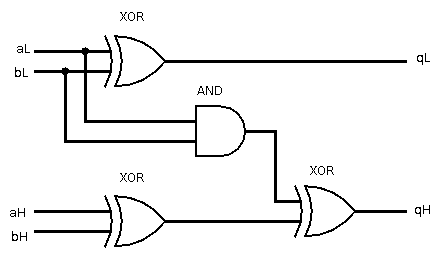
\includegraphics[scale=0.75]{SAT/adder_logisim.png}
\caption{Схема двухбитного сумматора}
\end{figure}

Сумматор здесь в самом простом возможном виде: у него нет входных и выходных переносов, и тут только 3 XOR-гейта
и один AND-гейт.
Попробуем разобраться, какой набор входных переменных заставит сумматор выставить оба выходных бита?
Просто подсчитав в уме, мы можем увидеть, что таких способа 4: $0+3=3$, $1+2=3$, $2+1=3$, $3+0=3$.
Вот также таблица истинности, с подсвеченными соответствующими рядами:

\newcommand{\HLcell}{\cellcolor{blue!25}}

\begin{center}
\begin{doublespace}
\noindent\(\begin{array}{l|llllll}
  & \text{aH} & \text{aL} & \text{bH} & \text{bL} & \text{qH} & \text{qL} \\
\hline
 \text{3+3 = 6 $\equiv $ 2 (mod 4)} & 1 & 1 & 1 & 1 & 1 & 0 \\
 \text{3+2 = 5 $\equiv $ 1 (mod 4)} & 1 & 1 & 1 & 0 & 0 & 1 \\
 \text{3+1 = 4 $\equiv $ 0 (mod 4)} & 1 & 1 & 0 & 1 & 0 & 0 \\
 \text{\HLcell{}3+0 = 3 $\equiv $ 3 (mod 4)} & \HLcell{}1 & \HLcell{}1 & \HLcell{}0 & \HLcell{}0 & \HLcell{}1 & \HLcell{}1 \\
 \text{2+3 = 5 $\equiv $ 1 (mod 4)} & 1 & 0 & 1 & 1 & 0 & 1 \\
 \text{2+2 = 4 $\equiv $ 0 (mod 4)} & 1 & 0 & 1 & 0 & 0 & 0 \\
 \text{\HLcell{}2+1 = 3 $\equiv $ 3 (mod 4)} & \HLcell{}1 & \HLcell{}0 & \HLcell{}0 & \HLcell{}1 & \HLcell{}1 & \HLcell{}1 \\
 \text{2+0 = 2 $\equiv $ 2 (mod 4)} & 1 & 0 & 0 & 0 & 1 & 0 \\
 \text{1+3 = 4 $\equiv $ 0 (mod 4)} & 0 & 1 & 1 & 1 & 0 & 0 \\
 \text{\HLcell{}1+2 = 3 $\equiv $ 3 (mod 4)} & \HLcell{}0 & \HLcell{}1 & \HLcell{}1 & \HLcell{}0 & \HLcell{}1 & \HLcell{}1 \\
 \text{1+1 = 2 $\equiv $ 2 (mod 4)} & 0 & 1 & 0 & 1 & 1 & 0 \\
 \text{1+0 = 1 $\equiv $ 1 (mod 4)} & 0 & 1 & 0 & 0 & 0 & 1 \\
 \text{\HLcell{}0+3 = 3 $\equiv $ 3 (mod 4)} & \HLcell{}0 & \HLcell{}0 & \HLcell{}1 & \HLcell{}1 & \HLcell{}1 & \HLcell{}1 \\
 \text{0+2 = 2 $\equiv $ 2 (mod 4)} & 0 & 0 & 1 & 0 & 1 & 0 \\
 \text{0+1 = 1 $\equiv $ 1 (mod 4)} & 0 & 0 & 0 & 1 & 0 & 1 \\
 \text{0+0 = 0 $\equiv $ 0 (mod 4)} & 0 & 0 & 0 & 0 & 0 & 0 \\
\end{array}\)
\end{doublespace}
\end{center}


Посмотрим, что об этом скажет SAT-солвер?

В начале, нам нужно представить наш двухбитный сумматор как CNF-выражение.

Используя Wolfram Mathematica, можно выразить 1-битное выражение для обоих выходов сумматоров:\\
\\
\textbf{\texttt{In[]:=AdderQ0[aL$\_$,bL$\_$]=Xor[aL,bL]}} \\
\textbf{\texttt{Out[]:=aL $\veebar$ bL}} \\
\\
\textbf{\texttt{In[]:=AdderQ1[aL$\_$,aH$\_$,bL$\_$,bH$\_$]=Xor[And[aL,bL],Xor[aH,bH]]}} \\
\textbf{\texttt{Out[]:=aH $\veebar$ bH $\veebar$ (aL \&\& bL)}} \\
\\
Нам нужно такое выражение, где обе части выдадут единицы.
Используя Wolfram Mathematica, найдем все возможные входы такого выражения (я склеил обе части при помощи And): \\
\\
\textbf{\texttt{In[]:=Boole[SatisfiabilityInstances[And[AdderQ0[aL,bL],AdderQ1[aL,aH,bL,bH]],\{aL,aH,bL,bH\},4]]}} \\
\textbf{\texttt{Out[]:=\{1,1,0,0\},\{1,0,0,1\},\{0,1,1,0\},\{0,0,1,1\}}} \\
\\
Да, действительно, Mathematica говорит, что здесь 4 входа, которые приведут к нужному нам результату.
Так что, Mathematica тоже может использоваться как \ac{SAT}-солвер.

Тем не менее, перейдем к CNF-форме. Используя Mathematica, сконвертируем наше выражение в CNF-форму:\\
\\
\textbf{\texttt{In[]:=cnf=BooleanConvert[And[AdderQ0[aL,bL],AdderQ1[aL,aH,bL,bH]],``CNF'']}} \\
\textbf{\texttt{Out[]:=(!aH $\|$ !bH) \&\& (aH $\|$ bH) \&\& (!aL $\|$ !bL) \&\& (aL $\|$ bL)}} \\
\\
Выглядит посложнее. Причина такой многословности в том, что \ac{CNF}-форма не поддерживает операцию исключающего
ИЛИ.
% FIXME: TeX form of the expression!

\subsubsection{MiniSat}

Для начала, попробуем MiniSat\footnote{\url{http://minisat.se/MiniSat.html}}.
Стандартный способ закодировать \ac{CNF}-выражение для MiniSat это перечислить все части ИЛИ в каждой строке.
Также, MiniSat не поддерживает имена переменных, только числа.
Перечислим наши переменные: 1 будет aH, 2 -- aL, 3 -- bH, 4 -- bL.

Вот что получилось, когда я сконвертировал выражение из Mathematica во входной файл для MiniSat:

\lstinputlisting{SAT/adder.cnf}

Две четверки в первой строке это, соответственно, число переменных и число клозов.
Так что тут 4 строки, каждая для каждого клоза ИЛИ.
Минус перед номером переменной означает что переменная инвертирована.
Отсутствие минуса -- не инвертирована.
Ноль в конце это просто оконечивающий ноль, означающий конец клоза.

Другими словами, каждая строка это ИЛИ-клоз с возможными инвертированиями,
и задача MiniSat в том, чтобы найти такой набор входных переменных, который удовлетворит все строки во входном файле.

Этот файл я назвал \textit{adder.cnf} и теперь попробуем MiniSat:

\begin{lstlisting}
% minisat -verb=0 adder.cnf results.txt
SATISFIABLE
\end{lstlisting}

Результаты в файле \textit{results.txt}:

\begin{lstlisting}
SAT
-1 -2 3 4 0
\end{lstlisting}

Это означает, что если первые две переменных (aH и aL) будут \textit{false},
и две последние переменные (bH и bL) будут \textit{true},
все \ac{CNF}-выражение будет истинно (satisfiable).
Похоже на правду: если bH и bL выставить в \textit{true}, оба бита результата также будут \textit{true}.

Как получить другие решения (instances)?
\ac{SAT}-солверы, как и \ac{SMT}-солверы, выдают только одно решение (или \textit{instance}).

MiniSat использует \ac{PRNG}, и его изначальное состояние (seed) можно задать явно.
Я попробовал разные значения, но результат всё тот же.
Тем не менее, CryptoMiniSat в этом случае может показать все возможные 4 решения, хотя и в хаотичном порядке.
Так что это не очень надежный способ.

Видимо, единственный способ, это инвертировать клоз решения и добавить его во входное выражение.
Мы получили \TT{-1 -2 3 4}, 
теперь мы можем инвертировать все значения в нем (просто поменяйте минусы: \TT{1 2 -3 -4}),
и добавим это в конец входного файла:

\begin{lstlisting}
p cnf 4 5
-1 -3 0
1 3 0
-2 -4 0
2 4 0
1 2 -3 -4
\end{lstlisting}

Получаем другой результат:

\begin{lstlisting}
SAT
1 2 -3 -4 0
\end{lstlisting}

Это означает что обе aH и aL должны быть \textit{true} и bH и bL должны быть \textit{false}, чтобы удовлетворить
входное выражение.
Снова инвертируем это решение и снова добавим:

\begin{lstlisting}
p cnf 4 6
-1 -3 0
1 3 0
-2 -4 0
2 4 0
1 2 -3 -4
-1 -2 3 4 0
\end{lstlisting}

Результат:

\begin{lstlisting}
SAT
-1 2 3 -4 0
\end{lstlisting}

aH=false, aL=true, bH=true, bL=false. Это также корректно, в соответствии с таблицей истинности.

Добавим снова:

\begin{lstlisting}
p cnf 4 7
-1 -3 0
1 3 0
-2 -4 0
2 4 0
1 2 -3 -4
-1 -2 3 4 0
1 -2 -3 4 0
\end{lstlisting}

\begin{lstlisting}
SAT
1 -2 -3 4 0
\end{lstlisting}

\textit{aH=true, aL=false, bH=false, bL=true.} Это тоже верно.

Это четвертый результат. Больше быть не должно. Что если добавим и это?

\begin{lstlisting}
p cnf 4 8
-1 -3 0
1 3 0
-2 -4 0
2 4 0
1 2 -3 -4
-1 -2 3 4 0
1 -2 -3 4 0
-1 2 3 -4 0
\end{lstlisting}

Теперь MiniSat просто говорит ``UNSATISFIABLE'' без всякой дополнительной информации в файле результатов.

Нам пример крохотный, но MiniSat может работать с огромными \ac{CNF}-выражениями.

\subsubsection{CryptoMiniSat}

Операция исключающего ИЛИ (XOR) отсутствует в CNF-форме, но она очень важна в криптографических алгоритмах.
Простейший способ представить одну единственную XOR-операцию в CNF-форме, это:
$(\neg x \vee \neg y) \wedge (x \vee y)$ -- не очень короткое выражение,
хотя, множество XOR-операций в одном выражении могут оптимизироваться лучше.

Одна значительная разница между MiniSat и CryptoMiniSat в том, что последний поддерживает
клозы с операцией XOR вместо ИЛИ,
потому что CryptoMiniSat предназначен больше для анализа криптоалгоритмов\footnote{\url{http://www.msoos.org/xor-clauses/}}.
XOR-клозы поддерживаются в CryptoMiniSat специальным образом, без трансляции в клозы ИЛИ.

Вам нужно просто прибавить ``x'' к клозу в \ac{CNF}-файле и CryptoMiniSat затем считает обычный ИЛИ-клоз как XOR-клоз.
Что до двухбитного сумматора, вот самое короткое из возможных XOR-CNF выражений, которое можно использовать
для поиска всех входных значений, где оба выходных бита выставлены:

$(aH \oplus bH) \wedge (aL \oplus bL)$

Это \TT{.cnf}-файл CryptoMiniSat:

\begin{lstlisting}
p cnf 4 2
x1 3 0
x2 4 0
\end{lstlisting}

Запускаю CryptoMiniSat с разными значениями для инициализации его \ac{PRNG} \dots

\begin{lstlisting}
% cryptominisat4 --verb 0 --random 0 XOR_adder.cnf
s SATISFIABLE
v 1 2 -3 -4 0
% cryptominisat4 --verb 0 --random 1 XOR_adder.cnf
s SATISFIABLE
v -1 -2 3 4 0
% cryptominisat4 --verb 0 --random 2 XOR_adder.cnf
s SATISFIABLE
v 1 -2 -3 4 0
% cryptominisat4 --verb 0 --random 3 XOR_adder.cnf
s SATISFIABLE
v 1 2 -3 -4 0
% cryptominisat4 --verb 0 --random 4 XOR_adder.cnf
s SATISFIABLE
v -1 2 3 -4 0
% cryptominisat4 --verb 0 --random 5 XOR_adder.cnf
s SATISFIABLE
v -1 2 3 -4 0
% cryptominisat4 --verb 0 --random 6 XOR_adder.cnf
s SATISFIABLE
v -1 -2 3 4 0
% cryptominisat4 --verb 0 --random 7 XOR_adder.cnf
s SATISFIABLE
v 1 -2 -3 4 0
% cryptominisat4 --verb 0 --random 8 XOR_adder.cnf
s SATISFIABLE
v 1 2 -3 -4 0
% cryptominisat4 --verb 0 --random 9 XOR_adder.cnf
s SATISFIABLE
v 1 2 -3 -4 0
\end{lstlisting}

Тем не менее, все 4 возможных решения, это:

\begin{lstlisting}
v -1 -2 3 4 0
v -1 2 3 -4 0
v 1 -2 -3 4 0
v 1 2 -3 -4 0
\end{lstlisting}

\dots то же, что и выдал MiniSat.

\subsection{Picosat}

По крайней мере Picosat может перечислить все возможные решения без тех костылей, которые я только что показывал:

\begin{lstlisting}
% picosat --all adder.cnf
s SATISFIABLE
v -1 -2 3 4 0
s SATISFIABLE
v -1 2 3 -4 0
s SATISFIABLE
v 1 2 -3 -4 0
s SATISFIABLE
v 1 -2 -3 4 0
s SOLUTIONS 4
\end{lstlisting}

% subsections:
\subsection{Задача о восьми ферзях}
\label{EightQueens}

Восемь ферзей это популярная задача, и она часто используется для измерения скорости работы SAT-солверов.
Нужно расставить на шахматной доске 8 ферзей так, чтобы они не атаковали друг друга.
Например:

\begin{lstlisting}
| | | |*| | | | |
| | | | | | |*| |
| | | | |*| | | |
| |*| | | | | | |
| | | | | |*| | |
|*| | | | | | | |
| | |*| | | | | |
| | | | | | | |*|
\end{lstlisting}

Попробуем разобраться, как её решить.

\subsubsection{make\_one\_hot}
\label{POPCNTOne}

Одна важная ф-ция, которую мы будем (часто) использовать это \TT{make\_one\_hot}.
Это ф-ция, которая возвращает \textit{Истинно}, если один из входов истинен, остальные ложны.
Она вернет \textit{Ложно} в остальных случаях.

В моих других примерах, я использовал Wolfram Mathematica для генерирования CNF-клозов для этого, например: \ref{minesweeper_SAT}.
Какое выражение сгенерирует Mathematica для ф-ции \TT{make\_one\_hot} для 8-и входов?

\begin{lstlisting}
(!a||!b)&&(!a||!c)&&(!a||!d)&&(!a||!e)&&(!a||!f)&&(!a||!g)&&(!a||!h)&&(a||b||c||d||e||f||g||h)&&
(!b||!c)&&(!b||!d)&&(!b||!e)&&(!b||!f)&&(!b||!g)&&(!b||!h)&&(!c||!d)&&(!c||!e)&&(!c||!f)&&(!c||!g)&&
(!c||!h)&&(!d||!e)&&(!d||!f)&&(!d||!g)&&(!d||!h)&&(!e||!f)&&(!e||!g)&&(!e||!h)&&(!f||!g)&&(!f||!h)&&(!g||!h)
\end{lstlisting}

Мы можем ясно увидеть что выражение состоит из всех возможных пар переменных (инвертированных) плюс
перечисление всех переменных (не инвертированных).
На обычном русском языке это означает: ``ни одна пара не должна быть равна двум \textit{Истинно} \textit{И}
по крайней мере одно \textit{Истинно} должно
присутствовать среди переменных''.

Вот как это работает: если две переменных будут \textit{Истино}, инвертированными они обе будут \textit{Ложно},
и этот клоз не будет
вычислен как \textit{Истинно}, а это наша конечная цель.
Если одна из переменных будет \textit{Истинно}, инвертированными, одна будет \textit{Истинно},
вторая \textit{Ложно} (хорошо).
Если обе переменных будут \textit{Ложно}, инвертированными, они обе будут \textit{Истинно} (тоже хорошо).

Вот как мы можем сгенерировать клозы для этой ф-ции используя модуль \textit{itertools} из Питона,
который также содержит много важных ф-ций из комбинаторики:

\begin{lstlisting}
    # naive/pairwise encoding   
    def AtMost1(self, lst):
        for pair in itertools.combinations(lst, r=2):
            self.add_clause([self.neg(pair[0]), self.neg(pair[1])])
       
    # make one-hot (AKA unitary) variable
    def make_one_hot(self, lst):
        self.AtMost1(lst)
        self.OR_always(lst)
\end{lstlisting}

Ф-ция \TT{AtMost1()} перечисляет все возможные пары используя ф-цию \textit{combinations()} из
\textit{itertools}.

Ф-ция \TT{make\_one\_hot()} делает то же самое, только добавляет последний клоз, который заставляет иметь хотя бы одну
переменную, равную Истинно.

Какие клозы будут сгенерированы для 5-и переменных (1..5)?

\lstinputlisting{SAT/8queens/popcnt1.cnf}

Да, это все возможные пары чисел 1..5 + все 5 чисел.

Можем посмотреть все решения используя Picosat:

\begin{lstlisting}
% picosat --all popcnt1.cnf

s SATISFIABLE
v -1 -2 -3 -4 5 0
s SATISFIABLE
v -1 -2 -3 4 -5 0
s SATISFIABLE
v -1 -2 3 -4 -5 0
s SATISFIABLE
v -1 2 -3 -4 -5 0
s SATISFIABLE
v 1 -2 -3 -4 -5 0
s SOLUTIONS 5
\end{lstlisting}

Действительно, 5 возможных решений.

\subsubsection{Восемь ферзей}

Теперь вернемся назад к восьми ферзям.

Мы можем назначить 64 переменных для $8 \cdot 8=64$ клеток.
Клетка на которой есть ферзь будет равна \textit{Истинно}, пустая клетка будет \textit{Ложно}.

Проблема расположения неатакующих (друг друга) ферзей на шахматной доске (любого размера), на обычном русском
языке может быть выражена так:

\begin{itemize}
\item один единственный ферзь должен присутствовать в каждом ряду;

\item один единственный ферзь должен присутствовать в каждом столбце;

\item или один ферзь должен присутствовать на каждой диагонали, или вовсе отсутствовать (пустые диагонали могут быть
и в правильном решении).
\end{itemize}

Эти правила можно перевести так:

\begin{itemize}
\item make\_one\_hot(каждый ряд)==\textit{Истинно}

\item make\_one\_hot(каждый столбец)==\textit{Истинно}

\item AtMost1(каждая диагональ)==\textit{Истинно}
\end{itemize}

Теперь мы должны перечислить ряды, столбцы и диагонали, и собрать все клозы:

\lstinputlisting{SAT/8queens/8queens.py}
( \url{https://github.com/DennisYurichev/SAT_SMT_article/blob/master/SAT/8queens/8queens.py} )

Возможно, ф-ция \TT{gen\_diagonal()} выглядит не очень эстетично:
она перечисляет также поддиагонали более длинных диагоналей, которые уже были раннее.
Чтобы не было повторяющихся клозов, глобальная переменная \textit{clauses} это не список, а множество,
которое может содержать в себе только уникальные данные.

Также, я использовал ф-цию \TT{AtMost1} для каждого столбца, это поможет генерировать чуть меньше клозов.
Каждый столбец будет содержать ферзя в любом случае, это следует из первого правила (\TT{make\_one\_hot} для каждого ряда).

После запуска, получаем CNF-файл с 64-я переменными и 736-я клозами (\url{https://github.com/DennisYurichev/SAT_SMT_article/blob/master/SAT/8queens/8queens.cnf}).
Вот одно из решений:

\begin{lstlisting}
% python 8queens.py
len(clauses)= 736
| | | |*| | | | |
| | | | | | |*| |
| | | | |*| | | |
| |*| | | | | | |
| | | | | |*| | |
|*| | | | | | | |
| | |*| | | | | |
| | | | | | | |*|
\end{lstlisting}

Как много здесь возможных решений?
Picosat говорит что 92, что действительно корректное число решений (\url{https://oeis.org/A000170}).

Скорость Picosat не очень впечатляет, вероятно потому что ему приходится выводить все решения.
Моему древнему нетбуку с Intel Atom 1.66GHz, понадобилось 34 для перечисления всех решений для шахматной доски
$11 \cdot 11$ 
(2680 решения),
что намного медленнее, чем моя прямолинейная программа полного перебора: \url{https://yurichev.com/blog/8queens/}.
Тем не менее, для поиска первого решения, Picosat работает крайне быстро (как и другие SAT-солверы).

Эта SAT-задача также достаточно проста, чтобы её можно было легко решить при помощи моего простейшего
SAT-солвера, работающего на базе поиска с возвратом (\textit{backtracking}):
\ref{SAT_backtrack}.

\subsubsection{Подсчет всех решений}

Мы получаем решение, инвертируем его и добавляем как новый констрайнт.
На обычном русском языке это звучит ``найди решение, котороые также не ровно тому, что мы только что нашли/добавили''.
Мы добавляем их последовательно, и процесс замедляется --- потому что размер проблемы (\textit{instance}) растет 
и SAT-солверу всё труднее находить новое решение.

\subsubsection{Пропуск симметрических решений}

Мы также можем добавлять повернутое и отраженное (горизонтально) решение, чтобы пропускать симметрические решения.
Делая так, мы получаем 12 решений для доски 8*8, 46 для 9*9, итд.
Это \url{https://oeis.org/A002562}.


\subsection{Sudoku в SAT}
\label{Sudoku_SAT}

Кто-то может подумать, что мы можем закодировать каждое число 1..9 в двоичном виде: 5 бит или переменных было бы достаточно.
Но есть даже еще более простой способ: выделить 9 бит, где только один бит будет \textit{Истинен}.
Число 1 может быт закодировано как [1, 0, 0, 0, 0, 0, 0, 0, 0], число 3 как [0, 0, 1, 0, 0, 0, 0, 0, 0], итд.
Выглядит неэкономично? Да, но другие операции будут проще.

Прежде всего, мы будем снова использовать важную ф-цию \TT{POPCNT1}, которую я описывал раннее: \ref{POPCNTOne}.

Вторая нужная нам важная операция, которую нам нужно придумать, это как сделать 9 чисел уникальными.
Если каждое число закодировано как 9-битный вектор, 9 чисел могут сформировать матрицу, вроде:

\begin{lstlisting}
0 0 0 0 0 0 1 0 0 <- §1-е§ число
0 0 0 0 0 1 0 0 0 <- §2-е§ число
0 1 0 0 0 0 0 0 0 <- ...
0 0 1 0 0 0 0 0 0 <- ...
0 0 0 0 0 0 0 0 1 <- ...
0 0 0 0 1 0 0 0 0 <- ...
0 0 0 0 0 0 0 1 0 <- ...
1 0 0 0 0 0 0 0 0 <- ...
0 0 0 1 0 0 0 0 0 <- §9-е§ число
\end{lstlisting}

Теперь будем использовать ф-цию \TT{POPCNT1} чтобы сделать каждый ряд в матрице содержащим только один бит \textit{Истина},
и это будет сохранять корректность нашего способа кодирования, т.к., вектор не может иметь более одного бита \textit{Истина},
либо не иметь битов \textit{Истина} вообще.
Затем мы будем использовать ф-цию \TT{POPCNT1} снова чтобы сделать так, чтобы каждый столбец в матрице имел только
один единственный бит \textit{Истина}.
Это сделает все ряды в матрице уникальными, другими словами, все 9 закодированных чисел всегда будут уникальными.

После применения ф-ции \TT{POPCNT1} 9+9=18 раз, у нас будет 9 уникальных чисел в пределах 1..9.

Используя эту операцию мы можем сделать каждый ряд в головоломке Судоку уникальным, каждый столбец уникальным,
и каждый квадрат $3 \cdot 3=9$ тоже уникальным.

\lstinputlisting{SAT/sudoku/sudoku_SAT.py}
( \url{https://github.com/DennisYurichev/SAT_SMT_article/blob/master/SAT/sudoku/sudoku_SAT.py} )

Ф-ция \TT{make\_distinct\_bits\_in\_vector()} сохраняет корректность кодирования.\\
Ф-ция \TT{make\_distinct\_vectors()} делает 9 чисел уникальными.\\
Ф-ция \TT{cvt\_vector\_to\_number()} декодирует вектор в число.\\
Ф-ция \TT{number\_to\_vector()} кодирует число в вектор.\\
Ф-ция \TT{main()} содержит все необходимые вызовы, чтобы сделать уникальными ряды/столбцы и квадраты $3\cdot 3$.

Работает:

\begin{lstlisting}
% python sudoku_SAT.py
len(clauses)= 12195
1 4 5 3 2 7 6 9 8
8 3 9 6 5 4 1 2 7
6 7 2 9 1 8 5 4 3
4 9 6 1 8 5 3 7 2
2 1 8 4 7 3 9 5 6
7 5 3 2 9 6 4 8 1
3 6 7 5 4 2 8 1 9
9 8 4 7 6 1 2 3 5
5 2 1 8 3 9 7 6 4
\end{lstlisting}

Такое же решение как и раннее: \ref{sudoku_SMT}.

Picosat говорит что эта SAT-проблема имеет только одно решение.
Действительно, как говорят, настоящая головоломка Судоку может иметь только одно решение.

\subsubsection{Избавление от одного вызова POPCNT1}
\label{OR_in_POPCNT1}

Чтобы сделать 9 уникальный чисел 1..9 мы можем использовать ф-цию \TT{POPCNT1}, чтобы сделать уникальным каждый ряд
в матрице, и использовать операцию \textit{ИЛИ} для всех столбцов.
Это будет иметь такой же эффект: все ряды должны быть уникальны, чтобы каждый столбец вычислялся в \textit{Истино}
после применения операции \textit{ИЛИ} ко всем переменным в столбце.
(Я буду делать так в следующем примере: \ref{Zebra_SAT}.)

Это приведет к тому, что будет 3447 клозов вместо 12195, но почему-то, SAT-солверы работают медленнее. Не знаю, почему.


% TODO translate src
\subsection{Головоломка Зебры как SAT-проблема}
\label{Zebra_SAT}

Попробуем решить головоломку Зебры (\ref{zebra_SMT}) в SAT.

Я определю каждую переменную как вектор из пяти переменных, как я делал это раннее в солвере Судоку: \ref{Sudoku_SAT}.

Я также использую ф-цию \TT{POPCNT1}, но в отличие от предыдущего примера,
я использовал Wolfram Mathematica для генерирования её в CNF-форме:

\begin{lstlisting}
In[]:= tbl1=Table[PadLeft[IntegerDigits[i,2],5] ->If[Equal[DigitCount[i,2][[1]],1],1,0],{i,0,63}]
Out[]= {{0,0,0,0,0}->0,
{0,0,0,0,1}->1,
{0,0,0,1,0}->1,
{0,0,0,1,1}->0,
{0,0,1,0,0}->1,
{0,0,1,0,1}->0,

...

{1,1,1,1,0}->0,
{1,1,1,1,1}->0}

In[]:= BooleanConvert[BooleanFunction[tbl1,{a,b,c,d,e}],"CNF"]
Out[]= (!a||!b)&&(!a||!c)&&(!a||!d)&&(!a||!e)&&(a||b||c||d||e)&&(!b||!c)&&(!b||!d)&&(!b||!e)&&(!c||!d)&&(!c||!e)&&(!d||!e)
\end{lstlisting}

Также, как я предлагал раньше (\ref{OR_in_POPCNT1}), я использовал операцию \textit{ИЛИ} для второго шага.

\begin{lstlisting}
def mathematica_to_CNF (s, d):
    for k in d.keys():
        s=s.replace(k, d[k])
    s=s.replace("!", "-").replace("||", " ").replace("(", "").replace(")", "")
    s=s.split ("&&")
    return s

def add_popcnt1(v1, v2, v3, v4, v5):
    global clauses
    s="(!a||!b)&&" \
      "(!a||!c)&&" \
      "(!a||!d)&&" \
      "(!a||!e)&&" \
      "(!b||!c)&&" \
      "(!b||!d)&&" \
      "(!b||!e)&&" \
      "(!c||!d)&&" \
      "(!c||!e)&&" \
      "(!d||!e)&&" \
      "(a||b||c||d||e)"

    clauses=clauses+mathematica_to_CNF(s, {"a":v1, "b":v2, "c":v3, "d":v4, "e":v5})

...

# k=tuple: ("high-level" variable name, number of bit (0..4))
# v=variable number in CNF
vars={}
vars_last=1

...

def alloc_distinct_variables(names):
    global vars
    global vars_last
    for name in names:
        for i in range(5):
            vars[(name,i)]=str(vars_last)
            vars_last=vars_last+1

        add_popcnt1(vars[(name,0)], vars[(name,1)], vars[(name,2)], vars[(name,3)], vars[(name,4)])

    # make them distinct:
    for i in range(5):
        clauses.append(vars[(names[0],i)] + " " + vars[(names[1],i)] + " " + vars[(names[2],i)] + " " + vars[(names[3],i)] + " " + vars[(names[4],i)])

...

alloc_distinct_variables(["Yellow", "Blue", "Red", "Ivory", "Green"])
alloc_distinct_variables(["Norwegian", "Ukrainian", "Englishman", "Spaniard", "Japanese"])
alloc_distinct_variables(["Water", "Tea", "Milk", "OrangeJuice", "Coffee"])
alloc_distinct_variables(["Kools", "Chesterfield", "OldGold", "LuckyStrike", "Parliament"])
alloc_distinct_variables(["Fox", "Horse", "Snails", "Dog", "Zebra"])

...

\end{lstlisting}

Теперь у нас пять булевых переменных для каждой \textit{высокоуровневной} переменной,
и каждая группа переменных гарантированно будет иметь разные значения.

Теперь перечитаем условие головоломки: ``2. Англичанин живёт в красном доме.''.
Это легко.
В моих примерах на Z3 и KLEE я просто написал ``Englishman==Red''.
Та же история и здесь: мы просто добавляем клозы, показывающие, что 5 булевых переменных для ``Englishman''
должны равняться пяти переменных для ``Red''.

На самом низком уровне CNF, если мы хотим сказать, что две переменных должны равняться друг другу,
мы добавляем два клоза:

$(var1 \vee \neg var2) \wedge (\neg var1 \vee var2)$

Это означает что значения обоих \textit{var1} и \textit{var2} должны быть или \textit{Ложно} или \textit{Истинно},
но они не могут быть разными.

\begin{lstlisting}
def add_eq_clauses(var1, var2):
    global clauses
    clauses.append(var1 + " -" + var2)
    clauses.append("-"+var1 + " " + var2)

def add_eq (n1, n2):
    for i in range(5):
        add_eq_clauses(vars[(n1,i)], vars[(n2, i)])

...

# 2.The Englishman lives in the red house.
add_eq("Englishman","Red")

# 3.The Spaniard owns the dog.
add_eq("Spaniard","Dog")

# 4.Coffee is drunk in the green house.
add_eq("Coffee","Green")

...

\end{lstlisting}

Теперь следующие условия:
``9. В центральном доме пьют молоко.'' (т.е., в третьем доме), ``10. Норвежец живёт в первом доме.''
Мы можем присвоить булевы значения напрямую:

\begin{lstlisting}
# n=1..5
def add_eq_var_n (name, n):
    global clauses
    global vars
    for i in range(5):
        if i==n-1:
            clauses.append(vars[(name,i)]) # always True
        else:
            clauses.append("-"+vars[(name,i)]) # always False

...

# 9.Milk is drunk in the middle house.
add_eq_var_n("Milk",3) # i.e., 3rd house

# 10.The Norwegian lives in the first house.
add_eq_var_n("Norwegian",1)
\end{lstlisting}

Для ``Milk'' у нас значение ``0 0 1 0 0'', для ``Norwegian'': ``1 0 0 0 0''.

Что делать с этим?
``6. Зелёный дом стоит сразу справа от белого дома.''
Я могу сконструировать такое условие:

\begin{lstlisting}
    Ivory      Green
AND(1 0 0 0 0  0 1 0 0 0)
.. OR ..
AND(0 1 0 0 0  0 0 1 0 0)
.. OR ..
AND(0 0 1 0 0  0 0 0 1 0)
.. OR ..
AND(0 0 0 1 0  0 0 0 0 1)
\end{lstlisting}

Для ``белого/ivory'' тут нет ``0 0 0 0 1'', потому что он не может быть последним.
Теперь я конвертирую эти условия в CNF при помощи Wolfram Mathematica:

\begin{lstlisting}
In[]:= BooleanConvert[(a1&& !b1&&!c1&&!d1&&!e1&&!a2&& b2&&!c2&&!d2&&!e2) ||
(!a1&& b1&&!c1&&!d1&&!e1&&!a2&& !b2&&c2&&!d2&&!e2) ||
(!a1&& !b1&&c1&&!d1&&!e1&&!a2&& !b2&&!c2&&d2&&!e2) ||
(!a1&& !b1&&!c1&&d1&&!e1&&!a2&& !b2&&!c2&&!d2&&e2) ,"CNF"]

Out[]= (!a1||!b1)&&(!a1||!c1)&&(!a1||!d1)&&(a1||b1||c1||d1)&&!a2&&(!b1||!b2)&&(!b1||!c1)&&
(!b1||!d1)&&(b1||b2||c1||d1)&&(!b2||!c1)&&(!b2||!c2)&&(!b2||!d1)&&(!b2||!d2)&&(!b2||!e2)&&
(b2||c1||c2||d1)&&(b2||c2||d1||d2)&&(b2||c2||d2||e2)&&(!c1||!c2)&&(!c1||!d1)&&(!c2||!d1)&&
(!c2||!d2)&&(!c2||!e2)&&(!d1||!d2)&&(!d2||!e2)&&!e1
\end{lstlisting}

И вот фрагмент моего кода на Питоне:

\begin{lstlisting}
def add_right (n1, n2):
    global clauses
    s="(!a1||!b1)&&(!a1||!c1)&&(!a1||!d1)&&(a1||b1||c1||d1)&&!a2&&(!b1||!b2)&&(!b1||!c1)&&(!b1||!d1)&&" \
      "(b1||b2||c1||d1)&&(!b2||!c1)&&(!b2||!c2)&&(!b2||!d1)&&(!b2||!d2)&&(!b2||!e2)&&(b2||c1||c2||d1)&&" \
      "(b2||c2||d1||d2)&&(b2||c2||d2||e2)&&(!c1||!c2)&&(!c1||!d1)&&(!c2||!d1)&&(!c2||!d2)&&(!c2||!e2)&&" \
      "(!d1||!d2)&&(!d2||!e2)&&!e1"

    clauses=clauses+mathematica_to_CNF(s, {
	"a1": vars[(n1,0)], "b1": vars[(n1,1)], "c1": vars[(n1,2)], "d1": vars[(n1,3)], "e1": vars[(n1,4)],
	"a2": vars[(n2,0)], "b2": vars[(n2,1)], "c2": vars[(n2,2)], "d2": vars[(n2,3)], "e2": vars[(n2,4)]})

...

# 6.The green house is immediately to the right of the ivory house.
add_right("Ivory", "Green")
\end{lstlisting}

Что мы будем делать с этим?
``11. Сосед того, кто курит Chesterfield, держит лису.''
``12. В доме по соседству с тем, в котором держат лошадь, курят Kool.''

Мы не знаем с какой стороны, слева или справа, но знаем что они отличаются на единицу.
Вот какие клозы я добавлю:

\begin{lstlisting}
    Chesterfield  Fox
AND(0 0 0 0 1     0 0 0 1 0)
.. OR ..
AND(0 0 0 1 0     0 0 0 0 1)
AND(0 0 0 1 0     0 0 1 0 0)
.. OR ..
AND(0 0 1 0 0     0 1 0 0 0)
AND(0 0 1 0 0     0 0 0 1 0)
.. OR ..
AND(0 1 0 0 0     1 0 0 0 0)
AND(0 1 0 0 0     0 0 1 0 0)
.. OR ..
AND(1 0 0 0 0     0 1 0 0 0)
\end{lstlisting}

И снова могу сконвертировать это всё в CNF при помощи Mathematica:

\begin{lstlisting}
In[]:= BooleanConvert[(a1&& !b1&&!c1&&!d1&&!e1&&!a2&& b2&&!c2&&!d2&&!e2) ||

(!a1&& b1&&!c1&&!d1&&!e1&&a2&& !b2&&!c2&&!d2&&!e2) ||
(!a1&& b1&&!c1&&!d1&&!e1&&!a2&& !b2&&c2&&!d2&&!e2) ||

(!a1&& !b1&&c1&&!d1&&!e1&&!a2&& b2&&!c2&&!d2&&!e2) ||
(!a1&& !b1&&c1&&!d1&&!e1&&!a2&& !b2&&!c2&&d2&&!e2) ||

(!a1&& !b1&&!c1&&d1&&!e1&&!a2&& !b2&&c2&&!d2&&!e2) ||
(!a1&& !b1&&!c1&&d1&&!e1&&!a2&& !b2&&!c2&&!d2&&e2) ||

(!a1&& !b1&&!c1&&!d1&&e1&&!a2&& !b2&&!c2&&d2&&!e2) ,"CNF"]

Out[]= (!a1||!b1)&&(!a1||!c1)&&(!a1||!d1)&&(!a1||!e1)&&(a1||b1||c1||d1||e1)&&(!a2||b1)&&(!a2||!b2)&&
(!a2||!c2)&&(!a2||!d2)&&(!a2||!e2)&&(a2||b2||c1||c2||d1||e1)&&(a2||b2||c2||d1||d2)&&(a2||b2||c2||d2||e2)&&
(!b1||!b2)&&(!b1||!c1)&&(!b1||!d1)&&(!b1||!e1)&&(b1||b2||c1||d1||e1)&&(!b2||!c2)&&(!b2||!d1)&&(!b2||!d2)&&
(!b2||!e1)&&(!b2||!e2)&&(!c1||!c2)&&(!c1||!d1)&&(!c1||!e1)&&(!c2||!d2)&&(!c2||!e1)&&(!c2||!e2)&&
(!d1||!d2)&&(!d1||!e1)&&(!d2||!e2)
\end{lstlisting}

И вот мой код:

\begin{lstlisting}
def add_right_or_left (n1, n2):
    global clauses
    s="(!a1||!b1)&&(!a1||!c1)&&(!a1||!d1)&&(!a1||!e1)&&(a1||b1||c1||d1||e1)&&(!a2||b1)&&" \
      "(!a2||!b2)&&(!a2||!c2)&&(!a2||!d2)&&(!a2||!e2)&&(a2||b2||c1||c2||d1||e1)&&(a2||b2||c2||d1||d2)&&" \
       "(a2||b2||c2||d2||e2)&&(!b1||!b2)&&(!b1||!c1)&&(!b1||!d1)&&(!b1||!e1)&&(b1||b2||c1||d1||e1)&&" \
       "(!b2||!c2)&&(!b2||!d1)&&(!b2||!d2)&&(!b2||!e1)&&(!b2||!e2)&&(!c1||!c2)&&(!c1||!d1)&&(!c1||!e1)&&" \
       "(!c2||!d2)&&(!c2||!e1)&&(!c2||!e2)&&(!d1||!d2)&&(!d1||!e1)&&(!d2||!e2)"
    
    clauses=clauses+mathematica_to_CNF(s, {
	"a1": vars[(n1,0)], "b1": vars[(n1,1)], "c1": vars[(n1,2)], "d1": vars[(n1,3)], "e1": vars[(n1,4)],
	"a2": vars[(n2,0)], "b2": vars[(n2,1)], "c2": vars[(n2,2)], "d2": vars[(n2,3)], "e2": vars[(n2,4)]})

...

# 11.The man who smokes Chesterfields lives in the house next to the man with the fox.
add_right_or_left("Chesterfield","Fox") # left or right

# 12.Kools are smoked in the house next to the house where the horse is kept.
add_right_or_left("Kools","Horse") # left or right
\end{lstlisting}

Вот и всё!
Полный исходный код: \url{https://github.com/DennisYurichev/SAT_SMT_article/blob/master/SAT/zebra/zebra_SAT.py}.

Итоговая CNF-проблема имеет 125 булевых переменных и 511 клозов: \\
\url{https://github.com/DennisYurichev/SAT_SMT_article/blob/master/SAT/zebra/1.cnf}.
Это очень легкая задача для любого SAT-солвера.
Даже мой игрушечный SAT-солвер (\ref{SAT_backtrack}) может решить её за \textasciitilde{}1 секунду на моем древнем
нетбуке с Intel Atom.

И конечно же, тут только одно решение, что и подтверждается при помощи Picosat.

\begin{lstlisting}
% python zebra_SAT.py
Yellow 1
Blue 2
Red 3
Ivory 4
Green 5
Norwegian 1
Ukrainian 2
Englishman 3
Spaniard 4
Japanese 5
Water 1
Tea 2
Milk 3
OrangeJuice 4
Coffee 5
Kools 1
Chesterfield 2
OldGold 3
LuckyStrike 4
Parliament 5
Fox 1
Horse 2
Snails 3
Dog 4
Zebra 5
\end{lstlisting}


\subsection{Взлом Сапёра при помощи SAT}
\label{minesweeper_SAT}

См.также о взломе оного при помощи Z3: \ref{minesweeper_SMT}.

\subsubsection{Простая ф-ция подсчета бит (\textit{population count})}

Прежде всего, нам нужно как считать количество соседних бомб.
Ф-ция подсчета та же, что и ф-ция подсчета бит (\textit{population count}).

Мы можем создать \ac{CNF}-выражение используя Wolfram Mathematica.
Это будет ф-ция, возвращающая \textit{True} если любые из двух бит 8-битного входа равняются \textit{True},
а остальные --- \textit{False}.
В начале, сделаем таблицу истинности для такой ф-ции:

\begin{lstlisting}
In[]:= tbl2 = 
 Table[PadLeft[IntegerDigits[i, 2], 8] -> 
   If[Equal[DigitCount[i, 2][[1]], 2], 1, 0], {i, 0, 255}]

Out[]= {{0, 0, 0, 0, 0, 0, 0, 0} -> 0, {0, 0, 0, 0, 0, 0, 0, 1} -> 0, 
{0, 0, 0, 0, 0, 0, 1, 0} -> 0, {0, 0, 0, 0, 0, 0, 1, 1} -> 1, 
{0, 0, 0, 0, 0, 1, 0, 0} -> 0, {0, 0, 0, 0, 0, 1, 0, 1} -> 1, 
{0, 0, 0, 0, 0, 1, 1, 0} -> 1, {0, 0, 0, 0, 0, 1, 1, 1} -> 0, 
{0, 0, 0, 0, 1, 0, 0, 0} -> 0, {0, 0, 0, 0, 1, 0, 0, 1} -> 1, 
{0, 0, 0, 0, 1, 0, 1, 0} -> 1, {0, 0, 0, 0, 1, 0, 1, 1} -> 0, 
...
{1, 1, 1, 1, 1, 0, 1, 0} -> 0, {1, 1, 1, 1, 1, 0, 1, 1} -> 0, 
{1, 1, 1, 1, 1, 1, 0, 0} -> 0, {1, 1, 1, 1, 1, 1, 0, 1} -> 0, 
{1, 1, 1, 1, 1, 1, 1, 0} -> 0, {1, 1, 1, 1, 1, 1, 1, 1} -> 0}
\end{lstlisting}

Теперь можем сделать \ac{CNF}-выражение используя эту таблицу истинности:

\begin{lstlisting}
In[]:= BooleanConvert[
 BooleanFunction[tbl2, {a, b, c, d, e, f, g, h}], "CNF"]

Out[]= (! a || ! b || ! c) && (! a || ! b || ! d) && (! a || ! 
    b || ! e) && (! a || ! b || ! f) && (! a || ! b || ! g) && (! 
    a || ! b || ! h) && (! a || ! c || ! d) && (! a || ! c || ! 
    e) && (! a || ! c || ! f) && (! a || ! c || ! g) && (! a || ! 
    c || ! h) && (! a || ! d || ! e) && (! a || ! d || ! f) && (! 
    a || ! d || ! g) && (! a || ! d || ! h) && (! a || ! e || ! 
    f) && (! a || ! e || ! g) && (! a || ! e || ! h) && (! a || ! 
    f || ! g) && (! a || ! f || ! h) && (! a || ! g || ! h) && (a || 
   b || c || d || e || f || g) && (a || b || c || d || e || f || 
   h) && (a || b || c || d || e || g || h) && (a || b || c || d || f ||
    g || h) && (a || b || c || e || f || g || h) && (a || b || d || 
   e || f || g || h) && (a || c || d || e || f || g || 
   h) && (! b || ! c || ! d) && (! b || ! c || ! e) && (! b || ! 
    c || ! f) && (! b || ! c || ! g) && (! b || ! c || ! h) && (! 
    b || ! d || ! e) && (! b || ! d || ! f) && (! b || ! d || ! 
    g) && (! b || ! d || ! h) && (! b || ! e || ! f) && (! b || ! 
    e || ! g) && (! b || ! e || ! h) && (! b || ! f || ! g) && (! 
    b || ! f || ! h) && (! b || ! g || ! h) && (b || c || d || e || 
   f || g || 
   h) && (! c || ! d || ! e) && (! c || ! d || ! f) && (! c || ! 
    d || ! g) && (! c || ! d || ! h) && (! c || ! e || ! f) && (! 
    c || ! e || ! g) && (! c || ! e || ! h) && (! c || ! f || ! 
    g) && (! c || ! f || ! h) && (! c || ! g || ! h) && (! d || ! 
    e || ! f) && (! d || ! e || ! g) && (! d || ! e || ! h) && (! 
    d || ! f || ! g) && (! d || ! f || ! h) && (! d || ! g || ! 
    h) && (! e || ! f || ! g) && (! e || ! f || ! h) && (! e || ! 
    g || ! h) && (! f || ! g || ! h)
\end{lstlisting}

Синтаксис такой же как и в Си/Си++
Проверим.

Я написал Питоновскую ф-цию для конвертирования вывода Mathematica в \ac{CNF}-файл, который можно подать на вход
SAT-солверу:

\lstinputlisting{SAT/minesweeper/tst.py}

Она заменяет переменные a/b/c/... на переданные имена переменных (1/2/3...), перерабатыает синтаксис, итд.
Вот результат:

\lstinputlisting{SAT/minesweeper/tst1.cnf}

Могу запустить:

\begin{lstlisting}
% minisat -verb=0 tst1.cnf results.txt
SATISFIABLE

% cat results.txt
SAT
1 -2 -3 -4 -5 -6 -7 8 0
\end{lstlisting}

Имя переменной в результате без знака минуса, это \textit{True}.
Имя переменной со знаком минус, это \textit{False}.
Мы здесь видим только две переменных \textit{True}: 1 и 8.
Это действительно корректно: солвер MiniSat нашел условие, для которого наша ф-ция возвращает \textit{True}.
Ноль в конце это просто терминирующий символ, который ничего не означает.

Мы можем попросить MiniSat найти еще одно решение, добавив текущее решение во входной CNF-файл,
но где все переменные инвертированы:

\begin{lstlisting}
...
-5 -6 -8 0
-5 -7 -8 0
-6 -7 -8 0
-1 2 3 4 5 6 7 -8 0
\end{lstlisting}

В обычном русском языке, это означает ``дайте ЛЮБОЕ решение, которые удовлетворяет все клозы, но также не равно
последнему клозу, которое мы только что добавили''.

MiniSat, действительно, находит еще одно решение, и снова, только с двумя переменными, равными \textit{True}:

\begin{lstlisting}
% minisat -verb=0 tst2.cnf results.txt
SATISFIABLE

% cat results.txt
SAT
1 2 -3 -4 -5 -6 -7 -8 0
\end{lstlisting}

Кстати, ф-ция \textit{population count} для 8-и соседей (POPCNT8) в CNF-форме, самая простая:

\begin{lstlisting}
a&&b&&c&&d&&e&&f&&g&&h
\end{lstlisting}

Действительно: она истинна, если все 8 входных бит тоже истинны.

Ф-ция для отсутствия соседей (POPCNT0) тоже очень простая:

\begin{lstlisting}
!a&&!b&&!c&&!d&&!e&&!f&&!g&&!h
\end{lstlisting}

Это означает, что она вернет \textit{True}, если все входные переменные \textit{False}.

Кстати, ф-ция POPCNT1 тоже простая:

\begin{lstlisting}
(!a||!b)&&(!a||!c)&&(!a||!d)&&(!a||!e)&&(!a||!f)&&(!a||!g)&&(!a||!h)&&(a||b||c||d||e||f||g||h)&&
(!b||!c)&&(!b||!d)&&(!b||!e)&&(!b||!f)&&(!b||!g)&&(!b||!h)&&(!c||!d)&&(!c||!e)&&(!c||!f)&&(!c||!g)&&
(!c||!h)&&(!d||!e)&&(!d||!f)&&(!d||!g)&&(!d||!h)&&(!e||!f)&&(!e||!g)&&(!e||!h)&&(!f||!g)&&(!f||!h)&&(!g||!h)
\end{lstlisting}

Здесь просто перечисление всех возможных пар 8-и переменных
(a/b, a/c, a/d, итд), что подразумевает: не должно присутствовать одновременно двух бит в каждой возможной паре.
И еще один клоз: ``(a||b||c||d||e||f||g||h)'', что подразумевает: минимум один бит должен присутствовать
среди 8-и переменных.

И да, вы можете использовать Mathematica для поиска \ac{CNF}-выражения для любой другой таблицы истинности.

\subsubsection{Сапёр}

Теперь можем использовать Mathematica для генерации всех ф-ций \textit{population count} для количества соседей 0..8.

Для Сапёра с матрицей $9 \cdot 9$ включая невидимую рамку, здесь будет $11 \cdot 11=121$ переменных,
связанных с матрицей Сапёра вот так:

\begin{lstlisting}
 1    2   3   4   5   6   7   8   9  10  11
12   13  14  15  16  17  18  19  20  21  22
23   24  25  26  27  28  29  30  31  32  33
34   35  36  37  38  39  40  41  42  43  44

...

100 101 102 103 104 105 106 107 108 109 110
111 112 113 114 115 116 117 118 119 120 121
\end{lstlisting}

Потом мы пишем Питоновский скрипт, складывающий все ф-ции \textit{population count}:
каждая ф-ция для каждого известного числа соседей (число на поле Сапёра).
Каждая ф-ция POPCNTx() берет на вход список переменных и выдает список клозов, которые будут добавлены
в итоговый \ac{CNF}-файл.

Что до пустых клеток, мы тоже добавляем их как клозы, но со знаком минус, что означает, что переменная
должна быть \textit{False}.
А когда мы пытаемся поместить бомбу, мы добавляем её переменную как клоз без знака минуса, что означает
что переменная должна быть \textit{True}.

Затем запускаем внешний процесс minisat.
Всё что нам от него нужно, это код возврата.
Если входной \ac{CNF} это \TT{UNSAT}, он возвращает 20:

Мы также используем здесь информацию из предыдущего решения Сапёра: \ref{minesweeper_SMT}.

\lstinputlisting{SAT/minesweeper/minesweeper_SAT.py}

( \url{https://github.com/DennisYurichev/SAT_SMT_article/blob/master/SAT/minesweeper/minesweeper_SAT.py} ) \\
\\
Выходной \ac{CNF}-файл большой, вплоть до $\approx 2000$ клозов, и даже больше, вот, например: \url{https://github.com/DennisYurichev/SAT_SMT_article/blob/master/SAT/minesweeper/sample.cnf}.

Так или иначе, это работает так же, как мой предыдущий скрипт для Z3Py:

\begin{lstlisting}
row=1, col=3, unsat!
row=6, col=2, unsat!
row=6, col=3, unsat!
row=7, col=4, unsat!
row=7, col=9, unsat!
row=8, col=9, unsat!
\end{lstlisting}

\dots но работает намного быстрее, даже учитывая запуск внешней программы.
Вероятно, версию для Z3Py можно было бы оптимизировать получше?

Файлы, включая файл для Wolfram Mathematica: \url{https://github.com/DennisYurichev/SAT_SMT_article/tree/master/SAT/minesweeper}.


\subsection{Игра ``Жизнь'' Конвея}

\subsubsection{Откатывание состояния игры ``Жизнь'' назад}

Можно ли откатить назад известное состояние игры?
Это можно решить брутфорсом, но это экстремально медленно и неэффективно.

Попробуем SAT-солвер.

В начале, нужно определить ф-цию, которая будет говорить, будет ли новая клетка создаваться/рождаться, сохраняться/оставаться
или умирать.
Краткое напоминание: клетка рождается, если у нее 3 соседа, она остается живой, если у нее 2 или 3 соседа, она умирает
в остальных случаях.

Вот как я могу определить ф-цию, отражающую состояние новой клетки для следующего состояния:

\begin{lstlisting}
if center==true:
	return popcnt2(neighbours) || popcnt3(neighbours)
if center==false
	return popcnt3(neighbours)
\end{lstlisting}

Мы можем избавиться от конструкции ``if'':

\begin{lstlisting}
result=(center==true && (popcnt2(neighbours) || popcnt3(neighbours))) || (center==false && popcnt3(neighbours))
\end{lstlisting}

\dots где ``center'' это состояние центральной клетки, ``neighbours'' это 8 соседних клеток, popcnt2 это ф-ция,
возвращающая True если имеет на входе именно 2 бита, popcnt3 это тоже самое, только для 3-х бит
(такие же, как я использовал с своем примере с ``Сапёром'' (\ref{minesweeper_SAT})).

Используя Wolfram Mathematica, я в начале создаю функции-помошники и таблицу истинности для ф-ции, которая будет возвращать
\textit{true}, если ячейка должна присутствовать в следующем состоянии, либо \textit{false}, если нет:

\begin{lstlisting}
In[1]:= popcount[n_Integer]:=IntegerDigits[n,2] // Total

In[2]:= popcount2[n_Integer]:=Equal[popcount[n],2]

In[3]:= popcount3[n_Integer]:=Equal[popcount[n],3]

In[4]:= newcell[center_Integer,neighbours_Integer]:=(center==1 && (popcount2[neighbours]|| popcount3[neighbours]))||
(center==0 && popcount3[neighbours])

In[13]:= NewCellIsTrue=Flatten[Table[Join[{center},PadLeft[IntegerDigits[neighbours,2],8]] ->
Boole[newcell[center, neighbours]],{neighbours,0,255},{center,0,1}]]

Out[13]= {{0,0,0,0,0,0,0,0,0}->0,
{1,0,0,0,0,0,0,0,0}->0,
{0,0,0,0,0,0,0,0,1}->0,
{1,0,0,0,0,0,0,0,1}->0,
{0,0,0,0,0,0,0,1,0}->0,
{1,0,0,0,0,0,0,1,0}->0,
{0,0,0,0,0,0,0,1,1}->0,
{1,0,0,0,0,0,0,1,1}->1,

...

\end{lstlisting}

Теперь создаем \ac{CNF}-выражение из таблицы истинности:

\begin{lstlisting}
In[14]:= BooleanConvert[BooleanFunction[NewCellIsTrue,{center,a,b,c,d,e,f,g,h}],"CNF"]
Out[14]= (!a||!b||!c||!d)&&(!a||!b||!c||!e)&&(!a||!b||!c||!f)&&(!a||!b||!c||!g)&&(!a||!b||!c||!h)&&
(!a||!b||!d||!e)&&(!a||!b||!d||!f)&&(!a||!b||!d||!g)&&(!a||!b||!d||!h)&&(!a||!b||!e||!f)&&
(!a||!b||!e||!g)&&(!a||!b||!e||!h)&&(!a||!b||!f||!g)&&(!a||!b||!f||!h)&&(!a||!b||!g||!h)&&
(!a||!c||!d||!e)&&(!a||!c||!d||!f)&&(!a||!c||!d||!g)&&(!a||!c||!d||!h)&&(!a||!c||!e||!f)&&
(!a||!c||!e||!g)&&(!a||!c||!e||!h)&&(!a||!c||!f||!g)&&(!a||!c||!f||!h)&&

...

\end{lstlisting}

Также, нам нужна вторая ф-ция, \textit{инвертированная}, которая вернет \textit{true},
если ячейка должна отсутствовать в следующем состоянии, или \textit{false} в противном случае:

\begin{lstlisting}
In[15]:= NewCellIsFalse=Flatten[Table[Join[{center},PadLeft[IntegerDigits[neighbours,2],8]] ->
Boole[Not[newcell[center, neighbours]]],{neighbours,0,255},{center,0,1}]]
Out[15]= {{0,0,0,0,0,0,0,0,0}->1,
{1,0,0,0,0,0,0,0,0}->1,
{0,0,0,0,0,0,0,0,1}->1,
{1,0,0,0,0,0,0,0,1}->1,
{0,0,0,0,0,0,0,1,0}->1,

...

In[16]:= BooleanConvert[BooleanFunction[NewCellIsFalse,{center,a,b,c,d,e,f,g,h}],"CNF"]
Out[16]= (!a||!b||!c||d||e||f||g||h)&&(!a||!b||c||!d||e||f||g||h)&&(!a||!b||c||d||!e||f||g||h)&&
(!a||!b||c||d||e||!f||g||h)&&(!a||!b||c||d||e||f||!g||h)&&(!a||!b||c||d||e||f||g||!h)&&
(!a||!b||!center||d||e||f||g||h)&&(!a||b||!c||!d||e||f||g||h)&&(!a||b||!c||d||!e||f||g||h)&&
(!a||b||!c||d||e||!f||g||h)&&(!a||b||!c||d||e||f||!g||h)&&(!a||b||!c||d||e||f||g||!h)&&
(!a||b||c||!d||!e||f||g||h)&&(!a||b||c||!d||e||!f||g||h)&&(!a||b||c||!d||e||f||!g||h)&&

...

\end{lstlisting}

% TODO \ref{}
Используя тот же способ, что и в примере с ``Сапёром'', я могу конвертировать \ac{CNF}-выражение в список клозов:

\begin{lstlisting}
def mathematica_to_CNF (s, center, a):
    s=s.replace("center", center)
    s=s.replace("a", a[0]).replace("b", a[1]).replace("c", a[2]).replace("d", a[3])
    s=s.replace("e", a[4]).replace("f", a[5]).replace("g", a[6]).replace("h", a[7])
    s=s.replace("!", "-").replace("||", " ").replace("(", "").replace(")", "")
    s=s.split ("&&")
    return s
\end{lstlisting}

И снова, как в примере с ``Сапёром'', здесь есть невидимая рамка, чтобы сделать обработку проще.
Переменные в \ac{SAT} нумеруются как и в предыдущем примере:

\begin{lstlisting}
 1    2   3   4   5   6   7   8   9  10  11
12   13  14  15  16  17  18  19  20  21  22
23   24  25  26  27  28  29  30  31  32  33
34   35  36  37  38  39  40  41  42  43  44

...

100 101 102 103 104 105 106 107 108 109 110
111 112 113 114 115 116 117 118 119 120 121
\end{lstlisting}

Также, для упрощения, здесь есть и видимая рамка, всегда равняющаяся \textit{False}.

Теперь работающий исходник.
Всякий раз, когда встречаем ``*'' в \TT{final\_state[]}, мы добавляем клозы сгенерированные ф-цией
\TT{cell\_is\_true()}, или \TT{cell\_is\_false()}, если наоборот.
Когда получаем решение, мы его инвертируем и добавляем в список клозов, так что когда minisat будет исполняться
в следующий раз, он пропустит решение, которое только что было выведено.

\begin{lstlisting}
...

def cell_is_false (center, a):
    s="(!a||!b||!c||d||e||f||g||h)&&(!a||!b||c||!d||e||f||g||h)&&(!a||!b||c||d||!e||f||g||h)&&" \
      "(!a||!b||c||d||e||!f||g||h)&&(!a||!b||c||d||e||f||!g||h)&&(!a||!b||c||d||e||f||g||!h)&&" \
      "(!a||!b||!center||d||e||f||g||h)&&(!a||b||!c||!d||e||f||g||h)&&(!a||b||!c||d||!e||f||g||h)&&" \
      "(!a||b||!c||d||e||!f||g||h)&&(!a||b||!c||d||e||f||!g||h)&&(!a||b||!c||d||e||f||g||!h)&&" \
      "(!a||b||c||!d||!e||f||g||h)&&(!a||b||c||!d||e||!f||g||h)&&(!a||b||c||!d||e||f||!g||h)&&" \
      "(!a||b||c||!d||e||f||g||!h)&&(!a||b||c||d||!e||!f||g||h)&&(!a||b||c||d||!e||f||!g||h)&&" \
      "(!a||b||c||d||!e||f||g||!h)&&(!a||b||c||d||e||!f||!g||h)&&(!a||b||c||d||e||!f||g||!h)&&" \
      "(!a||b||c||d||e||f||!g||!h)&&(!a||!c||!center||d||e||f||g||h)&&(!a||c||!center||!d||e||f||g||h)&&" \
      "(!a||c||!center||d||!e||f||g||h)&&(!a||c||!center||d||e||!f||g||h)&&(!a||c||!center||d||e||f||!g||h)&&" \
      "(!a||c||!center||d||e||f||g||!h)&&(a||!b||!c||!d||e||f||g||h)&&(a||!b||!c||d||!e||f||g||h)&&" \
      "(a||!b||!c||d||e||!f||g||h)&&(a||!b||!c||d||e||f||!g||h)&&(a||!b||!c||d||e||f||g||!h)&&" \
      "(a||!b||c||!d||!e||f||g||h)&&(a||!b||c||!d||e||!f||g||h)&&(a||!b||c||!d||e||f||!g||h)&&" \
      "(a||!b||c||!d||e||f||g||!h)&&(a||!b||c||d||!e||!f||g||h)&&(a||!b||c||d||!e||f||!g||h)&&" \
      "(a||!b||c||d||!e||f||g||!h)&&(a||!b||c||d||e||!f||!g||h)&&(a||!b||c||d||e||!f||g||!h)&&" \
      "(a||!b||c||d||e||f||!g||!h)&&(a||b||!c||!d||!e||f||g||h)&&(a||b||!c||!d||e||!f||g||h)&&" \
      "(a||b||!c||!d||e||f||!g||h)&&(a||b||!c||!d||e||f||g||!h)&&(a||b||!c||d||!e||!f||g||h)&&" \
      "(a||b||!c||d||!e||f||!g||h)&&(a||b||!c||d||!e||f||g||!h)&&(a||b||!c||d||e||!f||!g||h)&&" \
      "(a||b||!c||d||e||!f||g||!h)&&(a||b||!c||d||e||f||!g||!h)&&(a||b||c||!d||!e||!f||g||h)&&" \
      "(a||b||c||!d||!e||f||!g||h)&&(a||b||c||!d||!e||f||g||!h)&&(a||b||c||!d||e||!f||!g||h)&&" \
      "(a||b||c||!d||e||!f||g||!h)&&(a||b||c||!d||e||f||!g||!h)&&(a||b||c||d||!e||!f||!g||h)&&" \
      "(a||b||c||d||!e||!f||g||!h)&&(a||b||c||d||!e||f||!g||!h)&&(a||b||c||d||e||!f||!g||!h)&&" \
      "(!b||!c||!center||d||e||f||g||h)&&(!b||c||!center||!d||e||f||g||h)&&(!b||c||!center||d||!e||f||g||h)&&" \
      "(!b||c||!center||d||e||!f||g||h)&&(!b||c||!center||d||e||f||!g||h)&&(!b||c||!center||d||e||f||g||!h)&&" \
      "(b||!c||!center||!d||e||f||g||h)&&(b||!c||!center||d||!e||f||g||h)&&(b||!c||!center||d||e||!f||g||h)&&" \
      "(b||!c||!center||d||e||f||!g||h)&&(b||!c||!center||d||e||f||g||!h)&&(b||c||!center||!d||!e||f||g||h)&&" \
      "(b||c||!center||!d||e||!f||g||h)&&(b||c||!center||!d||e||f||!g||h)&&(b||c||!center||!d||e||f||g||!h)&&" \
      "(b||c||!center||d||!e||!f||g||h)&&(b||c||!center||d||!e||f||!g||h)&&(b||c||!center||d||!e||f||g||!h)&&" \
      "(b||c||!center||d||e||!f||!g||h)&&(b||c||!center||d||e||!f||g||!h)&&(b||c||!center||d||e||f||!g||!h)"

    return mathematica_to_CNF(s, center, a)

def cell_is_true (center, a):
    s="(!a||!b||!c||!d)&&(!a||!b||!c||!e)&&(!a||!b||!c||!f)&&(!a||!b||!c||!g)&&(!a||!b||!c||!h)&&" \
      "(!a||!b||!d||!e)&&(!a||!b||!d||!f)&&(!a||!b||!d||!g)&&(!a||!b||!d||!h)&&(!a||!b||!e||!f)&&" \
      "(!a||!b||!e||!g)&&(!a||!b||!e||!h)&&(!a||!b||!f||!g)&&(!a||!b||!f||!h)&&(!a||!b||!g||!h)&&" \
      "(!a||!c||!d||!e)&&(!a||!c||!d||!f)&&(!a||!c||!d||!g)&&(!a||!c||!d||!h)&&(!a||!c||!e||!f)&&" \
      "(!a||!c||!e||!g)&&(!a||!c||!e||!h)&&(!a||!c||!f||!g)&&(!a||!c||!f||!h)&&(!a||!c||!g||!h)&&" \
      "(!a||!d||!e||!f)&&(!a||!d||!e||!g)&&(!a||!d||!e||!h)&&(!a||!d||!f||!g)&&(!a||!d||!f||!h)&&" \
      "(!a||!d||!g||!h)&&(!a||!e||!f||!g)&&(!a||!e||!f||!h)&&(!a||!e||!g||!h)&&(!a||!f||!g||!h)&&" \
      "(a||b||c||center||d||e||f)&&(a||b||c||center||d||e||g)&&(a||b||c||center||d||e||h)&&" \
      "(a||b||c||center||d||f||g)&&(a||b||c||center||d||f||h)&&(a||b||c||center||d||g||h)&&" \
      "(a||b||c||center||e||f||g)&&(a||b||c||center||e||f||h)&&(a||b||c||center||e||g||h)&&" \
      "(a||b||c||center||f||g||h)&&(a||b||c||d||e||f||g)&&(a||b||c||d||e||f||h)&&(a||b||c||d||e||g||h)&&" \
      "(a||b||c||d||f||g||h)&&(a||b||c||e||f||g||h)&&(a||b||center||d||e||f||g)&&(a||b||center||d||e||f||h)&&" \
      "(a||b||center||d||e||g||h)&&(a||b||center||d||f||g||h)&&(a||b||center||e||f||g||h)&&" \
      "(a||b||d||e||f||g||h)&&(a||c||center||d||e||f||g)&&(a||c||center||d||e||f||h)&&" \
      "(a||c||center||d||e||g||h)&&(a||c||center||d||f||g||h)&&(a||c||center||e||f||g||h)&&" \
      "(a||c||d||e||f||g||h)&&(a||center||d||e||f||g||h)&&(!b||!c||!d||!e)&&(!b||!c||!d||!f)&&" \
      "(!b||!c||!d||!g)&&(!b||!c||!d||!h)&&(!b||!c||!e||!f)&&(!b||!c||!e||!g)&&(!b||!c||!e||!h)&&" \
      "(!b||!c||!f||!g)&&(!b||!c||!f||!h)&&(!b||!c||!g||!h)&&(!b||!d||!e||!f)&&(!b||!d||!e||!g)&&" \
      "(!b||!d||!e||!h)&&(!b||!d||!f||!g)&&(!b||!d||!f||!h)&&(!b||!d||!g||!h)&&(!b||!e||!f||!g)&&" \
      "(!b||!e||!f||!h)&&(!b||!e||!g||!h)&&(!b||!f||!g||!h)&&(b||c||center||d||e||f||g)&&" \
      "(b||c||center||d||e||f||h)&&(b||c||center||d||e||g||h)&&(b||c||center||d||f||g||h)&&" \
      "(b||c||center||e||f||g||h)&&(b||c||d||e||f||g||h)&&(b||center||d||e||f||g||h)&&" \
      "(!c||!d||!e||!f)&&(!c||!d||!e||!g)&&(!c||!d||!e||!h)&&(!c||!d||!f||!g)&&(!c||!d||!f||!h)&&" \
      "(!c||!d||!g||!h)&&(!c||!e||!f||!g)&&(!c||!e||!f||!h)&&(!c||!e||!g||!h)&&(!c||!f||!g||!h)&&" \
      "(c||center||d||e||f||g||h)&&(!d||!e||!f||!g)&&(!d||!e||!f||!h)&&(!d||!e||!g||!h)&&(!d||!f||!g||!h)&&" \
      "(!e||!f||!g||!h)"

    return mathematica_to_CNF(s, center, a)

...
\end{lstlisting}

( \url{https://github.com/DennisYurichev/SAT_SMT_article/blob/master/SAT/GoL/GoL_SAT_utils.py} )

\lstinputlisting{SAT/GoL/reverse1.py}

( \url{https://github.com/DennisYurichev/SAT_SMT_article/blob/master/SAT/GoL/reverse1.py} )

И вот результат:

\begin{lstlisting}
HEIGHT= 3 WIDTH= 3
2525 clauses
.*.
*.*
.*.
1.rle written

2526 clauses
.**
*..
*.*
2.rle written

2527 clauses
**.
..*
*.*
3.rle written

2528 clauses
*.*
*..
.**
4.rle written

2529 clauses
*.*
..*
**.
5.rle written

2530 clauses
*.*
.*.
*.*
6.rle written

2531 clauses
unsat!
\end{lstlisting}

Первый результат такой же, как и изначальное состояние.
Действительно: это ``натюрморт'', т.е., состояние которое никогда не меняется, и это корректное решение.
Последнее решение также корректно.

Теперь проблема: 2-е, 3-е, 4-е и 5-е решения эквивалентны друг другу, они просто или отражены или повернуты.
На самом деле, это зеркальная\footnote{\url{https://en.wikipedia.org/wiki/Reflection_symmetry}} и 
ротационная\footnote{\url{https://en.wikipedia.org/wiki/Rotational_symmetry}} симметрии.
Мы можем это легко решить: мы будем брать каждое решение, отражать его и крутить, и добавлять в инвертированном виде
в список клозов, так что minisat при следующем запуске их пропустит:

\begin{lstlisting}

...

while True:
    solution=try_again(clauses)
    clauses.append(negate_clause(grid_to_clause(solution, H, W)))
    clauses.append(negate_clause(grid_to_clause(reflect_vertically(solution), H, W)))
    clauses.append(negate_clause(grid_to_clause(reflect_horizontally(solution), H, W)))
    # is this square?
    if W==H:
        clauses.append(negate_clause(grid_to_clause(rotate_square_array(solution,1), H, W)))
        clauses.append(negate_clause(grid_to_clause(rotate_square_array(solution,2), H, W)))
        clauses.append(negate_clause(grid_to_clause(rotate_square_array(solution,3), H, W)))
    print ""

...

\end{lstlisting}

( \url{https://github.com/DennisYurichev/SAT_SMT_article/blob/master/SAT/GoL/reverse2.py} )

Ф-ции \TT{reflect\_vertically()}, \TT{reflect\_horizontally} and \TT{rotate\_squarearray()} просто преобразуют массив.

Теперь у нас всего 3 решения:

\begin{lstlisting}
HEIGHT= 3 WIDTH= 3
2525 clauses
.*.
*.*
.*.
1.rle written

2531 clauses
.**
*..
*.*
2.rle written

2537 clauses
*.*
.*.
*.*
3.rle written

2543 clauses
unsat!
\end{lstlisting}

У этого только один предок:

\begin{lstlisting}
final_state=[
" * ",
" * ",
" * "]
_PRE_END

_PRE_BEGIN
HEIGHT= 3 WIDTH= 3
2503 clauses
...
***
...
1.rle written

2509 clauses
unsat!
\end{lstlisting}

Это осциллятор, конечно.

Как много состояний могут привести к такой картинке?

\begin{lstlisting}
final_state=[
"  *  ",
"     ",
" **  ",
"  *  ",
"  *  ",
" *** "]
\end{lstlisting}

28, вот некоторые:

\begin{lstlisting}
HEIGHT= 6 WIDTH= 5
5217 clauses
.*.*.
..*..
.**.*
..*..
..*.*
.**..
1.rle written

5220 clauses
.*.*.
..*..
.**.*
..*..
*.*.*
.**..
2.rle written

5223 clauses
..*.*
..**.
.**..
....*
*.*.*
.**..
3.rle written

5226 clauses
..*.*
..**.
.**..
*...*
..*.*
.**..
4.rle written

...

\end{lstlisting}

Теперь самая большая, ``space invader'':

\begin{lstlisting}
final_state=[
"             ",
"   *     *   ",
"    *   *    ",
"   *******   ",
"  ** *** **  ",
" *********** ",
" * ******* * ",
" * *     * * ",
"    ** **    ",
"             "]
\end{lstlisting}

\begin{lstlisting}
HEIGHT= 10 WIDTH= 13
16469 clauses
..*.*.**.....
.....*****...
....**..*....
......*...*..
..**...*.*...
.*..*.*.**..*
*....*....*.*
..*.*..*.....
..*.....*.*..
....**..*.*..
1.rle written

16472 clauses
*.*.*.**.....
.....*****...
....**..*....
......*...*..
..**...*.*...
.*..*.*.**..*
*....*....*.*
..*.*..*.....
..*.....*.*..
....**..*.*..
2.rle written

16475 clauses
..*.*.**.....
*....*****...
....**..*....
......*...*..
..**...*.*...
.*..*.*.**..*
*....*....*.*
..*.*..*.....
..*.....*.*..
....**..*.*..
3.rle written

...

\end{lstlisting}

Не знаю, сколько возможных состояний могут привести к ``space invader''-у, вероятно, очень много.
Пришлось остановить.
И во время исполнения, вывод решений постепенно замедляется, потому что количество клозов возрастает
(из-за добавления инвертированных решений).

Все решения также экспортируются в RLE-файлы, которые можно открывать при помощи
Golly\footnote{\url{http://golly.sourceforge.net/}}.

\subsubsection{Поиск ``натюрмортов''}

``Натюрморт'' в терминах игры это состояние, которое вообще не меняется.

В начале, используя предыдущие определения, мы определим таблицу истинности для ф-ции, которая будет возвращать \textit{true},
если центральная клетка следующего состояния такая же, как она и была в предыдущем состоянии, т.е., она не менялась.

\begin{lstlisting}
In[17]:= stillife=Flatten[Table[Join[{center},PadLeft[IntegerDigits[neighbours,2],8]]->
Boole[Boole[newcell[center,neighbours]]==center],{neighbours,0,255},{center,0,1}]]
Out[17]= {{0,0,0,0,0,0,0,0,0}->1,
{1,0,0,0,0,0,0,0,0}->0,
{0,0,0,0,0,0,0,0,1}->1,
{1,0,0,0,0,0,0,0,1}->0,

...

In[18]:= BooleanConvert[BooleanFunction[stillife,{center,a,b,c,d,e,f,g,h}],"CNF"]
Out[18]= (!a||!b||!c||!center||!d)&&(!a||!b||!c||!center||!e)&&(!a||!b||!c||!center||!f)&&
(!a||!b||!c||!center||!g)&&(!a||!b||!c||!center||!h)&&(!a||!b||!c||center||d||e||f||g||h)&&
(!a||!b||c||center||!d||e||f||g||h)&&(!a||!b||c||center||d||!e||f||g||h)&&(!a||!b||c||center||d||e||!f||g||h)&&
(!a||!b||c||center||d||e||f||!g||h)&&(!a||!b||c||center||d||e||f||g||!h)&&(!a||!b||!center||!d||!e)&&

...

\end{lstlisting}

\lstinputlisting{SAT/GoL/SL1.py}

( \url{https://github.com/DennisYurichev/SAT_SMT_article/blob/master/SAT/GoL/SL1.py} )

Что получим для $2 \cdot 2$?

\begin{lstlisting}
1881 clauses
..
..
1.rle written

1887 clauses
**
**
2.rle written

1893 clauses
unsat!
\end{lstlisting}

Оба решения корректны: пустой квадрат трансформируется в пустой квадрат (клетки не будут рождены).
Квадрат $2 \cdot 2$ также известен как ''натюрморт''.

Что насчет квадрата $3 \cdot 3$?

\begin{lstlisting}
2887 clauses
...
...
...
1.rle written

2893 clauses
.**
.**
...
2.rle written

2899 clauses
.**
*.*
**.
3.rle written

2905 clauses
.*.
*.*
**.
4.rle written

2911 clauses
.*.
*.*
.*.
5.rle written

2917 clauses
unsat!
\end{lstlisting}

Вот проблема: мы видим знакомый квадрат $2 \cdot 2$, но он сдвинут.
Это корректное решение, но нам оно не интересно, потому что мы его уже видели.

Что мы можем, это добавить еще одно условие. Мы можем заставить minisat искать решения без пустых рядов и столбцов.
Это легко.
Вот переменные в SAT для квадрата $5 \cdot 5$:

\begin{lstlisting}
1   2  3  4  5
6   7  8  9 10
11 12 13 14 15
16 17 18 19 20
21 22 23 24 25
\end{lstlisting}

Каждый клоз это клоз ``ИЛИ'', так что, всё что нужно, это добавить 5 клозов:

\begin{lstlisting}
1 OR 2 OR 3 OR 4 OR 5
6 OR 7 OR 8 OR 9 OR 10

...

\end{lstlisting}

Жто значит, что каждый ряд должен где-то иметь минимум одно значение \textit{True}.
Мы можем это делать и для каждого столбца.

\begin{lstlisting}

...

    # each row must contain at least one cell!
    for r in range(H):
        clauses.append(" ".join([coords_to_var(r, c, H, W) for c in range(W)]))

    # each column must contain at least one cell!
    for c in range(W):
        clauses.append(" ".join([coords_to_var(r, c, H, W) for r in range(H)]))

...

\end{lstlisting}

( \url{https://github.com/DennisYurichev/SAT_SMT_article/blob/master/SAT/GoL/SL2.py} )

Теперь мы видим, что квадрат $3 \cdot 3$ имеет 3 возможных натюрморта:

\begin{lstlisting}
2893 clauses
.*.
*.*
**.
1.rle written

2899 clauses
.*.
*.*
.*.
2.rle written

2905 clauses
.**
*.*
**.
3.rle written

2911 clauses
unsat!
\end{lstlisting}

$4 \cdot 4$ имеет 7:

\begin{lstlisting}
4169 clauses
..**
...*
***.
*...
1.rle written

4175 clauses
..**
..*.
*.*.
**..
2.rle written

4181 clauses
..**
.*.*
*.*.
**..
3.rle written

4187 clauses
..*.
.*.*
*.*.
**..
4.rle written

4193 clauses
.**.
*..*
*.*.
.*..
5.rle written

4199 clauses
..*.
.*.*
*.*.
.*..
6.rle written

4205 clauses
.**.
*..*
*..*
.**.
7.rle written

4211 clauses
unsat!
\end{lstlisting}

Когда я пробую большие квадраты, например $20 \cdot 20$, происходит смешное.
Прежде всего, minisat находит решение, не очень красивое эстетически, но всё же корректное, как:

\begin{lstlisting}
61033 clauses
....**.**.**.**.**.*
**..*.**.**.**.**.**
*...................
.*..................
**..................
*...................
.*..................
**..................
*...................
.*..................
**..................
*...................
.*..................
**..................
*...................
.*..................
..*.................
...*................
***.................
*...................
1.rle written

...

\end{lstlisting}

Действительно: все ряды и столбцы имеют миниму одно значение \textit{True}.

Затем minisat начинает добавлять маленькие натюрморты в общую картину:

\begin{lstlisting}
61285 clauses
.**....**...**...**.
.**...*..*.*.*...*..
.......**...*......*
..................**
...**............*..
...*.*...........*..
....*.*........**...
**...*.*...**..*....
*.*...*....*....*...
.*..........****.*..
................*...
..*...**..******....
.*.*..*..*..........
*..*...*.*..****....
***.***..*.*....*...
....*..***.**..**...
**.*..*.............
.*.**.**..........**
*..*..*..*......*..*
**..**..**......**..
43.rle written
\end{lstlisting}

Другими словами, результат это квадрат, состоящий из меньших натюрмортов.
Он затем немного меняет эти части, двигает их вперед и назад.
Это жульничество?
Так или иначе, он делает это в соответствии с четкими правилами, которые мы определили.

Но мы хотим более \textit{плотную} картину. Мы можем добавить правило: во всех кусках по 5 клеток должна быть
минимум одна \textit{True}-клетка.
Чтобы добиться этого, мы просто делим весь квадрат на куски по 5 клеток и добавляем клоз для каждого:

\begin{lstlisting}

...

    # make result denser:
    lst=[]
    for r in range(H):
        for c in range(W):
            lst.append(coords_to_var(r, c, H, W))
    # divide them all by chunks and add to clauses:
    CHUNK_LEN=5
    for c in list_partition(lst,len(lst)/CHUNK_LEN):
        tmp=" ".join(c)
        clauses.append(tmp)

...

\end{lstlisting}

( \url{https://github.com/DennisYurichev/SAT_SMT_article/blob/master/SAT/GoL/SL3.py} )

Это действительно поплотнее:

\begin{lstlisting}
61113 clauses
..**.**......*.*.*..
...*.*.....***.**.*.
...*..*...*.......*.
....*.*..*.*......**
...**.*.*..*...**.*.
..*...*.***.....*.*.
...*.*.*......*..*..
****.*..*....*.**...
*....**.*....*.*....
...**..*...**..*....
..*..*....*....*.**.
.*.*.**....****.*..*
..*.*....*.*..*..**.
....*.****..*..*.*..
....**....*.*.**..*.
*.**...****.*..*.**.
**...**.....**.*....
...**..*..**..*.**.*
***.*.*..*.*..*.*.**
*....*....*....*....
1.rle written

61119 clauses
..**.**......*.*.*..
...*.*.....***.**.*.
...*..*...*.......*.
....*.*..*.*......**
...**.*.*..*...**.*.
..*...*.***.....*.*.
...*.*.*......*..*..
****.*..*....*.**...
*....**.*....*.*....
...**..*...**..*....
..*..*....*....*.**.
.*.*.**....****.*..*
..*.*....*.*..*..**.
....*.****..*..*.*..
....**....*.*.**..*.
*.**...****.*..*.**.
**...**.....**.*....
...**..*.***..*.**.*
***.*..*.*..*.*.*.**
*.......*..**.**....
2.rle written

...

\end{lstlisting}

Попробуем еще плотнее, одна обязательная \textit{true}-клетка для каждого 4-клеточного куска:

\begin{lstlisting}
61133 clauses
.**.**...*....**..**
*.*.*...*.*..*..*..*
*....*...*.*..*.**..
.***.*.....*.**.*...
..*.*.....**...*..*.
*......**..*...*.**.
**.....*...*.**.*...
...**...*...**..*...
**.*..*.*......*...*
.*...**.**..***.****
.*....*.*..*..*.*...
**.***...*.**...*.**
.*.*..****.....*..*.
*....*.....**..**.*.
*.***.*..**.*.....**
.*...*..*......**...
...*.*.**......*.***
..**.*.....**......*
*..*.*.**..*.*..***.
**....*.*...*...*...
1.rle written

61139 clauses
.**.**...*....**..**
*.*.*...*.*..*..*..*
*....*...*.*..*.**..
.***.*.....*.**.*...
..*.*.....**...*..*.
*......**..*...*.**.
**.....*...*.**.*...
...**...*...**..*...
**.*..*.*......*...*
.*...**.**..***.****
.*....*.*..*..*.*...
**.***...*.**...*.**
.*.*..****.....*..*.
*....*.....**..**.*.
*.***.*..**.*.....**
.*...*..*......**..*
...*.*.**......*.**.
..**.*.....**....*..
*..*.*.**..*.*...*.*
**....*.*...*.....**
2.rle written

...

\end{lstlisting}

\dots и даже больше: одна клетка на каждый 3-клеточный кусок:

\begin{lstlisting}
61166 clauses
**.*..**...**.**....
*.**..*.*...*.*.*.**
....**..*...*...*.*.
.**..*.*.**.*.*.*.*.
..**.*.*...*.**.*.**
*...*.*.**.*....*.*.
**.*..*...*.*.***..*
.*.*.*.***..**...**.
.*.*.*.*..**...*.*..
**.**.*..*...**.*..*
..*...*.**.**.*.*.**
..*.**.*..*.*.*.*...
**.*.*...*..*.*.*...
.*.*...*.**..*..***.
.*..****.*....**...*
..*.*...*..*...*..*.
.**...*.*.**...*.*..
..*..**.*.*...**.**.
..*.*..*..*..*..*..*
.**.**....**..**..**
1.rle written

61172 clauses
**.*..**...**.**....
*.**..*.*...*.*.*.**
....**..*...*...*.*.
.**..*.*.**.*.*.*.*.
..**.*.*...*.**.*.**
*...*.*.**.*....*.*.
**.*..*...*.*.***..*
.*.*.*.***..**...**.
.*.*.*.*..**...*.*..
**.**.*..*...**.*..*
..*...*.**.**.*.*.**
..*.**.*..*.*.*.*...
**.*.*...*..*.*.*...
.*.*...*.**..*..***.
.*..****.*....**...*
..*.*...*..*...*..*.
.**..**.*.**...*.*..
*..*.*..*.*...**.**.
*..*.*.*..*..*..*..*
.**...*...**..**..**
2.rle written

...

\end{lstlisting}

Это самое плотное. К несчастью, невозможно создать натюрморт с одной обязательной 
\textit{true}-клеткой в каждом 2-клеточном куске.

\subsubsection{Исходный код}

Исходный код и файл для Wolfram Mathematica: \url{https://github.com/DennisYurichev/SAT_SMT_article/tree/master/SAT/GoL}.


\subsection{Простейший SAT-солвер в \textasciitilde{}120 строках}
\label{SAT_backtrack}

Это простейший SAT-солвер работающий на базе поиска с возвратом (\textit{backtracking}) (не \ac{DPLL}), написанный
на Питоне.
Он использует тот же поиск с возвратом, который можно найти в простейших солверах Судоку и задачи о восьми ферзях.
Он работает значительно медленнее, но, из-за предельной простоты, он также может подсчитывать количество решений.
Например, он может подсчитать все решения для задачи о восьми ферзях (\ref{EightQueens}).

Также, имеется 70 решений для ф-ции POPCNT4
\footnote{\url{https://github.com/DennisYurichev/SAT_SMT_article/blob/master/SAT/backtrack/POPCNT4.cnf}}
(ф-ция истинна, если любые из её 4-х входов из 8-и истинны):

\begin{lstlisting}
SAT
-1 -2 -3 -4 5 6 7 8 0
SAT
-1 -2 -3 4 -5 6 7 8 0
SAT
-1 -2 -3 4 5 -6 7 8 0
SAT
-1 -2 -3 4 5 6 -7 8 0
...

SAT
1 2 3 -4 -5 6 -7 -8 0
SAT
1 2 3 -4 5 -6 -7 -8 0
SAT
1 2 3 4 -5 -6 -7 -8 0
UNSAT
solutions= 70
\end{lstlisting}

Солвер также тестировался на моем взломщике Сапёра основанном на SAT (\ref{minesweeper_SAT}),
и заканчивает работу в разумное время (хотя и медленнее чем MiniSat раз в \textasciitilde{}10).

На б\'{о}льших \ac{CNF}-задачах он зависает.

Исходный код:
% TODO: translate to RU:
\lstinputlisting{SAT/backtrack/SAT_backtrack.py}

Как вы видите, всё что он делает, это перечисляет все возможные решения, но отсекает поисковое дерево настолько рано,
насколько это возможно.
Это и есть поиск с возвратом (\textit{backtracking}).

Файлы: \url{https://github.com/DennisYurichev/SAT_SMT_article/tree/master/SAT/backtrack}.

Некоторые комментарии: \url{https://www.reddit.com/r/compsci/comments/6jn3th/simplest_sat_solver_in_120_lines/}.


\section{Развлекательная математика и головоломки}

\subsection{Судоку}

Головоломка Судоку это решетка 9*9, некоторые ячейки заполнены значениями, некоторые пустые:

% copypasted from http://www.texample.net/tikz/examples/sudoku/
\newcounter{row}
\newcounter{col}

\newcommand\setrow[9]{
  \setcounter{col}{1}
  \foreach \n in {#1, #2, #3, #4, #5, #6, #7, #8, #9} {
    \edef\x{\value{col} - 0.5}
    \edef\y{9.5 - \value{row}}
    \node[anchor=center] at (\x, \y) {\n};
    \stepcounter{col}
  }
  \stepcounter{row}
}

\begin{center}
\begin{tikzpicture}[scale=.7]
  \begin{scope}
    \draw (0, 0) grid (9, 9);
    \draw[very thick, scale=3] (0, 0) grid (3, 3);

    \setcounter{row}{1}
    \setrow { }{ }{5}  {3}{ }{ }  { }{ }{ }
    \setrow {8}{ }{ }  { }{ }{ }  { }{2}{ }
    \setrow { }{7}{ }  { }{1}{ }  {5}{ }{ }

    \setrow {4}{ }{ }  { }{ }{5}  {3}{ }{ }
    \setrow { }{1}{ }  { }{7}{ }  { }{ }{6}
    \setrow { }{ }{3}  {2}{ }{ }  { }{8}{ }

    \setrow { }{6}{ }  {5}{ }{ }  { }{ }{9}
    \setrow { }{ }{4}  { }{ }{ }  { }{3}{ }
    \setrow { }{ }{ }  { }{ }{9}  {7}{ }{ }

    \node[anchor=center] at (4.5, -0.5) {Нерешенная Судоку};
  \end{scope}
\end{tikzpicture}
\end{center}

Числа в каждом ряду должны быть уникальными, т.е., каждый ряд должен содержать 9 чисел в пределах 1..9 без повторений.
Та же история и для каждого столбца и каждого квадрата 3*3.

Головоломка представляет собой хороший кандидат, на котором можно попробовать \ac{SMT}-солвер, потому что это,
в общем-то, просто нерешенная система уравнений.

\subsubsection{Простая Судоку и SMT}
\label{sudoku_SMT}

\paragraph{Первая идея}

Всё что нужно решить, это как определять в одном выражении, содержат ли 9 переменных все 9 уникальных чисел?
Они ведь не упорядочены и не отсортированы, все-таки.

Из школьной арифметики, мы можем найти такую идею:

\begin{equation}
\underbrace{10^{i_1} + 10^{i_2} + \cdots + 10^{i_9}}_9 = 1111111110
\end{equation}

Берете каждую входную переменную, вычисляете $10^i$ и суммируете.
Если все входные значения уникальны, каждая найдет свое собственное место.
И даже более того: не будет дыр, т.е., не будет пропущенных значений.
Так что, в случае Судоку, число 1111111110 будет конечным результатом, означающим, что все входные
9 переменных уникальны, в пределах 1..9.

Возведение в степень это тяжелая операция, можно ли использовать двоичные операции? Да, просто замените 10 на 2:

\begin{equation}
\underbrace{2^{i_1} + 2^{i_2} + \cdots + 2^{i_9}}_9 = 1111111110_2
\end{equation}

Эффект тот же, но результат будет в двоичной системе а не в десятичной.

Вот рабочий пример:

\lstinputlisting{puzzles/sudoku/1/sudoku_plus.py}
( \url{https://github.com/DennisYurichev/SAT_SMT_article/.../sudoku_plus.py} )

\begin{lstlisting}
% time python sudoku_plus.py
1 4 5 3 2 7 6 9 8
8 3 9 6 5 4 1 2 7
6 7 2 9 1 8 5 4 3
4 9 6 1 8 5 3 7 2
2 1 8 4 7 3 9 5 6
7 5 3 2 9 6 4 8 1
3 6 7 5 4 2 8 1 9
9 8 4 7 6 1 2 3 5
5 2 1 8 3 9 7 6 4

real    0m11.717s
user    0m10.896s
sys     0m0.068s
\end{lstlisting}

И даже более того, можно заменить суммирование на логическое ИЛИ:

\begin{equation}
\underbrace{2^{i_1} \vee 2^{i_2} \vee \cdots \vee 2^{i_9}}_9 = 1111111110_2
\end{equation}

% FIXME: только часть исходника
\lstinputlisting{puzzles/sudoku/1/sudoku_or.py}
( \url{https://github.com/DennisYurichev/SAT_SMT_article/.../sudoku_or.py} )

Теперь работает намного быстрее. Наверное, Z3 лучше поддерживает операцию ИЛИ над битовыми векторами, чем сложение?

\begin{lstlisting}
% time python sudoku_or.py
1 4 5 3 2 7 6 9 8
8 3 9 6 5 4 1 2 7
6 7 2 9 1 8 5 4 3
4 9 6 1 8 5 3 7 2
2 1 8 4 7 3 9 5 6
7 5 3 2 9 6 4 8 1
3 6 7 5 4 2 8 1 9
9 8 4 7 6 1 2 3 5
5 2 1 8 3 9 7 6 4

real    0m1.429s
user    0m1.393s
sys     0m0.036s
\end{lstlisting}

Головоломка, которую я использовал как пример, известна как самая трудная из известных
\footnote{\url{http://www.mirror.co.uk/news/weird-news/worlds-hardest-sudoku-can-you-242294}} (по крайней мере для людей).
Для решения понадобилось $\approx 1.4$ секунды на моем ноутбуке Intel Core i3-3110M 2.4GHz.

\paragraph{Вторая идея}

Мой первый подход далек от эффективного, я сделал то что первым пришло в голову, и оно заработало.
Другой подход это использовать команду \TT{distinct} в SMT-LIB, которая говорит Z3, что некоторые переменные
должны быть отличны друг от друга (или уникальны).
Эта команда также имеется в питоновском интерфейсе к Z3.

Я переписал мой первый солвер Судоку, теперь он работает над \textit{sort}-ом 
\textit{Int}, и имеет команды \TT{distinct} вместо битовых операций,
и еще один констрайнт добавлен: значение каждой ячейки должно быть в пределах 1..9, потому что, иначе, Z3 предложит
(хотя и корректное) решение с очень большими и/или отрицательными числами.

% FIXME: только часть исходника
\lstinputlisting{puzzles/sudoku/1/sudoku2.py}
( \url{https://github.com/DennisYurichev/SAT_SMT_article/.../sudoku2.py} )

\begin{lstlisting}
% time python sudoku2.py
1 4 5 3 2 7 6 9 8
8 3 9 6 5 4 1 2 7
6 7 2 9 1 8 5 4 3
4 9 6 1 8 5 3 7 2
2 1 8 4 7 3 9 5 6
7 5 3 2 9 6 4 8 1
3 6 7 5 4 2 8 1 9
9 8 4 7 6 1 2 3 5
5 2 1 8 3 9 7 6 4

real    0m0.382s
user    0m0.346s
sys     0m0.036s
\end{lstlisting}

Это намного быстрее.

\paragraph{Вывод}

\ac{SMT}-солверы настолько удобны, что в нашем солвере Судоку нет ничего больше ничего, мы просто определили
отношения между переменными (ячейками).

\paragraph{Домашная работа}

Как видно, настоящая головоломка Судоку это та, для которой имеется только одно решение.
Фрагмент кода, который приведен здесь, показывает только первое.
Использая метод описанный раннее (\ref{SMTEnumerate}, также называемый ``подсчет моделей (model counting)''), 
попытайтесь найти больше решений, или доказать, что решение, которое вы нашли, единственное возможное.

\paragraph{Дальнейшее чтение}

\url{http://www.norvig.com/sudoku.html}

\paragraph{Судоку как \ac{SAT}-проблема}

Головоломку Судоку можно также представить как огромное \ac{CNF}-уравнение и использовать \ac{SAT}-солвер для поиска решения,
но это просто сложнее.

Некоторые статьи об этом:
\textit{Building a Sudoku Solver with SAT}\footnote{\url{http://ocw.mit.edu/courses/electrical-engineering-and-computer-science/6-005-elements-of-software-construction-fall-2011/assignments/MIT6_005F11_ps4.pdf}},
Tjark Weber, \textit{A SAT-based Sudoku Solver}\footnote{\url{https://www.lri.fr/~conchon/mpri/weber.pdf}},
Ines Lynce, Joel Ouaknine, \textit{Sudoku as a SAT Problem}\footnote{\url{http://sat.inesc-id.pt/~ines/publications/aimath06.pdf}},
Gihwon Kwon, Himanshu Jain, \textit{Optimized CNF Encoding for Sudoku Puzzles}\footnote{\url{http://www.cs.cmu.edu/~hjain/papers/sudoku-as-SAT.pdf}}.

\ac{SMT}-солвер также может использовать \ac{SAT}-солвер в своем ядре, так что он делает всю эту скучную работу
по трансляции.
Хотя и, как и компилятор, он может это делать не самым эффективным способом.


%\section{Развлекательная математика и головоломки}

\input{puzzles/sudoku/main_RU}
\input{puzzles/zebra/main_RU}
\input{puzzles/pipe/main_RU}
\input{puzzles/rubik2/failed_SMT/main_RU}
\input{puzzles/rubik2/SAT/main_RU}
\input{puzzles/rubik3/one_face_SMT/main_RU}
%\input{puzzles/numberlink/main_RU}
%\input{puzzles/two_parks_RU}
\input{puzzles/alphametics/main_RU}
%\input{puzzles/2015_AIME_II_Problems_12_RU}
%\input{puzzles/fred/main_RU}
%\input{puzzles/MC/main_RU}
%\input{puzzles/coin_flip/main_RU}
%\input{puzzles/Mock_AIME_2_2006-2007_Problem_8_RU}
%\input{puzzles/2012_AIME_I_Problems_1_RU}
%\input{puzzles/keypad_RU}


%\section{Развлекательная математика и головоломки}

\input{puzzles/sudoku/main_RU}
\input{puzzles/zebra/main_RU}
\input{puzzles/pipe/main_RU}
\input{puzzles/rubik2/failed_SMT/main_RU}
\input{puzzles/rubik2/SAT/main_RU}
\input{puzzles/rubik3/one_face_SMT/main_RU}
%\input{puzzles/numberlink/main_RU}
%\input{puzzles/two_parks_RU}
\input{puzzles/alphametics/main_RU}
%\input{puzzles/2015_AIME_II_Problems_12_RU}
%\input{puzzles/fred/main_RU}
%\input{puzzles/MC/main_RU}
%\input{puzzles/coin_flip/main_RU}
%\input{puzzles/Mock_AIME_2_2006-2007_Problem_8_RU}
%\input{puzzles/2012_AIME_I_Problems_1_RU}
%\input{puzzles/keypad_RU}


\subsubsection{Судоку}

Я также переписал пример с Судоку (\ref{sudoku_SMT}) для KLEE:

\lstinputlisting[numbers=left]{puzzles/sudoku/KLEE/klee_sudoku_or1.c}

Запустим:

\begin{lstlisting}
% clang -emit-llvm -c -g klee_sudoku_or1.c
...

\$ time klee klee_sudoku_or1.bc
KLEE: output directory is "/home/klee/klee-out-98"
KLEE: WARNING: undefined reference to function: klee_assert
KLEE: WARNING ONCE: calling external: klee_assert(0)
KLEE: ERROR: /home/klee/klee_sudoku_or1.c:93: failed external call: klee_assert
KLEE: NOTE: now ignoring this error at this location

KLEE: done: total instructions = 7512
KLEE: done: completed paths = 161
KLEE: done: generated tests = 161

real    3m44.111s
user    3m43.319s
sys     0m0.951s
\end{lstlisting}

Это работает медленнее (на моем ноутбуке Intel Core i3-3110M 2.4GHz) в сравнении с решением на Z3Py (\ref{sudoku_SMT}).

Но ответ верный:

\begin{lstlisting}
% ls klee-last | grep err
test000161.external.err

% ktest-tool --write-ints klee-last/test000161.ktest
ktest file : 'klee-last/test000161.ktest'
args       : ['klee_sudoku_or1.bc']
num objects: 1
object    0: name: b'cells'
object    0: size: 81
object    0: data: b'\x01\x04\x05\x03\x02\x07\x06\t\x08\x08\x03\t\x06\x05\x04\x01\x02\x07\x06\x07\x02\t\x01\x08\x05\x04\x03\x04\t\x06\x01\x08\x05\x03\x07\x02\x02\x01\x08\x04\x07\x03\t\x05\x06\x07\x05\x03\x02\t\x06\x04\x08\x01\x03\x06\x07\x05\x04\x02\x08\x01\t\t\x08\x04\x07\x06\x01\x02\x03\x05\x05\x02\x01\x08\x03\t\x07\x06\x04'
\end{lstlisting}

Символ \TT{\textbackslash{}t} в Си/Си++ имеет код 9,
а KLEE выводит массив байт как строку в Си/Си++, так что он показывает некоторые значения в таком виде.
Мы может просто помнить, что здесь 9 во всех местах, где мы видим \TT{\textbackslash{}t}.
Решение, хотя и не отформатировано должным образом, тем не мнее, корректно.

Кстати, в строках 42 и 43 вы можете увидеть, как мы говорим KLEE, что все элементы массива должны быть в некоторых
пределах.
Если закомментируем эти строки, получим это:

\begin{lstlisting}
% time klee klee_sudoku_or1.bc
KLEE: output directory is "/home/klee/klee-out-100"
KLEE: WARNING: undefined reference to function: klee_assert
KLEE: ERROR: /home/klee/klee_sudoku_or1.c:51: overshift error
KLEE: NOTE: now ignoring this error at this location
KLEE: ERROR: /home/klee/klee_sudoku_or1.c:51: overshift error
KLEE: NOTE: now ignoring this error at this location
KLEE: ERROR: /home/klee/klee_sudoku_or1.c:51: overshift error
KLEE: NOTE: now ignoring this error at this location
...
\end{lstlisting}

KLEE предупреждает нас, что значение сдвига на строке 51 слишком большое.
Действительно, KLEE может пробовать все значения байт вплоть до 255 (0xFF), что, в свою очередь, здесь бессмысленно,
и может быть симптомом ошибки, так что KLEE предупреждает об этом.

Снова попробуем использовать \TT{klee\_assume()}:

\lstinputlisting{puzzles/sudoku/KLEE/klee_sudoku_or2.c}

\begin{lstlisting}
% time klee klee_sudoku_or2.bc
KLEE: output directory is "/home/klee/klee-out-99"
KLEE: WARNING: undefined reference to function: klee_assert
KLEE: WARNING ONCE: calling external: klee_assert(0)
KLEE: ERROR: /home/klee/klee_sudoku_or2.c:93: failed external call: klee_assert
KLEE: NOTE: now ignoring this error at this location

KLEE: done: total instructions = 7119
KLEE: done: completed paths = 1
KLEE: done: generated tests = 1

real    0m35.312s
user    0m34.945s
sys     0m0.318s
\end{lstlisting}

Это работает намного быстрее: наверное, KLEE работает с этой \textit{intrinsic} специальным образом.
И, как мы видим, только один путь был найден (тот, который нам действительно интересен) вместо 161.

Но это всё еще намного медленнее, чем решение на Z3Py.


\subsubsection{Sudoku в SAT}
\label{Sudoku_SAT}

Кто-то может подумать, что мы можем закодировать каждое число 1..9 в двоичном виде: 5 бит или переменных было бы достаточно.
Но есть даже еще более простой способ: выделить 9 бит, где только один бит будет \textit{Истинен}.
Число 1 может быт закодировано как [1, 0, 0, 0, 0, 0, 0, 0, 0], число 3 как [0, 0, 1, 0, 0, 0, 0, 0, 0], итд.
Выглядит неэкономично? Да, но другие операции будут проще.

Прежде всего, мы будем снова использовать важную ф-цию \TT{POPCNT1}, которую я описывал раннее: \ref{POPCNTOne}.

Вторая нужная нам важная операция, которую нам нужно придумать, это как сделать 9 чисел уникальными.
Если каждое число закодировано как 9-битный вектор, 9 чисел могут сформировать матрицу, вроде:

\begin{lstlisting}
0 0 0 0 0 0 1 0 0 <- §1-е§ число
0 0 0 0 0 1 0 0 0 <- §2-е§ число
0 1 0 0 0 0 0 0 0 <- ...
0 0 1 0 0 0 0 0 0 <- ...
0 0 0 0 0 0 0 0 1 <- ...
0 0 0 0 1 0 0 0 0 <- ...
0 0 0 0 0 0 0 1 0 <- ...
1 0 0 0 0 0 0 0 0 <- ...
0 0 0 1 0 0 0 0 0 <- §9-е§ число
\end{lstlisting}

Теперь будем использовать ф-цию \TT{POPCNT1} чтобы сделать каждый ряд в матрице содержащим только один бит \textit{Истина},
и это будет сохранять корректность нашего способа кодирования, т.к., вектор не может иметь более одного бита \textit{Истина},
либо не иметь битов \textit{Истина} вообще.
Затем мы будем использовать ф-цию \TT{POPCNT1} снова чтобы сделать так, чтобы каждый столбец в матрице имел только
один единственный бит \textit{Истина}.
Это сделает все ряды в матрице уникальными, другими словами, все 9 закодированных чисел всегда будут уникальными.

После применения ф-ции \TT{POPCNT1} 9+9=18 раз, у нас будет 9 уникальных чисел в пределах 1..9.

Используя эту операцию мы можем сделать каждый ряд в головоломке Судоку уникальным, каждый столбец уникальным,
и каждый квадрат $3 \cdot 3=9$ тоже уникальным.

\lstinputlisting{puzzles/sudoku/SAT/sudoku_SAT.py}
( \url{https://github.com/DennisYurichev/SAT_SMT_article/.../sudoku_SAT.py} )

Ф-ция \TT{make\_distinct\_bits\_in\_vector()} сохраняет корректность кодирования.\\
Ф-ция \TT{make\_distinct\_vectors()} делает 9 чисел уникальными.\\
Ф-ция \TT{cvt\_vector\_to\_number()} декодирует вектор в число.\\
Ф-ция \TT{number\_to\_vector()} кодирует число в вектор.\\
Ф-ция \TT{main()} содержит все необходимые вызовы, чтобы сделать уникальными ряды/столбцы и квадраты $3\cdot 3$.

Работает:

\begin{lstlisting}
% python sudoku_SAT.py
len(clauses)= 12195
1 4 5 3 2 7 6 9 8
8 3 9 6 5 4 1 2 7
6 7 2 9 1 8 5 4 3
4 9 6 1 8 5 3 7 2
2 1 8 4 7 3 9 5 6
7 5 3 2 9 6 4 8 1
3 6 7 5 4 2 8 1 9
9 8 4 7 6 1 2 3 5
5 2 1 8 3 9 7 6 4
\end{lstlisting}

Такое же решение как и раннее: \ref{sudoku_SMT}.

Picosat говорит что эта SAT-проблема имеет только одно решение.
Действительно, как говорят, настоящая головоломка Судоку может иметь только одно решение.

\paragraph{Избавление от одного вызова POPCNT1}
\label{OR_in_POPCNT1}

Чтобы сделать 9 уникальный чисел 1..9 мы можем использовать ф-цию \TT{POPCNT1}, чтобы сделать уникальным каждый ряд
в матрице, и использовать операцию \textit{ИЛИ} для всех столбцов.
Это будет иметь такой же эффект: все ряды должны быть уникальны, чтобы каждый столбец вычислялся в \textit{Истино}
после применения операции \textit{ИЛИ} ко всем переменным в столбце.
(Я буду делать так в следующем примере: \ref{Zebra_SAT}.)

Это приведет к тому, что будет 3447 клозов вместо 12195, но почему-то, SAT-солверы работают медленнее. Не знаю, почему.




\subsection{Головоломка зебры (\ac{AKA} Загадка Эйнштейна)}

\subsection{SMT}
\label{zebra_SMT}

Головоломка зебры это популярная головоломка, определяется так:

% FIXME remove paragraph at first line
\begin{framed}
\begin{quotation}
1. На улице стоят пять домов.\\
2. Англичанин живёт в красном доме.\\
3. У испанца есть собака.\\
4. В зелёном доме пьют кофе.\\
5. Украинец пьёт чай.\\
6. Зелёный дом стоит сразу справа от белого дома.\\
7. Тот, кто курит Old Gold, разводит улиток.\\
8. В жёлтом доме курят Kool.\\
9. В центральном доме пьют молоко.\\
10. Норвежец живёт в первом доме.\\
11. Сосед того, кто курит Chesterfield, держит лису.\\
12. В доме по соседству с тем, в котором держат лошадь, курят Kool.\\
13. Тот, кто курит Lucky Strike, пьёт апельсиновый сок.\\
14. Японец курит Parliament.\\
15. Норвежец живёт рядом с синим домом.\\
\\
Кто пьёт воду? Кто держит зебру?\\
\\
В целях ясности следует добавить, что каждый из пяти домов окрашен в свой цвет, а их жители — разных национальностей, владеют разными животными, пьют разные напитки и курят разные марки американских сигарет. Ещё одно замечание: в утверждении 6 справа означает справа относительно вас.
\end{quotation}
\end{framed}
( \url{http://bit.ly/2oUNBhc} (Wikipedia) ) \\
\\
Это очень хороший пример \ac{CSP}.

Мы можем закодировать каждый объект как целочисленную переменную, определяющую номер дома.

Тогда, чтобы определить, что англичанин живет в красном доме, мы добавим этот констрайнт: \TT{Englishman == Red}, означающий, что номер дома, где живет англичанин, и номер дома окрашенный в красный --- один и тот же.

Мы определяем что норвежец живет в соседнем доме с синим домом, но мы точно не знаем, слева от синего дома, или справа,
но мы знаем что номер дома будет отличается на 1.
Так что определим такой констрайнт: \TT{Norwegian==Blue-1 OR Norwegian==Blue+1}.

Также нужно ограничить номера всех домов, чтобы они были в пределах 1..5.

Мы также будем использовать \TT{Distinct}, чтобы показать, что все различные объекты одного типа должны находиться в домах
с разными номерами.

\lstinputlisting[style=custompy]{puzzles/zebra/SMT/zebra.py}

Запускаем и получаем корректный результат:

\begin{lstlisting}
sat
[Snails = 3,
 Blue = 2,
 Ivory = 4,
 OrangeJuice = 4,
 Parliament = 5,
 Yellow = 1,
 Fox = 1,
 Zebra = 5,
 Horse = 2,
 Dog = 4,
 Tea = 2,
 Water = 1,
 Chesterfield = 2,
 Red = 3,
 Japanese = 5,
 LuckyStrike = 4,
 Norwegian = 1,
 Milk = 3,
 Kools = 1,
 OldGold = 3,
 Ukrainian = 2,
 Coffee = 5,
 Green = 5,
 Spaniard = 4,
 Englishman = 3]
\end{lstlisting}


\subsection{KLEE}

\renewcommand{\CURPATH}{puzzles/zebra/KLEE}

Мы просто определяем все переменные и добавляем констрайнты:

\lstinputlisting[style=customc]{\CURPATH/klee_zebra1.c}

Я заставил KLEE находить отличные друг от друга значения для цветов, национальностей, сигарет, итд, точно также,
как я раннее сделал это для Судоку: (\ref{sudoku_SMT}).

Запускаем:

\begin{lstlisting}
% clang -emit-llvm -c -g klee_zebra1.c
...

% klee klee_zebra1.bc
KLEE: output directory is "/home/klee/klee-out-97"
KLEE: WARNING: undefined reference to function: klee_assert
KLEE: WARNING ONCE: calling external: klee_assert(0)
KLEE: ERROR: /home/klee/klee_zebra1.c:130: failed external call: klee_assert
KLEE: NOTE: now ignoring this error at this location

KLEE: done: total instructions = 761
KLEE: done: completed paths = 55
KLEE: done: generated tests = 55
\end{lstlisting}

Работает $\approx 7$ секунд на моем ноутбуке с Intel Core i3-3110M 2.4GHz.
Найдем путь, где был исполнен \TT{klee\_assert()}:

\begin{lstlisting}
% ls klee-last | grep err
test000051.external.err

% ktest-tool --write-ints klee-last/test000051.ktest | less

ktest file : 'klee-last/test000051.ktest'
args       : ['klee_zebra1.bc']
num objects: 25
object    0: name: b'Yellow'
object    0: size: 4
object    0: data: 1
object    1: name: b'Blue'
object    1: size: 4
object    1: data: 2
object    2: name: b'Red'
object    2: size: 4
object    2: data: 3
object    3: name: b'Ivory'
object    3: size: 4
object    3: data: 4

...

object   21: name: b'Horse'
object   21: size: 4
object   21: data: 2
object   22: name: b'Snails'
object   22: size: 4
object   22: data: 3
object   23: name: b'Dog'
object   23: size: 4
object   23: data: 4
object   24: name: b'Zebra'
object   24: size: 4
object   24: data: 5
\end{lstlisting}

Это действительно корректное решение.

В этот раз можно также использовать \TT{klee\_assume()}:

\lstinputlisting[style=customc]{\CURPATH/klee_zebra2.c}

\dots и эта версия работает немного быстрее ($\approx 5$ секунд),
может быть потому что KLEE знает об этой \textit{intrinsic} и обращается с ним особым образом?


% TODO translate src
\subsection{Головоломка Зебры как SAT-проблема}
\label{Zebra_SAT}

Я определю каждую переменную как вектор из пяти переменных, как я делал это раннее в солвере Судоку: \ref{Sudoku_SAT}.

Я также использую ф-цию \TT{POPCNT1}, но в отличие от предыдущего примера,
я использовал Wolfram Mathematica для генерирования её в CNF-форме:

\begin{lstlisting}
In[]:= tbl1=Table[PadLeft[IntegerDigits[i,2],5] ->If[Equal[DigitCount[i,2][[1]],1],1,0],{i,0,63}]
Out[]= {{0,0,0,0,0}->0,
{0,0,0,0,1}->1,
{0,0,0,1,0}->1,
{0,0,0,1,1}->0,
{0,0,1,0,0}->1,
{0,0,1,0,1}->0,

...

{1,1,1,1,0}->0,
{1,1,1,1,1}->0}

In[]:= BooleanConvert[BooleanFunction[tbl1,{a,b,c,d,e}],"CNF"]
Out[]= (!a||!b)&&(!a||!c)&&(!a||!d)&&(!a||!e)&&(a||b||c||d||e)&&(!b||!c)&&(!b||!d)&&(!b||!e)&&(!c||!d)&&(!c||!e)&&(!d||!e)
\end{lstlisting}

Также, как я предлагал раньше (\ref{OR_in_POPCNT1}), я использовал операцию \textit{ИЛИ} для второго шага.

\begin{lstlisting}
def mathematica_to_CNF (s, d):
    for k in d.keys():
        s=s.replace(k, d[k])
    s=s.replace("!", "-").replace("||", " ").replace("(", "").replace(")", "")
    s=s.split ("&&")
    return s

def add_popcnt1(v1, v2, v3, v4, v5):
    global clauses
    s="(!a||!b)&&" \
      "(!a||!c)&&" \
      "(!a||!d)&&" \
      "(!a||!e)&&" \
      "(!b||!c)&&" \
      "(!b||!d)&&" \
      "(!b||!e)&&" \
      "(!c||!d)&&" \
      "(!c||!e)&&" \
      "(!d||!e)&&" \
      "(a||b||c||d||e)"

    clauses=clauses+mathematica_to_CNF(s, {"a":v1, "b":v2, "c":v3, "d":v4, "e":v5})

...

# k=tuple: ("high-level" variable name, number of bit (0..4))
# v=variable number in CNF
vars={}
vars_last=1

...

def alloc_distinct_variables(names):
    global vars
    global vars_last
    for name in names:
        for i in range(5):
            vars[(name,i)]=str(vars_last)
            vars_last=vars_last+1

        add_popcnt1(vars[(name,0)], vars[(name,1)], vars[(name,2)], vars[(name,3)], vars[(name,4)])

    # make them distinct:
    for i in range(5):
        clauses.append(vars[(names[0],i)] + " " + vars[(names[1],i)] + " " + vars[(names[2],i)] + " " + vars[(names[3],i)] + " " + vars[(names[4],i)])

...

alloc_distinct_variables(["Yellow", "Blue", "Red", "Ivory", "Green"])
alloc_distinct_variables(["Norwegian", "Ukrainian", "Englishman", "Spaniard", "Japanese"])
alloc_distinct_variables(["Water", "Tea", "Milk", "OrangeJuice", "Coffee"])
alloc_distinct_variables(["Kools", "Chesterfield", "OldGold", "LuckyStrike", "Parliament"])
alloc_distinct_variables(["Fox", "Horse", "Snails", "Dog", "Zebra"])

...

\end{lstlisting}

Теперь у нас пять булевых переменных для каждой \textit{высокоуровневной} переменной,
и каждая группа переменных гарантированно будет иметь разные значения.

Теперь перечитаем условие головоломки: ``2. Англичанин живёт в красном доме.''.
Это легко.
В моих примерах на Z3 и KLEE я просто написал ``Englishman==Red''.
Та же история и здесь: мы просто добавляем клозы, показывающие, что 5 булевых переменных для ``Englishman''
должны равняться пяти переменных для ``Red''.

На самом низком уровне CNF, если мы хотим сказать, что две переменных должны равняться друг другу,
мы добавляем два клоза:

$(var1 \vee \neg var2) \wedge (\neg var1 \vee var2)$

Это означает что значения обоих \textit{var1} и \textit{var2} должны быть или \textit{Ложно} или \textit{Истинно},
но они не могут быть разными.

\begin{lstlisting}
def add_eq_clauses(var1, var2):
    global clauses
    clauses.append(var1 + " -" + var2)
    clauses.append("-"+var1 + " " + var2)

def add_eq (n1, n2):
    for i in range(5):
        add_eq_clauses(vars[(n1,i)], vars[(n2, i)])

...

# 2.The Englishman lives in the red house.
add_eq("Englishman","Red")

# 3.The Spaniard owns the dog.
add_eq("Spaniard","Dog")

# 4.Coffee is drunk in the green house.
add_eq("Coffee","Green")

...

\end{lstlisting}

Теперь следующие условия:
``9. В центральном доме пьют молоко.'' (т.е., в третьем доме), ``10. Норвежец живёт в первом доме.''
Мы можем присвоить булевы значения напрямую:

\begin{lstlisting}
# n=1..5
def add_eq_var_n (name, n):
    global clauses
    global vars
    for i in range(5):
        if i==n-1:
            clauses.append(vars[(name,i)]) # always True
        else:
            clauses.append("-"+vars[(name,i)]) # always False

...

# 9.Milk is drunk in the middle house.
add_eq_var_n("Milk",3) # i.e., 3rd house

# 10.The Norwegian lives in the first house.
add_eq_var_n("Norwegian",1)
\end{lstlisting}

Для ``Milk'' у нас значение ``0 0 1 0 0'', для ``Norwegian'': ``1 0 0 0 0''.

Что делать с этим?
``6. Зелёный дом стоит сразу справа от белого дома.''
Я могу сконструировать такое условие:

\begin{lstlisting}
    Ivory      Green
AND(1 0 0 0 0  0 1 0 0 0)
.. OR ..
AND(0 1 0 0 0  0 0 1 0 0)
.. OR ..
AND(0 0 1 0 0  0 0 0 1 0)
.. OR ..
AND(0 0 0 1 0  0 0 0 0 1)
\end{lstlisting}

Для ``белого/ivory'' тут нет ``0 0 0 0 1'', потому что он не может быть последним.
Теперь я конвертирую эти условия в CNF при помощи Wolfram Mathematica:

\begin{lstlisting}
In[]:= BooleanConvert[(a1&& !b1&&!c1&&!d1&&!e1&&!a2&& b2&&!c2&&!d2&&!e2) ||
(!a1&& b1&&!c1&&!d1&&!e1&&!a2&& !b2&&c2&&!d2&&!e2) ||
(!a1&& !b1&&c1&&!d1&&!e1&&!a2&& !b2&&!c2&&d2&&!e2) ||
(!a1&& !b1&&!c1&&d1&&!e1&&!a2&& !b2&&!c2&&!d2&&e2) ,"CNF"]

Out[]= (!a1||!b1)&&(!a1||!c1)&&(!a1||!d1)&&(a1||b1||c1||d1)&&!a2&&(!b1||!b2)&&(!b1||!c1)&&
(!b1||!d1)&&(b1||b2||c1||d1)&&(!b2||!c1)&&(!b2||!c2)&&(!b2||!d1)&&(!b2||!d2)&&(!b2||!e2)&&
(b2||c1||c2||d1)&&(b2||c2||d1||d2)&&(b2||c2||d2||e2)&&(!c1||!c2)&&(!c1||!d1)&&(!c2||!d1)&&
(!c2||!d2)&&(!c2||!e2)&&(!d1||!d2)&&(!d2||!e2)&&!e1
\end{lstlisting}

И вот фрагмент моего кода на Питоне:

\begin{lstlisting}
def add_right (n1, n2):
    global clauses
    s="(!a1||!b1)&&(!a1||!c1)&&(!a1||!d1)&&(a1||b1||c1||d1)&&!a2&&(!b1||!b2)&&(!b1||!c1)&&(!b1||!d1)&&" \
      "(b1||b2||c1||d1)&&(!b2||!c1)&&(!b2||!c2)&&(!b2||!d1)&&(!b2||!d2)&&(!b2||!e2)&&(b2||c1||c2||d1)&&" \
      "(b2||c2||d1||d2)&&(b2||c2||d2||e2)&&(!c1||!c2)&&(!c1||!d1)&&(!c2||!d1)&&(!c2||!d2)&&(!c2||!e2)&&" \
      "(!d1||!d2)&&(!d2||!e2)&&!e1"

    clauses=clauses+mathematica_to_CNF(s, {
	"a1": vars[(n1,0)], "b1": vars[(n1,1)], "c1": vars[(n1,2)], "d1": vars[(n1,3)], "e1": vars[(n1,4)],
	"a2": vars[(n2,0)], "b2": vars[(n2,1)], "c2": vars[(n2,2)], "d2": vars[(n2,3)], "e2": vars[(n2,4)]})

...

# 6.The green house is immediately to the right of the ivory house.
add_right("Ivory", "Green")
\end{lstlisting}

Что мы будем делать с этим?
``11. Сосед того, кто курит Chesterfield, держит лису.''
``12. В доме по соседству с тем, в котором держат лошадь, курят Kool.''

Мы не знаем с какой стороны, слева или справа, но знаем что они отличаются на единицу.
Вот какие клозы я добавлю:

\begin{lstlisting}
    Chesterfield  Fox
AND(0 0 0 0 1     0 0 0 1 0)
.. OR ..
AND(0 0 0 1 0     0 0 0 0 1)
AND(0 0 0 1 0     0 0 1 0 0)
.. OR ..
AND(0 0 1 0 0     0 1 0 0 0)
AND(0 0 1 0 0     0 0 0 1 0)
.. OR ..
AND(0 1 0 0 0     1 0 0 0 0)
AND(0 1 0 0 0     0 0 1 0 0)
.. OR ..
AND(1 0 0 0 0     0 1 0 0 0)
\end{lstlisting}

И снова могу сконвертировать это всё в CNF при помощи Mathematica:

\begin{lstlisting}
In[]:= BooleanConvert[(a1&& !b1&&!c1&&!d1&&!e1&&!a2&& b2&&!c2&&!d2&&!e2) ||

(!a1&& b1&&!c1&&!d1&&!e1&&a2&& !b2&&!c2&&!d2&&!e2) ||
(!a1&& b1&&!c1&&!d1&&!e1&&!a2&& !b2&&c2&&!d2&&!e2) ||

(!a1&& !b1&&c1&&!d1&&!e1&&!a2&& b2&&!c2&&!d2&&!e2) ||
(!a1&& !b1&&c1&&!d1&&!e1&&!a2&& !b2&&!c2&&d2&&!e2) ||

(!a1&& !b1&&!c1&&d1&&!e1&&!a2&& !b2&&c2&&!d2&&!e2) ||
(!a1&& !b1&&!c1&&d1&&!e1&&!a2&& !b2&&!c2&&!d2&&e2) ||

(!a1&& !b1&&!c1&&!d1&&e1&&!a2&& !b2&&!c2&&d2&&!e2) ,"CNF"]

Out[]= (!a1||!b1)&&(!a1||!c1)&&(!a1||!d1)&&(!a1||!e1)&&(a1||b1||c1||d1||e1)&&(!a2||b1)&&(!a2||!b2)&&
(!a2||!c2)&&(!a2||!d2)&&(!a2||!e2)&&(a2||b2||c1||c2||d1||e1)&&(a2||b2||c2||d1||d2)&&(a2||b2||c2||d2||e2)&&
(!b1||!b2)&&(!b1||!c1)&&(!b1||!d1)&&(!b1||!e1)&&(b1||b2||c1||d1||e1)&&(!b2||!c2)&&(!b2||!d1)&&(!b2||!d2)&&
(!b2||!e1)&&(!b2||!e2)&&(!c1||!c2)&&(!c1||!d1)&&(!c1||!e1)&&(!c2||!d2)&&(!c2||!e1)&&(!c2||!e2)&&
(!d1||!d2)&&(!d1||!e1)&&(!d2||!e2)
\end{lstlisting}

И вот мой код:

\begin{lstlisting}
def add_right_or_left (n1, n2):
    global clauses
    s="(!a1||!b1)&&(!a1||!c1)&&(!a1||!d1)&&(!a1||!e1)&&(a1||b1||c1||d1||e1)&&(!a2||b1)&&" \
      "(!a2||!b2)&&(!a2||!c2)&&(!a2||!d2)&&(!a2||!e2)&&(a2||b2||c1||c2||d1||e1)&&(a2||b2||c2||d1||d2)&&" \
       "(a2||b2||c2||d2||e2)&&(!b1||!b2)&&(!b1||!c1)&&(!b1||!d1)&&(!b1||!e1)&&(b1||b2||c1||d1||e1)&&" \
       "(!b2||!c2)&&(!b2||!d1)&&(!b2||!d2)&&(!b2||!e1)&&(!b2||!e2)&&(!c1||!c2)&&(!c1||!d1)&&(!c1||!e1)&&" \
       "(!c2||!d2)&&(!c2||!e1)&&(!c2||!e2)&&(!d1||!d2)&&(!d1||!e1)&&(!d2||!e2)"
    
    clauses=clauses+mathematica_to_CNF(s, {
	"a1": vars[(n1,0)], "b1": vars[(n1,1)], "c1": vars[(n1,2)], "d1": vars[(n1,3)], "e1": vars[(n1,4)],
	"a2": vars[(n2,0)], "b2": vars[(n2,1)], "c2": vars[(n2,2)], "d2": vars[(n2,3)], "e2": vars[(n2,4)]})

...

# 11.The man who smokes Chesterfields lives in the house next to the man with the fox.
add_right_or_left("Chesterfield","Fox") # left or right

# 12.Kools are smoked in the house next to the house where the horse is kept.
add_right_or_left("Kools","Horse") # left or right
\end{lstlisting}

Вот и всё!
Полный исходный код: \url{.../zebra_SAT.py}.

Итоговая CNF-проблема имеет 125 булевых переменных и 511 клозов: \\
\url{...1.cnf}.
Это очень легкая задача для любого SAT-солвера.
Даже мой игрушечный SAT-солвер (\ref{SAT_backtrack}) может решить её за \textasciitilde{}1 секунду на моем древнем
нетбуке с Intel Atom.

И конечно же, тут только одно решение, что и подтверждается при помощи Picosat.

\begin{lstlisting}
% python zebra_SAT.py
Yellow 1
Blue 2
Red 3
Ivory 4
Green 5
Norwegian 1
Ukrainian 2
Englishman 3
Spaniard 4
Japanese 5
Water 1
Tea 2
Milk 3
OrangeJuice 4
Coffee 5
Kools 1
Chesterfield 2
OldGold 3
LuckyStrike 4
Parliament 5
Fox 1
Horse 2
Snails 3
Dog 4
Zebra 5
\end{lstlisting}




\subsection{Решение головоломки ``трубы'' используя Z3 SMT-солвер}

\renewcommand{\CURPATH}{puzzles/pipe}

Головоломка ``трубы'' это популярная головоломка (просто погуглите ``pipe puzzle'' и посмотрите на картинки).

Вот как выглядит головоломка в разобранном виде:

\begin{figure}[H]
\label{fig:pipe_shuffled}
\centering
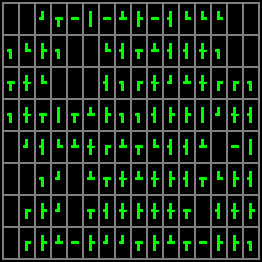
\includegraphics[scale=0.75]{\CURPATH/shuffled.png}
\caption{Разобранная головоломка}
\end{figure}

\dots и собранная:

\begin{figure}[H]
\label{fig:pipe_solved}
\centering
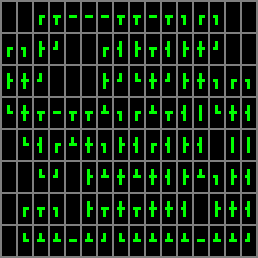
\includegraphics[scale=0.75]{\CURPATH/solved.png}
\caption{Собранная головоломка}
\end{figure}

Попробуем найти способ собрать её.

\subsubsection{Создание}

В начале, нужно её создать.
Вот простая идея.
Возьем массив ячеек 8*16.
Каждая ячейка может содержать какой-то тип блока.
Между ячейками есть стыки:

\pgfmathsetmacro\Width{16}
\pgfmathsetmacro\Height{8}
%\pgfmathsetmacro\Width{10}
%\pgfmathsetmacro\Height{5}
\pgfmathtruncatemacro\WidthMinusI{\Width - 1}
\pgfmathtruncatemacro\WidthMinusII{\Width - 2}
\pgfmathtruncatemacro\HeightMinusI{\Height - 1}
\pgfmathtruncatemacro\HeightMinusII{\Height - 2}
\pgfmathtruncatemacro\HeightPlusII{\Height + 2}
\pgfmathsetmacro\HeightPlusIi{\Height + 1.5}

% see also: http://www.texample.net/tikz/examples/euclid-algorithm/
\begin{center}
\begin{tikzpicture}[set style={{help lines}+=[dashed]},scale=0.7]

	\draw[style=help lines] (0,0) grid +(\Width,\Height);

	\foreach \c in {0,...,\WidthMinusI}
	{
		\foreach \r in {0,...,\HeightMinusII}
			\draw   [red,very thick,-] (\c+0.5,\r+0.75) -- (\c+0.5,\r+1.25);
		%\node[rotate=90] at (\c+0.5,\HeightPlusII) {\Large vjoints[\dots, \c] \normalsize};
		\node[rotate=90] at (\c+0.5,\HeightPlusII) {vjoints[\dots, \c]};
	}

	\foreach \r in {0,...,\HeightMinusI}
	{
		\foreach \c in {0,...,\WidthMinusII}
			\draw   [blue,very thick,-] (\c+0.75,\r+0.5) -- (\c+1.25,\r+0.5);
		\pgfmathtruncatemacro\hjointslabel{\HeightMinusI - \r}
		%\node at (-1.5,\r+0.5) {\large hjoints[\hjointslabel, \dots] \normalsize};
		\node at (-1.5,\r+0.5) {hjoints[\hjointslabel, \dots]};
	}

\end{tikzpicture}
\end{center}



Синие линии это горизонтальные стыки, красные линии это вертикальные стыки.
Мы просто случайно выставляем каждый стык в 0/false (отсутствует) или 1/true (присутствует).

После этого, теперь легко найти тип каждой ячейки.
А это:

\newcommand{\HeaderColor}{\cellcolor{blue!25}}
\begin{center}
\begin{longtable}{ | l | l | l | l | }
\hline
\HeaderColor стыки & \HeaderColor наше внутреннее название & \HeaderColor угол & \HeaderColor символ \\
\hline
0	&type 0		&	0$^{\circ}$	& (пробел)	\\
2	&type 2a	&	0$^{\circ}$	& \pmboxdrawuni{2503} \\ % ┃
2	&type 2a	&	90$^{\circ}$	& \pmboxdrawuni{2501} \\ % ━
2	&type 2b	&	0$^{\circ}$	& \pmboxdrawuni{250F} \\ % ┏
2	&type 2b	&	90$^{\circ}$	& \pmboxdrawuni{2513} \\ % ┓
2	&type 2b	&	180$^{\circ}$	& \pmboxdrawuni{251B} \\ % ┛
2	&type 2b	&	270$^{\circ}$	& \pmboxdrawuni{2517} \\ % ┗
3	&type 3		&	0$^{\circ}$	& \pmboxdrawuni{2523} \\ % ┣
3 	&type 3		&	90$^{\circ}$	& \pmboxdrawuni{2533} \\ % ┳
3	&type 3		&	180$^{\circ}$	& \pmboxdrawuni{252B} \\ % ┫
3	&type 3		&	270$^{\circ}$	& \pmboxdrawuni{253B} \\ % ┻
4	&type 4		&	0$^{\circ}$	& \pmboxdrawuni{254B} \\ % ╋
\hline
\end{longtable}
\end{center}

\textit{Висящие} стыки могут присутствовать на первой стадии (т.е., ячейки только с одним стыком), но они удалются
рекурсивно, и эти ячейки преобразуются в пустые ячейки.
Так что, в самом конце, все ячейки имеют минимум 2 стыка, и вся эта сантехническая система не имеет связей с внешним миром ---
я надеюсь, из-за этого станет немного проще.

Исходник генератора на Си здесь: \url{.../pipe/generator}.
Все вертикальные стыки хранятся в глобальном массиве \textit{hjoints[]} и вертикальные в \textit{vjoints[]}.

Программа на Си генерирует ANSI-раскрашенный вывод, как это было показано выше
(\ref{fig:pipe_shuffled}, \ref{fig:pipe_solved}) плюс массив типов для каждой ячейки, но без информации об углах:

\begin{lstlisting}[label=init_cells]
[
["0", "0", "2b", "3", "2a", "2a", "2a", "3", "3", "2a", "3", "2b", "2b", "2b", "0", "0"],
["2b", "2b", "3", "2b", "0", "0", "2b", "3", "3", "3", "3", "3", "4", "2b", "0", "0"],
["3", "4", "2b", "0", "0", "0", "3", "2b", "2b", "4", "2b", "3", "4", "2b", "2b", "2b"],
["2b", "4", "3", "2a", "3", "3", "3", "2b", "2b", "3", "3", "3", "2a", "2b", "4", "3"],
["0", "2b", "3", "2b", "3", "4", "2b", "3", "3", "2b", "3", "3", "3", "0", "2a", "2a"],
["0", "0", "2b", "2b", "0", "3", "3", "4", "3", "4", "3", "3", "3", "2b", "3", "3"],
["0", "2b", "3", "2b", "0", "3", "3", "4", "3", "4", "4", "3", "0", "3", "4", "3"],
["0", "2b", "3", "3", "2a", "3", "2b", "2b", "3", "3", "3", "3", "2a", "3", "3", "2b"],
]
\end{lstlisting}

\subsubsection{Решение}

Прежде всего, мы будем работать с массивом ячеек 8*16, где каждый элемент имеет 4 бита:
``T'' (top/верх),
``B'' (bottom/низ),
``L'' (left/лево),
``R'' (right/право).
Каждый бит представляет собой половину стыка.

% see also: http://www.texample.net/tikz/examples/euclid-algorithm/
\begin{center}
\begin{tikzpicture}[set style={{help lines}+=[dashed]},scale=0.7]

	\draw[style=help lines] (0,0) grid +(\Width,\Height);
	
	\foreach \c in {0,...,\WidthMinusI}
		%\node[rotate=90] at (\c+0.5,\HeightPlusIi) {\Large [\dots, \c] \normalsize};
		\node[rotate=90] at (\c+0.5,\HeightPlusIi) {[\dots, \c]};
	
	\foreach \r in {0,...,\HeightMinusI}
	{
		\pgfmathtruncatemacro\hlabel{\HeightMinusI - \r}
		%\node at (-1.5,\r+0.5) {\large [\hlabel, \dots] \normalsize};
		\node at (-1.5,\r+0.5) {[\hlabel, \dots]};
	
		\pgfmathsetmacro\Shift{0.325}
		\foreach \c in {0,...,\WidthMinusI}
		{
			\node at (\c+0.5,\r+0.5 + \Shift) {\footnotesize T \normalsize};
			\node at (\c+0.5,\r+0.5 - \Shift) {\footnotesize B \normalsize};
			\node at (\c+0.5 - \Shift,\r+0.5) {\footnotesize L \normalsize};
			\node at (\c+0.5 + \Shift,\r+0.5) {\footnotesize R \normalsize};
		}
	}

\end{tikzpicture}
\end{center}


Теперь определяем массив для каждого из четырех полустыков + информация об угле:

\begin{lstlisting}
HEIGHT=8
WIDTH=16

# if T/B/R/L is Bool instead of Int, Z3 solver will work faster
T=[[Bool('cell_%d_%d_top' % (r, c)) for c in range(WIDTH)] for r in range(HEIGHT)]
B=[[Bool('cell_%d_%d_bottom' % (r, c)) for c in range(WIDTH)] for r in range(HEIGHT)]
R=[[Bool('cell_%d_%d_right' % (r, c)) for c in range(WIDTH)] for r in range(HEIGHT)]
L=[[Bool('cell_%d_%d_left' % (r, c)) for c in range(WIDTH)] for r in range(HEIGHT)]
A=[[Int('cell_%d_%d_angle' % (r, c)) for c in range(WIDTH)] for r in range(HEIGHT)]
\end{lstlisting}

Мы знаем, что если каждый из полустыков присутствует, ответный полустык также должен присутствовать, и наоборот. 
Определяем всё это используя эти констрайнты:

\begin{lstlisting}
# shorthand variables for True and False:
t=True
f=False

# "top" of each cell must be equal to "bottom" of the cell above
# "bottom" of each cell must be equal to "top" of the cell below
# "left" of each cell must be equal to "right" of the cell at left
# "right" of each cell must be equal to "left" of the cell at right
for r in range(HEIGHT):
    for c in range(WIDTH):
        if r!=0:
            s.add(T[r][c]==B[r-1][c])
        if r!=HEIGHT-1:
            s.add(B[r][c]==T[r+1][c])
        if c!=0:
            s.add(L[r][c]==R[r][c-1])
        if c!=WIDTH-1:
            s.add(R[r][c]==L[r][c+1])

# "left" of each cell of first column shouldn't have any connection
# so is "right" of each cell of the last column
for r in range(HEIGHT):
    s.add(L[r][0]==f)
    s.add(R[r][WIDTH-1]==f)

# "top" of each cell of the first row shouldn't have any connection
# so is "bottom" of each cell of the last row
for c in range(WIDTH):
    s.add(T[0][c]==f)
    s.add(B[HEIGHT-1][c]==f)
\end{lstlisting}

Теперь перебираем все ячейки в изначальном массиве (\ref{init_cells}).
Первые две ячейки здесь пустые. И третья имеет тип ``2b''.
Это ``\pmboxdrawuni{250F}'' % ┏
и его можно ориентировать четырьмя разными способами.
И если её угол это 0$^{\circ}$, верхний и правый полустыки присутствуют, остальные отсутствуют.
Если он имеет угол 90$^{\circ}$, он выглядит как 
``\pmboxdrawuni{2513}'', % ┓
и верхник и левый полустыки присутствуют, остальные отсутствуют.

На обычном русском языке: ``если ячейка этого типа имеет угол 0$^{\circ}$, вот эти полустыки должны присутствовать \textbf{ИЛИ}
если она имеет угол 90$^{\circ}$, эти полустыки должны присутствовать, \textbf{ИЛИ}, итд, итд.''

Точно также, мы определяем эти правила для всех типов и всех возможных углов:

\begin{lstlisting}
for r in range(HEIGHT):
    for c in range(WIDTH):
        ty=cells_type[r][c]

        if ty=="0":
            s.add(A[r][c]==f)
            s.add(T[r][c]==f, B[r][c]==f, L[r][c]==f, R[r][c]==f)

        if ty=="2a":
            s.add(Or(And(A[r][c]==0, L[r][c]==f, R[r][c]==f, T[r][c]==t, B[r][c]==t),   # §\pmboxdrawuni{2503}§
                    And(A[r][c]==90, L[r][c]==t, R[r][c]==t, T[r][c]==f, B[r][c]==f)))  # §\pmboxdrawuni{2501}§

        if ty=="2b":
            s.add(Or(And(A[r][c]==0, L[r][c]==f, R[r][c]==t, T[r][c]==f, B[r][c]==t),   # §\pmboxdrawuni{250F}§
                    And(A[r][c]==90, L[r][c]==t, R[r][c]==f, T[r][c]==f, B[r][c]==t),   # §\pmboxdrawuni{2513}§
                    And(A[r][c]==180, L[r][c]==t, R[r][c]==f, T[r][c]==t, B[r][c]==f),  # §\pmboxdrawuni{251B}§
                    And(A[r][c]==270, L[r][c]==f, R[r][c]==t, T[r][c]==t, B[r][c]==f))) # §\pmboxdrawuni{2517}§
	
        if ty=="3":
            s.add(Or(And(A[r][c]==0, L[r][c]==f, R[r][c]==t, T[r][c]==t, B[r][c]==t),   # §\pmboxdrawuni{2523}§
                    And(A[r][c]==90, L[r][c]==t, R[r][c]==t, T[r][c]==f, B[r][c]==t),   # §\pmboxdrawuni{2533}§
                    And(A[r][c]==180, L[r][c]==t, R[r][c]==f, T[r][c]==t, B[r][c]==t),  # §\pmboxdrawuni{252B}§
                    And(A[r][c]==270, L[r][c]==t, R[r][c]==t, T[r][c]==t, B[r][c]==f))) # §\pmboxdrawuni{253B}§

        if ty=="4":
            s.add(A[r][c]==0)
            s.add(T[r][c]==t, B[r][c]==t, L[r][c]==t, R[r][c]==t) # §\pmboxdrawuni{254B}§
\end{lstlisting}

Полный исходник здесь: \url{.../solver/solve_pipe_puzzle1.py}.

Получается такой результат (выводит угол для каждой ячейки и (псевдо)графическое представление):

\begin{figure}[H]
\centering
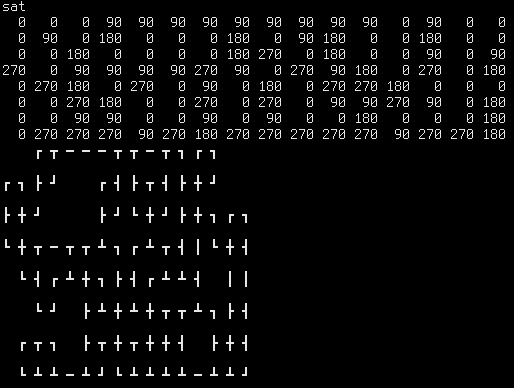
\includegraphics[scale=0.75]{\CURPATH/solver/solver.png}
\caption{Вывод скрипта солвера}
\end{figure}

Это работает $\approx 4$ секунды на моем старом и медленном Intel Atom N455 1.66GHz.
Быстро ли это? Не знаю, но снова вот что действительно круто, это то что мы понятия не имеем о какой-то математической
теории за всем этим, мы просто объявили ячейки, (полу-)стыки и определили отношения между ними.

Теперь следующий вопрос это, сколько здесь возможных решений?
Используя раннее описанный метод (\ref{SMTEnumerate}), я немного изменил скрипт солвера
\footnote{\url{.../solver/solve_pipe_puzzle2.py}} и солвер
сказал что возможно два решения.

Сравним их используя gvimdiff:

\begin{figure}[H]
\centering
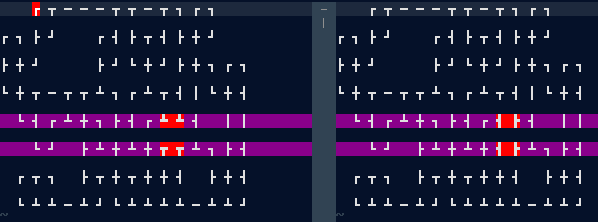
\includegraphics[scale=0.75]{\CURPATH/solver/diff.png}
\caption{Вывод gvimdiff (извините за мой красный курсор в левой части в левом верхнем углу)}
\end{figure}

4 ячейки в середине могут быть ориентированы по-разному.
Видимо, другие головоломки могут также выдавать разные результаты.

P.S.
\textit{Полу-стык} определен как булевый тип.
Но на самом деле, первая версия солвера была написана используя целочисленный тип для полу-стыков,
и 0 использовалось для False и 1 для True.
Я так сделал, потому что хотел более компактный исходный код, без использования длинных слов как ``False'' и ``True''.
И это работало, но медленнее. Вероятно, Z3 работает с булевыми типами быстрее? Лучше?
Так или иначе, я пишу это чтобы отметить, что, если нужно, целочисленный тип можно использовать вместо булевого.


\section{Развлекательная математика и головоломки}

\subsection{Судоку}

Головоломка Судоку это решетка 9*9, некоторые ячейки заполнены значениями, некоторые пустые:

% copypasted from http://www.texample.net/tikz/examples/sudoku/
\newcounter{row}
\newcounter{col}

\newcommand\setrow[9]{
  \setcounter{col}{1}
  \foreach \n in {#1, #2, #3, #4, #5, #6, #7, #8, #9} {
    \edef\x{\value{col} - 0.5}
    \edef\y{9.5 - \value{row}}
    \node[anchor=center] at (\x, \y) {\n};
    \stepcounter{col}
  }
  \stepcounter{row}
}

\begin{center}
\begin{tikzpicture}[scale=.7]
  \begin{scope}
    \draw (0, 0) grid (9, 9);
    \draw[very thick, scale=3] (0, 0) grid (3, 3);

    \setcounter{row}{1}
    \setrow { }{ }{5}  {3}{ }{ }  { }{ }{ }
    \setrow {8}{ }{ }  { }{ }{ }  { }{2}{ }
    \setrow { }{7}{ }  { }{1}{ }  {5}{ }{ }

    \setrow {4}{ }{ }  { }{ }{5}  {3}{ }{ }
    \setrow { }{1}{ }  { }{7}{ }  { }{ }{6}
    \setrow { }{ }{3}  {2}{ }{ }  { }{8}{ }

    \setrow { }{6}{ }  {5}{ }{ }  { }{ }{9}
    \setrow { }{ }{4}  { }{ }{ }  { }{3}{ }
    \setrow { }{ }{ }  { }{ }{9}  {7}{ }{ }

    \node[anchor=center] at (4.5, -0.5) {Нерешенная Судоку};
  \end{scope}
\end{tikzpicture}
\end{center}

Числа в каждом ряду должны быть уникальными, т.е., каждый ряд должен содержать 9 чисел в пределах 1..9 без повторений.
Та же история и для каждого столбца и каждого квадрата 3*3.

Головоломка представляет собой хороший кандидат, на котором можно попробовать \ac{SMT}-солвер, потому что это,
в общем-то, просто нерешенная система уравнений.

\input{puzzles/sudoku/1/main_RU}
%\input{puzzles/sudoku/GT/main_RU}
%\input{puzzles/sudoku/killer/main_RU}
\input{puzzles/sudoku/KLEE/main_RU}
\input{puzzles/sudoku/SAT/main_RU}


\subsection{Головоломка зебры (\ac{AKA} Загадка Эйнштейна)}

\input{puzzles/zebra/SMT/main_RU}
\input{puzzles/zebra/KLEE/main_RU}
\input{puzzles/zebra/SAT/main_RU}


\subsection{Решение головоломки ``трубы'' используя Z3 SMT-солвер}

\renewcommand{\CURPATH}{puzzles/pipe}

Головоломка ``трубы'' это популярная головоломка (просто погуглите ``pipe puzzle'' и посмотрите на картинки).

Вот как выглядит головоломка в разобранном виде:

\begin{figure}[H]
\label{fig:pipe_shuffled}
\centering
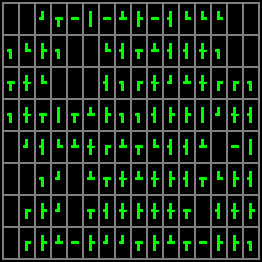
\includegraphics[scale=0.75]{\CURPATH/shuffled.png}
\caption{Разобранная головоломка}
\end{figure}

\dots и собранная:

\begin{figure}[H]
\label{fig:pipe_solved}
\centering
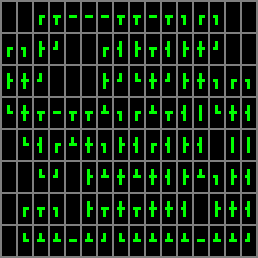
\includegraphics[scale=0.75]{\CURPATH/solved.png}
\caption{Собранная головоломка}
\end{figure}

Попробуем найти способ собрать её.

\subsubsection{Создание}

В начале, нужно её создать.
Вот простая идея.
Возьем массив ячеек 8*16.
Каждая ячейка может содержать какой-то тип блока.
Между ячейками есть стыки:

\input{\CURPATH/pipe_gen.tex}

Синие линии это горизонтальные стыки, красные линии это вертикальные стыки.
Мы просто случайно выставляем каждый стык в 0/false (отсутствует) или 1/true (присутствует).

После этого, теперь легко найти тип каждой ячейки.
А это:

\newcommand{\HeaderColor}{\cellcolor{blue!25}}
\begin{center}
\begin{longtable}{ | l | l | l | l | }
\hline
\HeaderColor стыки & \HeaderColor наше внутреннее название & \HeaderColor угол & \HeaderColor символ \\
\hline
0	&type 0		&	0$^{\circ}$	& (пробел)	\\
2	&type 2a	&	0$^{\circ}$	& \pmboxdrawuni{2503} \\ % ┃
2	&type 2a	&	90$^{\circ}$	& \pmboxdrawuni{2501} \\ % ━
2	&type 2b	&	0$^{\circ}$	& \pmboxdrawuni{250F} \\ % ┏
2	&type 2b	&	90$^{\circ}$	& \pmboxdrawuni{2513} \\ % ┓
2	&type 2b	&	180$^{\circ}$	& \pmboxdrawuni{251B} \\ % ┛
2	&type 2b	&	270$^{\circ}$	& \pmboxdrawuni{2517} \\ % ┗
3	&type 3		&	0$^{\circ}$	& \pmboxdrawuni{2523} \\ % ┣
3 	&type 3		&	90$^{\circ}$	& \pmboxdrawuni{2533} \\ % ┳
3	&type 3		&	180$^{\circ}$	& \pmboxdrawuni{252B} \\ % ┫
3	&type 3		&	270$^{\circ}$	& \pmboxdrawuni{253B} \\ % ┻
4	&type 4		&	0$^{\circ}$	& \pmboxdrawuni{254B} \\ % ╋
\hline
\end{longtable}
\end{center}

\textit{Висящие} стыки могут присутствовать на первой стадии (т.е., ячейки только с одним стыком), но они удалются
рекурсивно, и эти ячейки преобразуются в пустые ячейки.
Так что, в самом конце, все ячейки имеют минимум 2 стыка, и вся эта сантехническая система не имеет связей с внешним миром ---
я надеюсь, из-за этого станет немного проще.

Исходник генератора на Си здесь: \url{.../pipe/generator}.
Все вертикальные стыки хранятся в глобальном массиве \textit{hjoints[]} и вертикальные в \textit{vjoints[]}.

Программа на Си генерирует ANSI-раскрашенный вывод, как это было показано выше
(\ref{fig:pipe_shuffled}, \ref{fig:pipe_solved}) плюс массив типов для каждой ячейки, но без информации об углах:

\begin{lstlisting}[label=init_cells]
[
["0", "0", "2b", "3", "2a", "2a", "2a", "3", "3", "2a", "3", "2b", "2b", "2b", "0", "0"],
["2b", "2b", "3", "2b", "0", "0", "2b", "3", "3", "3", "3", "3", "4", "2b", "0", "0"],
["3", "4", "2b", "0", "0", "0", "3", "2b", "2b", "4", "2b", "3", "4", "2b", "2b", "2b"],
["2b", "4", "3", "2a", "3", "3", "3", "2b", "2b", "3", "3", "3", "2a", "2b", "4", "3"],
["0", "2b", "3", "2b", "3", "4", "2b", "3", "3", "2b", "3", "3", "3", "0", "2a", "2a"],
["0", "0", "2b", "2b", "0", "3", "3", "4", "3", "4", "3", "3", "3", "2b", "3", "3"],
["0", "2b", "3", "2b", "0", "3", "3", "4", "3", "4", "4", "3", "0", "3", "4", "3"],
["0", "2b", "3", "3", "2a", "3", "2b", "2b", "3", "3", "3", "3", "2a", "3", "3", "2b"],
]
\end{lstlisting}

\subsubsection{Решение}

Прежде всего, мы будем работать с массивом ячеек 8*16, где каждый элемент имеет 4 бита:
``T'' (top/верх),
``B'' (bottom/низ),
``L'' (left/лево),
``R'' (right/право).
Каждый бит представляет собой половину стыка.

\input{\CURPATH/pipe_solve.tex}

Теперь определяем массив для каждого из четырех полустыков + информация об угле:

\begin{lstlisting}
HEIGHT=8
WIDTH=16

# if T/B/R/L is Bool instead of Int, Z3 solver will work faster
T=[[Bool('cell_%d_%d_top' % (r, c)) for c in range(WIDTH)] for r in range(HEIGHT)]
B=[[Bool('cell_%d_%d_bottom' % (r, c)) for c in range(WIDTH)] for r in range(HEIGHT)]
R=[[Bool('cell_%d_%d_right' % (r, c)) for c in range(WIDTH)] for r in range(HEIGHT)]
L=[[Bool('cell_%d_%d_left' % (r, c)) for c in range(WIDTH)] for r in range(HEIGHT)]
A=[[Int('cell_%d_%d_angle' % (r, c)) for c in range(WIDTH)] for r in range(HEIGHT)]
\end{lstlisting}

Мы знаем, что если каждый из полустыков присутствует, ответный полустык также должен присутствовать, и наоборот. 
Определяем всё это используя эти констрайнты:

\begin{lstlisting}
# shorthand variables for True and False:
t=True
f=False

# "top" of each cell must be equal to "bottom" of the cell above
# "bottom" of each cell must be equal to "top" of the cell below
# "left" of each cell must be equal to "right" of the cell at left
# "right" of each cell must be equal to "left" of the cell at right
for r in range(HEIGHT):
    for c in range(WIDTH):
        if r!=0:
            s.add(T[r][c]==B[r-1][c])
        if r!=HEIGHT-1:
            s.add(B[r][c]==T[r+1][c])
        if c!=0:
            s.add(L[r][c]==R[r][c-1])
        if c!=WIDTH-1:
            s.add(R[r][c]==L[r][c+1])

# "left" of each cell of first column shouldn't have any connection
# so is "right" of each cell of the last column
for r in range(HEIGHT):
    s.add(L[r][0]==f)
    s.add(R[r][WIDTH-1]==f)

# "top" of each cell of the first row shouldn't have any connection
# so is "bottom" of each cell of the last row
for c in range(WIDTH):
    s.add(T[0][c]==f)
    s.add(B[HEIGHT-1][c]==f)
\end{lstlisting}

Теперь перебираем все ячейки в изначальном массиве (\ref{init_cells}).
Первые две ячейки здесь пустые. И третья имеет тип ``2b''.
Это ``\pmboxdrawuni{250F}'' % ┏
и его можно ориентировать четырьмя разными способами.
И если её угол это 0$^{\circ}$, верхний и правый полустыки присутствуют, остальные отсутствуют.
Если он имеет угол 90$^{\circ}$, он выглядит как 
``\pmboxdrawuni{2513}'', % ┓
и верхник и левый полустыки присутствуют, остальные отсутствуют.

На обычном русском языке: ``если ячейка этого типа имеет угол 0$^{\circ}$, вот эти полустыки должны присутствовать \textbf{ИЛИ}
если она имеет угол 90$^{\circ}$, эти полустыки должны присутствовать, \textbf{ИЛИ}, итд, итд.''

Точно также, мы определяем эти правила для всех типов и всех возможных углов:

\begin{lstlisting}
for r in range(HEIGHT):
    for c in range(WIDTH):
        ty=cells_type[r][c]

        if ty=="0":
            s.add(A[r][c]==f)
            s.add(T[r][c]==f, B[r][c]==f, L[r][c]==f, R[r][c]==f)

        if ty=="2a":
            s.add(Or(And(A[r][c]==0, L[r][c]==f, R[r][c]==f, T[r][c]==t, B[r][c]==t),   # §\pmboxdrawuni{2503}§
                    And(A[r][c]==90, L[r][c]==t, R[r][c]==t, T[r][c]==f, B[r][c]==f)))  # §\pmboxdrawuni{2501}§

        if ty=="2b":
            s.add(Or(And(A[r][c]==0, L[r][c]==f, R[r][c]==t, T[r][c]==f, B[r][c]==t),   # §\pmboxdrawuni{250F}§
                    And(A[r][c]==90, L[r][c]==t, R[r][c]==f, T[r][c]==f, B[r][c]==t),   # §\pmboxdrawuni{2513}§
                    And(A[r][c]==180, L[r][c]==t, R[r][c]==f, T[r][c]==t, B[r][c]==f),  # §\pmboxdrawuni{251B}§
                    And(A[r][c]==270, L[r][c]==f, R[r][c]==t, T[r][c]==t, B[r][c]==f))) # §\pmboxdrawuni{2517}§
	
        if ty=="3":
            s.add(Or(And(A[r][c]==0, L[r][c]==f, R[r][c]==t, T[r][c]==t, B[r][c]==t),   # §\pmboxdrawuni{2523}§
                    And(A[r][c]==90, L[r][c]==t, R[r][c]==t, T[r][c]==f, B[r][c]==t),   # §\pmboxdrawuni{2533}§
                    And(A[r][c]==180, L[r][c]==t, R[r][c]==f, T[r][c]==t, B[r][c]==t),  # §\pmboxdrawuni{252B}§
                    And(A[r][c]==270, L[r][c]==t, R[r][c]==t, T[r][c]==t, B[r][c]==f))) # §\pmboxdrawuni{253B}§

        if ty=="4":
            s.add(A[r][c]==0)
            s.add(T[r][c]==t, B[r][c]==t, L[r][c]==t, R[r][c]==t) # §\pmboxdrawuni{254B}§
\end{lstlisting}

Полный исходник здесь: \url{.../solver/solve_pipe_puzzle1.py}.

Получается такой результат (выводит угол для каждой ячейки и (псевдо)графическое представление):

\begin{figure}[H]
\centering
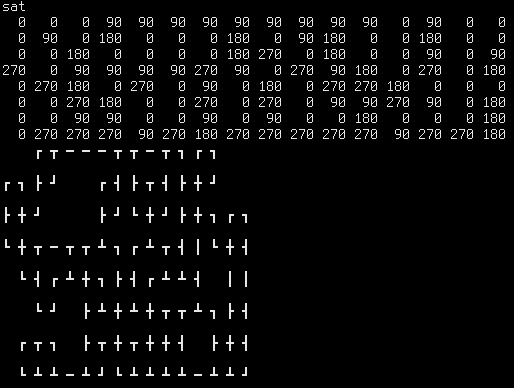
\includegraphics[scale=0.75]{\CURPATH/solver/solver.png}
\caption{Вывод скрипта солвера}
\end{figure}

Это работает $\approx 4$ секунды на моем старом и медленном Intel Atom N455 1.66GHz.
Быстро ли это? Не знаю, но снова вот что действительно круто, это то что мы понятия не имеем о какой-то математической
теории за всем этим, мы просто объявили ячейки, (полу-)стыки и определили отношения между ними.

Теперь следующий вопрос это, сколько здесь возможных решений?
Используя раннее описанный метод (\ref{SMTEnumerate}), я немного изменил скрипт солвера
\footnote{\url{.../solver/solve_pipe_puzzle2.py}} и солвер
сказал что возможно два решения.

Сравним их используя gvimdiff:

\begin{figure}[H]
\centering
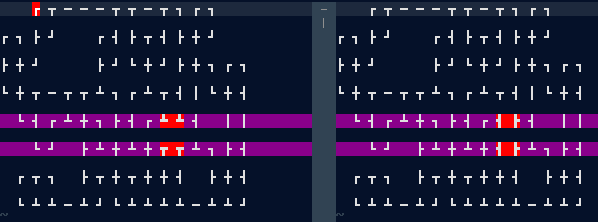
\includegraphics[scale=0.75]{\CURPATH/solver/diff.png}
\caption{Вывод gvimdiff (извините за мой красный курсор в левой части в левом верхнем углу)}
\end{figure}

4 ячейки в середине могут быть ориентированы по-разному.
Видимо, другие головоломки могут также выдавать разные результаты.

P.S.
\textit{Полу-стык} определен как булевый тип.
Но на самом деле, первая версия солвера была написана используя целочисленный тип для полу-стыков,
и 0 использовалось для False и 1 для True.
Я так сделал, потому что хотел более компактный исходный код, без использования длинных слов как ``False'' и ``True''.
И это работало, но медленнее. Вероятно, Z3 работает с булевыми типами быстрее? Лучше?
Так или иначе, я пишу это чтобы отметить, что, если нужно, целочисленный тип можно использовать вместо булевого.


\section{Развлекательная математика и головоломки}

\input{puzzles/sudoku/main_RU}
\input{puzzles/zebra/main_RU}
\input{puzzles/pipe/main_RU}
\input{puzzles/rubik2/failed_SMT/main_RU}
\input{puzzles/rubik2/SAT/main_RU}
\input{puzzles/rubik3/one_face_SMT/main_RU}
%\input{puzzles/numberlink/main_RU}
%\input{puzzles/two_parks_RU}
\input{puzzles/alphametics/main_RU}
%\input{puzzles/2015_AIME_II_Problems_12_RU}
%\input{puzzles/fred/main_RU}
%\input{puzzles/MC/main_RU}
%\input{puzzles/coin_flip/main_RU}
%\input{puzzles/Mock_AIME_2_2006-2007_Problem_8_RU}
%\input{puzzles/2012_AIME_I_Problems_1_RU}
%\input{puzzles/keypad_RU}


\section{Развлекательная математика и головоломки}

\input{puzzles/sudoku/main_RU}
\input{puzzles/zebra/main_RU}
\input{puzzles/pipe/main_RU}
\input{puzzles/rubik2/failed_SMT/main_RU}
\input{puzzles/rubik2/SAT/main_RU}
\input{puzzles/rubik3/one_face_SMT/main_RU}
%\input{puzzles/numberlink/main_RU}
%\input{puzzles/two_parks_RU}
\input{puzzles/alphametics/main_RU}
%\input{puzzles/2015_AIME_II_Problems_12_RU}
%\input{puzzles/fred/main_RU}
%\input{puzzles/MC/main_RU}
%\input{puzzles/coin_flip/main_RU}
%\input{puzzles/Mock_AIME_2_2006-2007_Problem_8_RU}
%\input{puzzles/2012_AIME_I_Problems_1_RU}
%\input{puzzles/keypad_RU}


\section{Развлекательная математика и головоломки}

\input{puzzles/sudoku/main_RU}
\input{puzzles/zebra/main_RU}
\input{puzzles/pipe/main_RU}
\input{puzzles/rubik2/failed_SMT/main_RU}
\input{puzzles/rubik2/SAT/main_RU}
\input{puzzles/rubik3/one_face_SMT/main_RU}
%\input{puzzles/numberlink/main_RU}
%\input{puzzles/two_parks_RU}
\input{puzzles/alphametics/main_RU}
%\input{puzzles/2015_AIME_II_Problems_12_RU}
%\input{puzzles/fred/main_RU}
%\input{puzzles/MC/main_RU}
%\input{puzzles/coin_flip/main_RU}
%\input{puzzles/Mock_AIME_2_2006-2007_Problem_8_RU}
%\input{puzzles/2012_AIME_I_Problems_1_RU}
%\input{puzzles/keypad_RU}


%\section{Развлекательная математика и головоломки}

\input{puzzles/sudoku/main_RU}
\input{puzzles/zebra/main_RU}
\input{puzzles/pipe/main_RU}
\input{puzzles/rubik2/failed_SMT/main_RU}
\input{puzzles/rubik2/SAT/main_RU}
\input{puzzles/rubik3/one_face_SMT/main_RU}
%\input{puzzles/numberlink/main_RU}
%\input{puzzles/two_parks_RU}
\input{puzzles/alphametics/main_RU}
%\input{puzzles/2015_AIME_II_Problems_12_RU}
%\input{puzzles/fred/main_RU}
%\input{puzzles/MC/main_RU}
%\input{puzzles/coin_flip/main_RU}
%\input{puzzles/Mock_AIME_2_2006-2007_Problem_8_RU}
%\input{puzzles/2012_AIME_I_Problems_1_RU}
%\input{puzzles/keypad_RU}


%\input{puzzles/two_parks_RU}
\subsection{Альфаметика}

Согласно Дональду Кнуту, термин ``Альфаметика'' был придуман Дж. Эйч. Аш. Хантером.
Это головоломка: какие десятичные цифры в пределах 0..9 нужно присвоить каждой букве, чтобы это уравнение было справедливо?

\begin{lstlisting}
  SEND
+ MORE
 -----
 MONEY
\end{lstlisting}

Для Z3 это легко:

\lstinputlisting{puzzles/alphametics/alpha.py}

Вывод:

\begin{lstlisting}
sat
[E, = 5,
 S, = 9,
 M, = 1,
 N, = 6,
 D, = 7,
 R, = 8,
 O, = 0,
 Y = 2]
\end{lstlisting}

Вот еще одна, из \ac{TAOCP} том IV (\url{http://www-cs-faculty.stanford.edu/~uno/fasc2b.ps.gz}):

\lstinputlisting{puzzles/alphametics/alpha2.py}

\begin{lstlisting}
sat
[L, = 6,
 S, = 7,
 N, = 2,
 T, = 1,
 I, = 5,
 V = 3,
 A, = 8,
 R, = 9,
 O, = 4,
 TRIO = 1954,
 SONATA, = 742818,
 VIOLA, = 35468,
 VIOLIN, = 354652]
\end{lstlisting}

% TODO URL
Эту головоломку я нашел в примерах pySMT:

\lstinputlisting{puzzles/alphametics/alpha3.py}

\begin{lstlisting}
sat
[D = 5, R = 4, O = 3, E = 8, L = 6, W = 7, H = 2]
\end{lstlisting}

%%% 

Это упражнение Q209 из
[Companion to the Papers of Donald Knuth]\footnote{\url{http://www-cs-faculty.stanford.edu/~knuth/cp.html}}.

\begin{lstlisting}
 KNIFE
  FORK
 SPOON
  SOUP
------
SUPPER
\end{lstlisting}

В целях упрощения, я добавил ф-цию (list\_to\_expr()):

\lstinputlisting{puzzles/alphametics/alpha4.py}

\begin{lstlisting}
sat
[K = 7,
 N = 4,
 R = 9,
 I = 1,
 E = 6,
 S = 0,
 O = 3,
 F = 5,
 U = 8,
 P = 2,
 SUPPER = 82269,
 SOUP = 382,
 SPOON = 2334,
 FORK = 5397,
 KNIFE = 74156]
\end{lstlisting}

S это 0, так что значение SUPPER начинается с (убранного) нуля. Скажем так, нам это не нравится.
Добавим это, чтобы это исправить:

\begin{lstlisting}
s.add(S!=0)
\end{lstlisting}

\begin{lstlisting}
sat
[K = 8,
 N = 4,
 R = 3,
 I = 7,
 E = 6,
 S = 1,
 O = 9,
 F = 2,
 U = 0,
 P = 5,
 SUPPER = 105563,
 SOUP = 1905,
 SPOON = 15994,
 FORK = 2938,
 KNIFE = 84726]
\end{lstlisting}

\paragraph{Создание своей собственной головоломки}

Вот проблема: есть только 10 букв, но как их выбрать из числа слов?
Мы можем использовать Z3 для этого:

\lstinputlisting{puzzles/alphametics/gen.py}

Это первая сгенерированная головоломка:

\begin{lstlisting}
sat
EGGS
JELLY
LUNCH
C 5
E 6
G 3
H 7
J 0
L 1
N 4
S 8
U 2
Y 9
\end{lstlisting}

Что если мы хотим, чтобы слово ``CAKE'' присутствовало в числе ``слагаемых''?

Добавим это:

\begin{lstlisting}
s.add(word_used[words.index('CAKE')])
\end{lstlisting}

\begin{lstlisting}
sat
CAKE
TEA
LUNCH
A 8
C 3
E 1
H 9
J 6
K 2
L 0
N 5
T 7
U 4
\end{lstlisting}

Добавим это:

\begin{lstlisting}
s.add(word_used[words.index('EGGS')])
\end{lstlisting}

Теперь оно может найти пару к EGGS:

\begin{lstlisting}
sat
EGGS
HONEY
LUNCH
C 6
E 7
G 9
H 4
L 5
N 8
O 2
S 3
U 0
Y 1
\end{lstlisting}

\paragraph{Файлы}

\url{https://github.com/DennisYurichev/...}




%\input{puzzles/2015_AIME_II_Problems_12_RU}
%\section{Развлекательная математика и головоломки}

\input{puzzles/sudoku/main_RU}
\input{puzzles/zebra/main_RU}
\input{puzzles/pipe/main_RU}
\input{puzzles/rubik2/failed_SMT/main_RU}
\input{puzzles/rubik2/SAT/main_RU}
\input{puzzles/rubik3/one_face_SMT/main_RU}
%\input{puzzles/numberlink/main_RU}
%\input{puzzles/two_parks_RU}
\input{puzzles/alphametics/main_RU}
%\input{puzzles/2015_AIME_II_Problems_12_RU}
%\input{puzzles/fred/main_RU}
%\input{puzzles/MC/main_RU}
%\input{puzzles/coin_flip/main_RU}
%\input{puzzles/Mock_AIME_2_2006-2007_Problem_8_RU}
%\input{puzzles/2012_AIME_I_Problems_1_RU}
%\input{puzzles/keypad_RU}


%\section{Развлекательная математика и головоломки}

\input{puzzles/sudoku/main_RU}
\input{puzzles/zebra/main_RU}
\input{puzzles/pipe/main_RU}
\input{puzzles/rubik2/failed_SMT/main_RU}
\input{puzzles/rubik2/SAT/main_RU}
\input{puzzles/rubik3/one_face_SMT/main_RU}
%\input{puzzles/numberlink/main_RU}
%\input{puzzles/two_parks_RU}
\input{puzzles/alphametics/main_RU}
%\input{puzzles/2015_AIME_II_Problems_12_RU}
%\input{puzzles/fred/main_RU}
%\input{puzzles/MC/main_RU}
%\input{puzzles/coin_flip/main_RU}
%\input{puzzles/Mock_AIME_2_2006-2007_Problem_8_RU}
%\input{puzzles/2012_AIME_I_Problems_1_RU}
%\input{puzzles/keypad_RU}


%\section{Развлекательная математика и головоломки}

\input{puzzles/sudoku/main_RU}
\input{puzzles/zebra/main_RU}
\input{puzzles/pipe/main_RU}
\input{puzzles/rubik2/failed_SMT/main_RU}
\input{puzzles/rubik2/SAT/main_RU}
\input{puzzles/rubik3/one_face_SMT/main_RU}
%\input{puzzles/numberlink/main_RU}
%\input{puzzles/two_parks_RU}
\input{puzzles/alphametics/main_RU}
%\input{puzzles/2015_AIME_II_Problems_12_RU}
%\input{puzzles/fred/main_RU}
%\input{puzzles/MC/main_RU}
%\input{puzzles/coin_flip/main_RU}
%\input{puzzles/Mock_AIME_2_2006-2007_Problem_8_RU}
%\input{puzzles/2012_AIME_I_Problems_1_RU}
%\input{puzzles/keypad_RU}


%\input{puzzles/Mock_AIME_2_2006-2007_Problem_8_RU}
%\input{puzzles/2012_AIME_I_Problems_1_RU}
%\input{puzzles/keypad_RU}


\section{Развлекательная математика и головоломки}

\subsection{Судоку}

Головоломка Судоку это решетка 9*9, некоторые ячейки заполнены значениями, некоторые пустые:

% copypasted from http://www.texample.net/tikz/examples/sudoku/
\newcounter{row}
\newcounter{col}

\newcommand\setrow[9]{
  \setcounter{col}{1}
  \foreach \n in {#1, #2, #3, #4, #5, #6, #7, #8, #9} {
    \edef\x{\value{col} - 0.5}
    \edef\y{9.5 - \value{row}}
    \node[anchor=center] at (\x, \y) {\n};
    \stepcounter{col}
  }
  \stepcounter{row}
}

\begin{center}
\begin{tikzpicture}[scale=.7]
  \begin{scope}
    \draw (0, 0) grid (9, 9);
    \draw[very thick, scale=3] (0, 0) grid (3, 3);

    \setcounter{row}{1}
    \setrow { }{ }{5}  {3}{ }{ }  { }{ }{ }
    \setrow {8}{ }{ }  { }{ }{ }  { }{2}{ }
    \setrow { }{7}{ }  { }{1}{ }  {5}{ }{ }

    \setrow {4}{ }{ }  { }{ }{5}  {3}{ }{ }
    \setrow { }{1}{ }  { }{7}{ }  { }{ }{6}
    \setrow { }{ }{3}  {2}{ }{ }  { }{8}{ }

    \setrow { }{6}{ }  {5}{ }{ }  { }{ }{9}
    \setrow { }{ }{4}  { }{ }{ }  { }{3}{ }
    \setrow { }{ }{ }  { }{ }{9}  {7}{ }{ }

    \node[anchor=center] at (4.5, -0.5) {Нерешенная Судоку};
  \end{scope}
\end{tikzpicture}
\end{center}

Числа в каждом ряду должны быть уникальными, т.е., каждый ряд должен содержать 9 чисел в пределах 1..9 без повторений.
Та же история и для каждого столбца и каждого квадрата 3*3.

Головоломка представляет собой хороший кандидат, на котором можно попробовать \ac{SMT}-солвер, потому что это,
в общем-то, просто нерешенная система уравнений.

\input{puzzles/sudoku/1/main_RU}
%\input{puzzles/sudoku/GT/main_RU}
%\input{puzzles/sudoku/killer/main_RU}
\input{puzzles/sudoku/KLEE/main_RU}
\input{puzzles/sudoku/SAT/main_RU}


\subsection{Головоломка зебры (\ac{AKA} Загадка Эйнштейна)}

\input{puzzles/zebra/SMT/main_RU}
\input{puzzles/zebra/KLEE/main_RU}
\input{puzzles/zebra/SAT/main_RU}


\subsection{Решение головоломки ``трубы'' используя Z3 SMT-солвер}

\renewcommand{\CURPATH}{puzzles/pipe}

Головоломка ``трубы'' это популярная головоломка (просто погуглите ``pipe puzzle'' и посмотрите на картинки).

Вот как выглядит головоломка в разобранном виде:

\begin{figure}[H]
\label{fig:pipe_shuffled}
\centering
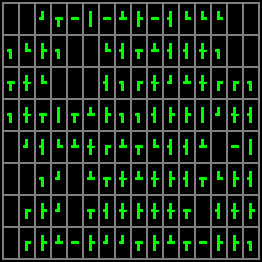
\includegraphics[scale=0.75]{\CURPATH/shuffled.png}
\caption{Разобранная головоломка}
\end{figure}

\dots и собранная:

\begin{figure}[H]
\label{fig:pipe_solved}
\centering
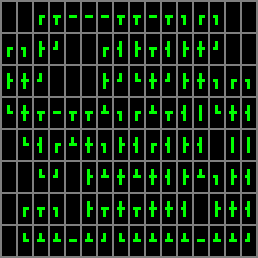
\includegraphics[scale=0.75]{\CURPATH/solved.png}
\caption{Собранная головоломка}
\end{figure}

Попробуем найти способ собрать её.

\subsubsection{Создание}

В начале, нужно её создать.
Вот простая идея.
Возьем массив ячеек 8*16.
Каждая ячейка может содержать какой-то тип блока.
Между ячейками есть стыки:

\input{\CURPATH/pipe_gen.tex}

Синие линии это горизонтальные стыки, красные линии это вертикальные стыки.
Мы просто случайно выставляем каждый стык в 0/false (отсутствует) или 1/true (присутствует).

После этого, теперь легко найти тип каждой ячейки.
А это:

\newcommand{\HeaderColor}{\cellcolor{blue!25}}
\begin{center}
\begin{longtable}{ | l | l | l | l | }
\hline
\HeaderColor стыки & \HeaderColor наше внутреннее название & \HeaderColor угол & \HeaderColor символ \\
\hline
0	&type 0		&	0$^{\circ}$	& (пробел)	\\
2	&type 2a	&	0$^{\circ}$	& \pmboxdrawuni{2503} \\ % ┃
2	&type 2a	&	90$^{\circ}$	& \pmboxdrawuni{2501} \\ % ━
2	&type 2b	&	0$^{\circ}$	& \pmboxdrawuni{250F} \\ % ┏
2	&type 2b	&	90$^{\circ}$	& \pmboxdrawuni{2513} \\ % ┓
2	&type 2b	&	180$^{\circ}$	& \pmboxdrawuni{251B} \\ % ┛
2	&type 2b	&	270$^{\circ}$	& \pmboxdrawuni{2517} \\ % ┗
3	&type 3		&	0$^{\circ}$	& \pmboxdrawuni{2523} \\ % ┣
3 	&type 3		&	90$^{\circ}$	& \pmboxdrawuni{2533} \\ % ┳
3	&type 3		&	180$^{\circ}$	& \pmboxdrawuni{252B} \\ % ┫
3	&type 3		&	270$^{\circ}$	& \pmboxdrawuni{253B} \\ % ┻
4	&type 4		&	0$^{\circ}$	& \pmboxdrawuni{254B} \\ % ╋
\hline
\end{longtable}
\end{center}

\textit{Висящие} стыки могут присутствовать на первой стадии (т.е., ячейки только с одним стыком), но они удалются
рекурсивно, и эти ячейки преобразуются в пустые ячейки.
Так что, в самом конце, все ячейки имеют минимум 2 стыка, и вся эта сантехническая система не имеет связей с внешним миром ---
я надеюсь, из-за этого станет немного проще.

Исходник генератора на Си здесь: \url{.../pipe/generator}.
Все вертикальные стыки хранятся в глобальном массиве \textit{hjoints[]} и вертикальные в \textit{vjoints[]}.

Программа на Си генерирует ANSI-раскрашенный вывод, как это было показано выше
(\ref{fig:pipe_shuffled}, \ref{fig:pipe_solved}) плюс массив типов для каждой ячейки, но без информации об углах:

\begin{lstlisting}[label=init_cells]
[
["0", "0", "2b", "3", "2a", "2a", "2a", "3", "3", "2a", "3", "2b", "2b", "2b", "0", "0"],
["2b", "2b", "3", "2b", "0", "0", "2b", "3", "3", "3", "3", "3", "4", "2b", "0", "0"],
["3", "4", "2b", "0", "0", "0", "3", "2b", "2b", "4", "2b", "3", "4", "2b", "2b", "2b"],
["2b", "4", "3", "2a", "3", "3", "3", "2b", "2b", "3", "3", "3", "2a", "2b", "4", "3"],
["0", "2b", "3", "2b", "3", "4", "2b", "3", "3", "2b", "3", "3", "3", "0", "2a", "2a"],
["0", "0", "2b", "2b", "0", "3", "3", "4", "3", "4", "3", "3", "3", "2b", "3", "3"],
["0", "2b", "3", "2b", "0", "3", "3", "4", "3", "4", "4", "3", "0", "3", "4", "3"],
["0", "2b", "3", "3", "2a", "3", "2b", "2b", "3", "3", "3", "3", "2a", "3", "3", "2b"],
]
\end{lstlisting}

\subsubsection{Решение}

Прежде всего, мы будем работать с массивом ячеек 8*16, где каждый элемент имеет 4 бита:
``T'' (top/верх),
``B'' (bottom/низ),
``L'' (left/лево),
``R'' (right/право).
Каждый бит представляет собой половину стыка.

\input{\CURPATH/pipe_solve.tex}

Теперь определяем массив для каждого из четырех полустыков + информация об угле:

\begin{lstlisting}
HEIGHT=8
WIDTH=16

# if T/B/R/L is Bool instead of Int, Z3 solver will work faster
T=[[Bool('cell_%d_%d_top' % (r, c)) for c in range(WIDTH)] for r in range(HEIGHT)]
B=[[Bool('cell_%d_%d_bottom' % (r, c)) for c in range(WIDTH)] for r in range(HEIGHT)]
R=[[Bool('cell_%d_%d_right' % (r, c)) for c in range(WIDTH)] for r in range(HEIGHT)]
L=[[Bool('cell_%d_%d_left' % (r, c)) for c in range(WIDTH)] for r in range(HEIGHT)]
A=[[Int('cell_%d_%d_angle' % (r, c)) for c in range(WIDTH)] for r in range(HEIGHT)]
\end{lstlisting}

Мы знаем, что если каждый из полустыков присутствует, ответный полустык также должен присутствовать, и наоборот. 
Определяем всё это используя эти констрайнты:

\begin{lstlisting}
# shorthand variables for True and False:
t=True
f=False

# "top" of each cell must be equal to "bottom" of the cell above
# "bottom" of each cell must be equal to "top" of the cell below
# "left" of each cell must be equal to "right" of the cell at left
# "right" of each cell must be equal to "left" of the cell at right
for r in range(HEIGHT):
    for c in range(WIDTH):
        if r!=0:
            s.add(T[r][c]==B[r-1][c])
        if r!=HEIGHT-1:
            s.add(B[r][c]==T[r+1][c])
        if c!=0:
            s.add(L[r][c]==R[r][c-1])
        if c!=WIDTH-1:
            s.add(R[r][c]==L[r][c+1])

# "left" of each cell of first column shouldn't have any connection
# so is "right" of each cell of the last column
for r in range(HEIGHT):
    s.add(L[r][0]==f)
    s.add(R[r][WIDTH-1]==f)

# "top" of each cell of the first row shouldn't have any connection
# so is "bottom" of each cell of the last row
for c in range(WIDTH):
    s.add(T[0][c]==f)
    s.add(B[HEIGHT-1][c]==f)
\end{lstlisting}

Теперь перебираем все ячейки в изначальном массиве (\ref{init_cells}).
Первые две ячейки здесь пустые. И третья имеет тип ``2b''.
Это ``\pmboxdrawuni{250F}'' % ┏
и его можно ориентировать четырьмя разными способами.
И если её угол это 0$^{\circ}$, верхний и правый полустыки присутствуют, остальные отсутствуют.
Если он имеет угол 90$^{\circ}$, он выглядит как 
``\pmboxdrawuni{2513}'', % ┓
и верхник и левый полустыки присутствуют, остальные отсутствуют.

На обычном русском языке: ``если ячейка этого типа имеет угол 0$^{\circ}$, вот эти полустыки должны присутствовать \textbf{ИЛИ}
если она имеет угол 90$^{\circ}$, эти полустыки должны присутствовать, \textbf{ИЛИ}, итд, итд.''

Точно также, мы определяем эти правила для всех типов и всех возможных углов:

\begin{lstlisting}
for r in range(HEIGHT):
    for c in range(WIDTH):
        ty=cells_type[r][c]

        if ty=="0":
            s.add(A[r][c]==f)
            s.add(T[r][c]==f, B[r][c]==f, L[r][c]==f, R[r][c]==f)

        if ty=="2a":
            s.add(Or(And(A[r][c]==0, L[r][c]==f, R[r][c]==f, T[r][c]==t, B[r][c]==t),   # §\pmboxdrawuni{2503}§
                    And(A[r][c]==90, L[r][c]==t, R[r][c]==t, T[r][c]==f, B[r][c]==f)))  # §\pmboxdrawuni{2501}§

        if ty=="2b":
            s.add(Or(And(A[r][c]==0, L[r][c]==f, R[r][c]==t, T[r][c]==f, B[r][c]==t),   # §\pmboxdrawuni{250F}§
                    And(A[r][c]==90, L[r][c]==t, R[r][c]==f, T[r][c]==f, B[r][c]==t),   # §\pmboxdrawuni{2513}§
                    And(A[r][c]==180, L[r][c]==t, R[r][c]==f, T[r][c]==t, B[r][c]==f),  # §\pmboxdrawuni{251B}§
                    And(A[r][c]==270, L[r][c]==f, R[r][c]==t, T[r][c]==t, B[r][c]==f))) # §\pmboxdrawuni{2517}§
	
        if ty=="3":
            s.add(Or(And(A[r][c]==0, L[r][c]==f, R[r][c]==t, T[r][c]==t, B[r][c]==t),   # §\pmboxdrawuni{2523}§
                    And(A[r][c]==90, L[r][c]==t, R[r][c]==t, T[r][c]==f, B[r][c]==t),   # §\pmboxdrawuni{2533}§
                    And(A[r][c]==180, L[r][c]==t, R[r][c]==f, T[r][c]==t, B[r][c]==t),  # §\pmboxdrawuni{252B}§
                    And(A[r][c]==270, L[r][c]==t, R[r][c]==t, T[r][c]==t, B[r][c]==f))) # §\pmboxdrawuni{253B}§

        if ty=="4":
            s.add(A[r][c]==0)
            s.add(T[r][c]==t, B[r][c]==t, L[r][c]==t, R[r][c]==t) # §\pmboxdrawuni{254B}§
\end{lstlisting}

Полный исходник здесь: \url{.../solver/solve_pipe_puzzle1.py}.

Получается такой результат (выводит угол для каждой ячейки и (псевдо)графическое представление):

\begin{figure}[H]
\centering
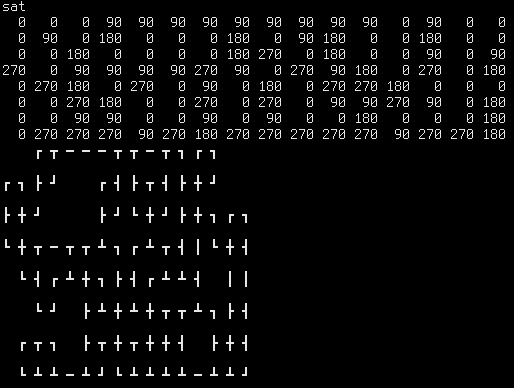
\includegraphics[scale=0.75]{\CURPATH/solver/solver.png}
\caption{Вывод скрипта солвера}
\end{figure}

Это работает $\approx 4$ секунды на моем старом и медленном Intel Atom N455 1.66GHz.
Быстро ли это? Не знаю, но снова вот что действительно круто, это то что мы понятия не имеем о какой-то математической
теории за всем этим, мы просто объявили ячейки, (полу-)стыки и определили отношения между ними.

Теперь следующий вопрос это, сколько здесь возможных решений?
Используя раннее описанный метод (\ref{SMTEnumerate}), я немного изменил скрипт солвера
\footnote{\url{.../solver/solve_pipe_puzzle2.py}} и солвер
сказал что возможно два решения.

Сравним их используя gvimdiff:

\begin{figure}[H]
\centering
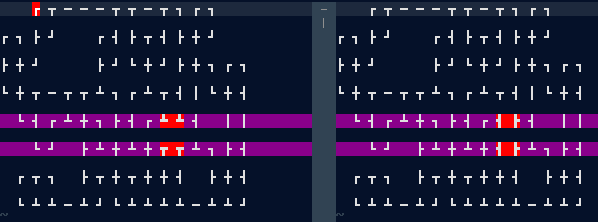
\includegraphics[scale=0.75]{\CURPATH/solver/diff.png}
\caption{Вывод gvimdiff (извините за мой красный курсор в левой части в левом верхнем углу)}
\end{figure}

4 ячейки в середине могут быть ориентированы по-разному.
Видимо, другие головоломки могут также выдавать разные результаты.

P.S.
\textit{Полу-стык} определен как булевый тип.
Но на самом деле, первая версия солвера была написана используя целочисленный тип для полу-стыков,
и 0 использовалось для False и 1 для True.
Я так сделал, потому что хотел более компактный исходный код, без использования длинных слов как ``False'' и ``True''.
И это работало, но медленнее. Вероятно, Z3 работает с булевыми типами быстрее? Лучше?
Так или иначе, я пишу это чтобы отметить, что, если нужно, целочисленный тип можно использовать вместо булевого.


\section{Развлекательная математика и головоломки}

\input{puzzles/sudoku/main_RU}
\input{puzzles/zebra/main_RU}
\input{puzzles/pipe/main_RU}
\input{puzzles/rubik2/failed_SMT/main_RU}
\input{puzzles/rubik2/SAT/main_RU}
\input{puzzles/rubik3/one_face_SMT/main_RU}
%\input{puzzles/numberlink/main_RU}
%\input{puzzles/two_parks_RU}
\input{puzzles/alphametics/main_RU}
%\input{puzzles/2015_AIME_II_Problems_12_RU}
%\input{puzzles/fred/main_RU}
%\input{puzzles/MC/main_RU}
%\input{puzzles/coin_flip/main_RU}
%\input{puzzles/Mock_AIME_2_2006-2007_Problem_8_RU}
%\input{puzzles/2012_AIME_I_Problems_1_RU}
%\input{puzzles/keypad_RU}


\section{Развлекательная математика и головоломки}

\input{puzzles/sudoku/main_RU}
\input{puzzles/zebra/main_RU}
\input{puzzles/pipe/main_RU}
\input{puzzles/rubik2/failed_SMT/main_RU}
\input{puzzles/rubik2/SAT/main_RU}
\input{puzzles/rubik3/one_face_SMT/main_RU}
%\input{puzzles/numberlink/main_RU}
%\input{puzzles/two_parks_RU}
\input{puzzles/alphametics/main_RU}
%\input{puzzles/2015_AIME_II_Problems_12_RU}
%\input{puzzles/fred/main_RU}
%\input{puzzles/MC/main_RU}
%\input{puzzles/coin_flip/main_RU}
%\input{puzzles/Mock_AIME_2_2006-2007_Problem_8_RU}
%\input{puzzles/2012_AIME_I_Problems_1_RU}
%\input{puzzles/keypad_RU}


\section{Развлекательная математика и головоломки}

\input{puzzles/sudoku/main_RU}
\input{puzzles/zebra/main_RU}
\input{puzzles/pipe/main_RU}
\input{puzzles/rubik2/failed_SMT/main_RU}
\input{puzzles/rubik2/SAT/main_RU}
\input{puzzles/rubik3/one_face_SMT/main_RU}
%\input{puzzles/numberlink/main_RU}
%\input{puzzles/two_parks_RU}
\input{puzzles/alphametics/main_RU}
%\input{puzzles/2015_AIME_II_Problems_12_RU}
%\input{puzzles/fred/main_RU}
%\input{puzzles/MC/main_RU}
%\input{puzzles/coin_flip/main_RU}
%\input{puzzles/Mock_AIME_2_2006-2007_Problem_8_RU}
%\input{puzzles/2012_AIME_I_Problems_1_RU}
%\input{puzzles/keypad_RU}


%\section{Развлекательная математика и головоломки}

\input{puzzles/sudoku/main_RU}
\input{puzzles/zebra/main_RU}
\input{puzzles/pipe/main_RU}
\input{puzzles/rubik2/failed_SMT/main_RU}
\input{puzzles/rubik2/SAT/main_RU}
\input{puzzles/rubik3/one_face_SMT/main_RU}
%\input{puzzles/numberlink/main_RU}
%\input{puzzles/two_parks_RU}
\input{puzzles/alphametics/main_RU}
%\input{puzzles/2015_AIME_II_Problems_12_RU}
%\input{puzzles/fred/main_RU}
%\input{puzzles/MC/main_RU}
%\input{puzzles/coin_flip/main_RU}
%\input{puzzles/Mock_AIME_2_2006-2007_Problem_8_RU}
%\input{puzzles/2012_AIME_I_Problems_1_RU}
%\input{puzzles/keypad_RU}


%\input{puzzles/two_parks_RU}
\subsection{Альфаметика}

Согласно Дональду Кнуту, термин ``Альфаметика'' был придуман Дж. Эйч. Аш. Хантером.
Это головоломка: какие десятичные цифры в пределах 0..9 нужно присвоить каждой букве, чтобы это уравнение было справедливо?

\begin{lstlisting}
  SEND
+ MORE
 -----
 MONEY
\end{lstlisting}

Для Z3 это легко:

\lstinputlisting{puzzles/alphametics/alpha.py}

Вывод:

\begin{lstlisting}
sat
[E, = 5,
 S, = 9,
 M, = 1,
 N, = 6,
 D, = 7,
 R, = 8,
 O, = 0,
 Y = 2]
\end{lstlisting}

Вот еще одна, из \ac{TAOCP} том IV (\url{http://www-cs-faculty.stanford.edu/~uno/fasc2b.ps.gz}):

\lstinputlisting{puzzles/alphametics/alpha2.py}

\begin{lstlisting}
sat
[L, = 6,
 S, = 7,
 N, = 2,
 T, = 1,
 I, = 5,
 V = 3,
 A, = 8,
 R, = 9,
 O, = 4,
 TRIO = 1954,
 SONATA, = 742818,
 VIOLA, = 35468,
 VIOLIN, = 354652]
\end{lstlisting}

% TODO URL
Эту головоломку я нашел в примерах pySMT:

\lstinputlisting{puzzles/alphametics/alpha3.py}

\begin{lstlisting}
sat
[D = 5, R = 4, O = 3, E = 8, L = 6, W = 7, H = 2]
\end{lstlisting}

%%% 

Это упражнение Q209 из
[Companion to the Papers of Donald Knuth]\footnote{\url{http://www-cs-faculty.stanford.edu/~knuth/cp.html}}.

\begin{lstlisting}
 KNIFE
  FORK
 SPOON
  SOUP
------
SUPPER
\end{lstlisting}

В целях упрощения, я добавил ф-цию (list\_to\_expr()):

\lstinputlisting{puzzles/alphametics/alpha4.py}

\begin{lstlisting}
sat
[K = 7,
 N = 4,
 R = 9,
 I = 1,
 E = 6,
 S = 0,
 O = 3,
 F = 5,
 U = 8,
 P = 2,
 SUPPER = 82269,
 SOUP = 382,
 SPOON = 2334,
 FORK = 5397,
 KNIFE = 74156]
\end{lstlisting}

S это 0, так что значение SUPPER начинается с (убранного) нуля. Скажем так, нам это не нравится.
Добавим это, чтобы это исправить:

\begin{lstlisting}
s.add(S!=0)
\end{lstlisting}

\begin{lstlisting}
sat
[K = 8,
 N = 4,
 R = 3,
 I = 7,
 E = 6,
 S = 1,
 O = 9,
 F = 2,
 U = 0,
 P = 5,
 SUPPER = 105563,
 SOUP = 1905,
 SPOON = 15994,
 FORK = 2938,
 KNIFE = 84726]
\end{lstlisting}

\paragraph{Создание своей собственной головоломки}

Вот проблема: есть только 10 букв, но как их выбрать из числа слов?
Мы можем использовать Z3 для этого:

\lstinputlisting{puzzles/alphametics/gen.py}

Это первая сгенерированная головоломка:

\begin{lstlisting}
sat
EGGS
JELLY
LUNCH
C 5
E 6
G 3
H 7
J 0
L 1
N 4
S 8
U 2
Y 9
\end{lstlisting}

Что если мы хотим, чтобы слово ``CAKE'' присутствовало в числе ``слагаемых''?

Добавим это:

\begin{lstlisting}
s.add(word_used[words.index('CAKE')])
\end{lstlisting}

\begin{lstlisting}
sat
CAKE
TEA
LUNCH
A 8
C 3
E 1
H 9
J 6
K 2
L 0
N 5
T 7
U 4
\end{lstlisting}

Добавим это:

\begin{lstlisting}
s.add(word_used[words.index('EGGS')])
\end{lstlisting}

Теперь оно может найти пару к EGGS:

\begin{lstlisting}
sat
EGGS
HONEY
LUNCH
C 6
E 7
G 9
H 4
L 5
N 8
O 2
S 3
U 0
Y 1
\end{lstlisting}

\paragraph{Файлы}

\url{https://github.com/DennisYurichev/...}




%\input{puzzles/2015_AIME_II_Problems_12_RU}
%\section{Развлекательная математика и головоломки}

\input{puzzles/sudoku/main_RU}
\input{puzzles/zebra/main_RU}
\input{puzzles/pipe/main_RU}
\input{puzzles/rubik2/failed_SMT/main_RU}
\input{puzzles/rubik2/SAT/main_RU}
\input{puzzles/rubik3/one_face_SMT/main_RU}
%\input{puzzles/numberlink/main_RU}
%\input{puzzles/two_parks_RU}
\input{puzzles/alphametics/main_RU}
%\input{puzzles/2015_AIME_II_Problems_12_RU}
%\input{puzzles/fred/main_RU}
%\input{puzzles/MC/main_RU}
%\input{puzzles/coin_flip/main_RU}
%\input{puzzles/Mock_AIME_2_2006-2007_Problem_8_RU}
%\input{puzzles/2012_AIME_I_Problems_1_RU}
%\input{puzzles/keypad_RU}


%\section{Развлекательная математика и головоломки}

\input{puzzles/sudoku/main_RU}
\input{puzzles/zebra/main_RU}
\input{puzzles/pipe/main_RU}
\input{puzzles/rubik2/failed_SMT/main_RU}
\input{puzzles/rubik2/SAT/main_RU}
\input{puzzles/rubik3/one_face_SMT/main_RU}
%\input{puzzles/numberlink/main_RU}
%\input{puzzles/two_parks_RU}
\input{puzzles/alphametics/main_RU}
%\input{puzzles/2015_AIME_II_Problems_12_RU}
%\input{puzzles/fred/main_RU}
%\input{puzzles/MC/main_RU}
%\input{puzzles/coin_flip/main_RU}
%\input{puzzles/Mock_AIME_2_2006-2007_Problem_8_RU}
%\input{puzzles/2012_AIME_I_Problems_1_RU}
%\input{puzzles/keypad_RU}


%\section{Развлекательная математика и головоломки}

\input{puzzles/sudoku/main_RU}
\input{puzzles/zebra/main_RU}
\input{puzzles/pipe/main_RU}
\input{puzzles/rubik2/failed_SMT/main_RU}
\input{puzzles/rubik2/SAT/main_RU}
\input{puzzles/rubik3/one_face_SMT/main_RU}
%\input{puzzles/numberlink/main_RU}
%\input{puzzles/two_parks_RU}
\input{puzzles/alphametics/main_RU}
%\input{puzzles/2015_AIME_II_Problems_12_RU}
%\input{puzzles/fred/main_RU}
%\input{puzzles/MC/main_RU}
%\input{puzzles/coin_flip/main_RU}
%\input{puzzles/Mock_AIME_2_2006-2007_Problem_8_RU}
%\input{puzzles/2012_AIME_I_Problems_1_RU}
%\input{puzzles/keypad_RU}


%\input{puzzles/Mock_AIME_2_2006-2007_Problem_8_RU}
%\input{puzzles/2012_AIME_I_Problems_1_RU}
%\input{puzzles/keypad_RU}


\section{Развлекательная математика и головоломки}

\subsection{Судоку}

Головоломка Судоку это решетка 9*9, некоторые ячейки заполнены значениями, некоторые пустые:

% copypasted from http://www.texample.net/tikz/examples/sudoku/
\newcounter{row}
\newcounter{col}

\newcommand\setrow[9]{
  \setcounter{col}{1}
  \foreach \n in {#1, #2, #3, #4, #5, #6, #7, #8, #9} {
    \edef\x{\value{col} - 0.5}
    \edef\y{9.5 - \value{row}}
    \node[anchor=center] at (\x, \y) {\n};
    \stepcounter{col}
  }
  \stepcounter{row}
}

\begin{center}
\begin{tikzpicture}[scale=.7]
  \begin{scope}
    \draw (0, 0) grid (9, 9);
    \draw[very thick, scale=3] (0, 0) grid (3, 3);

    \setcounter{row}{1}
    \setrow { }{ }{5}  {3}{ }{ }  { }{ }{ }
    \setrow {8}{ }{ }  { }{ }{ }  { }{2}{ }
    \setrow { }{7}{ }  { }{1}{ }  {5}{ }{ }

    \setrow {4}{ }{ }  { }{ }{5}  {3}{ }{ }
    \setrow { }{1}{ }  { }{7}{ }  { }{ }{6}
    \setrow { }{ }{3}  {2}{ }{ }  { }{8}{ }

    \setrow { }{6}{ }  {5}{ }{ }  { }{ }{9}
    \setrow { }{ }{4}  { }{ }{ }  { }{3}{ }
    \setrow { }{ }{ }  { }{ }{9}  {7}{ }{ }

    \node[anchor=center] at (4.5, -0.5) {Нерешенная Судоку};
  \end{scope}
\end{tikzpicture}
\end{center}

Числа в каждом ряду должны быть уникальными, т.е., каждый ряд должен содержать 9 чисел в пределах 1..9 без повторений.
Та же история и для каждого столбца и каждого квадрата 3*3.

Головоломка представляет собой хороший кандидат, на котором можно попробовать \ac{SMT}-солвер, потому что это,
в общем-то, просто нерешенная система уравнений.

\input{puzzles/sudoku/1/main_RU}
%\input{puzzles/sudoku/GT/main_RU}
%\input{puzzles/sudoku/killer/main_RU}
\input{puzzles/sudoku/KLEE/main_RU}
\input{puzzles/sudoku/SAT/main_RU}


\subsection{Головоломка зебры (\ac{AKA} Загадка Эйнштейна)}

\input{puzzles/zebra/SMT/main_RU}
\input{puzzles/zebra/KLEE/main_RU}
\input{puzzles/zebra/SAT/main_RU}


\subsection{Решение головоломки ``трубы'' используя Z3 SMT-солвер}

\renewcommand{\CURPATH}{puzzles/pipe}

Головоломка ``трубы'' это популярная головоломка (просто погуглите ``pipe puzzle'' и посмотрите на картинки).

Вот как выглядит головоломка в разобранном виде:

\begin{figure}[H]
\label{fig:pipe_shuffled}
\centering
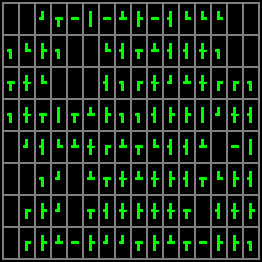
\includegraphics[scale=0.75]{\CURPATH/shuffled.png}
\caption{Разобранная головоломка}
\end{figure}

\dots и собранная:

\begin{figure}[H]
\label{fig:pipe_solved}
\centering
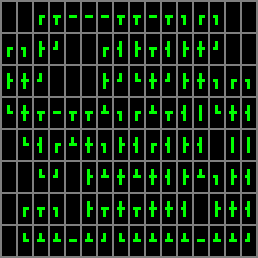
\includegraphics[scale=0.75]{\CURPATH/solved.png}
\caption{Собранная головоломка}
\end{figure}

Попробуем найти способ собрать её.

\subsubsection{Создание}

В начале, нужно её создать.
Вот простая идея.
Возьем массив ячеек 8*16.
Каждая ячейка может содержать какой-то тип блока.
Между ячейками есть стыки:

\input{\CURPATH/pipe_gen.tex}

Синие линии это горизонтальные стыки, красные линии это вертикальные стыки.
Мы просто случайно выставляем каждый стык в 0/false (отсутствует) или 1/true (присутствует).

После этого, теперь легко найти тип каждой ячейки.
А это:

\newcommand{\HeaderColor}{\cellcolor{blue!25}}
\begin{center}
\begin{longtable}{ | l | l | l | l | }
\hline
\HeaderColor стыки & \HeaderColor наше внутреннее название & \HeaderColor угол & \HeaderColor символ \\
\hline
0	&type 0		&	0$^{\circ}$	& (пробел)	\\
2	&type 2a	&	0$^{\circ}$	& \pmboxdrawuni{2503} \\ % ┃
2	&type 2a	&	90$^{\circ}$	& \pmboxdrawuni{2501} \\ % ━
2	&type 2b	&	0$^{\circ}$	& \pmboxdrawuni{250F} \\ % ┏
2	&type 2b	&	90$^{\circ}$	& \pmboxdrawuni{2513} \\ % ┓
2	&type 2b	&	180$^{\circ}$	& \pmboxdrawuni{251B} \\ % ┛
2	&type 2b	&	270$^{\circ}$	& \pmboxdrawuni{2517} \\ % ┗
3	&type 3		&	0$^{\circ}$	& \pmboxdrawuni{2523} \\ % ┣
3 	&type 3		&	90$^{\circ}$	& \pmboxdrawuni{2533} \\ % ┳
3	&type 3		&	180$^{\circ}$	& \pmboxdrawuni{252B} \\ % ┫
3	&type 3		&	270$^{\circ}$	& \pmboxdrawuni{253B} \\ % ┻
4	&type 4		&	0$^{\circ}$	& \pmboxdrawuni{254B} \\ % ╋
\hline
\end{longtable}
\end{center}

\textit{Висящие} стыки могут присутствовать на первой стадии (т.е., ячейки только с одним стыком), но они удалются
рекурсивно, и эти ячейки преобразуются в пустые ячейки.
Так что, в самом конце, все ячейки имеют минимум 2 стыка, и вся эта сантехническая система не имеет связей с внешним миром ---
я надеюсь, из-за этого станет немного проще.

Исходник генератора на Си здесь: \url{.../pipe/generator}.
Все вертикальные стыки хранятся в глобальном массиве \textit{hjoints[]} и вертикальные в \textit{vjoints[]}.

Программа на Си генерирует ANSI-раскрашенный вывод, как это было показано выше
(\ref{fig:pipe_shuffled}, \ref{fig:pipe_solved}) плюс массив типов для каждой ячейки, но без информации об углах:

\begin{lstlisting}[label=init_cells]
[
["0", "0", "2b", "3", "2a", "2a", "2a", "3", "3", "2a", "3", "2b", "2b", "2b", "0", "0"],
["2b", "2b", "3", "2b", "0", "0", "2b", "3", "3", "3", "3", "3", "4", "2b", "0", "0"],
["3", "4", "2b", "0", "0", "0", "3", "2b", "2b", "4", "2b", "3", "4", "2b", "2b", "2b"],
["2b", "4", "3", "2a", "3", "3", "3", "2b", "2b", "3", "3", "3", "2a", "2b", "4", "3"],
["0", "2b", "3", "2b", "3", "4", "2b", "3", "3", "2b", "3", "3", "3", "0", "2a", "2a"],
["0", "0", "2b", "2b", "0", "3", "3", "4", "3", "4", "3", "3", "3", "2b", "3", "3"],
["0", "2b", "3", "2b", "0", "3", "3", "4", "3", "4", "4", "3", "0", "3", "4", "3"],
["0", "2b", "3", "3", "2a", "3", "2b", "2b", "3", "3", "3", "3", "2a", "3", "3", "2b"],
]
\end{lstlisting}

\subsubsection{Решение}

Прежде всего, мы будем работать с массивом ячеек 8*16, где каждый элемент имеет 4 бита:
``T'' (top/верх),
``B'' (bottom/низ),
``L'' (left/лево),
``R'' (right/право).
Каждый бит представляет собой половину стыка.

\input{\CURPATH/pipe_solve.tex}

Теперь определяем массив для каждого из четырех полустыков + информация об угле:

\begin{lstlisting}
HEIGHT=8
WIDTH=16

# if T/B/R/L is Bool instead of Int, Z3 solver will work faster
T=[[Bool('cell_%d_%d_top' % (r, c)) for c in range(WIDTH)] for r in range(HEIGHT)]
B=[[Bool('cell_%d_%d_bottom' % (r, c)) for c in range(WIDTH)] for r in range(HEIGHT)]
R=[[Bool('cell_%d_%d_right' % (r, c)) for c in range(WIDTH)] for r in range(HEIGHT)]
L=[[Bool('cell_%d_%d_left' % (r, c)) for c in range(WIDTH)] for r in range(HEIGHT)]
A=[[Int('cell_%d_%d_angle' % (r, c)) for c in range(WIDTH)] for r in range(HEIGHT)]
\end{lstlisting}

Мы знаем, что если каждый из полустыков присутствует, ответный полустык также должен присутствовать, и наоборот. 
Определяем всё это используя эти констрайнты:

\begin{lstlisting}
# shorthand variables for True and False:
t=True
f=False

# "top" of each cell must be equal to "bottom" of the cell above
# "bottom" of each cell must be equal to "top" of the cell below
# "left" of each cell must be equal to "right" of the cell at left
# "right" of each cell must be equal to "left" of the cell at right
for r in range(HEIGHT):
    for c in range(WIDTH):
        if r!=0:
            s.add(T[r][c]==B[r-1][c])
        if r!=HEIGHT-1:
            s.add(B[r][c]==T[r+1][c])
        if c!=0:
            s.add(L[r][c]==R[r][c-1])
        if c!=WIDTH-1:
            s.add(R[r][c]==L[r][c+1])

# "left" of each cell of first column shouldn't have any connection
# so is "right" of each cell of the last column
for r in range(HEIGHT):
    s.add(L[r][0]==f)
    s.add(R[r][WIDTH-1]==f)

# "top" of each cell of the first row shouldn't have any connection
# so is "bottom" of each cell of the last row
for c in range(WIDTH):
    s.add(T[0][c]==f)
    s.add(B[HEIGHT-1][c]==f)
\end{lstlisting}

Теперь перебираем все ячейки в изначальном массиве (\ref{init_cells}).
Первые две ячейки здесь пустые. И третья имеет тип ``2b''.
Это ``\pmboxdrawuni{250F}'' % ┏
и его можно ориентировать четырьмя разными способами.
И если её угол это 0$^{\circ}$, верхний и правый полустыки присутствуют, остальные отсутствуют.
Если он имеет угол 90$^{\circ}$, он выглядит как 
``\pmboxdrawuni{2513}'', % ┓
и верхник и левый полустыки присутствуют, остальные отсутствуют.

На обычном русском языке: ``если ячейка этого типа имеет угол 0$^{\circ}$, вот эти полустыки должны присутствовать \textbf{ИЛИ}
если она имеет угол 90$^{\circ}$, эти полустыки должны присутствовать, \textbf{ИЛИ}, итд, итд.''

Точно также, мы определяем эти правила для всех типов и всех возможных углов:

\begin{lstlisting}
for r in range(HEIGHT):
    for c in range(WIDTH):
        ty=cells_type[r][c]

        if ty=="0":
            s.add(A[r][c]==f)
            s.add(T[r][c]==f, B[r][c]==f, L[r][c]==f, R[r][c]==f)

        if ty=="2a":
            s.add(Or(And(A[r][c]==0, L[r][c]==f, R[r][c]==f, T[r][c]==t, B[r][c]==t),   # §\pmboxdrawuni{2503}§
                    And(A[r][c]==90, L[r][c]==t, R[r][c]==t, T[r][c]==f, B[r][c]==f)))  # §\pmboxdrawuni{2501}§

        if ty=="2b":
            s.add(Or(And(A[r][c]==0, L[r][c]==f, R[r][c]==t, T[r][c]==f, B[r][c]==t),   # §\pmboxdrawuni{250F}§
                    And(A[r][c]==90, L[r][c]==t, R[r][c]==f, T[r][c]==f, B[r][c]==t),   # §\pmboxdrawuni{2513}§
                    And(A[r][c]==180, L[r][c]==t, R[r][c]==f, T[r][c]==t, B[r][c]==f),  # §\pmboxdrawuni{251B}§
                    And(A[r][c]==270, L[r][c]==f, R[r][c]==t, T[r][c]==t, B[r][c]==f))) # §\pmboxdrawuni{2517}§
	
        if ty=="3":
            s.add(Or(And(A[r][c]==0, L[r][c]==f, R[r][c]==t, T[r][c]==t, B[r][c]==t),   # §\pmboxdrawuni{2523}§
                    And(A[r][c]==90, L[r][c]==t, R[r][c]==t, T[r][c]==f, B[r][c]==t),   # §\pmboxdrawuni{2533}§
                    And(A[r][c]==180, L[r][c]==t, R[r][c]==f, T[r][c]==t, B[r][c]==t),  # §\pmboxdrawuni{252B}§
                    And(A[r][c]==270, L[r][c]==t, R[r][c]==t, T[r][c]==t, B[r][c]==f))) # §\pmboxdrawuni{253B}§

        if ty=="4":
            s.add(A[r][c]==0)
            s.add(T[r][c]==t, B[r][c]==t, L[r][c]==t, R[r][c]==t) # §\pmboxdrawuni{254B}§
\end{lstlisting}

Полный исходник здесь: \url{.../solver/solve_pipe_puzzle1.py}.

Получается такой результат (выводит угол для каждой ячейки и (псевдо)графическое представление):

\begin{figure}[H]
\centering
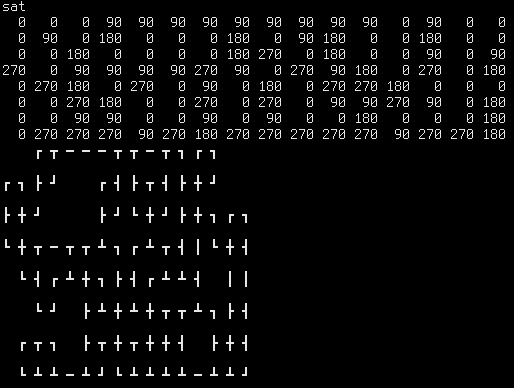
\includegraphics[scale=0.75]{\CURPATH/solver/solver.png}
\caption{Вывод скрипта солвера}
\end{figure}

Это работает $\approx 4$ секунды на моем старом и медленном Intel Atom N455 1.66GHz.
Быстро ли это? Не знаю, но снова вот что действительно круто, это то что мы понятия не имеем о какой-то математической
теории за всем этим, мы просто объявили ячейки, (полу-)стыки и определили отношения между ними.

Теперь следующий вопрос это, сколько здесь возможных решений?
Используя раннее описанный метод (\ref{SMTEnumerate}), я немного изменил скрипт солвера
\footnote{\url{.../solver/solve_pipe_puzzle2.py}} и солвер
сказал что возможно два решения.

Сравним их используя gvimdiff:

\begin{figure}[H]
\centering
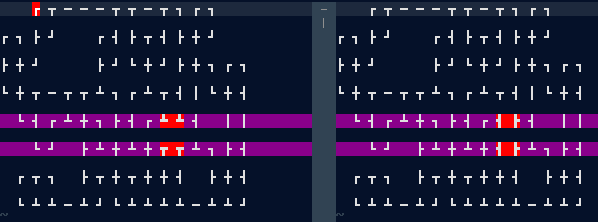
\includegraphics[scale=0.75]{\CURPATH/solver/diff.png}
\caption{Вывод gvimdiff (извините за мой красный курсор в левой части в левом верхнем углу)}
\end{figure}

4 ячейки в середине могут быть ориентированы по-разному.
Видимо, другие головоломки могут также выдавать разные результаты.

P.S.
\textit{Полу-стык} определен как булевый тип.
Но на самом деле, первая версия солвера была написана используя целочисленный тип для полу-стыков,
и 0 использовалось для False и 1 для True.
Я так сделал, потому что хотел более компактный исходный код, без использования длинных слов как ``False'' и ``True''.
И это работало, но медленнее. Вероятно, Z3 работает с булевыми типами быстрее? Лучше?
Так или иначе, я пишу это чтобы отметить, что, если нужно, целочисленный тип можно использовать вместо булевого.


\section{Развлекательная математика и головоломки}

\input{puzzles/sudoku/main_RU}
\input{puzzles/zebra/main_RU}
\input{puzzles/pipe/main_RU}
\input{puzzles/rubik2/failed_SMT/main_RU}
\input{puzzles/rubik2/SAT/main_RU}
\input{puzzles/rubik3/one_face_SMT/main_RU}
%\input{puzzles/numberlink/main_RU}
%\input{puzzles/two_parks_RU}
\input{puzzles/alphametics/main_RU}
%\input{puzzles/2015_AIME_II_Problems_12_RU}
%\input{puzzles/fred/main_RU}
%\input{puzzles/MC/main_RU}
%\input{puzzles/coin_flip/main_RU}
%\input{puzzles/Mock_AIME_2_2006-2007_Problem_8_RU}
%\input{puzzles/2012_AIME_I_Problems_1_RU}
%\input{puzzles/keypad_RU}


\section{Развлекательная математика и головоломки}

\input{puzzles/sudoku/main_RU}
\input{puzzles/zebra/main_RU}
\input{puzzles/pipe/main_RU}
\input{puzzles/rubik2/failed_SMT/main_RU}
\input{puzzles/rubik2/SAT/main_RU}
\input{puzzles/rubik3/one_face_SMT/main_RU}
%\input{puzzles/numberlink/main_RU}
%\input{puzzles/two_parks_RU}
\input{puzzles/alphametics/main_RU}
%\input{puzzles/2015_AIME_II_Problems_12_RU}
%\input{puzzles/fred/main_RU}
%\input{puzzles/MC/main_RU}
%\input{puzzles/coin_flip/main_RU}
%\input{puzzles/Mock_AIME_2_2006-2007_Problem_8_RU}
%\input{puzzles/2012_AIME_I_Problems_1_RU}
%\input{puzzles/keypad_RU}


\section{Развлекательная математика и головоломки}

\input{puzzles/sudoku/main_RU}
\input{puzzles/zebra/main_RU}
\input{puzzles/pipe/main_RU}
\input{puzzles/rubik2/failed_SMT/main_RU}
\input{puzzles/rubik2/SAT/main_RU}
\input{puzzles/rubik3/one_face_SMT/main_RU}
%\input{puzzles/numberlink/main_RU}
%\input{puzzles/two_parks_RU}
\input{puzzles/alphametics/main_RU}
%\input{puzzles/2015_AIME_II_Problems_12_RU}
%\input{puzzles/fred/main_RU}
%\input{puzzles/MC/main_RU}
%\input{puzzles/coin_flip/main_RU}
%\input{puzzles/Mock_AIME_2_2006-2007_Problem_8_RU}
%\input{puzzles/2012_AIME_I_Problems_1_RU}
%\input{puzzles/keypad_RU}


%\section{Развлекательная математика и головоломки}

\input{puzzles/sudoku/main_RU}
\input{puzzles/zebra/main_RU}
\input{puzzles/pipe/main_RU}
\input{puzzles/rubik2/failed_SMT/main_RU}
\input{puzzles/rubik2/SAT/main_RU}
\input{puzzles/rubik3/one_face_SMT/main_RU}
%\input{puzzles/numberlink/main_RU}
%\input{puzzles/two_parks_RU}
\input{puzzles/alphametics/main_RU}
%\input{puzzles/2015_AIME_II_Problems_12_RU}
%\input{puzzles/fred/main_RU}
%\input{puzzles/MC/main_RU}
%\input{puzzles/coin_flip/main_RU}
%\input{puzzles/Mock_AIME_2_2006-2007_Problem_8_RU}
%\input{puzzles/2012_AIME_I_Problems_1_RU}
%\input{puzzles/keypad_RU}


%\input{puzzles/two_parks_RU}
\subsection{Альфаметика}

Согласно Дональду Кнуту, термин ``Альфаметика'' был придуман Дж. Эйч. Аш. Хантером.
Это головоломка: какие десятичные цифры в пределах 0..9 нужно присвоить каждой букве, чтобы это уравнение было справедливо?

\begin{lstlisting}
  SEND
+ MORE
 -----
 MONEY
\end{lstlisting}

Для Z3 это легко:

\lstinputlisting{puzzles/alphametics/alpha.py}

Вывод:

\begin{lstlisting}
sat
[E, = 5,
 S, = 9,
 M, = 1,
 N, = 6,
 D, = 7,
 R, = 8,
 O, = 0,
 Y = 2]
\end{lstlisting}

Вот еще одна, из \ac{TAOCP} том IV (\url{http://www-cs-faculty.stanford.edu/~uno/fasc2b.ps.gz}):

\lstinputlisting{puzzles/alphametics/alpha2.py}

\begin{lstlisting}
sat
[L, = 6,
 S, = 7,
 N, = 2,
 T, = 1,
 I, = 5,
 V = 3,
 A, = 8,
 R, = 9,
 O, = 4,
 TRIO = 1954,
 SONATA, = 742818,
 VIOLA, = 35468,
 VIOLIN, = 354652]
\end{lstlisting}

% TODO URL
Эту головоломку я нашел в примерах pySMT:

\lstinputlisting{puzzles/alphametics/alpha3.py}

\begin{lstlisting}
sat
[D = 5, R = 4, O = 3, E = 8, L = 6, W = 7, H = 2]
\end{lstlisting}

%%% 

Это упражнение Q209 из
[Companion to the Papers of Donald Knuth]\footnote{\url{http://www-cs-faculty.stanford.edu/~knuth/cp.html}}.

\begin{lstlisting}
 KNIFE
  FORK
 SPOON
  SOUP
------
SUPPER
\end{lstlisting}

В целях упрощения, я добавил ф-цию (list\_to\_expr()):

\lstinputlisting{puzzles/alphametics/alpha4.py}

\begin{lstlisting}
sat
[K = 7,
 N = 4,
 R = 9,
 I = 1,
 E = 6,
 S = 0,
 O = 3,
 F = 5,
 U = 8,
 P = 2,
 SUPPER = 82269,
 SOUP = 382,
 SPOON = 2334,
 FORK = 5397,
 KNIFE = 74156]
\end{lstlisting}

S это 0, так что значение SUPPER начинается с (убранного) нуля. Скажем так, нам это не нравится.
Добавим это, чтобы это исправить:

\begin{lstlisting}
s.add(S!=0)
\end{lstlisting}

\begin{lstlisting}
sat
[K = 8,
 N = 4,
 R = 3,
 I = 7,
 E = 6,
 S = 1,
 O = 9,
 F = 2,
 U = 0,
 P = 5,
 SUPPER = 105563,
 SOUP = 1905,
 SPOON = 15994,
 FORK = 2938,
 KNIFE = 84726]
\end{lstlisting}

\paragraph{Создание своей собственной головоломки}

Вот проблема: есть только 10 букв, но как их выбрать из числа слов?
Мы можем использовать Z3 для этого:

\lstinputlisting{puzzles/alphametics/gen.py}

Это первая сгенерированная головоломка:

\begin{lstlisting}
sat
EGGS
JELLY
LUNCH
C 5
E 6
G 3
H 7
J 0
L 1
N 4
S 8
U 2
Y 9
\end{lstlisting}

Что если мы хотим, чтобы слово ``CAKE'' присутствовало в числе ``слагаемых''?

Добавим это:

\begin{lstlisting}
s.add(word_used[words.index('CAKE')])
\end{lstlisting}

\begin{lstlisting}
sat
CAKE
TEA
LUNCH
A 8
C 3
E 1
H 9
J 6
K 2
L 0
N 5
T 7
U 4
\end{lstlisting}

Добавим это:

\begin{lstlisting}
s.add(word_used[words.index('EGGS')])
\end{lstlisting}

Теперь оно может найти пару к EGGS:

\begin{lstlisting}
sat
EGGS
HONEY
LUNCH
C 6
E 7
G 9
H 4
L 5
N 8
O 2
S 3
U 0
Y 1
\end{lstlisting}

\paragraph{Файлы}

\url{https://github.com/DennisYurichev/...}




%\input{puzzles/2015_AIME_II_Problems_12_RU}
%\section{Развлекательная математика и головоломки}

\input{puzzles/sudoku/main_RU}
\input{puzzles/zebra/main_RU}
\input{puzzles/pipe/main_RU}
\input{puzzles/rubik2/failed_SMT/main_RU}
\input{puzzles/rubik2/SAT/main_RU}
\input{puzzles/rubik3/one_face_SMT/main_RU}
%\input{puzzles/numberlink/main_RU}
%\input{puzzles/two_parks_RU}
\input{puzzles/alphametics/main_RU}
%\input{puzzles/2015_AIME_II_Problems_12_RU}
%\input{puzzles/fred/main_RU}
%\input{puzzles/MC/main_RU}
%\input{puzzles/coin_flip/main_RU}
%\input{puzzles/Mock_AIME_2_2006-2007_Problem_8_RU}
%\input{puzzles/2012_AIME_I_Problems_1_RU}
%\input{puzzles/keypad_RU}


%\section{Развлекательная математика и головоломки}

\input{puzzles/sudoku/main_RU}
\input{puzzles/zebra/main_RU}
\input{puzzles/pipe/main_RU}
\input{puzzles/rubik2/failed_SMT/main_RU}
\input{puzzles/rubik2/SAT/main_RU}
\input{puzzles/rubik3/one_face_SMT/main_RU}
%\input{puzzles/numberlink/main_RU}
%\input{puzzles/two_parks_RU}
\input{puzzles/alphametics/main_RU}
%\input{puzzles/2015_AIME_II_Problems_12_RU}
%\input{puzzles/fred/main_RU}
%\input{puzzles/MC/main_RU}
%\input{puzzles/coin_flip/main_RU}
%\input{puzzles/Mock_AIME_2_2006-2007_Problem_8_RU}
%\input{puzzles/2012_AIME_I_Problems_1_RU}
%\input{puzzles/keypad_RU}


%\section{Развлекательная математика и головоломки}

\input{puzzles/sudoku/main_RU}
\input{puzzles/zebra/main_RU}
\input{puzzles/pipe/main_RU}
\input{puzzles/rubik2/failed_SMT/main_RU}
\input{puzzles/rubik2/SAT/main_RU}
\input{puzzles/rubik3/one_face_SMT/main_RU}
%\input{puzzles/numberlink/main_RU}
%\input{puzzles/two_parks_RU}
\input{puzzles/alphametics/main_RU}
%\input{puzzles/2015_AIME_II_Problems_12_RU}
%\input{puzzles/fred/main_RU}
%\input{puzzles/MC/main_RU}
%\input{puzzles/coin_flip/main_RU}
%\input{puzzles/Mock_AIME_2_2006-2007_Problem_8_RU}
%\input{puzzles/2012_AIME_I_Problems_1_RU}
%\input{puzzles/keypad_RU}


%\input{puzzles/Mock_AIME_2_2006-2007_Problem_8_RU}
%\input{puzzles/2012_AIME_I_Problems_1_RU}
%\input{puzzles/keypad_RU}


%\section{Развлекательная математика и головоломки}

\subsection{Судоку}

Головоломка Судоку это решетка 9*9, некоторые ячейки заполнены значениями, некоторые пустые:

% copypasted from http://www.texample.net/tikz/examples/sudoku/
\newcounter{row}
\newcounter{col}

\newcommand\setrow[9]{
  \setcounter{col}{1}
  \foreach \n in {#1, #2, #3, #4, #5, #6, #7, #8, #9} {
    \edef\x{\value{col} - 0.5}
    \edef\y{9.5 - \value{row}}
    \node[anchor=center] at (\x, \y) {\n};
    \stepcounter{col}
  }
  \stepcounter{row}
}

\begin{center}
\begin{tikzpicture}[scale=.7]
  \begin{scope}
    \draw (0, 0) grid (9, 9);
    \draw[very thick, scale=3] (0, 0) grid (3, 3);

    \setcounter{row}{1}
    \setrow { }{ }{5}  {3}{ }{ }  { }{ }{ }
    \setrow {8}{ }{ }  { }{ }{ }  { }{2}{ }
    \setrow { }{7}{ }  { }{1}{ }  {5}{ }{ }

    \setrow {4}{ }{ }  { }{ }{5}  {3}{ }{ }
    \setrow { }{1}{ }  { }{7}{ }  { }{ }{6}
    \setrow { }{ }{3}  {2}{ }{ }  { }{8}{ }

    \setrow { }{6}{ }  {5}{ }{ }  { }{ }{9}
    \setrow { }{ }{4}  { }{ }{ }  { }{3}{ }
    \setrow { }{ }{ }  { }{ }{9}  {7}{ }{ }

    \node[anchor=center] at (4.5, -0.5) {Нерешенная Судоку};
  \end{scope}
\end{tikzpicture}
\end{center}

Числа в каждом ряду должны быть уникальными, т.е., каждый ряд должен содержать 9 чисел в пределах 1..9 без повторений.
Та же история и для каждого столбца и каждого квадрата 3*3.

Головоломка представляет собой хороший кандидат, на котором можно попробовать \ac{SMT}-солвер, потому что это,
в общем-то, просто нерешенная система уравнений.

\input{puzzles/sudoku/1/main_RU}
%\input{puzzles/sudoku/GT/main_RU}
%\input{puzzles/sudoku/killer/main_RU}
\input{puzzles/sudoku/KLEE/main_RU}
\input{puzzles/sudoku/SAT/main_RU}


\subsection{Головоломка зебры (\ac{AKA} Загадка Эйнштейна)}

\input{puzzles/zebra/SMT/main_RU}
\input{puzzles/zebra/KLEE/main_RU}
\input{puzzles/zebra/SAT/main_RU}


\subsection{Решение головоломки ``трубы'' используя Z3 SMT-солвер}

\renewcommand{\CURPATH}{puzzles/pipe}

Головоломка ``трубы'' это популярная головоломка (просто погуглите ``pipe puzzle'' и посмотрите на картинки).

Вот как выглядит головоломка в разобранном виде:

\begin{figure}[H]
\label{fig:pipe_shuffled}
\centering
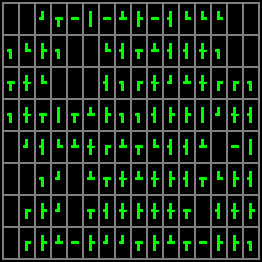
\includegraphics[scale=0.75]{\CURPATH/shuffled.png}
\caption{Разобранная головоломка}
\end{figure}

\dots и собранная:

\begin{figure}[H]
\label{fig:pipe_solved}
\centering
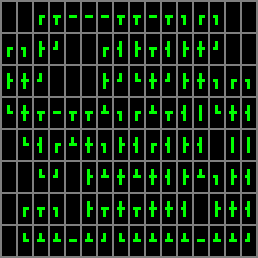
\includegraphics[scale=0.75]{\CURPATH/solved.png}
\caption{Собранная головоломка}
\end{figure}

Попробуем найти способ собрать её.

\subsubsection{Создание}

В начале, нужно её создать.
Вот простая идея.
Возьем массив ячеек 8*16.
Каждая ячейка может содержать какой-то тип блока.
Между ячейками есть стыки:

\input{\CURPATH/pipe_gen.tex}

Синие линии это горизонтальные стыки, красные линии это вертикальные стыки.
Мы просто случайно выставляем каждый стык в 0/false (отсутствует) или 1/true (присутствует).

После этого, теперь легко найти тип каждой ячейки.
А это:

\newcommand{\HeaderColor}{\cellcolor{blue!25}}
\begin{center}
\begin{longtable}{ | l | l | l | l | }
\hline
\HeaderColor стыки & \HeaderColor наше внутреннее название & \HeaderColor угол & \HeaderColor символ \\
\hline
0	&type 0		&	0$^{\circ}$	& (пробел)	\\
2	&type 2a	&	0$^{\circ}$	& \pmboxdrawuni{2503} \\ % ┃
2	&type 2a	&	90$^{\circ}$	& \pmboxdrawuni{2501} \\ % ━
2	&type 2b	&	0$^{\circ}$	& \pmboxdrawuni{250F} \\ % ┏
2	&type 2b	&	90$^{\circ}$	& \pmboxdrawuni{2513} \\ % ┓
2	&type 2b	&	180$^{\circ}$	& \pmboxdrawuni{251B} \\ % ┛
2	&type 2b	&	270$^{\circ}$	& \pmboxdrawuni{2517} \\ % ┗
3	&type 3		&	0$^{\circ}$	& \pmboxdrawuni{2523} \\ % ┣
3 	&type 3		&	90$^{\circ}$	& \pmboxdrawuni{2533} \\ % ┳
3	&type 3		&	180$^{\circ}$	& \pmboxdrawuni{252B} \\ % ┫
3	&type 3		&	270$^{\circ}$	& \pmboxdrawuni{253B} \\ % ┻
4	&type 4		&	0$^{\circ}$	& \pmboxdrawuni{254B} \\ % ╋
\hline
\end{longtable}
\end{center}

\textit{Висящие} стыки могут присутствовать на первой стадии (т.е., ячейки только с одним стыком), но они удалются
рекурсивно, и эти ячейки преобразуются в пустые ячейки.
Так что, в самом конце, все ячейки имеют минимум 2 стыка, и вся эта сантехническая система не имеет связей с внешним миром ---
я надеюсь, из-за этого станет немного проще.

Исходник генератора на Си здесь: \url{.../pipe/generator}.
Все вертикальные стыки хранятся в глобальном массиве \textit{hjoints[]} и вертикальные в \textit{vjoints[]}.

Программа на Си генерирует ANSI-раскрашенный вывод, как это было показано выше
(\ref{fig:pipe_shuffled}, \ref{fig:pipe_solved}) плюс массив типов для каждой ячейки, но без информации об углах:

\begin{lstlisting}[label=init_cells]
[
["0", "0", "2b", "3", "2a", "2a", "2a", "3", "3", "2a", "3", "2b", "2b", "2b", "0", "0"],
["2b", "2b", "3", "2b", "0", "0", "2b", "3", "3", "3", "3", "3", "4", "2b", "0", "0"],
["3", "4", "2b", "0", "0", "0", "3", "2b", "2b", "4", "2b", "3", "4", "2b", "2b", "2b"],
["2b", "4", "3", "2a", "3", "3", "3", "2b", "2b", "3", "3", "3", "2a", "2b", "4", "3"],
["0", "2b", "3", "2b", "3", "4", "2b", "3", "3", "2b", "3", "3", "3", "0", "2a", "2a"],
["0", "0", "2b", "2b", "0", "3", "3", "4", "3", "4", "3", "3", "3", "2b", "3", "3"],
["0", "2b", "3", "2b", "0", "3", "3", "4", "3", "4", "4", "3", "0", "3", "4", "3"],
["0", "2b", "3", "3", "2a", "3", "2b", "2b", "3", "3", "3", "3", "2a", "3", "3", "2b"],
]
\end{lstlisting}

\subsubsection{Решение}

Прежде всего, мы будем работать с массивом ячеек 8*16, где каждый элемент имеет 4 бита:
``T'' (top/верх),
``B'' (bottom/низ),
``L'' (left/лево),
``R'' (right/право).
Каждый бит представляет собой половину стыка.

\input{\CURPATH/pipe_solve.tex}

Теперь определяем массив для каждого из четырех полустыков + информация об угле:

\begin{lstlisting}
HEIGHT=8
WIDTH=16

# if T/B/R/L is Bool instead of Int, Z3 solver will work faster
T=[[Bool('cell_%d_%d_top' % (r, c)) for c in range(WIDTH)] for r in range(HEIGHT)]
B=[[Bool('cell_%d_%d_bottom' % (r, c)) for c in range(WIDTH)] for r in range(HEIGHT)]
R=[[Bool('cell_%d_%d_right' % (r, c)) for c in range(WIDTH)] for r in range(HEIGHT)]
L=[[Bool('cell_%d_%d_left' % (r, c)) for c in range(WIDTH)] for r in range(HEIGHT)]
A=[[Int('cell_%d_%d_angle' % (r, c)) for c in range(WIDTH)] for r in range(HEIGHT)]
\end{lstlisting}

Мы знаем, что если каждый из полустыков присутствует, ответный полустык также должен присутствовать, и наоборот. 
Определяем всё это используя эти констрайнты:

\begin{lstlisting}
# shorthand variables for True and False:
t=True
f=False

# "top" of each cell must be equal to "bottom" of the cell above
# "bottom" of each cell must be equal to "top" of the cell below
# "left" of each cell must be equal to "right" of the cell at left
# "right" of each cell must be equal to "left" of the cell at right
for r in range(HEIGHT):
    for c in range(WIDTH):
        if r!=0:
            s.add(T[r][c]==B[r-1][c])
        if r!=HEIGHT-1:
            s.add(B[r][c]==T[r+1][c])
        if c!=0:
            s.add(L[r][c]==R[r][c-1])
        if c!=WIDTH-1:
            s.add(R[r][c]==L[r][c+1])

# "left" of each cell of first column shouldn't have any connection
# so is "right" of each cell of the last column
for r in range(HEIGHT):
    s.add(L[r][0]==f)
    s.add(R[r][WIDTH-1]==f)

# "top" of each cell of the first row shouldn't have any connection
# so is "bottom" of each cell of the last row
for c in range(WIDTH):
    s.add(T[0][c]==f)
    s.add(B[HEIGHT-1][c]==f)
\end{lstlisting}

Теперь перебираем все ячейки в изначальном массиве (\ref{init_cells}).
Первые две ячейки здесь пустые. И третья имеет тип ``2b''.
Это ``\pmboxdrawuni{250F}'' % ┏
и его можно ориентировать четырьмя разными способами.
И если её угол это 0$^{\circ}$, верхний и правый полустыки присутствуют, остальные отсутствуют.
Если он имеет угол 90$^{\circ}$, он выглядит как 
``\pmboxdrawuni{2513}'', % ┓
и верхник и левый полустыки присутствуют, остальные отсутствуют.

На обычном русском языке: ``если ячейка этого типа имеет угол 0$^{\circ}$, вот эти полустыки должны присутствовать \textbf{ИЛИ}
если она имеет угол 90$^{\circ}$, эти полустыки должны присутствовать, \textbf{ИЛИ}, итд, итд.''

Точно также, мы определяем эти правила для всех типов и всех возможных углов:

\begin{lstlisting}
for r in range(HEIGHT):
    for c in range(WIDTH):
        ty=cells_type[r][c]

        if ty=="0":
            s.add(A[r][c]==f)
            s.add(T[r][c]==f, B[r][c]==f, L[r][c]==f, R[r][c]==f)

        if ty=="2a":
            s.add(Or(And(A[r][c]==0, L[r][c]==f, R[r][c]==f, T[r][c]==t, B[r][c]==t),   # §\pmboxdrawuni{2503}§
                    And(A[r][c]==90, L[r][c]==t, R[r][c]==t, T[r][c]==f, B[r][c]==f)))  # §\pmboxdrawuni{2501}§

        if ty=="2b":
            s.add(Or(And(A[r][c]==0, L[r][c]==f, R[r][c]==t, T[r][c]==f, B[r][c]==t),   # §\pmboxdrawuni{250F}§
                    And(A[r][c]==90, L[r][c]==t, R[r][c]==f, T[r][c]==f, B[r][c]==t),   # §\pmboxdrawuni{2513}§
                    And(A[r][c]==180, L[r][c]==t, R[r][c]==f, T[r][c]==t, B[r][c]==f),  # §\pmboxdrawuni{251B}§
                    And(A[r][c]==270, L[r][c]==f, R[r][c]==t, T[r][c]==t, B[r][c]==f))) # §\pmboxdrawuni{2517}§
	
        if ty=="3":
            s.add(Or(And(A[r][c]==0, L[r][c]==f, R[r][c]==t, T[r][c]==t, B[r][c]==t),   # §\pmboxdrawuni{2523}§
                    And(A[r][c]==90, L[r][c]==t, R[r][c]==t, T[r][c]==f, B[r][c]==t),   # §\pmboxdrawuni{2533}§
                    And(A[r][c]==180, L[r][c]==t, R[r][c]==f, T[r][c]==t, B[r][c]==t),  # §\pmboxdrawuni{252B}§
                    And(A[r][c]==270, L[r][c]==t, R[r][c]==t, T[r][c]==t, B[r][c]==f))) # §\pmboxdrawuni{253B}§

        if ty=="4":
            s.add(A[r][c]==0)
            s.add(T[r][c]==t, B[r][c]==t, L[r][c]==t, R[r][c]==t) # §\pmboxdrawuni{254B}§
\end{lstlisting}

Полный исходник здесь: \url{.../solver/solve_pipe_puzzle1.py}.

Получается такой результат (выводит угол для каждой ячейки и (псевдо)графическое представление):

\begin{figure}[H]
\centering
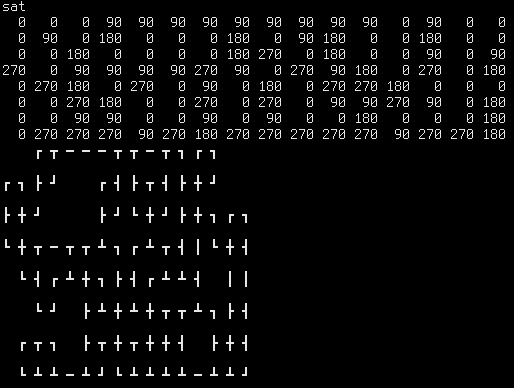
\includegraphics[scale=0.75]{\CURPATH/solver/solver.png}
\caption{Вывод скрипта солвера}
\end{figure}

Это работает $\approx 4$ секунды на моем старом и медленном Intel Atom N455 1.66GHz.
Быстро ли это? Не знаю, но снова вот что действительно круто, это то что мы понятия не имеем о какой-то математической
теории за всем этим, мы просто объявили ячейки, (полу-)стыки и определили отношения между ними.

Теперь следующий вопрос это, сколько здесь возможных решений?
Используя раннее описанный метод (\ref{SMTEnumerate}), я немного изменил скрипт солвера
\footnote{\url{.../solver/solve_pipe_puzzle2.py}} и солвер
сказал что возможно два решения.

Сравним их используя gvimdiff:

\begin{figure}[H]
\centering
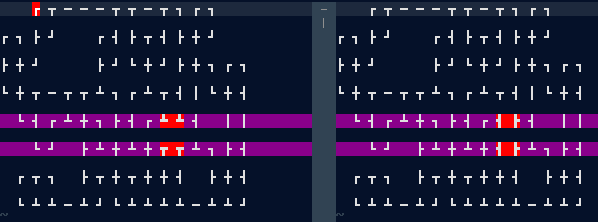
\includegraphics[scale=0.75]{\CURPATH/solver/diff.png}
\caption{Вывод gvimdiff (извините за мой красный курсор в левой части в левом верхнем углу)}
\end{figure}

4 ячейки в середине могут быть ориентированы по-разному.
Видимо, другие головоломки могут также выдавать разные результаты.

P.S.
\textit{Полу-стык} определен как булевый тип.
Но на самом деле, первая версия солвера была написана используя целочисленный тип для полу-стыков,
и 0 использовалось для False и 1 для True.
Я так сделал, потому что хотел более компактный исходный код, без использования длинных слов как ``False'' и ``True''.
И это работало, но медленнее. Вероятно, Z3 работает с булевыми типами быстрее? Лучше?
Так или иначе, я пишу это чтобы отметить, что, если нужно, целочисленный тип можно использовать вместо булевого.


\section{Развлекательная математика и головоломки}

\input{puzzles/sudoku/main_RU}
\input{puzzles/zebra/main_RU}
\input{puzzles/pipe/main_RU}
\input{puzzles/rubik2/failed_SMT/main_RU}
\input{puzzles/rubik2/SAT/main_RU}
\input{puzzles/rubik3/one_face_SMT/main_RU}
%\input{puzzles/numberlink/main_RU}
%\input{puzzles/two_parks_RU}
\input{puzzles/alphametics/main_RU}
%\input{puzzles/2015_AIME_II_Problems_12_RU}
%\input{puzzles/fred/main_RU}
%\input{puzzles/MC/main_RU}
%\input{puzzles/coin_flip/main_RU}
%\input{puzzles/Mock_AIME_2_2006-2007_Problem_8_RU}
%\input{puzzles/2012_AIME_I_Problems_1_RU}
%\input{puzzles/keypad_RU}


\section{Развлекательная математика и головоломки}

\input{puzzles/sudoku/main_RU}
\input{puzzles/zebra/main_RU}
\input{puzzles/pipe/main_RU}
\input{puzzles/rubik2/failed_SMT/main_RU}
\input{puzzles/rubik2/SAT/main_RU}
\input{puzzles/rubik3/one_face_SMT/main_RU}
%\input{puzzles/numberlink/main_RU}
%\input{puzzles/two_parks_RU}
\input{puzzles/alphametics/main_RU}
%\input{puzzles/2015_AIME_II_Problems_12_RU}
%\input{puzzles/fred/main_RU}
%\input{puzzles/MC/main_RU}
%\input{puzzles/coin_flip/main_RU}
%\input{puzzles/Mock_AIME_2_2006-2007_Problem_8_RU}
%\input{puzzles/2012_AIME_I_Problems_1_RU}
%\input{puzzles/keypad_RU}


\section{Развлекательная математика и головоломки}

\input{puzzles/sudoku/main_RU}
\input{puzzles/zebra/main_RU}
\input{puzzles/pipe/main_RU}
\input{puzzles/rubik2/failed_SMT/main_RU}
\input{puzzles/rubik2/SAT/main_RU}
\input{puzzles/rubik3/one_face_SMT/main_RU}
%\input{puzzles/numberlink/main_RU}
%\input{puzzles/two_parks_RU}
\input{puzzles/alphametics/main_RU}
%\input{puzzles/2015_AIME_II_Problems_12_RU}
%\input{puzzles/fred/main_RU}
%\input{puzzles/MC/main_RU}
%\input{puzzles/coin_flip/main_RU}
%\input{puzzles/Mock_AIME_2_2006-2007_Problem_8_RU}
%\input{puzzles/2012_AIME_I_Problems_1_RU}
%\input{puzzles/keypad_RU}


%\section{Развлекательная математика и головоломки}

\input{puzzles/sudoku/main_RU}
\input{puzzles/zebra/main_RU}
\input{puzzles/pipe/main_RU}
\input{puzzles/rubik2/failed_SMT/main_RU}
\input{puzzles/rubik2/SAT/main_RU}
\input{puzzles/rubik3/one_face_SMT/main_RU}
%\input{puzzles/numberlink/main_RU}
%\input{puzzles/two_parks_RU}
\input{puzzles/alphametics/main_RU}
%\input{puzzles/2015_AIME_II_Problems_12_RU}
%\input{puzzles/fred/main_RU}
%\input{puzzles/MC/main_RU}
%\input{puzzles/coin_flip/main_RU}
%\input{puzzles/Mock_AIME_2_2006-2007_Problem_8_RU}
%\input{puzzles/2012_AIME_I_Problems_1_RU}
%\input{puzzles/keypad_RU}


%\input{puzzles/two_parks_RU}
\subsection{Альфаметика}

Согласно Дональду Кнуту, термин ``Альфаметика'' был придуман Дж. Эйч. Аш. Хантером.
Это головоломка: какие десятичные цифры в пределах 0..9 нужно присвоить каждой букве, чтобы это уравнение было справедливо?

\begin{lstlisting}
  SEND
+ MORE
 -----
 MONEY
\end{lstlisting}

Для Z3 это легко:

\lstinputlisting{puzzles/alphametics/alpha.py}

Вывод:

\begin{lstlisting}
sat
[E, = 5,
 S, = 9,
 M, = 1,
 N, = 6,
 D, = 7,
 R, = 8,
 O, = 0,
 Y = 2]
\end{lstlisting}

Вот еще одна, из \ac{TAOCP} том IV (\url{http://www-cs-faculty.stanford.edu/~uno/fasc2b.ps.gz}):

\lstinputlisting{puzzles/alphametics/alpha2.py}

\begin{lstlisting}
sat
[L, = 6,
 S, = 7,
 N, = 2,
 T, = 1,
 I, = 5,
 V = 3,
 A, = 8,
 R, = 9,
 O, = 4,
 TRIO = 1954,
 SONATA, = 742818,
 VIOLA, = 35468,
 VIOLIN, = 354652]
\end{lstlisting}

% TODO URL
Эту головоломку я нашел в примерах pySMT:

\lstinputlisting{puzzles/alphametics/alpha3.py}

\begin{lstlisting}
sat
[D = 5, R = 4, O = 3, E = 8, L = 6, W = 7, H = 2]
\end{lstlisting}

%%% 

Это упражнение Q209 из
[Companion to the Papers of Donald Knuth]\footnote{\url{http://www-cs-faculty.stanford.edu/~knuth/cp.html}}.

\begin{lstlisting}
 KNIFE
  FORK
 SPOON
  SOUP
------
SUPPER
\end{lstlisting}

В целях упрощения, я добавил ф-цию (list\_to\_expr()):

\lstinputlisting{puzzles/alphametics/alpha4.py}

\begin{lstlisting}
sat
[K = 7,
 N = 4,
 R = 9,
 I = 1,
 E = 6,
 S = 0,
 O = 3,
 F = 5,
 U = 8,
 P = 2,
 SUPPER = 82269,
 SOUP = 382,
 SPOON = 2334,
 FORK = 5397,
 KNIFE = 74156]
\end{lstlisting}

S это 0, так что значение SUPPER начинается с (убранного) нуля. Скажем так, нам это не нравится.
Добавим это, чтобы это исправить:

\begin{lstlisting}
s.add(S!=0)
\end{lstlisting}

\begin{lstlisting}
sat
[K = 8,
 N = 4,
 R = 3,
 I = 7,
 E = 6,
 S = 1,
 O = 9,
 F = 2,
 U = 0,
 P = 5,
 SUPPER = 105563,
 SOUP = 1905,
 SPOON = 15994,
 FORK = 2938,
 KNIFE = 84726]
\end{lstlisting}

\paragraph{Создание своей собственной головоломки}

Вот проблема: есть только 10 букв, но как их выбрать из числа слов?
Мы можем использовать Z3 для этого:

\lstinputlisting{puzzles/alphametics/gen.py}

Это первая сгенерированная головоломка:

\begin{lstlisting}
sat
EGGS
JELLY
LUNCH
C 5
E 6
G 3
H 7
J 0
L 1
N 4
S 8
U 2
Y 9
\end{lstlisting}

Что если мы хотим, чтобы слово ``CAKE'' присутствовало в числе ``слагаемых''?

Добавим это:

\begin{lstlisting}
s.add(word_used[words.index('CAKE')])
\end{lstlisting}

\begin{lstlisting}
sat
CAKE
TEA
LUNCH
A 8
C 3
E 1
H 9
J 6
K 2
L 0
N 5
T 7
U 4
\end{lstlisting}

Добавим это:

\begin{lstlisting}
s.add(word_used[words.index('EGGS')])
\end{lstlisting}

Теперь оно может найти пару к EGGS:

\begin{lstlisting}
sat
EGGS
HONEY
LUNCH
C 6
E 7
G 9
H 4
L 5
N 8
O 2
S 3
U 0
Y 1
\end{lstlisting}

\paragraph{Файлы}

\url{https://github.com/DennisYurichev/...}




%\input{puzzles/2015_AIME_II_Problems_12_RU}
%\section{Развлекательная математика и головоломки}

\input{puzzles/sudoku/main_RU}
\input{puzzles/zebra/main_RU}
\input{puzzles/pipe/main_RU}
\input{puzzles/rubik2/failed_SMT/main_RU}
\input{puzzles/rubik2/SAT/main_RU}
\input{puzzles/rubik3/one_face_SMT/main_RU}
%\input{puzzles/numberlink/main_RU}
%\input{puzzles/two_parks_RU}
\input{puzzles/alphametics/main_RU}
%\input{puzzles/2015_AIME_II_Problems_12_RU}
%\input{puzzles/fred/main_RU}
%\input{puzzles/MC/main_RU}
%\input{puzzles/coin_flip/main_RU}
%\input{puzzles/Mock_AIME_2_2006-2007_Problem_8_RU}
%\input{puzzles/2012_AIME_I_Problems_1_RU}
%\input{puzzles/keypad_RU}


%\section{Развлекательная математика и головоломки}

\input{puzzles/sudoku/main_RU}
\input{puzzles/zebra/main_RU}
\input{puzzles/pipe/main_RU}
\input{puzzles/rubik2/failed_SMT/main_RU}
\input{puzzles/rubik2/SAT/main_RU}
\input{puzzles/rubik3/one_face_SMT/main_RU}
%\input{puzzles/numberlink/main_RU}
%\input{puzzles/two_parks_RU}
\input{puzzles/alphametics/main_RU}
%\input{puzzles/2015_AIME_II_Problems_12_RU}
%\input{puzzles/fred/main_RU}
%\input{puzzles/MC/main_RU}
%\input{puzzles/coin_flip/main_RU}
%\input{puzzles/Mock_AIME_2_2006-2007_Problem_8_RU}
%\input{puzzles/2012_AIME_I_Problems_1_RU}
%\input{puzzles/keypad_RU}


%\section{Развлекательная математика и головоломки}

\input{puzzles/sudoku/main_RU}
\input{puzzles/zebra/main_RU}
\input{puzzles/pipe/main_RU}
\input{puzzles/rubik2/failed_SMT/main_RU}
\input{puzzles/rubik2/SAT/main_RU}
\input{puzzles/rubik3/one_face_SMT/main_RU}
%\input{puzzles/numberlink/main_RU}
%\input{puzzles/two_parks_RU}
\input{puzzles/alphametics/main_RU}
%\input{puzzles/2015_AIME_II_Problems_12_RU}
%\input{puzzles/fred/main_RU}
%\input{puzzles/MC/main_RU}
%\input{puzzles/coin_flip/main_RU}
%\input{puzzles/Mock_AIME_2_2006-2007_Problem_8_RU}
%\input{puzzles/2012_AIME_I_Problems_1_RU}
%\input{puzzles/keypad_RU}


%\input{puzzles/Mock_AIME_2_2006-2007_Problem_8_RU}
%\input{puzzles/2012_AIME_I_Problems_1_RU}
%\input{puzzles/keypad_RU}


%\input{puzzles/two_parks_RU}
\subsection{Альфаметика}

Согласно Дональду Кнуту, термин ``Альфаметика'' был придуман Дж. Эйч. Аш. Хантером.
Это головоломка: какие десятичные цифры в пределах 0..9 нужно присвоить каждой букве, чтобы это уравнение было справедливо?

\begin{lstlisting}
  SEND
+ MORE
 -----
 MONEY
\end{lstlisting}

Для Z3 это легко:

\lstinputlisting{puzzles/alphametics/alpha.py}

Вывод:

\begin{lstlisting}
sat
[E, = 5,
 S, = 9,
 M, = 1,
 N, = 6,
 D, = 7,
 R, = 8,
 O, = 0,
 Y = 2]
\end{lstlisting}

Вот еще одна, из \ac{TAOCP} том IV (\url{http://www-cs-faculty.stanford.edu/~uno/fasc2b.ps.gz}):

\lstinputlisting{puzzles/alphametics/alpha2.py}

\begin{lstlisting}
sat
[L, = 6,
 S, = 7,
 N, = 2,
 T, = 1,
 I, = 5,
 V = 3,
 A, = 8,
 R, = 9,
 O, = 4,
 TRIO = 1954,
 SONATA, = 742818,
 VIOLA, = 35468,
 VIOLIN, = 354652]
\end{lstlisting}

% TODO URL
Эту головоломку я нашел в примерах pySMT:

\lstinputlisting{puzzles/alphametics/alpha3.py}

\begin{lstlisting}
sat
[D = 5, R = 4, O = 3, E = 8, L = 6, W = 7, H = 2]
\end{lstlisting}

%%% 

Это упражнение Q209 из
[Companion to the Papers of Donald Knuth]\footnote{\url{http://www-cs-faculty.stanford.edu/~knuth/cp.html}}.

\begin{lstlisting}
 KNIFE
  FORK
 SPOON
  SOUP
------
SUPPER
\end{lstlisting}

В целях упрощения, я добавил ф-цию (list\_to\_expr()):

\lstinputlisting{puzzles/alphametics/alpha4.py}

\begin{lstlisting}
sat
[K = 7,
 N = 4,
 R = 9,
 I = 1,
 E = 6,
 S = 0,
 O = 3,
 F = 5,
 U = 8,
 P = 2,
 SUPPER = 82269,
 SOUP = 382,
 SPOON = 2334,
 FORK = 5397,
 KNIFE = 74156]
\end{lstlisting}

S это 0, так что значение SUPPER начинается с (убранного) нуля. Скажем так, нам это не нравится.
Добавим это, чтобы это исправить:

\begin{lstlisting}
s.add(S!=0)
\end{lstlisting}

\begin{lstlisting}
sat
[K = 8,
 N = 4,
 R = 3,
 I = 7,
 E = 6,
 S = 1,
 O = 9,
 F = 2,
 U = 0,
 P = 5,
 SUPPER = 105563,
 SOUP = 1905,
 SPOON = 15994,
 FORK = 2938,
 KNIFE = 84726]
\end{lstlisting}

\paragraph{Создание своей собственной головоломки}

Вот проблема: есть только 10 букв, но как их выбрать из числа слов?
Мы можем использовать Z3 для этого:

\lstinputlisting{puzzles/alphametics/gen.py}

Это первая сгенерированная головоломка:

\begin{lstlisting}
sat
EGGS
JELLY
LUNCH
C 5
E 6
G 3
H 7
J 0
L 1
N 4
S 8
U 2
Y 9
\end{lstlisting}

Что если мы хотим, чтобы слово ``CAKE'' присутствовало в числе ``слагаемых''?

Добавим это:

\begin{lstlisting}
s.add(word_used[words.index('CAKE')])
\end{lstlisting}

\begin{lstlisting}
sat
CAKE
TEA
LUNCH
A 8
C 3
E 1
H 9
J 6
K 2
L 0
N 5
T 7
U 4
\end{lstlisting}

Добавим это:

\begin{lstlisting}
s.add(word_used[words.index('EGGS')])
\end{lstlisting}

Теперь оно может найти пару к EGGS:

\begin{lstlisting}
sat
EGGS
HONEY
LUNCH
C 6
E 7
G 9
H 4
L 5
N 8
O 2
S 3
U 0
Y 1
\end{lstlisting}

\paragraph{Файлы}

\url{https://github.com/DennisYurichev/...}




%\input{puzzles/2015_AIME_II_Problems_12_RU}
%\section{Развлекательная математика и головоломки}

\subsection{Судоку}

Головоломка Судоку это решетка 9*9, некоторые ячейки заполнены значениями, некоторые пустые:

% copypasted from http://www.texample.net/tikz/examples/sudoku/
\newcounter{row}
\newcounter{col}

\newcommand\setrow[9]{
  \setcounter{col}{1}
  \foreach \n in {#1, #2, #3, #4, #5, #6, #7, #8, #9} {
    \edef\x{\value{col} - 0.5}
    \edef\y{9.5 - \value{row}}
    \node[anchor=center] at (\x, \y) {\n};
    \stepcounter{col}
  }
  \stepcounter{row}
}

\begin{center}
\begin{tikzpicture}[scale=.7]
  \begin{scope}
    \draw (0, 0) grid (9, 9);
    \draw[very thick, scale=3] (0, 0) grid (3, 3);

    \setcounter{row}{1}
    \setrow { }{ }{5}  {3}{ }{ }  { }{ }{ }
    \setrow {8}{ }{ }  { }{ }{ }  { }{2}{ }
    \setrow { }{7}{ }  { }{1}{ }  {5}{ }{ }

    \setrow {4}{ }{ }  { }{ }{5}  {3}{ }{ }
    \setrow { }{1}{ }  { }{7}{ }  { }{ }{6}
    \setrow { }{ }{3}  {2}{ }{ }  { }{8}{ }

    \setrow { }{6}{ }  {5}{ }{ }  { }{ }{9}
    \setrow { }{ }{4}  { }{ }{ }  { }{3}{ }
    \setrow { }{ }{ }  { }{ }{9}  {7}{ }{ }

    \node[anchor=center] at (4.5, -0.5) {Нерешенная Судоку};
  \end{scope}
\end{tikzpicture}
\end{center}

Числа в каждом ряду должны быть уникальными, т.е., каждый ряд должен содержать 9 чисел в пределах 1..9 без повторений.
Та же история и для каждого столбца и каждого квадрата 3*3.

Головоломка представляет собой хороший кандидат, на котором можно попробовать \ac{SMT}-солвер, потому что это,
в общем-то, просто нерешенная система уравнений.

\input{puzzles/sudoku/1/main_RU}
%\input{puzzles/sudoku/GT/main_RU}
%\input{puzzles/sudoku/killer/main_RU}
\input{puzzles/sudoku/KLEE/main_RU}
\input{puzzles/sudoku/SAT/main_RU}


\subsection{Головоломка зебры (\ac{AKA} Загадка Эйнштейна)}

\input{puzzles/zebra/SMT/main_RU}
\input{puzzles/zebra/KLEE/main_RU}
\input{puzzles/zebra/SAT/main_RU}


\subsection{Решение головоломки ``трубы'' используя Z3 SMT-солвер}

\renewcommand{\CURPATH}{puzzles/pipe}

Головоломка ``трубы'' это популярная головоломка (просто погуглите ``pipe puzzle'' и посмотрите на картинки).

Вот как выглядит головоломка в разобранном виде:

\begin{figure}[H]
\label{fig:pipe_shuffled}
\centering
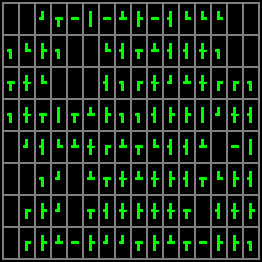
\includegraphics[scale=0.75]{\CURPATH/shuffled.png}
\caption{Разобранная головоломка}
\end{figure}

\dots и собранная:

\begin{figure}[H]
\label{fig:pipe_solved}
\centering
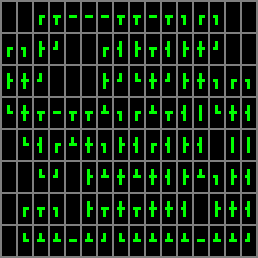
\includegraphics[scale=0.75]{\CURPATH/solved.png}
\caption{Собранная головоломка}
\end{figure}

Попробуем найти способ собрать её.

\subsubsection{Создание}

В начале, нужно её создать.
Вот простая идея.
Возьем массив ячеек 8*16.
Каждая ячейка может содержать какой-то тип блока.
Между ячейками есть стыки:

\input{\CURPATH/pipe_gen.tex}

Синие линии это горизонтальные стыки, красные линии это вертикальные стыки.
Мы просто случайно выставляем каждый стык в 0/false (отсутствует) или 1/true (присутствует).

После этого, теперь легко найти тип каждой ячейки.
А это:

\newcommand{\HeaderColor}{\cellcolor{blue!25}}
\begin{center}
\begin{longtable}{ | l | l | l | l | }
\hline
\HeaderColor стыки & \HeaderColor наше внутреннее название & \HeaderColor угол & \HeaderColor символ \\
\hline
0	&type 0		&	0$^{\circ}$	& (пробел)	\\
2	&type 2a	&	0$^{\circ}$	& \pmboxdrawuni{2503} \\ % ┃
2	&type 2a	&	90$^{\circ}$	& \pmboxdrawuni{2501} \\ % ━
2	&type 2b	&	0$^{\circ}$	& \pmboxdrawuni{250F} \\ % ┏
2	&type 2b	&	90$^{\circ}$	& \pmboxdrawuni{2513} \\ % ┓
2	&type 2b	&	180$^{\circ}$	& \pmboxdrawuni{251B} \\ % ┛
2	&type 2b	&	270$^{\circ}$	& \pmboxdrawuni{2517} \\ % ┗
3	&type 3		&	0$^{\circ}$	& \pmboxdrawuni{2523} \\ % ┣
3 	&type 3		&	90$^{\circ}$	& \pmboxdrawuni{2533} \\ % ┳
3	&type 3		&	180$^{\circ}$	& \pmboxdrawuni{252B} \\ % ┫
3	&type 3		&	270$^{\circ}$	& \pmboxdrawuni{253B} \\ % ┻
4	&type 4		&	0$^{\circ}$	& \pmboxdrawuni{254B} \\ % ╋
\hline
\end{longtable}
\end{center}

\textit{Висящие} стыки могут присутствовать на первой стадии (т.е., ячейки только с одним стыком), но они удалются
рекурсивно, и эти ячейки преобразуются в пустые ячейки.
Так что, в самом конце, все ячейки имеют минимум 2 стыка, и вся эта сантехническая система не имеет связей с внешним миром ---
я надеюсь, из-за этого станет немного проще.

Исходник генератора на Си здесь: \url{.../pipe/generator}.
Все вертикальные стыки хранятся в глобальном массиве \textit{hjoints[]} и вертикальные в \textit{vjoints[]}.

Программа на Си генерирует ANSI-раскрашенный вывод, как это было показано выше
(\ref{fig:pipe_shuffled}, \ref{fig:pipe_solved}) плюс массив типов для каждой ячейки, но без информации об углах:

\begin{lstlisting}[label=init_cells]
[
["0", "0", "2b", "3", "2a", "2a", "2a", "3", "3", "2a", "3", "2b", "2b", "2b", "0", "0"],
["2b", "2b", "3", "2b", "0", "0", "2b", "3", "3", "3", "3", "3", "4", "2b", "0", "0"],
["3", "4", "2b", "0", "0", "0", "3", "2b", "2b", "4", "2b", "3", "4", "2b", "2b", "2b"],
["2b", "4", "3", "2a", "3", "3", "3", "2b", "2b", "3", "3", "3", "2a", "2b", "4", "3"],
["0", "2b", "3", "2b", "3", "4", "2b", "3", "3", "2b", "3", "3", "3", "0", "2a", "2a"],
["0", "0", "2b", "2b", "0", "3", "3", "4", "3", "4", "3", "3", "3", "2b", "3", "3"],
["0", "2b", "3", "2b", "0", "3", "3", "4", "3", "4", "4", "3", "0", "3", "4", "3"],
["0", "2b", "3", "3", "2a", "3", "2b", "2b", "3", "3", "3", "3", "2a", "3", "3", "2b"],
]
\end{lstlisting}

\subsubsection{Решение}

Прежде всего, мы будем работать с массивом ячеек 8*16, где каждый элемент имеет 4 бита:
``T'' (top/верх),
``B'' (bottom/низ),
``L'' (left/лево),
``R'' (right/право).
Каждый бит представляет собой половину стыка.

\input{\CURPATH/pipe_solve.tex}

Теперь определяем массив для каждого из четырех полустыков + информация об угле:

\begin{lstlisting}
HEIGHT=8
WIDTH=16

# if T/B/R/L is Bool instead of Int, Z3 solver will work faster
T=[[Bool('cell_%d_%d_top' % (r, c)) for c in range(WIDTH)] for r in range(HEIGHT)]
B=[[Bool('cell_%d_%d_bottom' % (r, c)) for c in range(WIDTH)] for r in range(HEIGHT)]
R=[[Bool('cell_%d_%d_right' % (r, c)) for c in range(WIDTH)] for r in range(HEIGHT)]
L=[[Bool('cell_%d_%d_left' % (r, c)) for c in range(WIDTH)] for r in range(HEIGHT)]
A=[[Int('cell_%d_%d_angle' % (r, c)) for c in range(WIDTH)] for r in range(HEIGHT)]
\end{lstlisting}

Мы знаем, что если каждый из полустыков присутствует, ответный полустык также должен присутствовать, и наоборот. 
Определяем всё это используя эти констрайнты:

\begin{lstlisting}
# shorthand variables for True and False:
t=True
f=False

# "top" of each cell must be equal to "bottom" of the cell above
# "bottom" of each cell must be equal to "top" of the cell below
# "left" of each cell must be equal to "right" of the cell at left
# "right" of each cell must be equal to "left" of the cell at right
for r in range(HEIGHT):
    for c in range(WIDTH):
        if r!=0:
            s.add(T[r][c]==B[r-1][c])
        if r!=HEIGHT-1:
            s.add(B[r][c]==T[r+1][c])
        if c!=0:
            s.add(L[r][c]==R[r][c-1])
        if c!=WIDTH-1:
            s.add(R[r][c]==L[r][c+1])

# "left" of each cell of first column shouldn't have any connection
# so is "right" of each cell of the last column
for r in range(HEIGHT):
    s.add(L[r][0]==f)
    s.add(R[r][WIDTH-1]==f)

# "top" of each cell of the first row shouldn't have any connection
# so is "bottom" of each cell of the last row
for c in range(WIDTH):
    s.add(T[0][c]==f)
    s.add(B[HEIGHT-1][c]==f)
\end{lstlisting}

Теперь перебираем все ячейки в изначальном массиве (\ref{init_cells}).
Первые две ячейки здесь пустые. И третья имеет тип ``2b''.
Это ``\pmboxdrawuni{250F}'' % ┏
и его можно ориентировать четырьмя разными способами.
И если её угол это 0$^{\circ}$, верхний и правый полустыки присутствуют, остальные отсутствуют.
Если он имеет угол 90$^{\circ}$, он выглядит как 
``\pmboxdrawuni{2513}'', % ┓
и верхник и левый полустыки присутствуют, остальные отсутствуют.

На обычном русском языке: ``если ячейка этого типа имеет угол 0$^{\circ}$, вот эти полустыки должны присутствовать \textbf{ИЛИ}
если она имеет угол 90$^{\circ}$, эти полустыки должны присутствовать, \textbf{ИЛИ}, итд, итд.''

Точно также, мы определяем эти правила для всех типов и всех возможных углов:

\begin{lstlisting}
for r in range(HEIGHT):
    for c in range(WIDTH):
        ty=cells_type[r][c]

        if ty=="0":
            s.add(A[r][c]==f)
            s.add(T[r][c]==f, B[r][c]==f, L[r][c]==f, R[r][c]==f)

        if ty=="2a":
            s.add(Or(And(A[r][c]==0, L[r][c]==f, R[r][c]==f, T[r][c]==t, B[r][c]==t),   # §\pmboxdrawuni{2503}§
                    And(A[r][c]==90, L[r][c]==t, R[r][c]==t, T[r][c]==f, B[r][c]==f)))  # §\pmboxdrawuni{2501}§

        if ty=="2b":
            s.add(Or(And(A[r][c]==0, L[r][c]==f, R[r][c]==t, T[r][c]==f, B[r][c]==t),   # §\pmboxdrawuni{250F}§
                    And(A[r][c]==90, L[r][c]==t, R[r][c]==f, T[r][c]==f, B[r][c]==t),   # §\pmboxdrawuni{2513}§
                    And(A[r][c]==180, L[r][c]==t, R[r][c]==f, T[r][c]==t, B[r][c]==f),  # §\pmboxdrawuni{251B}§
                    And(A[r][c]==270, L[r][c]==f, R[r][c]==t, T[r][c]==t, B[r][c]==f))) # §\pmboxdrawuni{2517}§
	
        if ty=="3":
            s.add(Or(And(A[r][c]==0, L[r][c]==f, R[r][c]==t, T[r][c]==t, B[r][c]==t),   # §\pmboxdrawuni{2523}§
                    And(A[r][c]==90, L[r][c]==t, R[r][c]==t, T[r][c]==f, B[r][c]==t),   # §\pmboxdrawuni{2533}§
                    And(A[r][c]==180, L[r][c]==t, R[r][c]==f, T[r][c]==t, B[r][c]==t),  # §\pmboxdrawuni{252B}§
                    And(A[r][c]==270, L[r][c]==t, R[r][c]==t, T[r][c]==t, B[r][c]==f))) # §\pmboxdrawuni{253B}§

        if ty=="4":
            s.add(A[r][c]==0)
            s.add(T[r][c]==t, B[r][c]==t, L[r][c]==t, R[r][c]==t) # §\pmboxdrawuni{254B}§
\end{lstlisting}

Полный исходник здесь: \url{.../solver/solve_pipe_puzzle1.py}.

Получается такой результат (выводит угол для каждой ячейки и (псевдо)графическое представление):

\begin{figure}[H]
\centering
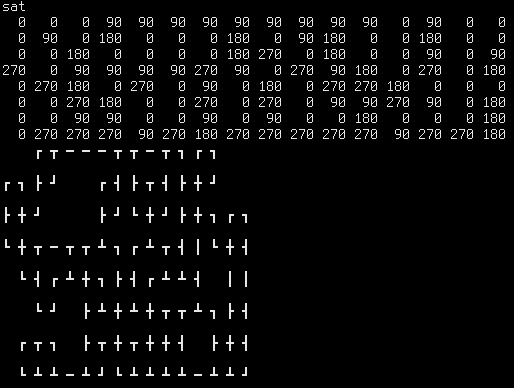
\includegraphics[scale=0.75]{\CURPATH/solver/solver.png}
\caption{Вывод скрипта солвера}
\end{figure}

Это работает $\approx 4$ секунды на моем старом и медленном Intel Atom N455 1.66GHz.
Быстро ли это? Не знаю, но снова вот что действительно круто, это то что мы понятия не имеем о какой-то математической
теории за всем этим, мы просто объявили ячейки, (полу-)стыки и определили отношения между ними.

Теперь следующий вопрос это, сколько здесь возможных решений?
Используя раннее описанный метод (\ref{SMTEnumerate}), я немного изменил скрипт солвера
\footnote{\url{.../solver/solve_pipe_puzzle2.py}} и солвер
сказал что возможно два решения.

Сравним их используя gvimdiff:

\begin{figure}[H]
\centering
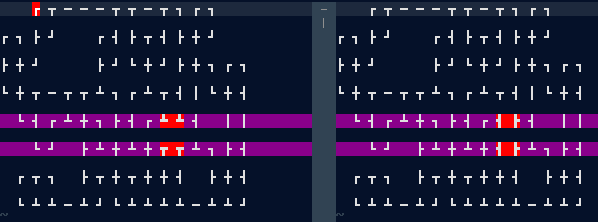
\includegraphics[scale=0.75]{\CURPATH/solver/diff.png}
\caption{Вывод gvimdiff (извините за мой красный курсор в левой части в левом верхнем углу)}
\end{figure}

4 ячейки в середине могут быть ориентированы по-разному.
Видимо, другие головоломки могут также выдавать разные результаты.

P.S.
\textit{Полу-стык} определен как булевый тип.
Но на самом деле, первая версия солвера была написана используя целочисленный тип для полу-стыков,
и 0 использовалось для False и 1 для True.
Я так сделал, потому что хотел более компактный исходный код, без использования длинных слов как ``False'' и ``True''.
И это работало, но медленнее. Вероятно, Z3 работает с булевыми типами быстрее? Лучше?
Так или иначе, я пишу это чтобы отметить, что, если нужно, целочисленный тип можно использовать вместо булевого.


\section{Развлекательная математика и головоломки}

\input{puzzles/sudoku/main_RU}
\input{puzzles/zebra/main_RU}
\input{puzzles/pipe/main_RU}
\input{puzzles/rubik2/failed_SMT/main_RU}
\input{puzzles/rubik2/SAT/main_RU}
\input{puzzles/rubik3/one_face_SMT/main_RU}
%\input{puzzles/numberlink/main_RU}
%\input{puzzles/two_parks_RU}
\input{puzzles/alphametics/main_RU}
%\input{puzzles/2015_AIME_II_Problems_12_RU}
%\input{puzzles/fred/main_RU}
%\input{puzzles/MC/main_RU}
%\input{puzzles/coin_flip/main_RU}
%\input{puzzles/Mock_AIME_2_2006-2007_Problem_8_RU}
%\input{puzzles/2012_AIME_I_Problems_1_RU}
%\input{puzzles/keypad_RU}


\section{Развлекательная математика и головоломки}

\input{puzzles/sudoku/main_RU}
\input{puzzles/zebra/main_RU}
\input{puzzles/pipe/main_RU}
\input{puzzles/rubik2/failed_SMT/main_RU}
\input{puzzles/rubik2/SAT/main_RU}
\input{puzzles/rubik3/one_face_SMT/main_RU}
%\input{puzzles/numberlink/main_RU}
%\input{puzzles/two_parks_RU}
\input{puzzles/alphametics/main_RU}
%\input{puzzles/2015_AIME_II_Problems_12_RU}
%\input{puzzles/fred/main_RU}
%\input{puzzles/MC/main_RU}
%\input{puzzles/coin_flip/main_RU}
%\input{puzzles/Mock_AIME_2_2006-2007_Problem_8_RU}
%\input{puzzles/2012_AIME_I_Problems_1_RU}
%\input{puzzles/keypad_RU}


\section{Развлекательная математика и головоломки}

\input{puzzles/sudoku/main_RU}
\input{puzzles/zebra/main_RU}
\input{puzzles/pipe/main_RU}
\input{puzzles/rubik2/failed_SMT/main_RU}
\input{puzzles/rubik2/SAT/main_RU}
\input{puzzles/rubik3/one_face_SMT/main_RU}
%\input{puzzles/numberlink/main_RU}
%\input{puzzles/two_parks_RU}
\input{puzzles/alphametics/main_RU}
%\input{puzzles/2015_AIME_II_Problems_12_RU}
%\input{puzzles/fred/main_RU}
%\input{puzzles/MC/main_RU}
%\input{puzzles/coin_flip/main_RU}
%\input{puzzles/Mock_AIME_2_2006-2007_Problem_8_RU}
%\input{puzzles/2012_AIME_I_Problems_1_RU}
%\input{puzzles/keypad_RU}


%\section{Развлекательная математика и головоломки}

\input{puzzles/sudoku/main_RU}
\input{puzzles/zebra/main_RU}
\input{puzzles/pipe/main_RU}
\input{puzzles/rubik2/failed_SMT/main_RU}
\input{puzzles/rubik2/SAT/main_RU}
\input{puzzles/rubik3/one_face_SMT/main_RU}
%\input{puzzles/numberlink/main_RU}
%\input{puzzles/two_parks_RU}
\input{puzzles/alphametics/main_RU}
%\input{puzzles/2015_AIME_II_Problems_12_RU}
%\input{puzzles/fred/main_RU}
%\input{puzzles/MC/main_RU}
%\input{puzzles/coin_flip/main_RU}
%\input{puzzles/Mock_AIME_2_2006-2007_Problem_8_RU}
%\input{puzzles/2012_AIME_I_Problems_1_RU}
%\input{puzzles/keypad_RU}


%\input{puzzles/two_parks_RU}
\subsection{Альфаметика}

Согласно Дональду Кнуту, термин ``Альфаметика'' был придуман Дж. Эйч. Аш. Хантером.
Это головоломка: какие десятичные цифры в пределах 0..9 нужно присвоить каждой букве, чтобы это уравнение было справедливо?

\begin{lstlisting}
  SEND
+ MORE
 -----
 MONEY
\end{lstlisting}

Для Z3 это легко:

\lstinputlisting{puzzles/alphametics/alpha.py}

Вывод:

\begin{lstlisting}
sat
[E, = 5,
 S, = 9,
 M, = 1,
 N, = 6,
 D, = 7,
 R, = 8,
 O, = 0,
 Y = 2]
\end{lstlisting}

Вот еще одна, из \ac{TAOCP} том IV (\url{http://www-cs-faculty.stanford.edu/~uno/fasc2b.ps.gz}):

\lstinputlisting{puzzles/alphametics/alpha2.py}

\begin{lstlisting}
sat
[L, = 6,
 S, = 7,
 N, = 2,
 T, = 1,
 I, = 5,
 V = 3,
 A, = 8,
 R, = 9,
 O, = 4,
 TRIO = 1954,
 SONATA, = 742818,
 VIOLA, = 35468,
 VIOLIN, = 354652]
\end{lstlisting}

% TODO URL
Эту головоломку я нашел в примерах pySMT:

\lstinputlisting{puzzles/alphametics/alpha3.py}

\begin{lstlisting}
sat
[D = 5, R = 4, O = 3, E = 8, L = 6, W = 7, H = 2]
\end{lstlisting}

%%% 

Это упражнение Q209 из
[Companion to the Papers of Donald Knuth]\footnote{\url{http://www-cs-faculty.stanford.edu/~knuth/cp.html}}.

\begin{lstlisting}
 KNIFE
  FORK
 SPOON
  SOUP
------
SUPPER
\end{lstlisting}

В целях упрощения, я добавил ф-цию (list\_to\_expr()):

\lstinputlisting{puzzles/alphametics/alpha4.py}

\begin{lstlisting}
sat
[K = 7,
 N = 4,
 R = 9,
 I = 1,
 E = 6,
 S = 0,
 O = 3,
 F = 5,
 U = 8,
 P = 2,
 SUPPER = 82269,
 SOUP = 382,
 SPOON = 2334,
 FORK = 5397,
 KNIFE = 74156]
\end{lstlisting}

S это 0, так что значение SUPPER начинается с (убранного) нуля. Скажем так, нам это не нравится.
Добавим это, чтобы это исправить:

\begin{lstlisting}
s.add(S!=0)
\end{lstlisting}

\begin{lstlisting}
sat
[K = 8,
 N = 4,
 R = 3,
 I = 7,
 E = 6,
 S = 1,
 O = 9,
 F = 2,
 U = 0,
 P = 5,
 SUPPER = 105563,
 SOUP = 1905,
 SPOON = 15994,
 FORK = 2938,
 KNIFE = 84726]
\end{lstlisting}

\paragraph{Создание своей собственной головоломки}

Вот проблема: есть только 10 букв, но как их выбрать из числа слов?
Мы можем использовать Z3 для этого:

\lstinputlisting{puzzles/alphametics/gen.py}

Это первая сгенерированная головоломка:

\begin{lstlisting}
sat
EGGS
JELLY
LUNCH
C 5
E 6
G 3
H 7
J 0
L 1
N 4
S 8
U 2
Y 9
\end{lstlisting}

Что если мы хотим, чтобы слово ``CAKE'' присутствовало в числе ``слагаемых''?

Добавим это:

\begin{lstlisting}
s.add(word_used[words.index('CAKE')])
\end{lstlisting}

\begin{lstlisting}
sat
CAKE
TEA
LUNCH
A 8
C 3
E 1
H 9
J 6
K 2
L 0
N 5
T 7
U 4
\end{lstlisting}

Добавим это:

\begin{lstlisting}
s.add(word_used[words.index('EGGS')])
\end{lstlisting}

Теперь оно может найти пару к EGGS:

\begin{lstlisting}
sat
EGGS
HONEY
LUNCH
C 6
E 7
G 9
H 4
L 5
N 8
O 2
S 3
U 0
Y 1
\end{lstlisting}

\paragraph{Файлы}

\url{https://github.com/DennisYurichev/...}




%\input{puzzles/2015_AIME_II_Problems_12_RU}
%\section{Развлекательная математика и головоломки}

\input{puzzles/sudoku/main_RU}
\input{puzzles/zebra/main_RU}
\input{puzzles/pipe/main_RU}
\input{puzzles/rubik2/failed_SMT/main_RU}
\input{puzzles/rubik2/SAT/main_RU}
\input{puzzles/rubik3/one_face_SMT/main_RU}
%\input{puzzles/numberlink/main_RU}
%\input{puzzles/two_parks_RU}
\input{puzzles/alphametics/main_RU}
%\input{puzzles/2015_AIME_II_Problems_12_RU}
%\input{puzzles/fred/main_RU}
%\input{puzzles/MC/main_RU}
%\input{puzzles/coin_flip/main_RU}
%\input{puzzles/Mock_AIME_2_2006-2007_Problem_8_RU}
%\input{puzzles/2012_AIME_I_Problems_1_RU}
%\input{puzzles/keypad_RU}


%\section{Развлекательная математика и головоломки}

\input{puzzles/sudoku/main_RU}
\input{puzzles/zebra/main_RU}
\input{puzzles/pipe/main_RU}
\input{puzzles/rubik2/failed_SMT/main_RU}
\input{puzzles/rubik2/SAT/main_RU}
\input{puzzles/rubik3/one_face_SMT/main_RU}
%\input{puzzles/numberlink/main_RU}
%\input{puzzles/two_parks_RU}
\input{puzzles/alphametics/main_RU}
%\input{puzzles/2015_AIME_II_Problems_12_RU}
%\input{puzzles/fred/main_RU}
%\input{puzzles/MC/main_RU}
%\input{puzzles/coin_flip/main_RU}
%\input{puzzles/Mock_AIME_2_2006-2007_Problem_8_RU}
%\input{puzzles/2012_AIME_I_Problems_1_RU}
%\input{puzzles/keypad_RU}


%\section{Развлекательная математика и головоломки}

\input{puzzles/sudoku/main_RU}
\input{puzzles/zebra/main_RU}
\input{puzzles/pipe/main_RU}
\input{puzzles/rubik2/failed_SMT/main_RU}
\input{puzzles/rubik2/SAT/main_RU}
\input{puzzles/rubik3/one_face_SMT/main_RU}
%\input{puzzles/numberlink/main_RU}
%\input{puzzles/two_parks_RU}
\input{puzzles/alphametics/main_RU}
%\input{puzzles/2015_AIME_II_Problems_12_RU}
%\input{puzzles/fred/main_RU}
%\input{puzzles/MC/main_RU}
%\input{puzzles/coin_flip/main_RU}
%\input{puzzles/Mock_AIME_2_2006-2007_Problem_8_RU}
%\input{puzzles/2012_AIME_I_Problems_1_RU}
%\input{puzzles/keypad_RU}


%\input{puzzles/Mock_AIME_2_2006-2007_Problem_8_RU}
%\input{puzzles/2012_AIME_I_Problems_1_RU}
%\input{puzzles/keypad_RU}


%\section{Развлекательная математика и головоломки}

\subsection{Судоку}

Головоломка Судоку это решетка 9*9, некоторые ячейки заполнены значениями, некоторые пустые:

% copypasted from http://www.texample.net/tikz/examples/sudoku/
\newcounter{row}
\newcounter{col}

\newcommand\setrow[9]{
  \setcounter{col}{1}
  \foreach \n in {#1, #2, #3, #4, #5, #6, #7, #8, #9} {
    \edef\x{\value{col} - 0.5}
    \edef\y{9.5 - \value{row}}
    \node[anchor=center] at (\x, \y) {\n};
    \stepcounter{col}
  }
  \stepcounter{row}
}

\begin{center}
\begin{tikzpicture}[scale=.7]
  \begin{scope}
    \draw (0, 0) grid (9, 9);
    \draw[very thick, scale=3] (0, 0) grid (3, 3);

    \setcounter{row}{1}
    \setrow { }{ }{5}  {3}{ }{ }  { }{ }{ }
    \setrow {8}{ }{ }  { }{ }{ }  { }{2}{ }
    \setrow { }{7}{ }  { }{1}{ }  {5}{ }{ }

    \setrow {4}{ }{ }  { }{ }{5}  {3}{ }{ }
    \setrow { }{1}{ }  { }{7}{ }  { }{ }{6}
    \setrow { }{ }{3}  {2}{ }{ }  { }{8}{ }

    \setrow { }{6}{ }  {5}{ }{ }  { }{ }{9}
    \setrow { }{ }{4}  { }{ }{ }  { }{3}{ }
    \setrow { }{ }{ }  { }{ }{9}  {7}{ }{ }

    \node[anchor=center] at (4.5, -0.5) {Нерешенная Судоку};
  \end{scope}
\end{tikzpicture}
\end{center}

Числа в каждом ряду должны быть уникальными, т.е., каждый ряд должен содержать 9 чисел в пределах 1..9 без повторений.
Та же история и для каждого столбца и каждого квадрата 3*3.

Головоломка представляет собой хороший кандидат, на котором можно попробовать \ac{SMT}-солвер, потому что это,
в общем-то, просто нерешенная система уравнений.

\input{puzzles/sudoku/1/main_RU}
%\input{puzzles/sudoku/GT/main_RU}
%\input{puzzles/sudoku/killer/main_RU}
\input{puzzles/sudoku/KLEE/main_RU}
\input{puzzles/sudoku/SAT/main_RU}


\subsection{Головоломка зебры (\ac{AKA} Загадка Эйнштейна)}

\input{puzzles/zebra/SMT/main_RU}
\input{puzzles/zebra/KLEE/main_RU}
\input{puzzles/zebra/SAT/main_RU}


\subsection{Решение головоломки ``трубы'' используя Z3 SMT-солвер}

\renewcommand{\CURPATH}{puzzles/pipe}

Головоломка ``трубы'' это популярная головоломка (просто погуглите ``pipe puzzle'' и посмотрите на картинки).

Вот как выглядит головоломка в разобранном виде:

\begin{figure}[H]
\label{fig:pipe_shuffled}
\centering
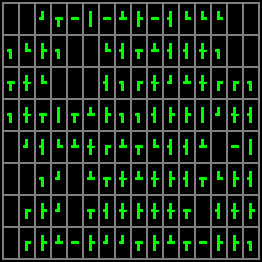
\includegraphics[scale=0.75]{\CURPATH/shuffled.png}
\caption{Разобранная головоломка}
\end{figure}

\dots и собранная:

\begin{figure}[H]
\label{fig:pipe_solved}
\centering
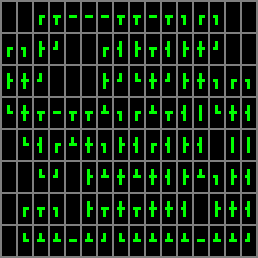
\includegraphics[scale=0.75]{\CURPATH/solved.png}
\caption{Собранная головоломка}
\end{figure}

Попробуем найти способ собрать её.

\subsubsection{Создание}

В начале, нужно её создать.
Вот простая идея.
Возьем массив ячеек 8*16.
Каждая ячейка может содержать какой-то тип блока.
Между ячейками есть стыки:

\input{\CURPATH/pipe_gen.tex}

Синие линии это горизонтальные стыки, красные линии это вертикальные стыки.
Мы просто случайно выставляем каждый стык в 0/false (отсутствует) или 1/true (присутствует).

После этого, теперь легко найти тип каждой ячейки.
А это:

\newcommand{\HeaderColor}{\cellcolor{blue!25}}
\begin{center}
\begin{longtable}{ | l | l | l | l | }
\hline
\HeaderColor стыки & \HeaderColor наше внутреннее название & \HeaderColor угол & \HeaderColor символ \\
\hline
0	&type 0		&	0$^{\circ}$	& (пробел)	\\
2	&type 2a	&	0$^{\circ}$	& \pmboxdrawuni{2503} \\ % ┃
2	&type 2a	&	90$^{\circ}$	& \pmboxdrawuni{2501} \\ % ━
2	&type 2b	&	0$^{\circ}$	& \pmboxdrawuni{250F} \\ % ┏
2	&type 2b	&	90$^{\circ}$	& \pmboxdrawuni{2513} \\ % ┓
2	&type 2b	&	180$^{\circ}$	& \pmboxdrawuni{251B} \\ % ┛
2	&type 2b	&	270$^{\circ}$	& \pmboxdrawuni{2517} \\ % ┗
3	&type 3		&	0$^{\circ}$	& \pmboxdrawuni{2523} \\ % ┣
3 	&type 3		&	90$^{\circ}$	& \pmboxdrawuni{2533} \\ % ┳
3	&type 3		&	180$^{\circ}$	& \pmboxdrawuni{252B} \\ % ┫
3	&type 3		&	270$^{\circ}$	& \pmboxdrawuni{253B} \\ % ┻
4	&type 4		&	0$^{\circ}$	& \pmboxdrawuni{254B} \\ % ╋
\hline
\end{longtable}
\end{center}

\textit{Висящие} стыки могут присутствовать на первой стадии (т.е., ячейки только с одним стыком), но они удалются
рекурсивно, и эти ячейки преобразуются в пустые ячейки.
Так что, в самом конце, все ячейки имеют минимум 2 стыка, и вся эта сантехническая система не имеет связей с внешним миром ---
я надеюсь, из-за этого станет немного проще.

Исходник генератора на Си здесь: \url{.../pipe/generator}.
Все вертикальные стыки хранятся в глобальном массиве \textit{hjoints[]} и вертикальные в \textit{vjoints[]}.

Программа на Си генерирует ANSI-раскрашенный вывод, как это было показано выше
(\ref{fig:pipe_shuffled}, \ref{fig:pipe_solved}) плюс массив типов для каждой ячейки, но без информации об углах:

\begin{lstlisting}[label=init_cells]
[
["0", "0", "2b", "3", "2a", "2a", "2a", "3", "3", "2a", "3", "2b", "2b", "2b", "0", "0"],
["2b", "2b", "3", "2b", "0", "0", "2b", "3", "3", "3", "3", "3", "4", "2b", "0", "0"],
["3", "4", "2b", "0", "0", "0", "3", "2b", "2b", "4", "2b", "3", "4", "2b", "2b", "2b"],
["2b", "4", "3", "2a", "3", "3", "3", "2b", "2b", "3", "3", "3", "2a", "2b", "4", "3"],
["0", "2b", "3", "2b", "3", "4", "2b", "3", "3", "2b", "3", "3", "3", "0", "2a", "2a"],
["0", "0", "2b", "2b", "0", "3", "3", "4", "3", "4", "3", "3", "3", "2b", "3", "3"],
["0", "2b", "3", "2b", "0", "3", "3", "4", "3", "4", "4", "3", "0", "3", "4", "3"],
["0", "2b", "3", "3", "2a", "3", "2b", "2b", "3", "3", "3", "3", "2a", "3", "3", "2b"],
]
\end{lstlisting}

\subsubsection{Решение}

Прежде всего, мы будем работать с массивом ячеек 8*16, где каждый элемент имеет 4 бита:
``T'' (top/верх),
``B'' (bottom/низ),
``L'' (left/лево),
``R'' (right/право).
Каждый бит представляет собой половину стыка.

\input{\CURPATH/pipe_solve.tex}

Теперь определяем массив для каждого из четырех полустыков + информация об угле:

\begin{lstlisting}
HEIGHT=8
WIDTH=16

# if T/B/R/L is Bool instead of Int, Z3 solver will work faster
T=[[Bool('cell_%d_%d_top' % (r, c)) for c in range(WIDTH)] for r in range(HEIGHT)]
B=[[Bool('cell_%d_%d_bottom' % (r, c)) for c in range(WIDTH)] for r in range(HEIGHT)]
R=[[Bool('cell_%d_%d_right' % (r, c)) for c in range(WIDTH)] for r in range(HEIGHT)]
L=[[Bool('cell_%d_%d_left' % (r, c)) for c in range(WIDTH)] for r in range(HEIGHT)]
A=[[Int('cell_%d_%d_angle' % (r, c)) for c in range(WIDTH)] for r in range(HEIGHT)]
\end{lstlisting}

Мы знаем, что если каждый из полустыков присутствует, ответный полустык также должен присутствовать, и наоборот. 
Определяем всё это используя эти констрайнты:

\begin{lstlisting}
# shorthand variables for True and False:
t=True
f=False

# "top" of each cell must be equal to "bottom" of the cell above
# "bottom" of each cell must be equal to "top" of the cell below
# "left" of each cell must be equal to "right" of the cell at left
# "right" of each cell must be equal to "left" of the cell at right
for r in range(HEIGHT):
    for c in range(WIDTH):
        if r!=0:
            s.add(T[r][c]==B[r-1][c])
        if r!=HEIGHT-1:
            s.add(B[r][c]==T[r+1][c])
        if c!=0:
            s.add(L[r][c]==R[r][c-1])
        if c!=WIDTH-1:
            s.add(R[r][c]==L[r][c+1])

# "left" of each cell of first column shouldn't have any connection
# so is "right" of each cell of the last column
for r in range(HEIGHT):
    s.add(L[r][0]==f)
    s.add(R[r][WIDTH-1]==f)

# "top" of each cell of the first row shouldn't have any connection
# so is "bottom" of each cell of the last row
for c in range(WIDTH):
    s.add(T[0][c]==f)
    s.add(B[HEIGHT-1][c]==f)
\end{lstlisting}

Теперь перебираем все ячейки в изначальном массиве (\ref{init_cells}).
Первые две ячейки здесь пустые. И третья имеет тип ``2b''.
Это ``\pmboxdrawuni{250F}'' % ┏
и его можно ориентировать четырьмя разными способами.
И если её угол это 0$^{\circ}$, верхний и правый полустыки присутствуют, остальные отсутствуют.
Если он имеет угол 90$^{\circ}$, он выглядит как 
``\pmboxdrawuni{2513}'', % ┓
и верхник и левый полустыки присутствуют, остальные отсутствуют.

На обычном русском языке: ``если ячейка этого типа имеет угол 0$^{\circ}$, вот эти полустыки должны присутствовать \textbf{ИЛИ}
если она имеет угол 90$^{\circ}$, эти полустыки должны присутствовать, \textbf{ИЛИ}, итд, итд.''

Точно также, мы определяем эти правила для всех типов и всех возможных углов:

\begin{lstlisting}
for r in range(HEIGHT):
    for c in range(WIDTH):
        ty=cells_type[r][c]

        if ty=="0":
            s.add(A[r][c]==f)
            s.add(T[r][c]==f, B[r][c]==f, L[r][c]==f, R[r][c]==f)

        if ty=="2a":
            s.add(Or(And(A[r][c]==0, L[r][c]==f, R[r][c]==f, T[r][c]==t, B[r][c]==t),   # §\pmboxdrawuni{2503}§
                    And(A[r][c]==90, L[r][c]==t, R[r][c]==t, T[r][c]==f, B[r][c]==f)))  # §\pmboxdrawuni{2501}§

        if ty=="2b":
            s.add(Or(And(A[r][c]==0, L[r][c]==f, R[r][c]==t, T[r][c]==f, B[r][c]==t),   # §\pmboxdrawuni{250F}§
                    And(A[r][c]==90, L[r][c]==t, R[r][c]==f, T[r][c]==f, B[r][c]==t),   # §\pmboxdrawuni{2513}§
                    And(A[r][c]==180, L[r][c]==t, R[r][c]==f, T[r][c]==t, B[r][c]==f),  # §\pmboxdrawuni{251B}§
                    And(A[r][c]==270, L[r][c]==f, R[r][c]==t, T[r][c]==t, B[r][c]==f))) # §\pmboxdrawuni{2517}§
	
        if ty=="3":
            s.add(Or(And(A[r][c]==0, L[r][c]==f, R[r][c]==t, T[r][c]==t, B[r][c]==t),   # §\pmboxdrawuni{2523}§
                    And(A[r][c]==90, L[r][c]==t, R[r][c]==t, T[r][c]==f, B[r][c]==t),   # §\pmboxdrawuni{2533}§
                    And(A[r][c]==180, L[r][c]==t, R[r][c]==f, T[r][c]==t, B[r][c]==t),  # §\pmboxdrawuni{252B}§
                    And(A[r][c]==270, L[r][c]==t, R[r][c]==t, T[r][c]==t, B[r][c]==f))) # §\pmboxdrawuni{253B}§

        if ty=="4":
            s.add(A[r][c]==0)
            s.add(T[r][c]==t, B[r][c]==t, L[r][c]==t, R[r][c]==t) # §\pmboxdrawuni{254B}§
\end{lstlisting}

Полный исходник здесь: \url{.../solver/solve_pipe_puzzle1.py}.

Получается такой результат (выводит угол для каждой ячейки и (псевдо)графическое представление):

\begin{figure}[H]
\centering
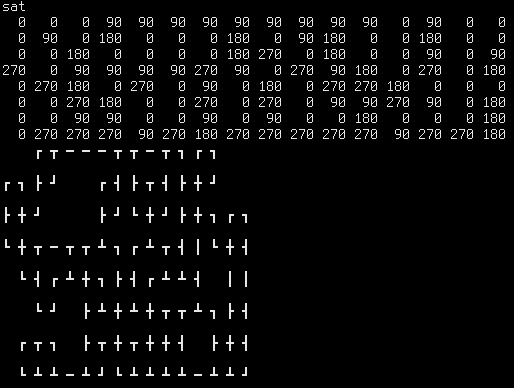
\includegraphics[scale=0.75]{\CURPATH/solver/solver.png}
\caption{Вывод скрипта солвера}
\end{figure}

Это работает $\approx 4$ секунды на моем старом и медленном Intel Atom N455 1.66GHz.
Быстро ли это? Не знаю, но снова вот что действительно круто, это то что мы понятия не имеем о какой-то математической
теории за всем этим, мы просто объявили ячейки, (полу-)стыки и определили отношения между ними.

Теперь следующий вопрос это, сколько здесь возможных решений?
Используя раннее описанный метод (\ref{SMTEnumerate}), я немного изменил скрипт солвера
\footnote{\url{.../solver/solve_pipe_puzzle2.py}} и солвер
сказал что возможно два решения.

Сравним их используя gvimdiff:

\begin{figure}[H]
\centering
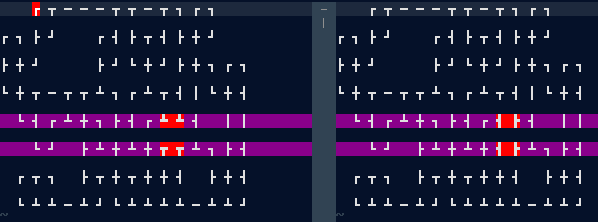
\includegraphics[scale=0.75]{\CURPATH/solver/diff.png}
\caption{Вывод gvimdiff (извините за мой красный курсор в левой части в левом верхнем углу)}
\end{figure}

4 ячейки в середине могут быть ориентированы по-разному.
Видимо, другие головоломки могут также выдавать разные результаты.

P.S.
\textit{Полу-стык} определен как булевый тип.
Но на самом деле, первая версия солвера была написана используя целочисленный тип для полу-стыков,
и 0 использовалось для False и 1 для True.
Я так сделал, потому что хотел более компактный исходный код, без использования длинных слов как ``False'' и ``True''.
И это работало, но медленнее. Вероятно, Z3 работает с булевыми типами быстрее? Лучше?
Так или иначе, я пишу это чтобы отметить, что, если нужно, целочисленный тип можно использовать вместо булевого.


\section{Развлекательная математика и головоломки}

\input{puzzles/sudoku/main_RU}
\input{puzzles/zebra/main_RU}
\input{puzzles/pipe/main_RU}
\input{puzzles/rubik2/failed_SMT/main_RU}
\input{puzzles/rubik2/SAT/main_RU}
\input{puzzles/rubik3/one_face_SMT/main_RU}
%\input{puzzles/numberlink/main_RU}
%\input{puzzles/two_parks_RU}
\input{puzzles/alphametics/main_RU}
%\input{puzzles/2015_AIME_II_Problems_12_RU}
%\input{puzzles/fred/main_RU}
%\input{puzzles/MC/main_RU}
%\input{puzzles/coin_flip/main_RU}
%\input{puzzles/Mock_AIME_2_2006-2007_Problem_8_RU}
%\input{puzzles/2012_AIME_I_Problems_1_RU}
%\input{puzzles/keypad_RU}


\section{Развлекательная математика и головоломки}

\input{puzzles/sudoku/main_RU}
\input{puzzles/zebra/main_RU}
\input{puzzles/pipe/main_RU}
\input{puzzles/rubik2/failed_SMT/main_RU}
\input{puzzles/rubik2/SAT/main_RU}
\input{puzzles/rubik3/one_face_SMT/main_RU}
%\input{puzzles/numberlink/main_RU}
%\input{puzzles/two_parks_RU}
\input{puzzles/alphametics/main_RU}
%\input{puzzles/2015_AIME_II_Problems_12_RU}
%\input{puzzles/fred/main_RU}
%\input{puzzles/MC/main_RU}
%\input{puzzles/coin_flip/main_RU}
%\input{puzzles/Mock_AIME_2_2006-2007_Problem_8_RU}
%\input{puzzles/2012_AIME_I_Problems_1_RU}
%\input{puzzles/keypad_RU}


\section{Развлекательная математика и головоломки}

\input{puzzles/sudoku/main_RU}
\input{puzzles/zebra/main_RU}
\input{puzzles/pipe/main_RU}
\input{puzzles/rubik2/failed_SMT/main_RU}
\input{puzzles/rubik2/SAT/main_RU}
\input{puzzles/rubik3/one_face_SMT/main_RU}
%\input{puzzles/numberlink/main_RU}
%\input{puzzles/two_parks_RU}
\input{puzzles/alphametics/main_RU}
%\input{puzzles/2015_AIME_II_Problems_12_RU}
%\input{puzzles/fred/main_RU}
%\input{puzzles/MC/main_RU}
%\input{puzzles/coin_flip/main_RU}
%\input{puzzles/Mock_AIME_2_2006-2007_Problem_8_RU}
%\input{puzzles/2012_AIME_I_Problems_1_RU}
%\input{puzzles/keypad_RU}


%\section{Развлекательная математика и головоломки}

\input{puzzles/sudoku/main_RU}
\input{puzzles/zebra/main_RU}
\input{puzzles/pipe/main_RU}
\input{puzzles/rubik2/failed_SMT/main_RU}
\input{puzzles/rubik2/SAT/main_RU}
\input{puzzles/rubik3/one_face_SMT/main_RU}
%\input{puzzles/numberlink/main_RU}
%\input{puzzles/two_parks_RU}
\input{puzzles/alphametics/main_RU}
%\input{puzzles/2015_AIME_II_Problems_12_RU}
%\input{puzzles/fred/main_RU}
%\input{puzzles/MC/main_RU}
%\input{puzzles/coin_flip/main_RU}
%\input{puzzles/Mock_AIME_2_2006-2007_Problem_8_RU}
%\input{puzzles/2012_AIME_I_Problems_1_RU}
%\input{puzzles/keypad_RU}


%\input{puzzles/two_parks_RU}
\subsection{Альфаметика}

Согласно Дональду Кнуту, термин ``Альфаметика'' был придуман Дж. Эйч. Аш. Хантером.
Это головоломка: какие десятичные цифры в пределах 0..9 нужно присвоить каждой букве, чтобы это уравнение было справедливо?

\begin{lstlisting}
  SEND
+ MORE
 -----
 MONEY
\end{lstlisting}

Для Z3 это легко:

\lstinputlisting{puzzles/alphametics/alpha.py}

Вывод:

\begin{lstlisting}
sat
[E, = 5,
 S, = 9,
 M, = 1,
 N, = 6,
 D, = 7,
 R, = 8,
 O, = 0,
 Y = 2]
\end{lstlisting}

Вот еще одна, из \ac{TAOCP} том IV (\url{http://www-cs-faculty.stanford.edu/~uno/fasc2b.ps.gz}):

\lstinputlisting{puzzles/alphametics/alpha2.py}

\begin{lstlisting}
sat
[L, = 6,
 S, = 7,
 N, = 2,
 T, = 1,
 I, = 5,
 V = 3,
 A, = 8,
 R, = 9,
 O, = 4,
 TRIO = 1954,
 SONATA, = 742818,
 VIOLA, = 35468,
 VIOLIN, = 354652]
\end{lstlisting}

% TODO URL
Эту головоломку я нашел в примерах pySMT:

\lstinputlisting{puzzles/alphametics/alpha3.py}

\begin{lstlisting}
sat
[D = 5, R = 4, O = 3, E = 8, L = 6, W = 7, H = 2]
\end{lstlisting}

%%% 

Это упражнение Q209 из
[Companion to the Papers of Donald Knuth]\footnote{\url{http://www-cs-faculty.stanford.edu/~knuth/cp.html}}.

\begin{lstlisting}
 KNIFE
  FORK
 SPOON
  SOUP
------
SUPPER
\end{lstlisting}

В целях упрощения, я добавил ф-цию (list\_to\_expr()):

\lstinputlisting{puzzles/alphametics/alpha4.py}

\begin{lstlisting}
sat
[K = 7,
 N = 4,
 R = 9,
 I = 1,
 E = 6,
 S = 0,
 O = 3,
 F = 5,
 U = 8,
 P = 2,
 SUPPER = 82269,
 SOUP = 382,
 SPOON = 2334,
 FORK = 5397,
 KNIFE = 74156]
\end{lstlisting}

S это 0, так что значение SUPPER начинается с (убранного) нуля. Скажем так, нам это не нравится.
Добавим это, чтобы это исправить:

\begin{lstlisting}
s.add(S!=0)
\end{lstlisting}

\begin{lstlisting}
sat
[K = 8,
 N = 4,
 R = 3,
 I = 7,
 E = 6,
 S = 1,
 O = 9,
 F = 2,
 U = 0,
 P = 5,
 SUPPER = 105563,
 SOUP = 1905,
 SPOON = 15994,
 FORK = 2938,
 KNIFE = 84726]
\end{lstlisting}

\paragraph{Создание своей собственной головоломки}

Вот проблема: есть только 10 букв, но как их выбрать из числа слов?
Мы можем использовать Z3 для этого:

\lstinputlisting{puzzles/alphametics/gen.py}

Это первая сгенерированная головоломка:

\begin{lstlisting}
sat
EGGS
JELLY
LUNCH
C 5
E 6
G 3
H 7
J 0
L 1
N 4
S 8
U 2
Y 9
\end{lstlisting}

Что если мы хотим, чтобы слово ``CAKE'' присутствовало в числе ``слагаемых''?

Добавим это:

\begin{lstlisting}
s.add(word_used[words.index('CAKE')])
\end{lstlisting}

\begin{lstlisting}
sat
CAKE
TEA
LUNCH
A 8
C 3
E 1
H 9
J 6
K 2
L 0
N 5
T 7
U 4
\end{lstlisting}

Добавим это:

\begin{lstlisting}
s.add(word_used[words.index('EGGS')])
\end{lstlisting}

Теперь оно может найти пару к EGGS:

\begin{lstlisting}
sat
EGGS
HONEY
LUNCH
C 6
E 7
G 9
H 4
L 5
N 8
O 2
S 3
U 0
Y 1
\end{lstlisting}

\paragraph{Файлы}

\url{https://github.com/DennisYurichev/...}




%\input{puzzles/2015_AIME_II_Problems_12_RU}
%\section{Развлекательная математика и головоломки}

\input{puzzles/sudoku/main_RU}
\input{puzzles/zebra/main_RU}
\input{puzzles/pipe/main_RU}
\input{puzzles/rubik2/failed_SMT/main_RU}
\input{puzzles/rubik2/SAT/main_RU}
\input{puzzles/rubik3/one_face_SMT/main_RU}
%\input{puzzles/numberlink/main_RU}
%\input{puzzles/two_parks_RU}
\input{puzzles/alphametics/main_RU}
%\input{puzzles/2015_AIME_II_Problems_12_RU}
%\input{puzzles/fred/main_RU}
%\input{puzzles/MC/main_RU}
%\input{puzzles/coin_flip/main_RU}
%\input{puzzles/Mock_AIME_2_2006-2007_Problem_8_RU}
%\input{puzzles/2012_AIME_I_Problems_1_RU}
%\input{puzzles/keypad_RU}


%\section{Развлекательная математика и головоломки}

\input{puzzles/sudoku/main_RU}
\input{puzzles/zebra/main_RU}
\input{puzzles/pipe/main_RU}
\input{puzzles/rubik2/failed_SMT/main_RU}
\input{puzzles/rubik2/SAT/main_RU}
\input{puzzles/rubik3/one_face_SMT/main_RU}
%\input{puzzles/numberlink/main_RU}
%\input{puzzles/two_parks_RU}
\input{puzzles/alphametics/main_RU}
%\input{puzzles/2015_AIME_II_Problems_12_RU}
%\input{puzzles/fred/main_RU}
%\input{puzzles/MC/main_RU}
%\input{puzzles/coin_flip/main_RU}
%\input{puzzles/Mock_AIME_2_2006-2007_Problem_8_RU}
%\input{puzzles/2012_AIME_I_Problems_1_RU}
%\input{puzzles/keypad_RU}


%\section{Развлекательная математика и головоломки}

\input{puzzles/sudoku/main_RU}
\input{puzzles/zebra/main_RU}
\input{puzzles/pipe/main_RU}
\input{puzzles/rubik2/failed_SMT/main_RU}
\input{puzzles/rubik2/SAT/main_RU}
\input{puzzles/rubik3/one_face_SMT/main_RU}
%\input{puzzles/numberlink/main_RU}
%\input{puzzles/two_parks_RU}
\input{puzzles/alphametics/main_RU}
%\input{puzzles/2015_AIME_II_Problems_12_RU}
%\input{puzzles/fred/main_RU}
%\input{puzzles/MC/main_RU}
%\input{puzzles/coin_flip/main_RU}
%\input{puzzles/Mock_AIME_2_2006-2007_Problem_8_RU}
%\input{puzzles/2012_AIME_I_Problems_1_RU}
%\input{puzzles/keypad_RU}


%\input{puzzles/Mock_AIME_2_2006-2007_Problem_8_RU}
%\input{puzzles/2012_AIME_I_Problems_1_RU}
%\input{puzzles/keypad_RU}


%\section{Развлекательная математика и головоломки}

\subsection{Судоку}

Головоломка Судоку это решетка 9*9, некоторые ячейки заполнены значениями, некоторые пустые:

% copypasted from http://www.texample.net/tikz/examples/sudoku/
\newcounter{row}
\newcounter{col}

\newcommand\setrow[9]{
  \setcounter{col}{1}
  \foreach \n in {#1, #2, #3, #4, #5, #6, #7, #8, #9} {
    \edef\x{\value{col} - 0.5}
    \edef\y{9.5 - \value{row}}
    \node[anchor=center] at (\x, \y) {\n};
    \stepcounter{col}
  }
  \stepcounter{row}
}

\begin{center}
\begin{tikzpicture}[scale=.7]
  \begin{scope}
    \draw (0, 0) grid (9, 9);
    \draw[very thick, scale=3] (0, 0) grid (3, 3);

    \setcounter{row}{1}
    \setrow { }{ }{5}  {3}{ }{ }  { }{ }{ }
    \setrow {8}{ }{ }  { }{ }{ }  { }{2}{ }
    \setrow { }{7}{ }  { }{1}{ }  {5}{ }{ }

    \setrow {4}{ }{ }  { }{ }{5}  {3}{ }{ }
    \setrow { }{1}{ }  { }{7}{ }  { }{ }{6}
    \setrow { }{ }{3}  {2}{ }{ }  { }{8}{ }

    \setrow { }{6}{ }  {5}{ }{ }  { }{ }{9}
    \setrow { }{ }{4}  { }{ }{ }  { }{3}{ }
    \setrow { }{ }{ }  { }{ }{9}  {7}{ }{ }

    \node[anchor=center] at (4.5, -0.5) {Нерешенная Судоку};
  \end{scope}
\end{tikzpicture}
\end{center}

Числа в каждом ряду должны быть уникальными, т.е., каждый ряд должен содержать 9 чисел в пределах 1..9 без повторений.
Та же история и для каждого столбца и каждого квадрата 3*3.

Головоломка представляет собой хороший кандидат, на котором можно попробовать \ac{SMT}-солвер, потому что это,
в общем-то, просто нерешенная система уравнений.

\input{puzzles/sudoku/1/main_RU}
%\input{puzzles/sudoku/GT/main_RU}
%\input{puzzles/sudoku/killer/main_RU}
\input{puzzles/sudoku/KLEE/main_RU}
\input{puzzles/sudoku/SAT/main_RU}


\subsection{Головоломка зебры (\ac{AKA} Загадка Эйнштейна)}

\input{puzzles/zebra/SMT/main_RU}
\input{puzzles/zebra/KLEE/main_RU}
\input{puzzles/zebra/SAT/main_RU}


\subsection{Решение головоломки ``трубы'' используя Z3 SMT-солвер}

\renewcommand{\CURPATH}{puzzles/pipe}

Головоломка ``трубы'' это популярная головоломка (просто погуглите ``pipe puzzle'' и посмотрите на картинки).

Вот как выглядит головоломка в разобранном виде:

\begin{figure}[H]
\label{fig:pipe_shuffled}
\centering
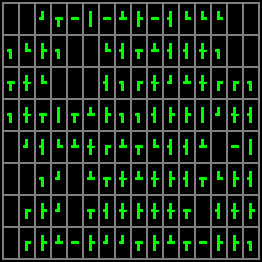
\includegraphics[scale=0.75]{\CURPATH/shuffled.png}
\caption{Разобранная головоломка}
\end{figure}

\dots и собранная:

\begin{figure}[H]
\label{fig:pipe_solved}
\centering
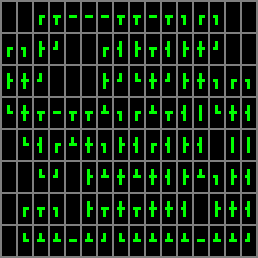
\includegraphics[scale=0.75]{\CURPATH/solved.png}
\caption{Собранная головоломка}
\end{figure}

Попробуем найти способ собрать её.

\subsubsection{Создание}

В начале, нужно её создать.
Вот простая идея.
Возьем массив ячеек 8*16.
Каждая ячейка может содержать какой-то тип блока.
Между ячейками есть стыки:

\input{\CURPATH/pipe_gen.tex}

Синие линии это горизонтальные стыки, красные линии это вертикальные стыки.
Мы просто случайно выставляем каждый стык в 0/false (отсутствует) или 1/true (присутствует).

После этого, теперь легко найти тип каждой ячейки.
А это:

\newcommand{\HeaderColor}{\cellcolor{blue!25}}
\begin{center}
\begin{longtable}{ | l | l | l | l | }
\hline
\HeaderColor стыки & \HeaderColor наше внутреннее название & \HeaderColor угол & \HeaderColor символ \\
\hline
0	&type 0		&	0$^{\circ}$	& (пробел)	\\
2	&type 2a	&	0$^{\circ}$	& \pmboxdrawuni{2503} \\ % ┃
2	&type 2a	&	90$^{\circ}$	& \pmboxdrawuni{2501} \\ % ━
2	&type 2b	&	0$^{\circ}$	& \pmboxdrawuni{250F} \\ % ┏
2	&type 2b	&	90$^{\circ}$	& \pmboxdrawuni{2513} \\ % ┓
2	&type 2b	&	180$^{\circ}$	& \pmboxdrawuni{251B} \\ % ┛
2	&type 2b	&	270$^{\circ}$	& \pmboxdrawuni{2517} \\ % ┗
3	&type 3		&	0$^{\circ}$	& \pmboxdrawuni{2523} \\ % ┣
3 	&type 3		&	90$^{\circ}$	& \pmboxdrawuni{2533} \\ % ┳
3	&type 3		&	180$^{\circ}$	& \pmboxdrawuni{252B} \\ % ┫
3	&type 3		&	270$^{\circ}$	& \pmboxdrawuni{253B} \\ % ┻
4	&type 4		&	0$^{\circ}$	& \pmboxdrawuni{254B} \\ % ╋
\hline
\end{longtable}
\end{center}

\textit{Висящие} стыки могут присутствовать на первой стадии (т.е., ячейки только с одним стыком), но они удалются
рекурсивно, и эти ячейки преобразуются в пустые ячейки.
Так что, в самом конце, все ячейки имеют минимум 2 стыка, и вся эта сантехническая система не имеет связей с внешним миром ---
я надеюсь, из-за этого станет немного проще.

Исходник генератора на Си здесь: \url{.../pipe/generator}.
Все вертикальные стыки хранятся в глобальном массиве \textit{hjoints[]} и вертикальные в \textit{vjoints[]}.

Программа на Си генерирует ANSI-раскрашенный вывод, как это было показано выше
(\ref{fig:pipe_shuffled}, \ref{fig:pipe_solved}) плюс массив типов для каждой ячейки, но без информации об углах:

\begin{lstlisting}[label=init_cells]
[
["0", "0", "2b", "3", "2a", "2a", "2a", "3", "3", "2a", "3", "2b", "2b", "2b", "0", "0"],
["2b", "2b", "3", "2b", "0", "0", "2b", "3", "3", "3", "3", "3", "4", "2b", "0", "0"],
["3", "4", "2b", "0", "0", "0", "3", "2b", "2b", "4", "2b", "3", "4", "2b", "2b", "2b"],
["2b", "4", "3", "2a", "3", "3", "3", "2b", "2b", "3", "3", "3", "2a", "2b", "4", "3"],
["0", "2b", "3", "2b", "3", "4", "2b", "3", "3", "2b", "3", "3", "3", "0", "2a", "2a"],
["0", "0", "2b", "2b", "0", "3", "3", "4", "3", "4", "3", "3", "3", "2b", "3", "3"],
["0", "2b", "3", "2b", "0", "3", "3", "4", "3", "4", "4", "3", "0", "3", "4", "3"],
["0", "2b", "3", "3", "2a", "3", "2b", "2b", "3", "3", "3", "3", "2a", "3", "3", "2b"],
]
\end{lstlisting}

\subsubsection{Решение}

Прежде всего, мы будем работать с массивом ячеек 8*16, где каждый элемент имеет 4 бита:
``T'' (top/верх),
``B'' (bottom/низ),
``L'' (left/лево),
``R'' (right/право).
Каждый бит представляет собой половину стыка.

\input{\CURPATH/pipe_solve.tex}

Теперь определяем массив для каждого из четырех полустыков + информация об угле:

\begin{lstlisting}
HEIGHT=8
WIDTH=16

# if T/B/R/L is Bool instead of Int, Z3 solver will work faster
T=[[Bool('cell_%d_%d_top' % (r, c)) for c in range(WIDTH)] for r in range(HEIGHT)]
B=[[Bool('cell_%d_%d_bottom' % (r, c)) for c in range(WIDTH)] for r in range(HEIGHT)]
R=[[Bool('cell_%d_%d_right' % (r, c)) for c in range(WIDTH)] for r in range(HEIGHT)]
L=[[Bool('cell_%d_%d_left' % (r, c)) for c in range(WIDTH)] for r in range(HEIGHT)]
A=[[Int('cell_%d_%d_angle' % (r, c)) for c in range(WIDTH)] for r in range(HEIGHT)]
\end{lstlisting}

Мы знаем, что если каждый из полустыков присутствует, ответный полустык также должен присутствовать, и наоборот. 
Определяем всё это используя эти констрайнты:

\begin{lstlisting}
# shorthand variables for True and False:
t=True
f=False

# "top" of each cell must be equal to "bottom" of the cell above
# "bottom" of each cell must be equal to "top" of the cell below
# "left" of each cell must be equal to "right" of the cell at left
# "right" of each cell must be equal to "left" of the cell at right
for r in range(HEIGHT):
    for c in range(WIDTH):
        if r!=0:
            s.add(T[r][c]==B[r-1][c])
        if r!=HEIGHT-1:
            s.add(B[r][c]==T[r+1][c])
        if c!=0:
            s.add(L[r][c]==R[r][c-1])
        if c!=WIDTH-1:
            s.add(R[r][c]==L[r][c+1])

# "left" of each cell of first column shouldn't have any connection
# so is "right" of each cell of the last column
for r in range(HEIGHT):
    s.add(L[r][0]==f)
    s.add(R[r][WIDTH-1]==f)

# "top" of each cell of the first row shouldn't have any connection
# so is "bottom" of each cell of the last row
for c in range(WIDTH):
    s.add(T[0][c]==f)
    s.add(B[HEIGHT-1][c]==f)
\end{lstlisting}

Теперь перебираем все ячейки в изначальном массиве (\ref{init_cells}).
Первые две ячейки здесь пустые. И третья имеет тип ``2b''.
Это ``\pmboxdrawuni{250F}'' % ┏
и его можно ориентировать четырьмя разными способами.
И если её угол это 0$^{\circ}$, верхний и правый полустыки присутствуют, остальные отсутствуют.
Если он имеет угол 90$^{\circ}$, он выглядит как 
``\pmboxdrawuni{2513}'', % ┓
и верхник и левый полустыки присутствуют, остальные отсутствуют.

На обычном русском языке: ``если ячейка этого типа имеет угол 0$^{\circ}$, вот эти полустыки должны присутствовать \textbf{ИЛИ}
если она имеет угол 90$^{\circ}$, эти полустыки должны присутствовать, \textbf{ИЛИ}, итд, итд.''

Точно также, мы определяем эти правила для всех типов и всех возможных углов:

\begin{lstlisting}
for r in range(HEIGHT):
    for c in range(WIDTH):
        ty=cells_type[r][c]

        if ty=="0":
            s.add(A[r][c]==f)
            s.add(T[r][c]==f, B[r][c]==f, L[r][c]==f, R[r][c]==f)

        if ty=="2a":
            s.add(Or(And(A[r][c]==0, L[r][c]==f, R[r][c]==f, T[r][c]==t, B[r][c]==t),   # §\pmboxdrawuni{2503}§
                    And(A[r][c]==90, L[r][c]==t, R[r][c]==t, T[r][c]==f, B[r][c]==f)))  # §\pmboxdrawuni{2501}§

        if ty=="2b":
            s.add(Or(And(A[r][c]==0, L[r][c]==f, R[r][c]==t, T[r][c]==f, B[r][c]==t),   # §\pmboxdrawuni{250F}§
                    And(A[r][c]==90, L[r][c]==t, R[r][c]==f, T[r][c]==f, B[r][c]==t),   # §\pmboxdrawuni{2513}§
                    And(A[r][c]==180, L[r][c]==t, R[r][c]==f, T[r][c]==t, B[r][c]==f),  # §\pmboxdrawuni{251B}§
                    And(A[r][c]==270, L[r][c]==f, R[r][c]==t, T[r][c]==t, B[r][c]==f))) # §\pmboxdrawuni{2517}§
	
        if ty=="3":
            s.add(Or(And(A[r][c]==0, L[r][c]==f, R[r][c]==t, T[r][c]==t, B[r][c]==t),   # §\pmboxdrawuni{2523}§
                    And(A[r][c]==90, L[r][c]==t, R[r][c]==t, T[r][c]==f, B[r][c]==t),   # §\pmboxdrawuni{2533}§
                    And(A[r][c]==180, L[r][c]==t, R[r][c]==f, T[r][c]==t, B[r][c]==t),  # §\pmboxdrawuni{252B}§
                    And(A[r][c]==270, L[r][c]==t, R[r][c]==t, T[r][c]==t, B[r][c]==f))) # §\pmboxdrawuni{253B}§

        if ty=="4":
            s.add(A[r][c]==0)
            s.add(T[r][c]==t, B[r][c]==t, L[r][c]==t, R[r][c]==t) # §\pmboxdrawuni{254B}§
\end{lstlisting}

Полный исходник здесь: \url{.../solver/solve_pipe_puzzle1.py}.

Получается такой результат (выводит угол для каждой ячейки и (псевдо)графическое представление):

\begin{figure}[H]
\centering
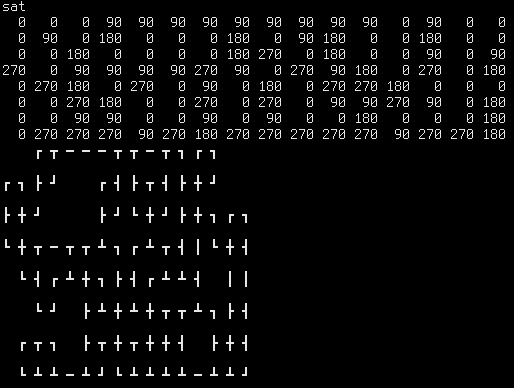
\includegraphics[scale=0.75]{\CURPATH/solver/solver.png}
\caption{Вывод скрипта солвера}
\end{figure}

Это работает $\approx 4$ секунды на моем старом и медленном Intel Atom N455 1.66GHz.
Быстро ли это? Не знаю, но снова вот что действительно круто, это то что мы понятия не имеем о какой-то математической
теории за всем этим, мы просто объявили ячейки, (полу-)стыки и определили отношения между ними.

Теперь следующий вопрос это, сколько здесь возможных решений?
Используя раннее описанный метод (\ref{SMTEnumerate}), я немного изменил скрипт солвера
\footnote{\url{.../solver/solve_pipe_puzzle2.py}} и солвер
сказал что возможно два решения.

Сравним их используя gvimdiff:

\begin{figure}[H]
\centering
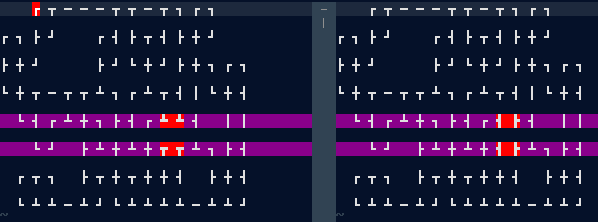
\includegraphics[scale=0.75]{\CURPATH/solver/diff.png}
\caption{Вывод gvimdiff (извините за мой красный курсор в левой части в левом верхнем углу)}
\end{figure}

4 ячейки в середине могут быть ориентированы по-разному.
Видимо, другие головоломки могут также выдавать разные результаты.

P.S.
\textit{Полу-стык} определен как булевый тип.
Но на самом деле, первая версия солвера была написана используя целочисленный тип для полу-стыков,
и 0 использовалось для False и 1 для True.
Я так сделал, потому что хотел более компактный исходный код, без использования длинных слов как ``False'' и ``True''.
И это работало, но медленнее. Вероятно, Z3 работает с булевыми типами быстрее? Лучше?
Так или иначе, я пишу это чтобы отметить, что, если нужно, целочисленный тип можно использовать вместо булевого.


\section{Развлекательная математика и головоломки}

\input{puzzles/sudoku/main_RU}
\input{puzzles/zebra/main_RU}
\input{puzzles/pipe/main_RU}
\input{puzzles/rubik2/failed_SMT/main_RU}
\input{puzzles/rubik2/SAT/main_RU}
\input{puzzles/rubik3/one_face_SMT/main_RU}
%\input{puzzles/numberlink/main_RU}
%\input{puzzles/two_parks_RU}
\input{puzzles/alphametics/main_RU}
%\input{puzzles/2015_AIME_II_Problems_12_RU}
%\input{puzzles/fred/main_RU}
%\input{puzzles/MC/main_RU}
%\input{puzzles/coin_flip/main_RU}
%\input{puzzles/Mock_AIME_2_2006-2007_Problem_8_RU}
%\input{puzzles/2012_AIME_I_Problems_1_RU}
%\input{puzzles/keypad_RU}


\section{Развлекательная математика и головоломки}

\input{puzzles/sudoku/main_RU}
\input{puzzles/zebra/main_RU}
\input{puzzles/pipe/main_RU}
\input{puzzles/rubik2/failed_SMT/main_RU}
\input{puzzles/rubik2/SAT/main_RU}
\input{puzzles/rubik3/one_face_SMT/main_RU}
%\input{puzzles/numberlink/main_RU}
%\input{puzzles/two_parks_RU}
\input{puzzles/alphametics/main_RU}
%\input{puzzles/2015_AIME_II_Problems_12_RU}
%\input{puzzles/fred/main_RU}
%\input{puzzles/MC/main_RU}
%\input{puzzles/coin_flip/main_RU}
%\input{puzzles/Mock_AIME_2_2006-2007_Problem_8_RU}
%\input{puzzles/2012_AIME_I_Problems_1_RU}
%\input{puzzles/keypad_RU}


\section{Развлекательная математика и головоломки}

\input{puzzles/sudoku/main_RU}
\input{puzzles/zebra/main_RU}
\input{puzzles/pipe/main_RU}
\input{puzzles/rubik2/failed_SMT/main_RU}
\input{puzzles/rubik2/SAT/main_RU}
\input{puzzles/rubik3/one_face_SMT/main_RU}
%\input{puzzles/numberlink/main_RU}
%\input{puzzles/two_parks_RU}
\input{puzzles/alphametics/main_RU}
%\input{puzzles/2015_AIME_II_Problems_12_RU}
%\input{puzzles/fred/main_RU}
%\input{puzzles/MC/main_RU}
%\input{puzzles/coin_flip/main_RU}
%\input{puzzles/Mock_AIME_2_2006-2007_Problem_8_RU}
%\input{puzzles/2012_AIME_I_Problems_1_RU}
%\input{puzzles/keypad_RU}


%\section{Развлекательная математика и головоломки}

\input{puzzles/sudoku/main_RU}
\input{puzzles/zebra/main_RU}
\input{puzzles/pipe/main_RU}
\input{puzzles/rubik2/failed_SMT/main_RU}
\input{puzzles/rubik2/SAT/main_RU}
\input{puzzles/rubik3/one_face_SMT/main_RU}
%\input{puzzles/numberlink/main_RU}
%\input{puzzles/two_parks_RU}
\input{puzzles/alphametics/main_RU}
%\input{puzzles/2015_AIME_II_Problems_12_RU}
%\input{puzzles/fred/main_RU}
%\input{puzzles/MC/main_RU}
%\input{puzzles/coin_flip/main_RU}
%\input{puzzles/Mock_AIME_2_2006-2007_Problem_8_RU}
%\input{puzzles/2012_AIME_I_Problems_1_RU}
%\input{puzzles/keypad_RU}


%\input{puzzles/two_parks_RU}
\subsection{Альфаметика}

Согласно Дональду Кнуту, термин ``Альфаметика'' был придуман Дж. Эйч. Аш. Хантером.
Это головоломка: какие десятичные цифры в пределах 0..9 нужно присвоить каждой букве, чтобы это уравнение было справедливо?

\begin{lstlisting}
  SEND
+ MORE
 -----
 MONEY
\end{lstlisting}

Для Z3 это легко:

\lstinputlisting{puzzles/alphametics/alpha.py}

Вывод:

\begin{lstlisting}
sat
[E, = 5,
 S, = 9,
 M, = 1,
 N, = 6,
 D, = 7,
 R, = 8,
 O, = 0,
 Y = 2]
\end{lstlisting}

Вот еще одна, из \ac{TAOCP} том IV (\url{http://www-cs-faculty.stanford.edu/~uno/fasc2b.ps.gz}):

\lstinputlisting{puzzles/alphametics/alpha2.py}

\begin{lstlisting}
sat
[L, = 6,
 S, = 7,
 N, = 2,
 T, = 1,
 I, = 5,
 V = 3,
 A, = 8,
 R, = 9,
 O, = 4,
 TRIO = 1954,
 SONATA, = 742818,
 VIOLA, = 35468,
 VIOLIN, = 354652]
\end{lstlisting}

% TODO URL
Эту головоломку я нашел в примерах pySMT:

\lstinputlisting{puzzles/alphametics/alpha3.py}

\begin{lstlisting}
sat
[D = 5, R = 4, O = 3, E = 8, L = 6, W = 7, H = 2]
\end{lstlisting}

%%% 

Это упражнение Q209 из
[Companion to the Papers of Donald Knuth]\footnote{\url{http://www-cs-faculty.stanford.edu/~knuth/cp.html}}.

\begin{lstlisting}
 KNIFE
  FORK
 SPOON
  SOUP
------
SUPPER
\end{lstlisting}

В целях упрощения, я добавил ф-цию (list\_to\_expr()):

\lstinputlisting{puzzles/alphametics/alpha4.py}

\begin{lstlisting}
sat
[K = 7,
 N = 4,
 R = 9,
 I = 1,
 E = 6,
 S = 0,
 O = 3,
 F = 5,
 U = 8,
 P = 2,
 SUPPER = 82269,
 SOUP = 382,
 SPOON = 2334,
 FORK = 5397,
 KNIFE = 74156]
\end{lstlisting}

S это 0, так что значение SUPPER начинается с (убранного) нуля. Скажем так, нам это не нравится.
Добавим это, чтобы это исправить:

\begin{lstlisting}
s.add(S!=0)
\end{lstlisting}

\begin{lstlisting}
sat
[K = 8,
 N = 4,
 R = 3,
 I = 7,
 E = 6,
 S = 1,
 O = 9,
 F = 2,
 U = 0,
 P = 5,
 SUPPER = 105563,
 SOUP = 1905,
 SPOON = 15994,
 FORK = 2938,
 KNIFE = 84726]
\end{lstlisting}

\paragraph{Создание своей собственной головоломки}

Вот проблема: есть только 10 букв, но как их выбрать из числа слов?
Мы можем использовать Z3 для этого:

\lstinputlisting{puzzles/alphametics/gen.py}

Это первая сгенерированная головоломка:

\begin{lstlisting}
sat
EGGS
JELLY
LUNCH
C 5
E 6
G 3
H 7
J 0
L 1
N 4
S 8
U 2
Y 9
\end{lstlisting}

Что если мы хотим, чтобы слово ``CAKE'' присутствовало в числе ``слагаемых''?

Добавим это:

\begin{lstlisting}
s.add(word_used[words.index('CAKE')])
\end{lstlisting}

\begin{lstlisting}
sat
CAKE
TEA
LUNCH
A 8
C 3
E 1
H 9
J 6
K 2
L 0
N 5
T 7
U 4
\end{lstlisting}

Добавим это:

\begin{lstlisting}
s.add(word_used[words.index('EGGS')])
\end{lstlisting}

Теперь оно может найти пару к EGGS:

\begin{lstlisting}
sat
EGGS
HONEY
LUNCH
C 6
E 7
G 9
H 4
L 5
N 8
O 2
S 3
U 0
Y 1
\end{lstlisting}

\paragraph{Файлы}

\url{https://github.com/DennisYurichev/...}




%\input{puzzles/2015_AIME_II_Problems_12_RU}
%\section{Развлекательная математика и головоломки}

\input{puzzles/sudoku/main_RU}
\input{puzzles/zebra/main_RU}
\input{puzzles/pipe/main_RU}
\input{puzzles/rubik2/failed_SMT/main_RU}
\input{puzzles/rubik2/SAT/main_RU}
\input{puzzles/rubik3/one_face_SMT/main_RU}
%\input{puzzles/numberlink/main_RU}
%\input{puzzles/two_parks_RU}
\input{puzzles/alphametics/main_RU}
%\input{puzzles/2015_AIME_II_Problems_12_RU}
%\input{puzzles/fred/main_RU}
%\input{puzzles/MC/main_RU}
%\input{puzzles/coin_flip/main_RU}
%\input{puzzles/Mock_AIME_2_2006-2007_Problem_8_RU}
%\input{puzzles/2012_AIME_I_Problems_1_RU}
%\input{puzzles/keypad_RU}


%\section{Развлекательная математика и головоломки}

\input{puzzles/sudoku/main_RU}
\input{puzzles/zebra/main_RU}
\input{puzzles/pipe/main_RU}
\input{puzzles/rubik2/failed_SMT/main_RU}
\input{puzzles/rubik2/SAT/main_RU}
\input{puzzles/rubik3/one_face_SMT/main_RU}
%\input{puzzles/numberlink/main_RU}
%\input{puzzles/two_parks_RU}
\input{puzzles/alphametics/main_RU}
%\input{puzzles/2015_AIME_II_Problems_12_RU}
%\input{puzzles/fred/main_RU}
%\input{puzzles/MC/main_RU}
%\input{puzzles/coin_flip/main_RU}
%\input{puzzles/Mock_AIME_2_2006-2007_Problem_8_RU}
%\input{puzzles/2012_AIME_I_Problems_1_RU}
%\input{puzzles/keypad_RU}


%\section{Развлекательная математика и головоломки}

\input{puzzles/sudoku/main_RU}
\input{puzzles/zebra/main_RU}
\input{puzzles/pipe/main_RU}
\input{puzzles/rubik2/failed_SMT/main_RU}
\input{puzzles/rubik2/SAT/main_RU}
\input{puzzles/rubik3/one_face_SMT/main_RU}
%\input{puzzles/numberlink/main_RU}
%\input{puzzles/two_parks_RU}
\input{puzzles/alphametics/main_RU}
%\input{puzzles/2015_AIME_II_Problems_12_RU}
%\input{puzzles/fred/main_RU}
%\input{puzzles/MC/main_RU}
%\input{puzzles/coin_flip/main_RU}
%\input{puzzles/Mock_AIME_2_2006-2007_Problem_8_RU}
%\input{puzzles/2012_AIME_I_Problems_1_RU}
%\input{puzzles/keypad_RU}


%\input{puzzles/Mock_AIME_2_2006-2007_Problem_8_RU}
%\input{puzzles/2012_AIME_I_Problems_1_RU}
%\input{puzzles/keypad_RU}


%\input{puzzles/Mock_AIME_2_2006-2007_Problem_8_RU}
%\input{puzzles/2012_AIME_I_Problems_1_RU}
%\input{puzzles/keypad_RU}


\section{Развлекательная математика и головоломки}

\subsection{Судоку}

Головоломка Судоку это решетка 9*9, некоторые ячейки заполнены значениями, некоторые пустые:

% copypasted from http://www.texample.net/tikz/examples/sudoku/
\newcounter{row}
\newcounter{col}

\newcommand\setrow[9]{
  \setcounter{col}{1}
  \foreach \n in {#1, #2, #3, #4, #5, #6, #7, #8, #9} {
    \edef\x{\value{col} - 0.5}
    \edef\y{9.5 - \value{row}}
    \node[anchor=center] at (\x, \y) {\n};
    \stepcounter{col}
  }
  \stepcounter{row}
}

\begin{center}
\begin{tikzpicture}[scale=.7]
  \begin{scope}
    \draw (0, 0) grid (9, 9);
    \draw[very thick, scale=3] (0, 0) grid (3, 3);

    \setcounter{row}{1}
    \setrow { }{ }{5}  {3}{ }{ }  { }{ }{ }
    \setrow {8}{ }{ }  { }{ }{ }  { }{2}{ }
    \setrow { }{7}{ }  { }{1}{ }  {5}{ }{ }

    \setrow {4}{ }{ }  { }{ }{5}  {3}{ }{ }
    \setrow { }{1}{ }  { }{7}{ }  { }{ }{6}
    \setrow { }{ }{3}  {2}{ }{ }  { }{8}{ }

    \setrow { }{6}{ }  {5}{ }{ }  { }{ }{9}
    \setrow { }{ }{4}  { }{ }{ }  { }{3}{ }
    \setrow { }{ }{ }  { }{ }{9}  {7}{ }{ }

    \node[anchor=center] at (4.5, -0.5) {Нерешенная Судоку};
  \end{scope}
\end{tikzpicture}
\end{center}

Числа в каждом ряду должны быть уникальными, т.е., каждый ряд должен содержать 9 чисел в пределах 1..9 без повторений.
Та же история и для каждого столбца и каждого квадрата 3*3.

Головоломка представляет собой хороший кандидат, на котором можно попробовать \ac{SMT}-солвер, потому что это,
в общем-то, просто нерешенная система уравнений.

\subsubsection{Простая Судоку и SMT}
\label{sudoku_SMT}

\paragraph{Первая идея}

Всё что нужно решить, это как определять в одном выражении, содержат ли 9 переменных все 9 уникальных чисел?
Они ведь не упорядочены и не отсортированы, все-таки.

Из школьной арифметики, мы можем найти такую идею:

\begin{equation}
\underbrace{10^{i_1} + 10^{i_2} + \cdots + 10^{i_9}}_9 = 1111111110
\end{equation}

Берете каждую входную переменную, вычисляете $10^i$ и суммируете.
Если все входные значения уникальны, каждая найдет свое собственное место.
И даже более того: не будет дыр, т.е., не будет пропущенных значений.
Так что, в случае Судоку, число 1111111110 будет конечным результатом, означающим, что все входные
9 переменных уникальны, в пределах 1..9.

Возведение в степень это тяжелая операция, можно ли использовать двоичные операции? Да, просто замените 10 на 2:

\begin{equation}
\underbrace{2^{i_1} + 2^{i_2} + \cdots + 2^{i_9}}_9 = 1111111110_2
\end{equation}

Эффект тот же, но результат будет в двоичной системе а не в десятичной.

Вот рабочий пример:

\lstinputlisting{puzzles/sudoku/1/sudoku_plus.py}
( \url{https://github.com/DennisYurichev/SAT_SMT_article/.../sudoku_plus.py} )

\begin{lstlisting}
% time python sudoku_plus.py
1 4 5 3 2 7 6 9 8
8 3 9 6 5 4 1 2 7
6 7 2 9 1 8 5 4 3
4 9 6 1 8 5 3 7 2
2 1 8 4 7 3 9 5 6
7 5 3 2 9 6 4 8 1
3 6 7 5 4 2 8 1 9
9 8 4 7 6 1 2 3 5
5 2 1 8 3 9 7 6 4

real    0m11.717s
user    0m10.896s
sys     0m0.068s
\end{lstlisting}

И даже более того, можно заменить суммирование на логическое ИЛИ:

\begin{equation}
\underbrace{2^{i_1} \vee 2^{i_2} \vee \cdots \vee 2^{i_9}}_9 = 1111111110_2
\end{equation}

% FIXME: только часть исходника
\lstinputlisting{puzzles/sudoku/1/sudoku_or.py}
( \url{https://github.com/DennisYurichev/SAT_SMT_article/.../sudoku_or.py} )

Теперь работает намного быстрее. Наверное, Z3 лучше поддерживает операцию ИЛИ над битовыми векторами, чем сложение?

\begin{lstlisting}
% time python sudoku_or.py
1 4 5 3 2 7 6 9 8
8 3 9 6 5 4 1 2 7
6 7 2 9 1 8 5 4 3
4 9 6 1 8 5 3 7 2
2 1 8 4 7 3 9 5 6
7 5 3 2 9 6 4 8 1
3 6 7 5 4 2 8 1 9
9 8 4 7 6 1 2 3 5
5 2 1 8 3 9 7 6 4

real    0m1.429s
user    0m1.393s
sys     0m0.036s
\end{lstlisting}

Головоломка, которую я использовал как пример, известна как самая трудная из известных
\footnote{\url{http://www.mirror.co.uk/news/weird-news/worlds-hardest-sudoku-can-you-242294}} (по крайней мере для людей).
Для решения понадобилось $\approx 1.4$ секунды на моем ноутбуке Intel Core i3-3110M 2.4GHz.

\paragraph{Вторая идея}

Мой первый подход далек от эффективного, я сделал то что первым пришло в голову, и оно заработало.
Другой подход это использовать команду \TT{distinct} в SMT-LIB, которая говорит Z3, что некоторые переменные
должны быть отличны друг от друга (или уникальны).
Эта команда также имеется в питоновском интерфейсе к Z3.

Я переписал мой первый солвер Судоку, теперь он работает над \textit{sort}-ом 
\textit{Int}, и имеет команды \TT{distinct} вместо битовых операций,
и еще один констрайнт добавлен: значение каждой ячейки должно быть в пределах 1..9, потому что, иначе, Z3 предложит
(хотя и корректное) решение с очень большими и/или отрицательными числами.

% FIXME: только часть исходника
\lstinputlisting{puzzles/sudoku/1/sudoku2.py}
( \url{https://github.com/DennisYurichev/SAT_SMT_article/.../sudoku2.py} )

\begin{lstlisting}
% time python sudoku2.py
1 4 5 3 2 7 6 9 8
8 3 9 6 5 4 1 2 7
6 7 2 9 1 8 5 4 3
4 9 6 1 8 5 3 7 2
2 1 8 4 7 3 9 5 6
7 5 3 2 9 6 4 8 1
3 6 7 5 4 2 8 1 9
9 8 4 7 6 1 2 3 5
5 2 1 8 3 9 7 6 4

real    0m0.382s
user    0m0.346s
sys     0m0.036s
\end{lstlisting}

Это намного быстрее.

\paragraph{Вывод}

\ac{SMT}-солверы настолько удобны, что в нашем солвере Судоку нет ничего больше ничего, мы просто определили
отношения между переменными (ячейками).

\paragraph{Домашная работа}

Как видно, настоящая головоломка Судоку это та, для которой имеется только одно решение.
Фрагмент кода, который приведен здесь, показывает только первое.
Использая метод описанный раннее (\ref{SMTEnumerate}, также называемый ``подсчет моделей (model counting)''), 
попытайтесь найти больше решений, или доказать, что решение, которое вы нашли, единственное возможное.

\paragraph{Дальнейшее чтение}

\url{http://www.norvig.com/sudoku.html}

\paragraph{Судоку как \ac{SAT}-проблема}

Головоломку Судоку можно также представить как огромное \ac{CNF}-уравнение и использовать \ac{SAT}-солвер для поиска решения,
но это просто сложнее.

Некоторые статьи об этом:
\textit{Building a Sudoku Solver with SAT}\footnote{\url{http://ocw.mit.edu/courses/electrical-engineering-and-computer-science/6-005-elements-of-software-construction-fall-2011/assignments/MIT6_005F11_ps4.pdf}},
Tjark Weber, \textit{A SAT-based Sudoku Solver}\footnote{\url{https://www.lri.fr/~conchon/mpri/weber.pdf}},
Ines Lynce, Joel Ouaknine, \textit{Sudoku as a SAT Problem}\footnote{\url{http://sat.inesc-id.pt/~ines/publications/aimath06.pdf}},
Gihwon Kwon, Himanshu Jain, \textit{Optimized CNF Encoding for Sudoku Puzzles}\footnote{\url{http://www.cs.cmu.edu/~hjain/papers/sudoku-as-SAT.pdf}}.

\ac{SMT}-солвер также может использовать \ac{SAT}-солвер в своем ядре, так что он делает всю эту скучную работу
по трансляции.
Хотя и, как и компилятор, он может это делать не самым эффективным способом.


%\section{Развлекательная математика и головоломки}

\input{puzzles/sudoku/main_RU}
\input{puzzles/zebra/main_RU}
\input{puzzles/pipe/main_RU}
\input{puzzles/rubik2/failed_SMT/main_RU}
\input{puzzles/rubik2/SAT/main_RU}
\input{puzzles/rubik3/one_face_SMT/main_RU}
%\input{puzzles/numberlink/main_RU}
%\input{puzzles/two_parks_RU}
\input{puzzles/alphametics/main_RU}
%\input{puzzles/2015_AIME_II_Problems_12_RU}
%\input{puzzles/fred/main_RU}
%\input{puzzles/MC/main_RU}
%\input{puzzles/coin_flip/main_RU}
%\input{puzzles/Mock_AIME_2_2006-2007_Problem_8_RU}
%\input{puzzles/2012_AIME_I_Problems_1_RU}
%\input{puzzles/keypad_RU}


%\section{Развлекательная математика и головоломки}

\input{puzzles/sudoku/main_RU}
\input{puzzles/zebra/main_RU}
\input{puzzles/pipe/main_RU}
\input{puzzles/rubik2/failed_SMT/main_RU}
\input{puzzles/rubik2/SAT/main_RU}
\input{puzzles/rubik3/one_face_SMT/main_RU}
%\input{puzzles/numberlink/main_RU}
%\input{puzzles/two_parks_RU}
\input{puzzles/alphametics/main_RU}
%\input{puzzles/2015_AIME_II_Problems_12_RU}
%\input{puzzles/fred/main_RU}
%\input{puzzles/MC/main_RU}
%\input{puzzles/coin_flip/main_RU}
%\input{puzzles/Mock_AIME_2_2006-2007_Problem_8_RU}
%\input{puzzles/2012_AIME_I_Problems_1_RU}
%\input{puzzles/keypad_RU}


\subsubsection{Судоку}

Я также переписал пример с Судоку (\ref{sudoku_SMT}) для KLEE:

\lstinputlisting[numbers=left]{puzzles/sudoku/KLEE/klee_sudoku_or1.c}

Запустим:

\begin{lstlisting}
% clang -emit-llvm -c -g klee_sudoku_or1.c
...

\$ time klee klee_sudoku_or1.bc
KLEE: output directory is "/home/klee/klee-out-98"
KLEE: WARNING: undefined reference to function: klee_assert
KLEE: WARNING ONCE: calling external: klee_assert(0)
KLEE: ERROR: /home/klee/klee_sudoku_or1.c:93: failed external call: klee_assert
KLEE: NOTE: now ignoring this error at this location

KLEE: done: total instructions = 7512
KLEE: done: completed paths = 161
KLEE: done: generated tests = 161

real    3m44.111s
user    3m43.319s
sys     0m0.951s
\end{lstlisting}

Это работает медленнее (на моем ноутбуке Intel Core i3-3110M 2.4GHz) в сравнении с решением на Z3Py (\ref{sudoku_SMT}).

Но ответ верный:

\begin{lstlisting}
% ls klee-last | grep err
test000161.external.err

% ktest-tool --write-ints klee-last/test000161.ktest
ktest file : 'klee-last/test000161.ktest'
args       : ['klee_sudoku_or1.bc']
num objects: 1
object    0: name: b'cells'
object    0: size: 81
object    0: data: b'\x01\x04\x05\x03\x02\x07\x06\t\x08\x08\x03\t\x06\x05\x04\x01\x02\x07\x06\x07\x02\t\x01\x08\x05\x04\x03\x04\t\x06\x01\x08\x05\x03\x07\x02\x02\x01\x08\x04\x07\x03\t\x05\x06\x07\x05\x03\x02\t\x06\x04\x08\x01\x03\x06\x07\x05\x04\x02\x08\x01\t\t\x08\x04\x07\x06\x01\x02\x03\x05\x05\x02\x01\x08\x03\t\x07\x06\x04'
\end{lstlisting}

Символ \TT{\textbackslash{}t} в Си/Си++ имеет код 9,
а KLEE выводит массив байт как строку в Си/Си++, так что он показывает некоторые значения в таком виде.
Мы может просто помнить, что здесь 9 во всех местах, где мы видим \TT{\textbackslash{}t}.
Решение, хотя и не отформатировано должным образом, тем не мнее, корректно.

Кстати, в строках 42 и 43 вы можете увидеть, как мы говорим KLEE, что все элементы массива должны быть в некоторых
пределах.
Если закомментируем эти строки, получим это:

\begin{lstlisting}
% time klee klee_sudoku_or1.bc
KLEE: output directory is "/home/klee/klee-out-100"
KLEE: WARNING: undefined reference to function: klee_assert
KLEE: ERROR: /home/klee/klee_sudoku_or1.c:51: overshift error
KLEE: NOTE: now ignoring this error at this location
KLEE: ERROR: /home/klee/klee_sudoku_or1.c:51: overshift error
KLEE: NOTE: now ignoring this error at this location
KLEE: ERROR: /home/klee/klee_sudoku_or1.c:51: overshift error
KLEE: NOTE: now ignoring this error at this location
...
\end{lstlisting}

KLEE предупреждает нас, что значение сдвига на строке 51 слишком большое.
Действительно, KLEE может пробовать все значения байт вплоть до 255 (0xFF), что, в свою очередь, здесь бессмысленно,
и может быть симптомом ошибки, так что KLEE предупреждает об этом.

Снова попробуем использовать \TT{klee\_assume()}:

\lstinputlisting{puzzles/sudoku/KLEE/klee_sudoku_or2.c}

\begin{lstlisting}
% time klee klee_sudoku_or2.bc
KLEE: output directory is "/home/klee/klee-out-99"
KLEE: WARNING: undefined reference to function: klee_assert
KLEE: WARNING ONCE: calling external: klee_assert(0)
KLEE: ERROR: /home/klee/klee_sudoku_or2.c:93: failed external call: klee_assert
KLEE: NOTE: now ignoring this error at this location

KLEE: done: total instructions = 7119
KLEE: done: completed paths = 1
KLEE: done: generated tests = 1

real    0m35.312s
user    0m34.945s
sys     0m0.318s
\end{lstlisting}

Это работает намного быстрее: наверное, KLEE работает с этой \textit{intrinsic} специальным образом.
И, как мы видим, только один путь был найден (тот, который нам действительно интересен) вместо 161.

Но это всё еще намного медленнее, чем решение на Z3Py.


\subsubsection{Sudoku в SAT}
\label{Sudoku_SAT}

Кто-то может подумать, что мы можем закодировать каждое число 1..9 в двоичном виде: 5 бит или переменных было бы достаточно.
Но есть даже еще более простой способ: выделить 9 бит, где только один бит будет \textit{Истинен}.
Число 1 может быт закодировано как [1, 0, 0, 0, 0, 0, 0, 0, 0], число 3 как [0, 0, 1, 0, 0, 0, 0, 0, 0], итд.
Выглядит неэкономично? Да, но другие операции будут проще.

Прежде всего, мы будем снова использовать важную ф-цию \TT{POPCNT1}, которую я описывал раннее: \ref{POPCNTOne}.

Вторая нужная нам важная операция, которую нам нужно придумать, это как сделать 9 чисел уникальными.
Если каждое число закодировано как 9-битный вектор, 9 чисел могут сформировать матрицу, вроде:

\begin{lstlisting}
0 0 0 0 0 0 1 0 0 <- §1-е§ число
0 0 0 0 0 1 0 0 0 <- §2-е§ число
0 1 0 0 0 0 0 0 0 <- ...
0 0 1 0 0 0 0 0 0 <- ...
0 0 0 0 0 0 0 0 1 <- ...
0 0 0 0 1 0 0 0 0 <- ...
0 0 0 0 0 0 0 1 0 <- ...
1 0 0 0 0 0 0 0 0 <- ...
0 0 0 1 0 0 0 0 0 <- §9-е§ число
\end{lstlisting}

Теперь будем использовать ф-цию \TT{POPCNT1} чтобы сделать каждый ряд в матрице содержащим только один бит \textit{Истина},
и это будет сохранять корректность нашего способа кодирования, т.к., вектор не может иметь более одного бита \textit{Истина},
либо не иметь битов \textit{Истина} вообще.
Затем мы будем использовать ф-цию \TT{POPCNT1} снова чтобы сделать так, чтобы каждый столбец в матрице имел только
один единственный бит \textit{Истина}.
Это сделает все ряды в матрице уникальными, другими словами, все 9 закодированных чисел всегда будут уникальными.

После применения ф-ции \TT{POPCNT1} 9+9=18 раз, у нас будет 9 уникальных чисел в пределах 1..9.

Используя эту операцию мы можем сделать каждый ряд в головоломке Судоку уникальным, каждый столбец уникальным,
и каждый квадрат $3 \cdot 3=9$ тоже уникальным.

\lstinputlisting{puzzles/sudoku/SAT/sudoku_SAT.py}
( \url{https://github.com/DennisYurichev/SAT_SMT_article/.../sudoku_SAT.py} )

Ф-ция \TT{make\_distinct\_bits\_in\_vector()} сохраняет корректность кодирования.\\
Ф-ция \TT{make\_distinct\_vectors()} делает 9 чисел уникальными.\\
Ф-ция \TT{cvt\_vector\_to\_number()} декодирует вектор в число.\\
Ф-ция \TT{number\_to\_vector()} кодирует число в вектор.\\
Ф-ция \TT{main()} содержит все необходимые вызовы, чтобы сделать уникальными ряды/столбцы и квадраты $3\cdot 3$.

Работает:

\begin{lstlisting}
% python sudoku_SAT.py
len(clauses)= 12195
1 4 5 3 2 7 6 9 8
8 3 9 6 5 4 1 2 7
6 7 2 9 1 8 5 4 3
4 9 6 1 8 5 3 7 2
2 1 8 4 7 3 9 5 6
7 5 3 2 9 6 4 8 1
3 6 7 5 4 2 8 1 9
9 8 4 7 6 1 2 3 5
5 2 1 8 3 9 7 6 4
\end{lstlisting}

Такое же решение как и раннее: \ref{sudoku_SMT}.

Picosat говорит что эта SAT-проблема имеет только одно решение.
Действительно, как говорят, настоящая головоломка Судоку может иметь только одно решение.

\paragraph{Избавление от одного вызова POPCNT1}
\label{OR_in_POPCNT1}

Чтобы сделать 9 уникальный чисел 1..9 мы можем использовать ф-цию \TT{POPCNT1}, чтобы сделать уникальным каждый ряд
в матрице, и использовать операцию \textit{ИЛИ} для всех столбцов.
Это будет иметь такой же эффект: все ряды должны быть уникальны, чтобы каждый столбец вычислялся в \textit{Истино}
после применения операции \textit{ИЛИ} ко всем переменным в столбце.
(Я буду делать так в следующем примере: \ref{Zebra_SAT}.)

Это приведет к тому, что будет 3447 клозов вместо 12195, но почему-то, SAT-солверы работают медленнее. Не знаю, почему.




\subsection{Головоломка зебры (\ac{AKA} Загадка Эйнштейна)}

\subsection{SMT}
\label{zebra_SMT}

Головоломка зебры это популярная головоломка, определяется так:

% FIXME remove paragraph at first line
\begin{framed}
\begin{quotation}
1. На улице стоят пять домов.\\
2. Англичанин живёт в красном доме.\\
3. У испанца есть собака.\\
4. В зелёном доме пьют кофе.\\
5. Украинец пьёт чай.\\
6. Зелёный дом стоит сразу справа от белого дома.\\
7. Тот, кто курит Old Gold, разводит улиток.\\
8. В жёлтом доме курят Kool.\\
9. В центральном доме пьют молоко.\\
10. Норвежец живёт в первом доме.\\
11. Сосед того, кто курит Chesterfield, держит лису.\\
12. В доме по соседству с тем, в котором держат лошадь, курят Kool.\\
13. Тот, кто курит Lucky Strike, пьёт апельсиновый сок.\\
14. Японец курит Parliament.\\
15. Норвежец живёт рядом с синим домом.\\
\\
Кто пьёт воду? Кто держит зебру?\\
\\
В целях ясности следует добавить, что каждый из пяти домов окрашен в свой цвет, а их жители — разных национальностей, владеют разными животными, пьют разные напитки и курят разные марки американских сигарет. Ещё одно замечание: в утверждении 6 справа означает справа относительно вас.
\end{quotation}
\end{framed}
( \url{http://bit.ly/2oUNBhc} (Wikipedia) ) \\
\\
Это очень хороший пример \ac{CSP}.

Мы можем закодировать каждый объект как целочисленную переменную, определяющую номер дома.

Тогда, чтобы определить, что англичанин живет в красном доме, мы добавим этот констрайнт: \TT{Englishman == Red}, означающий, что номер дома, где живет англичанин, и номер дома окрашенный в красный --- один и тот же.

Мы определяем что норвежец живет в соседнем доме с синим домом, но мы точно не знаем, слева от синего дома, или справа,
но мы знаем что номер дома будет отличается на 1.
Так что определим такой констрайнт: \TT{Norwegian==Blue-1 OR Norwegian==Blue+1}.

Также нужно ограничить номера всех домов, чтобы они были в пределах 1..5.

Мы также будем использовать \TT{Distinct}, чтобы показать, что все различные объекты одного типа должны находиться в домах
с разными номерами.

\lstinputlisting[style=custompy]{puzzles/zebra/SMT/zebra.py}

Запускаем и получаем корректный результат:

\begin{lstlisting}
sat
[Snails = 3,
 Blue = 2,
 Ivory = 4,
 OrangeJuice = 4,
 Parliament = 5,
 Yellow = 1,
 Fox = 1,
 Zebra = 5,
 Horse = 2,
 Dog = 4,
 Tea = 2,
 Water = 1,
 Chesterfield = 2,
 Red = 3,
 Japanese = 5,
 LuckyStrike = 4,
 Norwegian = 1,
 Milk = 3,
 Kools = 1,
 OldGold = 3,
 Ukrainian = 2,
 Coffee = 5,
 Green = 5,
 Spaniard = 4,
 Englishman = 3]
\end{lstlisting}


\subsection{KLEE}

\renewcommand{\CURPATH}{puzzles/zebra/KLEE}

Мы просто определяем все переменные и добавляем констрайнты:

\lstinputlisting[style=customc]{\CURPATH/klee_zebra1.c}

Я заставил KLEE находить отличные друг от друга значения для цветов, национальностей, сигарет, итд, точно также,
как я раннее сделал это для Судоку: (\ref{sudoku_SMT}).

Запускаем:

\begin{lstlisting}
% clang -emit-llvm -c -g klee_zebra1.c
...

% klee klee_zebra1.bc
KLEE: output directory is "/home/klee/klee-out-97"
KLEE: WARNING: undefined reference to function: klee_assert
KLEE: WARNING ONCE: calling external: klee_assert(0)
KLEE: ERROR: /home/klee/klee_zebra1.c:130: failed external call: klee_assert
KLEE: NOTE: now ignoring this error at this location

KLEE: done: total instructions = 761
KLEE: done: completed paths = 55
KLEE: done: generated tests = 55
\end{lstlisting}

Работает $\approx 7$ секунд на моем ноутбуке с Intel Core i3-3110M 2.4GHz.
Найдем путь, где был исполнен \TT{klee\_assert()}:

\begin{lstlisting}
% ls klee-last | grep err
test000051.external.err

% ktest-tool --write-ints klee-last/test000051.ktest | less

ktest file : 'klee-last/test000051.ktest'
args       : ['klee_zebra1.bc']
num objects: 25
object    0: name: b'Yellow'
object    0: size: 4
object    0: data: 1
object    1: name: b'Blue'
object    1: size: 4
object    1: data: 2
object    2: name: b'Red'
object    2: size: 4
object    2: data: 3
object    3: name: b'Ivory'
object    3: size: 4
object    3: data: 4

...

object   21: name: b'Horse'
object   21: size: 4
object   21: data: 2
object   22: name: b'Snails'
object   22: size: 4
object   22: data: 3
object   23: name: b'Dog'
object   23: size: 4
object   23: data: 4
object   24: name: b'Zebra'
object   24: size: 4
object   24: data: 5
\end{lstlisting}

Это действительно корректное решение.

В этот раз можно также использовать \TT{klee\_assume()}:

\lstinputlisting[style=customc]{\CURPATH/klee_zebra2.c}

\dots и эта версия работает немного быстрее ($\approx 5$ секунд),
может быть потому что KLEE знает об этой \textit{intrinsic} и обращается с ним особым образом?


% TODO translate src
\subsection{Головоломка Зебры как SAT-проблема}
\label{Zebra_SAT}

Я определю каждую переменную как вектор из пяти переменных, как я делал это раннее в солвере Судоку: \ref{Sudoku_SAT}.

Я также использую ф-цию \TT{POPCNT1}, но в отличие от предыдущего примера,
я использовал Wolfram Mathematica для генерирования её в CNF-форме:

\begin{lstlisting}
In[]:= tbl1=Table[PadLeft[IntegerDigits[i,2],5] ->If[Equal[DigitCount[i,2][[1]],1],1,0],{i,0,63}]
Out[]= {{0,0,0,0,0}->0,
{0,0,0,0,1}->1,
{0,0,0,1,0}->1,
{0,0,0,1,1}->0,
{0,0,1,0,0}->1,
{0,0,1,0,1}->0,

...

{1,1,1,1,0}->0,
{1,1,1,1,1}->0}

In[]:= BooleanConvert[BooleanFunction[tbl1,{a,b,c,d,e}],"CNF"]
Out[]= (!a||!b)&&(!a||!c)&&(!a||!d)&&(!a||!e)&&(a||b||c||d||e)&&(!b||!c)&&(!b||!d)&&(!b||!e)&&(!c||!d)&&(!c||!e)&&(!d||!e)
\end{lstlisting}

Также, как я предлагал раньше (\ref{OR_in_POPCNT1}), я использовал операцию \textit{ИЛИ} для второго шага.

\begin{lstlisting}
def mathematica_to_CNF (s, d):
    for k in d.keys():
        s=s.replace(k, d[k])
    s=s.replace("!", "-").replace("||", " ").replace("(", "").replace(")", "")
    s=s.split ("&&")
    return s

def add_popcnt1(v1, v2, v3, v4, v5):
    global clauses
    s="(!a||!b)&&" \
      "(!a||!c)&&" \
      "(!a||!d)&&" \
      "(!a||!e)&&" \
      "(!b||!c)&&" \
      "(!b||!d)&&" \
      "(!b||!e)&&" \
      "(!c||!d)&&" \
      "(!c||!e)&&" \
      "(!d||!e)&&" \
      "(a||b||c||d||e)"

    clauses=clauses+mathematica_to_CNF(s, {"a":v1, "b":v2, "c":v3, "d":v4, "e":v5})

...

# k=tuple: ("high-level" variable name, number of bit (0..4))
# v=variable number in CNF
vars={}
vars_last=1

...

def alloc_distinct_variables(names):
    global vars
    global vars_last
    for name in names:
        for i in range(5):
            vars[(name,i)]=str(vars_last)
            vars_last=vars_last+1

        add_popcnt1(vars[(name,0)], vars[(name,1)], vars[(name,2)], vars[(name,3)], vars[(name,4)])

    # make them distinct:
    for i in range(5):
        clauses.append(vars[(names[0],i)] + " " + vars[(names[1],i)] + " " + vars[(names[2],i)] + " " + vars[(names[3],i)] + " " + vars[(names[4],i)])

...

alloc_distinct_variables(["Yellow", "Blue", "Red", "Ivory", "Green"])
alloc_distinct_variables(["Norwegian", "Ukrainian", "Englishman", "Spaniard", "Japanese"])
alloc_distinct_variables(["Water", "Tea", "Milk", "OrangeJuice", "Coffee"])
alloc_distinct_variables(["Kools", "Chesterfield", "OldGold", "LuckyStrike", "Parliament"])
alloc_distinct_variables(["Fox", "Horse", "Snails", "Dog", "Zebra"])

...

\end{lstlisting}

Теперь у нас пять булевых переменных для каждой \textit{высокоуровневной} переменной,
и каждая группа переменных гарантированно будет иметь разные значения.

Теперь перечитаем условие головоломки: ``2. Англичанин живёт в красном доме.''.
Это легко.
В моих примерах на Z3 и KLEE я просто написал ``Englishman==Red''.
Та же история и здесь: мы просто добавляем клозы, показывающие, что 5 булевых переменных для ``Englishman''
должны равняться пяти переменных для ``Red''.

На самом низком уровне CNF, если мы хотим сказать, что две переменных должны равняться друг другу,
мы добавляем два клоза:

$(var1 \vee \neg var2) \wedge (\neg var1 \vee var2)$

Это означает что значения обоих \textit{var1} и \textit{var2} должны быть или \textit{Ложно} или \textit{Истинно},
но они не могут быть разными.

\begin{lstlisting}
def add_eq_clauses(var1, var2):
    global clauses
    clauses.append(var1 + " -" + var2)
    clauses.append("-"+var1 + " " + var2)

def add_eq (n1, n2):
    for i in range(5):
        add_eq_clauses(vars[(n1,i)], vars[(n2, i)])

...

# 2.The Englishman lives in the red house.
add_eq("Englishman","Red")

# 3.The Spaniard owns the dog.
add_eq("Spaniard","Dog")

# 4.Coffee is drunk in the green house.
add_eq("Coffee","Green")

...

\end{lstlisting}

Теперь следующие условия:
``9. В центральном доме пьют молоко.'' (т.е., в третьем доме), ``10. Норвежец живёт в первом доме.''
Мы можем присвоить булевы значения напрямую:

\begin{lstlisting}
# n=1..5
def add_eq_var_n (name, n):
    global clauses
    global vars
    for i in range(5):
        if i==n-1:
            clauses.append(vars[(name,i)]) # always True
        else:
            clauses.append("-"+vars[(name,i)]) # always False

...

# 9.Milk is drunk in the middle house.
add_eq_var_n("Milk",3) # i.e., 3rd house

# 10.The Norwegian lives in the first house.
add_eq_var_n("Norwegian",1)
\end{lstlisting}

Для ``Milk'' у нас значение ``0 0 1 0 0'', для ``Norwegian'': ``1 0 0 0 0''.

Что делать с этим?
``6. Зелёный дом стоит сразу справа от белого дома.''
Я могу сконструировать такое условие:

\begin{lstlisting}
    Ivory      Green
AND(1 0 0 0 0  0 1 0 0 0)
.. OR ..
AND(0 1 0 0 0  0 0 1 0 0)
.. OR ..
AND(0 0 1 0 0  0 0 0 1 0)
.. OR ..
AND(0 0 0 1 0  0 0 0 0 1)
\end{lstlisting}

Для ``белого/ivory'' тут нет ``0 0 0 0 1'', потому что он не может быть последним.
Теперь я конвертирую эти условия в CNF при помощи Wolfram Mathematica:

\begin{lstlisting}
In[]:= BooleanConvert[(a1&& !b1&&!c1&&!d1&&!e1&&!a2&& b2&&!c2&&!d2&&!e2) ||
(!a1&& b1&&!c1&&!d1&&!e1&&!a2&& !b2&&c2&&!d2&&!e2) ||
(!a1&& !b1&&c1&&!d1&&!e1&&!a2&& !b2&&!c2&&d2&&!e2) ||
(!a1&& !b1&&!c1&&d1&&!e1&&!a2&& !b2&&!c2&&!d2&&e2) ,"CNF"]

Out[]= (!a1||!b1)&&(!a1||!c1)&&(!a1||!d1)&&(a1||b1||c1||d1)&&!a2&&(!b1||!b2)&&(!b1||!c1)&&
(!b1||!d1)&&(b1||b2||c1||d1)&&(!b2||!c1)&&(!b2||!c2)&&(!b2||!d1)&&(!b2||!d2)&&(!b2||!e2)&&
(b2||c1||c2||d1)&&(b2||c2||d1||d2)&&(b2||c2||d2||e2)&&(!c1||!c2)&&(!c1||!d1)&&(!c2||!d1)&&
(!c2||!d2)&&(!c2||!e2)&&(!d1||!d2)&&(!d2||!e2)&&!e1
\end{lstlisting}

И вот фрагмент моего кода на Питоне:

\begin{lstlisting}
def add_right (n1, n2):
    global clauses
    s="(!a1||!b1)&&(!a1||!c1)&&(!a1||!d1)&&(a1||b1||c1||d1)&&!a2&&(!b1||!b2)&&(!b1||!c1)&&(!b1||!d1)&&" \
      "(b1||b2||c1||d1)&&(!b2||!c1)&&(!b2||!c2)&&(!b2||!d1)&&(!b2||!d2)&&(!b2||!e2)&&(b2||c1||c2||d1)&&" \
      "(b2||c2||d1||d2)&&(b2||c2||d2||e2)&&(!c1||!c2)&&(!c1||!d1)&&(!c2||!d1)&&(!c2||!d2)&&(!c2||!e2)&&" \
      "(!d1||!d2)&&(!d2||!e2)&&!e1"

    clauses=clauses+mathematica_to_CNF(s, {
	"a1": vars[(n1,0)], "b1": vars[(n1,1)], "c1": vars[(n1,2)], "d1": vars[(n1,3)], "e1": vars[(n1,4)],
	"a2": vars[(n2,0)], "b2": vars[(n2,1)], "c2": vars[(n2,2)], "d2": vars[(n2,3)], "e2": vars[(n2,4)]})

...

# 6.The green house is immediately to the right of the ivory house.
add_right("Ivory", "Green")
\end{lstlisting}

Что мы будем делать с этим?
``11. Сосед того, кто курит Chesterfield, держит лису.''
``12. В доме по соседству с тем, в котором держат лошадь, курят Kool.''

Мы не знаем с какой стороны, слева или справа, но знаем что они отличаются на единицу.
Вот какие клозы я добавлю:

\begin{lstlisting}
    Chesterfield  Fox
AND(0 0 0 0 1     0 0 0 1 0)
.. OR ..
AND(0 0 0 1 0     0 0 0 0 1)
AND(0 0 0 1 0     0 0 1 0 0)
.. OR ..
AND(0 0 1 0 0     0 1 0 0 0)
AND(0 0 1 0 0     0 0 0 1 0)
.. OR ..
AND(0 1 0 0 0     1 0 0 0 0)
AND(0 1 0 0 0     0 0 1 0 0)
.. OR ..
AND(1 0 0 0 0     0 1 0 0 0)
\end{lstlisting}

И снова могу сконвертировать это всё в CNF при помощи Mathematica:

\begin{lstlisting}
In[]:= BooleanConvert[(a1&& !b1&&!c1&&!d1&&!e1&&!a2&& b2&&!c2&&!d2&&!e2) ||

(!a1&& b1&&!c1&&!d1&&!e1&&a2&& !b2&&!c2&&!d2&&!e2) ||
(!a1&& b1&&!c1&&!d1&&!e1&&!a2&& !b2&&c2&&!d2&&!e2) ||

(!a1&& !b1&&c1&&!d1&&!e1&&!a2&& b2&&!c2&&!d2&&!e2) ||
(!a1&& !b1&&c1&&!d1&&!e1&&!a2&& !b2&&!c2&&d2&&!e2) ||

(!a1&& !b1&&!c1&&d1&&!e1&&!a2&& !b2&&c2&&!d2&&!e2) ||
(!a1&& !b1&&!c1&&d1&&!e1&&!a2&& !b2&&!c2&&!d2&&e2) ||

(!a1&& !b1&&!c1&&!d1&&e1&&!a2&& !b2&&!c2&&d2&&!e2) ,"CNF"]

Out[]= (!a1||!b1)&&(!a1||!c1)&&(!a1||!d1)&&(!a1||!e1)&&(a1||b1||c1||d1||e1)&&(!a2||b1)&&(!a2||!b2)&&
(!a2||!c2)&&(!a2||!d2)&&(!a2||!e2)&&(a2||b2||c1||c2||d1||e1)&&(a2||b2||c2||d1||d2)&&(a2||b2||c2||d2||e2)&&
(!b1||!b2)&&(!b1||!c1)&&(!b1||!d1)&&(!b1||!e1)&&(b1||b2||c1||d1||e1)&&(!b2||!c2)&&(!b2||!d1)&&(!b2||!d2)&&
(!b2||!e1)&&(!b2||!e2)&&(!c1||!c2)&&(!c1||!d1)&&(!c1||!e1)&&(!c2||!d2)&&(!c2||!e1)&&(!c2||!e2)&&
(!d1||!d2)&&(!d1||!e1)&&(!d2||!e2)
\end{lstlisting}

И вот мой код:

\begin{lstlisting}
def add_right_or_left (n1, n2):
    global clauses
    s="(!a1||!b1)&&(!a1||!c1)&&(!a1||!d1)&&(!a1||!e1)&&(a1||b1||c1||d1||e1)&&(!a2||b1)&&" \
      "(!a2||!b2)&&(!a2||!c2)&&(!a2||!d2)&&(!a2||!e2)&&(a2||b2||c1||c2||d1||e1)&&(a2||b2||c2||d1||d2)&&" \
       "(a2||b2||c2||d2||e2)&&(!b1||!b2)&&(!b1||!c1)&&(!b1||!d1)&&(!b1||!e1)&&(b1||b2||c1||d1||e1)&&" \
       "(!b2||!c2)&&(!b2||!d1)&&(!b2||!d2)&&(!b2||!e1)&&(!b2||!e2)&&(!c1||!c2)&&(!c1||!d1)&&(!c1||!e1)&&" \
       "(!c2||!d2)&&(!c2||!e1)&&(!c2||!e2)&&(!d1||!d2)&&(!d1||!e1)&&(!d2||!e2)"
    
    clauses=clauses+mathematica_to_CNF(s, {
	"a1": vars[(n1,0)], "b1": vars[(n1,1)], "c1": vars[(n1,2)], "d1": vars[(n1,3)], "e1": vars[(n1,4)],
	"a2": vars[(n2,0)], "b2": vars[(n2,1)], "c2": vars[(n2,2)], "d2": vars[(n2,3)], "e2": vars[(n2,4)]})

...

# 11.The man who smokes Chesterfields lives in the house next to the man with the fox.
add_right_or_left("Chesterfield","Fox") # left or right

# 12.Kools are smoked in the house next to the house where the horse is kept.
add_right_or_left("Kools","Horse") # left or right
\end{lstlisting}

Вот и всё!
Полный исходный код: \url{.../zebra_SAT.py}.

Итоговая CNF-проблема имеет 125 булевых переменных и 511 клозов: \\
\url{...1.cnf}.
Это очень легкая задача для любого SAT-солвера.
Даже мой игрушечный SAT-солвер (\ref{SAT_backtrack}) может решить её за \textasciitilde{}1 секунду на моем древнем
нетбуке с Intel Atom.

И конечно же, тут только одно решение, что и подтверждается при помощи Picosat.

\begin{lstlisting}
% python zebra_SAT.py
Yellow 1
Blue 2
Red 3
Ivory 4
Green 5
Norwegian 1
Ukrainian 2
Englishman 3
Spaniard 4
Japanese 5
Water 1
Tea 2
Milk 3
OrangeJuice 4
Coffee 5
Kools 1
Chesterfield 2
OldGold 3
LuckyStrike 4
Parliament 5
Fox 1
Horse 2
Snails 3
Dog 4
Zebra 5
\end{lstlisting}




\subsection{Решение головоломки ``трубы'' используя Z3 SMT-солвер}

\renewcommand{\CURPATH}{puzzles/pipe}

Головоломка ``трубы'' это популярная головоломка (просто погуглите ``pipe puzzle'' и посмотрите на картинки).

Вот как выглядит головоломка в разобранном виде:

\begin{figure}[H]
\label{fig:pipe_shuffled}
\centering
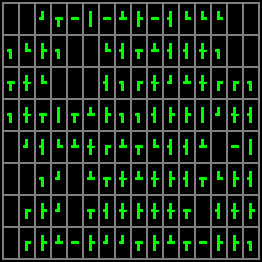
\includegraphics[scale=0.75]{\CURPATH/shuffled.png}
\caption{Разобранная головоломка}
\end{figure}

\dots и собранная:

\begin{figure}[H]
\label{fig:pipe_solved}
\centering
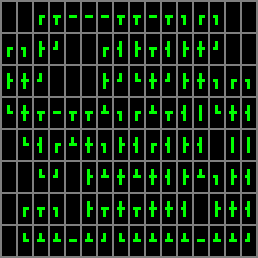
\includegraphics[scale=0.75]{\CURPATH/solved.png}
\caption{Собранная головоломка}
\end{figure}

Попробуем найти способ собрать её.

\subsubsection{Создание}

В начале, нужно её создать.
Вот простая идея.
Возьем массив ячеек 8*16.
Каждая ячейка может содержать какой-то тип блока.
Между ячейками есть стыки:

\pgfmathsetmacro\Width{16}
\pgfmathsetmacro\Height{8}
%\pgfmathsetmacro\Width{10}
%\pgfmathsetmacro\Height{5}
\pgfmathtruncatemacro\WidthMinusI{\Width - 1}
\pgfmathtruncatemacro\WidthMinusII{\Width - 2}
\pgfmathtruncatemacro\HeightMinusI{\Height - 1}
\pgfmathtruncatemacro\HeightMinusII{\Height - 2}
\pgfmathtruncatemacro\HeightPlusII{\Height + 2}
\pgfmathsetmacro\HeightPlusIi{\Height + 1.5}

% see also: http://www.texample.net/tikz/examples/euclid-algorithm/
\begin{center}
\begin{tikzpicture}[set style={{help lines}+=[dashed]},scale=0.7]

	\draw[style=help lines] (0,0) grid +(\Width,\Height);

	\foreach \c in {0,...,\WidthMinusI}
	{
		\foreach \r in {0,...,\HeightMinusII}
			\draw   [red,very thick,-] (\c+0.5,\r+0.75) -- (\c+0.5,\r+1.25);
		%\node[rotate=90] at (\c+0.5,\HeightPlusII) {\Large vjoints[\dots, \c] \normalsize};
		\node[rotate=90] at (\c+0.5,\HeightPlusII) {vjoints[\dots, \c]};
	}

	\foreach \r in {0,...,\HeightMinusI}
	{
		\foreach \c in {0,...,\WidthMinusII}
			\draw   [blue,very thick,-] (\c+0.75,\r+0.5) -- (\c+1.25,\r+0.5);
		\pgfmathtruncatemacro\hjointslabel{\HeightMinusI - \r}
		%\node at (-1.5,\r+0.5) {\large hjoints[\hjointslabel, \dots] \normalsize};
		\node at (-1.5,\r+0.5) {hjoints[\hjointslabel, \dots]};
	}

\end{tikzpicture}
\end{center}



Синие линии это горизонтальные стыки, красные линии это вертикальные стыки.
Мы просто случайно выставляем каждый стык в 0/false (отсутствует) или 1/true (присутствует).

После этого, теперь легко найти тип каждой ячейки.
А это:

\newcommand{\HeaderColor}{\cellcolor{blue!25}}
\begin{center}
\begin{longtable}{ | l | l | l | l | }
\hline
\HeaderColor стыки & \HeaderColor наше внутреннее название & \HeaderColor угол & \HeaderColor символ \\
\hline
0	&type 0		&	0$^{\circ}$	& (пробел)	\\
2	&type 2a	&	0$^{\circ}$	& \pmboxdrawuni{2503} \\ % ┃
2	&type 2a	&	90$^{\circ}$	& \pmboxdrawuni{2501} \\ % ━
2	&type 2b	&	0$^{\circ}$	& \pmboxdrawuni{250F} \\ % ┏
2	&type 2b	&	90$^{\circ}$	& \pmboxdrawuni{2513} \\ % ┓
2	&type 2b	&	180$^{\circ}$	& \pmboxdrawuni{251B} \\ % ┛
2	&type 2b	&	270$^{\circ}$	& \pmboxdrawuni{2517} \\ % ┗
3	&type 3		&	0$^{\circ}$	& \pmboxdrawuni{2523} \\ % ┣
3 	&type 3		&	90$^{\circ}$	& \pmboxdrawuni{2533} \\ % ┳
3	&type 3		&	180$^{\circ}$	& \pmboxdrawuni{252B} \\ % ┫
3	&type 3		&	270$^{\circ}$	& \pmboxdrawuni{253B} \\ % ┻
4	&type 4		&	0$^{\circ}$	& \pmboxdrawuni{254B} \\ % ╋
\hline
\end{longtable}
\end{center}

\textit{Висящие} стыки могут присутствовать на первой стадии (т.е., ячейки только с одним стыком), но они удалются
рекурсивно, и эти ячейки преобразуются в пустые ячейки.
Так что, в самом конце, все ячейки имеют минимум 2 стыка, и вся эта сантехническая система не имеет связей с внешним миром ---
я надеюсь, из-за этого станет немного проще.

Исходник генератора на Си здесь: \url{.../pipe/generator}.
Все вертикальные стыки хранятся в глобальном массиве \textit{hjoints[]} и вертикальные в \textit{vjoints[]}.

Программа на Си генерирует ANSI-раскрашенный вывод, как это было показано выше
(\ref{fig:pipe_shuffled}, \ref{fig:pipe_solved}) плюс массив типов для каждой ячейки, но без информации об углах:

\begin{lstlisting}[label=init_cells]
[
["0", "0", "2b", "3", "2a", "2a", "2a", "3", "3", "2a", "3", "2b", "2b", "2b", "0", "0"],
["2b", "2b", "3", "2b", "0", "0", "2b", "3", "3", "3", "3", "3", "4", "2b", "0", "0"],
["3", "4", "2b", "0", "0", "0", "3", "2b", "2b", "4", "2b", "3", "4", "2b", "2b", "2b"],
["2b", "4", "3", "2a", "3", "3", "3", "2b", "2b", "3", "3", "3", "2a", "2b", "4", "3"],
["0", "2b", "3", "2b", "3", "4", "2b", "3", "3", "2b", "3", "3", "3", "0", "2a", "2a"],
["0", "0", "2b", "2b", "0", "3", "3", "4", "3", "4", "3", "3", "3", "2b", "3", "3"],
["0", "2b", "3", "2b", "0", "3", "3", "4", "3", "4", "4", "3", "0", "3", "4", "3"],
["0", "2b", "3", "3", "2a", "3", "2b", "2b", "3", "3", "3", "3", "2a", "3", "3", "2b"],
]
\end{lstlisting}

\subsubsection{Решение}

Прежде всего, мы будем работать с массивом ячеек 8*16, где каждый элемент имеет 4 бита:
``T'' (top/верх),
``B'' (bottom/низ),
``L'' (left/лево),
``R'' (right/право).
Каждый бит представляет собой половину стыка.

% see also: http://www.texample.net/tikz/examples/euclid-algorithm/
\begin{center}
\begin{tikzpicture}[set style={{help lines}+=[dashed]},scale=0.7]

	\draw[style=help lines] (0,0) grid +(\Width,\Height);
	
	\foreach \c in {0,...,\WidthMinusI}
		%\node[rotate=90] at (\c+0.5,\HeightPlusIi) {\Large [\dots, \c] \normalsize};
		\node[rotate=90] at (\c+0.5,\HeightPlusIi) {[\dots, \c]};
	
	\foreach \r in {0,...,\HeightMinusI}
	{
		\pgfmathtruncatemacro\hlabel{\HeightMinusI - \r}
		%\node at (-1.5,\r+0.5) {\large [\hlabel, \dots] \normalsize};
		\node at (-1.5,\r+0.5) {[\hlabel, \dots]};
	
		\pgfmathsetmacro\Shift{0.325}
		\foreach \c in {0,...,\WidthMinusI}
		{
			\node at (\c+0.5,\r+0.5 + \Shift) {\footnotesize T \normalsize};
			\node at (\c+0.5,\r+0.5 - \Shift) {\footnotesize B \normalsize};
			\node at (\c+0.5 - \Shift,\r+0.5) {\footnotesize L \normalsize};
			\node at (\c+0.5 + \Shift,\r+0.5) {\footnotesize R \normalsize};
		}
	}

\end{tikzpicture}
\end{center}


Теперь определяем массив для каждого из четырех полустыков + информация об угле:

\begin{lstlisting}
HEIGHT=8
WIDTH=16

# if T/B/R/L is Bool instead of Int, Z3 solver will work faster
T=[[Bool('cell_%d_%d_top' % (r, c)) for c in range(WIDTH)] for r in range(HEIGHT)]
B=[[Bool('cell_%d_%d_bottom' % (r, c)) for c in range(WIDTH)] for r in range(HEIGHT)]
R=[[Bool('cell_%d_%d_right' % (r, c)) for c in range(WIDTH)] for r in range(HEIGHT)]
L=[[Bool('cell_%d_%d_left' % (r, c)) for c in range(WIDTH)] for r in range(HEIGHT)]
A=[[Int('cell_%d_%d_angle' % (r, c)) for c in range(WIDTH)] for r in range(HEIGHT)]
\end{lstlisting}

Мы знаем, что если каждый из полустыков присутствует, ответный полустык также должен присутствовать, и наоборот. 
Определяем всё это используя эти констрайнты:

\begin{lstlisting}
# shorthand variables for True and False:
t=True
f=False

# "top" of each cell must be equal to "bottom" of the cell above
# "bottom" of each cell must be equal to "top" of the cell below
# "left" of each cell must be equal to "right" of the cell at left
# "right" of each cell must be equal to "left" of the cell at right
for r in range(HEIGHT):
    for c in range(WIDTH):
        if r!=0:
            s.add(T[r][c]==B[r-1][c])
        if r!=HEIGHT-1:
            s.add(B[r][c]==T[r+1][c])
        if c!=0:
            s.add(L[r][c]==R[r][c-1])
        if c!=WIDTH-1:
            s.add(R[r][c]==L[r][c+1])

# "left" of each cell of first column shouldn't have any connection
# so is "right" of each cell of the last column
for r in range(HEIGHT):
    s.add(L[r][0]==f)
    s.add(R[r][WIDTH-1]==f)

# "top" of each cell of the first row shouldn't have any connection
# so is "bottom" of each cell of the last row
for c in range(WIDTH):
    s.add(T[0][c]==f)
    s.add(B[HEIGHT-1][c]==f)
\end{lstlisting}

Теперь перебираем все ячейки в изначальном массиве (\ref{init_cells}).
Первые две ячейки здесь пустые. И третья имеет тип ``2b''.
Это ``\pmboxdrawuni{250F}'' % ┏
и его можно ориентировать четырьмя разными способами.
И если её угол это 0$^{\circ}$, верхний и правый полустыки присутствуют, остальные отсутствуют.
Если он имеет угол 90$^{\circ}$, он выглядит как 
``\pmboxdrawuni{2513}'', % ┓
и верхник и левый полустыки присутствуют, остальные отсутствуют.

На обычном русском языке: ``если ячейка этого типа имеет угол 0$^{\circ}$, вот эти полустыки должны присутствовать \textbf{ИЛИ}
если она имеет угол 90$^{\circ}$, эти полустыки должны присутствовать, \textbf{ИЛИ}, итд, итд.''

Точно также, мы определяем эти правила для всех типов и всех возможных углов:

\begin{lstlisting}
for r in range(HEIGHT):
    for c in range(WIDTH):
        ty=cells_type[r][c]

        if ty=="0":
            s.add(A[r][c]==f)
            s.add(T[r][c]==f, B[r][c]==f, L[r][c]==f, R[r][c]==f)

        if ty=="2a":
            s.add(Or(And(A[r][c]==0, L[r][c]==f, R[r][c]==f, T[r][c]==t, B[r][c]==t),   # §\pmboxdrawuni{2503}§
                    And(A[r][c]==90, L[r][c]==t, R[r][c]==t, T[r][c]==f, B[r][c]==f)))  # §\pmboxdrawuni{2501}§

        if ty=="2b":
            s.add(Or(And(A[r][c]==0, L[r][c]==f, R[r][c]==t, T[r][c]==f, B[r][c]==t),   # §\pmboxdrawuni{250F}§
                    And(A[r][c]==90, L[r][c]==t, R[r][c]==f, T[r][c]==f, B[r][c]==t),   # §\pmboxdrawuni{2513}§
                    And(A[r][c]==180, L[r][c]==t, R[r][c]==f, T[r][c]==t, B[r][c]==f),  # §\pmboxdrawuni{251B}§
                    And(A[r][c]==270, L[r][c]==f, R[r][c]==t, T[r][c]==t, B[r][c]==f))) # §\pmboxdrawuni{2517}§
	
        if ty=="3":
            s.add(Or(And(A[r][c]==0, L[r][c]==f, R[r][c]==t, T[r][c]==t, B[r][c]==t),   # §\pmboxdrawuni{2523}§
                    And(A[r][c]==90, L[r][c]==t, R[r][c]==t, T[r][c]==f, B[r][c]==t),   # §\pmboxdrawuni{2533}§
                    And(A[r][c]==180, L[r][c]==t, R[r][c]==f, T[r][c]==t, B[r][c]==t),  # §\pmboxdrawuni{252B}§
                    And(A[r][c]==270, L[r][c]==t, R[r][c]==t, T[r][c]==t, B[r][c]==f))) # §\pmboxdrawuni{253B}§

        if ty=="4":
            s.add(A[r][c]==0)
            s.add(T[r][c]==t, B[r][c]==t, L[r][c]==t, R[r][c]==t) # §\pmboxdrawuni{254B}§
\end{lstlisting}

Полный исходник здесь: \url{.../solver/solve_pipe_puzzle1.py}.

Получается такой результат (выводит угол для каждой ячейки и (псевдо)графическое представление):

\begin{figure}[H]
\centering
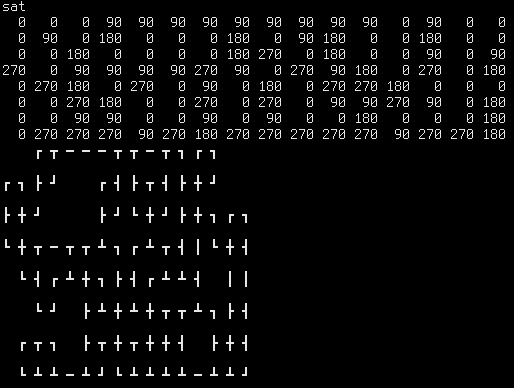
\includegraphics[scale=0.75]{\CURPATH/solver/solver.png}
\caption{Вывод скрипта солвера}
\end{figure}

Это работает $\approx 4$ секунды на моем старом и медленном Intel Atom N455 1.66GHz.
Быстро ли это? Не знаю, но снова вот что действительно круто, это то что мы понятия не имеем о какой-то математической
теории за всем этим, мы просто объявили ячейки, (полу-)стыки и определили отношения между ними.

Теперь следующий вопрос это, сколько здесь возможных решений?
Используя раннее описанный метод (\ref{SMTEnumerate}), я немного изменил скрипт солвера
\footnote{\url{.../solver/solve_pipe_puzzle2.py}} и солвер
сказал что возможно два решения.

Сравним их используя gvimdiff:

\begin{figure}[H]
\centering
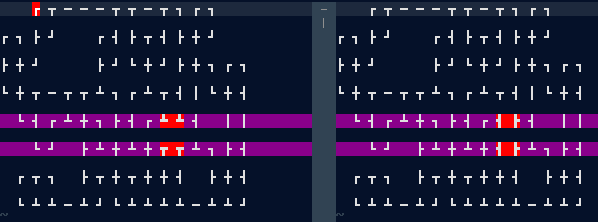
\includegraphics[scale=0.75]{\CURPATH/solver/diff.png}
\caption{Вывод gvimdiff (извините за мой красный курсор в левой части в левом верхнем углу)}
\end{figure}

4 ячейки в середине могут быть ориентированы по-разному.
Видимо, другие головоломки могут также выдавать разные результаты.

P.S.
\textit{Полу-стык} определен как булевый тип.
Но на самом деле, первая версия солвера была написана используя целочисленный тип для полу-стыков,
и 0 использовалось для False и 1 для True.
Я так сделал, потому что хотел более компактный исходный код, без использования длинных слов как ``False'' и ``True''.
И это работало, но медленнее. Вероятно, Z3 работает с булевыми типами быстрее? Лучше?
Так или иначе, я пишу это чтобы отметить, что, если нужно, целочисленный тип можно использовать вместо булевого.


\section{Развлекательная математика и головоломки}

\subsection{Судоку}

Головоломка Судоку это решетка 9*9, некоторые ячейки заполнены значениями, некоторые пустые:

% copypasted from http://www.texample.net/tikz/examples/sudoku/
\newcounter{row}
\newcounter{col}

\newcommand\setrow[9]{
  \setcounter{col}{1}
  \foreach \n in {#1, #2, #3, #4, #5, #6, #7, #8, #9} {
    \edef\x{\value{col} - 0.5}
    \edef\y{9.5 - \value{row}}
    \node[anchor=center] at (\x, \y) {\n};
    \stepcounter{col}
  }
  \stepcounter{row}
}

\begin{center}
\begin{tikzpicture}[scale=.7]
  \begin{scope}
    \draw (0, 0) grid (9, 9);
    \draw[very thick, scale=3] (0, 0) grid (3, 3);

    \setcounter{row}{1}
    \setrow { }{ }{5}  {3}{ }{ }  { }{ }{ }
    \setrow {8}{ }{ }  { }{ }{ }  { }{2}{ }
    \setrow { }{7}{ }  { }{1}{ }  {5}{ }{ }

    \setrow {4}{ }{ }  { }{ }{5}  {3}{ }{ }
    \setrow { }{1}{ }  { }{7}{ }  { }{ }{6}
    \setrow { }{ }{3}  {2}{ }{ }  { }{8}{ }

    \setrow { }{6}{ }  {5}{ }{ }  { }{ }{9}
    \setrow { }{ }{4}  { }{ }{ }  { }{3}{ }
    \setrow { }{ }{ }  { }{ }{9}  {7}{ }{ }

    \node[anchor=center] at (4.5, -0.5) {Нерешенная Судоку};
  \end{scope}
\end{tikzpicture}
\end{center}

Числа в каждом ряду должны быть уникальными, т.е., каждый ряд должен содержать 9 чисел в пределах 1..9 без повторений.
Та же история и для каждого столбца и каждого квадрата 3*3.

Головоломка представляет собой хороший кандидат, на котором можно попробовать \ac{SMT}-солвер, потому что это,
в общем-то, просто нерешенная система уравнений.

\input{puzzles/sudoku/1/main_RU}
%\input{puzzles/sudoku/GT/main_RU}
%\input{puzzles/sudoku/killer/main_RU}
\input{puzzles/sudoku/KLEE/main_RU}
\input{puzzles/sudoku/SAT/main_RU}


\subsection{Головоломка зебры (\ac{AKA} Загадка Эйнштейна)}

\input{puzzles/zebra/SMT/main_RU}
\input{puzzles/zebra/KLEE/main_RU}
\input{puzzles/zebra/SAT/main_RU}


\subsection{Решение головоломки ``трубы'' используя Z3 SMT-солвер}

\renewcommand{\CURPATH}{puzzles/pipe}

Головоломка ``трубы'' это популярная головоломка (просто погуглите ``pipe puzzle'' и посмотрите на картинки).

Вот как выглядит головоломка в разобранном виде:

\begin{figure}[H]
\label{fig:pipe_shuffled}
\centering
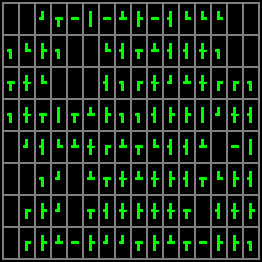
\includegraphics[scale=0.75]{\CURPATH/shuffled.png}
\caption{Разобранная головоломка}
\end{figure}

\dots и собранная:

\begin{figure}[H]
\label{fig:pipe_solved}
\centering
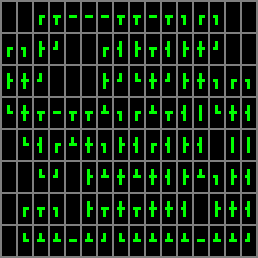
\includegraphics[scale=0.75]{\CURPATH/solved.png}
\caption{Собранная головоломка}
\end{figure}

Попробуем найти способ собрать её.

\subsubsection{Создание}

В начале, нужно её создать.
Вот простая идея.
Возьем массив ячеек 8*16.
Каждая ячейка может содержать какой-то тип блока.
Между ячейками есть стыки:

\input{\CURPATH/pipe_gen.tex}

Синие линии это горизонтальные стыки, красные линии это вертикальные стыки.
Мы просто случайно выставляем каждый стык в 0/false (отсутствует) или 1/true (присутствует).

После этого, теперь легко найти тип каждой ячейки.
А это:

\newcommand{\HeaderColor}{\cellcolor{blue!25}}
\begin{center}
\begin{longtable}{ | l | l | l | l | }
\hline
\HeaderColor стыки & \HeaderColor наше внутреннее название & \HeaderColor угол & \HeaderColor символ \\
\hline
0	&type 0		&	0$^{\circ}$	& (пробел)	\\
2	&type 2a	&	0$^{\circ}$	& \pmboxdrawuni{2503} \\ % ┃
2	&type 2a	&	90$^{\circ}$	& \pmboxdrawuni{2501} \\ % ━
2	&type 2b	&	0$^{\circ}$	& \pmboxdrawuni{250F} \\ % ┏
2	&type 2b	&	90$^{\circ}$	& \pmboxdrawuni{2513} \\ % ┓
2	&type 2b	&	180$^{\circ}$	& \pmboxdrawuni{251B} \\ % ┛
2	&type 2b	&	270$^{\circ}$	& \pmboxdrawuni{2517} \\ % ┗
3	&type 3		&	0$^{\circ}$	& \pmboxdrawuni{2523} \\ % ┣
3 	&type 3		&	90$^{\circ}$	& \pmboxdrawuni{2533} \\ % ┳
3	&type 3		&	180$^{\circ}$	& \pmboxdrawuni{252B} \\ % ┫
3	&type 3		&	270$^{\circ}$	& \pmboxdrawuni{253B} \\ % ┻
4	&type 4		&	0$^{\circ}$	& \pmboxdrawuni{254B} \\ % ╋
\hline
\end{longtable}
\end{center}

\textit{Висящие} стыки могут присутствовать на первой стадии (т.е., ячейки только с одним стыком), но они удалются
рекурсивно, и эти ячейки преобразуются в пустые ячейки.
Так что, в самом конце, все ячейки имеют минимум 2 стыка, и вся эта сантехническая система не имеет связей с внешним миром ---
я надеюсь, из-за этого станет немного проще.

Исходник генератора на Си здесь: \url{.../pipe/generator}.
Все вертикальные стыки хранятся в глобальном массиве \textit{hjoints[]} и вертикальные в \textit{vjoints[]}.

Программа на Си генерирует ANSI-раскрашенный вывод, как это было показано выше
(\ref{fig:pipe_shuffled}, \ref{fig:pipe_solved}) плюс массив типов для каждой ячейки, но без информации об углах:

\begin{lstlisting}[label=init_cells]
[
["0", "0", "2b", "3", "2a", "2a", "2a", "3", "3", "2a", "3", "2b", "2b", "2b", "0", "0"],
["2b", "2b", "3", "2b", "0", "0", "2b", "3", "3", "3", "3", "3", "4", "2b", "0", "0"],
["3", "4", "2b", "0", "0", "0", "3", "2b", "2b", "4", "2b", "3", "4", "2b", "2b", "2b"],
["2b", "4", "3", "2a", "3", "3", "3", "2b", "2b", "3", "3", "3", "2a", "2b", "4", "3"],
["0", "2b", "3", "2b", "3", "4", "2b", "3", "3", "2b", "3", "3", "3", "0", "2a", "2a"],
["0", "0", "2b", "2b", "0", "3", "3", "4", "3", "4", "3", "3", "3", "2b", "3", "3"],
["0", "2b", "3", "2b", "0", "3", "3", "4", "3", "4", "4", "3", "0", "3", "4", "3"],
["0", "2b", "3", "3", "2a", "3", "2b", "2b", "3", "3", "3", "3", "2a", "3", "3", "2b"],
]
\end{lstlisting}

\subsubsection{Решение}

Прежде всего, мы будем работать с массивом ячеек 8*16, где каждый элемент имеет 4 бита:
``T'' (top/верх),
``B'' (bottom/низ),
``L'' (left/лево),
``R'' (right/право).
Каждый бит представляет собой половину стыка.

\input{\CURPATH/pipe_solve.tex}

Теперь определяем массив для каждого из четырех полустыков + информация об угле:

\begin{lstlisting}
HEIGHT=8
WIDTH=16

# if T/B/R/L is Bool instead of Int, Z3 solver will work faster
T=[[Bool('cell_%d_%d_top' % (r, c)) for c in range(WIDTH)] for r in range(HEIGHT)]
B=[[Bool('cell_%d_%d_bottom' % (r, c)) for c in range(WIDTH)] for r in range(HEIGHT)]
R=[[Bool('cell_%d_%d_right' % (r, c)) for c in range(WIDTH)] for r in range(HEIGHT)]
L=[[Bool('cell_%d_%d_left' % (r, c)) for c in range(WIDTH)] for r in range(HEIGHT)]
A=[[Int('cell_%d_%d_angle' % (r, c)) for c in range(WIDTH)] for r in range(HEIGHT)]
\end{lstlisting}

Мы знаем, что если каждый из полустыков присутствует, ответный полустык также должен присутствовать, и наоборот. 
Определяем всё это используя эти констрайнты:

\begin{lstlisting}
# shorthand variables for True and False:
t=True
f=False

# "top" of each cell must be equal to "bottom" of the cell above
# "bottom" of each cell must be equal to "top" of the cell below
# "left" of each cell must be equal to "right" of the cell at left
# "right" of each cell must be equal to "left" of the cell at right
for r in range(HEIGHT):
    for c in range(WIDTH):
        if r!=0:
            s.add(T[r][c]==B[r-1][c])
        if r!=HEIGHT-1:
            s.add(B[r][c]==T[r+1][c])
        if c!=0:
            s.add(L[r][c]==R[r][c-1])
        if c!=WIDTH-1:
            s.add(R[r][c]==L[r][c+1])

# "left" of each cell of first column shouldn't have any connection
# so is "right" of each cell of the last column
for r in range(HEIGHT):
    s.add(L[r][0]==f)
    s.add(R[r][WIDTH-1]==f)

# "top" of each cell of the first row shouldn't have any connection
# so is "bottom" of each cell of the last row
for c in range(WIDTH):
    s.add(T[0][c]==f)
    s.add(B[HEIGHT-1][c]==f)
\end{lstlisting}

Теперь перебираем все ячейки в изначальном массиве (\ref{init_cells}).
Первые две ячейки здесь пустые. И третья имеет тип ``2b''.
Это ``\pmboxdrawuni{250F}'' % ┏
и его можно ориентировать четырьмя разными способами.
И если её угол это 0$^{\circ}$, верхний и правый полустыки присутствуют, остальные отсутствуют.
Если он имеет угол 90$^{\circ}$, он выглядит как 
``\pmboxdrawuni{2513}'', % ┓
и верхник и левый полустыки присутствуют, остальные отсутствуют.

На обычном русском языке: ``если ячейка этого типа имеет угол 0$^{\circ}$, вот эти полустыки должны присутствовать \textbf{ИЛИ}
если она имеет угол 90$^{\circ}$, эти полустыки должны присутствовать, \textbf{ИЛИ}, итд, итд.''

Точно также, мы определяем эти правила для всех типов и всех возможных углов:

\begin{lstlisting}
for r in range(HEIGHT):
    for c in range(WIDTH):
        ty=cells_type[r][c]

        if ty=="0":
            s.add(A[r][c]==f)
            s.add(T[r][c]==f, B[r][c]==f, L[r][c]==f, R[r][c]==f)

        if ty=="2a":
            s.add(Or(And(A[r][c]==0, L[r][c]==f, R[r][c]==f, T[r][c]==t, B[r][c]==t),   # §\pmboxdrawuni{2503}§
                    And(A[r][c]==90, L[r][c]==t, R[r][c]==t, T[r][c]==f, B[r][c]==f)))  # §\pmboxdrawuni{2501}§

        if ty=="2b":
            s.add(Or(And(A[r][c]==0, L[r][c]==f, R[r][c]==t, T[r][c]==f, B[r][c]==t),   # §\pmboxdrawuni{250F}§
                    And(A[r][c]==90, L[r][c]==t, R[r][c]==f, T[r][c]==f, B[r][c]==t),   # §\pmboxdrawuni{2513}§
                    And(A[r][c]==180, L[r][c]==t, R[r][c]==f, T[r][c]==t, B[r][c]==f),  # §\pmboxdrawuni{251B}§
                    And(A[r][c]==270, L[r][c]==f, R[r][c]==t, T[r][c]==t, B[r][c]==f))) # §\pmboxdrawuni{2517}§
	
        if ty=="3":
            s.add(Or(And(A[r][c]==0, L[r][c]==f, R[r][c]==t, T[r][c]==t, B[r][c]==t),   # §\pmboxdrawuni{2523}§
                    And(A[r][c]==90, L[r][c]==t, R[r][c]==t, T[r][c]==f, B[r][c]==t),   # §\pmboxdrawuni{2533}§
                    And(A[r][c]==180, L[r][c]==t, R[r][c]==f, T[r][c]==t, B[r][c]==t),  # §\pmboxdrawuni{252B}§
                    And(A[r][c]==270, L[r][c]==t, R[r][c]==t, T[r][c]==t, B[r][c]==f))) # §\pmboxdrawuni{253B}§

        if ty=="4":
            s.add(A[r][c]==0)
            s.add(T[r][c]==t, B[r][c]==t, L[r][c]==t, R[r][c]==t) # §\pmboxdrawuni{254B}§
\end{lstlisting}

Полный исходник здесь: \url{.../solver/solve_pipe_puzzle1.py}.

Получается такой результат (выводит угол для каждой ячейки и (псевдо)графическое представление):

\begin{figure}[H]
\centering
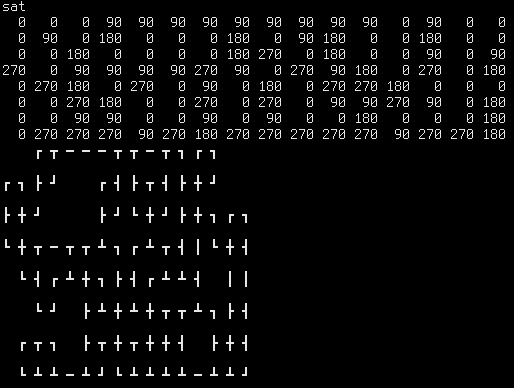
\includegraphics[scale=0.75]{\CURPATH/solver/solver.png}
\caption{Вывод скрипта солвера}
\end{figure}

Это работает $\approx 4$ секунды на моем старом и медленном Intel Atom N455 1.66GHz.
Быстро ли это? Не знаю, но снова вот что действительно круто, это то что мы понятия не имеем о какой-то математической
теории за всем этим, мы просто объявили ячейки, (полу-)стыки и определили отношения между ними.

Теперь следующий вопрос это, сколько здесь возможных решений?
Используя раннее описанный метод (\ref{SMTEnumerate}), я немного изменил скрипт солвера
\footnote{\url{.../solver/solve_pipe_puzzle2.py}} и солвер
сказал что возможно два решения.

Сравним их используя gvimdiff:

\begin{figure}[H]
\centering
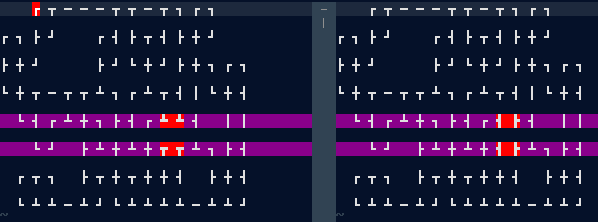
\includegraphics[scale=0.75]{\CURPATH/solver/diff.png}
\caption{Вывод gvimdiff (извините за мой красный курсор в левой части в левом верхнем углу)}
\end{figure}

4 ячейки в середине могут быть ориентированы по-разному.
Видимо, другие головоломки могут также выдавать разные результаты.

P.S.
\textit{Полу-стык} определен как булевый тип.
Но на самом деле, первая версия солвера была написана используя целочисленный тип для полу-стыков,
и 0 использовалось для False и 1 для True.
Я так сделал, потому что хотел более компактный исходный код, без использования длинных слов как ``False'' и ``True''.
И это работало, но медленнее. Вероятно, Z3 работает с булевыми типами быстрее? Лучше?
Так или иначе, я пишу это чтобы отметить, что, если нужно, целочисленный тип можно использовать вместо булевого.


\section{Развлекательная математика и головоломки}

\input{puzzles/sudoku/main_RU}
\input{puzzles/zebra/main_RU}
\input{puzzles/pipe/main_RU}
\input{puzzles/rubik2/failed_SMT/main_RU}
\input{puzzles/rubik2/SAT/main_RU}
\input{puzzles/rubik3/one_face_SMT/main_RU}
%\input{puzzles/numberlink/main_RU}
%\input{puzzles/two_parks_RU}
\input{puzzles/alphametics/main_RU}
%\input{puzzles/2015_AIME_II_Problems_12_RU}
%\input{puzzles/fred/main_RU}
%\input{puzzles/MC/main_RU}
%\input{puzzles/coin_flip/main_RU}
%\input{puzzles/Mock_AIME_2_2006-2007_Problem_8_RU}
%\input{puzzles/2012_AIME_I_Problems_1_RU}
%\input{puzzles/keypad_RU}


\section{Развлекательная математика и головоломки}

\input{puzzles/sudoku/main_RU}
\input{puzzles/zebra/main_RU}
\input{puzzles/pipe/main_RU}
\input{puzzles/rubik2/failed_SMT/main_RU}
\input{puzzles/rubik2/SAT/main_RU}
\input{puzzles/rubik3/one_face_SMT/main_RU}
%\input{puzzles/numberlink/main_RU}
%\input{puzzles/two_parks_RU}
\input{puzzles/alphametics/main_RU}
%\input{puzzles/2015_AIME_II_Problems_12_RU}
%\input{puzzles/fred/main_RU}
%\input{puzzles/MC/main_RU}
%\input{puzzles/coin_flip/main_RU}
%\input{puzzles/Mock_AIME_2_2006-2007_Problem_8_RU}
%\input{puzzles/2012_AIME_I_Problems_1_RU}
%\input{puzzles/keypad_RU}


\section{Развлекательная математика и головоломки}

\input{puzzles/sudoku/main_RU}
\input{puzzles/zebra/main_RU}
\input{puzzles/pipe/main_RU}
\input{puzzles/rubik2/failed_SMT/main_RU}
\input{puzzles/rubik2/SAT/main_RU}
\input{puzzles/rubik3/one_face_SMT/main_RU}
%\input{puzzles/numberlink/main_RU}
%\input{puzzles/two_parks_RU}
\input{puzzles/alphametics/main_RU}
%\input{puzzles/2015_AIME_II_Problems_12_RU}
%\input{puzzles/fred/main_RU}
%\input{puzzles/MC/main_RU}
%\input{puzzles/coin_flip/main_RU}
%\input{puzzles/Mock_AIME_2_2006-2007_Problem_8_RU}
%\input{puzzles/2012_AIME_I_Problems_1_RU}
%\input{puzzles/keypad_RU}


%\section{Развлекательная математика и головоломки}

\input{puzzles/sudoku/main_RU}
\input{puzzles/zebra/main_RU}
\input{puzzles/pipe/main_RU}
\input{puzzles/rubik2/failed_SMT/main_RU}
\input{puzzles/rubik2/SAT/main_RU}
\input{puzzles/rubik3/one_face_SMT/main_RU}
%\input{puzzles/numberlink/main_RU}
%\input{puzzles/two_parks_RU}
\input{puzzles/alphametics/main_RU}
%\input{puzzles/2015_AIME_II_Problems_12_RU}
%\input{puzzles/fred/main_RU}
%\input{puzzles/MC/main_RU}
%\input{puzzles/coin_flip/main_RU}
%\input{puzzles/Mock_AIME_2_2006-2007_Problem_8_RU}
%\input{puzzles/2012_AIME_I_Problems_1_RU}
%\input{puzzles/keypad_RU}


%\input{puzzles/two_parks_RU}
\subsection{Альфаметика}

Согласно Дональду Кнуту, термин ``Альфаметика'' был придуман Дж. Эйч. Аш. Хантером.
Это головоломка: какие десятичные цифры в пределах 0..9 нужно присвоить каждой букве, чтобы это уравнение было справедливо?

\begin{lstlisting}
  SEND
+ MORE
 -----
 MONEY
\end{lstlisting}

Для Z3 это легко:

\lstinputlisting{puzzles/alphametics/alpha.py}

Вывод:

\begin{lstlisting}
sat
[E, = 5,
 S, = 9,
 M, = 1,
 N, = 6,
 D, = 7,
 R, = 8,
 O, = 0,
 Y = 2]
\end{lstlisting}

Вот еще одна, из \ac{TAOCP} том IV (\url{http://www-cs-faculty.stanford.edu/~uno/fasc2b.ps.gz}):

\lstinputlisting{puzzles/alphametics/alpha2.py}

\begin{lstlisting}
sat
[L, = 6,
 S, = 7,
 N, = 2,
 T, = 1,
 I, = 5,
 V = 3,
 A, = 8,
 R, = 9,
 O, = 4,
 TRIO = 1954,
 SONATA, = 742818,
 VIOLA, = 35468,
 VIOLIN, = 354652]
\end{lstlisting}

% TODO URL
Эту головоломку я нашел в примерах pySMT:

\lstinputlisting{puzzles/alphametics/alpha3.py}

\begin{lstlisting}
sat
[D = 5, R = 4, O = 3, E = 8, L = 6, W = 7, H = 2]
\end{lstlisting}

%%% 

Это упражнение Q209 из
[Companion to the Papers of Donald Knuth]\footnote{\url{http://www-cs-faculty.stanford.edu/~knuth/cp.html}}.

\begin{lstlisting}
 KNIFE
  FORK
 SPOON
  SOUP
------
SUPPER
\end{lstlisting}

В целях упрощения, я добавил ф-цию (list\_to\_expr()):

\lstinputlisting{puzzles/alphametics/alpha4.py}

\begin{lstlisting}
sat
[K = 7,
 N = 4,
 R = 9,
 I = 1,
 E = 6,
 S = 0,
 O = 3,
 F = 5,
 U = 8,
 P = 2,
 SUPPER = 82269,
 SOUP = 382,
 SPOON = 2334,
 FORK = 5397,
 KNIFE = 74156]
\end{lstlisting}

S это 0, так что значение SUPPER начинается с (убранного) нуля. Скажем так, нам это не нравится.
Добавим это, чтобы это исправить:

\begin{lstlisting}
s.add(S!=0)
\end{lstlisting}

\begin{lstlisting}
sat
[K = 8,
 N = 4,
 R = 3,
 I = 7,
 E = 6,
 S = 1,
 O = 9,
 F = 2,
 U = 0,
 P = 5,
 SUPPER = 105563,
 SOUP = 1905,
 SPOON = 15994,
 FORK = 2938,
 KNIFE = 84726]
\end{lstlisting}

\paragraph{Создание своей собственной головоломки}

Вот проблема: есть только 10 букв, но как их выбрать из числа слов?
Мы можем использовать Z3 для этого:

\lstinputlisting{puzzles/alphametics/gen.py}

Это первая сгенерированная головоломка:

\begin{lstlisting}
sat
EGGS
JELLY
LUNCH
C 5
E 6
G 3
H 7
J 0
L 1
N 4
S 8
U 2
Y 9
\end{lstlisting}

Что если мы хотим, чтобы слово ``CAKE'' присутствовало в числе ``слагаемых''?

Добавим это:

\begin{lstlisting}
s.add(word_used[words.index('CAKE')])
\end{lstlisting}

\begin{lstlisting}
sat
CAKE
TEA
LUNCH
A 8
C 3
E 1
H 9
J 6
K 2
L 0
N 5
T 7
U 4
\end{lstlisting}

Добавим это:

\begin{lstlisting}
s.add(word_used[words.index('EGGS')])
\end{lstlisting}

Теперь оно может найти пару к EGGS:

\begin{lstlisting}
sat
EGGS
HONEY
LUNCH
C 6
E 7
G 9
H 4
L 5
N 8
O 2
S 3
U 0
Y 1
\end{lstlisting}

\paragraph{Файлы}

\url{https://github.com/DennisYurichev/...}




%\input{puzzles/2015_AIME_II_Problems_12_RU}
%\section{Развлекательная математика и головоломки}

\input{puzzles/sudoku/main_RU}
\input{puzzles/zebra/main_RU}
\input{puzzles/pipe/main_RU}
\input{puzzles/rubik2/failed_SMT/main_RU}
\input{puzzles/rubik2/SAT/main_RU}
\input{puzzles/rubik3/one_face_SMT/main_RU}
%\input{puzzles/numberlink/main_RU}
%\input{puzzles/two_parks_RU}
\input{puzzles/alphametics/main_RU}
%\input{puzzles/2015_AIME_II_Problems_12_RU}
%\input{puzzles/fred/main_RU}
%\input{puzzles/MC/main_RU}
%\input{puzzles/coin_flip/main_RU}
%\input{puzzles/Mock_AIME_2_2006-2007_Problem_8_RU}
%\input{puzzles/2012_AIME_I_Problems_1_RU}
%\input{puzzles/keypad_RU}


%\section{Развлекательная математика и головоломки}

\input{puzzles/sudoku/main_RU}
\input{puzzles/zebra/main_RU}
\input{puzzles/pipe/main_RU}
\input{puzzles/rubik2/failed_SMT/main_RU}
\input{puzzles/rubik2/SAT/main_RU}
\input{puzzles/rubik3/one_face_SMT/main_RU}
%\input{puzzles/numberlink/main_RU}
%\input{puzzles/two_parks_RU}
\input{puzzles/alphametics/main_RU}
%\input{puzzles/2015_AIME_II_Problems_12_RU}
%\input{puzzles/fred/main_RU}
%\input{puzzles/MC/main_RU}
%\input{puzzles/coin_flip/main_RU}
%\input{puzzles/Mock_AIME_2_2006-2007_Problem_8_RU}
%\input{puzzles/2012_AIME_I_Problems_1_RU}
%\input{puzzles/keypad_RU}


%\section{Развлекательная математика и головоломки}

\input{puzzles/sudoku/main_RU}
\input{puzzles/zebra/main_RU}
\input{puzzles/pipe/main_RU}
\input{puzzles/rubik2/failed_SMT/main_RU}
\input{puzzles/rubik2/SAT/main_RU}
\input{puzzles/rubik3/one_face_SMT/main_RU}
%\input{puzzles/numberlink/main_RU}
%\input{puzzles/two_parks_RU}
\input{puzzles/alphametics/main_RU}
%\input{puzzles/2015_AIME_II_Problems_12_RU}
%\input{puzzles/fred/main_RU}
%\input{puzzles/MC/main_RU}
%\input{puzzles/coin_flip/main_RU}
%\input{puzzles/Mock_AIME_2_2006-2007_Problem_8_RU}
%\input{puzzles/2012_AIME_I_Problems_1_RU}
%\input{puzzles/keypad_RU}


%\input{puzzles/Mock_AIME_2_2006-2007_Problem_8_RU}
%\input{puzzles/2012_AIME_I_Problems_1_RU}
%\input{puzzles/keypad_RU}


\section{Развлекательная математика и головоломки}

\subsection{Судоку}

Головоломка Судоку это решетка 9*9, некоторые ячейки заполнены значениями, некоторые пустые:

% copypasted from http://www.texample.net/tikz/examples/sudoku/
\newcounter{row}
\newcounter{col}

\newcommand\setrow[9]{
  \setcounter{col}{1}
  \foreach \n in {#1, #2, #3, #4, #5, #6, #7, #8, #9} {
    \edef\x{\value{col} - 0.5}
    \edef\y{9.5 - \value{row}}
    \node[anchor=center] at (\x, \y) {\n};
    \stepcounter{col}
  }
  \stepcounter{row}
}

\begin{center}
\begin{tikzpicture}[scale=.7]
  \begin{scope}
    \draw (0, 0) grid (9, 9);
    \draw[very thick, scale=3] (0, 0) grid (3, 3);

    \setcounter{row}{1}
    \setrow { }{ }{5}  {3}{ }{ }  { }{ }{ }
    \setrow {8}{ }{ }  { }{ }{ }  { }{2}{ }
    \setrow { }{7}{ }  { }{1}{ }  {5}{ }{ }

    \setrow {4}{ }{ }  { }{ }{5}  {3}{ }{ }
    \setrow { }{1}{ }  { }{7}{ }  { }{ }{6}
    \setrow { }{ }{3}  {2}{ }{ }  { }{8}{ }

    \setrow { }{6}{ }  {5}{ }{ }  { }{ }{9}
    \setrow { }{ }{4}  { }{ }{ }  { }{3}{ }
    \setrow { }{ }{ }  { }{ }{9}  {7}{ }{ }

    \node[anchor=center] at (4.5, -0.5) {Нерешенная Судоку};
  \end{scope}
\end{tikzpicture}
\end{center}

Числа в каждом ряду должны быть уникальными, т.е., каждый ряд должен содержать 9 чисел в пределах 1..9 без повторений.
Та же история и для каждого столбца и каждого квадрата 3*3.

Головоломка представляет собой хороший кандидат, на котором можно попробовать \ac{SMT}-солвер, потому что это,
в общем-то, просто нерешенная система уравнений.

\input{puzzles/sudoku/1/main_RU}
%\input{puzzles/sudoku/GT/main_RU}
%\input{puzzles/sudoku/killer/main_RU}
\input{puzzles/sudoku/KLEE/main_RU}
\input{puzzles/sudoku/SAT/main_RU}


\subsection{Головоломка зебры (\ac{AKA} Загадка Эйнштейна)}

\input{puzzles/zebra/SMT/main_RU}
\input{puzzles/zebra/KLEE/main_RU}
\input{puzzles/zebra/SAT/main_RU}


\subsection{Решение головоломки ``трубы'' используя Z3 SMT-солвер}

\renewcommand{\CURPATH}{puzzles/pipe}

Головоломка ``трубы'' это популярная головоломка (просто погуглите ``pipe puzzle'' и посмотрите на картинки).

Вот как выглядит головоломка в разобранном виде:

\begin{figure}[H]
\label{fig:pipe_shuffled}
\centering
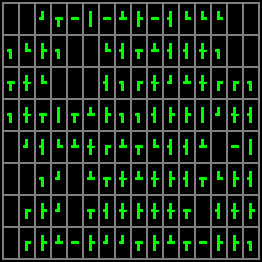
\includegraphics[scale=0.75]{\CURPATH/shuffled.png}
\caption{Разобранная головоломка}
\end{figure}

\dots и собранная:

\begin{figure}[H]
\label{fig:pipe_solved}
\centering
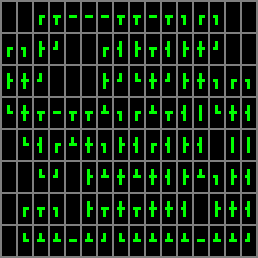
\includegraphics[scale=0.75]{\CURPATH/solved.png}
\caption{Собранная головоломка}
\end{figure}

Попробуем найти способ собрать её.

\subsubsection{Создание}

В начале, нужно её создать.
Вот простая идея.
Возьем массив ячеек 8*16.
Каждая ячейка может содержать какой-то тип блока.
Между ячейками есть стыки:

\input{\CURPATH/pipe_gen.tex}

Синие линии это горизонтальные стыки, красные линии это вертикальные стыки.
Мы просто случайно выставляем каждый стык в 0/false (отсутствует) или 1/true (присутствует).

После этого, теперь легко найти тип каждой ячейки.
А это:

\newcommand{\HeaderColor}{\cellcolor{blue!25}}
\begin{center}
\begin{longtable}{ | l | l | l | l | }
\hline
\HeaderColor стыки & \HeaderColor наше внутреннее название & \HeaderColor угол & \HeaderColor символ \\
\hline
0	&type 0		&	0$^{\circ}$	& (пробел)	\\
2	&type 2a	&	0$^{\circ}$	& \pmboxdrawuni{2503} \\ % ┃
2	&type 2a	&	90$^{\circ}$	& \pmboxdrawuni{2501} \\ % ━
2	&type 2b	&	0$^{\circ}$	& \pmboxdrawuni{250F} \\ % ┏
2	&type 2b	&	90$^{\circ}$	& \pmboxdrawuni{2513} \\ % ┓
2	&type 2b	&	180$^{\circ}$	& \pmboxdrawuni{251B} \\ % ┛
2	&type 2b	&	270$^{\circ}$	& \pmboxdrawuni{2517} \\ % ┗
3	&type 3		&	0$^{\circ}$	& \pmboxdrawuni{2523} \\ % ┣
3 	&type 3		&	90$^{\circ}$	& \pmboxdrawuni{2533} \\ % ┳
3	&type 3		&	180$^{\circ}$	& \pmboxdrawuni{252B} \\ % ┫
3	&type 3		&	270$^{\circ}$	& \pmboxdrawuni{253B} \\ % ┻
4	&type 4		&	0$^{\circ}$	& \pmboxdrawuni{254B} \\ % ╋
\hline
\end{longtable}
\end{center}

\textit{Висящие} стыки могут присутствовать на первой стадии (т.е., ячейки только с одним стыком), но они удалются
рекурсивно, и эти ячейки преобразуются в пустые ячейки.
Так что, в самом конце, все ячейки имеют минимум 2 стыка, и вся эта сантехническая система не имеет связей с внешним миром ---
я надеюсь, из-за этого станет немного проще.

Исходник генератора на Си здесь: \url{.../pipe/generator}.
Все вертикальные стыки хранятся в глобальном массиве \textit{hjoints[]} и вертикальные в \textit{vjoints[]}.

Программа на Си генерирует ANSI-раскрашенный вывод, как это было показано выше
(\ref{fig:pipe_shuffled}, \ref{fig:pipe_solved}) плюс массив типов для каждой ячейки, но без информации об углах:

\begin{lstlisting}[label=init_cells]
[
["0", "0", "2b", "3", "2a", "2a", "2a", "3", "3", "2a", "3", "2b", "2b", "2b", "0", "0"],
["2b", "2b", "3", "2b", "0", "0", "2b", "3", "3", "3", "3", "3", "4", "2b", "0", "0"],
["3", "4", "2b", "0", "0", "0", "3", "2b", "2b", "4", "2b", "3", "4", "2b", "2b", "2b"],
["2b", "4", "3", "2a", "3", "3", "3", "2b", "2b", "3", "3", "3", "2a", "2b", "4", "3"],
["0", "2b", "3", "2b", "3", "4", "2b", "3", "3", "2b", "3", "3", "3", "0", "2a", "2a"],
["0", "0", "2b", "2b", "0", "3", "3", "4", "3", "4", "3", "3", "3", "2b", "3", "3"],
["0", "2b", "3", "2b", "0", "3", "3", "4", "3", "4", "4", "3", "0", "3", "4", "3"],
["0", "2b", "3", "3", "2a", "3", "2b", "2b", "3", "3", "3", "3", "2a", "3", "3", "2b"],
]
\end{lstlisting}

\subsubsection{Решение}

Прежде всего, мы будем работать с массивом ячеек 8*16, где каждый элемент имеет 4 бита:
``T'' (top/верх),
``B'' (bottom/низ),
``L'' (left/лево),
``R'' (right/право).
Каждый бит представляет собой половину стыка.

\input{\CURPATH/pipe_solve.tex}

Теперь определяем массив для каждого из четырех полустыков + информация об угле:

\begin{lstlisting}
HEIGHT=8
WIDTH=16

# if T/B/R/L is Bool instead of Int, Z3 solver will work faster
T=[[Bool('cell_%d_%d_top' % (r, c)) for c in range(WIDTH)] for r in range(HEIGHT)]
B=[[Bool('cell_%d_%d_bottom' % (r, c)) for c in range(WIDTH)] for r in range(HEIGHT)]
R=[[Bool('cell_%d_%d_right' % (r, c)) for c in range(WIDTH)] for r in range(HEIGHT)]
L=[[Bool('cell_%d_%d_left' % (r, c)) for c in range(WIDTH)] for r in range(HEIGHT)]
A=[[Int('cell_%d_%d_angle' % (r, c)) for c in range(WIDTH)] for r in range(HEIGHT)]
\end{lstlisting}

Мы знаем, что если каждый из полустыков присутствует, ответный полустык также должен присутствовать, и наоборот. 
Определяем всё это используя эти констрайнты:

\begin{lstlisting}
# shorthand variables for True and False:
t=True
f=False

# "top" of each cell must be equal to "bottom" of the cell above
# "bottom" of each cell must be equal to "top" of the cell below
# "left" of each cell must be equal to "right" of the cell at left
# "right" of each cell must be equal to "left" of the cell at right
for r in range(HEIGHT):
    for c in range(WIDTH):
        if r!=0:
            s.add(T[r][c]==B[r-1][c])
        if r!=HEIGHT-1:
            s.add(B[r][c]==T[r+1][c])
        if c!=0:
            s.add(L[r][c]==R[r][c-1])
        if c!=WIDTH-1:
            s.add(R[r][c]==L[r][c+1])

# "left" of each cell of first column shouldn't have any connection
# so is "right" of each cell of the last column
for r in range(HEIGHT):
    s.add(L[r][0]==f)
    s.add(R[r][WIDTH-1]==f)

# "top" of each cell of the first row shouldn't have any connection
# so is "bottom" of each cell of the last row
for c in range(WIDTH):
    s.add(T[0][c]==f)
    s.add(B[HEIGHT-1][c]==f)
\end{lstlisting}

Теперь перебираем все ячейки в изначальном массиве (\ref{init_cells}).
Первые две ячейки здесь пустые. И третья имеет тип ``2b''.
Это ``\pmboxdrawuni{250F}'' % ┏
и его можно ориентировать четырьмя разными способами.
И если её угол это 0$^{\circ}$, верхний и правый полустыки присутствуют, остальные отсутствуют.
Если он имеет угол 90$^{\circ}$, он выглядит как 
``\pmboxdrawuni{2513}'', % ┓
и верхник и левый полустыки присутствуют, остальные отсутствуют.

На обычном русском языке: ``если ячейка этого типа имеет угол 0$^{\circ}$, вот эти полустыки должны присутствовать \textbf{ИЛИ}
если она имеет угол 90$^{\circ}$, эти полустыки должны присутствовать, \textbf{ИЛИ}, итд, итд.''

Точно также, мы определяем эти правила для всех типов и всех возможных углов:

\begin{lstlisting}
for r in range(HEIGHT):
    for c in range(WIDTH):
        ty=cells_type[r][c]

        if ty=="0":
            s.add(A[r][c]==f)
            s.add(T[r][c]==f, B[r][c]==f, L[r][c]==f, R[r][c]==f)

        if ty=="2a":
            s.add(Or(And(A[r][c]==0, L[r][c]==f, R[r][c]==f, T[r][c]==t, B[r][c]==t),   # §\pmboxdrawuni{2503}§
                    And(A[r][c]==90, L[r][c]==t, R[r][c]==t, T[r][c]==f, B[r][c]==f)))  # §\pmboxdrawuni{2501}§

        if ty=="2b":
            s.add(Or(And(A[r][c]==0, L[r][c]==f, R[r][c]==t, T[r][c]==f, B[r][c]==t),   # §\pmboxdrawuni{250F}§
                    And(A[r][c]==90, L[r][c]==t, R[r][c]==f, T[r][c]==f, B[r][c]==t),   # §\pmboxdrawuni{2513}§
                    And(A[r][c]==180, L[r][c]==t, R[r][c]==f, T[r][c]==t, B[r][c]==f),  # §\pmboxdrawuni{251B}§
                    And(A[r][c]==270, L[r][c]==f, R[r][c]==t, T[r][c]==t, B[r][c]==f))) # §\pmboxdrawuni{2517}§
	
        if ty=="3":
            s.add(Or(And(A[r][c]==0, L[r][c]==f, R[r][c]==t, T[r][c]==t, B[r][c]==t),   # §\pmboxdrawuni{2523}§
                    And(A[r][c]==90, L[r][c]==t, R[r][c]==t, T[r][c]==f, B[r][c]==t),   # §\pmboxdrawuni{2533}§
                    And(A[r][c]==180, L[r][c]==t, R[r][c]==f, T[r][c]==t, B[r][c]==t),  # §\pmboxdrawuni{252B}§
                    And(A[r][c]==270, L[r][c]==t, R[r][c]==t, T[r][c]==t, B[r][c]==f))) # §\pmboxdrawuni{253B}§

        if ty=="4":
            s.add(A[r][c]==0)
            s.add(T[r][c]==t, B[r][c]==t, L[r][c]==t, R[r][c]==t) # §\pmboxdrawuni{254B}§
\end{lstlisting}

Полный исходник здесь: \url{.../solver/solve_pipe_puzzle1.py}.

Получается такой результат (выводит угол для каждой ячейки и (псевдо)графическое представление):

\begin{figure}[H]
\centering
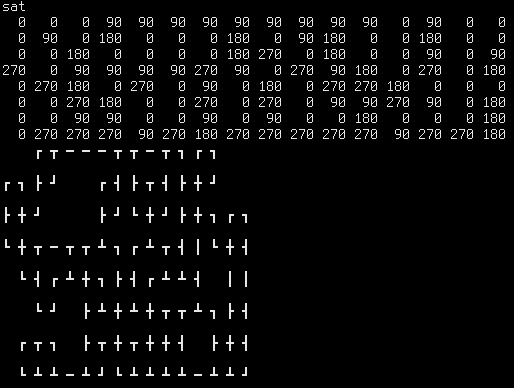
\includegraphics[scale=0.75]{\CURPATH/solver/solver.png}
\caption{Вывод скрипта солвера}
\end{figure}

Это работает $\approx 4$ секунды на моем старом и медленном Intel Atom N455 1.66GHz.
Быстро ли это? Не знаю, но снова вот что действительно круто, это то что мы понятия не имеем о какой-то математической
теории за всем этим, мы просто объявили ячейки, (полу-)стыки и определили отношения между ними.

Теперь следующий вопрос это, сколько здесь возможных решений?
Используя раннее описанный метод (\ref{SMTEnumerate}), я немного изменил скрипт солвера
\footnote{\url{.../solver/solve_pipe_puzzle2.py}} и солвер
сказал что возможно два решения.

Сравним их используя gvimdiff:

\begin{figure}[H]
\centering
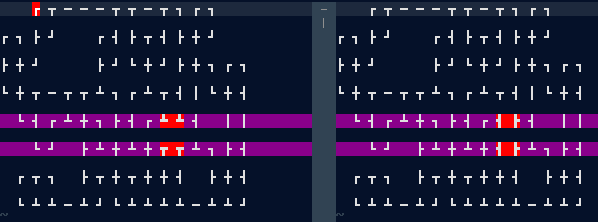
\includegraphics[scale=0.75]{\CURPATH/solver/diff.png}
\caption{Вывод gvimdiff (извините за мой красный курсор в левой части в левом верхнем углу)}
\end{figure}

4 ячейки в середине могут быть ориентированы по-разному.
Видимо, другие головоломки могут также выдавать разные результаты.

P.S.
\textit{Полу-стык} определен как булевый тип.
Но на самом деле, первая версия солвера была написана используя целочисленный тип для полу-стыков,
и 0 использовалось для False и 1 для True.
Я так сделал, потому что хотел более компактный исходный код, без использования длинных слов как ``False'' и ``True''.
И это работало, но медленнее. Вероятно, Z3 работает с булевыми типами быстрее? Лучше?
Так или иначе, я пишу это чтобы отметить, что, если нужно, целочисленный тип можно использовать вместо булевого.


\section{Развлекательная математика и головоломки}

\input{puzzles/sudoku/main_RU}
\input{puzzles/zebra/main_RU}
\input{puzzles/pipe/main_RU}
\input{puzzles/rubik2/failed_SMT/main_RU}
\input{puzzles/rubik2/SAT/main_RU}
\input{puzzles/rubik3/one_face_SMT/main_RU}
%\input{puzzles/numberlink/main_RU}
%\input{puzzles/two_parks_RU}
\input{puzzles/alphametics/main_RU}
%\input{puzzles/2015_AIME_II_Problems_12_RU}
%\input{puzzles/fred/main_RU}
%\input{puzzles/MC/main_RU}
%\input{puzzles/coin_flip/main_RU}
%\input{puzzles/Mock_AIME_2_2006-2007_Problem_8_RU}
%\input{puzzles/2012_AIME_I_Problems_1_RU}
%\input{puzzles/keypad_RU}


\section{Развлекательная математика и головоломки}

\input{puzzles/sudoku/main_RU}
\input{puzzles/zebra/main_RU}
\input{puzzles/pipe/main_RU}
\input{puzzles/rubik2/failed_SMT/main_RU}
\input{puzzles/rubik2/SAT/main_RU}
\input{puzzles/rubik3/one_face_SMT/main_RU}
%\input{puzzles/numberlink/main_RU}
%\input{puzzles/two_parks_RU}
\input{puzzles/alphametics/main_RU}
%\input{puzzles/2015_AIME_II_Problems_12_RU}
%\input{puzzles/fred/main_RU}
%\input{puzzles/MC/main_RU}
%\input{puzzles/coin_flip/main_RU}
%\input{puzzles/Mock_AIME_2_2006-2007_Problem_8_RU}
%\input{puzzles/2012_AIME_I_Problems_1_RU}
%\input{puzzles/keypad_RU}


\section{Развлекательная математика и головоломки}

\input{puzzles/sudoku/main_RU}
\input{puzzles/zebra/main_RU}
\input{puzzles/pipe/main_RU}
\input{puzzles/rubik2/failed_SMT/main_RU}
\input{puzzles/rubik2/SAT/main_RU}
\input{puzzles/rubik3/one_face_SMT/main_RU}
%\input{puzzles/numberlink/main_RU}
%\input{puzzles/two_parks_RU}
\input{puzzles/alphametics/main_RU}
%\input{puzzles/2015_AIME_II_Problems_12_RU}
%\input{puzzles/fred/main_RU}
%\input{puzzles/MC/main_RU}
%\input{puzzles/coin_flip/main_RU}
%\input{puzzles/Mock_AIME_2_2006-2007_Problem_8_RU}
%\input{puzzles/2012_AIME_I_Problems_1_RU}
%\input{puzzles/keypad_RU}


%\section{Развлекательная математика и головоломки}

\input{puzzles/sudoku/main_RU}
\input{puzzles/zebra/main_RU}
\input{puzzles/pipe/main_RU}
\input{puzzles/rubik2/failed_SMT/main_RU}
\input{puzzles/rubik2/SAT/main_RU}
\input{puzzles/rubik3/one_face_SMT/main_RU}
%\input{puzzles/numberlink/main_RU}
%\input{puzzles/two_parks_RU}
\input{puzzles/alphametics/main_RU}
%\input{puzzles/2015_AIME_II_Problems_12_RU}
%\input{puzzles/fred/main_RU}
%\input{puzzles/MC/main_RU}
%\input{puzzles/coin_flip/main_RU}
%\input{puzzles/Mock_AIME_2_2006-2007_Problem_8_RU}
%\input{puzzles/2012_AIME_I_Problems_1_RU}
%\input{puzzles/keypad_RU}


%\input{puzzles/two_parks_RU}
\subsection{Альфаметика}

Согласно Дональду Кнуту, термин ``Альфаметика'' был придуман Дж. Эйч. Аш. Хантером.
Это головоломка: какие десятичные цифры в пределах 0..9 нужно присвоить каждой букве, чтобы это уравнение было справедливо?

\begin{lstlisting}
  SEND
+ MORE
 -----
 MONEY
\end{lstlisting}

Для Z3 это легко:

\lstinputlisting{puzzles/alphametics/alpha.py}

Вывод:

\begin{lstlisting}
sat
[E, = 5,
 S, = 9,
 M, = 1,
 N, = 6,
 D, = 7,
 R, = 8,
 O, = 0,
 Y = 2]
\end{lstlisting}

Вот еще одна, из \ac{TAOCP} том IV (\url{http://www-cs-faculty.stanford.edu/~uno/fasc2b.ps.gz}):

\lstinputlisting{puzzles/alphametics/alpha2.py}

\begin{lstlisting}
sat
[L, = 6,
 S, = 7,
 N, = 2,
 T, = 1,
 I, = 5,
 V = 3,
 A, = 8,
 R, = 9,
 O, = 4,
 TRIO = 1954,
 SONATA, = 742818,
 VIOLA, = 35468,
 VIOLIN, = 354652]
\end{lstlisting}

% TODO URL
Эту головоломку я нашел в примерах pySMT:

\lstinputlisting{puzzles/alphametics/alpha3.py}

\begin{lstlisting}
sat
[D = 5, R = 4, O = 3, E = 8, L = 6, W = 7, H = 2]
\end{lstlisting}

%%% 

Это упражнение Q209 из
[Companion to the Papers of Donald Knuth]\footnote{\url{http://www-cs-faculty.stanford.edu/~knuth/cp.html}}.

\begin{lstlisting}
 KNIFE
  FORK
 SPOON
  SOUP
------
SUPPER
\end{lstlisting}

В целях упрощения, я добавил ф-цию (list\_to\_expr()):

\lstinputlisting{puzzles/alphametics/alpha4.py}

\begin{lstlisting}
sat
[K = 7,
 N = 4,
 R = 9,
 I = 1,
 E = 6,
 S = 0,
 O = 3,
 F = 5,
 U = 8,
 P = 2,
 SUPPER = 82269,
 SOUP = 382,
 SPOON = 2334,
 FORK = 5397,
 KNIFE = 74156]
\end{lstlisting}

S это 0, так что значение SUPPER начинается с (убранного) нуля. Скажем так, нам это не нравится.
Добавим это, чтобы это исправить:

\begin{lstlisting}
s.add(S!=0)
\end{lstlisting}

\begin{lstlisting}
sat
[K = 8,
 N = 4,
 R = 3,
 I = 7,
 E = 6,
 S = 1,
 O = 9,
 F = 2,
 U = 0,
 P = 5,
 SUPPER = 105563,
 SOUP = 1905,
 SPOON = 15994,
 FORK = 2938,
 KNIFE = 84726]
\end{lstlisting}

\paragraph{Создание своей собственной головоломки}

Вот проблема: есть только 10 букв, но как их выбрать из числа слов?
Мы можем использовать Z3 для этого:

\lstinputlisting{puzzles/alphametics/gen.py}

Это первая сгенерированная головоломка:

\begin{lstlisting}
sat
EGGS
JELLY
LUNCH
C 5
E 6
G 3
H 7
J 0
L 1
N 4
S 8
U 2
Y 9
\end{lstlisting}

Что если мы хотим, чтобы слово ``CAKE'' присутствовало в числе ``слагаемых''?

Добавим это:

\begin{lstlisting}
s.add(word_used[words.index('CAKE')])
\end{lstlisting}

\begin{lstlisting}
sat
CAKE
TEA
LUNCH
A 8
C 3
E 1
H 9
J 6
K 2
L 0
N 5
T 7
U 4
\end{lstlisting}

Добавим это:

\begin{lstlisting}
s.add(word_used[words.index('EGGS')])
\end{lstlisting}

Теперь оно может найти пару к EGGS:

\begin{lstlisting}
sat
EGGS
HONEY
LUNCH
C 6
E 7
G 9
H 4
L 5
N 8
O 2
S 3
U 0
Y 1
\end{lstlisting}

\paragraph{Файлы}

\url{https://github.com/DennisYurichev/...}




%\input{puzzles/2015_AIME_II_Problems_12_RU}
%\section{Развлекательная математика и головоломки}

\input{puzzles/sudoku/main_RU}
\input{puzzles/zebra/main_RU}
\input{puzzles/pipe/main_RU}
\input{puzzles/rubik2/failed_SMT/main_RU}
\input{puzzles/rubik2/SAT/main_RU}
\input{puzzles/rubik3/one_face_SMT/main_RU}
%\input{puzzles/numberlink/main_RU}
%\input{puzzles/two_parks_RU}
\input{puzzles/alphametics/main_RU}
%\input{puzzles/2015_AIME_II_Problems_12_RU}
%\input{puzzles/fred/main_RU}
%\input{puzzles/MC/main_RU}
%\input{puzzles/coin_flip/main_RU}
%\input{puzzles/Mock_AIME_2_2006-2007_Problem_8_RU}
%\input{puzzles/2012_AIME_I_Problems_1_RU}
%\input{puzzles/keypad_RU}


%\section{Развлекательная математика и головоломки}

\input{puzzles/sudoku/main_RU}
\input{puzzles/zebra/main_RU}
\input{puzzles/pipe/main_RU}
\input{puzzles/rubik2/failed_SMT/main_RU}
\input{puzzles/rubik2/SAT/main_RU}
\input{puzzles/rubik3/one_face_SMT/main_RU}
%\input{puzzles/numberlink/main_RU}
%\input{puzzles/two_parks_RU}
\input{puzzles/alphametics/main_RU}
%\input{puzzles/2015_AIME_II_Problems_12_RU}
%\input{puzzles/fred/main_RU}
%\input{puzzles/MC/main_RU}
%\input{puzzles/coin_flip/main_RU}
%\input{puzzles/Mock_AIME_2_2006-2007_Problem_8_RU}
%\input{puzzles/2012_AIME_I_Problems_1_RU}
%\input{puzzles/keypad_RU}


%\section{Развлекательная математика и головоломки}

\input{puzzles/sudoku/main_RU}
\input{puzzles/zebra/main_RU}
\input{puzzles/pipe/main_RU}
\input{puzzles/rubik2/failed_SMT/main_RU}
\input{puzzles/rubik2/SAT/main_RU}
\input{puzzles/rubik3/one_face_SMT/main_RU}
%\input{puzzles/numberlink/main_RU}
%\input{puzzles/two_parks_RU}
\input{puzzles/alphametics/main_RU}
%\input{puzzles/2015_AIME_II_Problems_12_RU}
%\input{puzzles/fred/main_RU}
%\input{puzzles/MC/main_RU}
%\input{puzzles/coin_flip/main_RU}
%\input{puzzles/Mock_AIME_2_2006-2007_Problem_8_RU}
%\input{puzzles/2012_AIME_I_Problems_1_RU}
%\input{puzzles/keypad_RU}


%\input{puzzles/Mock_AIME_2_2006-2007_Problem_8_RU}
%\input{puzzles/2012_AIME_I_Problems_1_RU}
%\input{puzzles/keypad_RU}


\section{Развлекательная математика и головоломки}

\subsection{Судоку}

Головоломка Судоку это решетка 9*9, некоторые ячейки заполнены значениями, некоторые пустые:

% copypasted from http://www.texample.net/tikz/examples/sudoku/
\newcounter{row}
\newcounter{col}

\newcommand\setrow[9]{
  \setcounter{col}{1}
  \foreach \n in {#1, #2, #3, #4, #5, #6, #7, #8, #9} {
    \edef\x{\value{col} - 0.5}
    \edef\y{9.5 - \value{row}}
    \node[anchor=center] at (\x, \y) {\n};
    \stepcounter{col}
  }
  \stepcounter{row}
}

\begin{center}
\begin{tikzpicture}[scale=.7]
  \begin{scope}
    \draw (0, 0) grid (9, 9);
    \draw[very thick, scale=3] (0, 0) grid (3, 3);

    \setcounter{row}{1}
    \setrow { }{ }{5}  {3}{ }{ }  { }{ }{ }
    \setrow {8}{ }{ }  { }{ }{ }  { }{2}{ }
    \setrow { }{7}{ }  { }{1}{ }  {5}{ }{ }

    \setrow {4}{ }{ }  { }{ }{5}  {3}{ }{ }
    \setrow { }{1}{ }  { }{7}{ }  { }{ }{6}
    \setrow { }{ }{3}  {2}{ }{ }  { }{8}{ }

    \setrow { }{6}{ }  {5}{ }{ }  { }{ }{9}
    \setrow { }{ }{4}  { }{ }{ }  { }{3}{ }
    \setrow { }{ }{ }  { }{ }{9}  {7}{ }{ }

    \node[anchor=center] at (4.5, -0.5) {Нерешенная Судоку};
  \end{scope}
\end{tikzpicture}
\end{center}

Числа в каждом ряду должны быть уникальными, т.е., каждый ряд должен содержать 9 чисел в пределах 1..9 без повторений.
Та же история и для каждого столбца и каждого квадрата 3*3.

Головоломка представляет собой хороший кандидат, на котором можно попробовать \ac{SMT}-солвер, потому что это,
в общем-то, просто нерешенная система уравнений.

\input{puzzles/sudoku/1/main_RU}
%\input{puzzles/sudoku/GT/main_RU}
%\input{puzzles/sudoku/killer/main_RU}
\input{puzzles/sudoku/KLEE/main_RU}
\input{puzzles/sudoku/SAT/main_RU}


\subsection{Головоломка зебры (\ac{AKA} Загадка Эйнштейна)}

\input{puzzles/zebra/SMT/main_RU}
\input{puzzles/zebra/KLEE/main_RU}
\input{puzzles/zebra/SAT/main_RU}


\subsection{Решение головоломки ``трубы'' используя Z3 SMT-солвер}

\renewcommand{\CURPATH}{puzzles/pipe}

Головоломка ``трубы'' это популярная головоломка (просто погуглите ``pipe puzzle'' и посмотрите на картинки).

Вот как выглядит головоломка в разобранном виде:

\begin{figure}[H]
\label{fig:pipe_shuffled}
\centering
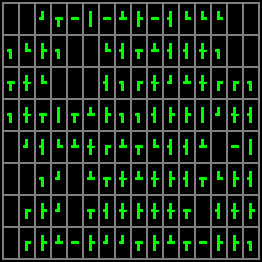
\includegraphics[scale=0.75]{\CURPATH/shuffled.png}
\caption{Разобранная головоломка}
\end{figure}

\dots и собранная:

\begin{figure}[H]
\label{fig:pipe_solved}
\centering
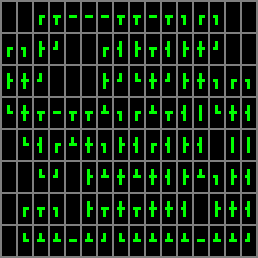
\includegraphics[scale=0.75]{\CURPATH/solved.png}
\caption{Собранная головоломка}
\end{figure}

Попробуем найти способ собрать её.

\subsubsection{Создание}

В начале, нужно её создать.
Вот простая идея.
Возьем массив ячеек 8*16.
Каждая ячейка может содержать какой-то тип блока.
Между ячейками есть стыки:

\input{\CURPATH/pipe_gen.tex}

Синие линии это горизонтальные стыки, красные линии это вертикальные стыки.
Мы просто случайно выставляем каждый стык в 0/false (отсутствует) или 1/true (присутствует).

После этого, теперь легко найти тип каждой ячейки.
А это:

\newcommand{\HeaderColor}{\cellcolor{blue!25}}
\begin{center}
\begin{longtable}{ | l | l | l | l | }
\hline
\HeaderColor стыки & \HeaderColor наше внутреннее название & \HeaderColor угол & \HeaderColor символ \\
\hline
0	&type 0		&	0$^{\circ}$	& (пробел)	\\
2	&type 2a	&	0$^{\circ}$	& \pmboxdrawuni{2503} \\ % ┃
2	&type 2a	&	90$^{\circ}$	& \pmboxdrawuni{2501} \\ % ━
2	&type 2b	&	0$^{\circ}$	& \pmboxdrawuni{250F} \\ % ┏
2	&type 2b	&	90$^{\circ}$	& \pmboxdrawuni{2513} \\ % ┓
2	&type 2b	&	180$^{\circ}$	& \pmboxdrawuni{251B} \\ % ┛
2	&type 2b	&	270$^{\circ}$	& \pmboxdrawuni{2517} \\ % ┗
3	&type 3		&	0$^{\circ}$	& \pmboxdrawuni{2523} \\ % ┣
3 	&type 3		&	90$^{\circ}$	& \pmboxdrawuni{2533} \\ % ┳
3	&type 3		&	180$^{\circ}$	& \pmboxdrawuni{252B} \\ % ┫
3	&type 3		&	270$^{\circ}$	& \pmboxdrawuni{253B} \\ % ┻
4	&type 4		&	0$^{\circ}$	& \pmboxdrawuni{254B} \\ % ╋
\hline
\end{longtable}
\end{center}

\textit{Висящие} стыки могут присутствовать на первой стадии (т.е., ячейки только с одним стыком), но они удалются
рекурсивно, и эти ячейки преобразуются в пустые ячейки.
Так что, в самом конце, все ячейки имеют минимум 2 стыка, и вся эта сантехническая система не имеет связей с внешним миром ---
я надеюсь, из-за этого станет немного проще.

Исходник генератора на Си здесь: \url{.../pipe/generator}.
Все вертикальные стыки хранятся в глобальном массиве \textit{hjoints[]} и вертикальные в \textit{vjoints[]}.

Программа на Си генерирует ANSI-раскрашенный вывод, как это было показано выше
(\ref{fig:pipe_shuffled}, \ref{fig:pipe_solved}) плюс массив типов для каждой ячейки, но без информации об углах:

\begin{lstlisting}[label=init_cells]
[
["0", "0", "2b", "3", "2a", "2a", "2a", "3", "3", "2a", "3", "2b", "2b", "2b", "0", "0"],
["2b", "2b", "3", "2b", "0", "0", "2b", "3", "3", "3", "3", "3", "4", "2b", "0", "0"],
["3", "4", "2b", "0", "0", "0", "3", "2b", "2b", "4", "2b", "3", "4", "2b", "2b", "2b"],
["2b", "4", "3", "2a", "3", "3", "3", "2b", "2b", "3", "3", "3", "2a", "2b", "4", "3"],
["0", "2b", "3", "2b", "3", "4", "2b", "3", "3", "2b", "3", "3", "3", "0", "2a", "2a"],
["0", "0", "2b", "2b", "0", "3", "3", "4", "3", "4", "3", "3", "3", "2b", "3", "3"],
["0", "2b", "3", "2b", "0", "3", "3", "4", "3", "4", "4", "3", "0", "3", "4", "3"],
["0", "2b", "3", "3", "2a", "3", "2b", "2b", "3", "3", "3", "3", "2a", "3", "3", "2b"],
]
\end{lstlisting}

\subsubsection{Решение}

Прежде всего, мы будем работать с массивом ячеек 8*16, где каждый элемент имеет 4 бита:
``T'' (top/верх),
``B'' (bottom/низ),
``L'' (left/лево),
``R'' (right/право).
Каждый бит представляет собой половину стыка.

\input{\CURPATH/pipe_solve.tex}

Теперь определяем массив для каждого из четырех полустыков + информация об угле:

\begin{lstlisting}
HEIGHT=8
WIDTH=16

# if T/B/R/L is Bool instead of Int, Z3 solver will work faster
T=[[Bool('cell_%d_%d_top' % (r, c)) for c in range(WIDTH)] for r in range(HEIGHT)]
B=[[Bool('cell_%d_%d_bottom' % (r, c)) for c in range(WIDTH)] for r in range(HEIGHT)]
R=[[Bool('cell_%d_%d_right' % (r, c)) for c in range(WIDTH)] for r in range(HEIGHT)]
L=[[Bool('cell_%d_%d_left' % (r, c)) for c in range(WIDTH)] for r in range(HEIGHT)]
A=[[Int('cell_%d_%d_angle' % (r, c)) for c in range(WIDTH)] for r in range(HEIGHT)]
\end{lstlisting}

Мы знаем, что если каждый из полустыков присутствует, ответный полустык также должен присутствовать, и наоборот. 
Определяем всё это используя эти констрайнты:

\begin{lstlisting}
# shorthand variables for True and False:
t=True
f=False

# "top" of each cell must be equal to "bottom" of the cell above
# "bottom" of each cell must be equal to "top" of the cell below
# "left" of each cell must be equal to "right" of the cell at left
# "right" of each cell must be equal to "left" of the cell at right
for r in range(HEIGHT):
    for c in range(WIDTH):
        if r!=0:
            s.add(T[r][c]==B[r-1][c])
        if r!=HEIGHT-1:
            s.add(B[r][c]==T[r+1][c])
        if c!=0:
            s.add(L[r][c]==R[r][c-1])
        if c!=WIDTH-1:
            s.add(R[r][c]==L[r][c+1])

# "left" of each cell of first column shouldn't have any connection
# so is "right" of each cell of the last column
for r in range(HEIGHT):
    s.add(L[r][0]==f)
    s.add(R[r][WIDTH-1]==f)

# "top" of each cell of the first row shouldn't have any connection
# so is "bottom" of each cell of the last row
for c in range(WIDTH):
    s.add(T[0][c]==f)
    s.add(B[HEIGHT-1][c]==f)
\end{lstlisting}

Теперь перебираем все ячейки в изначальном массиве (\ref{init_cells}).
Первые две ячейки здесь пустые. И третья имеет тип ``2b''.
Это ``\pmboxdrawuni{250F}'' % ┏
и его можно ориентировать четырьмя разными способами.
И если её угол это 0$^{\circ}$, верхний и правый полустыки присутствуют, остальные отсутствуют.
Если он имеет угол 90$^{\circ}$, он выглядит как 
``\pmboxdrawuni{2513}'', % ┓
и верхник и левый полустыки присутствуют, остальные отсутствуют.

На обычном русском языке: ``если ячейка этого типа имеет угол 0$^{\circ}$, вот эти полустыки должны присутствовать \textbf{ИЛИ}
если она имеет угол 90$^{\circ}$, эти полустыки должны присутствовать, \textbf{ИЛИ}, итд, итд.''

Точно также, мы определяем эти правила для всех типов и всех возможных углов:

\begin{lstlisting}
for r in range(HEIGHT):
    for c in range(WIDTH):
        ty=cells_type[r][c]

        if ty=="0":
            s.add(A[r][c]==f)
            s.add(T[r][c]==f, B[r][c]==f, L[r][c]==f, R[r][c]==f)

        if ty=="2a":
            s.add(Or(And(A[r][c]==0, L[r][c]==f, R[r][c]==f, T[r][c]==t, B[r][c]==t),   # §\pmboxdrawuni{2503}§
                    And(A[r][c]==90, L[r][c]==t, R[r][c]==t, T[r][c]==f, B[r][c]==f)))  # §\pmboxdrawuni{2501}§

        if ty=="2b":
            s.add(Or(And(A[r][c]==0, L[r][c]==f, R[r][c]==t, T[r][c]==f, B[r][c]==t),   # §\pmboxdrawuni{250F}§
                    And(A[r][c]==90, L[r][c]==t, R[r][c]==f, T[r][c]==f, B[r][c]==t),   # §\pmboxdrawuni{2513}§
                    And(A[r][c]==180, L[r][c]==t, R[r][c]==f, T[r][c]==t, B[r][c]==f),  # §\pmboxdrawuni{251B}§
                    And(A[r][c]==270, L[r][c]==f, R[r][c]==t, T[r][c]==t, B[r][c]==f))) # §\pmboxdrawuni{2517}§
	
        if ty=="3":
            s.add(Or(And(A[r][c]==0, L[r][c]==f, R[r][c]==t, T[r][c]==t, B[r][c]==t),   # §\pmboxdrawuni{2523}§
                    And(A[r][c]==90, L[r][c]==t, R[r][c]==t, T[r][c]==f, B[r][c]==t),   # §\pmboxdrawuni{2533}§
                    And(A[r][c]==180, L[r][c]==t, R[r][c]==f, T[r][c]==t, B[r][c]==t),  # §\pmboxdrawuni{252B}§
                    And(A[r][c]==270, L[r][c]==t, R[r][c]==t, T[r][c]==t, B[r][c]==f))) # §\pmboxdrawuni{253B}§

        if ty=="4":
            s.add(A[r][c]==0)
            s.add(T[r][c]==t, B[r][c]==t, L[r][c]==t, R[r][c]==t) # §\pmboxdrawuni{254B}§
\end{lstlisting}

Полный исходник здесь: \url{.../solver/solve_pipe_puzzle1.py}.

Получается такой результат (выводит угол для каждой ячейки и (псевдо)графическое представление):

\begin{figure}[H]
\centering
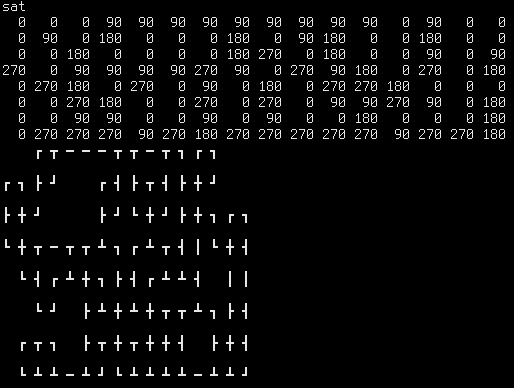
\includegraphics[scale=0.75]{\CURPATH/solver/solver.png}
\caption{Вывод скрипта солвера}
\end{figure}

Это работает $\approx 4$ секунды на моем старом и медленном Intel Atom N455 1.66GHz.
Быстро ли это? Не знаю, но снова вот что действительно круто, это то что мы понятия не имеем о какой-то математической
теории за всем этим, мы просто объявили ячейки, (полу-)стыки и определили отношения между ними.

Теперь следующий вопрос это, сколько здесь возможных решений?
Используя раннее описанный метод (\ref{SMTEnumerate}), я немного изменил скрипт солвера
\footnote{\url{.../solver/solve_pipe_puzzle2.py}} и солвер
сказал что возможно два решения.

Сравним их используя gvimdiff:

\begin{figure}[H]
\centering
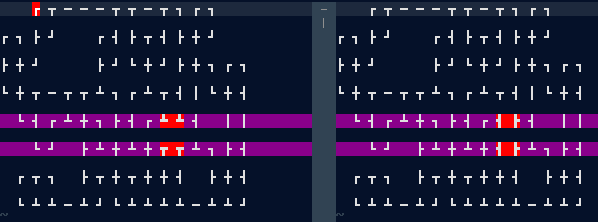
\includegraphics[scale=0.75]{\CURPATH/solver/diff.png}
\caption{Вывод gvimdiff (извините за мой красный курсор в левой части в левом верхнем углу)}
\end{figure}

4 ячейки в середине могут быть ориентированы по-разному.
Видимо, другие головоломки могут также выдавать разные результаты.

P.S.
\textit{Полу-стык} определен как булевый тип.
Но на самом деле, первая версия солвера была написана используя целочисленный тип для полу-стыков,
и 0 использовалось для False и 1 для True.
Я так сделал, потому что хотел более компактный исходный код, без использования длинных слов как ``False'' и ``True''.
И это работало, но медленнее. Вероятно, Z3 работает с булевыми типами быстрее? Лучше?
Так или иначе, я пишу это чтобы отметить, что, если нужно, целочисленный тип можно использовать вместо булевого.


\section{Развлекательная математика и головоломки}

\input{puzzles/sudoku/main_RU}
\input{puzzles/zebra/main_RU}
\input{puzzles/pipe/main_RU}
\input{puzzles/rubik2/failed_SMT/main_RU}
\input{puzzles/rubik2/SAT/main_RU}
\input{puzzles/rubik3/one_face_SMT/main_RU}
%\input{puzzles/numberlink/main_RU}
%\input{puzzles/two_parks_RU}
\input{puzzles/alphametics/main_RU}
%\input{puzzles/2015_AIME_II_Problems_12_RU}
%\input{puzzles/fred/main_RU}
%\input{puzzles/MC/main_RU}
%\input{puzzles/coin_flip/main_RU}
%\input{puzzles/Mock_AIME_2_2006-2007_Problem_8_RU}
%\input{puzzles/2012_AIME_I_Problems_1_RU}
%\input{puzzles/keypad_RU}


\section{Развлекательная математика и головоломки}

\input{puzzles/sudoku/main_RU}
\input{puzzles/zebra/main_RU}
\input{puzzles/pipe/main_RU}
\input{puzzles/rubik2/failed_SMT/main_RU}
\input{puzzles/rubik2/SAT/main_RU}
\input{puzzles/rubik3/one_face_SMT/main_RU}
%\input{puzzles/numberlink/main_RU}
%\input{puzzles/two_parks_RU}
\input{puzzles/alphametics/main_RU}
%\input{puzzles/2015_AIME_II_Problems_12_RU}
%\input{puzzles/fred/main_RU}
%\input{puzzles/MC/main_RU}
%\input{puzzles/coin_flip/main_RU}
%\input{puzzles/Mock_AIME_2_2006-2007_Problem_8_RU}
%\input{puzzles/2012_AIME_I_Problems_1_RU}
%\input{puzzles/keypad_RU}


\section{Развлекательная математика и головоломки}

\input{puzzles/sudoku/main_RU}
\input{puzzles/zebra/main_RU}
\input{puzzles/pipe/main_RU}
\input{puzzles/rubik2/failed_SMT/main_RU}
\input{puzzles/rubik2/SAT/main_RU}
\input{puzzles/rubik3/one_face_SMT/main_RU}
%\input{puzzles/numberlink/main_RU}
%\input{puzzles/two_parks_RU}
\input{puzzles/alphametics/main_RU}
%\input{puzzles/2015_AIME_II_Problems_12_RU}
%\input{puzzles/fred/main_RU}
%\input{puzzles/MC/main_RU}
%\input{puzzles/coin_flip/main_RU}
%\input{puzzles/Mock_AIME_2_2006-2007_Problem_8_RU}
%\input{puzzles/2012_AIME_I_Problems_1_RU}
%\input{puzzles/keypad_RU}


%\section{Развлекательная математика и головоломки}

\input{puzzles/sudoku/main_RU}
\input{puzzles/zebra/main_RU}
\input{puzzles/pipe/main_RU}
\input{puzzles/rubik2/failed_SMT/main_RU}
\input{puzzles/rubik2/SAT/main_RU}
\input{puzzles/rubik3/one_face_SMT/main_RU}
%\input{puzzles/numberlink/main_RU}
%\input{puzzles/two_parks_RU}
\input{puzzles/alphametics/main_RU}
%\input{puzzles/2015_AIME_II_Problems_12_RU}
%\input{puzzles/fred/main_RU}
%\input{puzzles/MC/main_RU}
%\input{puzzles/coin_flip/main_RU}
%\input{puzzles/Mock_AIME_2_2006-2007_Problem_8_RU}
%\input{puzzles/2012_AIME_I_Problems_1_RU}
%\input{puzzles/keypad_RU}


%\input{puzzles/two_parks_RU}
\subsection{Альфаметика}

Согласно Дональду Кнуту, термин ``Альфаметика'' был придуман Дж. Эйч. Аш. Хантером.
Это головоломка: какие десятичные цифры в пределах 0..9 нужно присвоить каждой букве, чтобы это уравнение было справедливо?

\begin{lstlisting}
  SEND
+ MORE
 -----
 MONEY
\end{lstlisting}

Для Z3 это легко:

\lstinputlisting{puzzles/alphametics/alpha.py}

Вывод:

\begin{lstlisting}
sat
[E, = 5,
 S, = 9,
 M, = 1,
 N, = 6,
 D, = 7,
 R, = 8,
 O, = 0,
 Y = 2]
\end{lstlisting}

Вот еще одна, из \ac{TAOCP} том IV (\url{http://www-cs-faculty.stanford.edu/~uno/fasc2b.ps.gz}):

\lstinputlisting{puzzles/alphametics/alpha2.py}

\begin{lstlisting}
sat
[L, = 6,
 S, = 7,
 N, = 2,
 T, = 1,
 I, = 5,
 V = 3,
 A, = 8,
 R, = 9,
 O, = 4,
 TRIO = 1954,
 SONATA, = 742818,
 VIOLA, = 35468,
 VIOLIN, = 354652]
\end{lstlisting}

% TODO URL
Эту головоломку я нашел в примерах pySMT:

\lstinputlisting{puzzles/alphametics/alpha3.py}

\begin{lstlisting}
sat
[D = 5, R = 4, O = 3, E = 8, L = 6, W = 7, H = 2]
\end{lstlisting}

%%% 

Это упражнение Q209 из
[Companion to the Papers of Donald Knuth]\footnote{\url{http://www-cs-faculty.stanford.edu/~knuth/cp.html}}.

\begin{lstlisting}
 KNIFE
  FORK
 SPOON
  SOUP
------
SUPPER
\end{lstlisting}

В целях упрощения, я добавил ф-цию (list\_to\_expr()):

\lstinputlisting{puzzles/alphametics/alpha4.py}

\begin{lstlisting}
sat
[K = 7,
 N = 4,
 R = 9,
 I = 1,
 E = 6,
 S = 0,
 O = 3,
 F = 5,
 U = 8,
 P = 2,
 SUPPER = 82269,
 SOUP = 382,
 SPOON = 2334,
 FORK = 5397,
 KNIFE = 74156]
\end{lstlisting}

S это 0, так что значение SUPPER начинается с (убранного) нуля. Скажем так, нам это не нравится.
Добавим это, чтобы это исправить:

\begin{lstlisting}
s.add(S!=0)
\end{lstlisting}

\begin{lstlisting}
sat
[K = 8,
 N = 4,
 R = 3,
 I = 7,
 E = 6,
 S = 1,
 O = 9,
 F = 2,
 U = 0,
 P = 5,
 SUPPER = 105563,
 SOUP = 1905,
 SPOON = 15994,
 FORK = 2938,
 KNIFE = 84726]
\end{lstlisting}

\paragraph{Создание своей собственной головоломки}

Вот проблема: есть только 10 букв, но как их выбрать из числа слов?
Мы можем использовать Z3 для этого:

\lstinputlisting{puzzles/alphametics/gen.py}

Это первая сгенерированная головоломка:

\begin{lstlisting}
sat
EGGS
JELLY
LUNCH
C 5
E 6
G 3
H 7
J 0
L 1
N 4
S 8
U 2
Y 9
\end{lstlisting}

Что если мы хотим, чтобы слово ``CAKE'' присутствовало в числе ``слагаемых''?

Добавим это:

\begin{lstlisting}
s.add(word_used[words.index('CAKE')])
\end{lstlisting}

\begin{lstlisting}
sat
CAKE
TEA
LUNCH
A 8
C 3
E 1
H 9
J 6
K 2
L 0
N 5
T 7
U 4
\end{lstlisting}

Добавим это:

\begin{lstlisting}
s.add(word_used[words.index('EGGS')])
\end{lstlisting}

Теперь оно может найти пару к EGGS:

\begin{lstlisting}
sat
EGGS
HONEY
LUNCH
C 6
E 7
G 9
H 4
L 5
N 8
O 2
S 3
U 0
Y 1
\end{lstlisting}

\paragraph{Файлы}

\url{https://github.com/DennisYurichev/...}




%\input{puzzles/2015_AIME_II_Problems_12_RU}
%\section{Развлекательная математика и головоломки}

\input{puzzles/sudoku/main_RU}
\input{puzzles/zebra/main_RU}
\input{puzzles/pipe/main_RU}
\input{puzzles/rubik2/failed_SMT/main_RU}
\input{puzzles/rubik2/SAT/main_RU}
\input{puzzles/rubik3/one_face_SMT/main_RU}
%\input{puzzles/numberlink/main_RU}
%\input{puzzles/two_parks_RU}
\input{puzzles/alphametics/main_RU}
%\input{puzzles/2015_AIME_II_Problems_12_RU}
%\input{puzzles/fred/main_RU}
%\input{puzzles/MC/main_RU}
%\input{puzzles/coin_flip/main_RU}
%\input{puzzles/Mock_AIME_2_2006-2007_Problem_8_RU}
%\input{puzzles/2012_AIME_I_Problems_1_RU}
%\input{puzzles/keypad_RU}


%\section{Развлекательная математика и головоломки}

\input{puzzles/sudoku/main_RU}
\input{puzzles/zebra/main_RU}
\input{puzzles/pipe/main_RU}
\input{puzzles/rubik2/failed_SMT/main_RU}
\input{puzzles/rubik2/SAT/main_RU}
\input{puzzles/rubik3/one_face_SMT/main_RU}
%\input{puzzles/numberlink/main_RU}
%\input{puzzles/two_parks_RU}
\input{puzzles/alphametics/main_RU}
%\input{puzzles/2015_AIME_II_Problems_12_RU}
%\input{puzzles/fred/main_RU}
%\input{puzzles/MC/main_RU}
%\input{puzzles/coin_flip/main_RU}
%\input{puzzles/Mock_AIME_2_2006-2007_Problem_8_RU}
%\input{puzzles/2012_AIME_I_Problems_1_RU}
%\input{puzzles/keypad_RU}


%\section{Развлекательная математика и головоломки}

\input{puzzles/sudoku/main_RU}
\input{puzzles/zebra/main_RU}
\input{puzzles/pipe/main_RU}
\input{puzzles/rubik2/failed_SMT/main_RU}
\input{puzzles/rubik2/SAT/main_RU}
\input{puzzles/rubik3/one_face_SMT/main_RU}
%\input{puzzles/numberlink/main_RU}
%\input{puzzles/two_parks_RU}
\input{puzzles/alphametics/main_RU}
%\input{puzzles/2015_AIME_II_Problems_12_RU}
%\input{puzzles/fred/main_RU}
%\input{puzzles/MC/main_RU}
%\input{puzzles/coin_flip/main_RU}
%\input{puzzles/Mock_AIME_2_2006-2007_Problem_8_RU}
%\input{puzzles/2012_AIME_I_Problems_1_RU}
%\input{puzzles/keypad_RU}


%\input{puzzles/Mock_AIME_2_2006-2007_Problem_8_RU}
%\input{puzzles/2012_AIME_I_Problems_1_RU}
%\input{puzzles/keypad_RU}


%\section{Развлекательная математика и головоломки}

\subsection{Судоку}

Головоломка Судоку это решетка 9*9, некоторые ячейки заполнены значениями, некоторые пустые:

% copypasted from http://www.texample.net/tikz/examples/sudoku/
\newcounter{row}
\newcounter{col}

\newcommand\setrow[9]{
  \setcounter{col}{1}
  \foreach \n in {#1, #2, #3, #4, #5, #6, #7, #8, #9} {
    \edef\x{\value{col} - 0.5}
    \edef\y{9.5 - \value{row}}
    \node[anchor=center] at (\x, \y) {\n};
    \stepcounter{col}
  }
  \stepcounter{row}
}

\begin{center}
\begin{tikzpicture}[scale=.7]
  \begin{scope}
    \draw (0, 0) grid (9, 9);
    \draw[very thick, scale=3] (0, 0) grid (3, 3);

    \setcounter{row}{1}
    \setrow { }{ }{5}  {3}{ }{ }  { }{ }{ }
    \setrow {8}{ }{ }  { }{ }{ }  { }{2}{ }
    \setrow { }{7}{ }  { }{1}{ }  {5}{ }{ }

    \setrow {4}{ }{ }  { }{ }{5}  {3}{ }{ }
    \setrow { }{1}{ }  { }{7}{ }  { }{ }{6}
    \setrow { }{ }{3}  {2}{ }{ }  { }{8}{ }

    \setrow { }{6}{ }  {5}{ }{ }  { }{ }{9}
    \setrow { }{ }{4}  { }{ }{ }  { }{3}{ }
    \setrow { }{ }{ }  { }{ }{9}  {7}{ }{ }

    \node[anchor=center] at (4.5, -0.5) {Нерешенная Судоку};
  \end{scope}
\end{tikzpicture}
\end{center}

Числа в каждом ряду должны быть уникальными, т.е., каждый ряд должен содержать 9 чисел в пределах 1..9 без повторений.
Та же история и для каждого столбца и каждого квадрата 3*3.

Головоломка представляет собой хороший кандидат, на котором можно попробовать \ac{SMT}-солвер, потому что это,
в общем-то, просто нерешенная система уравнений.

\input{puzzles/sudoku/1/main_RU}
%\input{puzzles/sudoku/GT/main_RU}
%\input{puzzles/sudoku/killer/main_RU}
\input{puzzles/sudoku/KLEE/main_RU}
\input{puzzles/sudoku/SAT/main_RU}


\subsection{Головоломка зебры (\ac{AKA} Загадка Эйнштейна)}

\input{puzzles/zebra/SMT/main_RU}
\input{puzzles/zebra/KLEE/main_RU}
\input{puzzles/zebra/SAT/main_RU}


\subsection{Решение головоломки ``трубы'' используя Z3 SMT-солвер}

\renewcommand{\CURPATH}{puzzles/pipe}

Головоломка ``трубы'' это популярная головоломка (просто погуглите ``pipe puzzle'' и посмотрите на картинки).

Вот как выглядит головоломка в разобранном виде:

\begin{figure}[H]
\label{fig:pipe_shuffled}
\centering
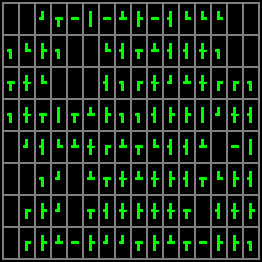
\includegraphics[scale=0.75]{\CURPATH/shuffled.png}
\caption{Разобранная головоломка}
\end{figure}

\dots и собранная:

\begin{figure}[H]
\label{fig:pipe_solved}
\centering
\includegraphics[scale=0.75]{\CURPATH/solved.png}
\caption{Собранная головоломка}
\end{figure}

Попробуем найти способ собрать её.

\subsubsection{Создание}

В начале, нужно её создать.
Вот простая идея.
Возьем массив ячеек 8*16.
Каждая ячейка может содержать какой-то тип блока.
Между ячейками есть стыки:

\input{\CURPATH/pipe_gen.tex}

Синие линии это горизонтальные стыки, красные линии это вертикальные стыки.
Мы просто случайно выставляем каждый стык в 0/false (отсутствует) или 1/true (присутствует).

После этого, теперь легко найти тип каждой ячейки.
А это:

\newcommand{\HeaderColor}{\cellcolor{blue!25}}
\begin{center}
\begin{longtable}{ | l | l | l | l | }
\hline
\HeaderColor стыки & \HeaderColor наше внутреннее название & \HeaderColor угол & \HeaderColor символ \\
\hline
0	&type 0		&	0$^{\circ}$	& (пробел)	\\
2	&type 2a	&	0$^{\circ}$	& \pmboxdrawuni{2503} \\ % ┃
2	&type 2a	&	90$^{\circ}$	& \pmboxdrawuni{2501} \\ % ━
2	&type 2b	&	0$^{\circ}$	& \pmboxdrawuni{250F} \\ % ┏
2	&type 2b	&	90$^{\circ}$	& \pmboxdrawuni{2513} \\ % ┓
2	&type 2b	&	180$^{\circ}$	& \pmboxdrawuni{251B} \\ % ┛
2	&type 2b	&	270$^{\circ}$	& \pmboxdrawuni{2517} \\ % ┗
3	&type 3		&	0$^{\circ}$	& \pmboxdrawuni{2523} \\ % ┣
3 	&type 3		&	90$^{\circ}$	& \pmboxdrawuni{2533} \\ % ┳
3	&type 3		&	180$^{\circ}$	& \pmboxdrawuni{252B} \\ % ┫
3	&type 3		&	270$^{\circ}$	& \pmboxdrawuni{253B} \\ % ┻
4	&type 4		&	0$^{\circ}$	& \pmboxdrawuni{254B} \\ % ╋
\hline
\end{longtable}
\end{center}

\textit{Висящие} стыки могут присутствовать на первой стадии (т.е., ячейки только с одним стыком), но они удалются
рекурсивно, и эти ячейки преобразуются в пустые ячейки.
Так что, в самом конце, все ячейки имеют минимум 2 стыка, и вся эта сантехническая система не имеет связей с внешним миром ---
я надеюсь, из-за этого станет немного проще.

Исходник генератора на Си здесь: \url{.../pipe/generator}.
Все вертикальные стыки хранятся в глобальном массиве \textit{hjoints[]} и вертикальные в \textit{vjoints[]}.

Программа на Си генерирует ANSI-раскрашенный вывод, как это было показано выше
(\ref{fig:pipe_shuffled}, \ref{fig:pipe_solved}) плюс массив типов для каждой ячейки, но без информации об углах:

\begin{lstlisting}[label=init_cells]
[
["0", "0", "2b", "3", "2a", "2a", "2a", "3", "3", "2a", "3", "2b", "2b", "2b", "0", "0"],
["2b", "2b", "3", "2b", "0", "0", "2b", "3", "3", "3", "3", "3", "4", "2b", "0", "0"],
["3", "4", "2b", "0", "0", "0", "3", "2b", "2b", "4", "2b", "3", "4", "2b", "2b", "2b"],
["2b", "4", "3", "2a", "3", "3", "3", "2b", "2b", "3", "3", "3", "2a", "2b", "4", "3"],
["0", "2b", "3", "2b", "3", "4", "2b", "3", "3", "2b", "3", "3", "3", "0", "2a", "2a"],
["0", "0", "2b", "2b", "0", "3", "3", "4", "3", "4", "3", "3", "3", "2b", "3", "3"],
["0", "2b", "3", "2b", "0", "3", "3", "4", "3", "4", "4", "3", "0", "3", "4", "3"],
["0", "2b", "3", "3", "2a", "3", "2b", "2b", "3", "3", "3", "3", "2a", "3", "3", "2b"],
]
\end{lstlisting}

\subsubsection{Решение}

Прежде всего, мы будем работать с массивом ячеек 8*16, где каждый элемент имеет 4 бита:
``T'' (top/верх),
``B'' (bottom/низ),
``L'' (left/лево),
``R'' (right/право).
Каждый бит представляет собой половину стыка.

\input{\CURPATH/pipe_solve.tex}

Теперь определяем массив для каждого из четырех полустыков + информация об угле:

\begin{lstlisting}
HEIGHT=8
WIDTH=16

# if T/B/R/L is Bool instead of Int, Z3 solver will work faster
T=[[Bool('cell_%d_%d_top' % (r, c)) for c in range(WIDTH)] for r in range(HEIGHT)]
B=[[Bool('cell_%d_%d_bottom' % (r, c)) for c in range(WIDTH)] for r in range(HEIGHT)]
R=[[Bool('cell_%d_%d_right' % (r, c)) for c in range(WIDTH)] for r in range(HEIGHT)]
L=[[Bool('cell_%d_%d_left' % (r, c)) for c in range(WIDTH)] for r in range(HEIGHT)]
A=[[Int('cell_%d_%d_angle' % (r, c)) for c in range(WIDTH)] for r in range(HEIGHT)]
\end{lstlisting}

Мы знаем, что если каждый из полустыков присутствует, ответный полустык также должен присутствовать, и наоборот. 
Определяем всё это используя эти констрайнты:

\begin{lstlisting}
# shorthand variables for True and False:
t=True
f=False

# "top" of each cell must be equal to "bottom" of the cell above
# "bottom" of each cell must be equal to "top" of the cell below
# "left" of each cell must be equal to "right" of the cell at left
# "right" of each cell must be equal to "left" of the cell at right
for r in range(HEIGHT):
    for c in range(WIDTH):
        if r!=0:
            s.add(T[r][c]==B[r-1][c])
        if r!=HEIGHT-1:
            s.add(B[r][c]==T[r+1][c])
        if c!=0:
            s.add(L[r][c]==R[r][c-1])
        if c!=WIDTH-1:
            s.add(R[r][c]==L[r][c+1])

# "left" of each cell of first column shouldn't have any connection
# so is "right" of each cell of the last column
for r in range(HEIGHT):
    s.add(L[r][0]==f)
    s.add(R[r][WIDTH-1]==f)

# "top" of each cell of the first row shouldn't have any connection
# so is "bottom" of each cell of the last row
for c in range(WIDTH):
    s.add(T[0][c]==f)
    s.add(B[HEIGHT-1][c]==f)
\end{lstlisting}

Теперь перебираем все ячейки в изначальном массиве (\ref{init_cells}).
Первые две ячейки здесь пустые. И третья имеет тип ``2b''.
Это ``\pmboxdrawuni{250F}'' % ┏
и его можно ориентировать четырьмя разными способами.
И если её угол это 0$^{\circ}$, верхний и правый полустыки присутствуют, остальные отсутствуют.
Если он имеет угол 90$^{\circ}$, он выглядит как 
``\pmboxdrawuni{2513}'', % ┓
и верхник и левый полустыки присутствуют, остальные отсутствуют.

На обычном русском языке: ``если ячейка этого типа имеет угол 0$^{\circ}$, вот эти полустыки должны присутствовать \textbf{ИЛИ}
если она имеет угол 90$^{\circ}$, эти полустыки должны присутствовать, \textbf{ИЛИ}, итд, итд.''

Точно также, мы определяем эти правила для всех типов и всех возможных углов:

\begin{lstlisting}
for r in range(HEIGHT):
    for c in range(WIDTH):
        ty=cells_type[r][c]

        if ty=="0":
            s.add(A[r][c]==f)
            s.add(T[r][c]==f, B[r][c]==f, L[r][c]==f, R[r][c]==f)

        if ty=="2a":
            s.add(Or(And(A[r][c]==0, L[r][c]==f, R[r][c]==f, T[r][c]==t, B[r][c]==t),   # §\pmboxdrawuni{2503}§
                    And(A[r][c]==90, L[r][c]==t, R[r][c]==t, T[r][c]==f, B[r][c]==f)))  # §\pmboxdrawuni{2501}§

        if ty=="2b":
            s.add(Or(And(A[r][c]==0, L[r][c]==f, R[r][c]==t, T[r][c]==f, B[r][c]==t),   # §\pmboxdrawuni{250F}§
                    And(A[r][c]==90, L[r][c]==t, R[r][c]==f, T[r][c]==f, B[r][c]==t),   # §\pmboxdrawuni{2513}§
                    And(A[r][c]==180, L[r][c]==t, R[r][c]==f, T[r][c]==t, B[r][c]==f),  # §\pmboxdrawuni{251B}§
                    And(A[r][c]==270, L[r][c]==f, R[r][c]==t, T[r][c]==t, B[r][c]==f))) # §\pmboxdrawuni{2517}§
	
        if ty=="3":
            s.add(Or(And(A[r][c]==0, L[r][c]==f, R[r][c]==t, T[r][c]==t, B[r][c]==t),   # §\pmboxdrawuni{2523}§
                    And(A[r][c]==90, L[r][c]==t, R[r][c]==t, T[r][c]==f, B[r][c]==t),   # §\pmboxdrawuni{2533}§
                    And(A[r][c]==180, L[r][c]==t, R[r][c]==f, T[r][c]==t, B[r][c]==t),  # §\pmboxdrawuni{252B}§
                    And(A[r][c]==270, L[r][c]==t, R[r][c]==t, T[r][c]==t, B[r][c]==f))) # §\pmboxdrawuni{253B}§

        if ty=="4":
            s.add(A[r][c]==0)
            s.add(T[r][c]==t, B[r][c]==t, L[r][c]==t, R[r][c]==t) # §\pmboxdrawuni{254B}§
\end{lstlisting}

Полный исходник здесь: \url{.../solver/solve_pipe_puzzle1.py}.

Получается такой результат (выводит угол для каждой ячейки и (псевдо)графическое представление):

\begin{figure}[H]
\centering
\includegraphics[scale=0.75]{\CURPATH/solver/solver.png}
\caption{Вывод скрипта солвера}
\end{figure}

Это работает $\approx 4$ секунды на моем старом и медленном Intel Atom N455 1.66GHz.
Быстро ли это? Не знаю, но снова вот что действительно круто, это то что мы понятия не имеем о какой-то математической
теории за всем этим, мы просто объявили ячейки, (полу-)стыки и определили отношения между ними.

Теперь следующий вопрос это, сколько здесь возможных решений?
Используя раннее описанный метод (\ref{SMTEnumerate}), я немного изменил скрипт солвера
\footnote{\url{.../solver/solve_pipe_puzzle2.py}} и солвер
сказал что возможно два решения.

Сравним их используя gvimdiff:

\begin{figure}[H]
\centering
\includegraphics[scale=0.75]{\CURPATH/solver/diff.png}
\caption{Вывод gvimdiff (извините за мой красный курсор в левой части в левом верхнем углу)}
\end{figure}

4 ячейки в середине могут быть ориентированы по-разному.
Видимо, другие головоломки могут также выдавать разные результаты.

P.S.
\textit{Полу-стык} определен как булевый тип.
Но на самом деле, первая версия солвера была написана используя целочисленный тип для полу-стыков,
и 0 использовалось для False и 1 для True.
Я так сделал, потому что хотел более компактный исходный код, без использования длинных слов как ``False'' и ``True''.
И это работало, но медленнее. Вероятно, Z3 работает с булевыми типами быстрее? Лучше?
Так или иначе, я пишу это чтобы отметить, что, если нужно, целочисленный тип можно использовать вместо булевого.


\section{Развлекательная математика и головоломки}

\input{puzzles/sudoku/main_RU}
\input{puzzles/zebra/main_RU}
\input{puzzles/pipe/main_RU}
\input{puzzles/rubik2/failed_SMT/main_RU}
\input{puzzles/rubik2/SAT/main_RU}
\input{puzzles/rubik3/one_face_SMT/main_RU}
%\input{puzzles/numberlink/main_RU}
%\input{puzzles/two_parks_RU}
\input{puzzles/alphametics/main_RU}
%\input{puzzles/2015_AIME_II_Problems_12_RU}
%\input{puzzles/fred/main_RU}
%\input{puzzles/MC/main_RU}
%\input{puzzles/coin_flip/main_RU}
%\input{puzzles/Mock_AIME_2_2006-2007_Problem_8_RU}
%\input{puzzles/2012_AIME_I_Problems_1_RU}
%\input{puzzles/keypad_RU}


\section{Развлекательная математика и головоломки}

\input{puzzles/sudoku/main_RU}
\input{puzzles/zebra/main_RU}
\input{puzzles/pipe/main_RU}
\input{puzzles/rubik2/failed_SMT/main_RU}
\input{puzzles/rubik2/SAT/main_RU}
\input{puzzles/rubik3/one_face_SMT/main_RU}
%\input{puzzles/numberlink/main_RU}
%\input{puzzles/two_parks_RU}
\input{puzzles/alphametics/main_RU}
%\input{puzzles/2015_AIME_II_Problems_12_RU}
%\input{puzzles/fred/main_RU}
%\input{puzzles/MC/main_RU}
%\input{puzzles/coin_flip/main_RU}
%\input{puzzles/Mock_AIME_2_2006-2007_Problem_8_RU}
%\input{puzzles/2012_AIME_I_Problems_1_RU}
%\input{puzzles/keypad_RU}


\section{Развлекательная математика и головоломки}

\input{puzzles/sudoku/main_RU}
\input{puzzles/zebra/main_RU}
\input{puzzles/pipe/main_RU}
\input{puzzles/rubik2/failed_SMT/main_RU}
\input{puzzles/rubik2/SAT/main_RU}
\input{puzzles/rubik3/one_face_SMT/main_RU}
%\input{puzzles/numberlink/main_RU}
%\input{puzzles/two_parks_RU}
\input{puzzles/alphametics/main_RU}
%\input{puzzles/2015_AIME_II_Problems_12_RU}
%\input{puzzles/fred/main_RU}
%\input{puzzles/MC/main_RU}
%\input{puzzles/coin_flip/main_RU}
%\input{puzzles/Mock_AIME_2_2006-2007_Problem_8_RU}
%\input{puzzles/2012_AIME_I_Problems_1_RU}
%\input{puzzles/keypad_RU}


%\section{Развлекательная математика и головоломки}

\input{puzzles/sudoku/main_RU}
\input{puzzles/zebra/main_RU}
\input{puzzles/pipe/main_RU}
\input{puzzles/rubik2/failed_SMT/main_RU}
\input{puzzles/rubik2/SAT/main_RU}
\input{puzzles/rubik3/one_face_SMT/main_RU}
%\input{puzzles/numberlink/main_RU}
%\input{puzzles/two_parks_RU}
\input{puzzles/alphametics/main_RU}
%\input{puzzles/2015_AIME_II_Problems_12_RU}
%\input{puzzles/fred/main_RU}
%\input{puzzles/MC/main_RU}
%\input{puzzles/coin_flip/main_RU}
%\input{puzzles/Mock_AIME_2_2006-2007_Problem_8_RU}
%\input{puzzles/2012_AIME_I_Problems_1_RU}
%\input{puzzles/keypad_RU}


%\input{puzzles/two_parks_RU}
\subsection{Альфаметика}

Согласно Дональду Кнуту, термин ``Альфаметика'' был придуман Дж. Эйч. Аш. Хантером.
Это головоломка: какие десятичные цифры в пределах 0..9 нужно присвоить каждой букве, чтобы это уравнение было справедливо?

\begin{lstlisting}
  SEND
+ MORE
 -----
 MONEY
\end{lstlisting}

Для Z3 это легко:

\lstinputlisting{puzzles/alphametics/alpha.py}

Вывод:

\begin{lstlisting}
sat
[E, = 5,
 S, = 9,
 M, = 1,
 N, = 6,
 D, = 7,
 R, = 8,
 O, = 0,
 Y = 2]
\end{lstlisting}

Вот еще одна, из \ac{TAOCP} том IV (\url{http://www-cs-faculty.stanford.edu/~uno/fasc2b.ps.gz}):

\lstinputlisting{puzzles/alphametics/alpha2.py}

\begin{lstlisting}
sat
[L, = 6,
 S, = 7,
 N, = 2,
 T, = 1,
 I, = 5,
 V = 3,
 A, = 8,
 R, = 9,
 O, = 4,
 TRIO = 1954,
 SONATA, = 742818,
 VIOLA, = 35468,
 VIOLIN, = 354652]
\end{lstlisting}

% TODO URL
Эту головоломку я нашел в примерах pySMT:

\lstinputlisting{puzzles/alphametics/alpha3.py}

\begin{lstlisting}
sat
[D = 5, R = 4, O = 3, E = 8, L = 6, W = 7, H = 2]
\end{lstlisting}

%%% 

Это упражнение Q209 из
[Companion to the Papers of Donald Knuth]\footnote{\url{http://www-cs-faculty.stanford.edu/~knuth/cp.html}}.

\begin{lstlisting}
 KNIFE
  FORK
 SPOON
  SOUP
------
SUPPER
\end{lstlisting}

В целях упрощения, я добавил ф-цию (list\_to\_expr()):

\lstinputlisting{puzzles/alphametics/alpha4.py}

\begin{lstlisting}
sat
[K = 7,
 N = 4,
 R = 9,
 I = 1,
 E = 6,
 S = 0,
 O = 3,
 F = 5,
 U = 8,
 P = 2,
 SUPPER = 82269,
 SOUP = 382,
 SPOON = 2334,
 FORK = 5397,
 KNIFE = 74156]
\end{lstlisting}

S это 0, так что значение SUPPER начинается с (убранного) нуля. Скажем так, нам это не нравится.
Добавим это, чтобы это исправить:

\begin{lstlisting}
s.add(S!=0)
\end{lstlisting}

\begin{lstlisting}
sat
[K = 8,
 N = 4,
 R = 3,
 I = 7,
 E = 6,
 S = 1,
 O = 9,
 F = 2,
 U = 0,
 P = 5,
 SUPPER = 105563,
 SOUP = 1905,
 SPOON = 15994,
 FORK = 2938,
 KNIFE = 84726]
\end{lstlisting}

\paragraph{Создание своей собственной головоломки}

Вот проблема: есть только 10 букв, но как их выбрать из числа слов?
Мы можем использовать Z3 для этого:

\lstinputlisting{puzzles/alphametics/gen.py}

Это первая сгенерированная головоломка:

\begin{lstlisting}
sat
EGGS
JELLY
LUNCH
C 5
E 6
G 3
H 7
J 0
L 1
N 4
S 8
U 2
Y 9
\end{lstlisting}

Что если мы хотим, чтобы слово ``CAKE'' присутствовало в числе ``слагаемых''?

Добавим это:

\begin{lstlisting}
s.add(word_used[words.index('CAKE')])
\end{lstlisting}

\begin{lstlisting}
sat
CAKE
TEA
LUNCH
A 8
C 3
E 1
H 9
J 6
K 2
L 0
N 5
T 7
U 4
\end{lstlisting}

Добавим это:

\begin{lstlisting}
s.add(word_used[words.index('EGGS')])
\end{lstlisting}

Теперь оно может найти пару к EGGS:

\begin{lstlisting}
sat
EGGS
HONEY
LUNCH
C 6
E 7
G 9
H 4
L 5
N 8
O 2
S 3
U 0
Y 1
\end{lstlisting}

\paragraph{Файлы}

\url{https://github.com/DennisYurichev/...}




%\input{puzzles/2015_AIME_II_Problems_12_RU}
%\section{Развлекательная математика и головоломки}

\input{puzzles/sudoku/main_RU}
\input{puzzles/zebra/main_RU}
\input{puzzles/pipe/main_RU}
\input{puzzles/rubik2/failed_SMT/main_RU}
\input{puzzles/rubik2/SAT/main_RU}
\input{puzzles/rubik3/one_face_SMT/main_RU}
%\input{puzzles/numberlink/main_RU}
%\input{puzzles/two_parks_RU}
\input{puzzles/alphametics/main_RU}
%\input{puzzles/2015_AIME_II_Problems_12_RU}
%\input{puzzles/fred/main_RU}
%\input{puzzles/MC/main_RU}
%\input{puzzles/coin_flip/main_RU}
%\input{puzzles/Mock_AIME_2_2006-2007_Problem_8_RU}
%\input{puzzles/2012_AIME_I_Problems_1_RU}
%\input{puzzles/keypad_RU}


%\section{Развлекательная математика и головоломки}

\input{puzzles/sudoku/main_RU}
\input{puzzles/zebra/main_RU}
\input{puzzles/pipe/main_RU}
\input{puzzles/rubik2/failed_SMT/main_RU}
\input{puzzles/rubik2/SAT/main_RU}
\input{puzzles/rubik3/one_face_SMT/main_RU}
%\input{puzzles/numberlink/main_RU}
%\input{puzzles/two_parks_RU}
\input{puzzles/alphametics/main_RU}
%\input{puzzles/2015_AIME_II_Problems_12_RU}
%\input{puzzles/fred/main_RU}
%\input{puzzles/MC/main_RU}
%\input{puzzles/coin_flip/main_RU}
%\input{puzzles/Mock_AIME_2_2006-2007_Problem_8_RU}
%\input{puzzles/2012_AIME_I_Problems_1_RU}
%\input{puzzles/keypad_RU}


%\section{Развлекательная математика и головоломки}

\input{puzzles/sudoku/main_RU}
\input{puzzles/zebra/main_RU}
\input{puzzles/pipe/main_RU}
\input{puzzles/rubik2/failed_SMT/main_RU}
\input{puzzles/rubik2/SAT/main_RU}
\input{puzzles/rubik3/one_face_SMT/main_RU}
%\input{puzzles/numberlink/main_RU}
%\input{puzzles/two_parks_RU}
\input{puzzles/alphametics/main_RU}
%\input{puzzles/2015_AIME_II_Problems_12_RU}
%\input{puzzles/fred/main_RU}
%\input{puzzles/MC/main_RU}
%\input{puzzles/coin_flip/main_RU}
%\input{puzzles/Mock_AIME_2_2006-2007_Problem_8_RU}
%\input{puzzles/2012_AIME_I_Problems_1_RU}
%\input{puzzles/keypad_RU}


%\input{puzzles/Mock_AIME_2_2006-2007_Problem_8_RU}
%\input{puzzles/2012_AIME_I_Problems_1_RU}
%\input{puzzles/keypad_RU}


%\input{puzzles/two_parks_RU}
\subsection{Альфаметика}

Согласно Дональду Кнуту, термин ``Альфаметика'' был придуман Дж. Эйч. Аш. Хантером.
Это головоломка: какие десятичные цифры в пределах 0..9 нужно присвоить каждой букве, чтобы это уравнение было справедливо?

\begin{lstlisting}
  SEND
+ MORE
 -----
 MONEY
\end{lstlisting}

Для Z3 это легко:

\lstinputlisting{puzzles/alphametics/alpha.py}

Вывод:

\begin{lstlisting}
sat
[E, = 5,
 S, = 9,
 M, = 1,
 N, = 6,
 D, = 7,
 R, = 8,
 O, = 0,
 Y = 2]
\end{lstlisting}

Вот еще одна, из \ac{TAOCP} том IV (\url{http://www-cs-faculty.stanford.edu/~uno/fasc2b.ps.gz}):

\lstinputlisting{puzzles/alphametics/alpha2.py}

\begin{lstlisting}
sat
[L, = 6,
 S, = 7,
 N, = 2,
 T, = 1,
 I, = 5,
 V = 3,
 A, = 8,
 R, = 9,
 O, = 4,
 TRIO = 1954,
 SONATA, = 742818,
 VIOLA, = 35468,
 VIOLIN, = 354652]
\end{lstlisting}

% TODO URL
Эту головоломку я нашел в примерах pySMT:

\lstinputlisting{puzzles/alphametics/alpha3.py}

\begin{lstlisting}
sat
[D = 5, R = 4, O = 3, E = 8, L = 6, W = 7, H = 2]
\end{lstlisting}

%%% 

Это упражнение Q209 из
[Companion to the Papers of Donald Knuth]\footnote{\url{http://www-cs-faculty.stanford.edu/~knuth/cp.html}}.

\begin{lstlisting}
 KNIFE
  FORK
 SPOON
  SOUP
------
SUPPER
\end{lstlisting}

В целях упрощения, я добавил ф-цию (list\_to\_expr()):

\lstinputlisting{puzzles/alphametics/alpha4.py}

\begin{lstlisting}
sat
[K = 7,
 N = 4,
 R = 9,
 I = 1,
 E = 6,
 S = 0,
 O = 3,
 F = 5,
 U = 8,
 P = 2,
 SUPPER = 82269,
 SOUP = 382,
 SPOON = 2334,
 FORK = 5397,
 KNIFE = 74156]
\end{lstlisting}

S это 0, так что значение SUPPER начинается с (убранного) нуля. Скажем так, нам это не нравится.
Добавим это, чтобы это исправить:

\begin{lstlisting}
s.add(S!=0)
\end{lstlisting}

\begin{lstlisting}
sat
[K = 8,
 N = 4,
 R = 3,
 I = 7,
 E = 6,
 S = 1,
 O = 9,
 F = 2,
 U = 0,
 P = 5,
 SUPPER = 105563,
 SOUP = 1905,
 SPOON = 15994,
 FORK = 2938,
 KNIFE = 84726]
\end{lstlisting}

\paragraph{Создание своей собственной головоломки}

Вот проблема: есть только 10 букв, но как их выбрать из числа слов?
Мы можем использовать Z3 для этого:

\lstinputlisting{puzzles/alphametics/gen.py}

Это первая сгенерированная головоломка:

\begin{lstlisting}
sat
EGGS
JELLY
LUNCH
C 5
E 6
G 3
H 7
J 0
L 1
N 4
S 8
U 2
Y 9
\end{lstlisting}

Что если мы хотим, чтобы слово ``CAKE'' присутствовало в числе ``слагаемых''?

Добавим это:

\begin{lstlisting}
s.add(word_used[words.index('CAKE')])
\end{lstlisting}

\begin{lstlisting}
sat
CAKE
TEA
LUNCH
A 8
C 3
E 1
H 9
J 6
K 2
L 0
N 5
T 7
U 4
\end{lstlisting}

Добавим это:

\begin{lstlisting}
s.add(word_used[words.index('EGGS')])
\end{lstlisting}

Теперь оно может найти пару к EGGS:

\begin{lstlisting}
sat
EGGS
HONEY
LUNCH
C 6
E 7
G 9
H 4
L 5
N 8
O 2
S 3
U 0
Y 1
\end{lstlisting}

\paragraph{Файлы}

\url{https://github.com/DennisYurichev/...}




%\input{puzzles/2015_AIME_II_Problems_12_RU}
%\section{Развлекательная математика и головоломки}

\subsection{Судоку}

Головоломка Судоку это решетка 9*9, некоторые ячейки заполнены значениями, некоторые пустые:

% copypasted from http://www.texample.net/tikz/examples/sudoku/
\newcounter{row}
\newcounter{col}

\newcommand\setrow[9]{
  \setcounter{col}{1}
  \foreach \n in {#1, #2, #3, #4, #5, #6, #7, #8, #9} {
    \edef\x{\value{col} - 0.5}
    \edef\y{9.5 - \value{row}}
    \node[anchor=center] at (\x, \y) {\n};
    \stepcounter{col}
  }
  \stepcounter{row}
}

\begin{center}
\begin{tikzpicture}[scale=.7]
  \begin{scope}
    \draw (0, 0) grid (9, 9);
    \draw[very thick, scale=3] (0, 0) grid (3, 3);

    \setcounter{row}{1}
    \setrow { }{ }{5}  {3}{ }{ }  { }{ }{ }
    \setrow {8}{ }{ }  { }{ }{ }  { }{2}{ }
    \setrow { }{7}{ }  { }{1}{ }  {5}{ }{ }

    \setrow {4}{ }{ }  { }{ }{5}  {3}{ }{ }
    \setrow { }{1}{ }  { }{7}{ }  { }{ }{6}
    \setrow { }{ }{3}  {2}{ }{ }  { }{8}{ }

    \setrow { }{6}{ }  {5}{ }{ }  { }{ }{9}
    \setrow { }{ }{4}  { }{ }{ }  { }{3}{ }
    \setrow { }{ }{ }  { }{ }{9}  {7}{ }{ }

    \node[anchor=center] at (4.5, -0.5) {Нерешенная Судоку};
  \end{scope}
\end{tikzpicture}
\end{center}

Числа в каждом ряду должны быть уникальными, т.е., каждый ряд должен содержать 9 чисел в пределах 1..9 без повторений.
Та же история и для каждого столбца и каждого квадрата 3*3.

Головоломка представляет собой хороший кандидат, на котором можно попробовать \ac{SMT}-солвер, потому что это,
в общем-то, просто нерешенная система уравнений.

\input{puzzles/sudoku/1/main_RU}
%\input{puzzles/sudoku/GT/main_RU}
%\input{puzzles/sudoku/killer/main_RU}
\input{puzzles/sudoku/KLEE/main_RU}
\input{puzzles/sudoku/SAT/main_RU}


\subsection{Головоломка зебры (\ac{AKA} Загадка Эйнштейна)}

\input{puzzles/zebra/SMT/main_RU}
\input{puzzles/zebra/KLEE/main_RU}
\input{puzzles/zebra/SAT/main_RU}


\subsection{Решение головоломки ``трубы'' используя Z3 SMT-солвер}

\renewcommand{\CURPATH}{puzzles/pipe}

Головоломка ``трубы'' это популярная головоломка (просто погуглите ``pipe puzzle'' и посмотрите на картинки).

Вот как выглядит головоломка в разобранном виде:

\begin{figure}[H]
\label{fig:pipe_shuffled}
\centering
\includegraphics[scale=0.75]{\CURPATH/shuffled.png}
\caption{Разобранная головоломка}
\end{figure}

\dots и собранная:

\begin{figure}[H]
\label{fig:pipe_solved}
\centering
\includegraphics[scale=0.75]{\CURPATH/solved.png}
\caption{Собранная головоломка}
\end{figure}

Попробуем найти способ собрать её.

\subsubsection{Создание}

В начале, нужно её создать.
Вот простая идея.
Возьем массив ячеек 8*16.
Каждая ячейка может содержать какой-то тип блока.
Между ячейками есть стыки:

\input{\CURPATH/pipe_gen.tex}

Синие линии это горизонтальные стыки, красные линии это вертикальные стыки.
Мы просто случайно выставляем каждый стык в 0/false (отсутствует) или 1/true (присутствует).

После этого, теперь легко найти тип каждой ячейки.
А это:

\newcommand{\HeaderColor}{\cellcolor{blue!25}}
\begin{center}
\begin{longtable}{ | l | l | l | l | }
\hline
\HeaderColor стыки & \HeaderColor наше внутреннее название & \HeaderColor угол & \HeaderColor символ \\
\hline
0	&type 0		&	0$^{\circ}$	& (пробел)	\\
2	&type 2a	&	0$^{\circ}$	& \pmboxdrawuni{2503} \\ % ┃
2	&type 2a	&	90$^{\circ}$	& \pmboxdrawuni{2501} \\ % ━
2	&type 2b	&	0$^{\circ}$	& \pmboxdrawuni{250F} \\ % ┏
2	&type 2b	&	90$^{\circ}$	& \pmboxdrawuni{2513} \\ % ┓
2	&type 2b	&	180$^{\circ}$	& \pmboxdrawuni{251B} \\ % ┛
2	&type 2b	&	270$^{\circ}$	& \pmboxdrawuni{2517} \\ % ┗
3	&type 3		&	0$^{\circ}$	& \pmboxdrawuni{2523} \\ % ┣
3 	&type 3		&	90$^{\circ}$	& \pmboxdrawuni{2533} \\ % ┳
3	&type 3		&	180$^{\circ}$	& \pmboxdrawuni{252B} \\ % ┫
3	&type 3		&	270$^{\circ}$	& \pmboxdrawuni{253B} \\ % ┻
4	&type 4		&	0$^{\circ}$	& \pmboxdrawuni{254B} \\ % ╋
\hline
\end{longtable}
\end{center}

\textit{Висящие} стыки могут присутствовать на первой стадии (т.е., ячейки только с одним стыком), но они удалются
рекурсивно, и эти ячейки преобразуются в пустые ячейки.
Так что, в самом конце, все ячейки имеют минимум 2 стыка, и вся эта сантехническая система не имеет связей с внешним миром ---
я надеюсь, из-за этого станет немного проще.

Исходник генератора на Си здесь: \url{.../pipe/generator}.
Все вертикальные стыки хранятся в глобальном массиве \textit{hjoints[]} и вертикальные в \textit{vjoints[]}.

Программа на Си генерирует ANSI-раскрашенный вывод, как это было показано выше
(\ref{fig:pipe_shuffled}, \ref{fig:pipe_solved}) плюс массив типов для каждой ячейки, но без информации об углах:

\begin{lstlisting}[label=init_cells]
[
["0", "0", "2b", "3", "2a", "2a", "2a", "3", "3", "2a", "3", "2b", "2b", "2b", "0", "0"],
["2b", "2b", "3", "2b", "0", "0", "2b", "3", "3", "3", "3", "3", "4", "2b", "0", "0"],
["3", "4", "2b", "0", "0", "0", "3", "2b", "2b", "4", "2b", "3", "4", "2b", "2b", "2b"],
["2b", "4", "3", "2a", "3", "3", "3", "2b", "2b", "3", "3", "3", "2a", "2b", "4", "3"],
["0", "2b", "3", "2b", "3", "4", "2b", "3", "3", "2b", "3", "3", "3", "0", "2a", "2a"],
["0", "0", "2b", "2b", "0", "3", "3", "4", "3", "4", "3", "3", "3", "2b", "3", "3"],
["0", "2b", "3", "2b", "0", "3", "3", "4", "3", "4", "4", "3", "0", "3", "4", "3"],
["0", "2b", "3", "3", "2a", "3", "2b", "2b", "3", "3", "3", "3", "2a", "3", "3", "2b"],
]
\end{lstlisting}

\subsubsection{Решение}

Прежде всего, мы будем работать с массивом ячеек 8*16, где каждый элемент имеет 4 бита:
``T'' (top/верх),
``B'' (bottom/низ),
``L'' (left/лево),
``R'' (right/право).
Каждый бит представляет собой половину стыка.

\input{\CURPATH/pipe_solve.tex}

Теперь определяем массив для каждого из четырех полустыков + информация об угле:

\begin{lstlisting}
HEIGHT=8
WIDTH=16

# if T/B/R/L is Bool instead of Int, Z3 solver will work faster
T=[[Bool('cell_%d_%d_top' % (r, c)) for c in range(WIDTH)] for r in range(HEIGHT)]
B=[[Bool('cell_%d_%d_bottom' % (r, c)) for c in range(WIDTH)] for r in range(HEIGHT)]
R=[[Bool('cell_%d_%d_right' % (r, c)) for c in range(WIDTH)] for r in range(HEIGHT)]
L=[[Bool('cell_%d_%d_left' % (r, c)) for c in range(WIDTH)] for r in range(HEIGHT)]
A=[[Int('cell_%d_%d_angle' % (r, c)) for c in range(WIDTH)] for r in range(HEIGHT)]
\end{lstlisting}

Мы знаем, что если каждый из полустыков присутствует, ответный полустык также должен присутствовать, и наоборот. 
Определяем всё это используя эти констрайнты:

\begin{lstlisting}
# shorthand variables for True and False:
t=True
f=False

# "top" of each cell must be equal to "bottom" of the cell above
# "bottom" of each cell must be equal to "top" of the cell below
# "left" of each cell must be equal to "right" of the cell at left
# "right" of each cell must be equal to "left" of the cell at right
for r in range(HEIGHT):
    for c in range(WIDTH):
        if r!=0:
            s.add(T[r][c]==B[r-1][c])
        if r!=HEIGHT-1:
            s.add(B[r][c]==T[r+1][c])
        if c!=0:
            s.add(L[r][c]==R[r][c-1])
        if c!=WIDTH-1:
            s.add(R[r][c]==L[r][c+1])

# "left" of each cell of first column shouldn't have any connection
# so is "right" of each cell of the last column
for r in range(HEIGHT):
    s.add(L[r][0]==f)
    s.add(R[r][WIDTH-1]==f)

# "top" of each cell of the first row shouldn't have any connection
# so is "bottom" of each cell of the last row
for c in range(WIDTH):
    s.add(T[0][c]==f)
    s.add(B[HEIGHT-1][c]==f)
\end{lstlisting}

Теперь перебираем все ячейки в изначальном массиве (\ref{init_cells}).
Первые две ячейки здесь пустые. И третья имеет тип ``2b''.
Это ``\pmboxdrawuni{250F}'' % ┏
и его можно ориентировать четырьмя разными способами.
И если её угол это 0$^{\circ}$, верхний и правый полустыки присутствуют, остальные отсутствуют.
Если он имеет угол 90$^{\circ}$, он выглядит как 
``\pmboxdrawuni{2513}'', % ┓
и верхник и левый полустыки присутствуют, остальные отсутствуют.

На обычном русском языке: ``если ячейка этого типа имеет угол 0$^{\circ}$, вот эти полустыки должны присутствовать \textbf{ИЛИ}
если она имеет угол 90$^{\circ}$, эти полустыки должны присутствовать, \textbf{ИЛИ}, итд, итд.''

Точно также, мы определяем эти правила для всех типов и всех возможных углов:

\begin{lstlisting}
for r in range(HEIGHT):
    for c in range(WIDTH):
        ty=cells_type[r][c]

        if ty=="0":
            s.add(A[r][c]==f)
            s.add(T[r][c]==f, B[r][c]==f, L[r][c]==f, R[r][c]==f)

        if ty=="2a":
            s.add(Or(And(A[r][c]==0, L[r][c]==f, R[r][c]==f, T[r][c]==t, B[r][c]==t),   # §\pmboxdrawuni{2503}§
                    And(A[r][c]==90, L[r][c]==t, R[r][c]==t, T[r][c]==f, B[r][c]==f)))  # §\pmboxdrawuni{2501}§

        if ty=="2b":
            s.add(Or(And(A[r][c]==0, L[r][c]==f, R[r][c]==t, T[r][c]==f, B[r][c]==t),   # §\pmboxdrawuni{250F}§
                    And(A[r][c]==90, L[r][c]==t, R[r][c]==f, T[r][c]==f, B[r][c]==t),   # §\pmboxdrawuni{2513}§
                    And(A[r][c]==180, L[r][c]==t, R[r][c]==f, T[r][c]==t, B[r][c]==f),  # §\pmboxdrawuni{251B}§
                    And(A[r][c]==270, L[r][c]==f, R[r][c]==t, T[r][c]==t, B[r][c]==f))) # §\pmboxdrawuni{2517}§
	
        if ty=="3":
            s.add(Or(And(A[r][c]==0, L[r][c]==f, R[r][c]==t, T[r][c]==t, B[r][c]==t),   # §\pmboxdrawuni{2523}§
                    And(A[r][c]==90, L[r][c]==t, R[r][c]==t, T[r][c]==f, B[r][c]==t),   # §\pmboxdrawuni{2533}§
                    And(A[r][c]==180, L[r][c]==t, R[r][c]==f, T[r][c]==t, B[r][c]==t),  # §\pmboxdrawuni{252B}§
                    And(A[r][c]==270, L[r][c]==t, R[r][c]==t, T[r][c]==t, B[r][c]==f))) # §\pmboxdrawuni{253B}§

        if ty=="4":
            s.add(A[r][c]==0)
            s.add(T[r][c]==t, B[r][c]==t, L[r][c]==t, R[r][c]==t) # §\pmboxdrawuni{254B}§
\end{lstlisting}

Полный исходник здесь: \url{.../solver/solve_pipe_puzzle1.py}.

Получается такой результат (выводит угол для каждой ячейки и (псевдо)графическое представление):

\begin{figure}[H]
\centering
\includegraphics[scale=0.75]{\CURPATH/solver/solver.png}
\caption{Вывод скрипта солвера}
\end{figure}

Это работает $\approx 4$ секунды на моем старом и медленном Intel Atom N455 1.66GHz.
Быстро ли это? Не знаю, но снова вот что действительно круто, это то что мы понятия не имеем о какой-то математической
теории за всем этим, мы просто объявили ячейки, (полу-)стыки и определили отношения между ними.

Теперь следующий вопрос это, сколько здесь возможных решений?
Используя раннее описанный метод (\ref{SMTEnumerate}), я немного изменил скрипт солвера
\footnote{\url{.../solver/solve_pipe_puzzle2.py}} и солвер
сказал что возможно два решения.

Сравним их используя gvimdiff:

\begin{figure}[H]
\centering
\includegraphics[scale=0.75]{\CURPATH/solver/diff.png}
\caption{Вывод gvimdiff (извините за мой красный курсор в левой части в левом верхнем углу)}
\end{figure}

4 ячейки в середине могут быть ориентированы по-разному.
Видимо, другие головоломки могут также выдавать разные результаты.

P.S.
\textit{Полу-стык} определен как булевый тип.
Но на самом деле, первая версия солвера была написана используя целочисленный тип для полу-стыков,
и 0 использовалось для False и 1 для True.
Я так сделал, потому что хотел более компактный исходный код, без использования длинных слов как ``False'' и ``True''.
И это работало, но медленнее. Вероятно, Z3 работает с булевыми типами быстрее? Лучше?
Так или иначе, я пишу это чтобы отметить, что, если нужно, целочисленный тип можно использовать вместо булевого.


\section{Развлекательная математика и головоломки}

\input{puzzles/sudoku/main_RU}
\input{puzzles/zebra/main_RU}
\input{puzzles/pipe/main_RU}
\input{puzzles/rubik2/failed_SMT/main_RU}
\input{puzzles/rubik2/SAT/main_RU}
\input{puzzles/rubik3/one_face_SMT/main_RU}
%\input{puzzles/numberlink/main_RU}
%\input{puzzles/two_parks_RU}
\input{puzzles/alphametics/main_RU}
%\input{puzzles/2015_AIME_II_Problems_12_RU}
%\input{puzzles/fred/main_RU}
%\input{puzzles/MC/main_RU}
%\input{puzzles/coin_flip/main_RU}
%\input{puzzles/Mock_AIME_2_2006-2007_Problem_8_RU}
%\input{puzzles/2012_AIME_I_Problems_1_RU}
%\input{puzzles/keypad_RU}


\section{Развлекательная математика и головоломки}

\input{puzzles/sudoku/main_RU}
\input{puzzles/zebra/main_RU}
\input{puzzles/pipe/main_RU}
\input{puzzles/rubik2/failed_SMT/main_RU}
\input{puzzles/rubik2/SAT/main_RU}
\input{puzzles/rubik3/one_face_SMT/main_RU}
%\input{puzzles/numberlink/main_RU}
%\input{puzzles/two_parks_RU}
\input{puzzles/alphametics/main_RU}
%\input{puzzles/2015_AIME_II_Problems_12_RU}
%\input{puzzles/fred/main_RU}
%\input{puzzles/MC/main_RU}
%\input{puzzles/coin_flip/main_RU}
%\input{puzzles/Mock_AIME_2_2006-2007_Problem_8_RU}
%\input{puzzles/2012_AIME_I_Problems_1_RU}
%\input{puzzles/keypad_RU}


\section{Развлекательная математика и головоломки}

\input{puzzles/sudoku/main_RU}
\input{puzzles/zebra/main_RU}
\input{puzzles/pipe/main_RU}
\input{puzzles/rubik2/failed_SMT/main_RU}
\input{puzzles/rubik2/SAT/main_RU}
\input{puzzles/rubik3/one_face_SMT/main_RU}
%\input{puzzles/numberlink/main_RU}
%\input{puzzles/two_parks_RU}
\input{puzzles/alphametics/main_RU}
%\input{puzzles/2015_AIME_II_Problems_12_RU}
%\input{puzzles/fred/main_RU}
%\input{puzzles/MC/main_RU}
%\input{puzzles/coin_flip/main_RU}
%\input{puzzles/Mock_AIME_2_2006-2007_Problem_8_RU}
%\input{puzzles/2012_AIME_I_Problems_1_RU}
%\input{puzzles/keypad_RU}


%\section{Развлекательная математика и головоломки}

\input{puzzles/sudoku/main_RU}
\input{puzzles/zebra/main_RU}
\input{puzzles/pipe/main_RU}
\input{puzzles/rubik2/failed_SMT/main_RU}
\input{puzzles/rubik2/SAT/main_RU}
\input{puzzles/rubik3/one_face_SMT/main_RU}
%\input{puzzles/numberlink/main_RU}
%\input{puzzles/two_parks_RU}
\input{puzzles/alphametics/main_RU}
%\input{puzzles/2015_AIME_II_Problems_12_RU}
%\input{puzzles/fred/main_RU}
%\input{puzzles/MC/main_RU}
%\input{puzzles/coin_flip/main_RU}
%\input{puzzles/Mock_AIME_2_2006-2007_Problem_8_RU}
%\input{puzzles/2012_AIME_I_Problems_1_RU}
%\input{puzzles/keypad_RU}


%\input{puzzles/two_parks_RU}
\subsection{Альфаметика}

Согласно Дональду Кнуту, термин ``Альфаметика'' был придуман Дж. Эйч. Аш. Хантером.
Это головоломка: какие десятичные цифры в пределах 0..9 нужно присвоить каждой букве, чтобы это уравнение было справедливо?

\begin{lstlisting}
  SEND
+ MORE
 -----
 MONEY
\end{lstlisting}

Для Z3 это легко:

\lstinputlisting{puzzles/alphametics/alpha.py}

Вывод:

\begin{lstlisting}
sat
[E, = 5,
 S, = 9,
 M, = 1,
 N, = 6,
 D, = 7,
 R, = 8,
 O, = 0,
 Y = 2]
\end{lstlisting}

Вот еще одна, из \ac{TAOCP} том IV (\url{http://www-cs-faculty.stanford.edu/~uno/fasc2b.ps.gz}):

\lstinputlisting{puzzles/alphametics/alpha2.py}

\begin{lstlisting}
sat
[L, = 6,
 S, = 7,
 N, = 2,
 T, = 1,
 I, = 5,
 V = 3,
 A, = 8,
 R, = 9,
 O, = 4,
 TRIO = 1954,
 SONATA, = 742818,
 VIOLA, = 35468,
 VIOLIN, = 354652]
\end{lstlisting}

% TODO URL
Эту головоломку я нашел в примерах pySMT:

\lstinputlisting{puzzles/alphametics/alpha3.py}

\begin{lstlisting}
sat
[D = 5, R = 4, O = 3, E = 8, L = 6, W = 7, H = 2]
\end{lstlisting}

%%% 

Это упражнение Q209 из
[Companion to the Papers of Donald Knuth]\footnote{\url{http://www-cs-faculty.stanford.edu/~knuth/cp.html}}.

\begin{lstlisting}
 KNIFE
  FORK
 SPOON
  SOUP
------
SUPPER
\end{lstlisting}

В целях упрощения, я добавил ф-цию (list\_to\_expr()):

\lstinputlisting{puzzles/alphametics/alpha4.py}

\begin{lstlisting}
sat
[K = 7,
 N = 4,
 R = 9,
 I = 1,
 E = 6,
 S = 0,
 O = 3,
 F = 5,
 U = 8,
 P = 2,
 SUPPER = 82269,
 SOUP = 382,
 SPOON = 2334,
 FORK = 5397,
 KNIFE = 74156]
\end{lstlisting}

S это 0, так что значение SUPPER начинается с (убранного) нуля. Скажем так, нам это не нравится.
Добавим это, чтобы это исправить:

\begin{lstlisting}
s.add(S!=0)
\end{lstlisting}

\begin{lstlisting}
sat
[K = 8,
 N = 4,
 R = 3,
 I = 7,
 E = 6,
 S = 1,
 O = 9,
 F = 2,
 U = 0,
 P = 5,
 SUPPER = 105563,
 SOUP = 1905,
 SPOON = 15994,
 FORK = 2938,
 KNIFE = 84726]
\end{lstlisting}

\paragraph{Создание своей собственной головоломки}

Вот проблема: есть только 10 букв, но как их выбрать из числа слов?
Мы можем использовать Z3 для этого:

\lstinputlisting{puzzles/alphametics/gen.py}

Это первая сгенерированная головоломка:

\begin{lstlisting}
sat
EGGS
JELLY
LUNCH
C 5
E 6
G 3
H 7
J 0
L 1
N 4
S 8
U 2
Y 9
\end{lstlisting}

Что если мы хотим, чтобы слово ``CAKE'' присутствовало в числе ``слагаемых''?

Добавим это:

\begin{lstlisting}
s.add(word_used[words.index('CAKE')])
\end{lstlisting}

\begin{lstlisting}
sat
CAKE
TEA
LUNCH
A 8
C 3
E 1
H 9
J 6
K 2
L 0
N 5
T 7
U 4
\end{lstlisting}

Добавим это:

\begin{lstlisting}
s.add(word_used[words.index('EGGS')])
\end{lstlisting}

Теперь оно может найти пару к EGGS:

\begin{lstlisting}
sat
EGGS
HONEY
LUNCH
C 6
E 7
G 9
H 4
L 5
N 8
O 2
S 3
U 0
Y 1
\end{lstlisting}

\paragraph{Файлы}

\url{https://github.com/DennisYurichev/...}




%\input{puzzles/2015_AIME_II_Problems_12_RU}
%\section{Развлекательная математика и головоломки}

\input{puzzles/sudoku/main_RU}
\input{puzzles/zebra/main_RU}
\input{puzzles/pipe/main_RU}
\input{puzzles/rubik2/failed_SMT/main_RU}
\input{puzzles/rubik2/SAT/main_RU}
\input{puzzles/rubik3/one_face_SMT/main_RU}
%\input{puzzles/numberlink/main_RU}
%\input{puzzles/two_parks_RU}
\input{puzzles/alphametics/main_RU}
%\input{puzzles/2015_AIME_II_Problems_12_RU}
%\input{puzzles/fred/main_RU}
%\input{puzzles/MC/main_RU}
%\input{puzzles/coin_flip/main_RU}
%\input{puzzles/Mock_AIME_2_2006-2007_Problem_8_RU}
%\input{puzzles/2012_AIME_I_Problems_1_RU}
%\input{puzzles/keypad_RU}


%\section{Развлекательная математика и головоломки}

\input{puzzles/sudoku/main_RU}
\input{puzzles/zebra/main_RU}
\input{puzzles/pipe/main_RU}
\input{puzzles/rubik2/failed_SMT/main_RU}
\input{puzzles/rubik2/SAT/main_RU}
\input{puzzles/rubik3/one_face_SMT/main_RU}
%\input{puzzles/numberlink/main_RU}
%\input{puzzles/two_parks_RU}
\input{puzzles/alphametics/main_RU}
%\input{puzzles/2015_AIME_II_Problems_12_RU}
%\input{puzzles/fred/main_RU}
%\input{puzzles/MC/main_RU}
%\input{puzzles/coin_flip/main_RU}
%\input{puzzles/Mock_AIME_2_2006-2007_Problem_8_RU}
%\input{puzzles/2012_AIME_I_Problems_1_RU}
%\input{puzzles/keypad_RU}


%\section{Развлекательная математика и головоломки}

\input{puzzles/sudoku/main_RU}
\input{puzzles/zebra/main_RU}
\input{puzzles/pipe/main_RU}
\input{puzzles/rubik2/failed_SMT/main_RU}
\input{puzzles/rubik2/SAT/main_RU}
\input{puzzles/rubik3/one_face_SMT/main_RU}
%\input{puzzles/numberlink/main_RU}
%\input{puzzles/two_parks_RU}
\input{puzzles/alphametics/main_RU}
%\input{puzzles/2015_AIME_II_Problems_12_RU}
%\input{puzzles/fred/main_RU}
%\input{puzzles/MC/main_RU}
%\input{puzzles/coin_flip/main_RU}
%\input{puzzles/Mock_AIME_2_2006-2007_Problem_8_RU}
%\input{puzzles/2012_AIME_I_Problems_1_RU}
%\input{puzzles/keypad_RU}


%\input{puzzles/Mock_AIME_2_2006-2007_Problem_8_RU}
%\input{puzzles/2012_AIME_I_Problems_1_RU}
%\input{puzzles/keypad_RU}


%\section{Развлекательная математика и головоломки}

\subsection{Судоку}

Головоломка Судоку это решетка 9*9, некоторые ячейки заполнены значениями, некоторые пустые:

% copypasted from http://www.texample.net/tikz/examples/sudoku/
\newcounter{row}
\newcounter{col}

\newcommand\setrow[9]{
  \setcounter{col}{1}
  \foreach \n in {#1, #2, #3, #4, #5, #6, #7, #8, #9} {
    \edef\x{\value{col} - 0.5}
    \edef\y{9.5 - \value{row}}
    \node[anchor=center] at (\x, \y) {\n};
    \stepcounter{col}
  }
  \stepcounter{row}
}

\begin{center}
\begin{tikzpicture}[scale=.7]
  \begin{scope}
    \draw (0, 0) grid (9, 9);
    \draw[very thick, scale=3] (0, 0) grid (3, 3);

    \setcounter{row}{1}
    \setrow { }{ }{5}  {3}{ }{ }  { }{ }{ }
    \setrow {8}{ }{ }  { }{ }{ }  { }{2}{ }
    \setrow { }{7}{ }  { }{1}{ }  {5}{ }{ }

    \setrow {4}{ }{ }  { }{ }{5}  {3}{ }{ }
    \setrow { }{1}{ }  { }{7}{ }  { }{ }{6}
    \setrow { }{ }{3}  {2}{ }{ }  { }{8}{ }

    \setrow { }{6}{ }  {5}{ }{ }  { }{ }{9}
    \setrow { }{ }{4}  { }{ }{ }  { }{3}{ }
    \setrow { }{ }{ }  { }{ }{9}  {7}{ }{ }

    \node[anchor=center] at (4.5, -0.5) {Нерешенная Судоку};
  \end{scope}
\end{tikzpicture}
\end{center}

Числа в каждом ряду должны быть уникальными, т.е., каждый ряд должен содержать 9 чисел в пределах 1..9 без повторений.
Та же история и для каждого столбца и каждого квадрата 3*3.

Головоломка представляет собой хороший кандидат, на котором можно попробовать \ac{SMT}-солвер, потому что это,
в общем-то, просто нерешенная система уравнений.

\input{puzzles/sudoku/1/main_RU}
%\input{puzzles/sudoku/GT/main_RU}
%\input{puzzles/sudoku/killer/main_RU}
\input{puzzles/sudoku/KLEE/main_RU}
\input{puzzles/sudoku/SAT/main_RU}


\subsection{Головоломка зебры (\ac{AKA} Загадка Эйнштейна)}

\input{puzzles/zebra/SMT/main_RU}
\input{puzzles/zebra/KLEE/main_RU}
\input{puzzles/zebra/SAT/main_RU}


\subsection{Решение головоломки ``трубы'' используя Z3 SMT-солвер}

\renewcommand{\CURPATH}{puzzles/pipe}

Головоломка ``трубы'' это популярная головоломка (просто погуглите ``pipe puzzle'' и посмотрите на картинки).

Вот как выглядит головоломка в разобранном виде:

\begin{figure}[H]
\label{fig:pipe_shuffled}
\centering
\includegraphics[scale=0.75]{\CURPATH/shuffled.png}
\caption{Разобранная головоломка}
\end{figure}

\dots и собранная:

\begin{figure}[H]
\label{fig:pipe_solved}
\centering
\includegraphics[scale=0.75]{\CURPATH/solved.png}
\caption{Собранная головоломка}
\end{figure}

Попробуем найти способ собрать её.

\subsubsection{Создание}

В начале, нужно её создать.
Вот простая идея.
Возьем массив ячеек 8*16.
Каждая ячейка может содержать какой-то тип блока.
Между ячейками есть стыки:

\input{\CURPATH/pipe_gen.tex}

Синие линии это горизонтальные стыки, красные линии это вертикальные стыки.
Мы просто случайно выставляем каждый стык в 0/false (отсутствует) или 1/true (присутствует).

После этого, теперь легко найти тип каждой ячейки.
А это:

\newcommand{\HeaderColor}{\cellcolor{blue!25}}
\begin{center}
\begin{longtable}{ | l | l | l | l | }
\hline
\HeaderColor стыки & \HeaderColor наше внутреннее название & \HeaderColor угол & \HeaderColor символ \\
\hline
0	&type 0		&	0$^{\circ}$	& (пробел)	\\
2	&type 2a	&	0$^{\circ}$	& \pmboxdrawuni{2503} \\ % ┃
2	&type 2a	&	90$^{\circ}$	& \pmboxdrawuni{2501} \\ % ━
2	&type 2b	&	0$^{\circ}$	& \pmboxdrawuni{250F} \\ % ┏
2	&type 2b	&	90$^{\circ}$	& \pmboxdrawuni{2513} \\ % ┓
2	&type 2b	&	180$^{\circ}$	& \pmboxdrawuni{251B} \\ % ┛
2	&type 2b	&	270$^{\circ}$	& \pmboxdrawuni{2517} \\ % ┗
3	&type 3		&	0$^{\circ}$	& \pmboxdrawuni{2523} \\ % ┣
3 	&type 3		&	90$^{\circ}$	& \pmboxdrawuni{2533} \\ % ┳
3	&type 3		&	180$^{\circ}$	& \pmboxdrawuni{252B} \\ % ┫
3	&type 3		&	270$^{\circ}$	& \pmboxdrawuni{253B} \\ % ┻
4	&type 4		&	0$^{\circ}$	& \pmboxdrawuni{254B} \\ % ╋
\hline
\end{longtable}
\end{center}

\textit{Висящие} стыки могут присутствовать на первой стадии (т.е., ячейки только с одним стыком), но они удалются
рекурсивно, и эти ячейки преобразуются в пустые ячейки.
Так что, в самом конце, все ячейки имеют минимум 2 стыка, и вся эта сантехническая система не имеет связей с внешним миром ---
я надеюсь, из-за этого станет немного проще.

Исходник генератора на Си здесь: \url{.../pipe/generator}.
Все вертикальные стыки хранятся в глобальном массиве \textit{hjoints[]} и вертикальные в \textit{vjoints[]}.

Программа на Си генерирует ANSI-раскрашенный вывод, как это было показано выше
(\ref{fig:pipe_shuffled}, \ref{fig:pipe_solved}) плюс массив типов для каждой ячейки, но без информации об углах:

\begin{lstlisting}[label=init_cells]
[
["0", "0", "2b", "3", "2a", "2a", "2a", "3", "3", "2a", "3", "2b", "2b", "2b", "0", "0"],
["2b", "2b", "3", "2b", "0", "0", "2b", "3", "3", "3", "3", "3", "4", "2b", "0", "0"],
["3", "4", "2b", "0", "0", "0", "3", "2b", "2b", "4", "2b", "3", "4", "2b", "2b", "2b"],
["2b", "4", "3", "2a", "3", "3", "3", "2b", "2b", "3", "3", "3", "2a", "2b", "4", "3"],
["0", "2b", "3", "2b", "3", "4", "2b", "3", "3", "2b", "3", "3", "3", "0", "2a", "2a"],
["0", "0", "2b", "2b", "0", "3", "3", "4", "3", "4", "3", "3", "3", "2b", "3", "3"],
["0", "2b", "3", "2b", "0", "3", "3", "4", "3", "4", "4", "3", "0", "3", "4", "3"],
["0", "2b", "3", "3", "2a", "3", "2b", "2b", "3", "3", "3", "3", "2a", "3", "3", "2b"],
]
\end{lstlisting}

\subsubsection{Решение}

Прежде всего, мы будем работать с массивом ячеек 8*16, где каждый элемент имеет 4 бита:
``T'' (top/верх),
``B'' (bottom/низ),
``L'' (left/лево),
``R'' (right/право).
Каждый бит представляет собой половину стыка.

\input{\CURPATH/pipe_solve.tex}

Теперь определяем массив для каждого из четырех полустыков + информация об угле:

\begin{lstlisting}
HEIGHT=8
WIDTH=16

# if T/B/R/L is Bool instead of Int, Z3 solver will work faster
T=[[Bool('cell_%d_%d_top' % (r, c)) for c in range(WIDTH)] for r in range(HEIGHT)]
B=[[Bool('cell_%d_%d_bottom' % (r, c)) for c in range(WIDTH)] for r in range(HEIGHT)]
R=[[Bool('cell_%d_%d_right' % (r, c)) for c in range(WIDTH)] for r in range(HEIGHT)]
L=[[Bool('cell_%d_%d_left' % (r, c)) for c in range(WIDTH)] for r in range(HEIGHT)]
A=[[Int('cell_%d_%d_angle' % (r, c)) for c in range(WIDTH)] for r in range(HEIGHT)]
\end{lstlisting}

Мы знаем, что если каждый из полустыков присутствует, ответный полустык также должен присутствовать, и наоборот. 
Определяем всё это используя эти констрайнты:

\begin{lstlisting}
# shorthand variables for True and False:
t=True
f=False

# "top" of each cell must be equal to "bottom" of the cell above
# "bottom" of each cell must be equal to "top" of the cell below
# "left" of each cell must be equal to "right" of the cell at left
# "right" of each cell must be equal to "left" of the cell at right
for r in range(HEIGHT):
    for c in range(WIDTH):
        if r!=0:
            s.add(T[r][c]==B[r-1][c])
        if r!=HEIGHT-1:
            s.add(B[r][c]==T[r+1][c])
        if c!=0:
            s.add(L[r][c]==R[r][c-1])
        if c!=WIDTH-1:
            s.add(R[r][c]==L[r][c+1])

# "left" of each cell of first column shouldn't have any connection
# so is "right" of each cell of the last column
for r in range(HEIGHT):
    s.add(L[r][0]==f)
    s.add(R[r][WIDTH-1]==f)

# "top" of each cell of the first row shouldn't have any connection
# so is "bottom" of each cell of the last row
for c in range(WIDTH):
    s.add(T[0][c]==f)
    s.add(B[HEIGHT-1][c]==f)
\end{lstlisting}

Теперь перебираем все ячейки в изначальном массиве (\ref{init_cells}).
Первые две ячейки здесь пустые. И третья имеет тип ``2b''.
Это ``\pmboxdrawuni{250F}'' % ┏
и его можно ориентировать четырьмя разными способами.
И если её угол это 0$^{\circ}$, верхний и правый полустыки присутствуют, остальные отсутствуют.
Если он имеет угол 90$^{\circ}$, он выглядит как 
``\pmboxdrawuni{2513}'', % ┓
и верхник и левый полустыки присутствуют, остальные отсутствуют.

На обычном русском языке: ``если ячейка этого типа имеет угол 0$^{\circ}$, вот эти полустыки должны присутствовать \textbf{ИЛИ}
если она имеет угол 90$^{\circ}$, эти полустыки должны присутствовать, \textbf{ИЛИ}, итд, итд.''

Точно также, мы определяем эти правила для всех типов и всех возможных углов:

\begin{lstlisting}
for r in range(HEIGHT):
    for c in range(WIDTH):
        ty=cells_type[r][c]

        if ty=="0":
            s.add(A[r][c]==f)
            s.add(T[r][c]==f, B[r][c]==f, L[r][c]==f, R[r][c]==f)

        if ty=="2a":
            s.add(Or(And(A[r][c]==0, L[r][c]==f, R[r][c]==f, T[r][c]==t, B[r][c]==t),   # §\pmboxdrawuni{2503}§
                    And(A[r][c]==90, L[r][c]==t, R[r][c]==t, T[r][c]==f, B[r][c]==f)))  # §\pmboxdrawuni{2501}§

        if ty=="2b":
            s.add(Or(And(A[r][c]==0, L[r][c]==f, R[r][c]==t, T[r][c]==f, B[r][c]==t),   # §\pmboxdrawuni{250F}§
                    And(A[r][c]==90, L[r][c]==t, R[r][c]==f, T[r][c]==f, B[r][c]==t),   # §\pmboxdrawuni{2513}§
                    And(A[r][c]==180, L[r][c]==t, R[r][c]==f, T[r][c]==t, B[r][c]==f),  # §\pmboxdrawuni{251B}§
                    And(A[r][c]==270, L[r][c]==f, R[r][c]==t, T[r][c]==t, B[r][c]==f))) # §\pmboxdrawuni{2517}§
	
        if ty=="3":
            s.add(Or(And(A[r][c]==0, L[r][c]==f, R[r][c]==t, T[r][c]==t, B[r][c]==t),   # §\pmboxdrawuni{2523}§
                    And(A[r][c]==90, L[r][c]==t, R[r][c]==t, T[r][c]==f, B[r][c]==t),   # §\pmboxdrawuni{2533}§
                    And(A[r][c]==180, L[r][c]==t, R[r][c]==f, T[r][c]==t, B[r][c]==t),  # §\pmboxdrawuni{252B}§
                    And(A[r][c]==270, L[r][c]==t, R[r][c]==t, T[r][c]==t, B[r][c]==f))) # §\pmboxdrawuni{253B}§

        if ty=="4":
            s.add(A[r][c]==0)
            s.add(T[r][c]==t, B[r][c]==t, L[r][c]==t, R[r][c]==t) # §\pmboxdrawuni{254B}§
\end{lstlisting}

Полный исходник здесь: \url{.../solver/solve_pipe_puzzle1.py}.

Получается такой результат (выводит угол для каждой ячейки и (псевдо)графическое представление):

\begin{figure}[H]
\centering
\includegraphics[scale=0.75]{\CURPATH/solver/solver.png}
\caption{Вывод скрипта солвера}
\end{figure}

Это работает $\approx 4$ секунды на моем старом и медленном Intel Atom N455 1.66GHz.
Быстро ли это? Не знаю, но снова вот что действительно круто, это то что мы понятия не имеем о какой-то математической
теории за всем этим, мы просто объявили ячейки, (полу-)стыки и определили отношения между ними.

Теперь следующий вопрос это, сколько здесь возможных решений?
Используя раннее описанный метод (\ref{SMTEnumerate}), я немного изменил скрипт солвера
\footnote{\url{.../solver/solve_pipe_puzzle2.py}} и солвер
сказал что возможно два решения.

Сравним их используя gvimdiff:

\begin{figure}[H]
\centering
\includegraphics[scale=0.75]{\CURPATH/solver/diff.png}
\caption{Вывод gvimdiff (извините за мой красный курсор в левой части в левом верхнем углу)}
\end{figure}

4 ячейки в середине могут быть ориентированы по-разному.
Видимо, другие головоломки могут также выдавать разные результаты.

P.S.
\textit{Полу-стык} определен как булевый тип.
Но на самом деле, первая версия солвера была написана используя целочисленный тип для полу-стыков,
и 0 использовалось для False и 1 для True.
Я так сделал, потому что хотел более компактный исходный код, без использования длинных слов как ``False'' и ``True''.
И это работало, но медленнее. Вероятно, Z3 работает с булевыми типами быстрее? Лучше?
Так или иначе, я пишу это чтобы отметить, что, если нужно, целочисленный тип можно использовать вместо булевого.


\section{Развлекательная математика и головоломки}

\input{puzzles/sudoku/main_RU}
\input{puzzles/zebra/main_RU}
\input{puzzles/pipe/main_RU}
\input{puzzles/rubik2/failed_SMT/main_RU}
\input{puzzles/rubik2/SAT/main_RU}
\input{puzzles/rubik3/one_face_SMT/main_RU}
%\input{puzzles/numberlink/main_RU}
%\input{puzzles/two_parks_RU}
\input{puzzles/alphametics/main_RU}
%\input{puzzles/2015_AIME_II_Problems_12_RU}
%\input{puzzles/fred/main_RU}
%\input{puzzles/MC/main_RU}
%\input{puzzles/coin_flip/main_RU}
%\input{puzzles/Mock_AIME_2_2006-2007_Problem_8_RU}
%\input{puzzles/2012_AIME_I_Problems_1_RU}
%\input{puzzles/keypad_RU}


\section{Развлекательная математика и головоломки}

\input{puzzles/sudoku/main_RU}
\input{puzzles/zebra/main_RU}
\input{puzzles/pipe/main_RU}
\input{puzzles/rubik2/failed_SMT/main_RU}
\input{puzzles/rubik2/SAT/main_RU}
\input{puzzles/rubik3/one_face_SMT/main_RU}
%\input{puzzles/numberlink/main_RU}
%\input{puzzles/two_parks_RU}
\input{puzzles/alphametics/main_RU}
%\input{puzzles/2015_AIME_II_Problems_12_RU}
%\input{puzzles/fred/main_RU}
%\input{puzzles/MC/main_RU}
%\input{puzzles/coin_flip/main_RU}
%\input{puzzles/Mock_AIME_2_2006-2007_Problem_8_RU}
%\input{puzzles/2012_AIME_I_Problems_1_RU}
%\input{puzzles/keypad_RU}


\section{Развлекательная математика и головоломки}

\input{puzzles/sudoku/main_RU}
\input{puzzles/zebra/main_RU}
\input{puzzles/pipe/main_RU}
\input{puzzles/rubik2/failed_SMT/main_RU}
\input{puzzles/rubik2/SAT/main_RU}
\input{puzzles/rubik3/one_face_SMT/main_RU}
%\input{puzzles/numberlink/main_RU}
%\input{puzzles/two_parks_RU}
\input{puzzles/alphametics/main_RU}
%\input{puzzles/2015_AIME_II_Problems_12_RU}
%\input{puzzles/fred/main_RU}
%\input{puzzles/MC/main_RU}
%\input{puzzles/coin_flip/main_RU}
%\input{puzzles/Mock_AIME_2_2006-2007_Problem_8_RU}
%\input{puzzles/2012_AIME_I_Problems_1_RU}
%\input{puzzles/keypad_RU}


%\section{Развлекательная математика и головоломки}

\input{puzzles/sudoku/main_RU}
\input{puzzles/zebra/main_RU}
\input{puzzles/pipe/main_RU}
\input{puzzles/rubik2/failed_SMT/main_RU}
\input{puzzles/rubik2/SAT/main_RU}
\input{puzzles/rubik3/one_face_SMT/main_RU}
%\input{puzzles/numberlink/main_RU}
%\input{puzzles/two_parks_RU}
\input{puzzles/alphametics/main_RU}
%\input{puzzles/2015_AIME_II_Problems_12_RU}
%\input{puzzles/fred/main_RU}
%\input{puzzles/MC/main_RU}
%\input{puzzles/coin_flip/main_RU}
%\input{puzzles/Mock_AIME_2_2006-2007_Problem_8_RU}
%\input{puzzles/2012_AIME_I_Problems_1_RU}
%\input{puzzles/keypad_RU}


%\input{puzzles/two_parks_RU}
\subsection{Альфаметика}

Согласно Дональду Кнуту, термин ``Альфаметика'' был придуман Дж. Эйч. Аш. Хантером.
Это головоломка: какие десятичные цифры в пределах 0..9 нужно присвоить каждой букве, чтобы это уравнение было справедливо?

\begin{lstlisting}
  SEND
+ MORE
 -----
 MONEY
\end{lstlisting}

Для Z3 это легко:

\lstinputlisting{puzzles/alphametics/alpha.py}

Вывод:

\begin{lstlisting}
sat
[E, = 5,
 S, = 9,
 M, = 1,
 N, = 6,
 D, = 7,
 R, = 8,
 O, = 0,
 Y = 2]
\end{lstlisting}

Вот еще одна, из \ac{TAOCP} том IV (\url{http://www-cs-faculty.stanford.edu/~uno/fasc2b.ps.gz}):

\lstinputlisting{puzzles/alphametics/alpha2.py}

\begin{lstlisting}
sat
[L, = 6,
 S, = 7,
 N, = 2,
 T, = 1,
 I, = 5,
 V = 3,
 A, = 8,
 R, = 9,
 O, = 4,
 TRIO = 1954,
 SONATA, = 742818,
 VIOLA, = 35468,
 VIOLIN, = 354652]
\end{lstlisting}

% TODO URL
Эту головоломку я нашел в примерах pySMT:

\lstinputlisting{puzzles/alphametics/alpha3.py}

\begin{lstlisting}
sat
[D = 5, R = 4, O = 3, E = 8, L = 6, W = 7, H = 2]
\end{lstlisting}

%%% 

Это упражнение Q209 из
[Companion to the Papers of Donald Knuth]\footnote{\url{http://www-cs-faculty.stanford.edu/~knuth/cp.html}}.

\begin{lstlisting}
 KNIFE
  FORK
 SPOON
  SOUP
------
SUPPER
\end{lstlisting}

В целях упрощения, я добавил ф-цию (list\_to\_expr()):

\lstinputlisting{puzzles/alphametics/alpha4.py}

\begin{lstlisting}
sat
[K = 7,
 N = 4,
 R = 9,
 I = 1,
 E = 6,
 S = 0,
 O = 3,
 F = 5,
 U = 8,
 P = 2,
 SUPPER = 82269,
 SOUP = 382,
 SPOON = 2334,
 FORK = 5397,
 KNIFE = 74156]
\end{lstlisting}

S это 0, так что значение SUPPER начинается с (убранного) нуля. Скажем так, нам это не нравится.
Добавим это, чтобы это исправить:

\begin{lstlisting}
s.add(S!=0)
\end{lstlisting}

\begin{lstlisting}
sat
[K = 8,
 N = 4,
 R = 3,
 I = 7,
 E = 6,
 S = 1,
 O = 9,
 F = 2,
 U = 0,
 P = 5,
 SUPPER = 105563,
 SOUP = 1905,
 SPOON = 15994,
 FORK = 2938,
 KNIFE = 84726]
\end{lstlisting}

\paragraph{Создание своей собственной головоломки}

Вот проблема: есть только 10 букв, но как их выбрать из числа слов?
Мы можем использовать Z3 для этого:

\lstinputlisting{puzzles/alphametics/gen.py}

Это первая сгенерированная головоломка:

\begin{lstlisting}
sat
EGGS
JELLY
LUNCH
C 5
E 6
G 3
H 7
J 0
L 1
N 4
S 8
U 2
Y 9
\end{lstlisting}

Что если мы хотим, чтобы слово ``CAKE'' присутствовало в числе ``слагаемых''?

Добавим это:

\begin{lstlisting}
s.add(word_used[words.index('CAKE')])
\end{lstlisting}

\begin{lstlisting}
sat
CAKE
TEA
LUNCH
A 8
C 3
E 1
H 9
J 6
K 2
L 0
N 5
T 7
U 4
\end{lstlisting}

Добавим это:

\begin{lstlisting}
s.add(word_used[words.index('EGGS')])
\end{lstlisting}

Теперь оно может найти пару к EGGS:

\begin{lstlisting}
sat
EGGS
HONEY
LUNCH
C 6
E 7
G 9
H 4
L 5
N 8
O 2
S 3
U 0
Y 1
\end{lstlisting}

\paragraph{Файлы}

\url{https://github.com/DennisYurichev/...}




%\input{puzzles/2015_AIME_II_Problems_12_RU}
%\section{Развлекательная математика и головоломки}

\input{puzzles/sudoku/main_RU}
\input{puzzles/zebra/main_RU}
\input{puzzles/pipe/main_RU}
\input{puzzles/rubik2/failed_SMT/main_RU}
\input{puzzles/rubik2/SAT/main_RU}
\input{puzzles/rubik3/one_face_SMT/main_RU}
%\input{puzzles/numberlink/main_RU}
%\input{puzzles/two_parks_RU}
\input{puzzles/alphametics/main_RU}
%\input{puzzles/2015_AIME_II_Problems_12_RU}
%\input{puzzles/fred/main_RU}
%\input{puzzles/MC/main_RU}
%\input{puzzles/coin_flip/main_RU}
%\input{puzzles/Mock_AIME_2_2006-2007_Problem_8_RU}
%\input{puzzles/2012_AIME_I_Problems_1_RU}
%\input{puzzles/keypad_RU}


%\section{Развлекательная математика и головоломки}

\input{puzzles/sudoku/main_RU}
\input{puzzles/zebra/main_RU}
\input{puzzles/pipe/main_RU}
\input{puzzles/rubik2/failed_SMT/main_RU}
\input{puzzles/rubik2/SAT/main_RU}
\input{puzzles/rubik3/one_face_SMT/main_RU}
%\input{puzzles/numberlink/main_RU}
%\input{puzzles/two_parks_RU}
\input{puzzles/alphametics/main_RU}
%\input{puzzles/2015_AIME_II_Problems_12_RU}
%\input{puzzles/fred/main_RU}
%\input{puzzles/MC/main_RU}
%\input{puzzles/coin_flip/main_RU}
%\input{puzzles/Mock_AIME_2_2006-2007_Problem_8_RU}
%\input{puzzles/2012_AIME_I_Problems_1_RU}
%\input{puzzles/keypad_RU}


%\section{Развлекательная математика и головоломки}

\input{puzzles/sudoku/main_RU}
\input{puzzles/zebra/main_RU}
\input{puzzles/pipe/main_RU}
\input{puzzles/rubik2/failed_SMT/main_RU}
\input{puzzles/rubik2/SAT/main_RU}
\input{puzzles/rubik3/one_face_SMT/main_RU}
%\input{puzzles/numberlink/main_RU}
%\input{puzzles/two_parks_RU}
\input{puzzles/alphametics/main_RU}
%\input{puzzles/2015_AIME_II_Problems_12_RU}
%\input{puzzles/fred/main_RU}
%\input{puzzles/MC/main_RU}
%\input{puzzles/coin_flip/main_RU}
%\input{puzzles/Mock_AIME_2_2006-2007_Problem_8_RU}
%\input{puzzles/2012_AIME_I_Problems_1_RU}
%\input{puzzles/keypad_RU}


%\input{puzzles/Mock_AIME_2_2006-2007_Problem_8_RU}
%\input{puzzles/2012_AIME_I_Problems_1_RU}
%\input{puzzles/keypad_RU}


%\section{Развлекательная математика и головоломки}

\subsection{Судоку}

Головоломка Судоку это решетка 9*9, некоторые ячейки заполнены значениями, некоторые пустые:

% copypasted from http://www.texample.net/tikz/examples/sudoku/
\newcounter{row}
\newcounter{col}

\newcommand\setrow[9]{
  \setcounter{col}{1}
  \foreach \n in {#1, #2, #3, #4, #5, #6, #7, #8, #9} {
    \edef\x{\value{col} - 0.5}
    \edef\y{9.5 - \value{row}}
    \node[anchor=center] at (\x, \y) {\n};
    \stepcounter{col}
  }
  \stepcounter{row}
}

\begin{center}
\begin{tikzpicture}[scale=.7]
  \begin{scope}
    \draw (0, 0) grid (9, 9);
    \draw[very thick, scale=3] (0, 0) grid (3, 3);

    \setcounter{row}{1}
    \setrow { }{ }{5}  {3}{ }{ }  { }{ }{ }
    \setrow {8}{ }{ }  { }{ }{ }  { }{2}{ }
    \setrow { }{7}{ }  { }{1}{ }  {5}{ }{ }

    \setrow {4}{ }{ }  { }{ }{5}  {3}{ }{ }
    \setrow { }{1}{ }  { }{7}{ }  { }{ }{6}
    \setrow { }{ }{3}  {2}{ }{ }  { }{8}{ }

    \setrow { }{6}{ }  {5}{ }{ }  { }{ }{9}
    \setrow { }{ }{4}  { }{ }{ }  { }{3}{ }
    \setrow { }{ }{ }  { }{ }{9}  {7}{ }{ }

    \node[anchor=center] at (4.5, -0.5) {Нерешенная Судоку};
  \end{scope}
\end{tikzpicture}
\end{center}

Числа в каждом ряду должны быть уникальными, т.е., каждый ряд должен содержать 9 чисел в пределах 1..9 без повторений.
Та же история и для каждого столбца и каждого квадрата 3*3.

Головоломка представляет собой хороший кандидат, на котором можно попробовать \ac{SMT}-солвер, потому что это,
в общем-то, просто нерешенная система уравнений.

\input{puzzles/sudoku/1/main_RU}
%\input{puzzles/sudoku/GT/main_RU}
%\input{puzzles/sudoku/killer/main_RU}
\input{puzzles/sudoku/KLEE/main_RU}
\input{puzzles/sudoku/SAT/main_RU}


\subsection{Головоломка зебры (\ac{AKA} Загадка Эйнштейна)}

\input{puzzles/zebra/SMT/main_RU}
\input{puzzles/zebra/KLEE/main_RU}
\input{puzzles/zebra/SAT/main_RU}


\subsection{Решение головоломки ``трубы'' используя Z3 SMT-солвер}

\renewcommand{\CURPATH}{puzzles/pipe}

Головоломка ``трубы'' это популярная головоломка (просто погуглите ``pipe puzzle'' и посмотрите на картинки).

Вот как выглядит головоломка в разобранном виде:

\begin{figure}[H]
\label{fig:pipe_shuffled}
\centering
\includegraphics[scale=0.75]{\CURPATH/shuffled.png}
\caption{Разобранная головоломка}
\end{figure}

\dots и собранная:

\begin{figure}[H]
\label{fig:pipe_solved}
\centering
\includegraphics[scale=0.75]{\CURPATH/solved.png}
\caption{Собранная головоломка}
\end{figure}

Попробуем найти способ собрать её.

\subsubsection{Создание}

В начале, нужно её создать.
Вот простая идея.
Возьем массив ячеек 8*16.
Каждая ячейка может содержать какой-то тип блока.
Между ячейками есть стыки:

\input{\CURPATH/pipe_gen.tex}

Синие линии это горизонтальные стыки, красные линии это вертикальные стыки.
Мы просто случайно выставляем каждый стык в 0/false (отсутствует) или 1/true (присутствует).

После этого, теперь легко найти тип каждой ячейки.
А это:

\newcommand{\HeaderColor}{\cellcolor{blue!25}}
\begin{center}
\begin{longtable}{ | l | l | l | l | }
\hline
\HeaderColor стыки & \HeaderColor наше внутреннее название & \HeaderColor угол & \HeaderColor символ \\
\hline
0	&type 0		&	0$^{\circ}$	& (пробел)	\\
2	&type 2a	&	0$^{\circ}$	& \pmboxdrawuni{2503} \\ % ┃
2	&type 2a	&	90$^{\circ}$	& \pmboxdrawuni{2501} \\ % ━
2	&type 2b	&	0$^{\circ}$	& \pmboxdrawuni{250F} \\ % ┏
2	&type 2b	&	90$^{\circ}$	& \pmboxdrawuni{2513} \\ % ┓
2	&type 2b	&	180$^{\circ}$	& \pmboxdrawuni{251B} \\ % ┛
2	&type 2b	&	270$^{\circ}$	& \pmboxdrawuni{2517} \\ % ┗
3	&type 3		&	0$^{\circ}$	& \pmboxdrawuni{2523} \\ % ┣
3 	&type 3		&	90$^{\circ}$	& \pmboxdrawuni{2533} \\ % ┳
3	&type 3		&	180$^{\circ}$	& \pmboxdrawuni{252B} \\ % ┫
3	&type 3		&	270$^{\circ}$	& \pmboxdrawuni{253B} \\ % ┻
4	&type 4		&	0$^{\circ}$	& \pmboxdrawuni{254B} \\ % ╋
\hline
\end{longtable}
\end{center}

\textit{Висящие} стыки могут присутствовать на первой стадии (т.е., ячейки только с одним стыком), но они удалются
рекурсивно, и эти ячейки преобразуются в пустые ячейки.
Так что, в самом конце, все ячейки имеют минимум 2 стыка, и вся эта сантехническая система не имеет связей с внешним миром ---
я надеюсь, из-за этого станет немного проще.

Исходник генератора на Си здесь: \url{.../pipe/generator}.
Все вертикальные стыки хранятся в глобальном массиве \textit{hjoints[]} и вертикальные в \textit{vjoints[]}.

Программа на Си генерирует ANSI-раскрашенный вывод, как это было показано выше
(\ref{fig:pipe_shuffled}, \ref{fig:pipe_solved}) плюс массив типов для каждой ячейки, но без информации об углах:

\begin{lstlisting}[label=init_cells]
[
["0", "0", "2b", "3", "2a", "2a", "2a", "3", "3", "2a", "3", "2b", "2b", "2b", "0", "0"],
["2b", "2b", "3", "2b", "0", "0", "2b", "3", "3", "3", "3", "3", "4", "2b", "0", "0"],
["3", "4", "2b", "0", "0", "0", "3", "2b", "2b", "4", "2b", "3", "4", "2b", "2b", "2b"],
["2b", "4", "3", "2a", "3", "3", "3", "2b", "2b", "3", "3", "3", "2a", "2b", "4", "3"],
["0", "2b", "3", "2b", "3", "4", "2b", "3", "3", "2b", "3", "3", "3", "0", "2a", "2a"],
["0", "0", "2b", "2b", "0", "3", "3", "4", "3", "4", "3", "3", "3", "2b", "3", "3"],
["0", "2b", "3", "2b", "0", "3", "3", "4", "3", "4", "4", "3", "0", "3", "4", "3"],
["0", "2b", "3", "3", "2a", "3", "2b", "2b", "3", "3", "3", "3", "2a", "3", "3", "2b"],
]
\end{lstlisting}

\subsubsection{Решение}

Прежде всего, мы будем работать с массивом ячеек 8*16, где каждый элемент имеет 4 бита:
``T'' (top/верх),
``B'' (bottom/низ),
``L'' (left/лево),
``R'' (right/право).
Каждый бит представляет собой половину стыка.

\input{\CURPATH/pipe_solve.tex}

Теперь определяем массив для каждого из четырех полустыков + информация об угле:

\begin{lstlisting}
HEIGHT=8
WIDTH=16

# if T/B/R/L is Bool instead of Int, Z3 solver will work faster
T=[[Bool('cell_%d_%d_top' % (r, c)) for c in range(WIDTH)] for r in range(HEIGHT)]
B=[[Bool('cell_%d_%d_bottom' % (r, c)) for c in range(WIDTH)] for r in range(HEIGHT)]
R=[[Bool('cell_%d_%d_right' % (r, c)) for c in range(WIDTH)] for r in range(HEIGHT)]
L=[[Bool('cell_%d_%d_left' % (r, c)) for c in range(WIDTH)] for r in range(HEIGHT)]
A=[[Int('cell_%d_%d_angle' % (r, c)) for c in range(WIDTH)] for r in range(HEIGHT)]
\end{lstlisting}

Мы знаем, что если каждый из полустыков присутствует, ответный полустык также должен присутствовать, и наоборот. 
Определяем всё это используя эти констрайнты:

\begin{lstlisting}
# shorthand variables for True and False:
t=True
f=False

# "top" of each cell must be equal to "bottom" of the cell above
# "bottom" of each cell must be equal to "top" of the cell below
# "left" of each cell must be equal to "right" of the cell at left
# "right" of each cell must be equal to "left" of the cell at right
for r in range(HEIGHT):
    for c in range(WIDTH):
        if r!=0:
            s.add(T[r][c]==B[r-1][c])
        if r!=HEIGHT-1:
            s.add(B[r][c]==T[r+1][c])
        if c!=0:
            s.add(L[r][c]==R[r][c-1])
        if c!=WIDTH-1:
            s.add(R[r][c]==L[r][c+1])

# "left" of each cell of first column shouldn't have any connection
# so is "right" of each cell of the last column
for r in range(HEIGHT):
    s.add(L[r][0]==f)
    s.add(R[r][WIDTH-1]==f)

# "top" of each cell of the first row shouldn't have any connection
# so is "bottom" of each cell of the last row
for c in range(WIDTH):
    s.add(T[0][c]==f)
    s.add(B[HEIGHT-1][c]==f)
\end{lstlisting}

Теперь перебираем все ячейки в изначальном массиве (\ref{init_cells}).
Первые две ячейки здесь пустые. И третья имеет тип ``2b''.
Это ``\pmboxdrawuni{250F}'' % ┏
и его можно ориентировать четырьмя разными способами.
И если её угол это 0$^{\circ}$, верхний и правый полустыки присутствуют, остальные отсутствуют.
Если он имеет угол 90$^{\circ}$, он выглядит как 
``\pmboxdrawuni{2513}'', % ┓
и верхник и левый полустыки присутствуют, остальные отсутствуют.

На обычном русском языке: ``если ячейка этого типа имеет угол 0$^{\circ}$, вот эти полустыки должны присутствовать \textbf{ИЛИ}
если она имеет угол 90$^{\circ}$, эти полустыки должны присутствовать, \textbf{ИЛИ}, итд, итд.''

Точно также, мы определяем эти правила для всех типов и всех возможных углов:

\begin{lstlisting}
for r in range(HEIGHT):
    for c in range(WIDTH):
        ty=cells_type[r][c]

        if ty=="0":
            s.add(A[r][c]==f)
            s.add(T[r][c]==f, B[r][c]==f, L[r][c]==f, R[r][c]==f)

        if ty=="2a":
            s.add(Or(And(A[r][c]==0, L[r][c]==f, R[r][c]==f, T[r][c]==t, B[r][c]==t),   # §\pmboxdrawuni{2503}§
                    And(A[r][c]==90, L[r][c]==t, R[r][c]==t, T[r][c]==f, B[r][c]==f)))  # §\pmboxdrawuni{2501}§

        if ty=="2b":
            s.add(Or(And(A[r][c]==0, L[r][c]==f, R[r][c]==t, T[r][c]==f, B[r][c]==t),   # §\pmboxdrawuni{250F}§
                    And(A[r][c]==90, L[r][c]==t, R[r][c]==f, T[r][c]==f, B[r][c]==t),   # §\pmboxdrawuni{2513}§
                    And(A[r][c]==180, L[r][c]==t, R[r][c]==f, T[r][c]==t, B[r][c]==f),  # §\pmboxdrawuni{251B}§
                    And(A[r][c]==270, L[r][c]==f, R[r][c]==t, T[r][c]==t, B[r][c]==f))) # §\pmboxdrawuni{2517}§
	
        if ty=="3":
            s.add(Or(And(A[r][c]==0, L[r][c]==f, R[r][c]==t, T[r][c]==t, B[r][c]==t),   # §\pmboxdrawuni{2523}§
                    And(A[r][c]==90, L[r][c]==t, R[r][c]==t, T[r][c]==f, B[r][c]==t),   # §\pmboxdrawuni{2533}§
                    And(A[r][c]==180, L[r][c]==t, R[r][c]==f, T[r][c]==t, B[r][c]==t),  # §\pmboxdrawuni{252B}§
                    And(A[r][c]==270, L[r][c]==t, R[r][c]==t, T[r][c]==t, B[r][c]==f))) # §\pmboxdrawuni{253B}§

        if ty=="4":
            s.add(A[r][c]==0)
            s.add(T[r][c]==t, B[r][c]==t, L[r][c]==t, R[r][c]==t) # §\pmboxdrawuni{254B}§
\end{lstlisting}

Полный исходник здесь: \url{.../solver/solve_pipe_puzzle1.py}.

Получается такой результат (выводит угол для каждой ячейки и (псевдо)графическое представление):

\begin{figure}[H]
\centering
\includegraphics[scale=0.75]{\CURPATH/solver/solver.png}
\caption{Вывод скрипта солвера}
\end{figure}

Это работает $\approx 4$ секунды на моем старом и медленном Intel Atom N455 1.66GHz.
Быстро ли это? Не знаю, но снова вот что действительно круто, это то что мы понятия не имеем о какой-то математической
теории за всем этим, мы просто объявили ячейки, (полу-)стыки и определили отношения между ними.

Теперь следующий вопрос это, сколько здесь возможных решений?
Используя раннее описанный метод (\ref{SMTEnumerate}), я немного изменил скрипт солвера
\footnote{\url{.../solver/solve_pipe_puzzle2.py}} и солвер
сказал что возможно два решения.

Сравним их используя gvimdiff:

\begin{figure}[H]
\centering
\includegraphics[scale=0.75]{\CURPATH/solver/diff.png}
\caption{Вывод gvimdiff (извините за мой красный курсор в левой части в левом верхнем углу)}
\end{figure}

4 ячейки в середине могут быть ориентированы по-разному.
Видимо, другие головоломки могут также выдавать разные результаты.

P.S.
\textit{Полу-стык} определен как булевый тип.
Но на самом деле, первая версия солвера была написана используя целочисленный тип для полу-стыков,
и 0 использовалось для False и 1 для True.
Я так сделал, потому что хотел более компактный исходный код, без использования длинных слов как ``False'' и ``True''.
И это работало, но медленнее. Вероятно, Z3 работает с булевыми типами быстрее? Лучше?
Так или иначе, я пишу это чтобы отметить, что, если нужно, целочисленный тип можно использовать вместо булевого.


\section{Развлекательная математика и головоломки}

\input{puzzles/sudoku/main_RU}
\input{puzzles/zebra/main_RU}
\input{puzzles/pipe/main_RU}
\input{puzzles/rubik2/failed_SMT/main_RU}
\input{puzzles/rubik2/SAT/main_RU}
\input{puzzles/rubik3/one_face_SMT/main_RU}
%\input{puzzles/numberlink/main_RU}
%\input{puzzles/two_parks_RU}
\input{puzzles/alphametics/main_RU}
%\input{puzzles/2015_AIME_II_Problems_12_RU}
%\input{puzzles/fred/main_RU}
%\input{puzzles/MC/main_RU}
%\input{puzzles/coin_flip/main_RU}
%\input{puzzles/Mock_AIME_2_2006-2007_Problem_8_RU}
%\input{puzzles/2012_AIME_I_Problems_1_RU}
%\input{puzzles/keypad_RU}


\section{Развлекательная математика и головоломки}

\input{puzzles/sudoku/main_RU}
\input{puzzles/zebra/main_RU}
\input{puzzles/pipe/main_RU}
\input{puzzles/rubik2/failed_SMT/main_RU}
\input{puzzles/rubik2/SAT/main_RU}
\input{puzzles/rubik3/one_face_SMT/main_RU}
%\input{puzzles/numberlink/main_RU}
%\input{puzzles/two_parks_RU}
\input{puzzles/alphametics/main_RU}
%\input{puzzles/2015_AIME_II_Problems_12_RU}
%\input{puzzles/fred/main_RU}
%\input{puzzles/MC/main_RU}
%\input{puzzles/coin_flip/main_RU}
%\input{puzzles/Mock_AIME_2_2006-2007_Problem_8_RU}
%\input{puzzles/2012_AIME_I_Problems_1_RU}
%\input{puzzles/keypad_RU}


\section{Развлекательная математика и головоломки}

\input{puzzles/sudoku/main_RU}
\input{puzzles/zebra/main_RU}
\input{puzzles/pipe/main_RU}
\input{puzzles/rubik2/failed_SMT/main_RU}
\input{puzzles/rubik2/SAT/main_RU}
\input{puzzles/rubik3/one_face_SMT/main_RU}
%\input{puzzles/numberlink/main_RU}
%\input{puzzles/two_parks_RU}
\input{puzzles/alphametics/main_RU}
%\input{puzzles/2015_AIME_II_Problems_12_RU}
%\input{puzzles/fred/main_RU}
%\input{puzzles/MC/main_RU}
%\input{puzzles/coin_flip/main_RU}
%\input{puzzles/Mock_AIME_2_2006-2007_Problem_8_RU}
%\input{puzzles/2012_AIME_I_Problems_1_RU}
%\input{puzzles/keypad_RU}


%\section{Развлекательная математика и головоломки}

\input{puzzles/sudoku/main_RU}
\input{puzzles/zebra/main_RU}
\input{puzzles/pipe/main_RU}
\input{puzzles/rubik2/failed_SMT/main_RU}
\input{puzzles/rubik2/SAT/main_RU}
\input{puzzles/rubik3/one_face_SMT/main_RU}
%\input{puzzles/numberlink/main_RU}
%\input{puzzles/two_parks_RU}
\input{puzzles/alphametics/main_RU}
%\input{puzzles/2015_AIME_II_Problems_12_RU}
%\input{puzzles/fred/main_RU}
%\input{puzzles/MC/main_RU}
%\input{puzzles/coin_flip/main_RU}
%\input{puzzles/Mock_AIME_2_2006-2007_Problem_8_RU}
%\input{puzzles/2012_AIME_I_Problems_1_RU}
%\input{puzzles/keypad_RU}


%\input{puzzles/two_parks_RU}
\subsection{Альфаметика}

Согласно Дональду Кнуту, термин ``Альфаметика'' был придуман Дж. Эйч. Аш. Хантером.
Это головоломка: какие десятичные цифры в пределах 0..9 нужно присвоить каждой букве, чтобы это уравнение было справедливо?

\begin{lstlisting}
  SEND
+ MORE
 -----
 MONEY
\end{lstlisting}

Для Z3 это легко:

\lstinputlisting{puzzles/alphametics/alpha.py}

Вывод:

\begin{lstlisting}
sat
[E, = 5,
 S, = 9,
 M, = 1,
 N, = 6,
 D, = 7,
 R, = 8,
 O, = 0,
 Y = 2]
\end{lstlisting}

Вот еще одна, из \ac{TAOCP} том IV (\url{http://www-cs-faculty.stanford.edu/~uno/fasc2b.ps.gz}):

\lstinputlisting{puzzles/alphametics/alpha2.py}

\begin{lstlisting}
sat
[L, = 6,
 S, = 7,
 N, = 2,
 T, = 1,
 I, = 5,
 V = 3,
 A, = 8,
 R, = 9,
 O, = 4,
 TRIO = 1954,
 SONATA, = 742818,
 VIOLA, = 35468,
 VIOLIN, = 354652]
\end{lstlisting}

% TODO URL
Эту головоломку я нашел в примерах pySMT:

\lstinputlisting{puzzles/alphametics/alpha3.py}

\begin{lstlisting}
sat
[D = 5, R = 4, O = 3, E = 8, L = 6, W = 7, H = 2]
\end{lstlisting}

%%% 

Это упражнение Q209 из
[Companion to the Papers of Donald Knuth]\footnote{\url{http://www-cs-faculty.stanford.edu/~knuth/cp.html}}.

\begin{lstlisting}
 KNIFE
  FORK
 SPOON
  SOUP
------
SUPPER
\end{lstlisting}

В целях упрощения, я добавил ф-цию (list\_to\_expr()):

\lstinputlisting{puzzles/alphametics/alpha4.py}

\begin{lstlisting}
sat
[K = 7,
 N = 4,
 R = 9,
 I = 1,
 E = 6,
 S = 0,
 O = 3,
 F = 5,
 U = 8,
 P = 2,
 SUPPER = 82269,
 SOUP = 382,
 SPOON = 2334,
 FORK = 5397,
 KNIFE = 74156]
\end{lstlisting}

S это 0, так что значение SUPPER начинается с (убранного) нуля. Скажем так, нам это не нравится.
Добавим это, чтобы это исправить:

\begin{lstlisting}
s.add(S!=0)
\end{lstlisting}

\begin{lstlisting}
sat
[K = 8,
 N = 4,
 R = 3,
 I = 7,
 E = 6,
 S = 1,
 O = 9,
 F = 2,
 U = 0,
 P = 5,
 SUPPER = 105563,
 SOUP = 1905,
 SPOON = 15994,
 FORK = 2938,
 KNIFE = 84726]
\end{lstlisting}

\paragraph{Создание своей собственной головоломки}

Вот проблема: есть только 10 букв, но как их выбрать из числа слов?
Мы можем использовать Z3 для этого:

\lstinputlisting{puzzles/alphametics/gen.py}

Это первая сгенерированная головоломка:

\begin{lstlisting}
sat
EGGS
JELLY
LUNCH
C 5
E 6
G 3
H 7
J 0
L 1
N 4
S 8
U 2
Y 9
\end{lstlisting}

Что если мы хотим, чтобы слово ``CAKE'' присутствовало в числе ``слагаемых''?

Добавим это:

\begin{lstlisting}
s.add(word_used[words.index('CAKE')])
\end{lstlisting}

\begin{lstlisting}
sat
CAKE
TEA
LUNCH
A 8
C 3
E 1
H 9
J 6
K 2
L 0
N 5
T 7
U 4
\end{lstlisting}

Добавим это:

\begin{lstlisting}
s.add(word_used[words.index('EGGS')])
\end{lstlisting}

Теперь оно может найти пару к EGGS:

\begin{lstlisting}
sat
EGGS
HONEY
LUNCH
C 6
E 7
G 9
H 4
L 5
N 8
O 2
S 3
U 0
Y 1
\end{lstlisting}

\paragraph{Файлы}

\url{https://github.com/DennisYurichev/...}




%\input{puzzles/2015_AIME_II_Problems_12_RU}
%\section{Развлекательная математика и головоломки}

\input{puzzles/sudoku/main_RU}
\input{puzzles/zebra/main_RU}
\input{puzzles/pipe/main_RU}
\input{puzzles/rubik2/failed_SMT/main_RU}
\input{puzzles/rubik2/SAT/main_RU}
\input{puzzles/rubik3/one_face_SMT/main_RU}
%\input{puzzles/numberlink/main_RU}
%\input{puzzles/two_parks_RU}
\input{puzzles/alphametics/main_RU}
%\input{puzzles/2015_AIME_II_Problems_12_RU}
%\input{puzzles/fred/main_RU}
%\input{puzzles/MC/main_RU}
%\input{puzzles/coin_flip/main_RU}
%\input{puzzles/Mock_AIME_2_2006-2007_Problem_8_RU}
%\input{puzzles/2012_AIME_I_Problems_1_RU}
%\input{puzzles/keypad_RU}


%\section{Развлекательная математика и головоломки}

\input{puzzles/sudoku/main_RU}
\input{puzzles/zebra/main_RU}
\input{puzzles/pipe/main_RU}
\input{puzzles/rubik2/failed_SMT/main_RU}
\input{puzzles/rubik2/SAT/main_RU}
\input{puzzles/rubik3/one_face_SMT/main_RU}
%\input{puzzles/numberlink/main_RU}
%\input{puzzles/two_parks_RU}
\input{puzzles/alphametics/main_RU}
%\input{puzzles/2015_AIME_II_Problems_12_RU}
%\input{puzzles/fred/main_RU}
%\input{puzzles/MC/main_RU}
%\input{puzzles/coin_flip/main_RU}
%\input{puzzles/Mock_AIME_2_2006-2007_Problem_8_RU}
%\input{puzzles/2012_AIME_I_Problems_1_RU}
%\input{puzzles/keypad_RU}


%\section{Развлекательная математика и головоломки}

\input{puzzles/sudoku/main_RU}
\input{puzzles/zebra/main_RU}
\input{puzzles/pipe/main_RU}
\input{puzzles/rubik2/failed_SMT/main_RU}
\input{puzzles/rubik2/SAT/main_RU}
\input{puzzles/rubik3/one_face_SMT/main_RU}
%\input{puzzles/numberlink/main_RU}
%\input{puzzles/two_parks_RU}
\input{puzzles/alphametics/main_RU}
%\input{puzzles/2015_AIME_II_Problems_12_RU}
%\input{puzzles/fred/main_RU}
%\input{puzzles/MC/main_RU}
%\input{puzzles/coin_flip/main_RU}
%\input{puzzles/Mock_AIME_2_2006-2007_Problem_8_RU}
%\input{puzzles/2012_AIME_I_Problems_1_RU}
%\input{puzzles/keypad_RU}


%\input{puzzles/Mock_AIME_2_2006-2007_Problem_8_RU}
%\input{puzzles/2012_AIME_I_Problems_1_RU}
%\input{puzzles/keypad_RU}


%\input{puzzles/Mock_AIME_2_2006-2007_Problem_8_RU}
%\input{puzzles/2012_AIME_I_Problems_1_RU}
%\input{puzzles/keypad_RU}


%\section{Развлекательная математика и головоломки}

\subsection{Судоку}

Головоломка Судоку это решетка 9*9, некоторые ячейки заполнены значениями, некоторые пустые:

% copypasted from http://www.texample.net/tikz/examples/sudoku/
\newcounter{row}
\newcounter{col}

\newcommand\setrow[9]{
  \setcounter{col}{1}
  \foreach \n in {#1, #2, #3, #4, #5, #6, #7, #8, #9} {
    \edef\x{\value{col} - 0.5}
    \edef\y{9.5 - \value{row}}
    \node[anchor=center] at (\x, \y) {\n};
    \stepcounter{col}
  }
  \stepcounter{row}
}

\begin{center}
\begin{tikzpicture}[scale=.7]
  \begin{scope}
    \draw (0, 0) grid (9, 9);
    \draw[very thick, scale=3] (0, 0) grid (3, 3);

    \setcounter{row}{1}
    \setrow { }{ }{5}  {3}{ }{ }  { }{ }{ }
    \setrow {8}{ }{ }  { }{ }{ }  { }{2}{ }
    \setrow { }{7}{ }  { }{1}{ }  {5}{ }{ }

    \setrow {4}{ }{ }  { }{ }{5}  {3}{ }{ }
    \setrow { }{1}{ }  { }{7}{ }  { }{ }{6}
    \setrow { }{ }{3}  {2}{ }{ }  { }{8}{ }

    \setrow { }{6}{ }  {5}{ }{ }  { }{ }{9}
    \setrow { }{ }{4}  { }{ }{ }  { }{3}{ }
    \setrow { }{ }{ }  { }{ }{9}  {7}{ }{ }

    \node[anchor=center] at (4.5, -0.5) {Нерешенная Судоку};
  \end{scope}
\end{tikzpicture}
\end{center}

Числа в каждом ряду должны быть уникальными, т.е., каждый ряд должен содержать 9 чисел в пределах 1..9 без повторений.
Та же история и для каждого столбца и каждого квадрата 3*3.

Головоломка представляет собой хороший кандидат, на котором можно попробовать \ac{SMT}-солвер, потому что это,
в общем-то, просто нерешенная система уравнений.

\subsubsection{Простая Судоку и SMT}
\label{sudoku_SMT}

\paragraph{Первая идея}

Всё что нужно решить, это как определять в одном выражении, содержат ли 9 переменных все 9 уникальных чисел?
Они ведь не упорядочены и не отсортированы, все-таки.

Из школьной арифметики, мы можем найти такую идею:

\begin{equation}
\underbrace{10^{i_1} + 10^{i_2} + \cdots + 10^{i_9}}_9 = 1111111110
\end{equation}

Берете каждую входную переменную, вычисляете $10^i$ и суммируете.
Если все входные значения уникальны, каждая найдет свое собственное место.
И даже более того: не будет дыр, т.е., не будет пропущенных значений.
Так что, в случае Судоку, число 1111111110 будет конечным результатом, означающим, что все входные
9 переменных уникальны, в пределах 1..9.

Возведение в степень это тяжелая операция, можно ли использовать двоичные операции? Да, просто замените 10 на 2:

\begin{equation}
\underbrace{2^{i_1} + 2^{i_2} + \cdots + 2^{i_9}}_9 = 1111111110_2
\end{equation}

Эффект тот же, но результат будет в двоичной системе а не в десятичной.

Вот рабочий пример:

\lstinputlisting{puzzles/sudoku/1/sudoku_plus.py}
( \url{https://github.com/DennisYurichev/SAT_SMT_article/.../sudoku_plus.py} )

\begin{lstlisting}
% time python sudoku_plus.py
1 4 5 3 2 7 6 9 8
8 3 9 6 5 4 1 2 7
6 7 2 9 1 8 5 4 3
4 9 6 1 8 5 3 7 2
2 1 8 4 7 3 9 5 6
7 5 3 2 9 6 4 8 1
3 6 7 5 4 2 8 1 9
9 8 4 7 6 1 2 3 5
5 2 1 8 3 9 7 6 4

real    0m11.717s
user    0m10.896s
sys     0m0.068s
\end{lstlisting}

И даже более того, можно заменить суммирование на логическое ИЛИ:

\begin{equation}
\underbrace{2^{i_1} \vee 2^{i_2} \vee \cdots \vee 2^{i_9}}_9 = 1111111110_2
\end{equation}

% FIXME: только часть исходника
\lstinputlisting{puzzles/sudoku/1/sudoku_or.py}
( \url{https://github.com/DennisYurichev/SAT_SMT_article/.../sudoku_or.py} )

Теперь работает намного быстрее. Наверное, Z3 лучше поддерживает операцию ИЛИ над битовыми векторами, чем сложение?

\begin{lstlisting}
% time python sudoku_or.py
1 4 5 3 2 7 6 9 8
8 3 9 6 5 4 1 2 7
6 7 2 9 1 8 5 4 3
4 9 6 1 8 5 3 7 2
2 1 8 4 7 3 9 5 6
7 5 3 2 9 6 4 8 1
3 6 7 5 4 2 8 1 9
9 8 4 7 6 1 2 3 5
5 2 1 8 3 9 7 6 4

real    0m1.429s
user    0m1.393s
sys     0m0.036s
\end{lstlisting}

Головоломка, которую я использовал как пример, известна как самая трудная из известных
\footnote{\url{http://www.mirror.co.uk/news/weird-news/worlds-hardest-sudoku-can-you-242294}} (по крайней мере для людей).
Для решения понадобилось $\approx 1.4$ секунды на моем ноутбуке Intel Core i3-3110M 2.4GHz.

\paragraph{Вторая идея}

Мой первый подход далек от эффективного, я сделал то что первым пришло в голову, и оно заработало.
Другой подход это использовать команду \TT{distinct} в SMT-LIB, которая говорит Z3, что некоторые переменные
должны быть отличны друг от друга (или уникальны).
Эта команда также имеется в питоновском интерфейсе к Z3.

Я переписал мой первый солвер Судоку, теперь он работает над \textit{sort}-ом 
\textit{Int}, и имеет команды \TT{distinct} вместо битовых операций,
и еще один констрайнт добавлен: значение каждой ячейки должно быть в пределах 1..9, потому что, иначе, Z3 предложит
(хотя и корректное) решение с очень большими и/или отрицательными числами.

% FIXME: только часть исходника
\lstinputlisting{puzzles/sudoku/1/sudoku2.py}
( \url{https://github.com/DennisYurichev/SAT_SMT_article/.../sudoku2.py} )

\begin{lstlisting}
% time python sudoku2.py
1 4 5 3 2 7 6 9 8
8 3 9 6 5 4 1 2 7
6 7 2 9 1 8 5 4 3
4 9 6 1 8 5 3 7 2
2 1 8 4 7 3 9 5 6
7 5 3 2 9 6 4 8 1
3 6 7 5 4 2 8 1 9
9 8 4 7 6 1 2 3 5
5 2 1 8 3 9 7 6 4

real    0m0.382s
user    0m0.346s
sys     0m0.036s
\end{lstlisting}

Это намного быстрее.

\paragraph{Вывод}

\ac{SMT}-солверы настолько удобны, что в нашем солвере Судоку нет ничего больше ничего, мы просто определили
отношения между переменными (ячейками).

\paragraph{Домашная работа}

Как видно, настоящая головоломка Судоку это та, для которой имеется только одно решение.
Фрагмент кода, который приведен здесь, показывает только первое.
Использая метод описанный раннее (\ref{SMTEnumerate}, также называемый ``подсчет моделей (model counting)''), 
попытайтесь найти больше решений, или доказать, что решение, которое вы нашли, единственное возможное.

\paragraph{Дальнейшее чтение}

\url{http://www.norvig.com/sudoku.html}

\paragraph{Судоку как \ac{SAT}-проблема}

Головоломку Судоку можно также представить как огромное \ac{CNF}-уравнение и использовать \ac{SAT}-солвер для поиска решения,
но это просто сложнее.

Некоторые статьи об этом:
\textit{Building a Sudoku Solver with SAT}\footnote{\url{http://ocw.mit.edu/courses/electrical-engineering-and-computer-science/6-005-elements-of-software-construction-fall-2011/assignments/MIT6_005F11_ps4.pdf}},
Tjark Weber, \textit{A SAT-based Sudoku Solver}\footnote{\url{https://www.lri.fr/~conchon/mpri/weber.pdf}},
Ines Lynce, Joel Ouaknine, \textit{Sudoku as a SAT Problem}\footnote{\url{http://sat.inesc-id.pt/~ines/publications/aimath06.pdf}},
Gihwon Kwon, Himanshu Jain, \textit{Optimized CNF Encoding for Sudoku Puzzles}\footnote{\url{http://www.cs.cmu.edu/~hjain/papers/sudoku-as-SAT.pdf}}.

\ac{SMT}-солвер также может использовать \ac{SAT}-солвер в своем ядре, так что он делает всю эту скучную работу
по трансляции.
Хотя и, как и компилятор, он может это делать не самым эффективным способом.


%\section{Развлекательная математика и головоломки}

\input{puzzles/sudoku/main_RU}
\input{puzzles/zebra/main_RU}
\input{puzzles/pipe/main_RU}
\input{puzzles/rubik2/failed_SMT/main_RU}
\input{puzzles/rubik2/SAT/main_RU}
\input{puzzles/rubik3/one_face_SMT/main_RU}
%\input{puzzles/numberlink/main_RU}
%\input{puzzles/two_parks_RU}
\input{puzzles/alphametics/main_RU}
%\input{puzzles/2015_AIME_II_Problems_12_RU}
%\input{puzzles/fred/main_RU}
%\input{puzzles/MC/main_RU}
%\input{puzzles/coin_flip/main_RU}
%\input{puzzles/Mock_AIME_2_2006-2007_Problem_8_RU}
%\input{puzzles/2012_AIME_I_Problems_1_RU}
%\input{puzzles/keypad_RU}


%\section{Развлекательная математика и головоломки}

\input{puzzles/sudoku/main_RU}
\input{puzzles/zebra/main_RU}
\input{puzzles/pipe/main_RU}
\input{puzzles/rubik2/failed_SMT/main_RU}
\input{puzzles/rubik2/SAT/main_RU}
\input{puzzles/rubik3/one_face_SMT/main_RU}
%\input{puzzles/numberlink/main_RU}
%\input{puzzles/two_parks_RU}
\input{puzzles/alphametics/main_RU}
%\input{puzzles/2015_AIME_II_Problems_12_RU}
%\input{puzzles/fred/main_RU}
%\input{puzzles/MC/main_RU}
%\input{puzzles/coin_flip/main_RU}
%\input{puzzles/Mock_AIME_2_2006-2007_Problem_8_RU}
%\input{puzzles/2012_AIME_I_Problems_1_RU}
%\input{puzzles/keypad_RU}


\subsubsection{Судоку}

Я также переписал пример с Судоку (\ref{sudoku_SMT}) для KLEE:

\lstinputlisting[numbers=left]{puzzles/sudoku/KLEE/klee_sudoku_or1.c}

Запустим:

\begin{lstlisting}
% clang -emit-llvm -c -g klee_sudoku_or1.c
...

\$ time klee klee_sudoku_or1.bc
KLEE: output directory is "/home/klee/klee-out-98"
KLEE: WARNING: undefined reference to function: klee_assert
KLEE: WARNING ONCE: calling external: klee_assert(0)
KLEE: ERROR: /home/klee/klee_sudoku_or1.c:93: failed external call: klee_assert
KLEE: NOTE: now ignoring this error at this location

KLEE: done: total instructions = 7512
KLEE: done: completed paths = 161
KLEE: done: generated tests = 161

real    3m44.111s
user    3m43.319s
sys     0m0.951s
\end{lstlisting}

Это работает медленнее (на моем ноутбуке Intel Core i3-3110M 2.4GHz) в сравнении с решением на Z3Py (\ref{sudoku_SMT}).

Но ответ верный:

\begin{lstlisting}
% ls klee-last | grep err
test000161.external.err

% ktest-tool --write-ints klee-last/test000161.ktest
ktest file : 'klee-last/test000161.ktest'
args       : ['klee_sudoku_or1.bc']
num objects: 1
object    0: name: b'cells'
object    0: size: 81
object    0: data: b'\x01\x04\x05\x03\x02\x07\x06\t\x08\x08\x03\t\x06\x05\x04\x01\x02\x07\x06\x07\x02\t\x01\x08\x05\x04\x03\x04\t\x06\x01\x08\x05\x03\x07\x02\x02\x01\x08\x04\x07\x03\t\x05\x06\x07\x05\x03\x02\t\x06\x04\x08\x01\x03\x06\x07\x05\x04\x02\x08\x01\t\t\x08\x04\x07\x06\x01\x02\x03\x05\x05\x02\x01\x08\x03\t\x07\x06\x04'
\end{lstlisting}

Символ \TT{\textbackslash{}t} в Си/Си++ имеет код 9,
а KLEE выводит массив байт как строку в Си/Си++, так что он показывает некоторые значения в таком виде.
Мы может просто помнить, что здесь 9 во всех местах, где мы видим \TT{\textbackslash{}t}.
Решение, хотя и не отформатировано должным образом, тем не мнее, корректно.

Кстати, в строках 42 и 43 вы можете увидеть, как мы говорим KLEE, что все элементы массива должны быть в некоторых
пределах.
Если закомментируем эти строки, получим это:

\begin{lstlisting}
% time klee klee_sudoku_or1.bc
KLEE: output directory is "/home/klee/klee-out-100"
KLEE: WARNING: undefined reference to function: klee_assert
KLEE: ERROR: /home/klee/klee_sudoku_or1.c:51: overshift error
KLEE: NOTE: now ignoring this error at this location
KLEE: ERROR: /home/klee/klee_sudoku_or1.c:51: overshift error
KLEE: NOTE: now ignoring this error at this location
KLEE: ERROR: /home/klee/klee_sudoku_or1.c:51: overshift error
KLEE: NOTE: now ignoring this error at this location
...
\end{lstlisting}

KLEE предупреждает нас, что значение сдвига на строке 51 слишком большое.
Действительно, KLEE может пробовать все значения байт вплоть до 255 (0xFF), что, в свою очередь, здесь бессмысленно,
и может быть симптомом ошибки, так что KLEE предупреждает об этом.

Снова попробуем использовать \TT{klee\_assume()}:

\lstinputlisting{puzzles/sudoku/KLEE/klee_sudoku_or2.c}

\begin{lstlisting}
% time klee klee_sudoku_or2.bc
KLEE: output directory is "/home/klee/klee-out-99"
KLEE: WARNING: undefined reference to function: klee_assert
KLEE: WARNING ONCE: calling external: klee_assert(0)
KLEE: ERROR: /home/klee/klee_sudoku_or2.c:93: failed external call: klee_assert
KLEE: NOTE: now ignoring this error at this location

KLEE: done: total instructions = 7119
KLEE: done: completed paths = 1
KLEE: done: generated tests = 1

real    0m35.312s
user    0m34.945s
sys     0m0.318s
\end{lstlisting}

Это работает намного быстрее: наверное, KLEE работает с этой \textit{intrinsic} специальным образом.
И, как мы видим, только один путь был найден (тот, который нам действительно интересен) вместо 161.

Но это всё еще намного медленнее, чем решение на Z3Py.


\subsubsection{Sudoku в SAT}
\label{Sudoku_SAT}

Кто-то может подумать, что мы можем закодировать каждое число 1..9 в двоичном виде: 5 бит или переменных было бы достаточно.
Но есть даже еще более простой способ: выделить 9 бит, где только один бит будет \textit{Истинен}.
Число 1 может быт закодировано как [1, 0, 0, 0, 0, 0, 0, 0, 0], число 3 как [0, 0, 1, 0, 0, 0, 0, 0, 0], итд.
Выглядит неэкономично? Да, но другие операции будут проще.

Прежде всего, мы будем снова использовать важную ф-цию \TT{POPCNT1}, которую я описывал раннее: \ref{POPCNTOne}.

Вторая нужная нам важная операция, которую нам нужно придумать, это как сделать 9 чисел уникальными.
Если каждое число закодировано как 9-битный вектор, 9 чисел могут сформировать матрицу, вроде:

\begin{lstlisting}
0 0 0 0 0 0 1 0 0 <- §1-е§ число
0 0 0 0 0 1 0 0 0 <- §2-е§ число
0 1 0 0 0 0 0 0 0 <- ...
0 0 1 0 0 0 0 0 0 <- ...
0 0 0 0 0 0 0 0 1 <- ...
0 0 0 0 1 0 0 0 0 <- ...
0 0 0 0 0 0 0 1 0 <- ...
1 0 0 0 0 0 0 0 0 <- ...
0 0 0 1 0 0 0 0 0 <- §9-е§ число
\end{lstlisting}

Теперь будем использовать ф-цию \TT{POPCNT1} чтобы сделать каждый ряд в матрице содержащим только один бит \textit{Истина},
и это будет сохранять корректность нашего способа кодирования, т.к., вектор не может иметь более одного бита \textit{Истина},
либо не иметь битов \textit{Истина} вообще.
Затем мы будем использовать ф-цию \TT{POPCNT1} снова чтобы сделать так, чтобы каждый столбец в матрице имел только
один единственный бит \textit{Истина}.
Это сделает все ряды в матрице уникальными, другими словами, все 9 закодированных чисел всегда будут уникальными.

После применения ф-ции \TT{POPCNT1} 9+9=18 раз, у нас будет 9 уникальных чисел в пределах 1..9.

Используя эту операцию мы можем сделать каждый ряд в головоломке Судоку уникальным, каждый столбец уникальным,
и каждый квадрат $3 \cdot 3=9$ тоже уникальным.

\lstinputlisting{puzzles/sudoku/SAT/sudoku_SAT.py}
( \url{https://github.com/DennisYurichev/SAT_SMT_article/.../sudoku_SAT.py} )

Ф-ция \TT{make\_distinct\_bits\_in\_vector()} сохраняет корректность кодирования.\\
Ф-ция \TT{make\_distinct\_vectors()} делает 9 чисел уникальными.\\
Ф-ция \TT{cvt\_vector\_to\_number()} декодирует вектор в число.\\
Ф-ция \TT{number\_to\_vector()} кодирует число в вектор.\\
Ф-ция \TT{main()} содержит все необходимые вызовы, чтобы сделать уникальными ряды/столбцы и квадраты $3\cdot 3$.

Работает:

\begin{lstlisting}
% python sudoku_SAT.py
len(clauses)= 12195
1 4 5 3 2 7 6 9 8
8 3 9 6 5 4 1 2 7
6 7 2 9 1 8 5 4 3
4 9 6 1 8 5 3 7 2
2 1 8 4 7 3 9 5 6
7 5 3 2 9 6 4 8 1
3 6 7 5 4 2 8 1 9
9 8 4 7 6 1 2 3 5
5 2 1 8 3 9 7 6 4
\end{lstlisting}

Такое же решение как и раннее: \ref{sudoku_SMT}.

Picosat говорит что эта SAT-проблема имеет только одно решение.
Действительно, как говорят, настоящая головоломка Судоку может иметь только одно решение.

\paragraph{Избавление от одного вызова POPCNT1}
\label{OR_in_POPCNT1}

Чтобы сделать 9 уникальный чисел 1..9 мы можем использовать ф-цию \TT{POPCNT1}, чтобы сделать уникальным каждый ряд
в матрице, и использовать операцию \textit{ИЛИ} для всех столбцов.
Это будет иметь такой же эффект: все ряды должны быть уникальны, чтобы каждый столбец вычислялся в \textit{Истино}
после применения операции \textit{ИЛИ} ко всем переменным в столбце.
(Я буду делать так в следующем примере: \ref{Zebra_SAT}.)

Это приведет к тому, что будет 3447 клозов вместо 12195, но почему-то, SAT-солверы работают медленнее. Не знаю, почему.




\subsection{Головоломка зебры (\ac{AKA} Загадка Эйнштейна)}

\subsection{SMT}
\label{zebra_SMT}

Головоломка зебры это популярная головоломка, определяется так:

% FIXME remove paragraph at first line
\begin{framed}
\begin{quotation}
1. На улице стоят пять домов.\\
2. Англичанин живёт в красном доме.\\
3. У испанца есть собака.\\
4. В зелёном доме пьют кофе.\\
5. Украинец пьёт чай.\\
6. Зелёный дом стоит сразу справа от белого дома.\\
7. Тот, кто курит Old Gold, разводит улиток.\\
8. В жёлтом доме курят Kool.\\
9. В центральном доме пьют молоко.\\
10. Норвежец живёт в первом доме.\\
11. Сосед того, кто курит Chesterfield, держит лису.\\
12. В доме по соседству с тем, в котором держат лошадь, курят Kool.\\
13. Тот, кто курит Lucky Strike, пьёт апельсиновый сок.\\
14. Японец курит Parliament.\\
15. Норвежец живёт рядом с синим домом.\\
\\
Кто пьёт воду? Кто держит зебру?\\
\\
В целях ясности следует добавить, что каждый из пяти домов окрашен в свой цвет, а их жители — разных национальностей, владеют разными животными, пьют разные напитки и курят разные марки американских сигарет. Ещё одно замечание: в утверждении 6 справа означает справа относительно вас.
\end{quotation}
\end{framed}
( \url{http://bit.ly/2oUNBhc} (Wikipedia) ) \\
\\
Это очень хороший пример \ac{CSP}.

Мы можем закодировать каждый объект как целочисленную переменную, определяющую номер дома.

Тогда, чтобы определить, что англичанин живет в красном доме, мы добавим этот констрайнт: \TT{Englishman == Red}, означающий, что номер дома, где живет англичанин, и номер дома окрашенный в красный --- один и тот же.

Мы определяем что норвежец живет в соседнем доме с синим домом, но мы точно не знаем, слева от синего дома, или справа,
но мы знаем что номер дома будет отличается на 1.
Так что определим такой констрайнт: \TT{Norwegian==Blue-1 OR Norwegian==Blue+1}.

Также нужно ограничить номера всех домов, чтобы они были в пределах 1..5.

Мы также будем использовать \TT{Distinct}, чтобы показать, что все различные объекты одного типа должны находиться в домах
с разными номерами.

\lstinputlisting[style=custompy]{puzzles/zebra/SMT/zebra.py}

Запускаем и получаем корректный результат:

\begin{lstlisting}
sat
[Snails = 3,
 Blue = 2,
 Ivory = 4,
 OrangeJuice = 4,
 Parliament = 5,
 Yellow = 1,
 Fox = 1,
 Zebra = 5,
 Horse = 2,
 Dog = 4,
 Tea = 2,
 Water = 1,
 Chesterfield = 2,
 Red = 3,
 Japanese = 5,
 LuckyStrike = 4,
 Norwegian = 1,
 Milk = 3,
 Kools = 1,
 OldGold = 3,
 Ukrainian = 2,
 Coffee = 5,
 Green = 5,
 Spaniard = 4,
 Englishman = 3]
\end{lstlisting}


\subsection{KLEE}

\renewcommand{\CURPATH}{puzzles/zebra/KLEE}

Мы просто определяем все переменные и добавляем констрайнты:

\lstinputlisting[style=customc]{\CURPATH/klee_zebra1.c}

Я заставил KLEE находить отличные друг от друга значения для цветов, национальностей, сигарет, итд, точно также,
как я раннее сделал это для Судоку: (\ref{sudoku_SMT}).

Запускаем:

\begin{lstlisting}
% clang -emit-llvm -c -g klee_zebra1.c
...

% klee klee_zebra1.bc
KLEE: output directory is "/home/klee/klee-out-97"
KLEE: WARNING: undefined reference to function: klee_assert
KLEE: WARNING ONCE: calling external: klee_assert(0)
KLEE: ERROR: /home/klee/klee_zebra1.c:130: failed external call: klee_assert
KLEE: NOTE: now ignoring this error at this location

KLEE: done: total instructions = 761
KLEE: done: completed paths = 55
KLEE: done: generated tests = 55
\end{lstlisting}

Работает $\approx 7$ секунд на моем ноутбуке с Intel Core i3-3110M 2.4GHz.
Найдем путь, где был исполнен \TT{klee\_assert()}:

\begin{lstlisting}
% ls klee-last | grep err
test000051.external.err

% ktest-tool --write-ints klee-last/test000051.ktest | less

ktest file : 'klee-last/test000051.ktest'
args       : ['klee_zebra1.bc']
num objects: 25
object    0: name: b'Yellow'
object    0: size: 4
object    0: data: 1
object    1: name: b'Blue'
object    1: size: 4
object    1: data: 2
object    2: name: b'Red'
object    2: size: 4
object    2: data: 3
object    3: name: b'Ivory'
object    3: size: 4
object    3: data: 4

...

object   21: name: b'Horse'
object   21: size: 4
object   21: data: 2
object   22: name: b'Snails'
object   22: size: 4
object   22: data: 3
object   23: name: b'Dog'
object   23: size: 4
object   23: data: 4
object   24: name: b'Zebra'
object   24: size: 4
object   24: data: 5
\end{lstlisting}

Это действительно корректное решение.

В этот раз можно также использовать \TT{klee\_assume()}:

\lstinputlisting[style=customc]{\CURPATH/klee_zebra2.c}

\dots и эта версия работает немного быстрее ($\approx 5$ секунд),
может быть потому что KLEE знает об этой \textit{intrinsic} и обращается с ним особым образом?


% TODO translate src
\subsection{Головоломка Зебры как SAT-проблема}
\label{Zebra_SAT}

Я определю каждую переменную как вектор из пяти переменных, как я делал это раннее в солвере Судоку: \ref{Sudoku_SAT}.

Я также использую ф-цию \TT{POPCNT1}, но в отличие от предыдущего примера,
я использовал Wolfram Mathematica для генерирования её в CNF-форме:

\begin{lstlisting}
In[]:= tbl1=Table[PadLeft[IntegerDigits[i,2],5] ->If[Equal[DigitCount[i,2][[1]],1],1,0],{i,0,63}]
Out[]= {{0,0,0,0,0}->0,
{0,0,0,0,1}->1,
{0,0,0,1,0}->1,
{0,0,0,1,1}->0,
{0,0,1,0,0}->1,
{0,0,1,0,1}->0,

...

{1,1,1,1,0}->0,
{1,1,1,1,1}->0}

In[]:= BooleanConvert[BooleanFunction[tbl1,{a,b,c,d,e}],"CNF"]
Out[]= (!a||!b)&&(!a||!c)&&(!a||!d)&&(!a||!e)&&(a||b||c||d||e)&&(!b||!c)&&(!b||!d)&&(!b||!e)&&(!c||!d)&&(!c||!e)&&(!d||!e)
\end{lstlisting}

Также, как я предлагал раньше (\ref{OR_in_POPCNT1}), я использовал операцию \textit{ИЛИ} для второго шага.

\begin{lstlisting}
def mathematica_to_CNF (s, d):
    for k in d.keys():
        s=s.replace(k, d[k])
    s=s.replace("!", "-").replace("||", " ").replace("(", "").replace(")", "")
    s=s.split ("&&")
    return s

def add_popcnt1(v1, v2, v3, v4, v5):
    global clauses
    s="(!a||!b)&&" \
      "(!a||!c)&&" \
      "(!a||!d)&&" \
      "(!a||!e)&&" \
      "(!b||!c)&&" \
      "(!b||!d)&&" \
      "(!b||!e)&&" \
      "(!c||!d)&&" \
      "(!c||!e)&&" \
      "(!d||!e)&&" \
      "(a||b||c||d||e)"

    clauses=clauses+mathematica_to_CNF(s, {"a":v1, "b":v2, "c":v3, "d":v4, "e":v5})

...

# k=tuple: ("high-level" variable name, number of bit (0..4))
# v=variable number in CNF
vars={}
vars_last=1

...

def alloc_distinct_variables(names):
    global vars
    global vars_last
    for name in names:
        for i in range(5):
            vars[(name,i)]=str(vars_last)
            vars_last=vars_last+1

        add_popcnt1(vars[(name,0)], vars[(name,1)], vars[(name,2)], vars[(name,3)], vars[(name,4)])

    # make them distinct:
    for i in range(5):
        clauses.append(vars[(names[0],i)] + " " + vars[(names[1],i)] + " " + vars[(names[2],i)] + " " + vars[(names[3],i)] + " " + vars[(names[4],i)])

...

alloc_distinct_variables(["Yellow", "Blue", "Red", "Ivory", "Green"])
alloc_distinct_variables(["Norwegian", "Ukrainian", "Englishman", "Spaniard", "Japanese"])
alloc_distinct_variables(["Water", "Tea", "Milk", "OrangeJuice", "Coffee"])
alloc_distinct_variables(["Kools", "Chesterfield", "OldGold", "LuckyStrike", "Parliament"])
alloc_distinct_variables(["Fox", "Horse", "Snails", "Dog", "Zebra"])

...

\end{lstlisting}

Теперь у нас пять булевых переменных для каждой \textit{высокоуровневной} переменной,
и каждая группа переменных гарантированно будет иметь разные значения.

Теперь перечитаем условие головоломки: ``2. Англичанин живёт в красном доме.''.
Это легко.
В моих примерах на Z3 и KLEE я просто написал ``Englishman==Red''.
Та же история и здесь: мы просто добавляем клозы, показывающие, что 5 булевых переменных для ``Englishman''
должны равняться пяти переменных для ``Red''.

На самом низком уровне CNF, если мы хотим сказать, что две переменных должны равняться друг другу,
мы добавляем два клоза:

$(var1 \vee \neg var2) \wedge (\neg var1 \vee var2)$

Это означает что значения обоих \textit{var1} и \textit{var2} должны быть или \textit{Ложно} или \textit{Истинно},
но они не могут быть разными.

\begin{lstlisting}
def add_eq_clauses(var1, var2):
    global clauses
    clauses.append(var1 + " -" + var2)
    clauses.append("-"+var1 + " " + var2)

def add_eq (n1, n2):
    for i in range(5):
        add_eq_clauses(vars[(n1,i)], vars[(n2, i)])

...

# 2.The Englishman lives in the red house.
add_eq("Englishman","Red")

# 3.The Spaniard owns the dog.
add_eq("Spaniard","Dog")

# 4.Coffee is drunk in the green house.
add_eq("Coffee","Green")

...

\end{lstlisting}

Теперь следующие условия:
``9. В центральном доме пьют молоко.'' (т.е., в третьем доме), ``10. Норвежец живёт в первом доме.''
Мы можем присвоить булевы значения напрямую:

\begin{lstlisting}
# n=1..5
def add_eq_var_n (name, n):
    global clauses
    global vars
    for i in range(5):
        if i==n-1:
            clauses.append(vars[(name,i)]) # always True
        else:
            clauses.append("-"+vars[(name,i)]) # always False

...

# 9.Milk is drunk in the middle house.
add_eq_var_n("Milk",3) # i.e., 3rd house

# 10.The Norwegian lives in the first house.
add_eq_var_n("Norwegian",1)
\end{lstlisting}

Для ``Milk'' у нас значение ``0 0 1 0 0'', для ``Norwegian'': ``1 0 0 0 0''.

Что делать с этим?
``6. Зелёный дом стоит сразу справа от белого дома.''
Я могу сконструировать такое условие:

\begin{lstlisting}
    Ivory      Green
AND(1 0 0 0 0  0 1 0 0 0)
.. OR ..
AND(0 1 0 0 0  0 0 1 0 0)
.. OR ..
AND(0 0 1 0 0  0 0 0 1 0)
.. OR ..
AND(0 0 0 1 0  0 0 0 0 1)
\end{lstlisting}

Для ``белого/ivory'' тут нет ``0 0 0 0 1'', потому что он не может быть последним.
Теперь я конвертирую эти условия в CNF при помощи Wolfram Mathematica:

\begin{lstlisting}
In[]:= BooleanConvert[(a1&& !b1&&!c1&&!d1&&!e1&&!a2&& b2&&!c2&&!d2&&!e2) ||
(!a1&& b1&&!c1&&!d1&&!e1&&!a2&& !b2&&c2&&!d2&&!e2) ||
(!a1&& !b1&&c1&&!d1&&!e1&&!a2&& !b2&&!c2&&d2&&!e2) ||
(!a1&& !b1&&!c1&&d1&&!e1&&!a2&& !b2&&!c2&&!d2&&e2) ,"CNF"]

Out[]= (!a1||!b1)&&(!a1||!c1)&&(!a1||!d1)&&(a1||b1||c1||d1)&&!a2&&(!b1||!b2)&&(!b1||!c1)&&
(!b1||!d1)&&(b1||b2||c1||d1)&&(!b2||!c1)&&(!b2||!c2)&&(!b2||!d1)&&(!b2||!d2)&&(!b2||!e2)&&
(b2||c1||c2||d1)&&(b2||c2||d1||d2)&&(b2||c2||d2||e2)&&(!c1||!c2)&&(!c1||!d1)&&(!c2||!d1)&&
(!c2||!d2)&&(!c2||!e2)&&(!d1||!d2)&&(!d2||!e2)&&!e1
\end{lstlisting}

И вот фрагмент моего кода на Питоне:

\begin{lstlisting}
def add_right (n1, n2):
    global clauses
    s="(!a1||!b1)&&(!a1||!c1)&&(!a1||!d1)&&(a1||b1||c1||d1)&&!a2&&(!b1||!b2)&&(!b1||!c1)&&(!b1||!d1)&&" \
      "(b1||b2||c1||d1)&&(!b2||!c1)&&(!b2||!c2)&&(!b2||!d1)&&(!b2||!d2)&&(!b2||!e2)&&(b2||c1||c2||d1)&&" \
      "(b2||c2||d1||d2)&&(b2||c2||d2||e2)&&(!c1||!c2)&&(!c1||!d1)&&(!c2||!d1)&&(!c2||!d2)&&(!c2||!e2)&&" \
      "(!d1||!d2)&&(!d2||!e2)&&!e1"

    clauses=clauses+mathematica_to_CNF(s, {
	"a1": vars[(n1,0)], "b1": vars[(n1,1)], "c1": vars[(n1,2)], "d1": vars[(n1,3)], "e1": vars[(n1,4)],
	"a2": vars[(n2,0)], "b2": vars[(n2,1)], "c2": vars[(n2,2)], "d2": vars[(n2,3)], "e2": vars[(n2,4)]})

...

# 6.The green house is immediately to the right of the ivory house.
add_right("Ivory", "Green")
\end{lstlisting}

Что мы будем делать с этим?
``11. Сосед того, кто курит Chesterfield, держит лису.''
``12. В доме по соседству с тем, в котором держат лошадь, курят Kool.''

Мы не знаем с какой стороны, слева или справа, но знаем что они отличаются на единицу.
Вот какие клозы я добавлю:

\begin{lstlisting}
    Chesterfield  Fox
AND(0 0 0 0 1     0 0 0 1 0)
.. OR ..
AND(0 0 0 1 0     0 0 0 0 1)
AND(0 0 0 1 0     0 0 1 0 0)
.. OR ..
AND(0 0 1 0 0     0 1 0 0 0)
AND(0 0 1 0 0     0 0 0 1 0)
.. OR ..
AND(0 1 0 0 0     1 0 0 0 0)
AND(0 1 0 0 0     0 0 1 0 0)
.. OR ..
AND(1 0 0 0 0     0 1 0 0 0)
\end{lstlisting}

И снова могу сконвертировать это всё в CNF при помощи Mathematica:

\begin{lstlisting}
In[]:= BooleanConvert[(a1&& !b1&&!c1&&!d1&&!e1&&!a2&& b2&&!c2&&!d2&&!e2) ||

(!a1&& b1&&!c1&&!d1&&!e1&&a2&& !b2&&!c2&&!d2&&!e2) ||
(!a1&& b1&&!c1&&!d1&&!e1&&!a2&& !b2&&c2&&!d2&&!e2) ||

(!a1&& !b1&&c1&&!d1&&!e1&&!a2&& b2&&!c2&&!d2&&!e2) ||
(!a1&& !b1&&c1&&!d1&&!e1&&!a2&& !b2&&!c2&&d2&&!e2) ||

(!a1&& !b1&&!c1&&d1&&!e1&&!a2&& !b2&&c2&&!d2&&!e2) ||
(!a1&& !b1&&!c1&&d1&&!e1&&!a2&& !b2&&!c2&&!d2&&e2) ||

(!a1&& !b1&&!c1&&!d1&&e1&&!a2&& !b2&&!c2&&d2&&!e2) ,"CNF"]

Out[]= (!a1||!b1)&&(!a1||!c1)&&(!a1||!d1)&&(!a1||!e1)&&(a1||b1||c1||d1||e1)&&(!a2||b1)&&(!a2||!b2)&&
(!a2||!c2)&&(!a2||!d2)&&(!a2||!e2)&&(a2||b2||c1||c2||d1||e1)&&(a2||b2||c2||d1||d2)&&(a2||b2||c2||d2||e2)&&
(!b1||!b2)&&(!b1||!c1)&&(!b1||!d1)&&(!b1||!e1)&&(b1||b2||c1||d1||e1)&&(!b2||!c2)&&(!b2||!d1)&&(!b2||!d2)&&
(!b2||!e1)&&(!b2||!e2)&&(!c1||!c2)&&(!c1||!d1)&&(!c1||!e1)&&(!c2||!d2)&&(!c2||!e1)&&(!c2||!e2)&&
(!d1||!d2)&&(!d1||!e1)&&(!d2||!e2)
\end{lstlisting}

И вот мой код:

\begin{lstlisting}
def add_right_or_left (n1, n2):
    global clauses
    s="(!a1||!b1)&&(!a1||!c1)&&(!a1||!d1)&&(!a1||!e1)&&(a1||b1||c1||d1||e1)&&(!a2||b1)&&" \
      "(!a2||!b2)&&(!a2||!c2)&&(!a2||!d2)&&(!a2||!e2)&&(a2||b2||c1||c2||d1||e1)&&(a2||b2||c2||d1||d2)&&" \
       "(a2||b2||c2||d2||e2)&&(!b1||!b2)&&(!b1||!c1)&&(!b1||!d1)&&(!b1||!e1)&&(b1||b2||c1||d1||e1)&&" \
       "(!b2||!c2)&&(!b2||!d1)&&(!b2||!d2)&&(!b2||!e1)&&(!b2||!e2)&&(!c1||!c2)&&(!c1||!d1)&&(!c1||!e1)&&" \
       "(!c2||!d2)&&(!c2||!e1)&&(!c2||!e2)&&(!d1||!d2)&&(!d1||!e1)&&(!d2||!e2)"
    
    clauses=clauses+mathematica_to_CNF(s, {
	"a1": vars[(n1,0)], "b1": vars[(n1,1)], "c1": vars[(n1,2)], "d1": vars[(n1,3)], "e1": vars[(n1,4)],
	"a2": vars[(n2,0)], "b2": vars[(n2,1)], "c2": vars[(n2,2)], "d2": vars[(n2,3)], "e2": vars[(n2,4)]})

...

# 11.The man who smokes Chesterfields lives in the house next to the man with the fox.
add_right_or_left("Chesterfield","Fox") # left or right

# 12.Kools are smoked in the house next to the house where the horse is kept.
add_right_or_left("Kools","Horse") # left or right
\end{lstlisting}

Вот и всё!
Полный исходный код: \url{.../zebra_SAT.py}.

Итоговая CNF-проблема имеет 125 булевых переменных и 511 клозов: \\
\url{...1.cnf}.
Это очень легкая задача для любого SAT-солвера.
Даже мой игрушечный SAT-солвер (\ref{SAT_backtrack}) может решить её за \textasciitilde{}1 секунду на моем древнем
нетбуке с Intel Atom.

И конечно же, тут только одно решение, что и подтверждается при помощи Picosat.

\begin{lstlisting}
% python zebra_SAT.py
Yellow 1
Blue 2
Red 3
Ivory 4
Green 5
Norwegian 1
Ukrainian 2
Englishman 3
Spaniard 4
Japanese 5
Water 1
Tea 2
Milk 3
OrangeJuice 4
Coffee 5
Kools 1
Chesterfield 2
OldGold 3
LuckyStrike 4
Parliament 5
Fox 1
Horse 2
Snails 3
Dog 4
Zebra 5
\end{lstlisting}




\subsection{Решение головоломки ``трубы'' используя Z3 SMT-солвер}

\renewcommand{\CURPATH}{puzzles/pipe}

Головоломка ``трубы'' это популярная головоломка (просто погуглите ``pipe puzzle'' и посмотрите на картинки).

Вот как выглядит головоломка в разобранном виде:

\begin{figure}[H]
\label{fig:pipe_shuffled}
\centering
\includegraphics[scale=0.75]{\CURPATH/shuffled.png}
\caption{Разобранная головоломка}
\end{figure}

\dots и собранная:

\begin{figure}[H]
\label{fig:pipe_solved}
\centering
\includegraphics[scale=0.75]{\CURPATH/solved.png}
\caption{Собранная головоломка}
\end{figure}

Попробуем найти способ собрать её.

\subsubsection{Создание}

В начале, нужно её создать.
Вот простая идея.
Возьем массив ячеек 8*16.
Каждая ячейка может содержать какой-то тип блока.
Между ячейками есть стыки:

\pgfmathsetmacro\Width{16}
\pgfmathsetmacro\Height{8}
%\pgfmathsetmacro\Width{10}
%\pgfmathsetmacro\Height{5}
\pgfmathtruncatemacro\WidthMinusI{\Width - 1}
\pgfmathtruncatemacro\WidthMinusII{\Width - 2}
\pgfmathtruncatemacro\HeightMinusI{\Height - 1}
\pgfmathtruncatemacro\HeightMinusII{\Height - 2}
\pgfmathtruncatemacro\HeightPlusII{\Height + 2}
\pgfmathsetmacro\HeightPlusIi{\Height + 1.5}

% see also: http://www.texample.net/tikz/examples/euclid-algorithm/
\begin{center}
\begin{tikzpicture}[set style={{help lines}+=[dashed]},scale=0.7]

	\draw[style=help lines] (0,0) grid +(\Width,\Height);

	\foreach \c in {0,...,\WidthMinusI}
	{
		\foreach \r in {0,...,\HeightMinusII}
			\draw   [red,very thick,-] (\c+0.5,\r+0.75) -- (\c+0.5,\r+1.25);
		%\node[rotate=90] at (\c+0.5,\HeightPlusII) {\Large vjoints[\dots, \c] \normalsize};
		\node[rotate=90] at (\c+0.5,\HeightPlusII) {vjoints[\dots, \c]};
	}

	\foreach \r in {0,...,\HeightMinusI}
	{
		\foreach \c in {0,...,\WidthMinusII}
			\draw   [blue,very thick,-] (\c+0.75,\r+0.5) -- (\c+1.25,\r+0.5);
		\pgfmathtruncatemacro\hjointslabel{\HeightMinusI - \r}
		%\node at (-1.5,\r+0.5) {\large hjoints[\hjointslabel, \dots] \normalsize};
		\node at (-1.5,\r+0.5) {hjoints[\hjointslabel, \dots]};
	}

\end{tikzpicture}
\end{center}



Синие линии это горизонтальные стыки, красные линии это вертикальные стыки.
Мы просто случайно выставляем каждый стык в 0/false (отсутствует) или 1/true (присутствует).

После этого, теперь легко найти тип каждой ячейки.
А это:

\newcommand{\HeaderColor}{\cellcolor{blue!25}}
\begin{center}
\begin{longtable}{ | l | l | l | l | }
\hline
\HeaderColor стыки & \HeaderColor наше внутреннее название & \HeaderColor угол & \HeaderColor символ \\
\hline
0	&type 0		&	0$^{\circ}$	& (пробел)	\\
2	&type 2a	&	0$^{\circ}$	& \pmboxdrawuni{2503} \\ % ┃
2	&type 2a	&	90$^{\circ}$	& \pmboxdrawuni{2501} \\ % ━
2	&type 2b	&	0$^{\circ}$	& \pmboxdrawuni{250F} \\ % ┏
2	&type 2b	&	90$^{\circ}$	& \pmboxdrawuni{2513} \\ % ┓
2	&type 2b	&	180$^{\circ}$	& \pmboxdrawuni{251B} \\ % ┛
2	&type 2b	&	270$^{\circ}$	& \pmboxdrawuni{2517} \\ % ┗
3	&type 3		&	0$^{\circ}$	& \pmboxdrawuni{2523} \\ % ┣
3 	&type 3		&	90$^{\circ}$	& \pmboxdrawuni{2533} \\ % ┳
3	&type 3		&	180$^{\circ}$	& \pmboxdrawuni{252B} \\ % ┫
3	&type 3		&	270$^{\circ}$	& \pmboxdrawuni{253B} \\ % ┻
4	&type 4		&	0$^{\circ}$	& \pmboxdrawuni{254B} \\ % ╋
\hline
\end{longtable}
\end{center}

\textit{Висящие} стыки могут присутствовать на первой стадии (т.е., ячейки только с одним стыком), но они удалются
рекурсивно, и эти ячейки преобразуются в пустые ячейки.
Так что, в самом конце, все ячейки имеют минимум 2 стыка, и вся эта сантехническая система не имеет связей с внешним миром ---
я надеюсь, из-за этого станет немного проще.

Исходник генератора на Си здесь: \url{.../pipe/generator}.
Все вертикальные стыки хранятся в глобальном массиве \textit{hjoints[]} и вертикальные в \textit{vjoints[]}.

Программа на Си генерирует ANSI-раскрашенный вывод, как это было показано выше
(\ref{fig:pipe_shuffled}, \ref{fig:pipe_solved}) плюс массив типов для каждой ячейки, но без информации об углах:

\begin{lstlisting}[label=init_cells]
[
["0", "0", "2b", "3", "2a", "2a", "2a", "3", "3", "2a", "3", "2b", "2b", "2b", "0", "0"],
["2b", "2b", "3", "2b", "0", "0", "2b", "3", "3", "3", "3", "3", "4", "2b", "0", "0"],
["3", "4", "2b", "0", "0", "0", "3", "2b", "2b", "4", "2b", "3", "4", "2b", "2b", "2b"],
["2b", "4", "3", "2a", "3", "3", "3", "2b", "2b", "3", "3", "3", "2a", "2b", "4", "3"],
["0", "2b", "3", "2b", "3", "4", "2b", "3", "3", "2b", "3", "3", "3", "0", "2a", "2a"],
["0", "0", "2b", "2b", "0", "3", "3", "4", "3", "4", "3", "3", "3", "2b", "3", "3"],
["0", "2b", "3", "2b", "0", "3", "3", "4", "3", "4", "4", "3", "0", "3", "4", "3"],
["0", "2b", "3", "3", "2a", "3", "2b", "2b", "3", "3", "3", "3", "2a", "3", "3", "2b"],
]
\end{lstlisting}

\subsubsection{Решение}

Прежде всего, мы будем работать с массивом ячеек 8*16, где каждый элемент имеет 4 бита:
``T'' (top/верх),
``B'' (bottom/низ),
``L'' (left/лево),
``R'' (right/право).
Каждый бит представляет собой половину стыка.

% see also: http://www.texample.net/tikz/examples/euclid-algorithm/
\begin{center}
\begin{tikzpicture}[set style={{help lines}+=[dashed]},scale=0.7]

	\draw[style=help lines] (0,0) grid +(\Width,\Height);
	
	\foreach \c in {0,...,\WidthMinusI}
		%\node[rotate=90] at (\c+0.5,\HeightPlusIi) {\Large [\dots, \c] \normalsize};
		\node[rotate=90] at (\c+0.5,\HeightPlusIi) {[\dots, \c]};
	
	\foreach \r in {0,...,\HeightMinusI}
	{
		\pgfmathtruncatemacro\hlabel{\HeightMinusI - \r}
		%\node at (-1.5,\r+0.5) {\large [\hlabel, \dots] \normalsize};
		\node at (-1.5,\r+0.5) {[\hlabel, \dots]};
	
		\pgfmathsetmacro\Shift{0.325}
		\foreach \c in {0,...,\WidthMinusI}
		{
			\node at (\c+0.5,\r+0.5 + \Shift) {\footnotesize T \normalsize};
			\node at (\c+0.5,\r+0.5 - \Shift) {\footnotesize B \normalsize};
			\node at (\c+0.5 - \Shift,\r+0.5) {\footnotesize L \normalsize};
			\node at (\c+0.5 + \Shift,\r+0.5) {\footnotesize R \normalsize};
		}
	}

\end{tikzpicture}
\end{center}


Теперь определяем массив для каждого из четырех полустыков + информация об угле:

\begin{lstlisting}
HEIGHT=8
WIDTH=16

# if T/B/R/L is Bool instead of Int, Z3 solver will work faster
T=[[Bool('cell_%d_%d_top' % (r, c)) for c in range(WIDTH)] for r in range(HEIGHT)]
B=[[Bool('cell_%d_%d_bottom' % (r, c)) for c in range(WIDTH)] for r in range(HEIGHT)]
R=[[Bool('cell_%d_%d_right' % (r, c)) for c in range(WIDTH)] for r in range(HEIGHT)]
L=[[Bool('cell_%d_%d_left' % (r, c)) for c in range(WIDTH)] for r in range(HEIGHT)]
A=[[Int('cell_%d_%d_angle' % (r, c)) for c in range(WIDTH)] for r in range(HEIGHT)]
\end{lstlisting}

Мы знаем, что если каждый из полустыков присутствует, ответный полустык также должен присутствовать, и наоборот. 
Определяем всё это используя эти констрайнты:

\begin{lstlisting}
# shorthand variables for True and False:
t=True
f=False

# "top" of each cell must be equal to "bottom" of the cell above
# "bottom" of each cell must be equal to "top" of the cell below
# "left" of each cell must be equal to "right" of the cell at left
# "right" of each cell must be equal to "left" of the cell at right
for r in range(HEIGHT):
    for c in range(WIDTH):
        if r!=0:
            s.add(T[r][c]==B[r-1][c])
        if r!=HEIGHT-1:
            s.add(B[r][c]==T[r+1][c])
        if c!=0:
            s.add(L[r][c]==R[r][c-1])
        if c!=WIDTH-1:
            s.add(R[r][c]==L[r][c+1])

# "left" of each cell of first column shouldn't have any connection
# so is "right" of each cell of the last column
for r in range(HEIGHT):
    s.add(L[r][0]==f)
    s.add(R[r][WIDTH-1]==f)

# "top" of each cell of the first row shouldn't have any connection
# so is "bottom" of each cell of the last row
for c in range(WIDTH):
    s.add(T[0][c]==f)
    s.add(B[HEIGHT-1][c]==f)
\end{lstlisting}

Теперь перебираем все ячейки в изначальном массиве (\ref{init_cells}).
Первые две ячейки здесь пустые. И третья имеет тип ``2b''.
Это ``\pmboxdrawuni{250F}'' % ┏
и его можно ориентировать четырьмя разными способами.
И если её угол это 0$^{\circ}$, верхний и правый полустыки присутствуют, остальные отсутствуют.
Если он имеет угол 90$^{\circ}$, он выглядит как 
``\pmboxdrawuni{2513}'', % ┓
и верхник и левый полустыки присутствуют, остальные отсутствуют.

На обычном русском языке: ``если ячейка этого типа имеет угол 0$^{\circ}$, вот эти полустыки должны присутствовать \textbf{ИЛИ}
если она имеет угол 90$^{\circ}$, эти полустыки должны присутствовать, \textbf{ИЛИ}, итд, итд.''

Точно также, мы определяем эти правила для всех типов и всех возможных углов:

\begin{lstlisting}
for r in range(HEIGHT):
    for c in range(WIDTH):
        ty=cells_type[r][c]

        if ty=="0":
            s.add(A[r][c]==f)
            s.add(T[r][c]==f, B[r][c]==f, L[r][c]==f, R[r][c]==f)

        if ty=="2a":
            s.add(Or(And(A[r][c]==0, L[r][c]==f, R[r][c]==f, T[r][c]==t, B[r][c]==t),   # §\pmboxdrawuni{2503}§
                    And(A[r][c]==90, L[r][c]==t, R[r][c]==t, T[r][c]==f, B[r][c]==f)))  # §\pmboxdrawuni{2501}§

        if ty=="2b":
            s.add(Or(And(A[r][c]==0, L[r][c]==f, R[r][c]==t, T[r][c]==f, B[r][c]==t),   # §\pmboxdrawuni{250F}§
                    And(A[r][c]==90, L[r][c]==t, R[r][c]==f, T[r][c]==f, B[r][c]==t),   # §\pmboxdrawuni{2513}§
                    And(A[r][c]==180, L[r][c]==t, R[r][c]==f, T[r][c]==t, B[r][c]==f),  # §\pmboxdrawuni{251B}§
                    And(A[r][c]==270, L[r][c]==f, R[r][c]==t, T[r][c]==t, B[r][c]==f))) # §\pmboxdrawuni{2517}§
	
        if ty=="3":
            s.add(Or(And(A[r][c]==0, L[r][c]==f, R[r][c]==t, T[r][c]==t, B[r][c]==t),   # §\pmboxdrawuni{2523}§
                    And(A[r][c]==90, L[r][c]==t, R[r][c]==t, T[r][c]==f, B[r][c]==t),   # §\pmboxdrawuni{2533}§
                    And(A[r][c]==180, L[r][c]==t, R[r][c]==f, T[r][c]==t, B[r][c]==t),  # §\pmboxdrawuni{252B}§
                    And(A[r][c]==270, L[r][c]==t, R[r][c]==t, T[r][c]==t, B[r][c]==f))) # §\pmboxdrawuni{253B}§

        if ty=="4":
            s.add(A[r][c]==0)
            s.add(T[r][c]==t, B[r][c]==t, L[r][c]==t, R[r][c]==t) # §\pmboxdrawuni{254B}§
\end{lstlisting}

Полный исходник здесь: \url{.../solver/solve_pipe_puzzle1.py}.

Получается такой результат (выводит угол для каждой ячейки и (псевдо)графическое представление):

\begin{figure}[H]
\centering
\includegraphics[scale=0.75]{\CURPATH/solver/solver.png}
\caption{Вывод скрипта солвера}
\end{figure}

Это работает $\approx 4$ секунды на моем старом и медленном Intel Atom N455 1.66GHz.
Быстро ли это? Не знаю, но снова вот что действительно круто, это то что мы понятия не имеем о какой-то математической
теории за всем этим, мы просто объявили ячейки, (полу-)стыки и определили отношения между ними.

Теперь следующий вопрос это, сколько здесь возможных решений?
Используя раннее описанный метод (\ref{SMTEnumerate}), я немного изменил скрипт солвера
\footnote{\url{.../solver/solve_pipe_puzzle2.py}} и солвер
сказал что возможно два решения.

Сравним их используя gvimdiff:

\begin{figure}[H]
\centering
\includegraphics[scale=0.75]{\CURPATH/solver/diff.png}
\caption{Вывод gvimdiff (извините за мой красный курсор в левой части в левом верхнем углу)}
\end{figure}

4 ячейки в середине могут быть ориентированы по-разному.
Видимо, другие головоломки могут также выдавать разные результаты.

P.S.
\textit{Полу-стык} определен как булевый тип.
Но на самом деле, первая версия солвера была написана используя целочисленный тип для полу-стыков,
и 0 использовалось для False и 1 для True.
Я так сделал, потому что хотел более компактный исходный код, без использования длинных слов как ``False'' и ``True''.
И это работало, но медленнее. Вероятно, Z3 работает с булевыми типами быстрее? Лучше?
Так или иначе, я пишу это чтобы отметить, что, если нужно, целочисленный тип можно использовать вместо булевого.


\section{Развлекательная математика и головоломки}

\subsection{Судоку}

Головоломка Судоку это решетка 9*9, некоторые ячейки заполнены значениями, некоторые пустые:

% copypasted from http://www.texample.net/tikz/examples/sudoku/
\newcounter{row}
\newcounter{col}

\newcommand\setrow[9]{
  \setcounter{col}{1}
  \foreach \n in {#1, #2, #3, #4, #5, #6, #7, #8, #9} {
    \edef\x{\value{col} - 0.5}
    \edef\y{9.5 - \value{row}}
    \node[anchor=center] at (\x, \y) {\n};
    \stepcounter{col}
  }
  \stepcounter{row}
}

\begin{center}
\begin{tikzpicture}[scale=.7]
  \begin{scope}
    \draw (0, 0) grid (9, 9);
    \draw[very thick, scale=3] (0, 0) grid (3, 3);

    \setcounter{row}{1}
    \setrow { }{ }{5}  {3}{ }{ }  { }{ }{ }
    \setrow {8}{ }{ }  { }{ }{ }  { }{2}{ }
    \setrow { }{7}{ }  { }{1}{ }  {5}{ }{ }

    \setrow {4}{ }{ }  { }{ }{5}  {3}{ }{ }
    \setrow { }{1}{ }  { }{7}{ }  { }{ }{6}
    \setrow { }{ }{3}  {2}{ }{ }  { }{8}{ }

    \setrow { }{6}{ }  {5}{ }{ }  { }{ }{9}
    \setrow { }{ }{4}  { }{ }{ }  { }{3}{ }
    \setrow { }{ }{ }  { }{ }{9}  {7}{ }{ }

    \node[anchor=center] at (4.5, -0.5) {Нерешенная Судоку};
  \end{scope}
\end{tikzpicture}
\end{center}

Числа в каждом ряду должны быть уникальными, т.е., каждый ряд должен содержать 9 чисел в пределах 1..9 без повторений.
Та же история и для каждого столбца и каждого квадрата 3*3.

Головоломка представляет собой хороший кандидат, на котором можно попробовать \ac{SMT}-солвер, потому что это,
в общем-то, просто нерешенная система уравнений.

\input{puzzles/sudoku/1/main_RU}
%\input{puzzles/sudoku/GT/main_RU}
%\input{puzzles/sudoku/killer/main_RU}
\input{puzzles/sudoku/KLEE/main_RU}
\input{puzzles/sudoku/SAT/main_RU}


\subsection{Головоломка зебры (\ac{AKA} Загадка Эйнштейна)}

\input{puzzles/zebra/SMT/main_RU}
\input{puzzles/zebra/KLEE/main_RU}
\input{puzzles/zebra/SAT/main_RU}


\subsection{Решение головоломки ``трубы'' используя Z3 SMT-солвер}

\renewcommand{\CURPATH}{puzzles/pipe}

Головоломка ``трубы'' это популярная головоломка (просто погуглите ``pipe puzzle'' и посмотрите на картинки).

Вот как выглядит головоломка в разобранном виде:

\begin{figure}[H]
\label{fig:pipe_shuffled}
\centering
\includegraphics[scale=0.75]{\CURPATH/shuffled.png}
\caption{Разобранная головоломка}
\end{figure}

\dots и собранная:

\begin{figure}[H]
\label{fig:pipe_solved}
\centering
\includegraphics[scale=0.75]{\CURPATH/solved.png}
\caption{Собранная головоломка}
\end{figure}

Попробуем найти способ собрать её.

\subsubsection{Создание}

В начале, нужно её создать.
Вот простая идея.
Возьем массив ячеек 8*16.
Каждая ячейка может содержать какой-то тип блока.
Между ячейками есть стыки:

\input{\CURPATH/pipe_gen.tex}

Синие линии это горизонтальные стыки, красные линии это вертикальные стыки.
Мы просто случайно выставляем каждый стык в 0/false (отсутствует) или 1/true (присутствует).

После этого, теперь легко найти тип каждой ячейки.
А это:

\newcommand{\HeaderColor}{\cellcolor{blue!25}}
\begin{center}
\begin{longtable}{ | l | l | l | l | }
\hline
\HeaderColor стыки & \HeaderColor наше внутреннее название & \HeaderColor угол & \HeaderColor символ \\
\hline
0	&type 0		&	0$^{\circ}$	& (пробел)	\\
2	&type 2a	&	0$^{\circ}$	& \pmboxdrawuni{2503} \\ % ┃
2	&type 2a	&	90$^{\circ}$	& \pmboxdrawuni{2501} \\ % ━
2	&type 2b	&	0$^{\circ}$	& \pmboxdrawuni{250F} \\ % ┏
2	&type 2b	&	90$^{\circ}$	& \pmboxdrawuni{2513} \\ % ┓
2	&type 2b	&	180$^{\circ}$	& \pmboxdrawuni{251B} \\ % ┛
2	&type 2b	&	270$^{\circ}$	& \pmboxdrawuni{2517} \\ % ┗
3	&type 3		&	0$^{\circ}$	& \pmboxdrawuni{2523} \\ % ┣
3 	&type 3		&	90$^{\circ}$	& \pmboxdrawuni{2533} \\ % ┳
3	&type 3		&	180$^{\circ}$	& \pmboxdrawuni{252B} \\ % ┫
3	&type 3		&	270$^{\circ}$	& \pmboxdrawuni{253B} \\ % ┻
4	&type 4		&	0$^{\circ}$	& \pmboxdrawuni{254B} \\ % ╋
\hline
\end{longtable}
\end{center}

\textit{Висящие} стыки могут присутствовать на первой стадии (т.е., ячейки только с одним стыком), но они удалются
рекурсивно, и эти ячейки преобразуются в пустые ячейки.
Так что, в самом конце, все ячейки имеют минимум 2 стыка, и вся эта сантехническая система не имеет связей с внешним миром ---
я надеюсь, из-за этого станет немного проще.

Исходник генератора на Си здесь: \url{.../pipe/generator}.
Все вертикальные стыки хранятся в глобальном массиве \textit{hjoints[]} и вертикальные в \textit{vjoints[]}.

Программа на Си генерирует ANSI-раскрашенный вывод, как это было показано выше
(\ref{fig:pipe_shuffled}, \ref{fig:pipe_solved}) плюс массив типов для каждой ячейки, но без информации об углах:

\begin{lstlisting}[label=init_cells]
[
["0", "0", "2b", "3", "2a", "2a", "2a", "3", "3", "2a", "3", "2b", "2b", "2b", "0", "0"],
["2b", "2b", "3", "2b", "0", "0", "2b", "3", "3", "3", "3", "3", "4", "2b", "0", "0"],
["3", "4", "2b", "0", "0", "0", "3", "2b", "2b", "4", "2b", "3", "4", "2b", "2b", "2b"],
["2b", "4", "3", "2a", "3", "3", "3", "2b", "2b", "3", "3", "3", "2a", "2b", "4", "3"],
["0", "2b", "3", "2b", "3", "4", "2b", "3", "3", "2b", "3", "3", "3", "0", "2a", "2a"],
["0", "0", "2b", "2b", "0", "3", "3", "4", "3", "4", "3", "3", "3", "2b", "3", "3"],
["0", "2b", "3", "2b", "0", "3", "3", "4", "3", "4", "4", "3", "0", "3", "4", "3"],
["0", "2b", "3", "3", "2a", "3", "2b", "2b", "3", "3", "3", "3", "2a", "3", "3", "2b"],
]
\end{lstlisting}

\subsubsection{Решение}

Прежде всего, мы будем работать с массивом ячеек 8*16, где каждый элемент имеет 4 бита:
``T'' (top/верх),
``B'' (bottom/низ),
``L'' (left/лево),
``R'' (right/право).
Каждый бит представляет собой половину стыка.

\input{\CURPATH/pipe_solve.tex}

Теперь определяем массив для каждого из четырех полустыков + информация об угле:

\begin{lstlisting}
HEIGHT=8
WIDTH=16

# if T/B/R/L is Bool instead of Int, Z3 solver will work faster
T=[[Bool('cell_%d_%d_top' % (r, c)) for c in range(WIDTH)] for r in range(HEIGHT)]
B=[[Bool('cell_%d_%d_bottom' % (r, c)) for c in range(WIDTH)] for r in range(HEIGHT)]
R=[[Bool('cell_%d_%d_right' % (r, c)) for c in range(WIDTH)] for r in range(HEIGHT)]
L=[[Bool('cell_%d_%d_left' % (r, c)) for c in range(WIDTH)] for r in range(HEIGHT)]
A=[[Int('cell_%d_%d_angle' % (r, c)) for c in range(WIDTH)] for r in range(HEIGHT)]
\end{lstlisting}

Мы знаем, что если каждый из полустыков присутствует, ответный полустык также должен присутствовать, и наоборот. 
Определяем всё это используя эти констрайнты:

\begin{lstlisting}
# shorthand variables for True and False:
t=True
f=False

# "top" of each cell must be equal to "bottom" of the cell above
# "bottom" of each cell must be equal to "top" of the cell below
# "left" of each cell must be equal to "right" of the cell at left
# "right" of each cell must be equal to "left" of the cell at right
for r in range(HEIGHT):
    for c in range(WIDTH):
        if r!=0:
            s.add(T[r][c]==B[r-1][c])
        if r!=HEIGHT-1:
            s.add(B[r][c]==T[r+1][c])
        if c!=0:
            s.add(L[r][c]==R[r][c-1])
        if c!=WIDTH-1:
            s.add(R[r][c]==L[r][c+1])

# "left" of each cell of first column shouldn't have any connection
# so is "right" of each cell of the last column
for r in range(HEIGHT):
    s.add(L[r][0]==f)
    s.add(R[r][WIDTH-1]==f)

# "top" of each cell of the first row shouldn't have any connection
# so is "bottom" of each cell of the last row
for c in range(WIDTH):
    s.add(T[0][c]==f)
    s.add(B[HEIGHT-1][c]==f)
\end{lstlisting}

Теперь перебираем все ячейки в изначальном массиве (\ref{init_cells}).
Первые две ячейки здесь пустые. И третья имеет тип ``2b''.
Это ``\pmboxdrawuni{250F}'' % ┏
и его можно ориентировать четырьмя разными способами.
И если её угол это 0$^{\circ}$, верхний и правый полустыки присутствуют, остальные отсутствуют.
Если он имеет угол 90$^{\circ}$, он выглядит как 
``\pmboxdrawuni{2513}'', % ┓
и верхник и левый полустыки присутствуют, остальные отсутствуют.

На обычном русском языке: ``если ячейка этого типа имеет угол 0$^{\circ}$, вот эти полустыки должны присутствовать \textbf{ИЛИ}
если она имеет угол 90$^{\circ}$, эти полустыки должны присутствовать, \textbf{ИЛИ}, итд, итд.''

Точно также, мы определяем эти правила для всех типов и всех возможных углов:

\begin{lstlisting}
for r in range(HEIGHT):
    for c in range(WIDTH):
        ty=cells_type[r][c]

        if ty=="0":
            s.add(A[r][c]==f)
            s.add(T[r][c]==f, B[r][c]==f, L[r][c]==f, R[r][c]==f)

        if ty=="2a":
            s.add(Or(And(A[r][c]==0, L[r][c]==f, R[r][c]==f, T[r][c]==t, B[r][c]==t),   # §\pmboxdrawuni{2503}§
                    And(A[r][c]==90, L[r][c]==t, R[r][c]==t, T[r][c]==f, B[r][c]==f)))  # §\pmboxdrawuni{2501}§

        if ty=="2b":
            s.add(Or(And(A[r][c]==0, L[r][c]==f, R[r][c]==t, T[r][c]==f, B[r][c]==t),   # §\pmboxdrawuni{250F}§
                    And(A[r][c]==90, L[r][c]==t, R[r][c]==f, T[r][c]==f, B[r][c]==t),   # §\pmboxdrawuni{2513}§
                    And(A[r][c]==180, L[r][c]==t, R[r][c]==f, T[r][c]==t, B[r][c]==f),  # §\pmboxdrawuni{251B}§
                    And(A[r][c]==270, L[r][c]==f, R[r][c]==t, T[r][c]==t, B[r][c]==f))) # §\pmboxdrawuni{2517}§
	
        if ty=="3":
            s.add(Or(And(A[r][c]==0, L[r][c]==f, R[r][c]==t, T[r][c]==t, B[r][c]==t),   # §\pmboxdrawuni{2523}§
                    And(A[r][c]==90, L[r][c]==t, R[r][c]==t, T[r][c]==f, B[r][c]==t),   # §\pmboxdrawuni{2533}§
                    And(A[r][c]==180, L[r][c]==t, R[r][c]==f, T[r][c]==t, B[r][c]==t),  # §\pmboxdrawuni{252B}§
                    And(A[r][c]==270, L[r][c]==t, R[r][c]==t, T[r][c]==t, B[r][c]==f))) # §\pmboxdrawuni{253B}§

        if ty=="4":
            s.add(A[r][c]==0)
            s.add(T[r][c]==t, B[r][c]==t, L[r][c]==t, R[r][c]==t) # §\pmboxdrawuni{254B}§
\end{lstlisting}

Полный исходник здесь: \url{.../solver/solve_pipe_puzzle1.py}.

Получается такой результат (выводит угол для каждой ячейки и (псевдо)графическое представление):

\begin{figure}[H]
\centering
\includegraphics[scale=0.75]{\CURPATH/solver/solver.png}
\caption{Вывод скрипта солвера}
\end{figure}

Это работает $\approx 4$ секунды на моем старом и медленном Intel Atom N455 1.66GHz.
Быстро ли это? Не знаю, но снова вот что действительно круто, это то что мы понятия не имеем о какой-то математической
теории за всем этим, мы просто объявили ячейки, (полу-)стыки и определили отношения между ними.

Теперь следующий вопрос это, сколько здесь возможных решений?
Используя раннее описанный метод (\ref{SMTEnumerate}), я немного изменил скрипт солвера
\footnote{\url{.../solver/solve_pipe_puzzle2.py}} и солвер
сказал что возможно два решения.

Сравним их используя gvimdiff:

\begin{figure}[H]
\centering
\includegraphics[scale=0.75]{\CURPATH/solver/diff.png}
\caption{Вывод gvimdiff (извините за мой красный курсор в левой части в левом верхнем углу)}
\end{figure}

4 ячейки в середине могут быть ориентированы по-разному.
Видимо, другие головоломки могут также выдавать разные результаты.

P.S.
\textit{Полу-стык} определен как булевый тип.
Но на самом деле, первая версия солвера была написана используя целочисленный тип для полу-стыков,
и 0 использовалось для False и 1 для True.
Я так сделал, потому что хотел более компактный исходный код, без использования длинных слов как ``False'' и ``True''.
И это работало, но медленнее. Вероятно, Z3 работает с булевыми типами быстрее? Лучше?
Так или иначе, я пишу это чтобы отметить, что, если нужно, целочисленный тип можно использовать вместо булевого.


\section{Развлекательная математика и головоломки}

\input{puzzles/sudoku/main_RU}
\input{puzzles/zebra/main_RU}
\input{puzzles/pipe/main_RU}
\input{puzzles/rubik2/failed_SMT/main_RU}
\input{puzzles/rubik2/SAT/main_RU}
\input{puzzles/rubik3/one_face_SMT/main_RU}
%\input{puzzles/numberlink/main_RU}
%\input{puzzles/two_parks_RU}
\input{puzzles/alphametics/main_RU}
%\input{puzzles/2015_AIME_II_Problems_12_RU}
%\input{puzzles/fred/main_RU}
%\input{puzzles/MC/main_RU}
%\input{puzzles/coin_flip/main_RU}
%\input{puzzles/Mock_AIME_2_2006-2007_Problem_8_RU}
%\input{puzzles/2012_AIME_I_Problems_1_RU}
%\input{puzzles/keypad_RU}


\section{Развлекательная математика и головоломки}

\input{puzzles/sudoku/main_RU}
\input{puzzles/zebra/main_RU}
\input{puzzles/pipe/main_RU}
\input{puzzles/rubik2/failed_SMT/main_RU}
\input{puzzles/rubik2/SAT/main_RU}
\input{puzzles/rubik3/one_face_SMT/main_RU}
%\input{puzzles/numberlink/main_RU}
%\input{puzzles/two_parks_RU}
\input{puzzles/alphametics/main_RU}
%\input{puzzles/2015_AIME_II_Problems_12_RU}
%\input{puzzles/fred/main_RU}
%\input{puzzles/MC/main_RU}
%\input{puzzles/coin_flip/main_RU}
%\input{puzzles/Mock_AIME_2_2006-2007_Problem_8_RU}
%\input{puzzles/2012_AIME_I_Problems_1_RU}
%\input{puzzles/keypad_RU}


\section{Развлекательная математика и головоломки}

\input{puzzles/sudoku/main_RU}
\input{puzzles/zebra/main_RU}
\input{puzzles/pipe/main_RU}
\input{puzzles/rubik2/failed_SMT/main_RU}
\input{puzzles/rubik2/SAT/main_RU}
\input{puzzles/rubik3/one_face_SMT/main_RU}
%\input{puzzles/numberlink/main_RU}
%\input{puzzles/two_parks_RU}
\input{puzzles/alphametics/main_RU}
%\input{puzzles/2015_AIME_II_Problems_12_RU}
%\input{puzzles/fred/main_RU}
%\input{puzzles/MC/main_RU}
%\input{puzzles/coin_flip/main_RU}
%\input{puzzles/Mock_AIME_2_2006-2007_Problem_8_RU}
%\input{puzzles/2012_AIME_I_Problems_1_RU}
%\input{puzzles/keypad_RU}


%\section{Развлекательная математика и головоломки}

\input{puzzles/sudoku/main_RU}
\input{puzzles/zebra/main_RU}
\input{puzzles/pipe/main_RU}
\input{puzzles/rubik2/failed_SMT/main_RU}
\input{puzzles/rubik2/SAT/main_RU}
\input{puzzles/rubik3/one_face_SMT/main_RU}
%\input{puzzles/numberlink/main_RU}
%\input{puzzles/two_parks_RU}
\input{puzzles/alphametics/main_RU}
%\input{puzzles/2015_AIME_II_Problems_12_RU}
%\input{puzzles/fred/main_RU}
%\input{puzzles/MC/main_RU}
%\input{puzzles/coin_flip/main_RU}
%\input{puzzles/Mock_AIME_2_2006-2007_Problem_8_RU}
%\input{puzzles/2012_AIME_I_Problems_1_RU}
%\input{puzzles/keypad_RU}


%\input{puzzles/two_parks_RU}
\subsection{Альфаметика}

Согласно Дональду Кнуту, термин ``Альфаметика'' был придуман Дж. Эйч. Аш. Хантером.
Это головоломка: какие десятичные цифры в пределах 0..9 нужно присвоить каждой букве, чтобы это уравнение было справедливо?

\begin{lstlisting}
  SEND
+ MORE
 -----
 MONEY
\end{lstlisting}

Для Z3 это легко:

\lstinputlisting{puzzles/alphametics/alpha.py}

Вывод:

\begin{lstlisting}
sat
[E, = 5,
 S, = 9,
 M, = 1,
 N, = 6,
 D, = 7,
 R, = 8,
 O, = 0,
 Y = 2]
\end{lstlisting}

Вот еще одна, из \ac{TAOCP} том IV (\url{http://www-cs-faculty.stanford.edu/~uno/fasc2b.ps.gz}):

\lstinputlisting{puzzles/alphametics/alpha2.py}

\begin{lstlisting}
sat
[L, = 6,
 S, = 7,
 N, = 2,
 T, = 1,
 I, = 5,
 V = 3,
 A, = 8,
 R, = 9,
 O, = 4,
 TRIO = 1954,
 SONATA, = 742818,
 VIOLA, = 35468,
 VIOLIN, = 354652]
\end{lstlisting}

% TODO URL
Эту головоломку я нашел в примерах pySMT:

\lstinputlisting{puzzles/alphametics/alpha3.py}

\begin{lstlisting}
sat
[D = 5, R = 4, O = 3, E = 8, L = 6, W = 7, H = 2]
\end{lstlisting}

%%% 

Это упражнение Q209 из
[Companion to the Papers of Donald Knuth]\footnote{\url{http://www-cs-faculty.stanford.edu/~knuth/cp.html}}.

\begin{lstlisting}
 KNIFE
  FORK
 SPOON
  SOUP
------
SUPPER
\end{lstlisting}

В целях упрощения, я добавил ф-цию (list\_to\_expr()):

\lstinputlisting{puzzles/alphametics/alpha4.py}

\begin{lstlisting}
sat
[K = 7,
 N = 4,
 R = 9,
 I = 1,
 E = 6,
 S = 0,
 O = 3,
 F = 5,
 U = 8,
 P = 2,
 SUPPER = 82269,
 SOUP = 382,
 SPOON = 2334,
 FORK = 5397,
 KNIFE = 74156]
\end{lstlisting}

S это 0, так что значение SUPPER начинается с (убранного) нуля. Скажем так, нам это не нравится.
Добавим это, чтобы это исправить:

\begin{lstlisting}
s.add(S!=0)
\end{lstlisting}

\begin{lstlisting}
sat
[K = 8,
 N = 4,
 R = 3,
 I = 7,
 E = 6,
 S = 1,
 O = 9,
 F = 2,
 U = 0,
 P = 5,
 SUPPER = 105563,
 SOUP = 1905,
 SPOON = 15994,
 FORK = 2938,
 KNIFE = 84726]
\end{lstlisting}

\paragraph{Создание своей собственной головоломки}

Вот проблема: есть только 10 букв, но как их выбрать из числа слов?
Мы можем использовать Z3 для этого:

\lstinputlisting{puzzles/alphametics/gen.py}

Это первая сгенерированная головоломка:

\begin{lstlisting}
sat
EGGS
JELLY
LUNCH
C 5
E 6
G 3
H 7
J 0
L 1
N 4
S 8
U 2
Y 9
\end{lstlisting}

Что если мы хотим, чтобы слово ``CAKE'' присутствовало в числе ``слагаемых''?

Добавим это:

\begin{lstlisting}
s.add(word_used[words.index('CAKE')])
\end{lstlisting}

\begin{lstlisting}
sat
CAKE
TEA
LUNCH
A 8
C 3
E 1
H 9
J 6
K 2
L 0
N 5
T 7
U 4
\end{lstlisting}

Добавим это:

\begin{lstlisting}
s.add(word_used[words.index('EGGS')])
\end{lstlisting}

Теперь оно может найти пару к EGGS:

\begin{lstlisting}
sat
EGGS
HONEY
LUNCH
C 6
E 7
G 9
H 4
L 5
N 8
O 2
S 3
U 0
Y 1
\end{lstlisting}

\paragraph{Файлы}

\url{https://github.com/DennisYurichev/...}




%\input{puzzles/2015_AIME_II_Problems_12_RU}
%\section{Развлекательная математика и головоломки}

\input{puzzles/sudoku/main_RU}
\input{puzzles/zebra/main_RU}
\input{puzzles/pipe/main_RU}
\input{puzzles/rubik2/failed_SMT/main_RU}
\input{puzzles/rubik2/SAT/main_RU}
\input{puzzles/rubik3/one_face_SMT/main_RU}
%\input{puzzles/numberlink/main_RU}
%\input{puzzles/two_parks_RU}
\input{puzzles/alphametics/main_RU}
%\input{puzzles/2015_AIME_II_Problems_12_RU}
%\input{puzzles/fred/main_RU}
%\input{puzzles/MC/main_RU}
%\input{puzzles/coin_flip/main_RU}
%\input{puzzles/Mock_AIME_2_2006-2007_Problem_8_RU}
%\input{puzzles/2012_AIME_I_Problems_1_RU}
%\input{puzzles/keypad_RU}


%\section{Развлекательная математика и головоломки}

\input{puzzles/sudoku/main_RU}
\input{puzzles/zebra/main_RU}
\input{puzzles/pipe/main_RU}
\input{puzzles/rubik2/failed_SMT/main_RU}
\input{puzzles/rubik2/SAT/main_RU}
\input{puzzles/rubik3/one_face_SMT/main_RU}
%\input{puzzles/numberlink/main_RU}
%\input{puzzles/two_parks_RU}
\input{puzzles/alphametics/main_RU}
%\input{puzzles/2015_AIME_II_Problems_12_RU}
%\input{puzzles/fred/main_RU}
%\input{puzzles/MC/main_RU}
%\input{puzzles/coin_flip/main_RU}
%\input{puzzles/Mock_AIME_2_2006-2007_Problem_8_RU}
%\input{puzzles/2012_AIME_I_Problems_1_RU}
%\input{puzzles/keypad_RU}


%\section{Развлекательная математика и головоломки}

\input{puzzles/sudoku/main_RU}
\input{puzzles/zebra/main_RU}
\input{puzzles/pipe/main_RU}
\input{puzzles/rubik2/failed_SMT/main_RU}
\input{puzzles/rubik2/SAT/main_RU}
\input{puzzles/rubik3/one_face_SMT/main_RU}
%\input{puzzles/numberlink/main_RU}
%\input{puzzles/two_parks_RU}
\input{puzzles/alphametics/main_RU}
%\input{puzzles/2015_AIME_II_Problems_12_RU}
%\input{puzzles/fred/main_RU}
%\input{puzzles/MC/main_RU}
%\input{puzzles/coin_flip/main_RU}
%\input{puzzles/Mock_AIME_2_2006-2007_Problem_8_RU}
%\input{puzzles/2012_AIME_I_Problems_1_RU}
%\input{puzzles/keypad_RU}


%\input{puzzles/Mock_AIME_2_2006-2007_Problem_8_RU}
%\input{puzzles/2012_AIME_I_Problems_1_RU}
%\input{puzzles/keypad_RU}


\section{Развлекательная математика и головоломки}

\subsection{Судоку}

Головоломка Судоку это решетка 9*9, некоторые ячейки заполнены значениями, некоторые пустые:

% copypasted from http://www.texample.net/tikz/examples/sudoku/
\newcounter{row}
\newcounter{col}

\newcommand\setrow[9]{
  \setcounter{col}{1}
  \foreach \n in {#1, #2, #3, #4, #5, #6, #7, #8, #9} {
    \edef\x{\value{col} - 0.5}
    \edef\y{9.5 - \value{row}}
    \node[anchor=center] at (\x, \y) {\n};
    \stepcounter{col}
  }
  \stepcounter{row}
}

\begin{center}
\begin{tikzpicture}[scale=.7]
  \begin{scope}
    \draw (0, 0) grid (9, 9);
    \draw[very thick, scale=3] (0, 0) grid (3, 3);

    \setcounter{row}{1}
    \setrow { }{ }{5}  {3}{ }{ }  { }{ }{ }
    \setrow {8}{ }{ }  { }{ }{ }  { }{2}{ }
    \setrow { }{7}{ }  { }{1}{ }  {5}{ }{ }

    \setrow {4}{ }{ }  { }{ }{5}  {3}{ }{ }
    \setrow { }{1}{ }  { }{7}{ }  { }{ }{6}
    \setrow { }{ }{3}  {2}{ }{ }  { }{8}{ }

    \setrow { }{6}{ }  {5}{ }{ }  { }{ }{9}
    \setrow { }{ }{4}  { }{ }{ }  { }{3}{ }
    \setrow { }{ }{ }  { }{ }{9}  {7}{ }{ }

    \node[anchor=center] at (4.5, -0.5) {Нерешенная Судоку};
  \end{scope}
\end{tikzpicture}
\end{center}

Числа в каждом ряду должны быть уникальными, т.е., каждый ряд должен содержать 9 чисел в пределах 1..9 без повторений.
Та же история и для каждого столбца и каждого квадрата 3*3.

Головоломка представляет собой хороший кандидат, на котором можно попробовать \ac{SMT}-солвер, потому что это,
в общем-то, просто нерешенная система уравнений.

\input{puzzles/sudoku/1/main_RU}
%\input{puzzles/sudoku/GT/main_RU}
%\input{puzzles/sudoku/killer/main_RU}
\input{puzzles/sudoku/KLEE/main_RU}
\input{puzzles/sudoku/SAT/main_RU}


\subsection{Головоломка зебры (\ac{AKA} Загадка Эйнштейна)}

\input{puzzles/zebra/SMT/main_RU}
\input{puzzles/zebra/KLEE/main_RU}
\input{puzzles/zebra/SAT/main_RU}


\subsection{Решение головоломки ``трубы'' используя Z3 SMT-солвер}

\renewcommand{\CURPATH}{puzzles/pipe}

Головоломка ``трубы'' это популярная головоломка (просто погуглите ``pipe puzzle'' и посмотрите на картинки).

Вот как выглядит головоломка в разобранном виде:

\begin{figure}[H]
\label{fig:pipe_shuffled}
\centering
\includegraphics[scale=0.75]{\CURPATH/shuffled.png}
\caption{Разобранная головоломка}
\end{figure}

\dots и собранная:

\begin{figure}[H]
\label{fig:pipe_solved}
\centering
\includegraphics[scale=0.75]{\CURPATH/solved.png}
\caption{Собранная головоломка}
\end{figure}

Попробуем найти способ собрать её.

\subsubsection{Создание}

В начале, нужно её создать.
Вот простая идея.
Возьем массив ячеек 8*16.
Каждая ячейка может содержать какой-то тип блока.
Между ячейками есть стыки:

\input{\CURPATH/pipe_gen.tex}

Синие линии это горизонтальные стыки, красные линии это вертикальные стыки.
Мы просто случайно выставляем каждый стык в 0/false (отсутствует) или 1/true (присутствует).

После этого, теперь легко найти тип каждой ячейки.
А это:

\newcommand{\HeaderColor}{\cellcolor{blue!25}}
\begin{center}
\begin{longtable}{ | l | l | l | l | }
\hline
\HeaderColor стыки & \HeaderColor наше внутреннее название & \HeaderColor угол & \HeaderColor символ \\
\hline
0	&type 0		&	0$^{\circ}$	& (пробел)	\\
2	&type 2a	&	0$^{\circ}$	& \pmboxdrawuni{2503} \\ % ┃
2	&type 2a	&	90$^{\circ}$	& \pmboxdrawuni{2501} \\ % ━
2	&type 2b	&	0$^{\circ}$	& \pmboxdrawuni{250F} \\ % ┏
2	&type 2b	&	90$^{\circ}$	& \pmboxdrawuni{2513} \\ % ┓
2	&type 2b	&	180$^{\circ}$	& \pmboxdrawuni{251B} \\ % ┛
2	&type 2b	&	270$^{\circ}$	& \pmboxdrawuni{2517} \\ % ┗
3	&type 3		&	0$^{\circ}$	& \pmboxdrawuni{2523} \\ % ┣
3 	&type 3		&	90$^{\circ}$	& \pmboxdrawuni{2533} \\ % ┳
3	&type 3		&	180$^{\circ}$	& \pmboxdrawuni{252B} \\ % ┫
3	&type 3		&	270$^{\circ}$	& \pmboxdrawuni{253B} \\ % ┻
4	&type 4		&	0$^{\circ}$	& \pmboxdrawuni{254B} \\ % ╋
\hline
\end{longtable}
\end{center}

\textit{Висящие} стыки могут присутствовать на первой стадии (т.е., ячейки только с одним стыком), но они удалются
рекурсивно, и эти ячейки преобразуются в пустые ячейки.
Так что, в самом конце, все ячейки имеют минимум 2 стыка, и вся эта сантехническая система не имеет связей с внешним миром ---
я надеюсь, из-за этого станет немного проще.

Исходник генератора на Си здесь: \url{.../pipe/generator}.
Все вертикальные стыки хранятся в глобальном массиве \textit{hjoints[]} и вертикальные в \textit{vjoints[]}.

Программа на Си генерирует ANSI-раскрашенный вывод, как это было показано выше
(\ref{fig:pipe_shuffled}, \ref{fig:pipe_solved}) плюс массив типов для каждой ячейки, но без информации об углах:

\begin{lstlisting}[label=init_cells]
[
["0", "0", "2b", "3", "2a", "2a", "2a", "3", "3", "2a", "3", "2b", "2b", "2b", "0", "0"],
["2b", "2b", "3", "2b", "0", "0", "2b", "3", "3", "3", "3", "3", "4", "2b", "0", "0"],
["3", "4", "2b", "0", "0", "0", "3", "2b", "2b", "4", "2b", "3", "4", "2b", "2b", "2b"],
["2b", "4", "3", "2a", "3", "3", "3", "2b", "2b", "3", "3", "3", "2a", "2b", "4", "3"],
["0", "2b", "3", "2b", "3", "4", "2b", "3", "3", "2b", "3", "3", "3", "0", "2a", "2a"],
["0", "0", "2b", "2b", "0", "3", "3", "4", "3", "4", "3", "3", "3", "2b", "3", "3"],
["0", "2b", "3", "2b", "0", "3", "3", "4", "3", "4", "4", "3", "0", "3", "4", "3"],
["0", "2b", "3", "3", "2a", "3", "2b", "2b", "3", "3", "3", "3", "2a", "3", "3", "2b"],
]
\end{lstlisting}

\subsubsection{Решение}

Прежде всего, мы будем работать с массивом ячеек 8*16, где каждый элемент имеет 4 бита:
``T'' (top/верх),
``B'' (bottom/низ),
``L'' (left/лево),
``R'' (right/право).
Каждый бит представляет собой половину стыка.

\input{\CURPATH/pipe_solve.tex}

Теперь определяем массив для каждого из четырех полустыков + информация об угле:

\begin{lstlisting}
HEIGHT=8
WIDTH=16

# if T/B/R/L is Bool instead of Int, Z3 solver will work faster
T=[[Bool('cell_%d_%d_top' % (r, c)) for c in range(WIDTH)] for r in range(HEIGHT)]
B=[[Bool('cell_%d_%d_bottom' % (r, c)) for c in range(WIDTH)] for r in range(HEIGHT)]
R=[[Bool('cell_%d_%d_right' % (r, c)) for c in range(WIDTH)] for r in range(HEIGHT)]
L=[[Bool('cell_%d_%d_left' % (r, c)) for c in range(WIDTH)] for r in range(HEIGHT)]
A=[[Int('cell_%d_%d_angle' % (r, c)) for c in range(WIDTH)] for r in range(HEIGHT)]
\end{lstlisting}

Мы знаем, что если каждый из полустыков присутствует, ответный полустык также должен присутствовать, и наоборот. 
Определяем всё это используя эти констрайнты:

\begin{lstlisting}
# shorthand variables for True and False:
t=True
f=False

# "top" of each cell must be equal to "bottom" of the cell above
# "bottom" of each cell must be equal to "top" of the cell below
# "left" of each cell must be equal to "right" of the cell at left
# "right" of each cell must be equal to "left" of the cell at right
for r in range(HEIGHT):
    for c in range(WIDTH):
        if r!=0:
            s.add(T[r][c]==B[r-1][c])
        if r!=HEIGHT-1:
            s.add(B[r][c]==T[r+1][c])
        if c!=0:
            s.add(L[r][c]==R[r][c-1])
        if c!=WIDTH-1:
            s.add(R[r][c]==L[r][c+1])

# "left" of each cell of first column shouldn't have any connection
# so is "right" of each cell of the last column
for r in range(HEIGHT):
    s.add(L[r][0]==f)
    s.add(R[r][WIDTH-1]==f)

# "top" of each cell of the first row shouldn't have any connection
# so is "bottom" of each cell of the last row
for c in range(WIDTH):
    s.add(T[0][c]==f)
    s.add(B[HEIGHT-1][c]==f)
\end{lstlisting}

Теперь перебираем все ячейки в изначальном массиве (\ref{init_cells}).
Первые две ячейки здесь пустые. И третья имеет тип ``2b''.
Это ``\pmboxdrawuni{250F}'' % ┏
и его можно ориентировать четырьмя разными способами.
И если её угол это 0$^{\circ}$, верхний и правый полустыки присутствуют, остальные отсутствуют.
Если он имеет угол 90$^{\circ}$, он выглядит как 
``\pmboxdrawuni{2513}'', % ┓
и верхник и левый полустыки присутствуют, остальные отсутствуют.

На обычном русском языке: ``если ячейка этого типа имеет угол 0$^{\circ}$, вот эти полустыки должны присутствовать \textbf{ИЛИ}
если она имеет угол 90$^{\circ}$, эти полустыки должны присутствовать, \textbf{ИЛИ}, итд, итд.''

Точно также, мы определяем эти правила для всех типов и всех возможных углов:

\begin{lstlisting}
for r in range(HEIGHT):
    for c in range(WIDTH):
        ty=cells_type[r][c]

        if ty=="0":
            s.add(A[r][c]==f)
            s.add(T[r][c]==f, B[r][c]==f, L[r][c]==f, R[r][c]==f)

        if ty=="2a":
            s.add(Or(And(A[r][c]==0, L[r][c]==f, R[r][c]==f, T[r][c]==t, B[r][c]==t),   # §\pmboxdrawuni{2503}§
                    And(A[r][c]==90, L[r][c]==t, R[r][c]==t, T[r][c]==f, B[r][c]==f)))  # §\pmboxdrawuni{2501}§

        if ty=="2b":
            s.add(Or(And(A[r][c]==0, L[r][c]==f, R[r][c]==t, T[r][c]==f, B[r][c]==t),   # §\pmboxdrawuni{250F}§
                    And(A[r][c]==90, L[r][c]==t, R[r][c]==f, T[r][c]==f, B[r][c]==t),   # §\pmboxdrawuni{2513}§
                    And(A[r][c]==180, L[r][c]==t, R[r][c]==f, T[r][c]==t, B[r][c]==f),  # §\pmboxdrawuni{251B}§
                    And(A[r][c]==270, L[r][c]==f, R[r][c]==t, T[r][c]==t, B[r][c]==f))) # §\pmboxdrawuni{2517}§
	
        if ty=="3":
            s.add(Or(And(A[r][c]==0, L[r][c]==f, R[r][c]==t, T[r][c]==t, B[r][c]==t),   # §\pmboxdrawuni{2523}§
                    And(A[r][c]==90, L[r][c]==t, R[r][c]==t, T[r][c]==f, B[r][c]==t),   # §\pmboxdrawuni{2533}§
                    And(A[r][c]==180, L[r][c]==t, R[r][c]==f, T[r][c]==t, B[r][c]==t),  # §\pmboxdrawuni{252B}§
                    And(A[r][c]==270, L[r][c]==t, R[r][c]==t, T[r][c]==t, B[r][c]==f))) # §\pmboxdrawuni{253B}§

        if ty=="4":
            s.add(A[r][c]==0)
            s.add(T[r][c]==t, B[r][c]==t, L[r][c]==t, R[r][c]==t) # §\pmboxdrawuni{254B}§
\end{lstlisting}

Полный исходник здесь: \url{.../solver/solve_pipe_puzzle1.py}.

Получается такой результат (выводит угол для каждой ячейки и (псевдо)графическое представление):

\begin{figure}[H]
\centering
\includegraphics[scale=0.75]{\CURPATH/solver/solver.png}
\caption{Вывод скрипта солвера}
\end{figure}

Это работает $\approx 4$ секунды на моем старом и медленном Intel Atom N455 1.66GHz.
Быстро ли это? Не знаю, но снова вот что действительно круто, это то что мы понятия не имеем о какой-то математической
теории за всем этим, мы просто объявили ячейки, (полу-)стыки и определили отношения между ними.

Теперь следующий вопрос это, сколько здесь возможных решений?
Используя раннее описанный метод (\ref{SMTEnumerate}), я немного изменил скрипт солвера
\footnote{\url{.../solver/solve_pipe_puzzle2.py}} и солвер
сказал что возможно два решения.

Сравним их используя gvimdiff:

\begin{figure}[H]
\centering
\includegraphics[scale=0.75]{\CURPATH/solver/diff.png}
\caption{Вывод gvimdiff (извините за мой красный курсор в левой части в левом верхнем углу)}
\end{figure}

4 ячейки в середине могут быть ориентированы по-разному.
Видимо, другие головоломки могут также выдавать разные результаты.

P.S.
\textit{Полу-стык} определен как булевый тип.
Но на самом деле, первая версия солвера была написана используя целочисленный тип для полу-стыков,
и 0 использовалось для False и 1 для True.
Я так сделал, потому что хотел более компактный исходный код, без использования длинных слов как ``False'' и ``True''.
И это работало, но медленнее. Вероятно, Z3 работает с булевыми типами быстрее? Лучше?
Так или иначе, я пишу это чтобы отметить, что, если нужно, целочисленный тип можно использовать вместо булевого.


\section{Развлекательная математика и головоломки}

\input{puzzles/sudoku/main_RU}
\input{puzzles/zebra/main_RU}
\input{puzzles/pipe/main_RU}
\input{puzzles/rubik2/failed_SMT/main_RU}
\input{puzzles/rubik2/SAT/main_RU}
\input{puzzles/rubik3/one_face_SMT/main_RU}
%\input{puzzles/numberlink/main_RU}
%\input{puzzles/two_parks_RU}
\input{puzzles/alphametics/main_RU}
%\input{puzzles/2015_AIME_II_Problems_12_RU}
%\input{puzzles/fred/main_RU}
%\input{puzzles/MC/main_RU}
%\input{puzzles/coin_flip/main_RU}
%\input{puzzles/Mock_AIME_2_2006-2007_Problem_8_RU}
%\input{puzzles/2012_AIME_I_Problems_1_RU}
%\input{puzzles/keypad_RU}


\section{Развлекательная математика и головоломки}

\input{puzzles/sudoku/main_RU}
\input{puzzles/zebra/main_RU}
\input{puzzles/pipe/main_RU}
\input{puzzles/rubik2/failed_SMT/main_RU}
\input{puzzles/rubik2/SAT/main_RU}
\input{puzzles/rubik3/one_face_SMT/main_RU}
%\input{puzzles/numberlink/main_RU}
%\input{puzzles/two_parks_RU}
\input{puzzles/alphametics/main_RU}
%\input{puzzles/2015_AIME_II_Problems_12_RU}
%\input{puzzles/fred/main_RU}
%\input{puzzles/MC/main_RU}
%\input{puzzles/coin_flip/main_RU}
%\input{puzzles/Mock_AIME_2_2006-2007_Problem_8_RU}
%\input{puzzles/2012_AIME_I_Problems_1_RU}
%\input{puzzles/keypad_RU}


\section{Развлекательная математика и головоломки}

\input{puzzles/sudoku/main_RU}
\input{puzzles/zebra/main_RU}
\input{puzzles/pipe/main_RU}
\input{puzzles/rubik2/failed_SMT/main_RU}
\input{puzzles/rubik2/SAT/main_RU}
\input{puzzles/rubik3/one_face_SMT/main_RU}
%\input{puzzles/numberlink/main_RU}
%\input{puzzles/two_parks_RU}
\input{puzzles/alphametics/main_RU}
%\input{puzzles/2015_AIME_II_Problems_12_RU}
%\input{puzzles/fred/main_RU}
%\input{puzzles/MC/main_RU}
%\input{puzzles/coin_flip/main_RU}
%\input{puzzles/Mock_AIME_2_2006-2007_Problem_8_RU}
%\input{puzzles/2012_AIME_I_Problems_1_RU}
%\input{puzzles/keypad_RU}


%\section{Развлекательная математика и головоломки}

\input{puzzles/sudoku/main_RU}
\input{puzzles/zebra/main_RU}
\input{puzzles/pipe/main_RU}
\input{puzzles/rubik2/failed_SMT/main_RU}
\input{puzzles/rubik2/SAT/main_RU}
\input{puzzles/rubik3/one_face_SMT/main_RU}
%\input{puzzles/numberlink/main_RU}
%\input{puzzles/two_parks_RU}
\input{puzzles/alphametics/main_RU}
%\input{puzzles/2015_AIME_II_Problems_12_RU}
%\input{puzzles/fred/main_RU}
%\input{puzzles/MC/main_RU}
%\input{puzzles/coin_flip/main_RU}
%\input{puzzles/Mock_AIME_2_2006-2007_Problem_8_RU}
%\input{puzzles/2012_AIME_I_Problems_1_RU}
%\input{puzzles/keypad_RU}


%\input{puzzles/two_parks_RU}
\subsection{Альфаметика}

Согласно Дональду Кнуту, термин ``Альфаметика'' был придуман Дж. Эйч. Аш. Хантером.
Это головоломка: какие десятичные цифры в пределах 0..9 нужно присвоить каждой букве, чтобы это уравнение было справедливо?

\begin{lstlisting}
  SEND
+ MORE
 -----
 MONEY
\end{lstlisting}

Для Z3 это легко:

\lstinputlisting{puzzles/alphametics/alpha.py}

Вывод:

\begin{lstlisting}
sat
[E, = 5,
 S, = 9,
 M, = 1,
 N, = 6,
 D, = 7,
 R, = 8,
 O, = 0,
 Y = 2]
\end{lstlisting}

Вот еще одна, из \ac{TAOCP} том IV (\url{http://www-cs-faculty.stanford.edu/~uno/fasc2b.ps.gz}):

\lstinputlisting{puzzles/alphametics/alpha2.py}

\begin{lstlisting}
sat
[L, = 6,
 S, = 7,
 N, = 2,
 T, = 1,
 I, = 5,
 V = 3,
 A, = 8,
 R, = 9,
 O, = 4,
 TRIO = 1954,
 SONATA, = 742818,
 VIOLA, = 35468,
 VIOLIN, = 354652]
\end{lstlisting}

% TODO URL
Эту головоломку я нашел в примерах pySMT:

\lstinputlisting{puzzles/alphametics/alpha3.py}

\begin{lstlisting}
sat
[D = 5, R = 4, O = 3, E = 8, L = 6, W = 7, H = 2]
\end{lstlisting}

%%% 

Это упражнение Q209 из
[Companion to the Papers of Donald Knuth]\footnote{\url{http://www-cs-faculty.stanford.edu/~knuth/cp.html}}.

\begin{lstlisting}
 KNIFE
  FORK
 SPOON
  SOUP
------
SUPPER
\end{lstlisting}

В целях упрощения, я добавил ф-цию (list\_to\_expr()):

\lstinputlisting{puzzles/alphametics/alpha4.py}

\begin{lstlisting}
sat
[K = 7,
 N = 4,
 R = 9,
 I = 1,
 E = 6,
 S = 0,
 O = 3,
 F = 5,
 U = 8,
 P = 2,
 SUPPER = 82269,
 SOUP = 382,
 SPOON = 2334,
 FORK = 5397,
 KNIFE = 74156]
\end{lstlisting}

S это 0, так что значение SUPPER начинается с (убранного) нуля. Скажем так, нам это не нравится.
Добавим это, чтобы это исправить:

\begin{lstlisting}
s.add(S!=0)
\end{lstlisting}

\begin{lstlisting}
sat
[K = 8,
 N = 4,
 R = 3,
 I = 7,
 E = 6,
 S = 1,
 O = 9,
 F = 2,
 U = 0,
 P = 5,
 SUPPER = 105563,
 SOUP = 1905,
 SPOON = 15994,
 FORK = 2938,
 KNIFE = 84726]
\end{lstlisting}

\paragraph{Создание своей собственной головоломки}

Вот проблема: есть только 10 букв, но как их выбрать из числа слов?
Мы можем использовать Z3 для этого:

\lstinputlisting{puzzles/alphametics/gen.py}

Это первая сгенерированная головоломка:

\begin{lstlisting}
sat
EGGS
JELLY
LUNCH
C 5
E 6
G 3
H 7
J 0
L 1
N 4
S 8
U 2
Y 9
\end{lstlisting}

Что если мы хотим, чтобы слово ``CAKE'' присутствовало в числе ``слагаемых''?

Добавим это:

\begin{lstlisting}
s.add(word_used[words.index('CAKE')])
\end{lstlisting}

\begin{lstlisting}
sat
CAKE
TEA
LUNCH
A 8
C 3
E 1
H 9
J 6
K 2
L 0
N 5
T 7
U 4
\end{lstlisting}

Добавим это:

\begin{lstlisting}
s.add(word_used[words.index('EGGS')])
\end{lstlisting}

Теперь оно может найти пару к EGGS:

\begin{lstlisting}
sat
EGGS
HONEY
LUNCH
C 6
E 7
G 9
H 4
L 5
N 8
O 2
S 3
U 0
Y 1
\end{lstlisting}

\paragraph{Файлы}

\url{https://github.com/DennisYurichev/...}




%\input{puzzles/2015_AIME_II_Problems_12_RU}
%\section{Развлекательная математика и головоломки}

\input{puzzles/sudoku/main_RU}
\input{puzzles/zebra/main_RU}
\input{puzzles/pipe/main_RU}
\input{puzzles/rubik2/failed_SMT/main_RU}
\input{puzzles/rubik2/SAT/main_RU}
\input{puzzles/rubik3/one_face_SMT/main_RU}
%\input{puzzles/numberlink/main_RU}
%\input{puzzles/two_parks_RU}
\input{puzzles/alphametics/main_RU}
%\input{puzzles/2015_AIME_II_Problems_12_RU}
%\input{puzzles/fred/main_RU}
%\input{puzzles/MC/main_RU}
%\input{puzzles/coin_flip/main_RU}
%\input{puzzles/Mock_AIME_2_2006-2007_Problem_8_RU}
%\input{puzzles/2012_AIME_I_Problems_1_RU}
%\input{puzzles/keypad_RU}


%\section{Развлекательная математика и головоломки}

\input{puzzles/sudoku/main_RU}
\input{puzzles/zebra/main_RU}
\input{puzzles/pipe/main_RU}
\input{puzzles/rubik2/failed_SMT/main_RU}
\input{puzzles/rubik2/SAT/main_RU}
\input{puzzles/rubik3/one_face_SMT/main_RU}
%\input{puzzles/numberlink/main_RU}
%\input{puzzles/two_parks_RU}
\input{puzzles/alphametics/main_RU}
%\input{puzzles/2015_AIME_II_Problems_12_RU}
%\input{puzzles/fred/main_RU}
%\input{puzzles/MC/main_RU}
%\input{puzzles/coin_flip/main_RU}
%\input{puzzles/Mock_AIME_2_2006-2007_Problem_8_RU}
%\input{puzzles/2012_AIME_I_Problems_1_RU}
%\input{puzzles/keypad_RU}


%\section{Развлекательная математика и головоломки}

\input{puzzles/sudoku/main_RU}
\input{puzzles/zebra/main_RU}
\input{puzzles/pipe/main_RU}
\input{puzzles/rubik2/failed_SMT/main_RU}
\input{puzzles/rubik2/SAT/main_RU}
\input{puzzles/rubik3/one_face_SMT/main_RU}
%\input{puzzles/numberlink/main_RU}
%\input{puzzles/two_parks_RU}
\input{puzzles/alphametics/main_RU}
%\input{puzzles/2015_AIME_II_Problems_12_RU}
%\input{puzzles/fred/main_RU}
%\input{puzzles/MC/main_RU}
%\input{puzzles/coin_flip/main_RU}
%\input{puzzles/Mock_AIME_2_2006-2007_Problem_8_RU}
%\input{puzzles/2012_AIME_I_Problems_1_RU}
%\input{puzzles/keypad_RU}


%\input{puzzles/Mock_AIME_2_2006-2007_Problem_8_RU}
%\input{puzzles/2012_AIME_I_Problems_1_RU}
%\input{puzzles/keypad_RU}


\section{Развлекательная математика и головоломки}

\subsection{Судоку}

Головоломка Судоку это решетка 9*9, некоторые ячейки заполнены значениями, некоторые пустые:

% copypasted from http://www.texample.net/tikz/examples/sudoku/
\newcounter{row}
\newcounter{col}

\newcommand\setrow[9]{
  \setcounter{col}{1}
  \foreach \n in {#1, #2, #3, #4, #5, #6, #7, #8, #9} {
    \edef\x{\value{col} - 0.5}
    \edef\y{9.5 - \value{row}}
    \node[anchor=center] at (\x, \y) {\n};
    \stepcounter{col}
  }
  \stepcounter{row}
}

\begin{center}
\begin{tikzpicture}[scale=.7]
  \begin{scope}
    \draw (0, 0) grid (9, 9);
    \draw[very thick, scale=3] (0, 0) grid (3, 3);

    \setcounter{row}{1}
    \setrow { }{ }{5}  {3}{ }{ }  { }{ }{ }
    \setrow {8}{ }{ }  { }{ }{ }  { }{2}{ }
    \setrow { }{7}{ }  { }{1}{ }  {5}{ }{ }

    \setrow {4}{ }{ }  { }{ }{5}  {3}{ }{ }
    \setrow { }{1}{ }  { }{7}{ }  { }{ }{6}
    \setrow { }{ }{3}  {2}{ }{ }  { }{8}{ }

    \setrow { }{6}{ }  {5}{ }{ }  { }{ }{9}
    \setrow { }{ }{4}  { }{ }{ }  { }{3}{ }
    \setrow { }{ }{ }  { }{ }{9}  {7}{ }{ }

    \node[anchor=center] at (4.5, -0.5) {Нерешенная Судоку};
  \end{scope}
\end{tikzpicture}
\end{center}

Числа в каждом ряду должны быть уникальными, т.е., каждый ряд должен содержать 9 чисел в пределах 1..9 без повторений.
Та же история и для каждого столбца и каждого квадрата 3*3.

Головоломка представляет собой хороший кандидат, на котором можно попробовать \ac{SMT}-солвер, потому что это,
в общем-то, просто нерешенная система уравнений.

\input{puzzles/sudoku/1/main_RU}
%\input{puzzles/sudoku/GT/main_RU}
%\input{puzzles/sudoku/killer/main_RU}
\input{puzzles/sudoku/KLEE/main_RU}
\input{puzzles/sudoku/SAT/main_RU}


\subsection{Головоломка зебры (\ac{AKA} Загадка Эйнштейна)}

\input{puzzles/zebra/SMT/main_RU}
\input{puzzles/zebra/KLEE/main_RU}
\input{puzzles/zebra/SAT/main_RU}


\subsection{Решение головоломки ``трубы'' используя Z3 SMT-солвер}

\renewcommand{\CURPATH}{puzzles/pipe}

Головоломка ``трубы'' это популярная головоломка (просто погуглите ``pipe puzzle'' и посмотрите на картинки).

Вот как выглядит головоломка в разобранном виде:

\begin{figure}[H]
\label{fig:pipe_shuffled}
\centering
\includegraphics[scale=0.75]{\CURPATH/shuffled.png}
\caption{Разобранная головоломка}
\end{figure}

\dots и собранная:

\begin{figure}[H]
\label{fig:pipe_solved}
\centering
\includegraphics[scale=0.75]{\CURPATH/solved.png}
\caption{Собранная головоломка}
\end{figure}

Попробуем найти способ собрать её.

\subsubsection{Создание}

В начале, нужно её создать.
Вот простая идея.
Возьем массив ячеек 8*16.
Каждая ячейка может содержать какой-то тип блока.
Между ячейками есть стыки:

\input{\CURPATH/pipe_gen.tex}

Синие линии это горизонтальные стыки, красные линии это вертикальные стыки.
Мы просто случайно выставляем каждый стык в 0/false (отсутствует) или 1/true (присутствует).

После этого, теперь легко найти тип каждой ячейки.
А это:

\newcommand{\HeaderColor}{\cellcolor{blue!25}}
\begin{center}
\begin{longtable}{ | l | l | l | l | }
\hline
\HeaderColor стыки & \HeaderColor наше внутреннее название & \HeaderColor угол & \HeaderColor символ \\
\hline
0	&type 0		&	0$^{\circ}$	& (пробел)	\\
2	&type 2a	&	0$^{\circ}$	& \pmboxdrawuni{2503} \\ % ┃
2	&type 2a	&	90$^{\circ}$	& \pmboxdrawuni{2501} \\ % ━
2	&type 2b	&	0$^{\circ}$	& \pmboxdrawuni{250F} \\ % ┏
2	&type 2b	&	90$^{\circ}$	& \pmboxdrawuni{2513} \\ % ┓
2	&type 2b	&	180$^{\circ}$	& \pmboxdrawuni{251B} \\ % ┛
2	&type 2b	&	270$^{\circ}$	& \pmboxdrawuni{2517} \\ % ┗
3	&type 3		&	0$^{\circ}$	& \pmboxdrawuni{2523} \\ % ┣
3 	&type 3		&	90$^{\circ}$	& \pmboxdrawuni{2533} \\ % ┳
3	&type 3		&	180$^{\circ}$	& \pmboxdrawuni{252B} \\ % ┫
3	&type 3		&	270$^{\circ}$	& \pmboxdrawuni{253B} \\ % ┻
4	&type 4		&	0$^{\circ}$	& \pmboxdrawuni{254B} \\ % ╋
\hline
\end{longtable}
\end{center}

\textit{Висящие} стыки могут присутствовать на первой стадии (т.е., ячейки только с одним стыком), но они удалются
рекурсивно, и эти ячейки преобразуются в пустые ячейки.
Так что, в самом конце, все ячейки имеют минимум 2 стыка, и вся эта сантехническая система не имеет связей с внешним миром ---
я надеюсь, из-за этого станет немного проще.

Исходник генератора на Си здесь: \url{.../pipe/generator}.
Все вертикальные стыки хранятся в глобальном массиве \textit{hjoints[]} и вертикальные в \textit{vjoints[]}.

Программа на Си генерирует ANSI-раскрашенный вывод, как это было показано выше
(\ref{fig:pipe_shuffled}, \ref{fig:pipe_solved}) плюс массив типов для каждой ячейки, но без информации об углах:

\begin{lstlisting}[label=init_cells]
[
["0", "0", "2b", "3", "2a", "2a", "2a", "3", "3", "2a", "3", "2b", "2b", "2b", "0", "0"],
["2b", "2b", "3", "2b", "0", "0", "2b", "3", "3", "3", "3", "3", "4", "2b", "0", "0"],
["3", "4", "2b", "0", "0", "0", "3", "2b", "2b", "4", "2b", "3", "4", "2b", "2b", "2b"],
["2b", "4", "3", "2a", "3", "3", "3", "2b", "2b", "3", "3", "3", "2a", "2b", "4", "3"],
["0", "2b", "3", "2b", "3", "4", "2b", "3", "3", "2b", "3", "3", "3", "0", "2a", "2a"],
["0", "0", "2b", "2b", "0", "3", "3", "4", "3", "4", "3", "3", "3", "2b", "3", "3"],
["0", "2b", "3", "2b", "0", "3", "3", "4", "3", "4", "4", "3", "0", "3", "4", "3"],
["0", "2b", "3", "3", "2a", "3", "2b", "2b", "3", "3", "3", "3", "2a", "3", "3", "2b"],
]
\end{lstlisting}

\subsubsection{Решение}

Прежде всего, мы будем работать с массивом ячеек 8*16, где каждый элемент имеет 4 бита:
``T'' (top/верх),
``B'' (bottom/низ),
``L'' (left/лево),
``R'' (right/право).
Каждый бит представляет собой половину стыка.

\input{\CURPATH/pipe_solve.tex}

Теперь определяем массив для каждого из четырех полустыков + информация об угле:

\begin{lstlisting}
HEIGHT=8
WIDTH=16

# if T/B/R/L is Bool instead of Int, Z3 solver will work faster
T=[[Bool('cell_%d_%d_top' % (r, c)) for c in range(WIDTH)] for r in range(HEIGHT)]
B=[[Bool('cell_%d_%d_bottom' % (r, c)) for c in range(WIDTH)] for r in range(HEIGHT)]
R=[[Bool('cell_%d_%d_right' % (r, c)) for c in range(WIDTH)] for r in range(HEIGHT)]
L=[[Bool('cell_%d_%d_left' % (r, c)) for c in range(WIDTH)] for r in range(HEIGHT)]
A=[[Int('cell_%d_%d_angle' % (r, c)) for c in range(WIDTH)] for r in range(HEIGHT)]
\end{lstlisting}

Мы знаем, что если каждый из полустыков присутствует, ответный полустык также должен присутствовать, и наоборот. 
Определяем всё это используя эти констрайнты:

\begin{lstlisting}
# shorthand variables for True and False:
t=True
f=False

# "top" of each cell must be equal to "bottom" of the cell above
# "bottom" of each cell must be equal to "top" of the cell below
# "left" of each cell must be equal to "right" of the cell at left
# "right" of each cell must be equal to "left" of the cell at right
for r in range(HEIGHT):
    for c in range(WIDTH):
        if r!=0:
            s.add(T[r][c]==B[r-1][c])
        if r!=HEIGHT-1:
            s.add(B[r][c]==T[r+1][c])
        if c!=0:
            s.add(L[r][c]==R[r][c-1])
        if c!=WIDTH-1:
            s.add(R[r][c]==L[r][c+1])

# "left" of each cell of first column shouldn't have any connection
# so is "right" of each cell of the last column
for r in range(HEIGHT):
    s.add(L[r][0]==f)
    s.add(R[r][WIDTH-1]==f)

# "top" of each cell of the first row shouldn't have any connection
# so is "bottom" of each cell of the last row
for c in range(WIDTH):
    s.add(T[0][c]==f)
    s.add(B[HEIGHT-1][c]==f)
\end{lstlisting}

Теперь перебираем все ячейки в изначальном массиве (\ref{init_cells}).
Первые две ячейки здесь пустые. И третья имеет тип ``2b''.
Это ``\pmboxdrawuni{250F}'' % ┏
и его можно ориентировать четырьмя разными способами.
И если её угол это 0$^{\circ}$, верхний и правый полустыки присутствуют, остальные отсутствуют.
Если он имеет угол 90$^{\circ}$, он выглядит как 
``\pmboxdrawuni{2513}'', % ┓
и верхник и левый полустыки присутствуют, остальные отсутствуют.

На обычном русском языке: ``если ячейка этого типа имеет угол 0$^{\circ}$, вот эти полустыки должны присутствовать \textbf{ИЛИ}
если она имеет угол 90$^{\circ}$, эти полустыки должны присутствовать, \textbf{ИЛИ}, итд, итд.''

Точно также, мы определяем эти правила для всех типов и всех возможных углов:

\begin{lstlisting}
for r in range(HEIGHT):
    for c in range(WIDTH):
        ty=cells_type[r][c]

        if ty=="0":
            s.add(A[r][c]==f)
            s.add(T[r][c]==f, B[r][c]==f, L[r][c]==f, R[r][c]==f)

        if ty=="2a":
            s.add(Or(And(A[r][c]==0, L[r][c]==f, R[r][c]==f, T[r][c]==t, B[r][c]==t),   # §\pmboxdrawuni{2503}§
                    And(A[r][c]==90, L[r][c]==t, R[r][c]==t, T[r][c]==f, B[r][c]==f)))  # §\pmboxdrawuni{2501}§

        if ty=="2b":
            s.add(Or(And(A[r][c]==0, L[r][c]==f, R[r][c]==t, T[r][c]==f, B[r][c]==t),   # §\pmboxdrawuni{250F}§
                    And(A[r][c]==90, L[r][c]==t, R[r][c]==f, T[r][c]==f, B[r][c]==t),   # §\pmboxdrawuni{2513}§
                    And(A[r][c]==180, L[r][c]==t, R[r][c]==f, T[r][c]==t, B[r][c]==f),  # §\pmboxdrawuni{251B}§
                    And(A[r][c]==270, L[r][c]==f, R[r][c]==t, T[r][c]==t, B[r][c]==f))) # §\pmboxdrawuni{2517}§
	
        if ty=="3":
            s.add(Or(And(A[r][c]==0, L[r][c]==f, R[r][c]==t, T[r][c]==t, B[r][c]==t),   # §\pmboxdrawuni{2523}§
                    And(A[r][c]==90, L[r][c]==t, R[r][c]==t, T[r][c]==f, B[r][c]==t),   # §\pmboxdrawuni{2533}§
                    And(A[r][c]==180, L[r][c]==t, R[r][c]==f, T[r][c]==t, B[r][c]==t),  # §\pmboxdrawuni{252B}§
                    And(A[r][c]==270, L[r][c]==t, R[r][c]==t, T[r][c]==t, B[r][c]==f))) # §\pmboxdrawuni{253B}§

        if ty=="4":
            s.add(A[r][c]==0)
            s.add(T[r][c]==t, B[r][c]==t, L[r][c]==t, R[r][c]==t) # §\pmboxdrawuni{254B}§
\end{lstlisting}

Полный исходник здесь: \url{.../solver/solve_pipe_puzzle1.py}.

Получается такой результат (выводит угол для каждой ячейки и (псевдо)графическое представление):

\begin{figure}[H]
\centering
\includegraphics[scale=0.75]{\CURPATH/solver/solver.png}
\caption{Вывод скрипта солвера}
\end{figure}

Это работает $\approx 4$ секунды на моем старом и медленном Intel Atom N455 1.66GHz.
Быстро ли это? Не знаю, но снова вот что действительно круто, это то что мы понятия не имеем о какой-то математической
теории за всем этим, мы просто объявили ячейки, (полу-)стыки и определили отношения между ними.

Теперь следующий вопрос это, сколько здесь возможных решений?
Используя раннее описанный метод (\ref{SMTEnumerate}), я немного изменил скрипт солвера
\footnote{\url{.../solver/solve_pipe_puzzle2.py}} и солвер
сказал что возможно два решения.

Сравним их используя gvimdiff:

\begin{figure}[H]
\centering
\includegraphics[scale=0.75]{\CURPATH/solver/diff.png}
\caption{Вывод gvimdiff (извините за мой красный курсор в левой части в левом верхнем углу)}
\end{figure}

4 ячейки в середине могут быть ориентированы по-разному.
Видимо, другие головоломки могут также выдавать разные результаты.

P.S.
\textit{Полу-стык} определен как булевый тип.
Но на самом деле, первая версия солвера была написана используя целочисленный тип для полу-стыков,
и 0 использовалось для False и 1 для True.
Я так сделал, потому что хотел более компактный исходный код, без использования длинных слов как ``False'' и ``True''.
И это работало, но медленнее. Вероятно, Z3 работает с булевыми типами быстрее? Лучше?
Так или иначе, я пишу это чтобы отметить, что, если нужно, целочисленный тип можно использовать вместо булевого.


\section{Развлекательная математика и головоломки}

\input{puzzles/sudoku/main_RU}
\input{puzzles/zebra/main_RU}
\input{puzzles/pipe/main_RU}
\input{puzzles/rubik2/failed_SMT/main_RU}
\input{puzzles/rubik2/SAT/main_RU}
\input{puzzles/rubik3/one_face_SMT/main_RU}
%\input{puzzles/numberlink/main_RU}
%\input{puzzles/two_parks_RU}
\input{puzzles/alphametics/main_RU}
%\input{puzzles/2015_AIME_II_Problems_12_RU}
%\input{puzzles/fred/main_RU}
%\input{puzzles/MC/main_RU}
%\input{puzzles/coin_flip/main_RU}
%\input{puzzles/Mock_AIME_2_2006-2007_Problem_8_RU}
%\input{puzzles/2012_AIME_I_Problems_1_RU}
%\input{puzzles/keypad_RU}


\section{Развлекательная математика и головоломки}

\input{puzzles/sudoku/main_RU}
\input{puzzles/zebra/main_RU}
\input{puzzles/pipe/main_RU}
\input{puzzles/rubik2/failed_SMT/main_RU}
\input{puzzles/rubik2/SAT/main_RU}
\input{puzzles/rubik3/one_face_SMT/main_RU}
%\input{puzzles/numberlink/main_RU}
%\input{puzzles/two_parks_RU}
\input{puzzles/alphametics/main_RU}
%\input{puzzles/2015_AIME_II_Problems_12_RU}
%\input{puzzles/fred/main_RU}
%\input{puzzles/MC/main_RU}
%\input{puzzles/coin_flip/main_RU}
%\input{puzzles/Mock_AIME_2_2006-2007_Problem_8_RU}
%\input{puzzles/2012_AIME_I_Problems_1_RU}
%\input{puzzles/keypad_RU}


\section{Развлекательная математика и головоломки}

\input{puzzles/sudoku/main_RU}
\input{puzzles/zebra/main_RU}
\input{puzzles/pipe/main_RU}
\input{puzzles/rubik2/failed_SMT/main_RU}
\input{puzzles/rubik2/SAT/main_RU}
\input{puzzles/rubik3/one_face_SMT/main_RU}
%\input{puzzles/numberlink/main_RU}
%\input{puzzles/two_parks_RU}
\input{puzzles/alphametics/main_RU}
%\input{puzzles/2015_AIME_II_Problems_12_RU}
%\input{puzzles/fred/main_RU}
%\input{puzzles/MC/main_RU}
%\input{puzzles/coin_flip/main_RU}
%\input{puzzles/Mock_AIME_2_2006-2007_Problem_8_RU}
%\input{puzzles/2012_AIME_I_Problems_1_RU}
%\input{puzzles/keypad_RU}


%\section{Развлекательная математика и головоломки}

\input{puzzles/sudoku/main_RU}
\input{puzzles/zebra/main_RU}
\input{puzzles/pipe/main_RU}
\input{puzzles/rubik2/failed_SMT/main_RU}
\input{puzzles/rubik2/SAT/main_RU}
\input{puzzles/rubik3/one_face_SMT/main_RU}
%\input{puzzles/numberlink/main_RU}
%\input{puzzles/two_parks_RU}
\input{puzzles/alphametics/main_RU}
%\input{puzzles/2015_AIME_II_Problems_12_RU}
%\input{puzzles/fred/main_RU}
%\input{puzzles/MC/main_RU}
%\input{puzzles/coin_flip/main_RU}
%\input{puzzles/Mock_AIME_2_2006-2007_Problem_8_RU}
%\input{puzzles/2012_AIME_I_Problems_1_RU}
%\input{puzzles/keypad_RU}


%\input{puzzles/two_parks_RU}
\subsection{Альфаметика}

Согласно Дональду Кнуту, термин ``Альфаметика'' был придуман Дж. Эйч. Аш. Хантером.
Это головоломка: какие десятичные цифры в пределах 0..9 нужно присвоить каждой букве, чтобы это уравнение было справедливо?

\begin{lstlisting}
  SEND
+ MORE
 -----
 MONEY
\end{lstlisting}

Для Z3 это легко:

\lstinputlisting{puzzles/alphametics/alpha.py}

Вывод:

\begin{lstlisting}
sat
[E, = 5,
 S, = 9,
 M, = 1,
 N, = 6,
 D, = 7,
 R, = 8,
 O, = 0,
 Y = 2]
\end{lstlisting}

Вот еще одна, из \ac{TAOCP} том IV (\url{http://www-cs-faculty.stanford.edu/~uno/fasc2b.ps.gz}):

\lstinputlisting{puzzles/alphametics/alpha2.py}

\begin{lstlisting}
sat
[L, = 6,
 S, = 7,
 N, = 2,
 T, = 1,
 I, = 5,
 V = 3,
 A, = 8,
 R, = 9,
 O, = 4,
 TRIO = 1954,
 SONATA, = 742818,
 VIOLA, = 35468,
 VIOLIN, = 354652]
\end{lstlisting}

% TODO URL
Эту головоломку я нашел в примерах pySMT:

\lstinputlisting{puzzles/alphametics/alpha3.py}

\begin{lstlisting}
sat
[D = 5, R = 4, O = 3, E = 8, L = 6, W = 7, H = 2]
\end{lstlisting}

%%% 

Это упражнение Q209 из
[Companion to the Papers of Donald Knuth]\footnote{\url{http://www-cs-faculty.stanford.edu/~knuth/cp.html}}.

\begin{lstlisting}
 KNIFE
  FORK
 SPOON
  SOUP
------
SUPPER
\end{lstlisting}

В целях упрощения, я добавил ф-цию (list\_to\_expr()):

\lstinputlisting{puzzles/alphametics/alpha4.py}

\begin{lstlisting}
sat
[K = 7,
 N = 4,
 R = 9,
 I = 1,
 E = 6,
 S = 0,
 O = 3,
 F = 5,
 U = 8,
 P = 2,
 SUPPER = 82269,
 SOUP = 382,
 SPOON = 2334,
 FORK = 5397,
 KNIFE = 74156]
\end{lstlisting}

S это 0, так что значение SUPPER начинается с (убранного) нуля. Скажем так, нам это не нравится.
Добавим это, чтобы это исправить:

\begin{lstlisting}
s.add(S!=0)
\end{lstlisting}

\begin{lstlisting}
sat
[K = 8,
 N = 4,
 R = 3,
 I = 7,
 E = 6,
 S = 1,
 O = 9,
 F = 2,
 U = 0,
 P = 5,
 SUPPER = 105563,
 SOUP = 1905,
 SPOON = 15994,
 FORK = 2938,
 KNIFE = 84726]
\end{lstlisting}

\paragraph{Создание своей собственной головоломки}

Вот проблема: есть только 10 букв, но как их выбрать из числа слов?
Мы можем использовать Z3 для этого:

\lstinputlisting{puzzles/alphametics/gen.py}

Это первая сгенерированная головоломка:

\begin{lstlisting}
sat
EGGS
JELLY
LUNCH
C 5
E 6
G 3
H 7
J 0
L 1
N 4
S 8
U 2
Y 9
\end{lstlisting}

Что если мы хотим, чтобы слово ``CAKE'' присутствовало в числе ``слагаемых''?

Добавим это:

\begin{lstlisting}
s.add(word_used[words.index('CAKE')])
\end{lstlisting}

\begin{lstlisting}
sat
CAKE
TEA
LUNCH
A 8
C 3
E 1
H 9
J 6
K 2
L 0
N 5
T 7
U 4
\end{lstlisting}

Добавим это:

\begin{lstlisting}
s.add(word_used[words.index('EGGS')])
\end{lstlisting}

Теперь оно может найти пару к EGGS:

\begin{lstlisting}
sat
EGGS
HONEY
LUNCH
C 6
E 7
G 9
H 4
L 5
N 8
O 2
S 3
U 0
Y 1
\end{lstlisting}

\paragraph{Файлы}

\url{https://github.com/DennisYurichev/...}




%\input{puzzles/2015_AIME_II_Problems_12_RU}
%\section{Развлекательная математика и головоломки}

\input{puzzles/sudoku/main_RU}
\input{puzzles/zebra/main_RU}
\input{puzzles/pipe/main_RU}
\input{puzzles/rubik2/failed_SMT/main_RU}
\input{puzzles/rubik2/SAT/main_RU}
\input{puzzles/rubik3/one_face_SMT/main_RU}
%\input{puzzles/numberlink/main_RU}
%\input{puzzles/two_parks_RU}
\input{puzzles/alphametics/main_RU}
%\input{puzzles/2015_AIME_II_Problems_12_RU}
%\input{puzzles/fred/main_RU}
%\input{puzzles/MC/main_RU}
%\input{puzzles/coin_flip/main_RU}
%\input{puzzles/Mock_AIME_2_2006-2007_Problem_8_RU}
%\input{puzzles/2012_AIME_I_Problems_1_RU}
%\input{puzzles/keypad_RU}


%\section{Развлекательная математика и головоломки}

\input{puzzles/sudoku/main_RU}
\input{puzzles/zebra/main_RU}
\input{puzzles/pipe/main_RU}
\input{puzzles/rubik2/failed_SMT/main_RU}
\input{puzzles/rubik2/SAT/main_RU}
\input{puzzles/rubik3/one_face_SMT/main_RU}
%\input{puzzles/numberlink/main_RU}
%\input{puzzles/two_parks_RU}
\input{puzzles/alphametics/main_RU}
%\input{puzzles/2015_AIME_II_Problems_12_RU}
%\input{puzzles/fred/main_RU}
%\input{puzzles/MC/main_RU}
%\input{puzzles/coin_flip/main_RU}
%\input{puzzles/Mock_AIME_2_2006-2007_Problem_8_RU}
%\input{puzzles/2012_AIME_I_Problems_1_RU}
%\input{puzzles/keypad_RU}


%\section{Развлекательная математика и головоломки}

\input{puzzles/sudoku/main_RU}
\input{puzzles/zebra/main_RU}
\input{puzzles/pipe/main_RU}
\input{puzzles/rubik2/failed_SMT/main_RU}
\input{puzzles/rubik2/SAT/main_RU}
\input{puzzles/rubik3/one_face_SMT/main_RU}
%\input{puzzles/numberlink/main_RU}
%\input{puzzles/two_parks_RU}
\input{puzzles/alphametics/main_RU}
%\input{puzzles/2015_AIME_II_Problems_12_RU}
%\input{puzzles/fred/main_RU}
%\input{puzzles/MC/main_RU}
%\input{puzzles/coin_flip/main_RU}
%\input{puzzles/Mock_AIME_2_2006-2007_Problem_8_RU}
%\input{puzzles/2012_AIME_I_Problems_1_RU}
%\input{puzzles/keypad_RU}


%\input{puzzles/Mock_AIME_2_2006-2007_Problem_8_RU}
%\input{puzzles/2012_AIME_I_Problems_1_RU}
%\input{puzzles/keypad_RU}


%\section{Развлекательная математика и головоломки}

\subsection{Судоку}

Головоломка Судоку это решетка 9*9, некоторые ячейки заполнены значениями, некоторые пустые:

% copypasted from http://www.texample.net/tikz/examples/sudoku/
\newcounter{row}
\newcounter{col}

\newcommand\setrow[9]{
  \setcounter{col}{1}
  \foreach \n in {#1, #2, #3, #4, #5, #6, #7, #8, #9} {
    \edef\x{\value{col} - 0.5}
    \edef\y{9.5 - \value{row}}
    \node[anchor=center] at (\x, \y) {\n};
    \stepcounter{col}
  }
  \stepcounter{row}
}

\begin{center}
\begin{tikzpicture}[scale=.7]
  \begin{scope}
    \draw (0, 0) grid (9, 9);
    \draw[very thick, scale=3] (0, 0) grid (3, 3);

    \setcounter{row}{1}
    \setrow { }{ }{5}  {3}{ }{ }  { }{ }{ }
    \setrow {8}{ }{ }  { }{ }{ }  { }{2}{ }
    \setrow { }{7}{ }  { }{1}{ }  {5}{ }{ }

    \setrow {4}{ }{ }  { }{ }{5}  {3}{ }{ }
    \setrow { }{1}{ }  { }{7}{ }  { }{ }{6}
    \setrow { }{ }{3}  {2}{ }{ }  { }{8}{ }

    \setrow { }{6}{ }  {5}{ }{ }  { }{ }{9}
    \setrow { }{ }{4}  { }{ }{ }  { }{3}{ }
    \setrow { }{ }{ }  { }{ }{9}  {7}{ }{ }

    \node[anchor=center] at (4.5, -0.5) {Нерешенная Судоку};
  \end{scope}
\end{tikzpicture}
\end{center}

Числа в каждом ряду должны быть уникальными, т.е., каждый ряд должен содержать 9 чисел в пределах 1..9 без повторений.
Та же история и для каждого столбца и каждого квадрата 3*3.

Головоломка представляет собой хороший кандидат, на котором можно попробовать \ac{SMT}-солвер, потому что это,
в общем-то, просто нерешенная система уравнений.

\input{puzzles/sudoku/1/main_RU}
%\input{puzzles/sudoku/GT/main_RU}
%\input{puzzles/sudoku/killer/main_RU}
\input{puzzles/sudoku/KLEE/main_RU}
\input{puzzles/sudoku/SAT/main_RU}


\subsection{Головоломка зебры (\ac{AKA} Загадка Эйнштейна)}

\input{puzzles/zebra/SMT/main_RU}
\input{puzzles/zebra/KLEE/main_RU}
\input{puzzles/zebra/SAT/main_RU}


\subsection{Решение головоломки ``трубы'' используя Z3 SMT-солвер}

\renewcommand{\CURPATH}{puzzles/pipe}

Головоломка ``трубы'' это популярная головоломка (просто погуглите ``pipe puzzle'' и посмотрите на картинки).

Вот как выглядит головоломка в разобранном виде:

\begin{figure}[H]
\label{fig:pipe_shuffled}
\centering
\includegraphics[scale=0.75]{\CURPATH/shuffled.png}
\caption{Разобранная головоломка}
\end{figure}

\dots и собранная:

\begin{figure}[H]
\label{fig:pipe_solved}
\centering
\includegraphics[scale=0.75]{\CURPATH/solved.png}
\caption{Собранная головоломка}
\end{figure}

Попробуем найти способ собрать её.

\subsubsection{Создание}

В начале, нужно её создать.
Вот простая идея.
Возьем массив ячеек 8*16.
Каждая ячейка может содержать какой-то тип блока.
Между ячейками есть стыки:

\input{\CURPATH/pipe_gen.tex}

Синие линии это горизонтальные стыки, красные линии это вертикальные стыки.
Мы просто случайно выставляем каждый стык в 0/false (отсутствует) или 1/true (присутствует).

После этого, теперь легко найти тип каждой ячейки.
А это:

\newcommand{\HeaderColor}{\cellcolor{blue!25}}
\begin{center}
\begin{longtable}{ | l | l | l | l | }
\hline
\HeaderColor стыки & \HeaderColor наше внутреннее название & \HeaderColor угол & \HeaderColor символ \\
\hline
0	&type 0		&	0$^{\circ}$	& (пробел)	\\
2	&type 2a	&	0$^{\circ}$	& \pmboxdrawuni{2503} \\ % ┃
2	&type 2a	&	90$^{\circ}$	& \pmboxdrawuni{2501} \\ % ━
2	&type 2b	&	0$^{\circ}$	& \pmboxdrawuni{250F} \\ % ┏
2	&type 2b	&	90$^{\circ}$	& \pmboxdrawuni{2513} \\ % ┓
2	&type 2b	&	180$^{\circ}$	& \pmboxdrawuni{251B} \\ % ┛
2	&type 2b	&	270$^{\circ}$	& \pmboxdrawuni{2517} \\ % ┗
3	&type 3		&	0$^{\circ}$	& \pmboxdrawuni{2523} \\ % ┣
3 	&type 3		&	90$^{\circ}$	& \pmboxdrawuni{2533} \\ % ┳
3	&type 3		&	180$^{\circ}$	& \pmboxdrawuni{252B} \\ % ┫
3	&type 3		&	270$^{\circ}$	& \pmboxdrawuni{253B} \\ % ┻
4	&type 4		&	0$^{\circ}$	& \pmboxdrawuni{254B} \\ % ╋
\hline
\end{longtable}
\end{center}

\textit{Висящие} стыки могут присутствовать на первой стадии (т.е., ячейки только с одним стыком), но они удалются
рекурсивно, и эти ячейки преобразуются в пустые ячейки.
Так что, в самом конце, все ячейки имеют минимум 2 стыка, и вся эта сантехническая система не имеет связей с внешним миром ---
я надеюсь, из-за этого станет немного проще.

Исходник генератора на Си здесь: \url{.../pipe/generator}.
Все вертикальные стыки хранятся в глобальном массиве \textit{hjoints[]} и вертикальные в \textit{vjoints[]}.

Программа на Си генерирует ANSI-раскрашенный вывод, как это было показано выше
(\ref{fig:pipe_shuffled}, \ref{fig:pipe_solved}) плюс массив типов для каждой ячейки, но без информации об углах:

\begin{lstlisting}[label=init_cells]
[
["0", "0", "2b", "3", "2a", "2a", "2a", "3", "3", "2a", "3", "2b", "2b", "2b", "0", "0"],
["2b", "2b", "3", "2b", "0", "0", "2b", "3", "3", "3", "3", "3", "4", "2b", "0", "0"],
["3", "4", "2b", "0", "0", "0", "3", "2b", "2b", "4", "2b", "3", "4", "2b", "2b", "2b"],
["2b", "4", "3", "2a", "3", "3", "3", "2b", "2b", "3", "3", "3", "2a", "2b", "4", "3"],
["0", "2b", "3", "2b", "3", "4", "2b", "3", "3", "2b", "3", "3", "3", "0", "2a", "2a"],
["0", "0", "2b", "2b", "0", "3", "3", "4", "3", "4", "3", "3", "3", "2b", "3", "3"],
["0", "2b", "3", "2b", "0", "3", "3", "4", "3", "4", "4", "3", "0", "3", "4", "3"],
["0", "2b", "3", "3", "2a", "3", "2b", "2b", "3", "3", "3", "3", "2a", "3", "3", "2b"],
]
\end{lstlisting}

\subsubsection{Решение}

Прежде всего, мы будем работать с массивом ячеек 8*16, где каждый элемент имеет 4 бита:
``T'' (top/верх),
``B'' (bottom/низ),
``L'' (left/лево),
``R'' (right/право).
Каждый бит представляет собой половину стыка.

\input{\CURPATH/pipe_solve.tex}

Теперь определяем массив для каждого из четырех полустыков + информация об угле:

\begin{lstlisting}
HEIGHT=8
WIDTH=16

# if T/B/R/L is Bool instead of Int, Z3 solver will work faster
T=[[Bool('cell_%d_%d_top' % (r, c)) for c in range(WIDTH)] for r in range(HEIGHT)]
B=[[Bool('cell_%d_%d_bottom' % (r, c)) for c in range(WIDTH)] for r in range(HEIGHT)]
R=[[Bool('cell_%d_%d_right' % (r, c)) for c in range(WIDTH)] for r in range(HEIGHT)]
L=[[Bool('cell_%d_%d_left' % (r, c)) for c in range(WIDTH)] for r in range(HEIGHT)]
A=[[Int('cell_%d_%d_angle' % (r, c)) for c in range(WIDTH)] for r in range(HEIGHT)]
\end{lstlisting}

Мы знаем, что если каждый из полустыков присутствует, ответный полустык также должен присутствовать, и наоборот. 
Определяем всё это используя эти констрайнты:

\begin{lstlisting}
# shorthand variables for True and False:
t=True
f=False

# "top" of each cell must be equal to "bottom" of the cell above
# "bottom" of each cell must be equal to "top" of the cell below
# "left" of each cell must be equal to "right" of the cell at left
# "right" of each cell must be equal to "left" of the cell at right
for r in range(HEIGHT):
    for c in range(WIDTH):
        if r!=0:
            s.add(T[r][c]==B[r-1][c])
        if r!=HEIGHT-1:
            s.add(B[r][c]==T[r+1][c])
        if c!=0:
            s.add(L[r][c]==R[r][c-1])
        if c!=WIDTH-1:
            s.add(R[r][c]==L[r][c+1])

# "left" of each cell of first column shouldn't have any connection
# so is "right" of each cell of the last column
for r in range(HEIGHT):
    s.add(L[r][0]==f)
    s.add(R[r][WIDTH-1]==f)

# "top" of each cell of the first row shouldn't have any connection
# so is "bottom" of each cell of the last row
for c in range(WIDTH):
    s.add(T[0][c]==f)
    s.add(B[HEIGHT-1][c]==f)
\end{lstlisting}

Теперь перебираем все ячейки в изначальном массиве (\ref{init_cells}).
Первые две ячейки здесь пустые. И третья имеет тип ``2b''.
Это ``\pmboxdrawuni{250F}'' % ┏
и его можно ориентировать четырьмя разными способами.
И если её угол это 0$^{\circ}$, верхний и правый полустыки присутствуют, остальные отсутствуют.
Если он имеет угол 90$^{\circ}$, он выглядит как 
``\pmboxdrawuni{2513}'', % ┓
и верхник и левый полустыки присутствуют, остальные отсутствуют.

На обычном русском языке: ``если ячейка этого типа имеет угол 0$^{\circ}$, вот эти полустыки должны присутствовать \textbf{ИЛИ}
если она имеет угол 90$^{\circ}$, эти полустыки должны присутствовать, \textbf{ИЛИ}, итд, итд.''

Точно также, мы определяем эти правила для всех типов и всех возможных углов:

\begin{lstlisting}
for r in range(HEIGHT):
    for c in range(WIDTH):
        ty=cells_type[r][c]

        if ty=="0":
            s.add(A[r][c]==f)
            s.add(T[r][c]==f, B[r][c]==f, L[r][c]==f, R[r][c]==f)

        if ty=="2a":
            s.add(Or(And(A[r][c]==0, L[r][c]==f, R[r][c]==f, T[r][c]==t, B[r][c]==t),   # §\pmboxdrawuni{2503}§
                    And(A[r][c]==90, L[r][c]==t, R[r][c]==t, T[r][c]==f, B[r][c]==f)))  # §\pmboxdrawuni{2501}§

        if ty=="2b":
            s.add(Or(And(A[r][c]==0, L[r][c]==f, R[r][c]==t, T[r][c]==f, B[r][c]==t),   # §\pmboxdrawuni{250F}§
                    And(A[r][c]==90, L[r][c]==t, R[r][c]==f, T[r][c]==f, B[r][c]==t),   # §\pmboxdrawuni{2513}§
                    And(A[r][c]==180, L[r][c]==t, R[r][c]==f, T[r][c]==t, B[r][c]==f),  # §\pmboxdrawuni{251B}§
                    And(A[r][c]==270, L[r][c]==f, R[r][c]==t, T[r][c]==t, B[r][c]==f))) # §\pmboxdrawuni{2517}§
	
        if ty=="3":
            s.add(Or(And(A[r][c]==0, L[r][c]==f, R[r][c]==t, T[r][c]==t, B[r][c]==t),   # §\pmboxdrawuni{2523}§
                    And(A[r][c]==90, L[r][c]==t, R[r][c]==t, T[r][c]==f, B[r][c]==t),   # §\pmboxdrawuni{2533}§
                    And(A[r][c]==180, L[r][c]==t, R[r][c]==f, T[r][c]==t, B[r][c]==t),  # §\pmboxdrawuni{252B}§
                    And(A[r][c]==270, L[r][c]==t, R[r][c]==t, T[r][c]==t, B[r][c]==f))) # §\pmboxdrawuni{253B}§

        if ty=="4":
            s.add(A[r][c]==0)
            s.add(T[r][c]==t, B[r][c]==t, L[r][c]==t, R[r][c]==t) # §\pmboxdrawuni{254B}§
\end{lstlisting}

Полный исходник здесь: \url{.../solver/solve_pipe_puzzle1.py}.

Получается такой результат (выводит угол для каждой ячейки и (псевдо)графическое представление):

\begin{figure}[H]
\centering
\includegraphics[scale=0.75]{\CURPATH/solver/solver.png}
\caption{Вывод скрипта солвера}
\end{figure}

Это работает $\approx 4$ секунды на моем старом и медленном Intel Atom N455 1.66GHz.
Быстро ли это? Не знаю, но снова вот что действительно круто, это то что мы понятия не имеем о какой-то математической
теории за всем этим, мы просто объявили ячейки, (полу-)стыки и определили отношения между ними.

Теперь следующий вопрос это, сколько здесь возможных решений?
Используя раннее описанный метод (\ref{SMTEnumerate}), я немного изменил скрипт солвера
\footnote{\url{.../solver/solve_pipe_puzzle2.py}} и солвер
сказал что возможно два решения.

Сравним их используя gvimdiff:

\begin{figure}[H]
\centering
\includegraphics[scale=0.75]{\CURPATH/solver/diff.png}
\caption{Вывод gvimdiff (извините за мой красный курсор в левой части в левом верхнем углу)}
\end{figure}

4 ячейки в середине могут быть ориентированы по-разному.
Видимо, другие головоломки могут также выдавать разные результаты.

P.S.
\textit{Полу-стык} определен как булевый тип.
Но на самом деле, первая версия солвера была написана используя целочисленный тип для полу-стыков,
и 0 использовалось для False и 1 для True.
Я так сделал, потому что хотел более компактный исходный код, без использования длинных слов как ``False'' и ``True''.
И это работало, но медленнее. Вероятно, Z3 работает с булевыми типами быстрее? Лучше?
Так или иначе, я пишу это чтобы отметить, что, если нужно, целочисленный тип можно использовать вместо булевого.


\section{Развлекательная математика и головоломки}

\input{puzzles/sudoku/main_RU}
\input{puzzles/zebra/main_RU}
\input{puzzles/pipe/main_RU}
\input{puzzles/rubik2/failed_SMT/main_RU}
\input{puzzles/rubik2/SAT/main_RU}
\input{puzzles/rubik3/one_face_SMT/main_RU}
%\input{puzzles/numberlink/main_RU}
%\input{puzzles/two_parks_RU}
\input{puzzles/alphametics/main_RU}
%\input{puzzles/2015_AIME_II_Problems_12_RU}
%\input{puzzles/fred/main_RU}
%\input{puzzles/MC/main_RU}
%\input{puzzles/coin_flip/main_RU}
%\input{puzzles/Mock_AIME_2_2006-2007_Problem_8_RU}
%\input{puzzles/2012_AIME_I_Problems_1_RU}
%\input{puzzles/keypad_RU}


\section{Развлекательная математика и головоломки}

\input{puzzles/sudoku/main_RU}
\input{puzzles/zebra/main_RU}
\input{puzzles/pipe/main_RU}
\input{puzzles/rubik2/failed_SMT/main_RU}
\input{puzzles/rubik2/SAT/main_RU}
\input{puzzles/rubik3/one_face_SMT/main_RU}
%\input{puzzles/numberlink/main_RU}
%\input{puzzles/two_parks_RU}
\input{puzzles/alphametics/main_RU}
%\input{puzzles/2015_AIME_II_Problems_12_RU}
%\input{puzzles/fred/main_RU}
%\input{puzzles/MC/main_RU}
%\input{puzzles/coin_flip/main_RU}
%\input{puzzles/Mock_AIME_2_2006-2007_Problem_8_RU}
%\input{puzzles/2012_AIME_I_Problems_1_RU}
%\input{puzzles/keypad_RU}


\section{Развлекательная математика и головоломки}

\input{puzzles/sudoku/main_RU}
\input{puzzles/zebra/main_RU}
\input{puzzles/pipe/main_RU}
\input{puzzles/rubik2/failed_SMT/main_RU}
\input{puzzles/rubik2/SAT/main_RU}
\input{puzzles/rubik3/one_face_SMT/main_RU}
%\input{puzzles/numberlink/main_RU}
%\input{puzzles/two_parks_RU}
\input{puzzles/alphametics/main_RU}
%\input{puzzles/2015_AIME_II_Problems_12_RU}
%\input{puzzles/fred/main_RU}
%\input{puzzles/MC/main_RU}
%\input{puzzles/coin_flip/main_RU}
%\input{puzzles/Mock_AIME_2_2006-2007_Problem_8_RU}
%\input{puzzles/2012_AIME_I_Problems_1_RU}
%\input{puzzles/keypad_RU}


%\section{Развлекательная математика и головоломки}

\input{puzzles/sudoku/main_RU}
\input{puzzles/zebra/main_RU}
\input{puzzles/pipe/main_RU}
\input{puzzles/rubik2/failed_SMT/main_RU}
\input{puzzles/rubik2/SAT/main_RU}
\input{puzzles/rubik3/one_face_SMT/main_RU}
%\input{puzzles/numberlink/main_RU}
%\input{puzzles/two_parks_RU}
\input{puzzles/alphametics/main_RU}
%\input{puzzles/2015_AIME_II_Problems_12_RU}
%\input{puzzles/fred/main_RU}
%\input{puzzles/MC/main_RU}
%\input{puzzles/coin_flip/main_RU}
%\input{puzzles/Mock_AIME_2_2006-2007_Problem_8_RU}
%\input{puzzles/2012_AIME_I_Problems_1_RU}
%\input{puzzles/keypad_RU}


%\input{puzzles/two_parks_RU}
\subsection{Альфаметика}

Согласно Дональду Кнуту, термин ``Альфаметика'' был придуман Дж. Эйч. Аш. Хантером.
Это головоломка: какие десятичные цифры в пределах 0..9 нужно присвоить каждой букве, чтобы это уравнение было справедливо?

\begin{lstlisting}
  SEND
+ MORE
 -----
 MONEY
\end{lstlisting}

Для Z3 это легко:

\lstinputlisting{puzzles/alphametics/alpha.py}

Вывод:

\begin{lstlisting}
sat
[E, = 5,
 S, = 9,
 M, = 1,
 N, = 6,
 D, = 7,
 R, = 8,
 O, = 0,
 Y = 2]
\end{lstlisting}

Вот еще одна, из \ac{TAOCP} том IV (\url{http://www-cs-faculty.stanford.edu/~uno/fasc2b.ps.gz}):

\lstinputlisting{puzzles/alphametics/alpha2.py}

\begin{lstlisting}
sat
[L, = 6,
 S, = 7,
 N, = 2,
 T, = 1,
 I, = 5,
 V = 3,
 A, = 8,
 R, = 9,
 O, = 4,
 TRIO = 1954,
 SONATA, = 742818,
 VIOLA, = 35468,
 VIOLIN, = 354652]
\end{lstlisting}

% TODO URL
Эту головоломку я нашел в примерах pySMT:

\lstinputlisting{puzzles/alphametics/alpha3.py}

\begin{lstlisting}
sat
[D = 5, R = 4, O = 3, E = 8, L = 6, W = 7, H = 2]
\end{lstlisting}

%%% 

Это упражнение Q209 из
[Companion to the Papers of Donald Knuth]\footnote{\url{http://www-cs-faculty.stanford.edu/~knuth/cp.html}}.

\begin{lstlisting}
 KNIFE
  FORK
 SPOON
  SOUP
------
SUPPER
\end{lstlisting}

В целях упрощения, я добавил ф-цию (list\_to\_expr()):

\lstinputlisting{puzzles/alphametics/alpha4.py}

\begin{lstlisting}
sat
[K = 7,
 N = 4,
 R = 9,
 I = 1,
 E = 6,
 S = 0,
 O = 3,
 F = 5,
 U = 8,
 P = 2,
 SUPPER = 82269,
 SOUP = 382,
 SPOON = 2334,
 FORK = 5397,
 KNIFE = 74156]
\end{lstlisting}

S это 0, так что значение SUPPER начинается с (убранного) нуля. Скажем так, нам это не нравится.
Добавим это, чтобы это исправить:

\begin{lstlisting}
s.add(S!=0)
\end{lstlisting}

\begin{lstlisting}
sat
[K = 8,
 N = 4,
 R = 3,
 I = 7,
 E = 6,
 S = 1,
 O = 9,
 F = 2,
 U = 0,
 P = 5,
 SUPPER = 105563,
 SOUP = 1905,
 SPOON = 15994,
 FORK = 2938,
 KNIFE = 84726]
\end{lstlisting}

\paragraph{Создание своей собственной головоломки}

Вот проблема: есть только 10 букв, но как их выбрать из числа слов?
Мы можем использовать Z3 для этого:

\lstinputlisting{puzzles/alphametics/gen.py}

Это первая сгенерированная головоломка:

\begin{lstlisting}
sat
EGGS
JELLY
LUNCH
C 5
E 6
G 3
H 7
J 0
L 1
N 4
S 8
U 2
Y 9
\end{lstlisting}

Что если мы хотим, чтобы слово ``CAKE'' присутствовало в числе ``слагаемых''?

Добавим это:

\begin{lstlisting}
s.add(word_used[words.index('CAKE')])
\end{lstlisting}

\begin{lstlisting}
sat
CAKE
TEA
LUNCH
A 8
C 3
E 1
H 9
J 6
K 2
L 0
N 5
T 7
U 4
\end{lstlisting}

Добавим это:

\begin{lstlisting}
s.add(word_used[words.index('EGGS')])
\end{lstlisting}

Теперь оно может найти пару к EGGS:

\begin{lstlisting}
sat
EGGS
HONEY
LUNCH
C 6
E 7
G 9
H 4
L 5
N 8
O 2
S 3
U 0
Y 1
\end{lstlisting}

\paragraph{Файлы}

\url{https://github.com/DennisYurichev/...}




%\input{puzzles/2015_AIME_II_Problems_12_RU}
%\section{Развлекательная математика и головоломки}

\input{puzzles/sudoku/main_RU}
\input{puzzles/zebra/main_RU}
\input{puzzles/pipe/main_RU}
\input{puzzles/rubik2/failed_SMT/main_RU}
\input{puzzles/rubik2/SAT/main_RU}
\input{puzzles/rubik3/one_face_SMT/main_RU}
%\input{puzzles/numberlink/main_RU}
%\input{puzzles/two_parks_RU}
\input{puzzles/alphametics/main_RU}
%\input{puzzles/2015_AIME_II_Problems_12_RU}
%\input{puzzles/fred/main_RU}
%\input{puzzles/MC/main_RU}
%\input{puzzles/coin_flip/main_RU}
%\input{puzzles/Mock_AIME_2_2006-2007_Problem_8_RU}
%\input{puzzles/2012_AIME_I_Problems_1_RU}
%\input{puzzles/keypad_RU}


%\section{Развлекательная математика и головоломки}

\input{puzzles/sudoku/main_RU}
\input{puzzles/zebra/main_RU}
\input{puzzles/pipe/main_RU}
\input{puzzles/rubik2/failed_SMT/main_RU}
\input{puzzles/rubik2/SAT/main_RU}
\input{puzzles/rubik3/one_face_SMT/main_RU}
%\input{puzzles/numberlink/main_RU}
%\input{puzzles/two_parks_RU}
\input{puzzles/alphametics/main_RU}
%\input{puzzles/2015_AIME_II_Problems_12_RU}
%\input{puzzles/fred/main_RU}
%\input{puzzles/MC/main_RU}
%\input{puzzles/coin_flip/main_RU}
%\input{puzzles/Mock_AIME_2_2006-2007_Problem_8_RU}
%\input{puzzles/2012_AIME_I_Problems_1_RU}
%\input{puzzles/keypad_RU}


%\section{Развлекательная математика и головоломки}

\input{puzzles/sudoku/main_RU}
\input{puzzles/zebra/main_RU}
\input{puzzles/pipe/main_RU}
\input{puzzles/rubik2/failed_SMT/main_RU}
\input{puzzles/rubik2/SAT/main_RU}
\input{puzzles/rubik3/one_face_SMT/main_RU}
%\input{puzzles/numberlink/main_RU}
%\input{puzzles/two_parks_RU}
\input{puzzles/alphametics/main_RU}
%\input{puzzles/2015_AIME_II_Problems_12_RU}
%\input{puzzles/fred/main_RU}
%\input{puzzles/MC/main_RU}
%\input{puzzles/coin_flip/main_RU}
%\input{puzzles/Mock_AIME_2_2006-2007_Problem_8_RU}
%\input{puzzles/2012_AIME_I_Problems_1_RU}
%\input{puzzles/keypad_RU}


%\input{puzzles/Mock_AIME_2_2006-2007_Problem_8_RU}
%\input{puzzles/2012_AIME_I_Problems_1_RU}
%\input{puzzles/keypad_RU}


%\input{puzzles/two_parks_RU}
\subsection{Альфаметика}

Согласно Дональду Кнуту, термин ``Альфаметика'' был придуман Дж. Эйч. Аш. Хантером.
Это головоломка: какие десятичные цифры в пределах 0..9 нужно присвоить каждой букве, чтобы это уравнение было справедливо?

\begin{lstlisting}
  SEND
+ MORE
 -----
 MONEY
\end{lstlisting}

Для Z3 это легко:

\lstinputlisting{puzzles/alphametics/alpha.py}

Вывод:

\begin{lstlisting}
sat
[E, = 5,
 S, = 9,
 M, = 1,
 N, = 6,
 D, = 7,
 R, = 8,
 O, = 0,
 Y = 2]
\end{lstlisting}

Вот еще одна, из \ac{TAOCP} том IV (\url{http://www-cs-faculty.stanford.edu/~uno/fasc2b.ps.gz}):

\lstinputlisting{puzzles/alphametics/alpha2.py}

\begin{lstlisting}
sat
[L, = 6,
 S, = 7,
 N, = 2,
 T, = 1,
 I, = 5,
 V = 3,
 A, = 8,
 R, = 9,
 O, = 4,
 TRIO = 1954,
 SONATA, = 742818,
 VIOLA, = 35468,
 VIOLIN, = 354652]
\end{lstlisting}

% TODO URL
Эту головоломку я нашел в примерах pySMT:

\lstinputlisting{puzzles/alphametics/alpha3.py}

\begin{lstlisting}
sat
[D = 5, R = 4, O = 3, E = 8, L = 6, W = 7, H = 2]
\end{lstlisting}

%%% 

Это упражнение Q209 из
[Companion to the Papers of Donald Knuth]\footnote{\url{http://www-cs-faculty.stanford.edu/~knuth/cp.html}}.

\begin{lstlisting}
 KNIFE
  FORK
 SPOON
  SOUP
------
SUPPER
\end{lstlisting}

В целях упрощения, я добавил ф-цию (list\_to\_expr()):

\lstinputlisting{puzzles/alphametics/alpha4.py}

\begin{lstlisting}
sat
[K = 7,
 N = 4,
 R = 9,
 I = 1,
 E = 6,
 S = 0,
 O = 3,
 F = 5,
 U = 8,
 P = 2,
 SUPPER = 82269,
 SOUP = 382,
 SPOON = 2334,
 FORK = 5397,
 KNIFE = 74156]
\end{lstlisting}

S это 0, так что значение SUPPER начинается с (убранного) нуля. Скажем так, нам это не нравится.
Добавим это, чтобы это исправить:

\begin{lstlisting}
s.add(S!=0)
\end{lstlisting}

\begin{lstlisting}
sat
[K = 8,
 N = 4,
 R = 3,
 I = 7,
 E = 6,
 S = 1,
 O = 9,
 F = 2,
 U = 0,
 P = 5,
 SUPPER = 105563,
 SOUP = 1905,
 SPOON = 15994,
 FORK = 2938,
 KNIFE = 84726]
\end{lstlisting}

\paragraph{Создание своей собственной головоломки}

Вот проблема: есть только 10 букв, но как их выбрать из числа слов?
Мы можем использовать Z3 для этого:

\lstinputlisting{puzzles/alphametics/gen.py}

Это первая сгенерированная головоломка:

\begin{lstlisting}
sat
EGGS
JELLY
LUNCH
C 5
E 6
G 3
H 7
J 0
L 1
N 4
S 8
U 2
Y 9
\end{lstlisting}

Что если мы хотим, чтобы слово ``CAKE'' присутствовало в числе ``слагаемых''?

Добавим это:

\begin{lstlisting}
s.add(word_used[words.index('CAKE')])
\end{lstlisting}

\begin{lstlisting}
sat
CAKE
TEA
LUNCH
A 8
C 3
E 1
H 9
J 6
K 2
L 0
N 5
T 7
U 4
\end{lstlisting}

Добавим это:

\begin{lstlisting}
s.add(word_used[words.index('EGGS')])
\end{lstlisting}

Теперь оно может найти пару к EGGS:

\begin{lstlisting}
sat
EGGS
HONEY
LUNCH
C 6
E 7
G 9
H 4
L 5
N 8
O 2
S 3
U 0
Y 1
\end{lstlisting}

\paragraph{Файлы}

\url{https://github.com/DennisYurichev/...}




%\input{puzzles/2015_AIME_II_Problems_12_RU}
%\section{Развлекательная математика и головоломки}

\subsection{Судоку}

Головоломка Судоку это решетка 9*9, некоторые ячейки заполнены значениями, некоторые пустые:

% copypasted from http://www.texample.net/tikz/examples/sudoku/
\newcounter{row}
\newcounter{col}

\newcommand\setrow[9]{
  \setcounter{col}{1}
  \foreach \n in {#1, #2, #3, #4, #5, #6, #7, #8, #9} {
    \edef\x{\value{col} - 0.5}
    \edef\y{9.5 - \value{row}}
    \node[anchor=center] at (\x, \y) {\n};
    \stepcounter{col}
  }
  \stepcounter{row}
}

\begin{center}
\begin{tikzpicture}[scale=.7]
  \begin{scope}
    \draw (0, 0) grid (9, 9);
    \draw[very thick, scale=3] (0, 0) grid (3, 3);

    \setcounter{row}{1}
    \setrow { }{ }{5}  {3}{ }{ }  { }{ }{ }
    \setrow {8}{ }{ }  { }{ }{ }  { }{2}{ }
    \setrow { }{7}{ }  { }{1}{ }  {5}{ }{ }

    \setrow {4}{ }{ }  { }{ }{5}  {3}{ }{ }
    \setrow { }{1}{ }  { }{7}{ }  { }{ }{6}
    \setrow { }{ }{3}  {2}{ }{ }  { }{8}{ }

    \setrow { }{6}{ }  {5}{ }{ }  { }{ }{9}
    \setrow { }{ }{4}  { }{ }{ }  { }{3}{ }
    \setrow { }{ }{ }  { }{ }{9}  {7}{ }{ }

    \node[anchor=center] at (4.5, -0.5) {Нерешенная Судоку};
  \end{scope}
\end{tikzpicture}
\end{center}

Числа в каждом ряду должны быть уникальными, т.е., каждый ряд должен содержать 9 чисел в пределах 1..9 без повторений.
Та же история и для каждого столбца и каждого квадрата 3*3.

Головоломка представляет собой хороший кандидат, на котором можно попробовать \ac{SMT}-солвер, потому что это,
в общем-то, просто нерешенная система уравнений.

\input{puzzles/sudoku/1/main_RU}
%\input{puzzles/sudoku/GT/main_RU}
%\input{puzzles/sudoku/killer/main_RU}
\input{puzzles/sudoku/KLEE/main_RU}
\input{puzzles/sudoku/SAT/main_RU}


\subsection{Головоломка зебры (\ac{AKA} Загадка Эйнштейна)}

\input{puzzles/zebra/SMT/main_RU}
\input{puzzles/zebra/KLEE/main_RU}
\input{puzzles/zebra/SAT/main_RU}


\subsection{Решение головоломки ``трубы'' используя Z3 SMT-солвер}

\renewcommand{\CURPATH}{puzzles/pipe}

Головоломка ``трубы'' это популярная головоломка (просто погуглите ``pipe puzzle'' и посмотрите на картинки).

Вот как выглядит головоломка в разобранном виде:

\begin{figure}[H]
\label{fig:pipe_shuffled}
\centering
\includegraphics[scale=0.75]{\CURPATH/shuffled.png}
\caption{Разобранная головоломка}
\end{figure}

\dots и собранная:

\begin{figure}[H]
\label{fig:pipe_solved}
\centering
\includegraphics[scale=0.75]{\CURPATH/solved.png}
\caption{Собранная головоломка}
\end{figure}

Попробуем найти способ собрать её.

\subsubsection{Создание}

В начале, нужно её создать.
Вот простая идея.
Возьем массив ячеек 8*16.
Каждая ячейка может содержать какой-то тип блока.
Между ячейками есть стыки:

\input{\CURPATH/pipe_gen.tex}

Синие линии это горизонтальные стыки, красные линии это вертикальные стыки.
Мы просто случайно выставляем каждый стык в 0/false (отсутствует) или 1/true (присутствует).

После этого, теперь легко найти тип каждой ячейки.
А это:

\newcommand{\HeaderColor}{\cellcolor{blue!25}}
\begin{center}
\begin{longtable}{ | l | l | l | l | }
\hline
\HeaderColor стыки & \HeaderColor наше внутреннее название & \HeaderColor угол & \HeaderColor символ \\
\hline
0	&type 0		&	0$^{\circ}$	& (пробел)	\\
2	&type 2a	&	0$^{\circ}$	& \pmboxdrawuni{2503} \\ % ┃
2	&type 2a	&	90$^{\circ}$	& \pmboxdrawuni{2501} \\ % ━
2	&type 2b	&	0$^{\circ}$	& \pmboxdrawuni{250F} \\ % ┏
2	&type 2b	&	90$^{\circ}$	& \pmboxdrawuni{2513} \\ % ┓
2	&type 2b	&	180$^{\circ}$	& \pmboxdrawuni{251B} \\ % ┛
2	&type 2b	&	270$^{\circ}$	& \pmboxdrawuni{2517} \\ % ┗
3	&type 3		&	0$^{\circ}$	& \pmboxdrawuni{2523} \\ % ┣
3 	&type 3		&	90$^{\circ}$	& \pmboxdrawuni{2533} \\ % ┳
3	&type 3		&	180$^{\circ}$	& \pmboxdrawuni{252B} \\ % ┫
3	&type 3		&	270$^{\circ}$	& \pmboxdrawuni{253B} \\ % ┻
4	&type 4		&	0$^{\circ}$	& \pmboxdrawuni{254B} \\ % ╋
\hline
\end{longtable}
\end{center}

\textit{Висящие} стыки могут присутствовать на первой стадии (т.е., ячейки только с одним стыком), но они удалются
рекурсивно, и эти ячейки преобразуются в пустые ячейки.
Так что, в самом конце, все ячейки имеют минимум 2 стыка, и вся эта сантехническая система не имеет связей с внешним миром ---
я надеюсь, из-за этого станет немного проще.

Исходник генератора на Си здесь: \url{.../pipe/generator}.
Все вертикальные стыки хранятся в глобальном массиве \textit{hjoints[]} и вертикальные в \textit{vjoints[]}.

Программа на Си генерирует ANSI-раскрашенный вывод, как это было показано выше
(\ref{fig:pipe_shuffled}, \ref{fig:pipe_solved}) плюс массив типов для каждой ячейки, но без информации об углах:

\begin{lstlisting}[label=init_cells]
[
["0", "0", "2b", "3", "2a", "2a", "2a", "3", "3", "2a", "3", "2b", "2b", "2b", "0", "0"],
["2b", "2b", "3", "2b", "0", "0", "2b", "3", "3", "3", "3", "3", "4", "2b", "0", "0"],
["3", "4", "2b", "0", "0", "0", "3", "2b", "2b", "4", "2b", "3", "4", "2b", "2b", "2b"],
["2b", "4", "3", "2a", "3", "3", "3", "2b", "2b", "3", "3", "3", "2a", "2b", "4", "3"],
["0", "2b", "3", "2b", "3", "4", "2b", "3", "3", "2b", "3", "3", "3", "0", "2a", "2a"],
["0", "0", "2b", "2b", "0", "3", "3", "4", "3", "4", "3", "3", "3", "2b", "3", "3"],
["0", "2b", "3", "2b", "0", "3", "3", "4", "3", "4", "4", "3", "0", "3", "4", "3"],
["0", "2b", "3", "3", "2a", "3", "2b", "2b", "3", "3", "3", "3", "2a", "3", "3", "2b"],
]
\end{lstlisting}

\subsubsection{Решение}

Прежде всего, мы будем работать с массивом ячеек 8*16, где каждый элемент имеет 4 бита:
``T'' (top/верх),
``B'' (bottom/низ),
``L'' (left/лево),
``R'' (right/право).
Каждый бит представляет собой половину стыка.

\input{\CURPATH/pipe_solve.tex}

Теперь определяем массив для каждого из четырех полустыков + информация об угле:

\begin{lstlisting}
HEIGHT=8
WIDTH=16

# if T/B/R/L is Bool instead of Int, Z3 solver will work faster
T=[[Bool('cell_%d_%d_top' % (r, c)) for c in range(WIDTH)] for r in range(HEIGHT)]
B=[[Bool('cell_%d_%d_bottom' % (r, c)) for c in range(WIDTH)] for r in range(HEIGHT)]
R=[[Bool('cell_%d_%d_right' % (r, c)) for c in range(WIDTH)] for r in range(HEIGHT)]
L=[[Bool('cell_%d_%d_left' % (r, c)) for c in range(WIDTH)] for r in range(HEIGHT)]
A=[[Int('cell_%d_%d_angle' % (r, c)) for c in range(WIDTH)] for r in range(HEIGHT)]
\end{lstlisting}

Мы знаем, что если каждый из полустыков присутствует, ответный полустык также должен присутствовать, и наоборот. 
Определяем всё это используя эти констрайнты:

\begin{lstlisting}
# shorthand variables for True and False:
t=True
f=False

# "top" of each cell must be equal to "bottom" of the cell above
# "bottom" of each cell must be equal to "top" of the cell below
# "left" of each cell must be equal to "right" of the cell at left
# "right" of each cell must be equal to "left" of the cell at right
for r in range(HEIGHT):
    for c in range(WIDTH):
        if r!=0:
            s.add(T[r][c]==B[r-1][c])
        if r!=HEIGHT-1:
            s.add(B[r][c]==T[r+1][c])
        if c!=0:
            s.add(L[r][c]==R[r][c-1])
        if c!=WIDTH-1:
            s.add(R[r][c]==L[r][c+1])

# "left" of each cell of first column shouldn't have any connection
# so is "right" of each cell of the last column
for r in range(HEIGHT):
    s.add(L[r][0]==f)
    s.add(R[r][WIDTH-1]==f)

# "top" of each cell of the first row shouldn't have any connection
# so is "bottom" of each cell of the last row
for c in range(WIDTH):
    s.add(T[0][c]==f)
    s.add(B[HEIGHT-1][c]==f)
\end{lstlisting}

Теперь перебираем все ячейки в изначальном массиве (\ref{init_cells}).
Первые две ячейки здесь пустые. И третья имеет тип ``2b''.
Это ``\pmboxdrawuni{250F}'' % ┏
и его можно ориентировать четырьмя разными способами.
И если её угол это 0$^{\circ}$, верхний и правый полустыки присутствуют, остальные отсутствуют.
Если он имеет угол 90$^{\circ}$, он выглядит как 
``\pmboxdrawuni{2513}'', % ┓
и верхник и левый полустыки присутствуют, остальные отсутствуют.

На обычном русском языке: ``если ячейка этого типа имеет угол 0$^{\circ}$, вот эти полустыки должны присутствовать \textbf{ИЛИ}
если она имеет угол 90$^{\circ}$, эти полустыки должны присутствовать, \textbf{ИЛИ}, итд, итд.''

Точно также, мы определяем эти правила для всех типов и всех возможных углов:

\begin{lstlisting}
for r in range(HEIGHT):
    for c in range(WIDTH):
        ty=cells_type[r][c]

        if ty=="0":
            s.add(A[r][c]==f)
            s.add(T[r][c]==f, B[r][c]==f, L[r][c]==f, R[r][c]==f)

        if ty=="2a":
            s.add(Or(And(A[r][c]==0, L[r][c]==f, R[r][c]==f, T[r][c]==t, B[r][c]==t),   # §\pmboxdrawuni{2503}§
                    And(A[r][c]==90, L[r][c]==t, R[r][c]==t, T[r][c]==f, B[r][c]==f)))  # §\pmboxdrawuni{2501}§

        if ty=="2b":
            s.add(Or(And(A[r][c]==0, L[r][c]==f, R[r][c]==t, T[r][c]==f, B[r][c]==t),   # §\pmboxdrawuni{250F}§
                    And(A[r][c]==90, L[r][c]==t, R[r][c]==f, T[r][c]==f, B[r][c]==t),   # §\pmboxdrawuni{2513}§
                    And(A[r][c]==180, L[r][c]==t, R[r][c]==f, T[r][c]==t, B[r][c]==f),  # §\pmboxdrawuni{251B}§
                    And(A[r][c]==270, L[r][c]==f, R[r][c]==t, T[r][c]==t, B[r][c]==f))) # §\pmboxdrawuni{2517}§
	
        if ty=="3":
            s.add(Or(And(A[r][c]==0, L[r][c]==f, R[r][c]==t, T[r][c]==t, B[r][c]==t),   # §\pmboxdrawuni{2523}§
                    And(A[r][c]==90, L[r][c]==t, R[r][c]==t, T[r][c]==f, B[r][c]==t),   # §\pmboxdrawuni{2533}§
                    And(A[r][c]==180, L[r][c]==t, R[r][c]==f, T[r][c]==t, B[r][c]==t),  # §\pmboxdrawuni{252B}§
                    And(A[r][c]==270, L[r][c]==t, R[r][c]==t, T[r][c]==t, B[r][c]==f))) # §\pmboxdrawuni{253B}§

        if ty=="4":
            s.add(A[r][c]==0)
            s.add(T[r][c]==t, B[r][c]==t, L[r][c]==t, R[r][c]==t) # §\pmboxdrawuni{254B}§
\end{lstlisting}

Полный исходник здесь: \url{.../solver/solve_pipe_puzzle1.py}.

Получается такой результат (выводит угол для каждой ячейки и (псевдо)графическое представление):

\begin{figure}[H]
\centering
\includegraphics[scale=0.75]{\CURPATH/solver/solver.png}
\caption{Вывод скрипта солвера}
\end{figure}

Это работает $\approx 4$ секунды на моем старом и медленном Intel Atom N455 1.66GHz.
Быстро ли это? Не знаю, но снова вот что действительно круто, это то что мы понятия не имеем о какой-то математической
теории за всем этим, мы просто объявили ячейки, (полу-)стыки и определили отношения между ними.

Теперь следующий вопрос это, сколько здесь возможных решений?
Используя раннее описанный метод (\ref{SMTEnumerate}), я немного изменил скрипт солвера
\footnote{\url{.../solver/solve_pipe_puzzle2.py}} и солвер
сказал что возможно два решения.

Сравним их используя gvimdiff:

\begin{figure}[H]
\centering
\includegraphics[scale=0.75]{\CURPATH/solver/diff.png}
\caption{Вывод gvimdiff (извините за мой красный курсор в левой части в левом верхнем углу)}
\end{figure}

4 ячейки в середине могут быть ориентированы по-разному.
Видимо, другие головоломки могут также выдавать разные результаты.

P.S.
\textit{Полу-стык} определен как булевый тип.
Но на самом деле, первая версия солвера была написана используя целочисленный тип для полу-стыков,
и 0 использовалось для False и 1 для True.
Я так сделал, потому что хотел более компактный исходный код, без использования длинных слов как ``False'' и ``True''.
И это работало, но медленнее. Вероятно, Z3 работает с булевыми типами быстрее? Лучше?
Так или иначе, я пишу это чтобы отметить, что, если нужно, целочисленный тип можно использовать вместо булевого.


\section{Развлекательная математика и головоломки}

\input{puzzles/sudoku/main_RU}
\input{puzzles/zebra/main_RU}
\input{puzzles/pipe/main_RU}
\input{puzzles/rubik2/failed_SMT/main_RU}
\input{puzzles/rubik2/SAT/main_RU}
\input{puzzles/rubik3/one_face_SMT/main_RU}
%\input{puzzles/numberlink/main_RU}
%\input{puzzles/two_parks_RU}
\input{puzzles/alphametics/main_RU}
%\input{puzzles/2015_AIME_II_Problems_12_RU}
%\input{puzzles/fred/main_RU}
%\input{puzzles/MC/main_RU}
%\input{puzzles/coin_flip/main_RU}
%\input{puzzles/Mock_AIME_2_2006-2007_Problem_8_RU}
%\input{puzzles/2012_AIME_I_Problems_1_RU}
%\input{puzzles/keypad_RU}


\section{Развлекательная математика и головоломки}

\input{puzzles/sudoku/main_RU}
\input{puzzles/zebra/main_RU}
\input{puzzles/pipe/main_RU}
\input{puzzles/rubik2/failed_SMT/main_RU}
\input{puzzles/rubik2/SAT/main_RU}
\input{puzzles/rubik3/one_face_SMT/main_RU}
%\input{puzzles/numberlink/main_RU}
%\input{puzzles/two_parks_RU}
\input{puzzles/alphametics/main_RU}
%\input{puzzles/2015_AIME_II_Problems_12_RU}
%\input{puzzles/fred/main_RU}
%\input{puzzles/MC/main_RU}
%\input{puzzles/coin_flip/main_RU}
%\input{puzzles/Mock_AIME_2_2006-2007_Problem_8_RU}
%\input{puzzles/2012_AIME_I_Problems_1_RU}
%\input{puzzles/keypad_RU}


\section{Развлекательная математика и головоломки}

\input{puzzles/sudoku/main_RU}
\input{puzzles/zebra/main_RU}
\input{puzzles/pipe/main_RU}
\input{puzzles/rubik2/failed_SMT/main_RU}
\input{puzzles/rubik2/SAT/main_RU}
\input{puzzles/rubik3/one_face_SMT/main_RU}
%\input{puzzles/numberlink/main_RU}
%\input{puzzles/two_parks_RU}
\input{puzzles/alphametics/main_RU}
%\input{puzzles/2015_AIME_II_Problems_12_RU}
%\input{puzzles/fred/main_RU}
%\input{puzzles/MC/main_RU}
%\input{puzzles/coin_flip/main_RU}
%\input{puzzles/Mock_AIME_2_2006-2007_Problem_8_RU}
%\input{puzzles/2012_AIME_I_Problems_1_RU}
%\input{puzzles/keypad_RU}


%\section{Развлекательная математика и головоломки}

\input{puzzles/sudoku/main_RU}
\input{puzzles/zebra/main_RU}
\input{puzzles/pipe/main_RU}
\input{puzzles/rubik2/failed_SMT/main_RU}
\input{puzzles/rubik2/SAT/main_RU}
\input{puzzles/rubik3/one_face_SMT/main_RU}
%\input{puzzles/numberlink/main_RU}
%\input{puzzles/two_parks_RU}
\input{puzzles/alphametics/main_RU}
%\input{puzzles/2015_AIME_II_Problems_12_RU}
%\input{puzzles/fred/main_RU}
%\input{puzzles/MC/main_RU}
%\input{puzzles/coin_flip/main_RU}
%\input{puzzles/Mock_AIME_2_2006-2007_Problem_8_RU}
%\input{puzzles/2012_AIME_I_Problems_1_RU}
%\input{puzzles/keypad_RU}


%\input{puzzles/two_parks_RU}
\subsection{Альфаметика}

Согласно Дональду Кнуту, термин ``Альфаметика'' был придуман Дж. Эйч. Аш. Хантером.
Это головоломка: какие десятичные цифры в пределах 0..9 нужно присвоить каждой букве, чтобы это уравнение было справедливо?

\begin{lstlisting}
  SEND
+ MORE
 -----
 MONEY
\end{lstlisting}

Для Z3 это легко:

\lstinputlisting{puzzles/alphametics/alpha.py}

Вывод:

\begin{lstlisting}
sat
[E, = 5,
 S, = 9,
 M, = 1,
 N, = 6,
 D, = 7,
 R, = 8,
 O, = 0,
 Y = 2]
\end{lstlisting}

Вот еще одна, из \ac{TAOCP} том IV (\url{http://www-cs-faculty.stanford.edu/~uno/fasc2b.ps.gz}):

\lstinputlisting{puzzles/alphametics/alpha2.py}

\begin{lstlisting}
sat
[L, = 6,
 S, = 7,
 N, = 2,
 T, = 1,
 I, = 5,
 V = 3,
 A, = 8,
 R, = 9,
 O, = 4,
 TRIO = 1954,
 SONATA, = 742818,
 VIOLA, = 35468,
 VIOLIN, = 354652]
\end{lstlisting}

% TODO URL
Эту головоломку я нашел в примерах pySMT:

\lstinputlisting{puzzles/alphametics/alpha3.py}

\begin{lstlisting}
sat
[D = 5, R = 4, O = 3, E = 8, L = 6, W = 7, H = 2]
\end{lstlisting}

%%% 

Это упражнение Q209 из
[Companion to the Papers of Donald Knuth]\footnote{\url{http://www-cs-faculty.stanford.edu/~knuth/cp.html}}.

\begin{lstlisting}
 KNIFE
  FORK
 SPOON
  SOUP
------
SUPPER
\end{lstlisting}

В целях упрощения, я добавил ф-цию (list\_to\_expr()):

\lstinputlisting{puzzles/alphametics/alpha4.py}

\begin{lstlisting}
sat
[K = 7,
 N = 4,
 R = 9,
 I = 1,
 E = 6,
 S = 0,
 O = 3,
 F = 5,
 U = 8,
 P = 2,
 SUPPER = 82269,
 SOUP = 382,
 SPOON = 2334,
 FORK = 5397,
 KNIFE = 74156]
\end{lstlisting}

S это 0, так что значение SUPPER начинается с (убранного) нуля. Скажем так, нам это не нравится.
Добавим это, чтобы это исправить:

\begin{lstlisting}
s.add(S!=0)
\end{lstlisting}

\begin{lstlisting}
sat
[K = 8,
 N = 4,
 R = 3,
 I = 7,
 E = 6,
 S = 1,
 O = 9,
 F = 2,
 U = 0,
 P = 5,
 SUPPER = 105563,
 SOUP = 1905,
 SPOON = 15994,
 FORK = 2938,
 KNIFE = 84726]
\end{lstlisting}

\paragraph{Создание своей собственной головоломки}

Вот проблема: есть только 10 букв, но как их выбрать из числа слов?
Мы можем использовать Z3 для этого:

\lstinputlisting{puzzles/alphametics/gen.py}

Это первая сгенерированная головоломка:

\begin{lstlisting}
sat
EGGS
JELLY
LUNCH
C 5
E 6
G 3
H 7
J 0
L 1
N 4
S 8
U 2
Y 9
\end{lstlisting}

Что если мы хотим, чтобы слово ``CAKE'' присутствовало в числе ``слагаемых''?

Добавим это:

\begin{lstlisting}
s.add(word_used[words.index('CAKE')])
\end{lstlisting}

\begin{lstlisting}
sat
CAKE
TEA
LUNCH
A 8
C 3
E 1
H 9
J 6
K 2
L 0
N 5
T 7
U 4
\end{lstlisting}

Добавим это:

\begin{lstlisting}
s.add(word_used[words.index('EGGS')])
\end{lstlisting}

Теперь оно может найти пару к EGGS:

\begin{lstlisting}
sat
EGGS
HONEY
LUNCH
C 6
E 7
G 9
H 4
L 5
N 8
O 2
S 3
U 0
Y 1
\end{lstlisting}

\paragraph{Файлы}

\url{https://github.com/DennisYurichev/...}




%\input{puzzles/2015_AIME_II_Problems_12_RU}
%\section{Развлекательная математика и головоломки}

\input{puzzles/sudoku/main_RU}
\input{puzzles/zebra/main_RU}
\input{puzzles/pipe/main_RU}
\input{puzzles/rubik2/failed_SMT/main_RU}
\input{puzzles/rubik2/SAT/main_RU}
\input{puzzles/rubik3/one_face_SMT/main_RU}
%\input{puzzles/numberlink/main_RU}
%\input{puzzles/two_parks_RU}
\input{puzzles/alphametics/main_RU}
%\input{puzzles/2015_AIME_II_Problems_12_RU}
%\input{puzzles/fred/main_RU}
%\input{puzzles/MC/main_RU}
%\input{puzzles/coin_flip/main_RU}
%\input{puzzles/Mock_AIME_2_2006-2007_Problem_8_RU}
%\input{puzzles/2012_AIME_I_Problems_1_RU}
%\input{puzzles/keypad_RU}


%\section{Развлекательная математика и головоломки}

\input{puzzles/sudoku/main_RU}
\input{puzzles/zebra/main_RU}
\input{puzzles/pipe/main_RU}
\input{puzzles/rubik2/failed_SMT/main_RU}
\input{puzzles/rubik2/SAT/main_RU}
\input{puzzles/rubik3/one_face_SMT/main_RU}
%\input{puzzles/numberlink/main_RU}
%\input{puzzles/two_parks_RU}
\input{puzzles/alphametics/main_RU}
%\input{puzzles/2015_AIME_II_Problems_12_RU}
%\input{puzzles/fred/main_RU}
%\input{puzzles/MC/main_RU}
%\input{puzzles/coin_flip/main_RU}
%\input{puzzles/Mock_AIME_2_2006-2007_Problem_8_RU}
%\input{puzzles/2012_AIME_I_Problems_1_RU}
%\input{puzzles/keypad_RU}


%\section{Развлекательная математика и головоломки}

\input{puzzles/sudoku/main_RU}
\input{puzzles/zebra/main_RU}
\input{puzzles/pipe/main_RU}
\input{puzzles/rubik2/failed_SMT/main_RU}
\input{puzzles/rubik2/SAT/main_RU}
\input{puzzles/rubik3/one_face_SMT/main_RU}
%\input{puzzles/numberlink/main_RU}
%\input{puzzles/two_parks_RU}
\input{puzzles/alphametics/main_RU}
%\input{puzzles/2015_AIME_II_Problems_12_RU}
%\input{puzzles/fred/main_RU}
%\input{puzzles/MC/main_RU}
%\input{puzzles/coin_flip/main_RU}
%\input{puzzles/Mock_AIME_2_2006-2007_Problem_8_RU}
%\input{puzzles/2012_AIME_I_Problems_1_RU}
%\input{puzzles/keypad_RU}


%\input{puzzles/Mock_AIME_2_2006-2007_Problem_8_RU}
%\input{puzzles/2012_AIME_I_Problems_1_RU}
%\input{puzzles/keypad_RU}


%\section{Развлекательная математика и головоломки}

\subsection{Судоку}

Головоломка Судоку это решетка 9*9, некоторые ячейки заполнены значениями, некоторые пустые:

% copypasted from http://www.texample.net/tikz/examples/sudoku/
\newcounter{row}
\newcounter{col}

\newcommand\setrow[9]{
  \setcounter{col}{1}
  \foreach \n in {#1, #2, #3, #4, #5, #6, #7, #8, #9} {
    \edef\x{\value{col} - 0.5}
    \edef\y{9.5 - \value{row}}
    \node[anchor=center] at (\x, \y) {\n};
    \stepcounter{col}
  }
  \stepcounter{row}
}

\begin{center}
\begin{tikzpicture}[scale=.7]
  \begin{scope}
    \draw (0, 0) grid (9, 9);
    \draw[very thick, scale=3] (0, 0) grid (3, 3);

    \setcounter{row}{1}
    \setrow { }{ }{5}  {3}{ }{ }  { }{ }{ }
    \setrow {8}{ }{ }  { }{ }{ }  { }{2}{ }
    \setrow { }{7}{ }  { }{1}{ }  {5}{ }{ }

    \setrow {4}{ }{ }  { }{ }{5}  {3}{ }{ }
    \setrow { }{1}{ }  { }{7}{ }  { }{ }{6}
    \setrow { }{ }{3}  {2}{ }{ }  { }{8}{ }

    \setrow { }{6}{ }  {5}{ }{ }  { }{ }{9}
    \setrow { }{ }{4}  { }{ }{ }  { }{3}{ }
    \setrow { }{ }{ }  { }{ }{9}  {7}{ }{ }

    \node[anchor=center] at (4.5, -0.5) {Нерешенная Судоку};
  \end{scope}
\end{tikzpicture}
\end{center}

Числа в каждом ряду должны быть уникальными, т.е., каждый ряд должен содержать 9 чисел в пределах 1..9 без повторений.
Та же история и для каждого столбца и каждого квадрата 3*3.

Головоломка представляет собой хороший кандидат, на котором можно попробовать \ac{SMT}-солвер, потому что это,
в общем-то, просто нерешенная система уравнений.

\input{puzzles/sudoku/1/main_RU}
%\input{puzzles/sudoku/GT/main_RU}
%\input{puzzles/sudoku/killer/main_RU}
\input{puzzles/sudoku/KLEE/main_RU}
\input{puzzles/sudoku/SAT/main_RU}


\subsection{Головоломка зебры (\ac{AKA} Загадка Эйнштейна)}

\input{puzzles/zebra/SMT/main_RU}
\input{puzzles/zebra/KLEE/main_RU}
\input{puzzles/zebra/SAT/main_RU}


\subsection{Решение головоломки ``трубы'' используя Z3 SMT-солвер}

\renewcommand{\CURPATH}{puzzles/pipe}

Головоломка ``трубы'' это популярная головоломка (просто погуглите ``pipe puzzle'' и посмотрите на картинки).

Вот как выглядит головоломка в разобранном виде:

\begin{figure}[H]
\label{fig:pipe_shuffled}
\centering
\includegraphics[scale=0.75]{\CURPATH/shuffled.png}
\caption{Разобранная головоломка}
\end{figure}

\dots и собранная:

\begin{figure}[H]
\label{fig:pipe_solved}
\centering
\includegraphics[scale=0.75]{\CURPATH/solved.png}
\caption{Собранная головоломка}
\end{figure}

Попробуем найти способ собрать её.

\subsubsection{Создание}

В начале, нужно её создать.
Вот простая идея.
Возьем массив ячеек 8*16.
Каждая ячейка может содержать какой-то тип блока.
Между ячейками есть стыки:

\input{\CURPATH/pipe_gen.tex}

Синие линии это горизонтальные стыки, красные линии это вертикальные стыки.
Мы просто случайно выставляем каждый стык в 0/false (отсутствует) или 1/true (присутствует).

После этого, теперь легко найти тип каждой ячейки.
А это:

\newcommand{\HeaderColor}{\cellcolor{blue!25}}
\begin{center}
\begin{longtable}{ | l | l | l | l | }
\hline
\HeaderColor стыки & \HeaderColor наше внутреннее название & \HeaderColor угол & \HeaderColor символ \\
\hline
0	&type 0		&	0$^{\circ}$	& (пробел)	\\
2	&type 2a	&	0$^{\circ}$	& \pmboxdrawuni{2503} \\ % ┃
2	&type 2a	&	90$^{\circ}$	& \pmboxdrawuni{2501} \\ % ━
2	&type 2b	&	0$^{\circ}$	& \pmboxdrawuni{250F} \\ % ┏
2	&type 2b	&	90$^{\circ}$	& \pmboxdrawuni{2513} \\ % ┓
2	&type 2b	&	180$^{\circ}$	& \pmboxdrawuni{251B} \\ % ┛
2	&type 2b	&	270$^{\circ}$	& \pmboxdrawuni{2517} \\ % ┗
3	&type 3		&	0$^{\circ}$	& \pmboxdrawuni{2523} \\ % ┣
3 	&type 3		&	90$^{\circ}$	& \pmboxdrawuni{2533} \\ % ┳
3	&type 3		&	180$^{\circ}$	& \pmboxdrawuni{252B} \\ % ┫
3	&type 3		&	270$^{\circ}$	& \pmboxdrawuni{253B} \\ % ┻
4	&type 4		&	0$^{\circ}$	& \pmboxdrawuni{254B} \\ % ╋
\hline
\end{longtable}
\end{center}

\textit{Висящие} стыки могут присутствовать на первой стадии (т.е., ячейки только с одним стыком), но они удалются
рекурсивно, и эти ячейки преобразуются в пустые ячейки.
Так что, в самом конце, все ячейки имеют минимум 2 стыка, и вся эта сантехническая система не имеет связей с внешним миром ---
я надеюсь, из-за этого станет немного проще.

Исходник генератора на Си здесь: \url{.../pipe/generator}.
Все вертикальные стыки хранятся в глобальном массиве \textit{hjoints[]} и вертикальные в \textit{vjoints[]}.

Программа на Си генерирует ANSI-раскрашенный вывод, как это было показано выше
(\ref{fig:pipe_shuffled}, \ref{fig:pipe_solved}) плюс массив типов для каждой ячейки, но без информации об углах:

\begin{lstlisting}[label=init_cells]
[
["0", "0", "2b", "3", "2a", "2a", "2a", "3", "3", "2a", "3", "2b", "2b", "2b", "0", "0"],
["2b", "2b", "3", "2b", "0", "0", "2b", "3", "3", "3", "3", "3", "4", "2b", "0", "0"],
["3", "4", "2b", "0", "0", "0", "3", "2b", "2b", "4", "2b", "3", "4", "2b", "2b", "2b"],
["2b", "4", "3", "2a", "3", "3", "3", "2b", "2b", "3", "3", "3", "2a", "2b", "4", "3"],
["0", "2b", "3", "2b", "3", "4", "2b", "3", "3", "2b", "3", "3", "3", "0", "2a", "2a"],
["0", "0", "2b", "2b", "0", "3", "3", "4", "3", "4", "3", "3", "3", "2b", "3", "3"],
["0", "2b", "3", "2b", "0", "3", "3", "4", "3", "4", "4", "3", "0", "3", "4", "3"],
["0", "2b", "3", "3", "2a", "3", "2b", "2b", "3", "3", "3", "3", "2a", "3", "3", "2b"],
]
\end{lstlisting}

\subsubsection{Решение}

Прежде всего, мы будем работать с массивом ячеек 8*16, где каждый элемент имеет 4 бита:
``T'' (top/верх),
``B'' (bottom/низ),
``L'' (left/лево),
``R'' (right/право).
Каждый бит представляет собой половину стыка.

\input{\CURPATH/pipe_solve.tex}

Теперь определяем массив для каждого из четырех полустыков + информация об угле:

\begin{lstlisting}
HEIGHT=8
WIDTH=16

# if T/B/R/L is Bool instead of Int, Z3 solver will work faster
T=[[Bool('cell_%d_%d_top' % (r, c)) for c in range(WIDTH)] for r in range(HEIGHT)]
B=[[Bool('cell_%d_%d_bottom' % (r, c)) for c in range(WIDTH)] for r in range(HEIGHT)]
R=[[Bool('cell_%d_%d_right' % (r, c)) for c in range(WIDTH)] for r in range(HEIGHT)]
L=[[Bool('cell_%d_%d_left' % (r, c)) for c in range(WIDTH)] for r in range(HEIGHT)]
A=[[Int('cell_%d_%d_angle' % (r, c)) for c in range(WIDTH)] for r in range(HEIGHT)]
\end{lstlisting}

Мы знаем, что если каждый из полустыков присутствует, ответный полустык также должен присутствовать, и наоборот. 
Определяем всё это используя эти констрайнты:

\begin{lstlisting}
# shorthand variables for True and False:
t=True
f=False

# "top" of each cell must be equal to "bottom" of the cell above
# "bottom" of each cell must be equal to "top" of the cell below
# "left" of each cell must be equal to "right" of the cell at left
# "right" of each cell must be equal to "left" of the cell at right
for r in range(HEIGHT):
    for c in range(WIDTH):
        if r!=0:
            s.add(T[r][c]==B[r-1][c])
        if r!=HEIGHT-1:
            s.add(B[r][c]==T[r+1][c])
        if c!=0:
            s.add(L[r][c]==R[r][c-1])
        if c!=WIDTH-1:
            s.add(R[r][c]==L[r][c+1])

# "left" of each cell of first column shouldn't have any connection
# so is "right" of each cell of the last column
for r in range(HEIGHT):
    s.add(L[r][0]==f)
    s.add(R[r][WIDTH-1]==f)

# "top" of each cell of the first row shouldn't have any connection
# so is "bottom" of each cell of the last row
for c in range(WIDTH):
    s.add(T[0][c]==f)
    s.add(B[HEIGHT-1][c]==f)
\end{lstlisting}

Теперь перебираем все ячейки в изначальном массиве (\ref{init_cells}).
Первые две ячейки здесь пустые. И третья имеет тип ``2b''.
Это ``\pmboxdrawuni{250F}'' % ┏
и его можно ориентировать четырьмя разными способами.
И если её угол это 0$^{\circ}$, верхний и правый полустыки присутствуют, остальные отсутствуют.
Если он имеет угол 90$^{\circ}$, он выглядит как 
``\pmboxdrawuni{2513}'', % ┓
и верхник и левый полустыки присутствуют, остальные отсутствуют.

На обычном русском языке: ``если ячейка этого типа имеет угол 0$^{\circ}$, вот эти полустыки должны присутствовать \textbf{ИЛИ}
если она имеет угол 90$^{\circ}$, эти полустыки должны присутствовать, \textbf{ИЛИ}, итд, итд.''

Точно также, мы определяем эти правила для всех типов и всех возможных углов:

\begin{lstlisting}
for r in range(HEIGHT):
    for c in range(WIDTH):
        ty=cells_type[r][c]

        if ty=="0":
            s.add(A[r][c]==f)
            s.add(T[r][c]==f, B[r][c]==f, L[r][c]==f, R[r][c]==f)

        if ty=="2a":
            s.add(Or(And(A[r][c]==0, L[r][c]==f, R[r][c]==f, T[r][c]==t, B[r][c]==t),   # §\pmboxdrawuni{2503}§
                    And(A[r][c]==90, L[r][c]==t, R[r][c]==t, T[r][c]==f, B[r][c]==f)))  # §\pmboxdrawuni{2501}§

        if ty=="2b":
            s.add(Or(And(A[r][c]==0, L[r][c]==f, R[r][c]==t, T[r][c]==f, B[r][c]==t),   # §\pmboxdrawuni{250F}§
                    And(A[r][c]==90, L[r][c]==t, R[r][c]==f, T[r][c]==f, B[r][c]==t),   # §\pmboxdrawuni{2513}§
                    And(A[r][c]==180, L[r][c]==t, R[r][c]==f, T[r][c]==t, B[r][c]==f),  # §\pmboxdrawuni{251B}§
                    And(A[r][c]==270, L[r][c]==f, R[r][c]==t, T[r][c]==t, B[r][c]==f))) # §\pmboxdrawuni{2517}§
	
        if ty=="3":
            s.add(Or(And(A[r][c]==0, L[r][c]==f, R[r][c]==t, T[r][c]==t, B[r][c]==t),   # §\pmboxdrawuni{2523}§
                    And(A[r][c]==90, L[r][c]==t, R[r][c]==t, T[r][c]==f, B[r][c]==t),   # §\pmboxdrawuni{2533}§
                    And(A[r][c]==180, L[r][c]==t, R[r][c]==f, T[r][c]==t, B[r][c]==t),  # §\pmboxdrawuni{252B}§
                    And(A[r][c]==270, L[r][c]==t, R[r][c]==t, T[r][c]==t, B[r][c]==f))) # §\pmboxdrawuni{253B}§

        if ty=="4":
            s.add(A[r][c]==0)
            s.add(T[r][c]==t, B[r][c]==t, L[r][c]==t, R[r][c]==t) # §\pmboxdrawuni{254B}§
\end{lstlisting}

Полный исходник здесь: \url{.../solver/solve_pipe_puzzle1.py}.

Получается такой результат (выводит угол для каждой ячейки и (псевдо)графическое представление):

\begin{figure}[H]
\centering
\includegraphics[scale=0.75]{\CURPATH/solver/solver.png}
\caption{Вывод скрипта солвера}
\end{figure}

Это работает $\approx 4$ секунды на моем старом и медленном Intel Atom N455 1.66GHz.
Быстро ли это? Не знаю, но снова вот что действительно круто, это то что мы понятия не имеем о какой-то математической
теории за всем этим, мы просто объявили ячейки, (полу-)стыки и определили отношения между ними.

Теперь следующий вопрос это, сколько здесь возможных решений?
Используя раннее описанный метод (\ref{SMTEnumerate}), я немного изменил скрипт солвера
\footnote{\url{.../solver/solve_pipe_puzzle2.py}} и солвер
сказал что возможно два решения.

Сравним их используя gvimdiff:

\begin{figure}[H]
\centering
\includegraphics[scale=0.75]{\CURPATH/solver/diff.png}
\caption{Вывод gvimdiff (извините за мой красный курсор в левой части в левом верхнем углу)}
\end{figure}

4 ячейки в середине могут быть ориентированы по-разному.
Видимо, другие головоломки могут также выдавать разные результаты.

P.S.
\textit{Полу-стык} определен как булевый тип.
Но на самом деле, первая версия солвера была написана используя целочисленный тип для полу-стыков,
и 0 использовалось для False и 1 для True.
Я так сделал, потому что хотел более компактный исходный код, без использования длинных слов как ``False'' и ``True''.
И это работало, но медленнее. Вероятно, Z3 работает с булевыми типами быстрее? Лучше?
Так или иначе, я пишу это чтобы отметить, что, если нужно, целочисленный тип можно использовать вместо булевого.


\section{Развлекательная математика и головоломки}

\input{puzzles/sudoku/main_RU}
\input{puzzles/zebra/main_RU}
\input{puzzles/pipe/main_RU}
\input{puzzles/rubik2/failed_SMT/main_RU}
\input{puzzles/rubik2/SAT/main_RU}
\input{puzzles/rubik3/one_face_SMT/main_RU}
%\input{puzzles/numberlink/main_RU}
%\input{puzzles/two_parks_RU}
\input{puzzles/alphametics/main_RU}
%\input{puzzles/2015_AIME_II_Problems_12_RU}
%\input{puzzles/fred/main_RU}
%\input{puzzles/MC/main_RU}
%\input{puzzles/coin_flip/main_RU}
%\input{puzzles/Mock_AIME_2_2006-2007_Problem_8_RU}
%\input{puzzles/2012_AIME_I_Problems_1_RU}
%\input{puzzles/keypad_RU}


\section{Развлекательная математика и головоломки}

\input{puzzles/sudoku/main_RU}
\input{puzzles/zebra/main_RU}
\input{puzzles/pipe/main_RU}
\input{puzzles/rubik2/failed_SMT/main_RU}
\input{puzzles/rubik2/SAT/main_RU}
\input{puzzles/rubik3/one_face_SMT/main_RU}
%\input{puzzles/numberlink/main_RU}
%\input{puzzles/two_parks_RU}
\input{puzzles/alphametics/main_RU}
%\input{puzzles/2015_AIME_II_Problems_12_RU}
%\input{puzzles/fred/main_RU}
%\input{puzzles/MC/main_RU}
%\input{puzzles/coin_flip/main_RU}
%\input{puzzles/Mock_AIME_2_2006-2007_Problem_8_RU}
%\input{puzzles/2012_AIME_I_Problems_1_RU}
%\input{puzzles/keypad_RU}


\section{Развлекательная математика и головоломки}

\input{puzzles/sudoku/main_RU}
\input{puzzles/zebra/main_RU}
\input{puzzles/pipe/main_RU}
\input{puzzles/rubik2/failed_SMT/main_RU}
\input{puzzles/rubik2/SAT/main_RU}
\input{puzzles/rubik3/one_face_SMT/main_RU}
%\input{puzzles/numberlink/main_RU}
%\input{puzzles/two_parks_RU}
\input{puzzles/alphametics/main_RU}
%\input{puzzles/2015_AIME_II_Problems_12_RU}
%\input{puzzles/fred/main_RU}
%\input{puzzles/MC/main_RU}
%\input{puzzles/coin_flip/main_RU}
%\input{puzzles/Mock_AIME_2_2006-2007_Problem_8_RU}
%\input{puzzles/2012_AIME_I_Problems_1_RU}
%\input{puzzles/keypad_RU}


%\section{Развлекательная математика и головоломки}

\input{puzzles/sudoku/main_RU}
\input{puzzles/zebra/main_RU}
\input{puzzles/pipe/main_RU}
\input{puzzles/rubik2/failed_SMT/main_RU}
\input{puzzles/rubik2/SAT/main_RU}
\input{puzzles/rubik3/one_face_SMT/main_RU}
%\input{puzzles/numberlink/main_RU}
%\input{puzzles/two_parks_RU}
\input{puzzles/alphametics/main_RU}
%\input{puzzles/2015_AIME_II_Problems_12_RU}
%\input{puzzles/fred/main_RU}
%\input{puzzles/MC/main_RU}
%\input{puzzles/coin_flip/main_RU}
%\input{puzzles/Mock_AIME_2_2006-2007_Problem_8_RU}
%\input{puzzles/2012_AIME_I_Problems_1_RU}
%\input{puzzles/keypad_RU}


%\input{puzzles/two_parks_RU}
\subsection{Альфаметика}

Согласно Дональду Кнуту, термин ``Альфаметика'' был придуман Дж. Эйч. Аш. Хантером.
Это головоломка: какие десятичные цифры в пределах 0..9 нужно присвоить каждой букве, чтобы это уравнение было справедливо?

\begin{lstlisting}
  SEND
+ MORE
 -----
 MONEY
\end{lstlisting}

Для Z3 это легко:

\lstinputlisting{puzzles/alphametics/alpha.py}

Вывод:

\begin{lstlisting}
sat
[E, = 5,
 S, = 9,
 M, = 1,
 N, = 6,
 D, = 7,
 R, = 8,
 O, = 0,
 Y = 2]
\end{lstlisting}

Вот еще одна, из \ac{TAOCP} том IV (\url{http://www-cs-faculty.stanford.edu/~uno/fasc2b.ps.gz}):

\lstinputlisting{puzzles/alphametics/alpha2.py}

\begin{lstlisting}
sat
[L, = 6,
 S, = 7,
 N, = 2,
 T, = 1,
 I, = 5,
 V = 3,
 A, = 8,
 R, = 9,
 O, = 4,
 TRIO = 1954,
 SONATA, = 742818,
 VIOLA, = 35468,
 VIOLIN, = 354652]
\end{lstlisting}

% TODO URL
Эту головоломку я нашел в примерах pySMT:

\lstinputlisting{puzzles/alphametics/alpha3.py}

\begin{lstlisting}
sat
[D = 5, R = 4, O = 3, E = 8, L = 6, W = 7, H = 2]
\end{lstlisting}

%%% 

Это упражнение Q209 из
[Companion to the Papers of Donald Knuth]\footnote{\url{http://www-cs-faculty.stanford.edu/~knuth/cp.html}}.

\begin{lstlisting}
 KNIFE
  FORK
 SPOON
  SOUP
------
SUPPER
\end{lstlisting}

В целях упрощения, я добавил ф-цию (list\_to\_expr()):

\lstinputlisting{puzzles/alphametics/alpha4.py}

\begin{lstlisting}
sat
[K = 7,
 N = 4,
 R = 9,
 I = 1,
 E = 6,
 S = 0,
 O = 3,
 F = 5,
 U = 8,
 P = 2,
 SUPPER = 82269,
 SOUP = 382,
 SPOON = 2334,
 FORK = 5397,
 KNIFE = 74156]
\end{lstlisting}

S это 0, так что значение SUPPER начинается с (убранного) нуля. Скажем так, нам это не нравится.
Добавим это, чтобы это исправить:

\begin{lstlisting}
s.add(S!=0)
\end{lstlisting}

\begin{lstlisting}
sat
[K = 8,
 N = 4,
 R = 3,
 I = 7,
 E = 6,
 S = 1,
 O = 9,
 F = 2,
 U = 0,
 P = 5,
 SUPPER = 105563,
 SOUP = 1905,
 SPOON = 15994,
 FORK = 2938,
 KNIFE = 84726]
\end{lstlisting}

\paragraph{Создание своей собственной головоломки}

Вот проблема: есть только 10 букв, но как их выбрать из числа слов?
Мы можем использовать Z3 для этого:

\lstinputlisting{puzzles/alphametics/gen.py}

Это первая сгенерированная головоломка:

\begin{lstlisting}
sat
EGGS
JELLY
LUNCH
C 5
E 6
G 3
H 7
J 0
L 1
N 4
S 8
U 2
Y 9
\end{lstlisting}

Что если мы хотим, чтобы слово ``CAKE'' присутствовало в числе ``слагаемых''?

Добавим это:

\begin{lstlisting}
s.add(word_used[words.index('CAKE')])
\end{lstlisting}

\begin{lstlisting}
sat
CAKE
TEA
LUNCH
A 8
C 3
E 1
H 9
J 6
K 2
L 0
N 5
T 7
U 4
\end{lstlisting}

Добавим это:

\begin{lstlisting}
s.add(word_used[words.index('EGGS')])
\end{lstlisting}

Теперь оно может найти пару к EGGS:

\begin{lstlisting}
sat
EGGS
HONEY
LUNCH
C 6
E 7
G 9
H 4
L 5
N 8
O 2
S 3
U 0
Y 1
\end{lstlisting}

\paragraph{Файлы}

\url{https://github.com/DennisYurichev/...}




%\input{puzzles/2015_AIME_II_Problems_12_RU}
%\section{Развлекательная математика и головоломки}

\input{puzzles/sudoku/main_RU}
\input{puzzles/zebra/main_RU}
\input{puzzles/pipe/main_RU}
\input{puzzles/rubik2/failed_SMT/main_RU}
\input{puzzles/rubik2/SAT/main_RU}
\input{puzzles/rubik3/one_face_SMT/main_RU}
%\input{puzzles/numberlink/main_RU}
%\input{puzzles/two_parks_RU}
\input{puzzles/alphametics/main_RU}
%\input{puzzles/2015_AIME_II_Problems_12_RU}
%\input{puzzles/fred/main_RU}
%\input{puzzles/MC/main_RU}
%\input{puzzles/coin_flip/main_RU}
%\input{puzzles/Mock_AIME_2_2006-2007_Problem_8_RU}
%\input{puzzles/2012_AIME_I_Problems_1_RU}
%\input{puzzles/keypad_RU}


%\section{Развлекательная математика и головоломки}

\input{puzzles/sudoku/main_RU}
\input{puzzles/zebra/main_RU}
\input{puzzles/pipe/main_RU}
\input{puzzles/rubik2/failed_SMT/main_RU}
\input{puzzles/rubik2/SAT/main_RU}
\input{puzzles/rubik3/one_face_SMT/main_RU}
%\input{puzzles/numberlink/main_RU}
%\input{puzzles/two_parks_RU}
\input{puzzles/alphametics/main_RU}
%\input{puzzles/2015_AIME_II_Problems_12_RU}
%\input{puzzles/fred/main_RU}
%\input{puzzles/MC/main_RU}
%\input{puzzles/coin_flip/main_RU}
%\input{puzzles/Mock_AIME_2_2006-2007_Problem_8_RU}
%\input{puzzles/2012_AIME_I_Problems_1_RU}
%\input{puzzles/keypad_RU}


%\section{Развлекательная математика и головоломки}

\input{puzzles/sudoku/main_RU}
\input{puzzles/zebra/main_RU}
\input{puzzles/pipe/main_RU}
\input{puzzles/rubik2/failed_SMT/main_RU}
\input{puzzles/rubik2/SAT/main_RU}
\input{puzzles/rubik3/one_face_SMT/main_RU}
%\input{puzzles/numberlink/main_RU}
%\input{puzzles/two_parks_RU}
\input{puzzles/alphametics/main_RU}
%\input{puzzles/2015_AIME_II_Problems_12_RU}
%\input{puzzles/fred/main_RU}
%\input{puzzles/MC/main_RU}
%\input{puzzles/coin_flip/main_RU}
%\input{puzzles/Mock_AIME_2_2006-2007_Problem_8_RU}
%\input{puzzles/2012_AIME_I_Problems_1_RU}
%\input{puzzles/keypad_RU}


%\input{puzzles/Mock_AIME_2_2006-2007_Problem_8_RU}
%\input{puzzles/2012_AIME_I_Problems_1_RU}
%\input{puzzles/keypad_RU}


%\section{Развлекательная математика и головоломки}

\subsection{Судоку}

Головоломка Судоку это решетка 9*9, некоторые ячейки заполнены значениями, некоторые пустые:

% copypasted from http://www.texample.net/tikz/examples/sudoku/
\newcounter{row}
\newcounter{col}

\newcommand\setrow[9]{
  \setcounter{col}{1}
  \foreach \n in {#1, #2, #3, #4, #5, #6, #7, #8, #9} {
    \edef\x{\value{col} - 0.5}
    \edef\y{9.5 - \value{row}}
    \node[anchor=center] at (\x, \y) {\n};
    \stepcounter{col}
  }
  \stepcounter{row}
}

\begin{center}
\begin{tikzpicture}[scale=.7]
  \begin{scope}
    \draw (0, 0) grid (9, 9);
    \draw[very thick, scale=3] (0, 0) grid (3, 3);

    \setcounter{row}{1}
    \setrow { }{ }{5}  {3}{ }{ }  { }{ }{ }
    \setrow {8}{ }{ }  { }{ }{ }  { }{2}{ }
    \setrow { }{7}{ }  { }{1}{ }  {5}{ }{ }

    \setrow {4}{ }{ }  { }{ }{5}  {3}{ }{ }
    \setrow { }{1}{ }  { }{7}{ }  { }{ }{6}
    \setrow { }{ }{3}  {2}{ }{ }  { }{8}{ }

    \setrow { }{6}{ }  {5}{ }{ }  { }{ }{9}
    \setrow { }{ }{4}  { }{ }{ }  { }{3}{ }
    \setrow { }{ }{ }  { }{ }{9}  {7}{ }{ }

    \node[anchor=center] at (4.5, -0.5) {Нерешенная Судоку};
  \end{scope}
\end{tikzpicture}
\end{center}

Числа в каждом ряду должны быть уникальными, т.е., каждый ряд должен содержать 9 чисел в пределах 1..9 без повторений.
Та же история и для каждого столбца и каждого квадрата 3*3.

Головоломка представляет собой хороший кандидат, на котором можно попробовать \ac{SMT}-солвер, потому что это,
в общем-то, просто нерешенная система уравнений.

\input{puzzles/sudoku/1/main_RU}
%\input{puzzles/sudoku/GT/main_RU}
%\input{puzzles/sudoku/killer/main_RU}
\input{puzzles/sudoku/KLEE/main_RU}
\input{puzzles/sudoku/SAT/main_RU}


\subsection{Головоломка зебры (\ac{AKA} Загадка Эйнштейна)}

\input{puzzles/zebra/SMT/main_RU}
\input{puzzles/zebra/KLEE/main_RU}
\input{puzzles/zebra/SAT/main_RU}


\subsection{Решение головоломки ``трубы'' используя Z3 SMT-солвер}

\renewcommand{\CURPATH}{puzzles/pipe}

Головоломка ``трубы'' это популярная головоломка (просто погуглите ``pipe puzzle'' и посмотрите на картинки).

Вот как выглядит головоломка в разобранном виде:

\begin{figure}[H]
\label{fig:pipe_shuffled}
\centering
\includegraphics[scale=0.75]{\CURPATH/shuffled.png}
\caption{Разобранная головоломка}
\end{figure}

\dots и собранная:

\begin{figure}[H]
\label{fig:pipe_solved}
\centering
\includegraphics[scale=0.75]{\CURPATH/solved.png}
\caption{Собранная головоломка}
\end{figure}

Попробуем найти способ собрать её.

\subsubsection{Создание}

В начале, нужно её создать.
Вот простая идея.
Возьем массив ячеек 8*16.
Каждая ячейка может содержать какой-то тип блока.
Между ячейками есть стыки:

\input{\CURPATH/pipe_gen.tex}

Синие линии это горизонтальные стыки, красные линии это вертикальные стыки.
Мы просто случайно выставляем каждый стык в 0/false (отсутствует) или 1/true (присутствует).

После этого, теперь легко найти тип каждой ячейки.
А это:

\newcommand{\HeaderColor}{\cellcolor{blue!25}}
\begin{center}
\begin{longtable}{ | l | l | l | l | }
\hline
\HeaderColor стыки & \HeaderColor наше внутреннее название & \HeaderColor угол & \HeaderColor символ \\
\hline
0	&type 0		&	0$^{\circ}$	& (пробел)	\\
2	&type 2a	&	0$^{\circ}$	& \pmboxdrawuni{2503} \\ % ┃
2	&type 2a	&	90$^{\circ}$	& \pmboxdrawuni{2501} \\ % ━
2	&type 2b	&	0$^{\circ}$	& \pmboxdrawuni{250F} \\ % ┏
2	&type 2b	&	90$^{\circ}$	& \pmboxdrawuni{2513} \\ % ┓
2	&type 2b	&	180$^{\circ}$	& \pmboxdrawuni{251B} \\ % ┛
2	&type 2b	&	270$^{\circ}$	& \pmboxdrawuni{2517} \\ % ┗
3	&type 3		&	0$^{\circ}$	& \pmboxdrawuni{2523} \\ % ┣
3 	&type 3		&	90$^{\circ}$	& \pmboxdrawuni{2533} \\ % ┳
3	&type 3		&	180$^{\circ}$	& \pmboxdrawuni{252B} \\ % ┫
3	&type 3		&	270$^{\circ}$	& \pmboxdrawuni{253B} \\ % ┻
4	&type 4		&	0$^{\circ}$	& \pmboxdrawuni{254B} \\ % ╋
\hline
\end{longtable}
\end{center}

\textit{Висящие} стыки могут присутствовать на первой стадии (т.е., ячейки только с одним стыком), но они удалются
рекурсивно, и эти ячейки преобразуются в пустые ячейки.
Так что, в самом конце, все ячейки имеют минимум 2 стыка, и вся эта сантехническая система не имеет связей с внешним миром ---
я надеюсь, из-за этого станет немного проще.

Исходник генератора на Си здесь: \url{.../pipe/generator}.
Все вертикальные стыки хранятся в глобальном массиве \textit{hjoints[]} и вертикальные в \textit{vjoints[]}.

Программа на Си генерирует ANSI-раскрашенный вывод, как это было показано выше
(\ref{fig:pipe_shuffled}, \ref{fig:pipe_solved}) плюс массив типов для каждой ячейки, но без информации об углах:

\begin{lstlisting}[label=init_cells]
[
["0", "0", "2b", "3", "2a", "2a", "2a", "3", "3", "2a", "3", "2b", "2b", "2b", "0", "0"],
["2b", "2b", "3", "2b", "0", "0", "2b", "3", "3", "3", "3", "3", "4", "2b", "0", "0"],
["3", "4", "2b", "0", "0", "0", "3", "2b", "2b", "4", "2b", "3", "4", "2b", "2b", "2b"],
["2b", "4", "3", "2a", "3", "3", "3", "2b", "2b", "3", "3", "3", "2a", "2b", "4", "3"],
["0", "2b", "3", "2b", "3", "4", "2b", "3", "3", "2b", "3", "3", "3", "0", "2a", "2a"],
["0", "0", "2b", "2b", "0", "3", "3", "4", "3", "4", "3", "3", "3", "2b", "3", "3"],
["0", "2b", "3", "2b", "0", "3", "3", "4", "3", "4", "4", "3", "0", "3", "4", "3"],
["0", "2b", "3", "3", "2a", "3", "2b", "2b", "3", "3", "3", "3", "2a", "3", "3", "2b"],
]
\end{lstlisting}

\subsubsection{Решение}

Прежде всего, мы будем работать с массивом ячеек 8*16, где каждый элемент имеет 4 бита:
``T'' (top/верх),
``B'' (bottom/низ),
``L'' (left/лево),
``R'' (right/право).
Каждый бит представляет собой половину стыка.

\input{\CURPATH/pipe_solve.tex}

Теперь определяем массив для каждого из четырех полустыков + информация об угле:

\begin{lstlisting}
HEIGHT=8
WIDTH=16

# if T/B/R/L is Bool instead of Int, Z3 solver will work faster
T=[[Bool('cell_%d_%d_top' % (r, c)) for c in range(WIDTH)] for r in range(HEIGHT)]
B=[[Bool('cell_%d_%d_bottom' % (r, c)) for c in range(WIDTH)] for r in range(HEIGHT)]
R=[[Bool('cell_%d_%d_right' % (r, c)) for c in range(WIDTH)] for r in range(HEIGHT)]
L=[[Bool('cell_%d_%d_left' % (r, c)) for c in range(WIDTH)] for r in range(HEIGHT)]
A=[[Int('cell_%d_%d_angle' % (r, c)) for c in range(WIDTH)] for r in range(HEIGHT)]
\end{lstlisting}

Мы знаем, что если каждый из полустыков присутствует, ответный полустык также должен присутствовать, и наоборот. 
Определяем всё это используя эти констрайнты:

\begin{lstlisting}
# shorthand variables for True and False:
t=True
f=False

# "top" of each cell must be equal to "bottom" of the cell above
# "bottom" of each cell must be equal to "top" of the cell below
# "left" of each cell must be equal to "right" of the cell at left
# "right" of each cell must be equal to "left" of the cell at right
for r in range(HEIGHT):
    for c in range(WIDTH):
        if r!=0:
            s.add(T[r][c]==B[r-1][c])
        if r!=HEIGHT-1:
            s.add(B[r][c]==T[r+1][c])
        if c!=0:
            s.add(L[r][c]==R[r][c-1])
        if c!=WIDTH-1:
            s.add(R[r][c]==L[r][c+1])

# "left" of each cell of first column shouldn't have any connection
# so is "right" of each cell of the last column
for r in range(HEIGHT):
    s.add(L[r][0]==f)
    s.add(R[r][WIDTH-1]==f)

# "top" of each cell of the first row shouldn't have any connection
# so is "bottom" of each cell of the last row
for c in range(WIDTH):
    s.add(T[0][c]==f)
    s.add(B[HEIGHT-1][c]==f)
\end{lstlisting}

Теперь перебираем все ячейки в изначальном массиве (\ref{init_cells}).
Первые две ячейки здесь пустые. И третья имеет тип ``2b''.
Это ``\pmboxdrawuni{250F}'' % ┏
и его можно ориентировать четырьмя разными способами.
И если её угол это 0$^{\circ}$, верхний и правый полустыки присутствуют, остальные отсутствуют.
Если он имеет угол 90$^{\circ}$, он выглядит как 
``\pmboxdrawuni{2513}'', % ┓
и верхник и левый полустыки присутствуют, остальные отсутствуют.

На обычном русском языке: ``если ячейка этого типа имеет угол 0$^{\circ}$, вот эти полустыки должны присутствовать \textbf{ИЛИ}
если она имеет угол 90$^{\circ}$, эти полустыки должны присутствовать, \textbf{ИЛИ}, итд, итд.''

Точно также, мы определяем эти правила для всех типов и всех возможных углов:

\begin{lstlisting}
for r in range(HEIGHT):
    for c in range(WIDTH):
        ty=cells_type[r][c]

        if ty=="0":
            s.add(A[r][c]==f)
            s.add(T[r][c]==f, B[r][c]==f, L[r][c]==f, R[r][c]==f)

        if ty=="2a":
            s.add(Or(And(A[r][c]==0, L[r][c]==f, R[r][c]==f, T[r][c]==t, B[r][c]==t),   # §\pmboxdrawuni{2503}§
                    And(A[r][c]==90, L[r][c]==t, R[r][c]==t, T[r][c]==f, B[r][c]==f)))  # §\pmboxdrawuni{2501}§

        if ty=="2b":
            s.add(Or(And(A[r][c]==0, L[r][c]==f, R[r][c]==t, T[r][c]==f, B[r][c]==t),   # §\pmboxdrawuni{250F}§
                    And(A[r][c]==90, L[r][c]==t, R[r][c]==f, T[r][c]==f, B[r][c]==t),   # §\pmboxdrawuni{2513}§
                    And(A[r][c]==180, L[r][c]==t, R[r][c]==f, T[r][c]==t, B[r][c]==f),  # §\pmboxdrawuni{251B}§
                    And(A[r][c]==270, L[r][c]==f, R[r][c]==t, T[r][c]==t, B[r][c]==f))) # §\pmboxdrawuni{2517}§
	
        if ty=="3":
            s.add(Or(And(A[r][c]==0, L[r][c]==f, R[r][c]==t, T[r][c]==t, B[r][c]==t),   # §\pmboxdrawuni{2523}§
                    And(A[r][c]==90, L[r][c]==t, R[r][c]==t, T[r][c]==f, B[r][c]==t),   # §\pmboxdrawuni{2533}§
                    And(A[r][c]==180, L[r][c]==t, R[r][c]==f, T[r][c]==t, B[r][c]==t),  # §\pmboxdrawuni{252B}§
                    And(A[r][c]==270, L[r][c]==t, R[r][c]==t, T[r][c]==t, B[r][c]==f))) # §\pmboxdrawuni{253B}§

        if ty=="4":
            s.add(A[r][c]==0)
            s.add(T[r][c]==t, B[r][c]==t, L[r][c]==t, R[r][c]==t) # §\pmboxdrawuni{254B}§
\end{lstlisting}

Полный исходник здесь: \url{.../solver/solve_pipe_puzzle1.py}.

Получается такой результат (выводит угол для каждой ячейки и (псевдо)графическое представление):

\begin{figure}[H]
\centering
\includegraphics[scale=0.75]{\CURPATH/solver/solver.png}
\caption{Вывод скрипта солвера}
\end{figure}

Это работает $\approx 4$ секунды на моем старом и медленном Intel Atom N455 1.66GHz.
Быстро ли это? Не знаю, но снова вот что действительно круто, это то что мы понятия не имеем о какой-то математической
теории за всем этим, мы просто объявили ячейки, (полу-)стыки и определили отношения между ними.

Теперь следующий вопрос это, сколько здесь возможных решений?
Используя раннее описанный метод (\ref{SMTEnumerate}), я немного изменил скрипт солвера
\footnote{\url{.../solver/solve_pipe_puzzle2.py}} и солвер
сказал что возможно два решения.

Сравним их используя gvimdiff:

\begin{figure}[H]
\centering
\includegraphics[scale=0.75]{\CURPATH/solver/diff.png}
\caption{Вывод gvimdiff (извините за мой красный курсор в левой части в левом верхнем углу)}
\end{figure}

4 ячейки в середине могут быть ориентированы по-разному.
Видимо, другие головоломки могут также выдавать разные результаты.

P.S.
\textit{Полу-стык} определен как булевый тип.
Но на самом деле, первая версия солвера была написана используя целочисленный тип для полу-стыков,
и 0 использовалось для False и 1 для True.
Я так сделал, потому что хотел более компактный исходный код, без использования длинных слов как ``False'' и ``True''.
И это работало, но медленнее. Вероятно, Z3 работает с булевыми типами быстрее? Лучше?
Так или иначе, я пишу это чтобы отметить, что, если нужно, целочисленный тип можно использовать вместо булевого.


\section{Развлекательная математика и головоломки}

\input{puzzles/sudoku/main_RU}
\input{puzzles/zebra/main_RU}
\input{puzzles/pipe/main_RU}
\input{puzzles/rubik2/failed_SMT/main_RU}
\input{puzzles/rubik2/SAT/main_RU}
\input{puzzles/rubik3/one_face_SMT/main_RU}
%\input{puzzles/numberlink/main_RU}
%\input{puzzles/two_parks_RU}
\input{puzzles/alphametics/main_RU}
%\input{puzzles/2015_AIME_II_Problems_12_RU}
%\input{puzzles/fred/main_RU}
%\input{puzzles/MC/main_RU}
%\input{puzzles/coin_flip/main_RU}
%\input{puzzles/Mock_AIME_2_2006-2007_Problem_8_RU}
%\input{puzzles/2012_AIME_I_Problems_1_RU}
%\input{puzzles/keypad_RU}


\section{Развлекательная математика и головоломки}

\input{puzzles/sudoku/main_RU}
\input{puzzles/zebra/main_RU}
\input{puzzles/pipe/main_RU}
\input{puzzles/rubik2/failed_SMT/main_RU}
\input{puzzles/rubik2/SAT/main_RU}
\input{puzzles/rubik3/one_face_SMT/main_RU}
%\input{puzzles/numberlink/main_RU}
%\input{puzzles/two_parks_RU}
\input{puzzles/alphametics/main_RU}
%\input{puzzles/2015_AIME_II_Problems_12_RU}
%\input{puzzles/fred/main_RU}
%\input{puzzles/MC/main_RU}
%\input{puzzles/coin_flip/main_RU}
%\input{puzzles/Mock_AIME_2_2006-2007_Problem_8_RU}
%\input{puzzles/2012_AIME_I_Problems_1_RU}
%\input{puzzles/keypad_RU}


\section{Развлекательная математика и головоломки}

\input{puzzles/sudoku/main_RU}
\input{puzzles/zebra/main_RU}
\input{puzzles/pipe/main_RU}
\input{puzzles/rubik2/failed_SMT/main_RU}
\input{puzzles/rubik2/SAT/main_RU}
\input{puzzles/rubik3/one_face_SMT/main_RU}
%\input{puzzles/numberlink/main_RU}
%\input{puzzles/two_parks_RU}
\input{puzzles/alphametics/main_RU}
%\input{puzzles/2015_AIME_II_Problems_12_RU}
%\input{puzzles/fred/main_RU}
%\input{puzzles/MC/main_RU}
%\input{puzzles/coin_flip/main_RU}
%\input{puzzles/Mock_AIME_2_2006-2007_Problem_8_RU}
%\input{puzzles/2012_AIME_I_Problems_1_RU}
%\input{puzzles/keypad_RU}


%\section{Развлекательная математика и головоломки}

\input{puzzles/sudoku/main_RU}
\input{puzzles/zebra/main_RU}
\input{puzzles/pipe/main_RU}
\input{puzzles/rubik2/failed_SMT/main_RU}
\input{puzzles/rubik2/SAT/main_RU}
\input{puzzles/rubik3/one_face_SMT/main_RU}
%\input{puzzles/numberlink/main_RU}
%\input{puzzles/two_parks_RU}
\input{puzzles/alphametics/main_RU}
%\input{puzzles/2015_AIME_II_Problems_12_RU}
%\input{puzzles/fred/main_RU}
%\input{puzzles/MC/main_RU}
%\input{puzzles/coin_flip/main_RU}
%\input{puzzles/Mock_AIME_2_2006-2007_Problem_8_RU}
%\input{puzzles/2012_AIME_I_Problems_1_RU}
%\input{puzzles/keypad_RU}


%\input{puzzles/two_parks_RU}
\subsection{Альфаметика}

Согласно Дональду Кнуту, термин ``Альфаметика'' был придуман Дж. Эйч. Аш. Хантером.
Это головоломка: какие десятичные цифры в пределах 0..9 нужно присвоить каждой букве, чтобы это уравнение было справедливо?

\begin{lstlisting}
  SEND
+ MORE
 -----
 MONEY
\end{lstlisting}

Для Z3 это легко:

\lstinputlisting{puzzles/alphametics/alpha.py}

Вывод:

\begin{lstlisting}
sat
[E, = 5,
 S, = 9,
 M, = 1,
 N, = 6,
 D, = 7,
 R, = 8,
 O, = 0,
 Y = 2]
\end{lstlisting}

Вот еще одна, из \ac{TAOCP} том IV (\url{http://www-cs-faculty.stanford.edu/~uno/fasc2b.ps.gz}):

\lstinputlisting{puzzles/alphametics/alpha2.py}

\begin{lstlisting}
sat
[L, = 6,
 S, = 7,
 N, = 2,
 T, = 1,
 I, = 5,
 V = 3,
 A, = 8,
 R, = 9,
 O, = 4,
 TRIO = 1954,
 SONATA, = 742818,
 VIOLA, = 35468,
 VIOLIN, = 354652]
\end{lstlisting}

% TODO URL
Эту головоломку я нашел в примерах pySMT:

\lstinputlisting{puzzles/alphametics/alpha3.py}

\begin{lstlisting}
sat
[D = 5, R = 4, O = 3, E = 8, L = 6, W = 7, H = 2]
\end{lstlisting}

%%% 

Это упражнение Q209 из
[Companion to the Papers of Donald Knuth]\footnote{\url{http://www-cs-faculty.stanford.edu/~knuth/cp.html}}.

\begin{lstlisting}
 KNIFE
  FORK
 SPOON
  SOUP
------
SUPPER
\end{lstlisting}

В целях упрощения, я добавил ф-цию (list\_to\_expr()):

\lstinputlisting{puzzles/alphametics/alpha4.py}

\begin{lstlisting}
sat
[K = 7,
 N = 4,
 R = 9,
 I = 1,
 E = 6,
 S = 0,
 O = 3,
 F = 5,
 U = 8,
 P = 2,
 SUPPER = 82269,
 SOUP = 382,
 SPOON = 2334,
 FORK = 5397,
 KNIFE = 74156]
\end{lstlisting}

S это 0, так что значение SUPPER начинается с (убранного) нуля. Скажем так, нам это не нравится.
Добавим это, чтобы это исправить:

\begin{lstlisting}
s.add(S!=0)
\end{lstlisting}

\begin{lstlisting}
sat
[K = 8,
 N = 4,
 R = 3,
 I = 7,
 E = 6,
 S = 1,
 O = 9,
 F = 2,
 U = 0,
 P = 5,
 SUPPER = 105563,
 SOUP = 1905,
 SPOON = 15994,
 FORK = 2938,
 KNIFE = 84726]
\end{lstlisting}

\paragraph{Создание своей собственной головоломки}

Вот проблема: есть только 10 букв, но как их выбрать из числа слов?
Мы можем использовать Z3 для этого:

\lstinputlisting{puzzles/alphametics/gen.py}

Это первая сгенерированная головоломка:

\begin{lstlisting}
sat
EGGS
JELLY
LUNCH
C 5
E 6
G 3
H 7
J 0
L 1
N 4
S 8
U 2
Y 9
\end{lstlisting}

Что если мы хотим, чтобы слово ``CAKE'' присутствовало в числе ``слагаемых''?

Добавим это:

\begin{lstlisting}
s.add(word_used[words.index('CAKE')])
\end{lstlisting}

\begin{lstlisting}
sat
CAKE
TEA
LUNCH
A 8
C 3
E 1
H 9
J 6
K 2
L 0
N 5
T 7
U 4
\end{lstlisting}

Добавим это:

\begin{lstlisting}
s.add(word_used[words.index('EGGS')])
\end{lstlisting}

Теперь оно может найти пару к EGGS:

\begin{lstlisting}
sat
EGGS
HONEY
LUNCH
C 6
E 7
G 9
H 4
L 5
N 8
O 2
S 3
U 0
Y 1
\end{lstlisting}

\paragraph{Файлы}

\url{https://github.com/DennisYurichev/...}




%\input{puzzles/2015_AIME_II_Problems_12_RU}
%\section{Развлекательная математика и головоломки}

\input{puzzles/sudoku/main_RU}
\input{puzzles/zebra/main_RU}
\input{puzzles/pipe/main_RU}
\input{puzzles/rubik2/failed_SMT/main_RU}
\input{puzzles/rubik2/SAT/main_RU}
\input{puzzles/rubik3/one_face_SMT/main_RU}
%\input{puzzles/numberlink/main_RU}
%\input{puzzles/two_parks_RU}
\input{puzzles/alphametics/main_RU}
%\input{puzzles/2015_AIME_II_Problems_12_RU}
%\input{puzzles/fred/main_RU}
%\input{puzzles/MC/main_RU}
%\input{puzzles/coin_flip/main_RU}
%\input{puzzles/Mock_AIME_2_2006-2007_Problem_8_RU}
%\input{puzzles/2012_AIME_I_Problems_1_RU}
%\input{puzzles/keypad_RU}


%\section{Развлекательная математика и головоломки}

\input{puzzles/sudoku/main_RU}
\input{puzzles/zebra/main_RU}
\input{puzzles/pipe/main_RU}
\input{puzzles/rubik2/failed_SMT/main_RU}
\input{puzzles/rubik2/SAT/main_RU}
\input{puzzles/rubik3/one_face_SMT/main_RU}
%\input{puzzles/numberlink/main_RU}
%\input{puzzles/two_parks_RU}
\input{puzzles/alphametics/main_RU}
%\input{puzzles/2015_AIME_II_Problems_12_RU}
%\input{puzzles/fred/main_RU}
%\input{puzzles/MC/main_RU}
%\input{puzzles/coin_flip/main_RU}
%\input{puzzles/Mock_AIME_2_2006-2007_Problem_8_RU}
%\input{puzzles/2012_AIME_I_Problems_1_RU}
%\input{puzzles/keypad_RU}


%\section{Развлекательная математика и головоломки}

\input{puzzles/sudoku/main_RU}
\input{puzzles/zebra/main_RU}
\input{puzzles/pipe/main_RU}
\input{puzzles/rubik2/failed_SMT/main_RU}
\input{puzzles/rubik2/SAT/main_RU}
\input{puzzles/rubik3/one_face_SMT/main_RU}
%\input{puzzles/numberlink/main_RU}
%\input{puzzles/two_parks_RU}
\input{puzzles/alphametics/main_RU}
%\input{puzzles/2015_AIME_II_Problems_12_RU}
%\input{puzzles/fred/main_RU}
%\input{puzzles/MC/main_RU}
%\input{puzzles/coin_flip/main_RU}
%\input{puzzles/Mock_AIME_2_2006-2007_Problem_8_RU}
%\input{puzzles/2012_AIME_I_Problems_1_RU}
%\input{puzzles/keypad_RU}


%\input{puzzles/Mock_AIME_2_2006-2007_Problem_8_RU}
%\input{puzzles/2012_AIME_I_Problems_1_RU}
%\input{puzzles/keypad_RU}


%\input{puzzles/Mock_AIME_2_2006-2007_Problem_8_RU}
%\input{puzzles/2012_AIME_I_Problems_1_RU}
%\input{puzzles/keypad_RU}


%\input{SAT/list_RU}

